\section{Mức độ 9,10 điểm}
\setcounter{dang}{0}
\setcounter{ex}{0}
\Opensolutionfile{ans}[ans/CD6/Muc_9_10]
\begin{dang}
	{Biện luận m để phương trình có nghiệm thỏa mãn điều kiện cho trước}
\end{dang}
\begin{ex}%[2D1K5-3]%[NguyenHieu] % Câu 1:
	[Mã 101 2019] Cho hai hàm số  $y=\dfrac{x-3}{x-2}+\dfrac{x-2}{x-1}+\dfrac{x-1}{x}+\dfrac{x}{x+1} $  và
	$y=\left|x+2\right|-x+m
	$  ($  m $  là tham số thực) có đồ thị lần lượt là  $ (C_1) $  và  $ (C_2) $ . Tập hợp tất cả các giá trị của  $  m $
	để  $ (C_1) $  và $ (C_2) $  cắt nhau tại đúng bốn điểm phân biệt là
	\choice
	{\True  $ [ 2;+\infty) $ }
	{  $ (-\infty ;2) $ }
	{  $ (2;+\infty) $ }
	{  $ (-\infty ;2 ] $ }
	\loigiai{
		Xét phương trình  $ \dfrac{x-3}{x-2}+\dfrac{x-2}{x-1}+\dfrac{x-1}{x}+\dfrac{x}{x+1}=|x+2|-x+m $ \\
		$ \Leftrightarrow \dfrac{x-3}{x-2}+\dfrac{x-2}{x-1}+\dfrac{x-1}{x}+\dfrac{x}{x+1}-|x+2|+x=m $ (1)\\
		Hàm số  $  p(x)=\dfrac{x-3}{x-2}+\dfrac{x-2}{x-1}+\dfrac{x-1}{x}+\dfrac{x}{x+1}-|x+2|+x $
		
		$ =\heva{&\dfrac{x-3}{x-2}+\dfrac{x-2}{x-1}+\dfrac{x-1}{x}+\dfrac{x}{x+1}-2\text{ khi }x\ge -2 \\ &
			\dfrac{x-3}{x-2}+\dfrac{x-2}{x-1}+\dfrac{x-1}{x}+\dfrac{x}{x+1}+2x+2\text{ khi }x<-2 } $ .\\
		Ta có  $ p^\prime(x)=\heva{& \dfrac{1}{{{(x-2)}^2}}+\dfrac{1}{{{(x-1)}^2}}+\dfrac{1}{x^2}+\dfrac{1}{{{(x+1
						)}^2}}>0,\forall x\in (-2;+\infty)\backslash \{ -1;0;1;2 \} \\ & \dfrac{1}{{{(x-2)}^2}}+\dfrac{1}{{{(x-1
						)}^2}}+\dfrac{1}{x^2}+\dfrac{1}{{{(x+1)}^2}}+2>0,\forall x<-2 } $ \\
		nên hàm số  $y=p(x) $  đồng biến trên mỗi khoảng  $ (-\infty ;-1) $ ,  $ (-1;0) $ ,  $ (0;1) $ ,  $ (1;2)
		$ ,  $ (2;+\infty) $ .\\
		Mặt khác ta có  $\lim\limits_{x \to +\infty}p(x)=2$ và $\lim\limits_{x \to -\infty}=-\infty$.\\
		Bảng biến thiên hàm số  $y=g(x) $ :
		\begin{center}
			
\begin{tikzpicture}
				\tkzTabInit[nocadre,lgt=1.5,espcl=3]{$x$/1,$g'(x)$/1,$g(x)$/3}{$-\infty$,$-1$,$0$,$1$,$2$,$+\infty$}
				\tkzTabLine{,+,d,+,d,+,d,+,d,+,}
				\tkzTabVar{-/$-\infty$/,+D-/$+\infty$/$-\infty$,+D-/$+\infty$/$-\infty$,+D-/$+\infty$/$-\infty$,+D-/$+\infty$/$-\infty$,
					+
					/2}
				\tkzTabVal{1}{2}{0.5}{\tiny $-2$}{\tiny $\dfrac{49}{12}$}
			\end{tikzpicture}
		\end{center}
		Do đó để  $ (C_1) $  và  $ (C_2) $  cắt nhau tại đúng bốn điểm phân biệt thì phương trình (1) phải có $4$ nghiệm phân	biệt.\\
		 Điều này xảy ra khi và chỉ khi đường thẳng  $y=m $  cắt đồ thị hàm số  $y=p(x) $  tại $4$ điểm phân biệt
		$ \Leftrightarrow m\ge 2 $ .}
\end{ex}
\begin{ex}%[2D1K5-3]%[NguyenHieu] % Câu 2:
	[Mã 103 2019] Cho hai hàm số  $y=\dfrac{x-1}{x}+\dfrac{x}{x+1}+\dfrac{x+1}{x+2}+\dfrac{x+2}{x+3} $  và  $y=|x+2|-x-m
	$  ($  m $  là tham số thực) có đồ thị lần lượt là  $ (C_1),(C_2) $ . Tập hợp tất cả các giá trị của  $  m $
	để  $ (C_1) $  và  $ (C_2) $  cắt nhau tại đúng bốn điểm phân biệt là
	
	\choice
	{  $ (-2;+\infty) $ }
	{ \True $ (-\infty ;-2 ] $ }
	{  $ [ -2;+\infty) $ }
	{  $ (-\infty ;-2) $ }
	\loigiai{
		Xét phương trình hoành độ giao điểm\\
		$ \dfrac{x-1}{x}+\dfrac{x}{x+1}+\dfrac{x+1}{x+2}+\dfrac{x+2}{x+3}=|x+2|-x-m $
		
		$ \Leftrightarrow \dfrac{x-1}{x}+\dfrac{x}{x+1}+\dfrac{x+1}{x+2}+\dfrac{x+2}{x+3}-|x+2|+x=-m(1) $ \\
		Xét  $  f(x)=\dfrac{x-1}{x}+\dfrac{x}{x+1}+\dfrac{x+1}{x+2}+\dfrac{x+2}{x+3}-|x+2|+x,x\in D=\mathbb{R}\backslash \{
		-3;-2;-1;0 \} $ \\
		Ta có  $  f(x)=\heva{& \dfrac{x-1}{x}+\dfrac{x}{x+1}+\dfrac{x+1}{x+2}+\dfrac{x+2}{x+3}-2,x\in (-2;+\infty)\cup
			D={D_1} \\ & \dfrac{x-1}{x}+\dfrac{x}{x+1}+\dfrac{x+1}{x+2}+\dfrac{x+2}{x+3}+2x+2,x\in (-\infty ;-2)\cup D={D_2} } $
		\\
		Có  $ f^\prime(x)=\heva{& \dfrac{1}{x^2}+\dfrac{1}{{{(x+1)}^2}}+\dfrac{1}{{{(x+2)}^2}}+\dfrac{1}{{{(x+3
						)}^2}},\forall x\in {D_1} \\ & \dfrac{1}{x^2}+\dfrac{1}{{{(x+1)}^2}}+\dfrac{1}{{{(x+2)}^2}}+\dfrac{1}{{{(x+3
						)}^2}}+2,\forall x\in {D_2} } $ \\
		Dễ thấy  $ f'(x)>0,\ \forall x\in {D_1}\cup {D_2} $ , ta có bảng biến thiên
		\begin{center}
			
\begin{tikzpicture}
				\tkzTabInit[nocadre,lgt=1.5,espcl=3]{$x$/1,$f'(x)$/1,$f(x)$/3}{$-\infty$,$-3$,$-2$,$1$,$0$,$+\infty$}
				\tkzTabLine{,+,d,+,d,+,d,+,d,+,}
				\tkzTabVar{-/$-\infty$/,+D-/$+\infty$/$-\infty$,+D-/$+\infty$/$-\infty$,+D-/$+\infty$/$-\infty$,+D-/$+\infty$/$-\infty$,
					+
					/2}
			\end{tikzpicture}
		\end{center}
		Hai đồ thị cắt nhau tại đúng 4 điểm phân biện khi và chỉ khi phương trình  $ (1) $  có đúng 4 nghiệm phân biệt, từ
		bảng biến thiên ta có:  $ -m\ge 2\Leftrightarrow m\le -2 $ .}
\end{ex}
\begin{ex}%[2D1K5-3]%[NguyenHieu] % Câu 3:
	[Mã 102 2019] Cho hai hàm số  $y=\dfrac{x}{x+1}+\dfrac{x+1}{x+2}+\dfrac{x+2}{x+3}+\dfrac{x+3}{x+4} $  và  $
	y=|x+1|-x+m $  ($  m $  là tham số thực) có đồ thị lần lượt là  $ (C_1) $  và  $ (C_2) $ . Tập hợp tất cả các giá trị
	của  $  m $  để  $ (C_1) $  và  $ (C_2) $  cắt nhau tại đúng $4$ điểm phân biệt là
	\choice
	{  $ (-\infty ;3 ] $ }
	{  $ (-\infty ;3) $ }
	{ \True $ [ 3;+\infty) $ }
	{  $ (3;+\infty) $ }
	\loigiai{
		Điều kiện  $  x\ne -1; x\ne -2; x\ne -3 $  và  $  x\ne -4 $ .\\
		Ta có phương trình hoành độ giao điểm\\
		$ \dfrac{x}{x+1}+\dfrac{x+1}{x+2}+\dfrac{x+2}{x+3}+\dfrac{x+3}{x+4}=|x+1|-x+m $ \\
		$ (1-\dfrac{1}{x+1})+(1-\dfrac{1}{x+2})+(1-\dfrac{1}{x+3})+(1-\dfrac{1}{x+4})=|x-1|-x+m $ \\
		$ \Leftrightarrow x-|x+1|+4-(\dfrac{1}{x+1}+\dfrac{1}{x+2}+\dfrac{1}{x+3}+\dfrac{1}{x+4})=m $ \\
		Đặt tập  $ {D_1}=(-1;+\infty) $  và  $ {D_2}=(-\infty ;-4)\cup (-4;-3)\cup (-3;-2)\cup (-2;-1) $ .\\
		$ \Leftrightarrow \hoac{& 3-(\dfrac{1}{x+1}+\dfrac{1}{x+2}+\dfrac{1}{x+3}+\dfrac{1}{x+4})=m,\text{ khi } x\in {D_1}
			\\ & 2x+5-(\dfrac{1}{x+1}+\dfrac{1}{x+2}+\dfrac{1}{x+3}+\dfrac{1}{x+4})=m,\text{ khi }x\in {D_2} } $ \\
		Đặt  $  f(x)=\heva{& 3-(\dfrac{1}{x+1}+\dfrac{1}{x+2}+\dfrac{1}{x+3}+\dfrac{1}{x+4}),\text{ khi }x\in {D_1} \\ &
			2x+5-(\dfrac{1}{x+1}+\dfrac{1}{x+2}+\dfrac{1}{x+3}+\dfrac{1}{x+4})\text{ khi }x\in {D_2} } $ .\\
		$ \Rightarrow f'(x)=\heva{& (\dfrac{1}{{{(x+1)}^2}}+\dfrac{1}{{{(x+2)}^2}}+\dfrac{1}{{{(x+3
						)}^2}}+\dfrac{1}{{{(x+4)}^2}})>0,\text{ khi }x\in {D_1} \\ & 2+(\dfrac{1}{{{(x+1)}^2}}+\dfrac{1}{{{(x+2
						)}^2}}+\dfrac{1}{{{(x+3)}^2}}+\dfrac{1}{{{(x+4)}^2}}) > 0 \text{ khi } x\in {D_2} } $ .\\
		Vậy hàm số đồng biến trên từng khoảng xác định\\
		$ \underset{x\to +\infty }{\mathop{\lim \limits{n \to +\infty}}}f(x)=3 $ ;  $ \underset{x\to -\infty }{\mathop{\lim \limits{n \to +\infty}}}f(x)=-\infty  $
		nên ta có bảng biến thiên
		\begin{center}
			
\begin{tikzpicture}
				\tkzTabInit[nocadre,lgt=1.5,espcl=3]{$x$/1,$f'(x)$/1,$f(x)$/3}{$-\infty$,$-4$,$-3$,$-2$,$-1$,$+\infty$}
				\tkzTabLine{,+,d,+,d,+,d,+,d,+,}
				\tkzTabVar{-/$-\infty$/,+D-/$+\infty$/$-\infty$,+D-/$+\infty$/$-\infty$,+D-/$+\infty$/$-\infty$,+D-/$+\infty$/$-\infty$,
					+
					/3}
			\end{tikzpicture}
		\end{center}
		Do đó để phương trình có 4 nghiệm phân biệt thì  $  m\ge 3\Rightarrow m\in [ 3;+\infty) $ .}
\end{ex}
\begin{ex}%[2D1K5-3]%[NguyenHieu] % Câu 4:
	[Mã 104 2019] Cho hai hàm số  $y=\dfrac{x-2}{x-1}+\dfrac{x-1}{x}+\dfrac{x}{x+1}+\dfrac{x+1}{x+2} $  và  $y=|x+1|-x-m
	$  ($  m $  là tham số thực) có đồ thị lần lượt là $ (C_1) $  và  $ (C_2) $ . Tập hợp tất cả các giá trị của  $  m $
	để  $ (C_1) $  và $ (C_2) $  cắt nhau tại đúng bốn điểm phân biệt là
	\choice
	{  $ (-\infty ;-3) $ }
	{\True $ [ -3;+\infty) $ }
	{  $ (-\infty ;-3 ] $ }
	{  $ (-3;+\infty) $ }
	\loigiai{
		Xét phương trình hoành độ giao điểm\\
		$ \dfrac{x-2}{x-1}+\dfrac{x-1}{x}+\dfrac{x}{x+1}+\dfrac{x+1}{x+2}=|x+1|-x-m$\\
		$ \Leftrightarrow \dfrac{x-2}{x-1}+\dfrac{x-1}{x}+\dfrac{x}{x+1}+\dfrac{x+1}{x+2}-|x+1|+x=-m (1)$\\
		Số nghiệm của (1) là số giao điểm của\\
		$ F(x)=\dfrac{x-2}{x-1}+\dfrac{x-1}{x}+\dfrac{x}{x+1}+\dfrac{x+1}{x+2}-|x+1|+x $\\
		$ =\heva{&\dfrac{x-2}{x-1}+\dfrac{x-1}{x}+\dfrac{x}{x+1}+\dfrac{x+1}{x+2}-1, x>-1 \\ &
			\dfrac{x-2}{x-1}+\dfrac{x-1}{x}+\dfrac{x}{x+1}+\dfrac{x+1}{x+2}+2x+1,x<-1 } $ \\
		Ta có  $ F'(x)=\heva{& \dfrac{1}{{{(x-1)}^2}}+\dfrac{1}{x^2}+\dfrac{1}{{{(x+1)}^2}}+\dfrac{1}{{{(x+2
						)}^2}},x\in (-1;+\infty)\backslash \{0;1\}\\ & \dfrac{1}{{{(x-1)}^2}}+\dfrac{1}{x^2}+\dfrac{1}{{{(x+1
						)}^2}}+\dfrac{1}{{{(x+2)}^2}}+2,x\in (-\infty ;-1)\backslash \{ -2 \} } $ .\\
		Mặt khác  $\lim\limits_{x \to +\infty}F(x)=+\infty; \lim\limits_{x \to -\infty}F(x)=3$\\
		$\lim\limits_{x \to -2^+}F(x)=+\infty; \lim\limits_{x \to -2^-}F(x)=-\infty; \lim\limits_{x \to -1^+}F(x)=-\infty; \lim\limits_{x \to -1^-}F(x)=+\infty$\\
		$\lim\limits_{x \to 0^+}F(x)=-\infty, \lim\limits_{x \to 0^-}F(x)=+\infty; \lim\limits_{x \to 1^+}F(x)=-\infty; \lim\limits_{x \to 1^-}F(x)=+\infty$\\
		Bảng biến thiên
		\begin{center}
			
\begin{tikzpicture}
				\tkzTabInit[nocadre,lgt=1.5,espcl=3]{$x$/1,$F'(x)$/1,$F(x)$/3}{$-\infty$,$-2$,$-1$,$0$,$1$,$+\infty$}
				\tkzTabLine{,+,d,+,d,+,d,+,d,+,}
				\tkzTabVar{-/3/,+D-/$+\infty$/$-\infty$,+D-/$+\infty$/$-\infty$,+D-/$+\infty$/$-\infty$,+D-/$+\infty$/$-\infty$,+/$+\infty$}
			\end{tikzpicture}
		\end{center}
		Để phương trình có 4 nghiệm thì  $ -m\le 3\Leftrightarrow m\ge -3 $ .}
\end{ex}
\begin{ex}%[2D1K5-3]%[NguyenHieu] % Câu 5:
	Cho hai hàm số  $y=\dfrac{x^2-1}{x}+\dfrac{x^2-2x}{x-1}+\dfrac{x^2-4x+3}{x-2}+\dfrac{x^2-6x+8}{x-3} $  và  $
	y=| x+2|-x+m $  ($m$ là tham số thực) có đồ thị lần lượt là  $ (C_1) $  và  $ (C_2) $ . Tính tổng tất cả các giá
	trị nguyên thuộc khoảng  $ (-15;20) $  của tham số  $m $  để  $ (C_1) $  và  $ (C_2) $  cắt nhau tại nhiều hơn
	hai điểm phân biệt.
	\choice
	{  $ 210 $ }
	{\True  $ 85 $ }
	{  $ 119 $ }
	{  $ 105 $ }
	\loigiai{
		Xét phương trình hoành độ giao điểm\\
		$ \dfrac{x^2-1}{x}+\dfrac{x^2-2x}{x-1}+\dfrac{x^2-4x+3}{x-2}+\dfrac{x^2-6x+8}{x-3}=|x+2|-x+m $ \\
		$ \Leftrightarrow \dfrac{x^2-1}{x}+\dfrac{x^2-2x}{x-1}+\dfrac{x^2-4x+3}{x-2}+\dfrac{x^2-6x+8}{x-3}-|x+2|+x=m
		(1)$.\\
		Đặt  $g(x)=\dfrac{x^2-1}{x}+\dfrac{x^2-2x}{x-1}+\dfrac{x^2-4x+3}{x-2}+\dfrac{x^2-6x+8}{x-3}-|x-2|+x $ .\\
		Ta có  $ g'(x)=4+\dfrac{1}{x^2}+\dfrac{1}{{(x-1)^2}}+\dfrac{1}{(x-2)^2}+\dfrac{1}{{{(x-3)}^2}}+\dfrac{|x-2
			|-(x-2)}{|x-2|}>0 $  với mọi  $x$  thuộc các khoảng sau  $ (-\infty;0) $ ,  $ (0;1) $ ,  $ (1;2) $
		, $ (2 ; 3) $  và  $ (3;+\infty) $  nên hàm số  $y=g(x) $  đồng biến trên mỗi khoảng đó.\\
		Mặt khác ta có  $\lim\limits_{x \to -\infty}g(x)=-\infty; \lim\limits_{x \to +\infty}g(x)=+\infty$\\
		Bảng biến thiên hàm số $y=g(x) $ 
		\begin{center}
			
\begin{tikzpicture}
				\tkzTabInit[nocadre,lgt=1.5,espcl=3]{$x$/1,$g'(x)$/1,$g(x)$/3}{$-\infty$,$0$,$1$,$2$,$3$,$+\infty$}
				\tkzTabLine{,+,d,+,d,+,d,+,d,+,}
				\tkzTabVar{-/$-\infty$/,+D-/$+\infty$/$-\infty$,+D-/$+\infty$/$-\infty$,+D-/$+\infty$/$-\infty$,+D-/$+\infty$/$-\infty$,+/$+\infty$}
			\end{tikzpicture}
		\end{center}
		Dựa vào bảng biến thiên ta thấy đường thẳng  $y=m $  luôn cắt đồ thị hàm số  $y=g(x) $  tại năm điểm phân biệt nên
		$ (C_1) $  và  $ (C_2) $  luôn cắt nhau tại đúng năm điểm phân biệt với mọi giá trị của  $  m $ .\\
		 Kết hợp điều kiện
		$  m $  nguyên thuộc  $ (-15;20) $  nên  $  m\in \{ -14;-13;\cdots ;18;19 \} $ . Khi đó tổng tất cả các giá
		trị  $  m $  là $ S=15+16+17+18+19=85 $ .}
\end{ex}
\begin{ex}%[2D1K5-3]%[NguyenHieu] % Câu 6:
	Cho hai hàm số  $y=\dfrac{x}{x-1}+\dfrac{x+1}{x}+\dfrac{x+2}{x+1} $  và  $y={e^x}+2020+3m $  ($  m $  là tham số
	thực) có đồ thị lần lượt là  $ (C_1) $  và  $ (C_2) $ . Có bao nhiêu số nguyên  $  m $  thuộc  $ (-2019;2020) $  để
	$ (C_1) $  và  $ (C_2) $  cắt nhau tại 3 điểm phân biệt?
	\choice
	{\True  $ 2692 $ }
	{  $ 2691 $ }
	{  $ 2690 $ }
	{  $ 2693 $ }
	\loigiai{
		Xét phương trình hoành độ giao điểm  $ \dfrac{x}{x-1}+\dfrac{x+1}{x}+\dfrac{x+2}{x+1}={e^x}+2020+3m $ \\
		$ \Leftrightarrow \dfrac{x}{x-1}+\dfrac{x+1}{x}+\dfrac{x+2}{x+1}-{e^x}-2020=3m $  (1).\\
		Đặt  $  g(x)=\dfrac{x}{x-1}+\dfrac{x+1}{x}+\dfrac{x+2}{x+1}-{e^x}-2020 $ .\\
		Ta có  $ g'(x)=-\dfrac{1}{{(x-1)^2}}-\dfrac{1}{x^2}-\dfrac{1}{{{(x+1)}^2}}-{e^x}<0 $  với mọi  $  x $  thuộc các
		khoảng sau  $ (-\infty ;-1) $ ,  $ (-1;0) $ ,  $ (0;1) $  và  $ (1;+\infty) $  nên hàm số  $y=g(x) $  nghịch
		biến trên mỗi khoảng đó.\\
		Mặt khác ta có  $\lim\limits_{x \to -\infty}g(x)=-2017; \lim\limits_{x \to +\infty}g(x)=-\infty$\\
		Bảng biến thiên hàm số $y=g(x) $ 
		\begin{center}
			
\begin{tikzpicture}
				\tkzTabInit[nocadre,lgt=1.5,espcl=3]{$x$/1,$g'(x)$/1,$g(x)$/3}{$-\infty$,$-1$,$0$,$1$,$+\infty$}
				\tkzTabLine{,-,d,-,d,-,d,-,}
				\tkzTabVar{+/$-2007$,-D+/$-\infty$/$+\infty$,-D+/$-\infty$/$+\infty$,-D+/$-\infty$/$+\infty$,-/$-\infty$}
				%\tkzTabVal{1}{2}{0.5}{\tiny $-2$}{\tiny $\frac{49}{12}$}
			\end{tikzpicture}
		\end{center}
		Do đó để  $ (C_1) $  và  $ (C_2) $  cắt nhau tại đúng ba điểm phân biệt thì phương trình (1) phải có ba nghiệm
		phân biệt. Điều này xảy ra khi và chỉ khi đường thẳng  $y=3m $  cắt đồ thị hàm số  $y=g(x) $  tại ba điểm phân biệt
		khi và chỉ khi $ 3m\ge -2017\Leftrightarrow m\ge -\dfrac{2017}{3}\approx -672{,}3 $ .\\
		Do  $  m $  nguyên thuộc $ (-2019;2020) $  nên  $  m\in \{ -672;-671;\cdots;2019 \} $ .\\ Vậy có tất cả
		2692
		giá trị $  m $  thỏa mãn.}
\end{ex}
\begin{ex}%[2D1K5-3]%[NguyenHieu] % Câu 7:
	Tìm tập hợp tất cả các giá trị của tham số  $  m $  để đồ thị hai hàm số  $y=(2x^2+1)\sqrt{x-1} $  và  $
	y=\dfrac{11}{3x-4}-\dfrac{1}{2-x}+11+m $  cắt nhau tại  $ 2 $  điểm phân biệt?
	\choice
	{  $ (-\infty ;0) $ }
	{  $ (-\infty ;1) $ }
	{\True  $ (-\infty ;1 ] $ }
	{  $ (-\infty ;2 ] $ }
	\loigiai{
		Xét phương trình hoành độ giao điểm:
		$ \left(2x^2+1 \right)\sqrt{x-1}=\dfrac{11}{3x-4}-\dfrac{1}{2-x}+11+m\left(* \right) $
		Điều kiện:  $ \heva{& x-1\ge 0 \\ & x\ne \dfrac{4}{3} \\ & x\ne 2 }\Leftrightarrow \heva{& x\ge 1 \\ & x\ne
			\dfrac{4}{3} \\ & x\ne 2 } $ \\
		Ta có:\\
		$ (*)\Leftrightarrow  $  $ (2x^2+1)\sqrt{x-1}-\dfrac{11}{3x-4}+\dfrac{1}{2-x}-11=m $ \\
		Xét hàm số  $  f(x)=(2x^2+1)\sqrt{x-1}-\dfrac{11}{3x-4}+\dfrac{1}{2-x}-11 $  trên  $ [ 1;+\infty)\backslash
		 \left\{\dfrac{4}{3};2 \right\}  $ \\
		Nhận thấy, hàm số  $  f(x) $  liên tục trên các khoảng  $\left [ 1;\dfrac{4}{3}\right),\left(\dfrac{4}{3};2\right),(2;+\infty) $ \\
		Ta có,  $ f'(x)={{\left[\left(2x^2+1 \right)\sqrt{x-1}-\dfrac{11}{3x-4}+\dfrac{1}{2-x}-11 \right]}^{\prime }} $ \\
		$ =4x\sqrt{x-1}+\left(2x^2+1 \right)\dfrac{1}{2\sqrt{x-1}}+\dfrac{33}{{{\left(3x-4
					\right)}^2}}+\dfrac{1}{{{\left(2-x \right)}^2}}$\\
				$=\dfrac{10x^2-8x+1}{2\sqrt{x-1}}+\dfrac{33}{{{\left(3x-4
					\right)}^2}}+\dfrac{1}{{{(2-x)}^2}}>0 $  với $ \forall x\in [ 1;+\infty)\backslash \left\{ \dfrac{4}{3};2 \right\} $ \\
		Suy ra, hàm số  $  f(x) $  đồng biến trên  $ [ 1;+\infty)\backslash \left\{ \dfrac{4}{3};2 \right\} $ .\\
		Bảng biến thiên\\
		\begin{center}
			
\begin{tikzpicture}
				\tkzTabInit[nocadre,lgt=1.5,espcl=3]{$x$/1,$f'(x)$/1,$f(x)$/3}{$-\infty$,$\frac{4}{3}$,$2$,$+\infty$}
				\tkzTabLine{,+,d,+,d,+,}
				\tkzTabVar{-/$-1$,+D-/$+\infty$/$-\infty$,+D-/$+\infty$/$-\infty$,+/$+\infty$}
			\end{tikzpicture}
		\end{center}
		
		Từ bảng biến thiên ta suy ra đồ thị hai hàm số  $y=(2x^2+1)\sqrt{x-1} $  và  $
		y=\dfrac{11}{3x-4}-\dfrac{1}{2-x}+11+m $  cắt nhau tại  $ 2 $  điểm phân biệt khi  $  m\in (-\infty ;1 ] $ .}
\end{ex}
\begin{ex}%[2D1K5-3]%[NguyenHieu] % Câu 8:
	Cho hai hàm số  $y=\dfrac{x-1}{x}+\dfrac{x}{x+1}+\dfrac{x+1}{x+2}+\dfrac{x+2}{x+3} $  và  $y={2^{1-x}}+2m $  (là
	tham số thực) có đồ thị lần lượt là  $ (C_1) $  và  $ (C_2) $ . Tập hợp tất cả các giá trị của  để  $ (C_1) $  và
	$ (C_2) $  cắt nhau tại đúng năm điểm phân biệt là
	\choice
	{  $ (2;+\infty) $ }
	{  $ (-\infty ;2 ] $ }
	{\True  $ (-\infty ;2) $ }
	{  $ (-\infty ;4) $ }
	\loigiai{
		Xét phương trình hoành độ giao điểm  $ \dfrac{x-1}{x}+\dfrac{x}{x+1}+\dfrac{x+1}{x+2}+\dfrac{x+2}{x+3}={2^{1-x}}+2m $
		\\
		$ \Leftrightarrow \dfrac{x}{x+1}+\dfrac{x+1}{x+2}+\dfrac{x+2}{x+3}+\dfrac{x+3}{x+4}-{2^{1-x}}=2m $ .\\
		Đặt  $  g(x)=\dfrac{x}{x+1}+\dfrac{x+1}{x+2}+\dfrac{x+2}{x+3}+\dfrac{x+3}{x+4}-{2^{1-x}} $ .\\
		Ta có  $ g'(x)=\dfrac{1}{x^2}+\dfrac{1}{{{(x+1)}^2}}+\dfrac{1}{{{(x+2)}^2}}+\dfrac{1}{{{(x+3
					)}^2}}+{2^{1-x}}\ln 2>0 $ \\
		với mọi  $  x $  thuộc các khoảng sau  $ (-\infty ;-3) $ ,  $ (-3;-2) $  $ (-2;-1) $ ,  $ (-1;0) $  và  $ (
		0;+\infty) $  nên hàm số $y=g(x) $  đồng biến trên mỗi khoảng đó.\\
		Mặt khác ta có  $\lim\limits_{x \to +\infty}g(x)=4; \lim\limits_{x \to -\infty}g(x)=-\infty$\\
		Bảng biến thiên hàm số $y=g(x) $
		\begin{center}
			
\begin{tikzpicture}
				\tkzTabInit[nocadre,lgt=1.5,espcl=3]{$x$/1,$g'(x)$/1,$g(x)$/3}{$-\infty$,$-3$,$-2$,$-1$,$0$,$+\infty$}
				\tkzTabLine{,+,d,+,d,+,d,+,d,+,}
				\tkzTabVar{-/$-\infty$,+D-/$+\infty$/$-\infty$,+D-/$+\infty$/$-\infty$,+D-/$+\infty$/$-\infty$,+D-/$+\infty$/$-\infty$,+/4}
			\end{tikzpicture}
		\end{center}
		
		Do đó để  và  cắt nhau tại đúng năm điểm phân biệt thì phương trình (1) phải có 5 nghiệm phân biệt. Điều này xảy ra
		khi và chỉ khi đường thẳng  $y=2m $  cắt đồ thị hàm số  $y=g(x) $  tại 5 điểm phân biệt khi và chỉ khi
		$ 2m<4\Leftrightarrow m<2 $ .}
\end{ex}
\begin{ex}%[2D1K5-3]%[NguyenHieu] % Câu 9:
	Cho hai hàm số  $y=\dfrac{x}{x^2-1}+\dfrac{x-1}{x^2-2x}+\dfrac{x-2}{x^2-4x+3} $  và  $y=x-|x+1|+m $  (là tham
	số thực) có đồ thị lần lượt là  $ (C_1) $  và  $ (C_2) $ . Số các giá trị  $  m $  nguyên thuộc khoảng  $ (-20;20)
	$  để  $ (C_1) $  và $ (C_2) $  cắt nhau tại năm điểm phân biệt là
	\choice
	{  $ 22 $ }
	{  $ 39 $ }
	{\True  $ 21 $ }
	{  $ 20 $ }
	\loigiai{
		Xét phương trình hoành độ giao điểm  $ \dfrac{x}{x^2-1}+\dfrac{x-1}{x^2-2x}+\dfrac{x-2}{x^2-4x+3}=x-|x+1|+m $ \\
		$ \Leftrightarrow \dfrac{x}{x^2-1}+\dfrac{x-1}{x^2-2x}+\dfrac{x-2}{x^2-4x+3}-x+|x+1|=m (1)$.\\
		Đặt  $  g(x)=\dfrac{x}{x^2-1}+\dfrac{x-1}{x^2-2x}+\dfrac{x-2}{x^2-4x+3}-x+|x+1| $ .\\
		Ta có  $ g'(x)=\dfrac{-x^2-1}{{{(x^2-1)}^2}}+\dfrac{-x^2+2x-2}{{{(x^2-2x)}^2}}+\dfrac{-x^2+4x-5}{{{(
					x^2-4x+3)}^2}}-1+\dfrac{x+1}{|x+1|} $ \\
		$ =\dfrac{-x^2-1}{{{(x^2-1)}^2}}+\dfrac{-{(x-1)^2}-1}{{{(x^2-2x)}^2}}+\dfrac{-(x-2)^2-1}{{{(x^2-4x+3
					)}^2}}+\dfrac{x+1-|x+1|}{|x+1|}<0 $ \\
		với mọi  $  x $  thuộc các khoảng sau  $ (-\infty ;-1) $ , $ (-1;0) $ ,  $ (0;1) $ , $ (1;2) $ , $ (2;3) $
		và  $ (3;+\infty) $  nên hàm số  $y=g(x) $  nghịch biến trên mỗi khoảng đó.\\
		Mặt khác ta có  $\lim\limits_{x \to +\infty}g(x)=1; \lim\limits_{x \to -\infty}g(x)=+\infty$.\\
		Bảng biến thiên hàm số $y=g(x) $
		\begin{center}
			
\begin{tikzpicture}
				\tkzTabInit[nocadre,lgt=1.5,espcl=2.5]{$x$/1,$f'(x)$/1,$f(x)$/3}{$-\infty$,$-1$,$0$,$1$,$2$,$3$,$+\infty$}
				\tkzTabLine{,-,d,-,d,-,d,-,d,-,d,-}
				\tkzTabVar{+/$+\infty$,-D+/$-\infty$/$+\infty$,-D+/$-\infty$/$+\infty$,-D+/$-\infty$/$+\infty$,-D+/$-\infty$/$+\infty$,
					-D+/$-\infty$/$+\infty$,-/1}
			\end{tikzpicture}
		\end{center}
		
		Do đó để  $ (C_1) $  và  $ (C_2) $  cắt nhau tại đúng năm điểm phân biệt thì phương trình (1) phải có năm nghiệm
		phân biệt.\\
		Điều này xảy ra khi và chỉ khi đường thẳng  $y=m $  cắt đồ thị hàm số  $y=g(x) $  tại năm điểm phân biệt
		khi  $  m\le 1 $ , do  $  m $  nguyên thuộc $ (-20;20) $  nên  $  m\in \{ -19;-18;\cdots ;0;1 \} $ . Vậy có
		tất cả 21 giá trị $  m $  thỏa mãn.}
\end{ex}
\begin{ex}%[2D1K5-3]%[NguyenHieu] % Câu 10:
	Gọi  $ S $  là tập hợp tất cả các giá trị của tham số  $  m $  để bất phương trình
	$ m^2x^4-(m+2)x^3+x^2+(m^2-1)x\ge 0 $  nghiệm đúng với mọi  $  x\in \mathbb{R} $ . Số phần tử của tập
	$ S $  là
	\choice
	{  $ 3 $ }
	{  $ 2 $ }
	{  $ 0 $ }
	{\True  $ 1 $ }
	\loigiai{
		Đặt  $  f(x)=m^2x^4-(m+2)x^3+x^2+(m^2-1)x $ \\
		Ta có  $  f(x)=m^2x^4-(m+2)x^3+x^2+(m^2-1)x=x[ m^2x^3-(m+2)x^2+x+(m^2-1) ] $ . Giả sử  $
		x=0 $  không phải là nghiệm của phương trình  $  g(x)=m^2x^3-(m+2)x^2+x+(m^2-1)=0 $  thì hàm số  $  f(x
		)=m^2x^4-(m+2)x^3+x^2+(m^2-1)x $  sẽ đổi dấu khi qua điểm  $  x=0 $ , nghĩa là  $ m^2x^4-(m+2
		)x^3+x^2+(m^2-1)x\ge 0 $  không có nghiệm đúng với mọi  $  x\in \mathbb{R} $ .\\
		Do đó, để yêu cầu bài toán được thỏa mãn thì một điều kiện cần là  $  g(x)=m^2x^3-(m+2)x^2+x+(m^2-1)=0
		$ phải có nghiệm  $  x=0 $ , suy ra  $ m^2-1=0\Leftrightarrow m=\pm 1 $ \\
		Điều kiện đủ:\\
		Với  $  m=1,f(x)=x^4-3x^3+x^2=x^2(x^2-3x+1) $  khi đó  $  f(1)=-1<0 $  không thỏa mãn điều kiện
		$ m^2x^4-(m+2)x^3+x^2+(m^2-1)x\ge 0 $  nghiệm đúng với mọi  $  x\in \mathbb{R} $ . (loại)\\
		Với  $  m=1,f(x)=x^4-x^3+x^2=x^2(x^2-x+1)\ge 0 $ ,  $  x\in \mathbb{R} $ .\\
		Vậy  $ S=\{ -1 \} $ .}
\end{ex}
\begin{ex}%[2D1K5-3]%[NguyenHieu] % Câu 11:
	Có bao nhiêu cặp số thực  $ (a;b) $  để bất phương trình  $ (x-1)(x+2)(ax^2+bx+2)\ge 0 $  nghiệm
	đúng với mọi  $  x\in \mathbb{R} $
	\choice
	{  $ 3 $ }
	{  $ 2 $ }
	{\True  $ 0 $ }
	{  $ 1 $ }
	\loigiai{
		Đặt  $  f(x)=(x-1)(x+2)(ax^2+bx+2) $ \\
		Giả sử  $  x=1 $  không phải là nghiệm của phương trình  $  g(x)=(x+2)(ax^2+bx+2)=0 $  thì hàm số  $  f(x)=(
		x-1)(x+2)(ax^2+bx+2) $  sẽ đổi dấu khi qua điểm  $  x=1 $ , nghĩa là  $ (x-1)(x+2)(ax^2+bx+2)\ge 0 $
		không có nghiệm đúng với mọi  $  x\in \mathbb{R} $ .\\
		Do đó, để yêu cầu bài toán được thỏa mãn thì một điều kiện cần là  $  g(x)=(x+2)(ax^2+bx+2)=0 $  có nghiệm  $
		x=1 $  suy ra  $  a+b+2=0 $  (1)\\
		Lí luận tương tự có  $  h(x)=(x-1)(ax^2+bx+2)=0 $  cũng phải nhận  $  x=-2 $  là nghiệm, suy ra  $ 4a-2b+2=0 $
		(2)\\
		Từ (1) và (2) ta có hệ  $ \heva{& a+b+2=0 \\ & 4a-2b+2=0 }\Leftrightarrow \heva{& a=-1 \\ & b=-1 } $ \\
		Điều kiện đủ:\\
		Với  $ \heva{& a=-1 \\ & b=-1 } $  có  $  f(x)=(x-1)(x+2)(-x^2-x+2)=-(x-1)^2(x+2)^2\le 0 ,x\in \mathbb{R} $ .\\
		Vậy không tồn tại cặp số thực  $ (a;b) $  nào thỏa mãn yêu cầu bài toán.}
\end{ex}
\begin{ex}%[2D1K5-3]%[NguyenHieu] % Câu 12:
	Trong số các cặp số thực  $ (a;b) $  để bất phương trình  $ (x-1)(x-a)(x^2+x+b)\ge 0 $  nghiệm đúng với mọi  $
	x\in \mathbb{R} $ , tích  $  ab $  nhỏ nhất bằng
	\choice
	{  $ -\dfrac{1}{4} $ }
	{  $ -1 $ }
	{\True  $ \dfrac{1}{4} $ }
	{  $ 1 $ }
	\loigiai{
		Đặt  $  f(x)=(x-1)(x-a)(x^2+x+b) $  và  $  g(x)=(x-a)(x^2+x+b) $ \\
		Giả sử  $  x=1 $  không phải là nghiệm của phương trình  $  g(x)=(x-a)(x^2+x+b)=0 $  thì hàm số  $  f(x)=(
		x-1)(x-a)(x^2+x+b) $  sẽ đổi dấu khi qua điểm  $  x=1 $ , nghĩa  $ (x-1)(x-a)(x^2+x+b)\ge 0 $  không có
		nghiệm đúng với mọi  $  x\in \mathbb{R} $ .\\
		Do đó yêu cầu bài toán được thỏa mãn thì một điều kiện cần là  $ g(x)=(x-a)(x^2+x+b)=0 $  có nghiệm  $  x=1 $
		suy ra hoặc  $ \heva{& a=1 \\ & x^2+x+b\ge 0,\forall x\in \mathbb{R} } $  hoặc là phương trình  $ x^2+x+b=0 $  có
		hai nghiệm  $  x=1 $  và  $  x=a $ \\
		\begin{enumerate}
		\item[Trường hợp 1:]  $ \heva{& a=1 \\ & x^2+x+b\ge 0,\forall x\in R }\Leftrightarrow \heva{& a=1 \\ & 1>0 \\ & \Delta
			=1-4b\le 0 }\Leftrightarrow \heva{& a=1 \\ & b\ge \dfrac{1}{4} } $ \\
		\item[Trường hợp 2:] phương trình  $ x^2+x+b=0 $  có hai nghiệm  $  x=1 $  và  $  x=a $ \\
		Ta thay  $  x=1 $  vào phương trình  $ x^2+x+b=0 $  có  $1^2+1+b=0\Rightarrow b=-2 $ . Với  $  b=-2 $  có phương
		trình $ x^2+x+b=0\Leftrightarrow x^2+x-2=0\Leftrightarrow \hoac{& x=1 \\ & x=-2 } $ \\
		Vì  $  x=a $  cũng là nghiệm của phương trình nên  $  a=-2 $ .\\
	\end{enumerate}
\begin{itemize}
		\item Trong trường hợp 1:  $ \heva{& a=1 \\ & b\ge \dfrac{1}{4} }\Rightarrow ab\ge \dfrac{1}{4} $  suy ra tích  $  ab $
		nhỏ nhất khi  $  ab=\dfrac{1}{4} $ \\
		Và với  $  a=1,b=\dfrac{1}{4} $ , tích  $  ab=\dfrac{1}{4}$  thì bất phương trình đã cho tương đương với\\
		$ (x-1)(x-1)(x^2+x+\dfrac{1}{4})\ge 0\Leftrightarrow (x-1)^2(x+\dfrac{1}{2})^2\ge 0; \forall  x\in \mathbb{R} (n)$\\
		\item Trong trường hợp 2: Tích  $  ab=4>\dfrac{1}{4} $ \\
		\end{itemize}
		Vậy tích  $  ab $  nhỏ nhất khi  $  ab=\dfrac{1}{4} $ .}
\end{ex}
\begin{ex}%[2D1K5-3]%[NguyenHieu] % Câu 13:
	Cho 2 hàm số  $y=x^7+x^5+x^3+3m-1 $  và  $y=|x-2|-x-2m $  ($  m $  là tham số thực) có đồ thị lần lượt là  $
	(C_1) $ , $ (C_2) $ . Tập hợp tất cả các giá trị của  $  m $  để  $ (C_1) $  cắt  $ (C_2) $  là
	\choice
	{\True  $  m\in \mathbb{R} $ }
	{  $  m\in (2;+\infty) $ }
	{  $  m\in (-\infty ;2) $ }
	{  $  m\in [ 2;+\infty) $ }
	\loigiai{
		Xét phương trình hoành độ giao điểm:\\
		$ x^7+x^5+x^3+3m-1=|x-2|-x-2m $  $ \Leftrightarrow x^7+x^5+x^3-|x-2|+x=-5m+1 (1) $ .\\
		Xét hàm số  $  f(x)=x^7+x^5+x^3-|x-2|+x $ .\\
		Ta có  $  f(x)=\heva{& x^7+x^5+x^3+2\text{ khi }x\in [ 2;+\infty) \\ & x^7+x^5+x^3+2x-2\text{ khi }x\in (
			-\infty ;2) } $ .\\
		$ f'(x)=\heva{& 7x^6+5x^4+3x^2>0\text{ khi }x\in (2;+\infty) \\ & 7x^6+5x^4+3x^2+2>0\text{ khi }x\in (
			-\infty ;2) } $ .\\
	$\lim\limits_{x \to -\infty}f(x)=-\infty; \lim\limits_{x \to +\infty}f(x)=+\infty $.\\
		Bảng biến thiên:
		\begin{center}
			
\begin{tikzpicture}
				\tkzTabInit[nocadre,lgt=1.5,espcl=6]{$x$/1,$f'(x)$/1,$f(x)$/3}{$-\infty$,$2$,$+\infty$}
				\tkzTabLine{,+,d,+,}
				\tkzTabVar{-/$-\infty$,R/$f(2)$,+/$+\infty$}
				\tkzTabVal{1}{3}{0.5}{2}{$f(2)$}
			\end{tikzpicture}
		\end{center}
		Từ bảng biến thiên ta thấy phương trình  $ (1) $  luôn có nghiệm với mọi  $  m\in \mathbb{R} $ .Vậy để  $ (C_1) $
		cắt  $ (C_2) $  thì  $  m\in \mathbb{R} $ .}
\end{ex}
\begin{ex}%[2D1K5-3]%[NguyenHieu] % Câu 14:
	Có bao nhiêu giá trị nguyên của tham số thực  $  m $  thuộc đoạn  $ [ -2019;2019 ] $  để phương trình  $
	\sqrt{3+x}\left(2\sqrt {3+x}-m \right)+\sqrt{1-x}\left(5\sqrt{1-x}+2m \right)=4\sqrt{-x^2-2x+3} $  có nghiệm thực?
	\choice
	{  $ 2019 $ }
	{\True  $ 4032 $ }
	{  $ 4039 $ }
	{  $ 4033 $ }
	\loigiai{
		Đk:  $  x\in [ -3;1 ] $ .\\
		Phương trình đã cho  $ \Leftrightarrow 11-3x-4\sqrt{\left(3+x \right)\left(1-x \right)}+m\left(2\sqrt{1-x}-\sqrt
		{3+x} \right)=0 $ . (*)\\
		Đặt  $  t=2\sqrt{1-x}-\sqrt{3+x}=g(x) $ , với  $  x\in \left[ -3;1 \right]\Rightarrow 11-3x-4\sqrt{\left(3+x
			\right)(1-x)}=t^2+4 $ .\\
		Có  $ g'\left(x \right)=\dfrac{-1}{\sqrt{1-x}}-\dfrac{1}{2\sqrt{3+x}}<0,\forall x\in \left(-3;1 \right) $ . Suy ra
		$  g(x) $  nghịch biến trên khoảng  $ (-3;1) $ .\\
		$\Rightarrow \min\limits_{[-3;1]}g(x)=g(1)=-2; \max\limits_{[-3;1]}g(x)=g(-3)=4\Rightarrow t\in[-2;4].$\\
		Từ (*)  $ \Rightarrow t^2+mt+4=0 $ .\\
		\begin{itemize}
		\item Nếu  $  t=0\Rightarrow 0+4=0 $  (vô lí).\\
		\item Nếu  $  t\in [ -2;4 ]\backslash \{0\} $ , ta có  $  m=\dfrac{-t^2-4}{t}=-t-\dfrac{4}{t}=f(t) $ .\\
		Có  $ f'(t)=\dfrac{4-t^2}{t^2},f'(t)=0\Leftrightarrow t=\pm 2 $ .\\
		Bảng biến thiên
		\begin{center}
			
\begin{tikzpicture}
				\tkzTabInit[nocadre,lgt=1.5,espcl=3]{$t$/1,$f'(t)$/1,$f(t)$/3}{$-2$,$0$,$2$,$4$}
				\tkzTabLine{z,+,d,+,0,-,}
				\tkzTabVar{-/$4$,+D-/$+\infty$/$-\infty$,+/$-4$,-/$-5$}
			\end{tikzpicture}
		\end{center}
		
		Từ bảng biến thiên, suy ra phương trình có nghiệm thực khi và chỉ khi  $ \hoac{& m\ge 4 \\ & m\le -4 } $ .
	\end{itemize}
		Do đó  $ \heva{& m\in [ -2019;2019 ] \\
			& \hoac{& m\ge 4 \\
				& m\le -4 } \\
			& m\in \mathbb{Z}} $
		
		$ \Rightarrow m\in \{ -2019;-2018;\cdots ;-4;4;\cdots;2018;2019 \} $ .\\
		Vậy có  $ (2019-4+1)\cdots 2=4032 $  giá trị nguyên của tham số thực  $  m $ .}
\end{ex}
\begin{ex}%[2D1K5-3]%[NguyenHieu] % Câu 15:
	(Chuyên Nguyễn Bỉnh Khiêm - Quảng Nam - 2020) Tập hợp tất cả các số thực của tham số m để phương
	trình  $ x^6+6x^4-m^3x^3+(15-3m^2)x^2-6mx+10=0 $  có đúng hai nghiệm phân biệt thuộc đoạn  $[\dfrac{1}{2};2 ] $  là:
	\choice
	{\True  $ 2<m\le \dfrac{5}{2} $ }
	{  $ \dfrac{7}{5}\le m<3 $ }
	{  $ \dfrac{11}{5}<m<4 $ }
	{  $ 0<m<\dfrac{9}{4} $ }
	\loigiai{
		Ta có:\\
		$\begin{aligned}
			& x^6+6x^4-m^3x^3+(15-3m^2)x^2-6mx+10=0 \\
			& \Leftrightarrow (x^2+2)^3+3(x^2+2)=(mx+1)^3+3(mx+1) \\
			& \Leftrightarrow f(x^2+2)=f(mx+1)(*)
		\end{aligned} $ \\
		Với  $  f(t)=t^3+3t $ . Do  $  f'(t)=3t^2+3>0,\forall t\in \mathbb{R} $ \\
		Hàm số  $  f(t) $  đồng biến trên  $ \mathbb{R} $ . Nên  $ (*)\Leftrightarrow x^2+2=mx+1 $ \\
		$ \Leftrightarrow x^2-mx+1=0\Leftrightarrow m=\dfrac{x^2+1}{x} $ .\\
		Xét hàm số  $  g(x)=\dfrac{x^2+1}{x} $  trên  $ [ \dfrac{1}{2};2 ] $ \\
		Ta có:  $  g'(x)=1-\dfrac{1}{x^2}\Rightarrow g'(x)=0\Leftrightarrow x=1  $ \\
		Bảng biến thiên.
		\begin{center}
			
\begin{tikzpicture}
				\tkzTabInit[nocadre,lgt=1.5,espcl=3]{$x$/1,$g'(x)$/1,$g(x)$/3}{$\dfrac{1}{2}$,$1$,$2$}
				\tkzTabLine{,-,0,+,}
				\tkzTabVar{+/$\dfrac{5}{2}$,-/$2$,+/$\dfrac{5}{2}$}
			\end{tikzpicture}
		\end{center}
		
		Dựa vào bảng biến thiên suy ra phương trình đã cho có đúng hai nghiệm phân biệt thuộc  $\left [ \dfrac{1}{2};2 \right] $  khi và
		chỉ khi  $ 2<m\le \dfrac{5}{2} $ .}
\end{ex}
\begin{ex}%[2D1K5-3]%[NguyenHieu] % Câu 16:
	(Chuyên Hùng Vương - Phú Thọ - 2020) Có bao nhiêu  $m$  nguyên dương để hai đường cong  $ (C_1):
	y=\left|2+\dfrac{2}{x-10}\right| $  và  $ (C_2): y=\sqrt{4x-m}$  cắt nhau tại ba điểm phân biệt có hoành độ dương?
	\choice
	{ 35}
	{ 37}
	{\True 36}
	{ 34}
	\loigiai{
		Điều kiện:  $ \heva{& x\ne 10 \\ & x\ge \dfrac{m}{4} } $ .\\
		Xét trên  $ (0;+\infty)\backslash \{ 10 \} $ , phương trình hoành độ giao điểm của  $ (C_1) $  và  $ (C_2) $  là\\
		$ \left|2+\dfrac{2}{x-10}\right|=\sqrt{4x-m}\Leftrightarrow m=4x-\left(\dfrac{2x-18}{x-10} \right)^2 $
		.\\
		Đặt  $  g(x)=4x-(\dfrac{2x-18}{x-10})^2$  với  $  x\in (0;+\infty)\backslash \{ 10 \} $ .\\
		Ta có:  $g'(x)=4(1+\dfrac{2x-18}{(x-10)}^3) $ ;  $g''(x)=\dfrac{-4x+34}{(x-10)^4}$ .\\
		$ g'(x) $  có bảng biến thiên như sau\\
		\begin{center}
			
\begin{tikzpicture}
				\tkzTabInit[nocadre,lgt=1.5,espcl=3]{$x$/1,$g''(x)$/1,$g'(x)$/3}{$0$,$\dfrac{17}{2}$,$10$,$+\infty$}
				\tkzTabLine{,+,0,-,d,-,}
				\tkzTabVar{-/$4.072$,+/,-D+/$-\infty$/$+\infty$,-/0}
			\end{tikzpicture}
		\end{center}
		
		Suy ra phương trình  $ g'(x)=0 $  có một nghiệm duy nhất  $ \alpha \in \left(\dfrac{17}{2};10\right) $ . Lại có  $ g'(9,22)>0 $
		nên $ \alpha \in (9,22;10) $ . Ta có bảng biến thiên của  $  g(x) $  trên  $ (0;+\infty)\backslash \{ 10\} $ :\\
		\begin{center}
			
\begin{tikzpicture}
				\tkzTabInit[nocadre,lgt=1.5,espcl=3]{$x$/1,$g'(x)$/1,$g(x)$/3}{$0$,$9$,$\alpha$,$10$,$+\infty$}
				\tkzTabLine{,+,t,+,0,-,d,+,}
				\tkzTabVar{-/$-\frac{81}{25}$,R/,+/$g(\alpha)$,-D-/$-\infty$/$-\infty$,+/$+\infty$}
				\tkzTabVal[draw]{1}{3}{0.5}{9}{36}
			\end{tikzpicture}
		\end{center}
		
		Từ đó suy ra phương trình  $  m=g(x) $  có 3 nghiệm dương phân biệt khi và chỉ khi  $ \dfrac{-81}{25}<m<g(\alpha)
		$ .\\
		Trên khoảng  $ (9,22;10) $  thì  $\heva{& 4x<40 \\ & 3<(\dfrac{2x-18}{x-10})^2} $  nên  $g(x)<37\Rightarrow
		g(\alpha)\in (36;37) $ .\\
		Vậy những giá trị  $  m $  nguyên dương thỏa mãn yêu cẩu bài toán là $1; 2; 3;\cdots;36$ hay có 36 giá trị của  $m$
		cần tìm.}
\end{ex}
\begin{ex}%[2D1K5-3]%[NguyenHieu] % Câu 17:
	[Chuyên Phan Bội Châu - Nghệ An - 2020] Cho hàm số  $  f(x)=(x-1)(x-2)\cdots(x-2020)  $  Có bao nhiêu
	giá trị nguyên của  $ m $  thuộc đoạn $[-2020;2020 ] $  để phương trình  $f'(x)=mf(x)$  có 2020 nghiệm phân
	biệt?
	\choice
	{ $2020$}
	{\True $4040$}
	{ $4041$}
	{ $2020$}
	\loigiai{
		Ta có nhận xét: khi  $  f(x)=0 $  thì phương trình  $ f'(x)=mf(x) $  vô nghiệm.\\
		Do đó:  $ f'(x)=mf(x)\Leftrightarrow m=\dfrac{f'(x)}{f(x)}  $ \\
		Xét hàm số  $g(x)=\dfrac{f'(x)}{f(x)}=\dfrac{1}{x-1}+\dfrac{1}{x-2}+\dfrac{1}{x-3}+\cdots +\dfrac{1}{x-2020} $ .\\
		Ta có  $ g'(x)=\dfrac{-1}{(x-1)^2}+\dfrac{-1}{(x-2)^2}+\dfrac{-1}{(x-3)^2}+\cdots +\dfrac{-1}{(x-2020)^2}<0,\forall
		x\in \mathbb{R}\backslash \{ 1;2;3\cdots;2020 \} $ \\
		Bảng biến thiên:\\
		\begin{center}
			\begin{tikzpicture}
				\tkzTabInit[nocadre,lgt=1.5,espcl=2]{$x$/1,$g'(x)$/1,$g(x)$/3}{$-\infty$,$1$,$2$,$3$,$\cdots$,$2020$,$+\infty$}
				\tkzTabLine{,-,d,-,d,-,d,,\cdots,,d,-,}
				\tkzTabVar{+/$0$,-D+/$-\infty$/$+\infty$,-D+/$-\infty$/$+\infty$,-D+/$-\infty$/$+\infty$,-/$f(x_2)$,-D+/$+\infty$,-/$0$}
				\fill[white]([shift={(-45:.1cm)}]N42)rectangle ([shift={(135:.1cm)}]N63)node[midway,black]{$\cdots$};
			\end{tikzpicture}
		\end{center}
		Dựa vào BBT, phương trình $ f'(x)=mf(x) $  có 2020 nghiệm phân biệt khi và chỉ khi  $  m>0 $  hoặc  $  m<0 $ .\\
		Kết hợp với điều kiện  $  m $  là số nguyên thuộc  $ [ -2020;2020 ] $  nên
		$m\in\{-2020;-2019;\cdots;-1;1;2;\cdots;2020 \}$\\
		Vậy có tất cả 4040 giá trị $  m $  thỏa yêu cầu bài toán.}
\end{ex}
\begin{ex}%[2D1K5-3]%[NguyenHieu] % Câu 18:
	[ĐHQG Hà Nội - 2020] Cho phương trình  $ 4\cos^3x-12\cos^2x-33\cos x=4m+3\sqrt [3]{3\cos^2x+9\cos x+m} $
	. Có bao nhiêu giá trị nguyên của tham số m để phương trình có nghiệm duy nhất thuộc  $ [ 0;\dfrac{2\pi }{3} ] $ .
	\choice
	{\True  $ 15  $ }
	{  $ 16  $ }
	{  $ 17  $ }
	{  $ 18  $ }
	\loigiai{
		Đặt  $  t=\cos x $  với  $  x\in [ 0;\dfrac{2\pi }{3}] \Rightarrow t \in [-\dfrac{1}{2};1] $ , với mỗi  $ t \in \left[
		-\dfrac{1}{2};1\right] $
		chỉ có một  $  x\in \left[ 0;\dfrac{2\pi }{3} \right] $ \\
		Ta có  $ 4t^3-12t^2-33t=4m+3\sqrt [3]{3t^2+9t+m} (1) $ .\\
		Bài toán trở thành tìm  $  m $  để phương trình (1) có nghiệm duy nhất  $  t \in [ -\dfrac{1}{2};1 ]  $ \\
		Đặt  $  u=\sqrt [3]{3t^2+9t+m}\Rightarrow \heva{& 4t^3-12t^2-33t=4m+3u \\ & u^3=3t^2+9t+m }
		\Rightarrow \heva{& 4t^3=12t^2+33t+4m+3u \\ & 4u^3=12t^2+36t+4m } $ \\
		$ \Rightarrow 4t^3-4u^3=3u-3t\Leftrightarrow (t-u)(4t^2+4ut+4u^2+3)=0\Leftrightarrow u=t  $
		vì  $ 4t^2+4ut+4u^2+3>0 $ \\
		Ta tìm  $  m $  để phương trình  $ m=t^3-3t^2-9t $  có nghiệm duy  $  t\in [ -\dfrac{1}{2};1 ] $ \\
		Xét  $  g(t)=t^3-3t^2-9t\Rightarrow {g'}(t)=3t^2-6t-9\Rightarrow g'(t)=0\Leftrightarrow \hoac{& t=-1 (l)
			\\ & t=3 (l) } $ \\
		Vậy  $  g(1)\le m\le g(-\dfrac{1}{2})\Leftrightarrow -11\le m\le \dfrac{29}{8} $ . Vậy có 15 giá trị nguyên của  $
		m $ .
	}
\end{ex}
\begin{ex}%[2D1K5-3]%[NguyenHieu] % Câu 19:
	(Sở Ninh Bình 2020) Cho hai hàm số  $y=\ln\left|\dfrac{x-2}{x}\right| $  và
	$y=\dfrac{3}{x-2}-\dfrac{1}{x}+4m-2020 $ , Tổng
	tất các các giá trị nguyên của tham số  $  m $  để đồ thị hai hàm số cắt nhau tại một điểm duy nhất là
	\choice
	{\True  $ 506 $ }
	{  $ 1011 $ }
	{  $ 2020 $ }
	{  $ 1010 $ }
	\loigiai{
		\begin{itemize}
		\item  Phương trình hoành độ điểm chung của hai đồ thị hàm số là\\
		$ \ln\left|\dfrac{x-2}{x}\right|=\dfrac{3}{x-2}-\dfrac{1}{x}+4m-2020\Leftrightarrow \ln\left|\dfrac{x-2}{x}
		\right|-\dfrac{3}{x-2}+\dfrac{1}{x}=4m-2020 (*) $ \\
		Đồ thị của hai hàm số đã cho cắt nhau tại một điểm duy nhất khi và chỉ khi (*) có duy nhất một nghiệm.\\
		\item  Xét hàm số  $y=\ln\left|\dfrac{x-2}{x}\right|-\dfrac{3}{x-2}+\dfrac{1}{x}=\heva{& {g_1}(x)=\ln (x-2)-\ln
			x-\dfrac{3}{x-2}+\dfrac{1}{x}\text{  khi  }x>2 \\ & {g_2}(x)=\ln (2-x)-\ln x-\dfrac{3}{x-2}+\dfrac{1}{x}\text{  khi
			}0<x<2 \\ & {g_3}(x)=\ln (2-x)-\ln (-x)-\dfrac{3}{x-2}+\dfrac{1}{x}\text{  khi  }x<0 } $ \\
		Ta có  $ \heva{&
			g_1'(x)=\dfrac{1}{x-2}-\dfrac{1}{x}+\dfrac{3}{(x-2)^2}-\dfrac{1}{x^2}=\dfrac{4(x^2-1)}{x^2(x-2)^2}\text{  khi
			}x>2 \\ &
			g_2'(x)=\dfrac{-1}{2-x}-\dfrac{1}{x}+\dfrac{3}{(x-2)^2}-\dfrac{1}{x^2}=\dfrac{4(x^2-1)}{x^2(x-2)^2}\text{
				khi }0<x<2 \\ &
			g_3'(x)=\dfrac{-1}{2-x}-\dfrac{1}{x}+\dfrac{3}{(x-2)^2}-\dfrac{1}{x^2}=\dfrac{4(x^2-1)}{x^2(x-2)^2}\text{
				khi }x<0 } $ \\
		Do vậy  $y=0\Leftrightarrow \hoac{& x=-1 \\ & x=1 } $ \\
		bảng biến thiên hàm số như sau\\
		\begin{center}
			
\begin{tikzpicture}
				\tkzTabInit[nocadre,lgt=1.5,espcl=3]{$x$/1,$f'(x)$/1,$f(x)$/3}{$-\infty$,$-1$,$0$,$1$,$2$,$+\infty$}
				\tkzTabLine{,+,0,-,d,-,0,+,d,+,}
				\tkzTabVar{-/$0$,+/$\ln 3$,-D+/$-\infty$/$+\infty$,-/$4$,+D-/$+\infty$/$-\infty$,+/$0$}
			\end{tikzpicture}
		\end{center}
		\item  Qua bảng biến thiên này ta có (*) có nghiệm duy nhất khi và chỉ khi  \\
		$ \hoac{& 4m-2020=4 \\ & 4m-2020=\ln 3} \Leftrightarrow \hoac{& m=506\in \mathbb{Z} \\ & m=\dfrac{2020+\ln
				3}{4}\notin \mathbb{Z} } $ \\
		\item  Từ đây yêu cầu bài toán xảy ra khi và chỉ khi  $  m=506 $ .
	\end{itemize}}
\end{ex}
\begin{ex}%[2D1K5-3]%[NguyenHieu] % Câu 20:
	Đặng Thúc Hứa - Nghệ An - 2020 Cho hai hàm số  $y=(x+1)(2x+1)(3x+1)(m+2|x|) $ ;  $
	y=-12x^4-22x^3-x^2+10x+3 $  có đồ thị lần lượt là  $ (C_1) $ ,  $ (C_2) $ . Có bao nhiêu giá trị nguyên của tham
	số $  m $  trên đoạn  $ [ -2020;2020 ] $  để  $ (C_1) $  cắt  $ (C_2) $  tại 3 điểm phân biệt?
	\choice
	{  $ 4040 $ }
	{  $ 2020 $ }
	{\True  $ 2021 $ }
	{  $ 4041 $ }
	\loigiai{
		Xét phương trình hoành độ giao điểm của hai đồ thị  $ (C_1) $  và  $ (C_2) $ :\\
		$ (x+1)(2x+1)(3x+1)(m+2|x|)=-12x^4-22x^3-x^2+10x+3 (1)$\\
		Để đồ thị  $ (C_1) $  cắt  $ (C_2) $  tại 3 điểm phân biệt thì phương trình (1) có 3 nghiệm phân biệt.\\
		\begin{itemize}
		\item Với  $  x\in \left\{ -1;-\dfrac{1}{2};-\dfrac{1}{3} \right\} $ : Không là nghiệm của phương trình (1).\\
		\item Với  $  x\notin \left\{ -1;-\dfrac{1}{2};-\dfrac{1}{3} \right\} $  ta có:\\
		$ (1)\Leftrightarrow m=\dfrac{-12x^4-22x^3-x^2+10x+3}{(x+1)(2x+1)(3x+1)}-2|x|\Leftrightarrow m=-2x-2|x
		|+\dfrac{1}{x+1}+\dfrac{1}{2x+1}+\dfrac{1}{3x+1} $ .\\
		Xét hàm số  $  f(x)=-2x-2|x|+\dfrac{1}{x+1}+\dfrac{1}{2x+1}+\dfrac{1}{3x+1} $ ,  $ \forall x\in \mathbb{R}\backslash
		\left\{ -1;-\dfrac{1}{2};-\dfrac{1}{3} \right\} $ .\\
		Suy ra:  $ f'(x)=-2-\dfrac{2x}{\sqrt{x^2}}-\dfrac{1}{\left(x+1
			\right)^2}-\dfrac{2}{(2x+1)^2}-\dfrac{3}{(3x+1)^2}$ .\\
		Ta có:  $ f'(x)=\heva{& -4-\dfrac{1}{(x+1)^2}-\dfrac{2}{(2x+1)^2}-\dfrac{3}{(3x+1)^2} \text{ khi }
			x\in (0;+\infty) \\
			& -\dfrac{1}{(x+1)^2}-\dfrac{2}{(2x+1)^2}-\dfrac{3}{(3x+1)^2} \text{ khi } x\in (
			-\infty ;0)\backslash \left\{ -1;-\dfrac{1}{2};-\dfrac{1}{3} \right\} } $ \\
		và  $ f'(x) $  không xác định tại  $  x=0 $ .\\
		Bảng biến thiên:
		\begin{center}
			
\begin{tikzpicture}
				\tkzTabInit[nocadre,lgt=1.5,espcl=3]{$x$/1,$f'(x)$/1,$f(x)$/3}{$-\infty$,$-1$,$\frac{-1}{2}$,$\frac{-1}{3}$,$0$,
					$+\infty$}
				\tkzTabLine{,-,d,-,d,-,d,-,d,-,}
				\tkzTabVar{+/$0$,-D+/$-\infty$/$+\infty$,-D+/$-\infty$/$+\infty$,-D+/$-\infty$/$+\infty$,R/,-/$-\infty$}
			\end{tikzpicture}
		\end{center}
		Dựa vào bảng biến thiên ta thấy để phương trình (1) có 3 nghiệm phân biệt thì  $ m\ge 0 $ .
		Do đó có 2021 giá trị nguyên của tham số  $ m $ .
	\end{itemize}}
\end{ex}
\begin{ex}%[2D1K5-3]%[NguyenHieu] % Câu 21:
	[Hậu Lộc 2 - Thanh Hóa - 2020] Cho hàm số  $y=\dfrac{{{(x^2-2x+m)}^2}-3x-m}{x-3}(C) $  và đường thẳng  $ (d):
	y=2x $ (là tham số thực).
	Số giá trị nguyên của  $  m\in [ -15;15 ] $  để đường thẳng  $ (d) $  cắt đồ thị  $ (C) $  tại bốn điểm phân biệt là
	\choice
	{\True  $ 15 $ }
	{  $ 30 $ }
	{  $ 16 $ }
	{  $ 17 $ }
	\loigiai{
		Xét pt hoành độ giao điểm của hai đồ thị:\\
		$ \begin{aligned}
			& \dfrac{(x^2-2x+m)^2-3x-m}{x-3}=2x\Leftrightarrow (x^2-2x+m)^2-3x-m=2x^2-6x ;(x\ne 3) \\
			&\Leftrightarrow (x^2-2x+m)^2=2x^2-3x+m (x\ne 3)(*)
		\end{aligned} $ \\
		Đặt:  $x^2-2x+m=t $  ta được hệ:  $ \heva{& x^2-2x+m=t \\ & t^2=2x^2-3x+m }\Leftrightarrow \heva{&
			x^2-2x-t+m=0 \\ & 2x^2-t^2-3x+m=0 } $ \\
		$ \Rightarrow x^2-t^2-x+t=0\Rightarrow (x-t)(x+t-1)=0\Rightarrow \hoac{& t=x \\ & t=1-x } $ \\
		Suy ra:  $ \hoac{& x^2-2x+m=x \\ & x^2-2x+m=1-x }\Leftrightarrow \hoac{& x^2-3x+m=0 (1) \\ & x^2-x+m-1=0 (2)
		} $ \\
		YCBT $ \Leftrightarrow (*) $  phải có 4 nghiệm phân biệt khác 3 $ \Leftrightarrow (1),(2) $  đều phải có hai
		nghiệm pb khác 3 và các nghiệm của chúng không trùng nhau.\\
		\item $ (1),(2) $  đều có hai nghiệm phân biệt khác 3 khi:
		$ \heva{& 9-4m>0 \\ & 3^3-3.3+m\ne 0 \\
			& 1-4(m-1)>0& 3^2-3+m-1\ne 0 }$
		
		$\Leftrightarrow \heva{& m<\dfrac{9}{4} \\
			& m\ne 0 \\ & m<\dfrac{5}{4} \\
			& m\ne -5 }$
		
		$\Leftrightarrow \heva{& m<1,25 \\ & m\ne 0 \\ & m\ne -5 }(**) $ \\
		\item  $ (1),(2) $  không có nghiệm trùng nhau  $ \Leftrightarrow \heva{& x^2-3x+m=0 \\ & x^2-x+m-1=0 } $
		vô nghiệm\\
		$ \Leftrightarrow \heva{& 2x-1=0 \\ & x^2-3x+m=0 } $  vô nghiệm\\
		$ \Leftrightarrow \heva{& x=\dfrac{1}{2} \\ & x^2-3x+m=0 } $  vô nghiệm\\
		$ \Leftrightarrow \left(\dfrac{1}{2}\right)^2-3\left(\dfrac{1}{2}\right)+m\ne 0 $ \\
		$ \Leftrightarrow m\ne \dfrac{5}{4}(***) $ \\
		Vậy số giá trị nguyên của  $  m\in [ -15;15 ] $  đồng thời thỏa mãn  $ (**) $  và  $ (***) $  là 15.}
\end{ex}
\begin{ex}%[2D1K5-3]%[NguyenHieu] % Câu 22:
	[Thanh Chương 1 - Nghệ An - 2020] Cho hai hàm số  $y=x^6+6x^4+6x^2+1 $  và  $y=x^3\sqrt{m-15x}(m+3-15x) $
	có đồ thị lần lượt là  $ (C_1) $  và  $ (C_2) $ . Gọi  $ S $  là tập hợp tất cả các giá trị nguyên của tham số  $  m $
	thuộc đoạn  $ [ -2019;2019 ] $  để  $ (C_1) $  và  $ (C_2) $  cắt nhau tại hai điểm phân biệt. Số phần tử của tập hợp  $S $  bằng
	\choice
	{\True  $ 2006 $ }
	{  $ 2005 $ }
	{  $ 2007 $ }
	{  $ 2008 $ }
	\loigiai{
		Ta biết  $ (C_1) $  cắt  $ (C_2) $  tại hai điểm phân biệt khi và chỉ khi phương trình
		$ x^6+6x^4+6x^2+1=x^3\sqrt{m-15x}(m+3-15x)(1) $  có hai nghiệm phân biệt.\\
		Điều kiện:  $  m-15x\ge 0\Leftrightarrow m\ge 15x(*) $ .\\
		\begin{itemize}
		\item Nếu  $  x=0 $  thì phương trình  $ (1) $  vô nghiệm. Suy ra  $  x\ne 0 $ .\\
		Khi đó  $ \left(1 \right)\Leftrightarrow x^3+6x^2+6x+\dfrac{1}{x^3}=\sqrt{m-15x}\left(m+3-15x \right) $ \\
		$ \Leftrightarrow \left(x+\dfrac{1}{x} \right)^3+3\left(x+\dfrac{1}{x}
		\right)=\left(\sqrt{m-15x} \right)^3+3\sqrt{m-15x} $ .\\
		Xét hàm số  $  f(t)=t^3+3t $ . Tập xác định  $ D=\mathbb{R} $ .\\
		$ f'(t)=3t^2+3>0,\forall t\in \mathbb{R} $ . Suy ra hàm số  $  f(t)=t^3+3t $  đồng biến trên  $ \mathbb{R} $
		.\\
		Do đó  $ (1)\Leftrightarrow x+\dfrac{1}{x}=\sqrt{m-15x} (2) $ .\\
		\item Nếu  $  x<0\Rightarrow x+\dfrac{1}{x}<0\Rightarrow  $  Phương trình  $ (2) $  vô nghiệm  $ \Rightarrow x>0 $ .\\
		Khi đó  $ \heva{& m>0 \\ & x+\dfrac{1}{x}>0 } $  nên  $ (2)\Leftrightarrow x^2+\dfrac{1}{x^2}+2=m-15x
		\Leftrightarrow m=x^2+\dfrac{1}{x^2}+2+15x $ .\\
		Đặt  $  g(x)=x^2+\dfrac{1}{x^2}+2+15x,x>0. \\ g'(x)=2x-\dfrac{2}{x^3}+15 $ .\\
		Phương trình  $ g'(x)=0 $  có một nghiệm  $x=\dfrac{1}{2} $  trên khoảng  $ (0;+\infty) $ .\\
		Bảng biến thiên\\
		\begin{center}
			\begin{tikzpicture}
				\tikzset{h style/.style = {pattern= north west lines ,opacity=0.4}}
				\tkzTabInit[nocadre,lgt=1.5,espcl=3]{$x$/1,$g'(x)$/1,$g(x)$/3}{$-\infty$,$0$,$\dfrac{1}{2}$,$+\infty$}
				\tkzTabLine{,h,d,-,0,+,}
				\fill[pattern=north west lines] (N12) rectangle (N23);
				\draw[double] ([yshift=-0.1mm] N22)--(N23);
				\draw (N22) node[below right](A){$+\infty$} (N33)node (B){$\dfrac{55}{4}$} (N42)node[below](C){$+\infty$};
				\draw[-stealth] (A)--(B);
				\draw[-stealth] (B)--(C);
			\end{tikzpicture}
		\end{center}
		Suy ra  $ (1) $  có hai nghiệm phân biệt khi và chỉ khi  $  m>\dfrac{55}{4} $  (thỏa  $  m>0 $).\\
		\end{itemize}
		Kết hợp với  $  m $  nguyên và  $  m\in [ -2019;2019 ] $  ta có được  $  m $  nguyên và  $  m\in [ 14;2019 ] $ .\\
		Khi đó  $ S $  có  $ 2019-14+1=2006 $  phần tử.}
\end{ex}
\begin{ex}%[2D1K5-3]%[NguyenHieu] % Câu 23:
	[THPT Nguyễn Công Trứ Hà Tĩnh 2021] Cho hàm số  $  f(x)=(1-m^3)x^3+3mx^2+(3m^2-2m+2)x+m^3+2m $  với  $
	m $  là tham số. Có bao nhiêu số nguyên  $  m\in [ -2020;2021 ] $  sao cho  $  f(x)\ge 0 $  với mọi  $  x\in [
	2020;2021 ] $ ?
	\choice
	{  $ 2023 $ }
	{\True  $ 2022 $ }
	{  $ 2021 $ }
	{  $ 2020 $ }
	\loigiai{
		$ \begin{aligned}
			& f(x)=(1-m^3)x^3+3mx^2+(3m^2-2m+2)x+m^3+2m\ge 0\ \forall x\in [ 2020;2021 ] \\
			& \Leftrightarrow (x+m)^3+2(x+m)\ge (mx)^3+2mx\ \forall x\in [ 2020;2021 ] (1) \\
		\end{aligned} $ \\
		Xét hàm số  $  f(t)=t^3+2t,\ f'(t)=3t^2+2>0\forall t $ \\
		Vậy hàm số  $  f(t) $  đồng biến trên  $ \mathbb{R} $  nên  $ (1) $  suy ra\\
		$x+m\ge mx\ \forall x\in [ 2020;2021 ]\Leftrightarrow m\le \dfrac{x}{x-1}\forall x\in [ 2020;2021 ]\Leftrightarrow
		m\le \dfrac{2021}{2020}  $ \\
		Vậy trên đoạn  $ [ -2020;2021 ] $  có  $ 2022 $  giá trị nguyên của  $  m $  thỏa mãn.}
\end{ex}
\begin{ex}%[2D1K5-3]%[NguyenHieu] % Câu 24:
	[Sở Lạng Sơn 2022] Biết rằng tập tất cả các giá trị của tham số  $m$  để phương trình
	$m(x+4)\sqrt{x^2+2}=5x^2+8x+24 $  có bốn nghiệm thực phân biệt là khoảng  $(a;b)$ . Giá trị  $a+b$  bằng
	\choice
	{  $ \dfrac{28}{3} $ }
	{\True  $ \dfrac{25}{3} $ }
	{  $ 4 $ }
	{  $ 9 $ }
	\loigiai{
		Ta có:  $  m\left(x+4 \right)\sqrt{x^2+2}=5x^2+8x+24\Leftrightarrow m\left(x+4\right)\sqrt{x^2+2}=(x+4)^2+4(x^2+2)
		(1)$.\\
		\begin{itemize}
		\item Với  $  x+4=0\Leftrightarrow x=-4 $ .\\
		Khi đó  $ (1)\Leftrightarrow 4(x^2+2)=0 $  vô nghiệm.\\
		\item Với  $  x+4\ne 0\Leftrightarrow x\ne -4 $ .\\
		$(1)\Leftrightarrow m=\dfrac{\left(x+4 \right)^2+4\left(x^2+2 \right)}{\left(x+4 \right)\sqrt{x^2+2}}\Leftrightarrow
		m=\dfrac{x+4}{\sqrt{x^2+2}}+\dfrac{4\sqrt{x^2+2}}{\left(x+4 \right)} (2) $ \\
		Đặt  $  t=\dfrac{x+4}{\sqrt{x^2+2}} $ \\
		Xét hàm số  $  f(x)=\dfrac{x+4}{\sqrt{x^2+2}} $ \\
		$ f'(x)=\dfrac{\sqrt{x^2+2}-\left(x+4 \right)\dfrac{x}{\sqrt{x^2+2}}}{x^2+2}=\dfrac{2-4x}{(
			x^2+2)\sqrt{x^2+2}} $ \\
		$ f'(x)=0\Rightarrow 2-4x=0\Leftrightarrow x=\dfrac{1}{2} $ .\\
		Bảng biến thiên hàm số  $  f(x) $ \\
		\begin{center}
			
\begin{tikzpicture}
				\tkzTabInit[nocadre,lgt=1.5,espcl=3]{$x$/1,$f'(x)$/1,$f(x)$/3}{$-\infty$,$\dfrac{1}{2}$,$+\infty$}
				\tkzTabLine{,+,0,-,}
				\tkzTabVar{-/$-1$,+/$3$,-/$1$}
			\end{tikzpicture}
		\end{center}
		
		Từ bảng biến thiên ta được điều kiện của  $  t $  là  $ -1<t\le 3 $ \\
		\end{itemize}
		Vậy để có 2 nghiệm  $  x $  ứng với 1 giá trị  $  t $  thì  $ 1<t<3 $ \\
		$ (2) $  suy ra  $  m=t+\dfrac{4}{t},t\in (1;3) $ .\\
		Xét hàm số  $  g(t)=t+\dfrac{4}{t} $  trên  $ (1;3) $ .\\
		$ g'(t)=1-\dfrac{4}{t^2} $ ;  $ g'(t)=0\Leftrightarrow \hoac{& t=2 \text{(n)} \\ & t=-2 \text{(l)} } $ .\\
		Bảng biến thiên thu gọn\\
		\begin{center}
			
\begin{tikzpicture}
				\tkzTabInit[nocadre,lgt=1.5,espcl=3]{$x$/1,$y'$/1,$y$/2}{$1$,$2$,$3$}
				\tkzTabLine{,-,0,+,}
				\tkzTabVar{+/$5$,-/$4$,+/$\dfrac{13}{3}$}
			\end{tikzpicture}
		\end{center}
		Từ BBT để phương trình (1) có 4 nghiệm thực thì  $ 4<m<\dfrac{13}{3} $ .\\
		 Nên  $  a=4;b=\dfrac{13}{3} $ .\\
		Vậy  $  a+b=\dfrac{25}{3} $ .}
\end{ex}
\begin{ex}%[2D1K5-3]%[NguyenHieu] % Câu 25:
	(THPT Nguyễn Cảnh Quân Nghệ  An 2022) Cho hàm số
	$y=\dfrac{x}{x+1}+\dfrac{x+1}{x+2}+\dfrac{x+2}{x+3}+\dfrac{x+3}{x+4}$  và  $y=|x+1|-x+m$  ($m$  là tham số thực)
	có đồ thị lần lượt là  $(C_1) $  và  $(C_2)$.\\
	Tập hợp tất cả các giá trị của  $ m $  để $(C_1)$  và  $(C_2)$	cắt nhau tại đúng $ 4 $ điểm phân biệt là
	\choice
	{\True  $ [ 3;+\infty) $}
	{$ (-\infty ;3 ] $}
	{$ (-\infty ;3) $}
	{$ (3;+\infty) $}
	\loigiai{
		Phương trình hoành độ giao điểm của $ (C_1) $ và $ (C_2) $		
		$ \dfrac{x}{x+1}+\dfrac{x+1}{x+2}+\dfrac{x+2}{x+3}+\dfrac{x+3}{x+4}=|x+1|-x+m $\\		
		$ \Leftrightarrow \dfrac{x}{x+1}+\dfrac{x+1}{x+2}+\dfrac{x+2}{x+3}+\dfrac{x+3}{x+4}-|x+1|+x=m$.\\
		Đặt $g(x)=\dfrac{x}{x+1}+\dfrac{x+1}{x+2}+\dfrac{x+2}{x+3}+\dfrac{x+3}{x+4}-|x+1|+x$  có tập xác định: $ D=\mathbb{R}\backslash \{-1;-2;-3;-4\} $ và $g'(x)=\dfrac{1}{(x+1)^2}+\dfrac{1}{(x+2)^2}+\dfrac{1}{(x+3)^2}+\dfrac{1}{(x+4)^2}-\dfrac{x+1}{|x+1|}+1$		
		$ \Rightarrow g'(x)>0,\forall x\in D $.\\
		Ta có bảng biến thiên:
		\begin{center}
			
\begin{tikzpicture}
				\tkzTabInit[nocadre,lgt=1.5,espcl=3]{$x$/1,$g'(x)$/1,$g(x)$/3}{$-\infty$,$-4$,$-3$,$-2$,$-1$,$+\infty$}
				\tkzTabLine{,+,d,+,d,+,d,+,d,+,}
				\tkzTabVar{-/$-\infty$,+D-/$+\infty$/$-\infty$,+D-/$+\infty$/$-\infty$,+D-/$+\infty$/$-\infty$,+D-/$+\infty$/$-\infty$,+
					/ $3$ }
			\end{tikzpicture}
		\end{center}
		Yêu cầu bài toán   $ \Leftrightarrow (1) $  có  $ 4 $  nghệm phân biệt  $\Leftrightarrow m\ge 3 $.
	}
\end{ex}
\begin{dang}
	{Tương giao hàm hợp, hàm ẩn không chứa tham số, không chứa dấu giá trị tuyệt đối}
\end{dang}
\begin{ex}%[2D1K5-3]
	[Mã 104 - 2021 Lần 1] Cho hàm số bậc bốn $y=f(x)$ có đồ thị là đường cong trong hình bên. Số nghiệm thực phân biệt của phương trình $f(f(x))=0$ là
	\definecolor{uuuuuu}{rgb}{0.26666666666666666,0.26666666666666666,0.26666666666666666}
	\begin{center}	
		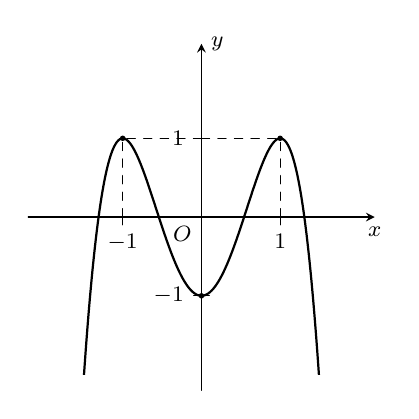
\begin{tikzpicture}[scale=1, font=\footnotesize, line join=round, line cap=round, >=stealth]
			\def\xmin{-2}\def\xmax{2}\def\ymin{-2}\def\ymax{2}
			\draw[->] (\xmin-0.2,0)--(\xmax+0.2,0) node[below] {\footnotesize $x$};
			\draw[->] (0,\ymin-0.2)--(0,\ymax+0.2) node[right] {\footnotesize $y$};
			\draw (0,0) node [below left] {\footnotesize $O$};
			\foreach \x in {-1,1}\draw (\x,0.1)--(\x,-0.1) node [below] {\footnotesize $\x$};
			\foreach \y in {-1,1}\draw (0.1,\y)--(-0.1,\y) node [left] {\footnotesize $\y$};
			\clip (\xmin,\ymin) rectangle (\xmax,\ymax);
			\draw[thick,smooth,samples=200,domain=\xmin:\xmax] plot (\x,{-2*((\x)^4)+4*((\x)^2)+-1});
			\draw[dashed] (0,0)--(0,-1)--(0,-1);\fill (0,-1) circle (1pt);
			\draw[dashed] (1,0)--(1,1)--(0,1);\fill (1,1) circle (1pt);
			\draw[dashed] (-1,0)--(-1,1)--(0,1);\fill (-1,1) circle (1pt);		
		\end{tikzpicture}		
	\end{center}
	\choice
	{$12  $}
	{\True $ 10 $}
	{$ 8 $}
	{$ 4 $}
	\loigiai{ 
		Nhìn vào đồ thị ta thấy $f(x)=0$ có 4 nghiệm phân biệt theo thứ tự $a, b, c, d$.\\		
		Ta có: $f(f(x))=0 \Leftrightarrow\left[\begin{array}{l}f(x)=a, a \in(-\infty ;-1) \\ f(x)=b, b \in(-1 ; 0) \\ f(x)=c, c \in(0 ; 1) \\ f(x)=d, d \in(1 ;+\infty)\end{array}\right.$.
		\definecolor{uuuuuu}{rgb}{0.27,0.27,0.27}
		\begin{center}
			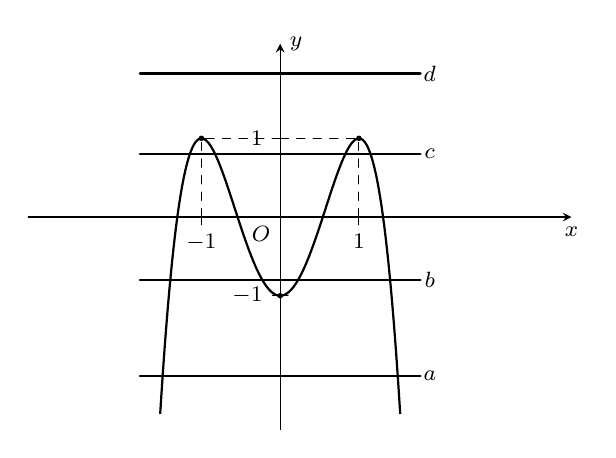
\begin{tikzpicture}[scale=1, font=\footnotesize, line join=round, line cap=round, >=stealth]
				\def\xmin{-3}\def\xmax{3.5}\def\ymin{-2.5}\def\ymax{2}
				\draw[->] (\xmin-0.2,0)--(\xmax+0.2,0) node[below] {\footnotesize $x$};
				\draw[->] (0,\ymin-0.2)--(0,\ymax+0.2) node[right] {\footnotesize $y$};
				\draw (0,0) node [below left] {\footnotesize $O$};
				\foreach \x in {-1,1}\draw (\x,0.1)--(\x,-0.1) node [below] {\footnotesize $\x$};
				\foreach \y in {-1,1}\draw (0.1,\y)--(-0.1,\y) node [left] {\footnotesize $\y$};
				\clip (\xmin,\ymin) rectangle (\xmax,\ymax);
				\draw[thick,smooth,samples=200,domain=\xmin:\xmax] plot (\x,{-2*((\x)^4)+4*((\x)^2)+-1});
				\draw[dashed] (0,0)--(0,-1)--(0,-1);\fill (0,-1) circle (1pt);
				\draw[dashed] (1,0)--(1,1)--(0,1);\fill (1,1) circle (1pt);
				\draw[dashed] (-1,0)--(-1,1)--(0,1);\fill (-1,1) circle (1pt);
				\draw [line width=1.pt] (-1.78,1.82)-- (1.78,1.82);
				\draw [line width=1.pt] (-1.78,0.8)-- (1.78,0.8);
				\draw [line width=1.pt] (-1.78,-0.8)-- (1.78,-0.8);
				\draw [line width=1.pt] (-1.78,-2.02)--(1.78,-2.02);
				\draw[color=black] (1.9,1.82) node {$d$};
				\draw[color=black] (1.9,0.8) node {$c$};
				\draw[color=black] (1.9,-0.8) node {$b$};
				\draw[color=black] (1.9,-2.02) node {$a$};
			\end{tikzpicture}
		\end{center}
		
		Dựa vào đồ thị ta thấy:
		
		Phương trình $f(x)=a$ có 2 nghiệm thực phân biệt.
		
		Phương trình $f(x)=b$ có 4 nghiệm thực phân biệt.
		
		Phương trình $f(x)=c$ có 4 nghiệm thực phân biệt.
		
		Phương trình $f(x)=d$ vô nghiệm trên $\mathbb{R}$.
		
		Vậy phương trình $f(f(x))=0$ có 10 nghiệm thực phân biệt.
	}
\end{ex}

\begin{ex}%[]%[2D1K5-3]
	[Mã 102 - 2021 Lần 1]
	Cho hàm số bậc ba $y=f(x)$ có đồ thị là đường cong trong hình bên. Số nghiệm thực phân biệt của phương trình $f(f(x))=1$ là
	\begin{center}
		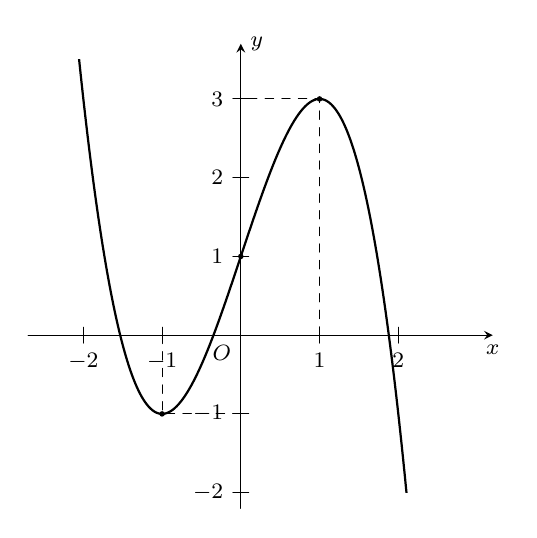
\begin{tikzpicture}[scale=1, font=\footnotesize, line join=round, line cap=round, >=stealth]
			\def\xmin{-2.5}\def\xmax{3}\def\ymin{-2}\def\ymax{3.5}
			\draw[->] (\xmin-0.2,0)--(\xmax+0.2,0) node[below] {\footnotesize $x$};
			\draw[->] (0,\ymin-0.2)--(0,\ymax+0.2) node[right] {\footnotesize $y$};
			\draw (0,0) node [below left] {\footnotesize $O$};
			\foreach \x in {-2,-1,1,2}\draw (\x,0.1)--(\x,-0.1) node [below] {\footnotesize $\x$};
			\foreach \y in {-2,-1,1,2,3}\draw (0.1,\y)--(-0.1,\y) node [left] {\footnotesize $\y$};
			\clip (\xmin,\ymin) rectangle (\xmax,\ymax);
			\draw[thick,smooth,samples=200,domain=\xmin:\xmax] plot (\x,{-1*((\x)^3)+0*((\x)^2)+3*(\x)+1});
			\draw[dashed] (0,0)--(0,1)--(0,1);\fill (0,1) circle (1pt);
			\draw[dashed] (-1,0)--(-1,-1)--(0,-1);\fill (-1,-1) circle (1pt);
			\draw[dashed] (1,0)--(1,3)--(0,3);\fill (1,3) circle (1pt);
		\end{tikzpicture}
	\end{center}
	\choice
	{$9 $}
	{\True $ 7 $}
	{$ 3 $}
	{$ 6 $}
	\loigiai{ 
		Dựa vào đồ thị hàm số $y=f(x)$ suy ra $f(f(x))=1 \Leftrightarrow\left[\begin{array}{l}f(x)=a(a<-1) \\ f(x)=0 \\ f(x)=b(1<b<2)\end{array}\right.$
		\immini{\textbf{	TH1}\\	$f(x)=a \quad(a<-1) \Rightarrow$ phương trình có một nghiệm.}
		{	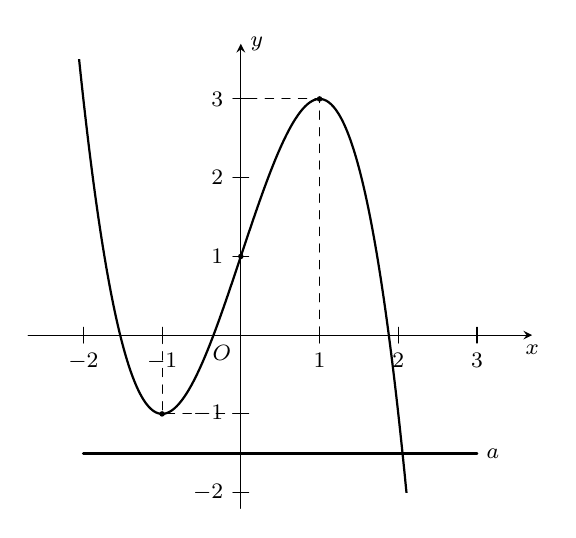
\begin{tikzpicture}[scale=1, font=\footnotesize, line join=round, line cap=round, >=stealth]
				\def\xmin{-2.5}\def\xmax{3.5}\def\ymin{-2}\def\ymax{3.5}
				\draw[->] (\xmin-0.2,0)--(\xmax+0.2,0) node[below] {\footnotesize $x$};
				\draw[->] (0,\ymin-0.2)--(0,\ymax+0.2) node[right] {\footnotesize $y$};
				\draw (0,0) node [below left] {\footnotesize $O$};
				\foreach \x in {-2,-1,1,2,3}\draw (\x,0.1)--(\x,-0.1) node [below] {\footnotesize $\x$};
				\foreach \y in {-2,-1,1,2,3}\draw (0.1,\y)--(-0.1,\y) node [left] {\footnotesize $\y$};
				\clip (\xmin,\ymin) rectangle (\xmax,\ymax);
				\draw[thick,smooth,samples=200,domain=\xmin:\xmax] plot (\x,{-1*((\x)^3)+0*((\x)^2)+3*(\x)+1});
				\draw[dashed] (0,0)--(0,1)--(0,1);\fill (0,1) circle (1pt);
				\draw[dashed] (-1,0)--(-1,-1)--(0,-1);\fill (-1,-1) circle (1pt);
				\draw[dashed] (1,0)--(1,3)--(0,3);\fill (1,3) circle (1pt);
				\draw [line width=1.pt] (-2,-1.5)--(3,-1.5);
				\draw [color=black] (3.2,-1.5) node {$a$} ;
		\end{tikzpicture}}				
		\immini{\textbf{TH2}\\	$f(x)=0 \Rightarrow$ phương trình có ba nghiệm phân biệt.}
		{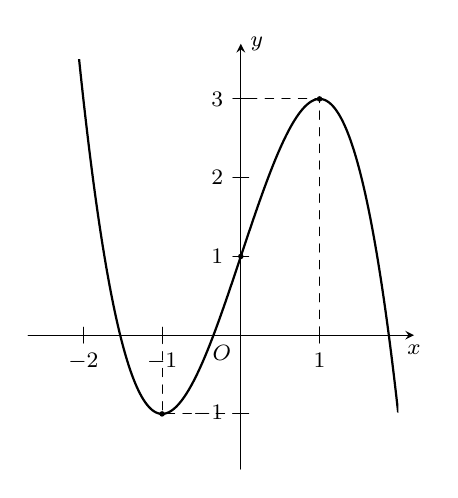
\begin{tikzpicture}[scale=1, font=\footnotesize, line join=round, line cap=round, >=stealth]
				\def\xmin{-2.5}\def\xmax{2}\def\ymin{-1.5}\def\ymax{3.5}
				\draw[->] (\xmin-0.2,0)--(\xmax+0.2,0) node[below] {\footnotesize $x$};
				\draw[->] (0,\ymin-0.2)--(0,\ymax+0.2) node[right] {\footnotesize $y$};
				\draw (0,0) node [below left] {\footnotesize $O$};
				\foreach \x in {-2,-1,1}\draw (\x,0.1)--(\x,-0.1) node [below] {\footnotesize $\x$};
				\foreach \y in {-1,1,2,3}\draw (0.1,\y)--(-0.1,\y) node [left] {\footnotesize $\y$};
				\clip (\xmin,\ymin) rectangle (\xmax,\ymax);
				\draw[thick,smooth,samples=200,domain=\xmin:\xmax] plot (\x,{-1*((\x)^3)+0*((\x)^2)+3*(\x)+1});
				\draw[dashed] (0,0)--(0,1)--(0,1);\fill (0,1) circle (1pt);
				\draw[dashed] (-1,0)--(-1,-1)--(0,-1);\fill (-1,-1) circle (1pt);
				\draw[dashed] (1,0)--(1,3)--(0,3);\fill (1,3) circle (1pt);
		\end{tikzpicture}}		
		\immini{\textbf{TH3:}\\	$f(x)=b(1<b<2) \Rightarrow$ phương trình có ba nghiệm phân biệt.
			
			Các nghiệm của (1); (2); (3) là đôi một khác nhau.
			
			Vậy $f(f(x))=1$ có 7 nghiệm nghiệm phân biệt.}	
		{	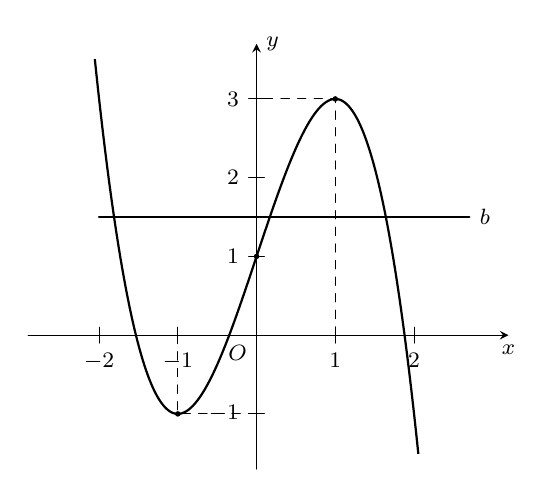
\begin{tikzpicture}[scale=1, font=\footnotesize, line join=round, line cap=round, >=stealth]
				\def\xmin{-2.7}\def\xmax{3}\def\ymin{-1.5}\def\ymax{3.5}
				\draw[->] (\xmin-0.2,0)--(\xmax+0.2,0) node[below] {\footnotesize $x$};
				\draw[->] (0,\ymin-0.2)--(0,\ymax+0.2) node[right] {\footnotesize $y$};
				\draw (0,0) node [below left] {\footnotesize $O$};
				\foreach \x in {-2,-1,1,2}\draw (\x,0.1)--(\x,-0.1) node [below] {\footnotesize $\x$};
				\foreach \y in {-1,1,2,3}\draw (0.1,\y)--(-0.1,\y) node [left] {\footnotesize $\y$};
				\clip (\xmin,\ymin) rectangle (\xmax,\ymax);
				\draw[thick,smooth,samples=200,domain=\xmin:\xmax] plot (\x,{-1*((\x)^3)+0*((\x)^2)+3*(\x)+1});
				\draw[dashed] (0,0)--(0,1)--(0,1);\fill (0,1) circle (1pt);
				\draw[dashed] (-1,0)--(-1,-1)--(0,-1);\fill (-1,-1) circle (1pt);
				\draw[dashed] (1,0)--(1,3)--(0,3);\fill (1,3) circle (1pt);
				\draw [line width=1.pt] (-2,1.5)--(2.7,1.5);
				\draw [color=black] (2.9,1.5) node {$b$} ;
	\end{tikzpicture}}	}
\end{ex}
\begin{ex}%[]%[2D1K5-3]
	[Mã 103 - 2021 - Lần 1] Cho hàm số bậc bốn $y=f(x)$ có đồ thị là đường cong trong hình bên dưới:
	\begin{center}
		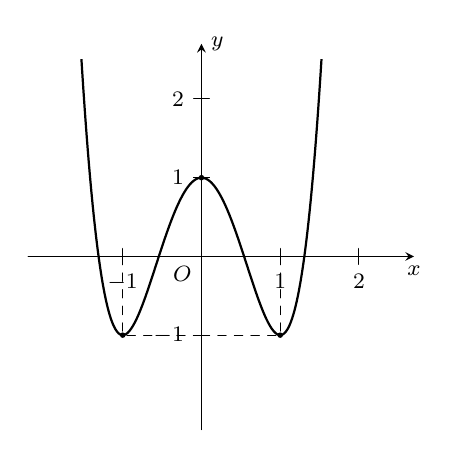
\begin{tikzpicture}[scale=1, font=\footnotesize, line join=round, line cap=round, >=stealth]
			\def\xmin{-2}\def\xmax{2.5}\def\ymin{-2}\def\ymax{2.5}
			\draw[->] (\xmin-0.2,0)--(\xmax+0.2,0) node[below] {\footnotesize $x$};
			\draw[->] (0,\ymin-0.2)--(0,\ymax+0.2) node[right] {\footnotesize $y$};
			\draw (0,0) node [below left] {\footnotesize $O$};
			\foreach \x in {-1,1,2}\draw (\x,0.1)--(\x,-0.1) node [below] {\footnotesize $\x$};
			\foreach \y in {-1,1,2,}\draw (0.1,\y)--(-0.1,\y) node [left] {\footnotesize $\y$};
			\clip (\xmin,\ymin) rectangle (\xmax,\ymax);
			\draw[thick,smooth,samples=200,domain=\xmin:\xmax] plot (\x,{2*((\x)^4)+-4*((\x)^2)+1});
			\draw[dashed] (0,0)--(0,1)--(0,1);\fill (0,1) circle (1pt);
			\draw[dashed] (1,0)--(1,-1)--(0,-1);\fill (1,-1) circle (1pt);
			\draw[dashed] (-1,0)--(-1,-1)--(0,-1);\fill (-1,-1) circle (1pt);
		\end{tikzpicture}		
	\end{center}
	Số nghiệm thực phân biệt của phương trình $f(f(x))=0$ là
	\choice
	{$4  $}
	{\True $10  $}
	{$ 12 $}
	{$ 8 $}
	\loigiai{ 			
		\immini{		Ta có: $f(f(x))=0 \Leftrightarrow\left[\begin{array}{ll}f(x)=a & (a<-1) \\ f(x)=b & (-1<b<0) \\ f(x)=c & (0<c<1) \\ f(x)=d & (d>1)\end{array}\right.$.
			
			Phương trình $f(x)=a$ với $a<-1$ vô nghiệm.
			
			Phương trình $f(x)=b$ với $-1<b<0$ có 4 nghiệm phân biệt.
			
			Phương trình $f(x)=c$ với $0<c<1$ có 4 nghiệm phân biệt.
			
			Phương trình $f(x)=d$ với $d>1$ có 2 nghiệm phân biệt.}
		{	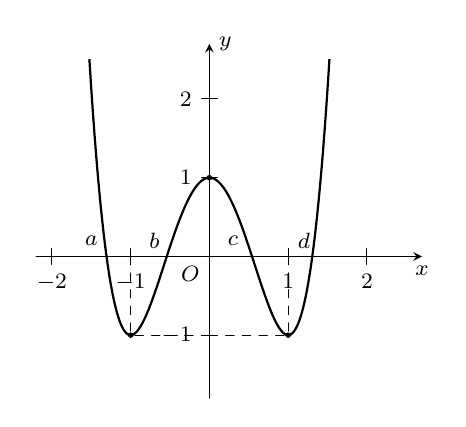
\begin{tikzpicture}[scale=1, font=\footnotesize, line join=round, line cap=round, >=stealth]
				\def\xmin{-2}\def\xmax{2.5}\def\ymin{-1.6}\def\ymax{2.5}
				\draw[->] (\xmin-0.2,0)--(\xmax+0.2,0) node[below] {\footnotesize $x$};
				\draw[->] (0,\ymin-0.2)--(0,\ymax+0.2) node[right] {\footnotesize $y$};
				\draw (0,0) node [below left] {\footnotesize $O$};
				\foreach \x in {-2,-1,1,2,}\draw (\x,0.1)--(\x,-0.1) node [below] {\footnotesize $\x$};
				\foreach \y in {-1,1,2}\draw (0.1,\y)--(-0.1,\y) node [left] {\footnotesize $\y$};
				\clip (\xmin,\ymin) rectangle (\xmax,\ymax);
				\draw[thick,smooth,samples=200,domain=\xmin:\xmax] plot (\x,{2*((\x)^4)+-4*((\x)^2)+1});
				\draw[dashed] (0,0)--(0,1)--(0,1);\fill (0,1) circle (1pt);
				\draw[dashed] (1,0)--(1,-1)--(0,-1);\fill (1,-1) circle (1pt);
				\draw[dashed] (-1,0)--(-1,-1)--(0,-1);\fill (-1,-1) circle (1pt);
				\draw [color=black] (-1.5,0.2) node {$a$};
				\draw [color=black] (-0.7,0.2) node {$b$};
				\draw [color=black] (0.3,0.2) node {$c$};
				\draw [color=black] (1.2,0.2) node {$d$};
	\end{tikzpicture}}	}
\end{ex}
\begin{ex}%[]%[2D1K5-3]
	[Mã 101 - 2021 Lần 1] Cho hàm số bậc ba $y=f(x)$ có đồ thị là đường cong trong hình bên.
	\begin{center}
		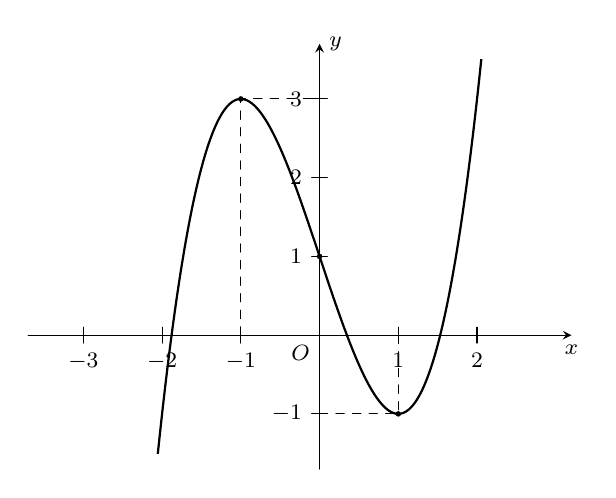
\begin{tikzpicture}[scale=1, font=\footnotesize, line join=round, line cap=round, >=stealth]
			\def\xmin{-3.5}\def\xmax{3}\def\ymin{-1.5}\def\ymax{3.5}
			\draw[->] (\xmin-0.2,0)--(\xmax+0.2,0) node[below] {\footnotesize $x$};
			\draw[->] (0,\ymin-0.2)--(0,\ymax+0.2) node[right] {\footnotesize $y$};
			\draw (0,0) node [below left] {\footnotesize $O$};
			\foreach \x in {-3,-2,-1,1,2}\draw (\x,0.1)--(\x,-0.1) node [below] {\footnotesize $\x$};
			\foreach \y in {-1,1,2,3}\draw (0.1,\y)--(-0.1,\y) node [left] {\footnotesize $\y$};
			\clip (\xmin,\ymin) rectangle (\xmax,\ymax);
			\draw[thick,smooth,samples=200,domain=\xmin:\xmax] plot (\x,{1*((\x)^3)+0*((\x)^2)+-3*(\x)+1});
			\draw[dashed] (0,0)--(0,1)--(0,1);\fill (0,1) circle (1pt);
			\draw[dashed] (-1,0)--(-1,3)--(0,3);\fill (-1,3) circle (1pt);
			\draw[dashed] (1,0)--(1,-1)--(0,-1);\fill (1,-1) circle (1pt);
		\end{tikzpicture}
	\end{center}
	
	Số nghiệm thực phân biệt của phương trình $f(f(x))=1$ là:
	\choice
	{$9  $}
	{$ 3 $}
	{$  6$}
	{\True $ 7 $}
	\loigiai{ 
		Ta có: $f(f(x))=1 \Leftrightarrow\left[\begin{array}{ll}f(x)=0 & \\ f(x)=a & (a<-1) \\ f(x)=b & (1<b<2).\end{array}\right.$\\	
		Ta dựa vào đồ thị:\\		
		Phương trình $f(x)=0$ có 3 nghiệm.\\		
		Phương trình $f(x)=a$ có 1 nghiệm.\\		
		Phương trình $f(x)=b$ có 3 nghiệm.\\
		Vậy phương trình $f(f(x))=1$ có 7 nghiệm phân biệt.
	}
\end{ex}
\begin{ex}%[]%[2D1K5-3]
	[Đề Minh Họa 2020 Lần 1] Cho hàm số $f(x)$ có bảng biến thiên như sau:
	\begin{center}
		
\begin{tikzpicture}
			\tkzTabInit[nocadre=true,lgt=1.2,espcl=2.5,deltacl=0.6]
			{$x$ /0.6,$y’$ /0.6,$y$ /2}
			{$-\infty$,$-1$,$0$,$1$,$+\infty$}
			\tkzTabLine{,-,0,+,0,-,0,+,}
			\tkzTabVar{+/$-\infty$,-/$-2$,+/$-1$,-/$-2$,+/$+\infty$}
		\end{tikzpicture}
	\end{center}
	Số nghiệm thuộc đoạn $[-\pi ; 2 \pi]$ của phương trình $2 f(\sin x)+3=0$ là
	\choice
	{$ 4 $}
	{\True $ 6 $}
	{$ 3 $}
	{$ 8 $}
	\loigiai{		
		Đặt $t=\sin x$. Do $x \in[-\pi ; 2 \pi]$ nên $t \in[-1 ; 1]$.\\	
		Khi đó ta có phương trình $2 f(t)+3=0 \Leftrightarrow f(t)=-\dfrac{3}{2}$.\\	
		Dựa vào bảng biến thiên ta thấy phương trình $f(t)=-\dfrac{3}{2}$ có $2$ nghiệm $t=a \in(-1 ; 0)$ và $t=b \in(0 ; 1)$.\\
		Trường hợp 1: $t=a \in(-1 ; 0)$.\\
		Ứng với mỗi giá trị $t \in(-1 ; 0)$ thì phương trình có $4$ nghiệm $-\pi<x_{1}<x_{2}<0<\pi<x_{3}<x_{4}<2 \pi$.\\
		Trường hợp 2: $t=b \in(0 ; 1)$.\\
		Ứng với mỗi giá trị $t \in(0 ; 1)$ thì phương trình có $4$ nghiệm $0<x_{5}<x_{6}<\pi$.\\
		Hiển nhiên cả $6$ nghiệm trong $2$ trường hợp trên đều khác nhau.\\
		Vậy phương trình đã cho có $6$ nghiệm thuộc đoạn $[-\pi ; 2 \pi]$.		
	}
\end{ex}
\begin{ex}%[]%[2D1K5-3]
	[Đề Tham Khảo 2020 Lần 2] Cho hàm số $f(x)$ có bảng biến thiên như sau
	\begin{center}
		
\begin{tikzpicture}
			\tkzTabInit[nocadre=true,lgt=1.2,espcl=2.5,deltacl=0.6]
			{$x$ /0.6,$y’$ /0.6,$y$ /2}
			{$-\infty$,$-1$,$0$,$1$,$+\infty$}
			\tkzTabLine{,+,0,-,0,+,0,-,}
			\tkzTabVar{-/$-\infty$,+/$2$,-/$0$,+/$2$,-/$-\infty$}
		\end{tikzpicture}
	\end{center}
	\choice
	{$ 7 $}
	{$ 4 $}
	{\True $ 5 $}
	{$ 6 $}
	\loigiai{ 
		Đặt $t=\sin x, x \in\left[0 ; \dfrac{5 \pi}{2}\right] \Rightarrow t \in[-1 ; 1]$.\\
		Khi đó phương trình $f(\sin x)=1$ trở thành $f(t)=1, \forall t \in[-1 ; 1]$.
		\\		Đây là phương trình hoành độ giao điểm của hàm số $y=f(t)$ và đường thẳng $y=1$.\\
		Dựa vào bảng biến thiên, ta có $f(t)=1 \Rightarrow\left[\begin{array}{l}t=a \in(-1 ; 0) \\ t=b \in(0 ; 1).\end{array}\right.$\\
		Trường hợp 1: $t=a \in(-1 ; 0)$.\\
		Ứng với mỗi giá trị $t \in(-1 ; 0)$ thì phương trình $\sin x=t$ có 2 nghiệm $x_{1}, x_{2}$ thỏa mãn $\pi<x_{1}<x_{2}<2 \pi$.\\	
		Trường hợp 2: $t=b \in(0 ; 1)$.\\
		Ứng với mỗi giá trị $t \in(0 ; 1)$ thì phương trình có 3 nghiệm $x_{1}, x_{2}, x_{3}$ thỏa mãn $0<x_{3}<x_{4}<\pi ; 2 \pi<x_{5}<\dfrac{5 \pi}{2}$.\\
		Hiển nhiên cả 5 nghiệm trong 2 trường hợp trên đều khác nhau.\\		
		Vậy phương trình đã cho có 5 nghiệm thuộc đoạn $\left[0 ; \dfrac{5 \pi}{2}\right]$.	}
\end{ex}
\begin{ex}%[]%[2D1K5-3]
	[Mã 101 - 2020 Lần 1] Cho hàm số bậc ba $y=f(x)$ có đồ thị là đường cong trong hình bên. Số nghiệm thực phân biệt của phương trình $f\left(x^3 f(x)\right)+1=0$ là
	\begin{center}
		\definecolor{wwwwww}{rgb}{0.4,0.4,0.4}
		\begin{tikzpicture}[line cap=round,line join=round,>=triangle 45,x=0.8554881008068222cm,y=1.0cm]
			\def\xmin{-2}\def\xmax{4}\def\ymin{-4}\def\ymax{2}
			\draw[->] (\xmin-0.2,0)--(\xmax+2,0) node[below] {\footnotesize $x$};
			\draw[->] (0,\ymin-0.2)--(0,\ymax+0.2) node[right] {\footnotesize $y$};
			\draw (0,0) node [below left] {\footnotesize $O$};
			\clip(-1.1521915641592793,-3.9028423621090513) rectangle (5.767653829770809,1.6406104260940695);
			\draw[line width=2.pt,color=wwwwww] (-0.9248954025048582,-3.3851124077784323) -- (-0.9248954025048582,-3.3851124077784323);
			\draw[line width=2.pt,color=wwwwww] (-0.9248954025048582,-3.3851124077784323) -- (-0.9104849051096838,-3.3536868956202825);
			\draw[line width=2.pt,color=wwwwww] (-0.9104849051096838,-3.3536868956202825) -- (-0.8960744077145094,-3.322257133310096);
			\draw[line width=2.pt,color=wwwwww] (-0.8960744077145094,-3.322257133310096) -- (-0.881663910319335,-3.290827732824434);
			\draw[line width=2.pt,color=wwwwww] (-0.881663910319335,-3.290827732824434) -- (-0.8672534129241606,-3.2594032680505185);
			\draw[line width=2.pt,color=wwwwww] (-0.8672534129241606,-3.2594032680505185) -- (-0.8528429155289862,-3.22798827478623);
			\draw[line width=2.pt,color=wwwwww] (-0.8528429155289862,-3.22798827478623) -- (-0.8384324181338118,-3.1965872507401105);
			\draw[line width=2.pt,color=wwwwww] (-0.8384324181338118,-3.1965872507401105) -- (-0.8240219207386373,-3.1652046555313613);
			\draw[line width=2.pt,color=wwwwww] (-0.8240219207386373,-3.1652046555313613) -- (-0.8096114233434629,-3.133844910689843);
			\draw[line width=2.pt,color=wwwwww] (-0.8096114233434629,-3.133844910689843) -- (-0.7952009259482885,-3.102512399656076);
			\draw[line width=2.pt,color=wwwwww] (-0.7952009259482885,-3.102512399656076) -- (-0.7807904285531141,-3.071211467781242);
			\draw[line width=2.pt,color=wwwwww] (-0.7807904285531141,-3.071211467781242) -- (-0.7663799311579397,-3.0399464223271817);
			\draw[line width=2.pt,color=wwwwww] (-0.7663799311579397,-3.0399464223271817) -- (-0.7519694337627653,-3.008721532466396);
			\draw[line width=2.pt,color=wwwwww] (-0.7519694337627653,-3.008721532466396) -- (-0.7375589363675908,-2.977541029282045);
			\draw[line width=2.pt,color=wwwwww] (-0.7375589363675908,-2.977541029282045) -- (-0.7231484389724164,-2.946409105767949);
			\draw[line width=2.pt,color=wwwwww] (-0.7231484389724164,-2.946409105767949) -- (-0.708737941577242,-2.915329916828589);
			\draw[line width=2.pt,color=wwwwww] (-0.708737941577242,-2.915329916828589) -- (-0.6943274441820676,-2.8843075792791053);
			\draw[line width=2.pt,color=wwwwww] (-0.6943274441820676,-2.8843075792791053) -- (-0.6799169467868932,-2.8533461718452973);
			\draw[line width=2.pt,color=wwwwww] (-0.6799169467868932,-2.8533461718452973) -- (-0.6655064493917188,-2.822449735163626);
			\draw[line width=2.pt,color=wwwwww] (-0.6655064493917188,-2.822449735163626) -- (-0.6510959519965444,-2.7916222717812116);
			\draw[line width=2.pt,color=wwwwww] (-0.6510959519965444,-2.7916222717812116) -- (-0.6366854546013699,-2.7608677461558333);
			\draw[line width=2.pt,color=wwwwww] (-0.6366854546013699,-2.7608677461558333) -- (-0.6222749572061955,-2.7301900846559315);
			\draw[line width=2.pt,color=wwwwww] (-0.6222749572061955,-2.7301900846559315) -- (-0.6078644598110211,-2.6995931755606053);
			\draw[line width=2.pt,color=wwwwww] (-0.6078644598110211,-2.6995931755606053) -- (-0.5934539624158467,-2.6690808690596155);
			\draw[line width=2.pt,color=wwwwww] (-0.5934539624158467,-2.6690808690596155) -- (-0.5790434650206723,-2.6386569772533806);
			\draw[line width=2.pt,color=wwwwww] (-0.5790434650206723,-2.6386569772533806) -- (-0.5646329676254979,-2.608325274152981);
			\draw[line width=2.pt,color=wwwwww] (-0.5646329676254979,-2.608325274152981) -- (-0.5502224702303234,-2.578089495680155);
			\draw[line width=2.pt,color=wwwwww] (-0.5502224702303234,-2.578089495680155) -- (-0.535811972835149,-2.547953339667303);
			\draw[line width=2.pt,color=wwwwww] (-0.535811972835149,-2.547953339667303) -- (-0.5214014754399746,-2.5179204658574834);
			\draw[line width=2.pt,color=wwwwww] (-0.5214014754399746,-2.5179204658574834) -- (-0.5069909780448002,-2.487994495904416);
			\draw[line width=2.pt,color=wwwwww] (-0.5069909780448002,-2.487994495904416) -- (-0.4925804806496258,-2.4581790133724795);
			\draw[line width=2.pt,color=wwwwww] (-0.4925804806496258,-2.4581790133724795) -- (-0.47816998325445137,-2.4284775637367124);
			\draw[line width=2.pt,color=wwwwww] (-0.47816998325445137,-2.4284775637367124) -- (-0.46375948585927695,-2.3988936543828143);
			\draw[line width=2.pt,color=wwwwww] (-0.46375948585927695,-2.3988936543828143) -- (-0.44934898846410254,-2.3694307546071434);
			\draw[line width=2.pt,color=wwwwww] (-0.44934898846410254,-2.3694307546071434) -- (-0.4349384910689281,-2.340092295616719);
			\draw[line width=2.pt,color=wwwwww] (-0.4349384910689281,-2.340092295616719) -- (-0.4205279936737537,-2.310881670529219);
			\draw[line width=2.pt,color=wwwwww] (-0.4205279936737537,-2.310881670529219) -- (-0.4061174962785793,-2.2818022343729822);
			\draw[line width=2.pt,color=wwwwww] (-0.4061174962785793,-2.2818022343729822) -- (-0.3917069988834049,-2.252857304087007);
			\draw[line width=2.pt,color=wwwwww] (-0.3917069988834049,-2.252857304087007) -- (-0.37729650148823046,-2.224050158520951);
			\draw[line width=2.pt,color=wwwwww] (-0.37729650148823046,-2.224050158520951) -- (-0.36288600409305605,-2.195384038435134);
			\draw[line width=2.pt,color=wwwwww] (-0.36288600409305605,-2.195384038435134) -- (-0.34847550669788163,-2.166862146500532);
			\draw[line width=2.pt,color=wwwwww] (-0.34847550669788163,-2.166862146500532) -- (-0.3340650093027072,-2.138487647298785);
			\draw[line width=2.pt,color=wwwwww] (-0.3340650093027072,-2.138487647298785) -- (-0.3196545119075328,-2.1102636673221897);
			\draw[line width=2.pt,color=wwwwww] (-0.3196545119075328,-2.1102636673221897) -- (-0.3052440145123584,-2.0821932949737043);
			\draw[line width=2.pt,color=wwwwww] (-0.3052440145123584,-2.0821932949737043) -- (-0.29083351711718397,-2.0542795805669467);
			\draw[line width=2.pt,color=wwwwww] (-0.29083351711718397,-2.0542795805669467) -- (-0.27642301972200956,-2.0265255363261945);
			\draw[line width=2.pt,color=wwwwww] (-0.27642301972200956,-2.0265255363261945) -- (-0.26201252232683514,-1.9989341363863848);
			\draw[line width=2.pt,color=wwwwww] (-0.26201252232683514,-1.9989341363863848) -- (-0.24760202493166072,-1.9715083167931156);
			\draw[line width=2.pt,color=wwwwww] (-0.24760202493166072,-1.9715083167931156) -- (-0.2331915275364863,-1.9442509755026438);
			\draw[line width=2.pt,color=wwwwww] (-0.2331915275364863,-1.9442509755026438) -- (-0.2187810301413119,-1.9171649723818873);
			\draw[line width=2.pt,color=wwwwww] (-0.2187810301413119,-1.9171649723818873) -- (-0.20437053274613748,-1.8902531292084228);
			\draw[line width=2.pt,color=wwwwww] (-0.20437053274613748,-1.8902531292084228) -- (-0.18996003535096306,-1.8635182296704875);
			\draw[line width=2.pt,color=wwwwww] (-0.18996003535096306,-1.8635182296704875) -- (-0.17554953795578865,-1.8369630193669784);
			\draw[line width=2.pt,color=wwwwww] (-0.17554953795578865,-1.8369630193669784) -- (-0.16113904056061423,-1.8105902058074523);
			\draw[line width=2.pt,color=wwwwww] (-0.16113904056061423,-1.8105902058074523) -- (-0.14672854316543982,-1.7844024584121263);
			\draw[line width=2.pt,color=wwwwww] (-0.14672854316543982,-1.7844024584121263) -- (-0.1323180457702654,-1.758402408511877);
			\draw[line width=2.pt,color=wwwwww] (-0.1323180457702654,-1.758402408511877) -- (-0.11790754837509099,-1.732592649348241);
			\draw[line width=2.pt,color=wwwwww] (-0.11790754837509099,-1.732592649348241) -- (-0.10349705097991657,-1.706975736073415);
			\draw[line width=2.pt,color=wwwwww] (-0.10349705097991657,-1.706975736073415) -- (-0.08908655358474216,-1.681554185750255);
			\draw[line width=2.pt,color=wwwwww] (-0.08908655358474216,-1.681554185750255) -- (-0.07467605618956774,-1.6563304773522778);
			\draw[line width=2.pt,color=wwwwww] (-0.07467605618956774,-1.6563304773522778) -- (-0.06026555879439333,-1.6313070517636596);
			\draw[line width=2.pt,color=wwwwww] (-0.06026555879439333,-1.6313070517636596) -- (-0.045855061399218924,-1.6064863117792365);
			\draw[line width=2.pt,color=wwwwww] (-0.045855061399218924,-1.6064863117792365) -- (-0.031444564004044516,-1.5818706221045045);
			\draw[line width=2.pt,color=wwwwww] (-0.031444564004044516,-1.5818706221045045) -- (-0.017034066608870108,-1.5574623093556197);
			\draw[line width=2.pt,color=wwwwww] (-0.017034066608870108,-1.5574623093556197) -- (-0.0026235692136956975,-1.533263662059398);
			\draw[line width=2.pt,color=wwwwww] (-0.0026235692136956975,-1.533263662059398) -- (0.011786928181478713,-1.5092769306533151);
			\draw[line width=2.pt,color=wwwwww] (0.011786928181478713,-1.5092769306533151) -- (0.026197425576653124,-1.4855043274855069);
			\draw[line width=2.pt,color=wwwwww] (0.026197425576653124,-1.4855043274855069) -- (0.04060792297182753,-1.4619480268147687);
			\draw[line width=2.pt,color=wwwwww] (0.04060792297182753,-1.4619480268147687) -- (0.05501842036700194,-1.4386101648105563);
			\draw[line width=2.pt,color=wwwwww] (0.05501842036700194,-1.4386101648105563) -- (0.06942891776217636,-1.415492839552985);
			\draw[line width=2.pt,color=wwwwww] (0.06942891776217636,-1.415492839552985) -- (0.08383941515735077,-1.3925981110328305);
			\draw[line width=2.pt,color=wwwwww] (0.08383941515735077,-1.3925981110328305) -- (0.09824991255252519,-1.3699280011515274);
			\draw[line width=2.pt,color=wwwwww] (0.09824991255252519,-1.3699280011515274) -- (0.1126604099476996,-1.3474844937211714);
			\draw[line width=2.pt,color=wwwwww] (0.1126604099476996,-1.3474844937211714) -- (0.12707090734287402,-1.3252695344645173);
			\draw[line width=2.pt,color=wwwwww] (0.12707090734287402,-1.3252695344645173) -- (0.14148140473804843,-1.3032850310149802);
			\draw[line width=2.pt,color=wwwwww] (0.14148140473804843,-1.3032850310149802) -- (0.15589190213322285,-1.281532852916635);
			\draw[line width=2.pt,color=wwwwww] (0.15589190213322285,-1.281532852916635) -- (0.17030239952839726,-1.2600148316242163);
			\draw[line width=2.pt,color=wwwwww] (0.17030239952839726,-1.2600148316242163) -- (0.18471289692357168,-1.2387327605031189);
			\draw[line width=2.pt,color=wwwwww] (0.18471289692357168,-1.2387327605031189) -- (0.1991233943187461,-1.2176883948293975);
			\draw[line width=2.pt,color=wwwwww] (0.1991233943187461,-1.2176883948293975) -- (0.2135338917139205,-1.1968834517897666);
			\draw[line width=2.pt,color=wwwwww] (0.2135338917139205,-1.1968834517897666) -- (0.22794438910909492,-1.1763196104816007);
			\draw[line width=2.pt,color=wwwwww] (0.22794438910909492,-1.1763196104816007) -- (0.24235488650426934,-1.1559985119129337);
			\draw[line width=2.pt,color=wwwwww] (0.24235488650426934,-1.1559985119129337) -- (0.25676538389944376,-1.1359217590024602);
			\draw[line width=2.pt,color=wwwwww] (0.25676538389944376,-1.1359217590024602) -- (0.27117588129461817,-1.1160909165795345);
			\draw[line width=2.pt,color=wwwwww] (0.27117588129461817,-1.1160909165795345) -- (0.2855863786897926,-1.0965075113841702);
			\draw[line width=2.pt,color=wwwwww] (0.2855863786897926,-1.0965075113841702) -- (0.299996876084967,-1.0771730320670416);
			\draw[line width=2.pt,color=wwwwww] (0.299996876084967,-1.0771730320670416) -- (0.3144073734801414,-1.0580889291894824);
			\draw[line width=2.pt,color=wwwwww] (0.3144073734801414,-1.0580889291894824) -- (0.32881787087531583,-1.0392566152234866);
			\draw[line width=2.pt,color=wwwwww] (0.32881787087531583,-1.0392566152234866) -- (0.34322836827049025,-1.0206774645517074);
			\draw[line width=2.pt,color=wwwwww] (0.34322836827049025,-1.0206774645517074) -- (0.35763886566566466,-1.002352813467459);
			\draw[line width=2.pt,color=wwwwww] (0.35763886566566466,-1.002352813467459) -- (0.3720493630608391,-0.9842839601747145);
			\draw[line width=2.pt,color=wwwwww] (0.3720493630608391,-0.9842839601747145) -- (0.3864598604560135,-0.9664721647881075);
			\draw[line width=2.pt,color=wwwwww] (0.3864598604560135,-0.9664721647881075) -- (0.4008703578511879,-0.9489186493329311);
			\draw[line width=2.pt,color=wwwwww] (0.4008703578511879,-0.9489186493329311) -- (0.4152808552463623,-0.9316245977451388);
			\draw[line width=2.pt,color=wwwwww] (0.4152808552463623,-0.9316245977451388) -- (0.42969135264153674,-0.9145911558713437);
			\draw[line width=2.pt,color=wwwwww] (0.42969135264153674,-0.9145911558713437) -- (0.44410185003671115,-0.8978194314688186);
			\draw[line width=2.pt,color=wwwwww] (0.44410185003671115,-0.8978194314688186) -- (0.45851234743188557,-0.8813104942054966);
			\draw[line width=2.pt,color=wwwwww] (0.45851234743188557,-0.8813104942054966) -- (0.47292284482706,-0.8650653756599704);
			\draw[line width=2.pt,color=wwwwww] (0.47292284482706,-0.8650653756599704) -- (0.4873333422222344,-0.8490850693214931);
			\draw[line width=2.pt,color=wwwwww] (0.4873333422222344,-0.8490850693214931) -- (0.5017438396174088,-0.833370530589977);
			\draw[line width=2.pt,color=wwwwww] (0.5017438396174088,-0.833370530589977) -- (0.5161543370125832,-0.817922676775995);
			\draw[line width=2.pt,color=wwwwww] (0.5161543370125832,-0.817922676775995) -- (0.5305648344077576,-0.8027423871007793);
			\draw[line width=2.pt,color=wwwwww] (0.5305648344077576,-0.8027423871007793) -- (0.544975331802932,-0.7878305026962225);
			\draw[line width=2.pt,color=wwwwww] (0.544975331802932,-0.7878305026962225) -- (0.5593858291981064,-0.7731878266048767);
			\draw[line width=2.pt,color=wwwwww] (0.5593858291981064,-0.7731878266048767) -- (0.5737963265932808,-0.7588151237799544);
			\draw[line width=2.pt,color=wwwwww] (0.5737963265932808,-0.7588151237799544) -- (0.5882068239884553,-0.7447131210853275);
			\draw[line width=2.pt,color=wwwwww] (0.5882068239884553,-0.7447131210853275) -- (0.6026173213836297,-0.7308825072955282);
			\draw[line width=2.pt,color=wwwwww] (0.6026173213836297,-0.7308825072955282) -- (0.6170278187788041,-0.717323933095748);
			\draw[line width=2.pt,color=wwwwww] (0.6170278187788041,-0.717323933095748) -- (0.6314383161739785,-0.7040380110818394);
			\draw[line width=2.pt,color=wwwwww] (0.6314383161739785,-0.7040380110818394) -- (0.6458488135691529,-0.6910253157603136);
			\draw[line width=2.pt,color=wwwwww] (0.6458488135691529,-0.6910253157603136) -- (0.6602593109643273,-0.6782863835483426);
			\draw[line width=2.pt,color=wwwwww] (0.6602593109643273,-0.6782863835483426) -- (0.6746698083595017,-0.6658217127737577);
			\draw[line width=2.pt,color=wwwwww] (0.6746698083595017,-0.6658217127737577) -- (0.6890803057546762,-0.6536317636750506);
			\draw[line width=2.pt,color=wwwwww] (0.6890803057546762,-0.6536317636750506) -- (0.7034908031498506,-0.6417169584013727);
			\draw[line width=2.pt,color=wwwwww] (0.7034908031498506,-0.6417169584013727) -- (0.717901300545025,-0.6300776810125348);
			\draw[line width=2.pt,color=wwwwww] (0.717901300545025,-0.6300776810125348) -- (0.7323117979401994,-0.6187142774790089);
			\draw[line width=2.pt,color=wwwwww] (0.7323117979401994,-0.6187142774790089) -- (0.7467222953353738,-0.6076270556819252);
			\draw[line width=2.pt,color=wwwwww] (0.7467222953353738,-0.6076270556819252) -- (0.7611327927305482,-0.5968162854130756);
			\draw[line width=2.pt,color=wwwwww] (0.7611327927305482,-0.5968162854130756) -- (0.7755432901257227,-0.5862821983749102);
			\draw[line width=2.pt,color=wwwwww] (0.7755432901257227,-0.5862821983749102) -- (0.7899537875208971,-0.5760249881805406);
			\draw[line width=2.pt,color=wwwwww] (0.7899537875208971,-0.5760249881805406) -- (0.8043642849160715,-0.566044810353737);
			\draw[line width=2.pt,color=wwwwww] (0.8043642849160715,-0.566044810353737) -- (0.8187747823112459,-0.5563417823289303);
			\draw[line width=2.pt,color=wwwwww] (0.8187747823112459,-0.5563417823289303) -- (0.8331852797064203,-0.5469159834512107);
			\draw[line width=2.pt,color=wwwwww] (0.8331852797064203,-0.5469159834512107) -- (0.8475957771015947,-0.5377674549763292);
			\draw[line width=2.pt,color=wwwwww] (0.8475957771015947,-0.5377674549763292) -- (0.8620062744967691,-0.5288962000706959);
			\draw[line width=2.pt,color=wwwwww] (0.8620062744967691,-0.5288962000706959) -- (0.8764167718919436,-0.5203021838113808);
			\draw[line width=2.pt,color=wwwwww] (0.8764167718919436,-0.5203021838113808) -- (0.890827269287118,-0.5119853331861146);
			\draw[line width=2.pt,color=wwwwww] (0.890827269287118,-0.5119853331861146) -- (0.9052377666822924,-0.503945537093287);
			\draw[line width=2.pt,color=wwwwww] (0.9052377666822924,-0.503945537093287) -- (0.9196482640774668,-0.4961826463419481);
			\draw[line width=2.pt,color=wwwwww] (0.9196482640774668,-0.4961826463419481) -- (0.9340587614726412,-0.4886964736518078);
			\draw[line width=2.pt,color=wwwwww] (0.9340587614726412,-0.4886964736518078) -- (0.9484692588678156,-0.4814867936532361);
			\draw[line width=2.pt,color=wwwwww] (0.9484692588678156,-0.4814867936532361) -- (0.96287975626299,-0.47455334288726236);
			\draw[line width=2.pt,color=wwwwww] (0.96287975626299,-0.47455334288726236) -- (0.9772902536581645,-0.4678958198055767);
			\draw[line width=2.pt,color=wwwwww] (0.9772902536581645,-0.4678958198055767) -- (0.9917007510533389,-0.461513884770528);
			\draw[line width=2.pt,color=wwwwww] (0.9917007510533389,-0.461513884770528) -- (1.0061112484485133,-0.4554071600551266);
			\draw[line width=2.pt,color=wwwwww] (1.0061112484485133,-0.4554071600551266) -- (1.0205217458436877,-0.4495752298430409);
			\draw[line width=2.pt,color=wwwwww] (1.0205217458436877,-0.4495752298430409) -- (1.0349322432388621,-0.4440176402286009);
			\draw[line width=2.pt,color=wwwwww] (1.0349322432388621,-0.4440176402286009) -- (1.0493427406340365,-0.4387338992167953);
			\draw[line width=2.pt,color=wwwwww] (1.0493427406340365,-0.4387338992167953) -- (1.063753238029211,-0.43372347672327294);
			\draw[line width=2.pt,color=wwwwww] (1.063753238029211,-0.43372347672327294) -- (1.0781637354243854,-0.428985804574344);
			\draw[line width=2.pt,color=wwwwww] (1.0781637354243854,-0.428985804574344) -- (1.0925742328195598,-0.424520276506976);
			\draw[line width=2.pt,color=wwwwww] (1.0925742328195598,-0.424520276506976) -- (1.1069847302147342,-0.4203262481687986);
			\draw[line width=2.pt,color=wwwwww] (1.1069847302147342,-0.4203262481687986) -- (1.1213952276099086,-0.4164030371181);
			\draw[line width=2.pt,color=wwwwww] (1.1213952276099086,-0.4164030371181) -- (1.135805725005083,-0.41274992282382916);
			\draw[line width=2.pt,color=wwwwww] (1.135805725005083,-0.41274992282382916) -- (1.1502162224002574,-0.40936614666559445);
			\draw[line width=2.pt,color=wwwwww] (1.1502162224002574,-0.40936614666559445) -- (1.1646267197954319,-0.4062509119336646);
			\draw[line width=2.pt,color=wwwwww] (1.1646267197954319,-0.4062509119336646) -- (1.1790372171906063,-0.40340338382896723);
			\draw[line width=2.pt,color=wwwwww] (1.1790372171906063,-0.40340338382896723) -- (1.1934477145857807,-0.4008226894630913);
			\draw[line width=2.pt,color=wwwwww] (1.1934477145857807,-0.4008226894630913) -- (1.207858211980955,-0.39850791785828465);
			\draw[line width=2.pt,color=wwwwww] (1.207858211980955,-0.39850791785828465) -- (1.2222687093761295,-0.3964581199474555);
			\draw[line width=2.pt,color=wwwwww] (1.2222687093761295,-0.3964581199474555) -- (1.236679206771304,-0.39467230857417146);
			\draw[line width=2.pt,color=wwwwww] (1.236679206771304,-0.39467230857417146) -- (1.2510897041664784,-0.3931494584926609);
			\draw[line width=2.pt,color=wwwwww] (1.2510897041664784,-0.3931494584926609) -- (1.2655002015616528,-0.3918885063678115);
			\draw[line width=2.pt,color=wwwwww] (1.2655002015616528,-0.3918885063678115) -- (1.2799106989568272,-0.3908883507751706);
			\draw[line width=2.pt,color=wwwwww] (1.2799106989568272,-0.3908883507751706) -- (1.2943211963520016,-0.3901478522009456);
			\draw[line width=2.pt,color=wwwwww] (1.2943211963520016,-0.3901478522009456) -- (1.308731693747176,-0.3896658330420051);
			\draw[line width=2.pt,color=wwwwww] (1.308731693747176,-0.3896658330420051) -- (1.3231421911423504,-0.38944107760587565);
			\draw[line width=2.pt,color=wwwwww] (1.3231421911423504,-0.38944107760587565) -- (1.3375526885375248,-0.38947233211074517);
			\draw[line width=2.pt,color=wwwwww] (1.3375526885375248,-0.38947233211074517) -- (1.3519631859326993,-0.38975830468546);
			\draw[line width=2.pt,color=wwwwww] (1.3519631859326993,-0.38975830468546) -- (1.3663736833278737,-0.3902976653695276);
			\draw[line width=2.pt,color=wwwwww] (1.3663736833278737,-0.3902976653695276) -- (1.380784180723048,-0.39108904611311557);
			\draw[line width=2.pt,color=wwwwww] (1.380784180723048,-0.39108904611311557) -- (1.3951946781182225,-0.39213104077705063);
			\draw[line width=2.pt,color=wwwwww] (1.3951946781182225,-0.39213104077705063) -- (1.409605175513397,-0.39342220513281934);
			\draw[line width=2.pt,color=wwwwww] (1.409605175513397,-0.39342220513281934) -- (1.4240156729085713,-0.3949610568625683);
			\draw[line width=2.pt,color=wwwwww] (1.4240156729085713,-0.3949610568625683) -- (1.4384261703037458,-0.3967460755591048);
			\draw[line width=2.pt,color=wwwwww] (1.4384261703037458,-0.3967460755591048) -- (1.4528366676989202,-0.3987757027258956);
			\draw[line width=2.pt,color=wwwwww] (1.4528366676989202,-0.3987757027258956) -- (1.4672471650940946,-0.4010483417770665);
			\draw[line width=2.pt,color=wwwwww] (1.4672471650940946,-0.4010483417770665) -- (1.481657662489269,-0.4035623580374037);
			\draw[line width=2.pt,color=wwwwww] (1.481657662489269,-0.4035623580374037) -- (1.4960681598844434,-0.4063160787423543);
			\draw[line width=2.pt,color=wwwwww] (1.4960681598844434,-0.4063160787423543) -- (1.5104786572796178,-0.40930779303802467);
			\draw[line width=2.pt,color=wwwwww] (1.5104786572796178,-0.40930779303802467) -- (1.5248891546747922,-0.41253575198117987);
			\draw[line width=2.pt,color=wwwwww] (1.5248891546747922,-0.41253575198117987) -- (1.5392996520699667,-0.41599816853924687);
			\draw[line width=2.pt,color=wwwwww] (1.5392996520699667,-0.41599816853924687) -- (1.553710149465141,-0.41969321759031075);
			\draw[line width=2.pt,color=wwwwww] (1.553710149465141,-0.41969321759031075) -- (1.5681206468603155,-0.42361903592311867);
			\draw[line width=2.pt,color=wwwwww] (1.5681206468603155,-0.42361903592311867) -- (1.58253114425549,-0.4277737222370752);
			\draw[line width=2.pt,color=wwwwww] (1.58253114425549,-0.4277737222370752) -- (1.5969416416506643,-0.4321553371422464);
			\draw[line width=2.pt,color=wwwwww] (1.5969416416506643,-0.4321553371422464) -- (1.6113521390458387,-0.4367619031593575);
			\draw[line width=2.pt,color=wwwwww] (1.6113521390458387,-0.4367619031593575) -- (1.6257626364410132,-0.44159140471979463);
			\draw[line width=2.pt,color=wwwwww] (1.6257626364410132,-0.44159140471979463) -- (1.6401731338361876,-0.4466417881656033);
			\draw[line width=2.pt,color=wwwwww] (1.6401731338361876,-0.4466417881656033) -- (1.654583631231362,-0.45191096174948786);
			\draw[line width=2.pt,color=wwwwww] (1.654583631231362,-0.45191096174948786) -- (1.6689941286265364,-0.4573967956348144);
			\draw[line width=2.pt,color=wwwwww] (1.6689941286265364,-0.4573967956348144) -- (1.6834046260217108,-0.46309712189560726);
			\draw[line width=2.pt,color=wwwwww] (1.6834046260217108,-0.46309712189560726) -- (1.6978151234168852,-0.46900973451655226);
			\draw[line width=2.pt,color=wwwwww] (1.6978151234168852,-0.46900973451655226) -- (1.7122256208120596,-0.47513238939299374);
			\draw[line width=2.pt,color=wwwwww] (1.7122256208120596,-0.47513238939299374) -- (1.726636118207234,-0.481462804330937);
			\draw[line width=2.pt,color=wwwwww] (1.726636118207234,-0.481462804330937) -- (1.7410466156024085,-0.4879986590470462);
			\draw[line width=2.pt,color=wwwwww] (1.7410466156024085,-0.4879986590470462) -- (1.755457112997583,-0.49473759516864657);
			\draw[line width=2.pt,color=wwwwww] (1.755457112997583,-0.49473759516864657) -- (1.7698676103927573,-0.5016772162337224);
			\draw[line width=2.pt,color=wwwwww] (1.7698676103927573,-0.5016772162337224) -- (1.7842781077879317,-0.5088150876909181);
			\draw[line width=2.pt,color=wwwwww] (1.7842781077879317,-0.5088150876909181) -- (1.7986886051831061,-0.5161487368995381);
			\draw[line width=2.pt,color=wwwwww] (1.7986886051831061,-0.5161487368995381) -- (1.8130991025782806,-0.5236756531295468);
			\draw[line width=2.pt,color=wwwwww] (1.8130991025782806,-0.5236756531295468) -- (1.827509599973455,-0.5313932875615683);
			\draw[line width=2.pt,color=wwwwww] (1.827509599973455,-0.5313932875615683) -- (1.8419200973686294,-0.5392990532868871);
			\draw[line width=2.pt,color=wwwwww] (1.8419200973686294,-0.5392990532868871) -- (1.8563305947638038,-0.5473903253074464);
			\draw[line width=2.pt,color=wwwwww] (1.8563305947638038,-0.5473903253074464) -- (1.8707410921589782,-0.5556644405358502);
			\draw[line width=2.pt,color=wwwwww] (1.8707410921589782,-0.5556644405358502) -- (1.8851515895541526,-0.5641186977953634);
			\draw[line width=2.pt,color=wwwwww] (1.8851515895541526,-0.5641186977953634) -- (1.899562086949327,-0.5727503578199085);
			\draw[line width=2.pt,color=wwwwww] (1.899562086949327,-0.5727503578199085) -- (1.9139725843445015,-0.58155664325407);
			\draw[line width=2.pt,color=wwwwww] (1.9139725843445015,-0.58155664325407) -- (1.9283830817396759,-0.5905347386530901);
			\draw[line width=2.pt,color=wwwwww] (1.9283830817396759,-0.5905347386530901) -- (1.9427935791348503,-0.5996817904828742);
			\draw[line width=2.pt,color=wwwwww] (1.9427935791348503,-0.5996817904828742) -- (1.9572040765300247,-0.6089949071199849);
			\draw[line width=2.pt,color=wwwwww] (1.9572040765300247,-0.6089949071199849) -- (1.9716145739251991,-0.6184711588516447);
			\draw[line width=2.pt,color=wwwwww] (1.9716145739251991,-0.6184711588516447) -- (1.9860250713203735,-0.628107577875737);
			\draw[line width=2.pt,color=wwwwww] (1.9860250713203735,-0.628107577875737) -- (2.000435568715548,-0.6379011583008061);
			\draw[line width=2.pt,color=wwwwww] (2.000435568715548,-0.6379011583008061) -- (2.014846066110722,-0.6478488561460534);
			\draw[line width=2.pt,color=wwwwww] (2.014846066110722,-0.6478488561460534) -- (2.0292565635058963,-0.6579475893413429);
			\draw[line width=2.pt,color=wwwwww] (2.0292565635058963,-0.6579475893413429) -- (2.0436670609010705,-0.6681942377271968);
			\draw[line width=2.pt,color=wwwwww] (2.0436670609010705,-0.6681942377271968) -- (2.0580775582962447,-0.6785856430547978);
			\draw[line width=2.pt,color=wwwwww] (2.0580775582962447,-0.6785856430547978) -- (2.072488055691419,-0.6891186089859893);
			\draw[line width=2.pt,color=wwwwww] (2.072488055691419,-0.6891186089859893) -- (2.086898553086593,-0.6997899010932729);
			\draw[line width=2.pt,color=wwwwww] (2.086898553086593,-0.6997899010932729) -- (2.1013090504817673,-0.7105962468598119);
			\draw[line width=2.pt,color=wwwwww] (2.1013090504817673,-0.7105962468598119) -- (2.1157195478769415,-0.7215343356794275);
			\draw[line width=2.pt,color=wwwwww] (2.1157195478769415,-0.7215343356794275) -- (2.1301300452721157,-0.7326008188566031);
			\draw[line width=2.pt,color=wwwwww] (2.1301300452721157,-0.7326008188566031) -- (2.14454054266729,-0.74379230960648);
			\draw[line width=2.pt,color=wwwwww] (2.14454054266729,-0.74379230960648) -- (2.158951040062464,-0.7551053830548615);
			\draw[line width=2.pt,color=wwwwww] (2.158951040062464,-0.7551053830548615) -- (2.1733615374576383,-0.7665365762382086);
			\draw[line width=2.pt,color=wwwwww] (2.1733615374576383,-0.7665365762382086) -- (2.1877720348528125,-0.7780823881036425);
			\draw[line width=2.pt,color=wwwwww] (2.1877720348528125,-0.7780823881036425) -- (2.2021825322479867,-0.7897392795089466);
			\draw[line width=2.pt,color=wwwwww] (2.2021825322479867,-0.7897392795089466) -- (2.216593029643161,-0.8015036732225611);
			\draw[line width=2.pt,color=wwwwww] (2.216593029643161,-0.8015036732225611) -- (2.231003527038335,-0.8133719539235895);
			\draw[line width=2.pt,color=wwwwww] (2.231003527038335,-0.8133719539235895) -- (2.2454140244335092,-0.8253404682017922);
			\draw[line width=2.pt,color=wwwwww] (2.2454140244335092,-0.8253404682017922) -- (2.2598245218286834,-0.8374055245575898);
			\draw[line width=2.pt,color=wwwwww] (2.2598245218286834,-0.8374055245575898) -- (2.2742350192238576,-0.8495633934020645);
			\draw[line width=2.pt,color=wwwwww] (2.2742350192238576,-0.8495633934020645) -- (2.288645516619032,-0.8618103070569574);
			\draw[line width=2.pt,color=wwwwww] (2.288645516619032,-0.8618103070569574) -- (2.303056014014206,-0.8741424597546703);
			\draw[line width=2.pt,color=wwwwww] (2.303056014014206,-0.8741424597546703) -- (2.31746651140938,-0.8865560076382635);
			\draw[line width=2.pt,color=wwwwww] (2.31746651140938,-0.8865560076382635) -- (2.3318770088045544,-0.8990470687614578);
			\draw[line width=2.pt,color=wwwwww] (2.3318770088045544,-0.8990470687614578) -- (2.3462875061997286,-0.9116117230886349);
			\draw[line width=2.pt,color=wwwwww] (2.3462875061997286,-0.9116117230886349) -- (2.360698003594903,-0.9242460124948351);
			\draw[line width=2.pt,color=wwwwww] (2.360698003594903,-0.9242460124948351) -- (2.375108500990077,-0.9369459407657592);
			\draw[line width=2.pt,color=wwwwww] (2.375108500990077,-0.9369459407657592) -- (2.389518998385251,-0.9497074735977677);
			\draw[line width=2.pt,color=wwwwww] (2.389518998385251,-0.9497074735977677) -- (2.4039294957804254,-0.9625265385978805);
			\draw[line width=2.pt,color=wwwwww] (2.4039294957804254,-0.9625265385978805) -- (2.4183399931755996,-0.9753990252837794);
			\draw[line width=2.pt,color=wwwwww] (2.4183399931755996,-0.9753990252837794) -- (2.4327504905707737,-0.9883207850838032);
			\draw[line width=2.pt,color=wwwwww] (2.4327504905707737,-0.9883207850838032) -- (2.447160987965948,-1.0012876313369539);
			\draw[line width=2.pt,color=wwwwww] (2.447160987965948,-1.0012876313369539) -- (2.461571485361122,-1.0142953392928895);
			\draw[line width=2.pt,color=wwwwww] (2.461571485361122,-1.0142953392928895) -- (2.4759819827562963,-1.0273396461119315);
			\draw[line width=2.pt,color=wwwwww] (2.4759819827562963,-1.0273396461119315) -- (2.4903924801514705,-1.0404162508650603);
			\draw[line width=2.pt,color=wwwwww] (2.4903924801514705,-1.0404162508650603) -- (2.5048029775466447,-1.0535208145339143);
			\draw[line width=2.pt,color=wwwwww] (2.5048029775466447,-1.0535208145339143) -- (2.519213474941819,-1.0666489600107942);
			\draw[line width=2.pt,color=wwwwww] (2.519213474941819,-1.0666489600107942) -- (2.533623972336993,-1.0797962720986591);
			\draw[line width=2.pt,color=wwwwww] (2.533623972336993,-1.0797962720986591) -- (2.5480344697321673,-1.092958297511129);
			\draw[line width=2.pt,color=wwwwww] (2.5480344697321673,-1.092958297511129) -- (2.5624449671273415,-1.1061305448724839);
			\draw[line width=2.pt,color=wwwwww] (2.5624449671273415,-1.1061305448724839) -- (2.5768554645225157,-1.1193084847176618);
			\draw[line width=2.pt,color=wwwwww] (2.5768554645225157,-1.1193084847176618) -- (2.59126596191769,-1.1324875494922635);
			\draw[line width=2.pt,color=wwwwww] (2.59126596191769,-1.1324875494922635) -- (2.605676459312864,-1.1456631335525467);
			\draw[line width=2.pt,color=wwwwww] (2.605676459312864,-1.1456631335525467) -- (2.6200869567080383,-1.1588305931654324);
			\draw[line width=2.pt,color=wwwwww] (2.6200869567080383,-1.1588305931654324) -- (2.6344974541032125,-1.1719852465084983);
			\draw[line width=2.pt,color=wwwwww] (2.6344974541032125,-1.1719852465084983) -- (2.6489079514983866,-1.1851223736699827);
			\draw[line width=2.pt,color=wwwwww] (2.6489079514983866,-1.1851223736699827) -- (2.663318448893561,-1.1982372166487867);
			\draw[line width=2.pt,color=wwwwww] (2.663318448893561,-1.1982372166487867) -- (2.677728946288735,-1.2113249793544663);
			\draw[line width=2.pt,color=wwwwww] (2.677728946288735,-1.2113249793544663) -- (2.6921394436839092,-1.2243808276072423);
			\draw[line width=2.pt,color=wwwwww] (2.6921394436839092,-1.2243808276072423) -- (2.7065499410790834,-1.2373998891379934);
			\draw[line width=2.pt,color=wwwwww] (2.7065499410790834,-1.2373998891379934) -- (2.7209604384742576,-1.2503772535882556);
			\draw[line width=2.pt,color=wwwwww] (2.7209604384742576,-1.2503772535882556) -- (2.735370935869432,-1.2633079725102299);
			\draw[line width=2.pt,color=wwwwww] (2.735370935869432,-1.2633079725102299) -- (2.749781433264606,-1.276187059366773);
			\draw[line width=2.pt,color=wwwwww] (2.749781433264606,-1.276187059366773) -- (2.76419193065978,-1.2890094895314048);
			\draw[line width=2.pt,color=wwwwww] (2.76419193065978,-1.2890094895314048) -- (2.7786024280549544,-1.301770200288301);
			\draw[line width=2.pt,color=wwwwww] (2.7786024280549544,-1.301770200288301) -- (2.7930129254501286,-1.3144640908323026);
			\draw[line width=2.pt,color=wwwwww] (2.7930129254501286,-1.3144640908323026) -- (2.8074234228453028,-1.3270860222689054);
			\draw[line width=2.pt,color=wwwwww] (2.8074234228453028,-1.3270860222689054) -- (2.821833920240477,-1.3396308176142657);
			\draw[line width=2.pt,color=wwwwww] (2.821833920240477,-1.3396308176142657) -- (2.836244417635651,-1.352093261795205);
			\draw[line width=2.pt,color=wwwwww] (2.836244417635651,-1.352093261795205) -- (2.8506549150308254,-1.3644681016491997);
			\draw[line width=2.pt,color=wwwwww] (2.8506549150308254,-1.3644681016491997) -- (2.8650654124259995,-1.3767500459243864);
			\draw[line width=2.pt,color=wwwwww] (2.8650654124259995,-1.3767500459243864) -- (2.8794759098211737,-1.3889337652795621);
			\draw[line width=2.pt,color=wwwwww] (2.8794759098211737,-1.3889337652795621) -- (2.893886407216348,-1.401013892284185);
			\draw[line width=2.pt,color=wwwwww] (2.893886407216348,-1.401013892284185) -- (2.908296904611522,-1.4129850214183737);
			\draw[line width=2.pt,color=wwwwww] (2.908296904611522,-1.4129850214183737) -- (2.9227074020066963,-1.4248417090729033);
			\draw[line width=2.pt,color=wwwwww] (2.9227074020066963,-1.4248417090729033) -- (2.9371178994018705,-1.436578473549213);
			\draw[line width=2.pt,color=wwwwww] (2.9371178994018705,-1.436578473549213) -- (2.9515283967970447,-1.4481897950593972);
			\draw[line width=2.pt,color=wwwwww] (2.9515283967970447,-1.4481897950593972) -- (2.965938894192219,-1.4596701157262144);
			\draw[line width=2.pt,color=wwwwww] (2.965938894192219,-1.4596701157262144) -- (2.980349391587393,-1.4710138395830805);
			\draw[line width=2.pt,color=wwwwww] (2.980349391587393,-1.4710138395830805) -- (2.9947598889825673,-1.482215332574075);
			\draw[line width=2.pt,color=wwwwww] (2.9947598889825673,-1.482215332574075) -- (3.0091703863777415,-1.4932689225539324);
			\draw[line width=2.pt,color=wwwwww] (3.0091703863777415,-1.4932689225539324) -- (3.0235808837729157,-1.5041688992880466);
			\draw[line width=2.pt,color=wwwwww] (3.0235808837729157,-1.5041688992880466) -- (3.03799138116809,-1.51490951445248);
			\draw[line width=2.pt,color=wwwwww] (3.03799138116809,-1.51490951445248) -- (3.052401878563264,-1.5254849816339435);
			\draw[line width=2.pt,color=wwwwww] (3.052401878563264,-1.5254849816339435) -- (3.0668123759584383,-1.5358894763298174);
			\draw[line width=2.pt,color=wwwwww] (3.0668123759584383,-1.5358894763298174) -- (3.0812228733536124,-1.5461171359481334);
			\draw[line width=2.pt,color=wwwwww] (3.0812228733536124,-1.5461171359481334) -- (3.0956333707487866,-1.5561620598075923);
			\draw[line width=2.pt,color=wwwwww] (3.0956333707487866,-1.5561620598075923) -- (3.110043868143961,-1.5660183091375455);
			\draw[line width=2.pt,color=wwwwww] (3.110043868143961,-1.5660183091375455) -- (3.124454365539135,-1.5756799070780136);
			\draw[line width=2.pt,color=wwwwww] (3.124454365539135,-1.5756799070780136) -- (3.138864862934309,-1.5851408386796706);
			\draw[line width=2.pt,color=wwwwww] (3.138864862934309,-1.5851408386796706) -- (3.1532753603294834,-1.5943950509038514);
			\draw[line width=2.pt,color=wwwwww] (3.1532753603294834,-1.5943950509038514) -- (3.1676858577246576,-1.6034364526225522);
			\draw[line width=2.pt,color=wwwwww] (3.1676858577246576,-1.6034364526225522) -- (3.182096355119832,-1.612258914618427);
			\draw[line width=2.pt,color=wwwwww] (3.182096355119832,-1.612258914618427) -- (3.196506852515006,-1.6208562695847935);
			\draw[line width=2.pt,color=wwwwww] (3.196506852515006,-1.6208562695847935) -- (3.21091734991018,-1.629222312125627);
			\draw[line width=2.pt,color=wwwwww] (3.21091734991018,-1.629222312125627) -- (3.2253278473053544,-1.63735079875556);
			\draw[line width=2.pt,color=wwwwww] (3.2253278473053544,-1.63735079875556) -- (3.2397383447005286,-1.6452354478998918);
			\draw[line width=2.pt,color=wwwwww] (3.2397383447005286,-1.6452354478998918) -- (3.2541488420957028,-1.6528699398945736);
			\draw[line width=2.pt,color=wwwwww] (3.2541488420957028,-1.6528699398945736) -- (3.268559339490877,-1.6602479169862239);
			\draw[line width=2.pt,color=wwwwww] (3.268559339490877,-1.6602479169862239) -- (3.282969836886051,-1.6673629833321133);
			\draw[line width=2.pt,color=wwwwww] (3.282969836886051,-1.6673629833321133) -- (3.2973803342812253,-1.674208705000181);
			\draw[line width=2.pt,color=wwwwww] (3.2973803342812253,-1.674208705000181) -- (3.3117908316763995,-1.6807786099690194);
			\draw[line width=2.pt,color=wwwwww] (3.3117908316763995,-1.6807786099690194) -- (3.3262013290715737,-1.6870661881278828);
			\draw[line width=2.pt,color=wwwwww] (3.3262013290715737,-1.6870661881278828) -- (3.340611826466748,-1.693064891276685);
			\draw[line width=2.pt,color=wwwwww] (3.340611826466748,-1.693064891276685) -- (3.355022323861922,-1.698768133126003);
			\draw[line width=2.pt,color=wwwwww] (3.355022323861922,-1.698768133126003) -- (3.3694328212570963,-1.7041692892970728);
			\draw[line width=2.pt,color=wwwwww] (3.3694328212570963,-1.7041692892970728) -- (3.3838433186522705,-1.7092616973217813);
			\draw[line width=2.pt,color=wwwwww] (3.3838433186522705,-1.7092616973217813) -- (3.3982538160474447,-1.714038656642689);
			\draw[line width=2.pt,color=wwwwww] (3.3982538160474447,-1.714038656642689) -- (3.412664313442619,-1.7184934286130078);
			\draw[line width=2.pt,color=wwwwww] (3.412664313442619,-1.7184934286130078) -- (3.427074810837793,-1.7226192364966106);
			\draw[line width=2.pt,color=wwwwww] (3.427074810837793,-1.7226192364966106) -- (3.4414853082329673,-1.7264092654680354);
			\draw[line width=2.pt,color=wwwwww] (3.4414853082329673,-1.7264092654680354) -- (3.4558958056281415,-1.7298566626124723);
			\draw[line width=2.pt,color=wwwwww] (3.4558958056281415,-1.7298566626124723) -- (3.4703063030233157,-1.7329545369257735);
			\draw[line width=2.pt,color=wwwwww] (3.4703063030233157,-1.7329545369257735) -- (3.48471680041849,-1.735695959314456);
			\draw[line width=2.pt,color=wwwwww] (3.48471680041849,-1.735695959314456) -- (3.499127297813664,-1.7380739625956938);
			\draw[line width=2.pt,color=wwwwww] (3.499127297813664,-1.7380739625956938) -- (3.5135377952088382,-1.7400815414973172);
			\draw[line width=2.pt,color=wwwwww] (3.5135377952088382,-1.7400815414973172) -- (3.5279482926040124,-1.7417116526578216);
			\draw[line width=2.pt,color=wwwwww] (3.5279482926040124,-1.7417116526578216) -- (3.5423587899991866,-1.7429572146263599);
			\draw[line width=2.pt,color=wwwwww] (3.5423587899991866,-1.7429572146263599) -- (3.556769287394361,-1.7438111078627445);
			\draw[line width=2.pt,color=wwwwww] (3.556769287394361,-1.7438111078627445) -- (3.571179784789535,-1.744266174737449);
			\draw[line width=2.pt,color=wwwwww] (3.571179784789535,-1.744266174737449) -- (3.585590282184709,-1.7443152195316074);
			\draw[line width=2.pt,color=wwwwww] (3.585590282184709,-1.7443152195316074) -- (3.6000007795798834,-1.7439510084370111);
			\draw[line width=2.pt,color=wwwwww] (3.6000007795798834,-1.7439510084370111) -- (3.6144112769750576,-1.743166269556112);
			\draw[line width=2.pt,color=wwwwww] (3.6144112769750576,-1.743166269556112) -- (3.628821774370232,-1.7419536929020234);
			\draw[line width=2.pt,color=wwwwww] (3.628821774370232,-1.7419536929020234) -- (3.643232271765406,-1.7403059303985193);
			\draw[line width=2.pt,color=wwwwww] (3.643232271765406,-1.7403059303985193) -- (3.65764276916058,-1.7382155958800345);
			\draw[line width=2.pt,color=wwwwww] (3.65764276916058,-1.7382155958800345) -- (3.6720532665557544,-1.735675265091654);
			\draw[line width=2.pt,color=wwwwww] (3.6720532665557544,-1.735675265091654) -- (3.6864637639509286,-1.7326774756891377);
			\draw[line width=2.pt,color=wwwwww] (3.6864637639509286,-1.7326774756891377) -- (3.7008742613461028,-1.7292147272388911);
			\draw[line width=2.pt,color=wwwwww] (3.7008742613461028,-1.7292147272388911) -- (3.715284758741277,-1.7252794812179912);
			\draw[line width=2.pt,color=wwwwww] (3.715284758741277,-1.7252794812179912) -- (3.729695256136451,-1.7208641610141688);
			\draw[line width=2.pt,color=wwwwww] (3.729695256136451,-1.7208641610141688) -- (3.7441057535316253,-1.715961151925816);
			\draw[line width=2.pt,color=wwwwww] (3.7441057535316253,-1.715961151925816) -- (3.7585162509267995,-1.7105628011619816);
			\draw[line width=2.pt,color=wwwwww] (3.7585162509267995,-1.7105628011619816) -- (3.7729267483219737,-1.7046614178423818);
			\draw[line width=2.pt,color=wwwwww] (3.7729267483219737,-1.7046614178423818) -- (3.787337245717148,-1.698249272997387);
			\draw[line width=2.pt,color=wwwwww] (3.787337245717148,-1.698249272997387) -- (3.801747743112322,-1.691318599568028);
			\draw[line width=2.pt,color=wwwwww] (3.801747743112322,-1.691318599568028) -- (3.8161582405074963,-1.6838615924059965);
			\draw[line width=2.pt,color=wwwwww] (3.8161582405074963,-1.6838615924059965) -- (3.8305687379026705,-1.675870408273643);
			\draw[line width=2.pt,color=wwwwww] (3.8305687379026705,-1.675870408273643) -- (3.8449792352978447,-1.6673371658439802);
			\draw[line width=2.pt,color=wwwwww] (3.8449792352978447,-1.6673371658439802) -- (3.859389732693019,-1.6582539457006797);
			\draw[line width=2.pt,color=wwwwww] (3.859389732693019,-1.6582539457006797) -- (3.873800230088193,-1.6486127903380696);
			\draw[line width=2.pt,color=wwwwww] (3.873800230088193,-1.6486127903380696) -- (3.8882107274833673,-1.6384057041611433);
			\draw[line width=2.pt,color=wwwwww] (3.8882107274833673,-1.6384057041611433) -- (3.9026212248785415,-1.6276246534855536);
			\draw[line width=2.pt,color=wwwwww] (3.9026212248785415,-1.6276246534855536) -- (3.9170317222737157,-1.6162615665376077);
			\draw[line width=2.pt,color=wwwwww] (3.9170317222737157,-1.6162615665376077) -- (3.93144221966889,-1.6043083334542763);
			\draw[line width=2.pt,color=wwwwww] (3.93144221966889,-1.6043083334542763) -- (3.945852717064064,-1.5917568062831924);
			\draw[line width=2.pt,color=wwwwww] (3.945852717064064,-1.5917568062831924) -- (3.9602632144592382,-1.5785987989826475);
			\draw[line width=2.pt,color=wwwwww] (3.9602632144592382,-1.5785987989826475) -- (3.9746737118544124,-1.5648260874215882);
			\draw[line width=2.pt,color=wwwwww] (3.9746737118544124,-1.5648260874215882) -- (3.9890842092495866,-1.5504304093796248);
			\draw[line width=2.pt,color=wwwwww] (3.9890842092495866,-1.5504304093796248) -- (4.003494706644761,-1.5354034645470307);
			\draw[line width=2.pt,color=wwwwww] (4.003494706644761,-1.5354034645470307) -- (4.017905204039936,-1.5197369145247377);
			\draw[line width=2.pt,color=wwwwww] (4.017905204039936,-1.5197369145247377) -- (4.0323157014351105,-1.50342238282433);
			\draw[line width=2.pt,color=wwwwww] (4.0323157014351105,-1.50342238282433) -- (4.046726198830285,-1.486451454868063);
			\draw[line width=2.pt,color=wwwwww] (4.046726198830285,-1.486451454868063) -- (4.06113669622546,-1.4688156779888422);
			\draw[line width=2.pt,color=wwwwww] (4.06113669622546,-1.4688156779888422) -- (4.0755471936206344,-1.4505065614302426);
			\draw[line width=2.pt,color=wwwwww] (4.0755471936206344,-1.4505065614302426) -- (4.089957691015809,-1.4315155763464888);
			\draw[line width=2.pt,color=wwwwww] (4.089957691015809,-1.4315155763464888) -- (4.104368188410984,-1.4118341558024747);
			\draw[line width=2.pt,color=wwwwww] (4.104368188410984,-1.4118341558024747) -- (4.118778685806158,-1.3914536947737473);
			\draw[line width=2.pt,color=wwwwww] (4.118778685806158,-1.3914536947737473) -- (4.133189183201333,-1.370365550146512);
			\draw[line width=2.pt,color=wwwwww] (4.133189183201333,-1.370365550146512) -- (4.147599680596508,-1.3485610407176454);
			\draw[line width=2.pt,color=wwwwww] (4.147599680596508,-1.3485610407176454) -- (4.162010177991682,-1.3260314471946737);
			\draw[line width=2.pt,color=wwwwww] (4.162010177991682,-1.3260314471946737) -- (4.176420675386857,-1.3027680121957887);
			\draw[line width=2.pt,color=wwwwww] (4.176420675386857,-1.3027680121957887) -- (4.1908311727820315,-1.2787619402498356);
			\draw[line width=2.pt,color=wwwwww] (4.1908311727820315,-1.2787619402498356) -- (4.205241670177206,-1.2540043977963231);
			\draw[line width=2.pt,color=wwwwww] (4.205241670177206,-1.2540043977963231) -- (4.219652167572381,-1.2284865131854223);
			\draw[line width=2.pt,color=wwwwww] (4.219652167572381,-1.2284865131854223) -- (4.2340626649675555,-1.2021993766779646);
			\draw[line width=2.pt,color=wwwwww] (4.2340626649675555,-1.2021993766779646) -- (4.24847316236273,-1.1751340404454327);
			\draw[line width=2.pt,color=wwwwww] (4.24847316236273,-1.1751340404454327) -- (4.262883659757905,-1.1472815185699767);
			\draw[line width=2.pt,color=wwwwww] (4.262883659757905,-1.1472815185699767) -- (4.277294157153079,-1.1186327870444126);
			\draw[line width=2.pt,color=wwwwww] (4.277294157153079,-1.1186327870444126) -- (4.291704654548254,-1.089178783772197);
			\draw[line width=2.pt,color=wwwwww] (4.291704654548254,-1.089178783772197) -- (4.306115151943429,-1.0589104085674697);
			\draw[line width=2.pt,color=wwwwww] (4.306115151943429,-1.0589104085674697) -- (4.320525649338603,-1.0278185231550099);
			\draw[line width=2.pt,color=wwwwww] (4.320525649338603,-1.0278185231550099) -- (4.334936146733778,-0.9958939511702676);
			\draw[line width=2.pt,color=wwwwww] (4.334936146733778,-0.9958939511702676) -- (4.3493466441289526,-0.9631274781593513);
			\draw[line width=2.pt,color=wwwwww] (4.3493466441289526,-0.9631274781593513) -- (4.363757141524127,-0.929509851579037);
			\draw[line width=2.pt,color=wwwwww] (4.363757141524127,-0.929509851579037) -- (4.378167638919302,-0.8950317807967414);
			\draw[line width=2.pt,color=wwwwww] (4.378167638919302,-0.8950317807967414) -- (4.3925781363144765,-0.8596839370905558);
			\draw[line width=2.pt,color=wwwwww] (4.3925781363144765,-0.8596839370905558) -- (4.406988633709651,-0.8234569536492318);
			\draw[line width=2.pt,color=wwwwww] (4.406988633709651,-0.8234569536492318) -- (4.421399131104826,-0.7863414255721723);
			\draw[line width=2.pt,color=wwwwww] (4.421399131104826,-0.7863414255721723) -- (4.4358096285,-0.7483279098694444);
			\draw[line width=2.pt,color=wwwwww] (4.4358096285,-0.7483279098694444) -- (4.450220125895175,-0.7094069254617805);
			\draw[line width=2.pt,color=wwwwww] (4.450220125895175,-0.7094069254617805) -- (4.46463062329035,-0.6695689531805602);
			\draw[line width=2.pt,color=wwwwww] (4.46463062329035,-0.6695689531805602) -- (4.479041120685524,-0.6288044357678402);
			\draw[line width=2.pt,color=wwwwww] (4.479041120685524,-0.6288044357678402) -- (4.493451618080699,-0.5871037778763242);
			\draw[line width=2.pt,color=wwwwww] (4.493451618080699,-0.5871037778763242) -- (4.507862115475874,-0.5444573460693718);
			\draw[line width=2.pt,color=wwwwww] (4.507862115475874,-0.5444573460693718) -- (4.522272612871048,-0.5008554688210225);
			\draw[line width=2.pt,color=wwwwww] (4.522272612871048,-0.5008554688210225) -- (4.536683110266223,-0.45628843651595297);
			\draw[line width=2.pt,color=wwwwww] (4.536683110266223,-0.45628843651595297) -- (4.5510936076613975,-0.4107465014495162);
			\draw[line width=2.pt,color=wwwwww] (4.5510936076613975,-0.4107465014495162) -- (4.565504105056572,-0.36421987782771303);
			\draw[line width=2.pt,color=wwwwww] (4.565504105056572,-0.36421987782771303) -- (4.579914602451747,-0.31669874176721535);
			\draw[line width=2.pt,color=wwwwww] (4.579914602451747,-0.31669874176721535) -- (4.594325099846921,-0.2681732312953482);
			\draw[line width=2.pt,color=wwwwww] (4.594325099846921,-0.2681732312953482) -- (4.608735597242096,-0.2186334463501005);
			\draw[line width=2.pt,color=wwwwww] (4.608735597242096,-0.2186334463501005) -- (4.623146094637271,-0.16806944878011265);
			\draw[line width=2.pt,color=wwwwww] (4.623146094637271,-0.16806944878011265) -- (4.637556592032445,-0.1164712623446924);
			\draw[line width=2.pt,color=wwwwww] (4.637556592032445,-0.1164712623446924) -- (4.65196708942762,-0.06382887271380966);
			\draw[line width=2.pt,color=wwwwww] (4.65196708942762,-0.06382887271380966) -- (4.666377586822795,-0.010132227468087507);
			\draw[line width=2.pt,color=wwwwww] (4.666377586822795,-0.010132227468087507) -- (4.680788084217969,0.044628763901187085);
			\draw[line width=2.pt,color=wwwwww] (4.680788084217969,0.044628763901187085) -- (4.695198581613144,0.10046422999207039);
			\draw[line width=2.pt,color=wwwwww] (4.695198581613144,0.10046422999207039) -- (4.7096090790083185,0.1573843374919548);
			\draw[line width=2.pt,color=wwwwww] (4.7096090790083185,0.1573843374919548) -- (4.724019576403493,0.21539929117756884);
			\draw[line width=2.pt,color=wwwwww] (4.724019576403493,0.21539929117756884) -- (4.738430073798668,0.27451933391500205);
			\draw[line width=2.pt,color=wwwwww] (4.738430073798668,0.27451933391500205) -- (4.752840571193842,0.3347547466596481);
			\draw[line width=2.pt,color=wwwwww] (4.752840571193842,0.3347547466596481) -- (4.767251068589017,0.396115848456283);
			\draw[line width=2.pt,color=wwwwww] (4.767251068589017,0.396115848456283) -- (4.781661565984192,0.4586129964389887);
			\draw[line width=2.pt,color=wwwwww] (4.781661565984192,0.4586129964389887) -- (4.796072063379366,0.5222565858312045);
			\draw[line width=2.pt,color=wwwwww] (4.796072063379366,0.5222565858312045) -- (4.810482560774541,0.5870570499457024);
			\draw[line width=2.pt,color=wwwwww] (4.810482560774541,0.5870570499457024) -- (4.824893058169716,0.6530248601846012);
			\draw[line width=2.pt,color=wwwwww] (4.824893058169716,0.6530248601846012) -- (4.83930355556489,0.7201705260393467);
			\draw (0.047416670189914745,-1.3142140669344733) node[anchor=north west] {$-1$};	
		\end{tikzpicture}		
	\end{center}
	\choice
	{$8  $}
	{$5  $}
	{\True $6  $}
	{$4  $}
	\loigiai{ 
		$
		f\left(x^{3} f(x)\right)+1=0 \Leftrightarrow f\left(x^{3} f(x)\right)=-1 \Leftrightarrow\left[\begin{array} { l } 
			{ x ^ { 3 } f ( x ) = 0 } \\
			{ x ^ { 3 } f ( x ) = a > 0 } \\
			{ x ^ { 3 } f ( x ) = b > 0 }
		\end{array} \left[\begin{array}{l}
			x=0 \\
			f(x)=0 \\
			f(x)=\dfrac{a}{x^{3}}\,(\text {do } x \neq 0) \\
			f(x)=\dfrac{b}{x^{3}}\,(\text {do } x \neq 0).
		\end{array}\right.\right.	$\\
		\begin{center}
			\definecolor{wwwwww}{rgb}{0.4,0.4,0.4}
			\begin{tikzpicture}[line cap=round,line join=round,>=triangle 45,x=0.7301788049135898cm,y=1.0cm]
				
				\def\xmin{-4}\def\xmax{4}\def\ymin{-4}\def\ymax{2}
				\draw[->] (\xmin-0.2,0)--(\xmax+2,0) node[below] {\footnotesize $x$};
				\draw[->] (0,\ymin-0.2)--(0,\ymax+0.2) node[right] {\footnotesize $y$};
				\draw (0,0) node [below left] {\footnotesize $O$};
				
				\clip(-1.2910935702418176,-3.776567811124927) rectangle (6.12122257252636,1.4133162343226424);
				\draw[line width=2.pt,color=wwwwww] (-0.9248955035244943,-3.385112628050001) -- (-0.9248955035244943,-3.385112628050001);
				\draw[line width=2.pt,color=wwwwww] (-0.9248955035244943,-3.385112628050001) -- (-0.9104849942188974,-3.3536870899620004);
				\draw[line width=2.pt,color=wwwwww] (-0.9104849942188974,-3.3536870899620004) -- (-0.8960744849133004,-3.322257301686295);
				\draw[line width=2.pt,color=wwwwww] (-0.8960744849133004,-3.322257301686295) -- (-0.8816639756077035,-3.290827875211103);
				\draw[line width=2.pt,color=wwwwww] (-0.8816639756077035,-3.290827875211103) -- (-0.8672534663021065,-3.259403384435174);
				\draw[line width=2.pt,color=wwwwww] (-0.8672534663021065,-3.259403384435174) -- (-0.8528429569965096,-3.227988365167794);
				\draw[line width=2.pt,color=wwwwww] (-0.8528429569965096,-3.227988365167794) -- (-0.8384324476909126,-3.196587315128781);
				\draw[line width=2.pt,color=wwwwww] (-0.8384324476909126,-3.196587315128781) -- (-0.8240219383853157,-3.1652046939484872);
				\draw[line width=2.pt,color=wwwwww] (-0.8240219383853157,-3.1652046939484872) -- (-0.8096114290797187,-3.1338449231678007);
				\draw[line width=2.pt,color=wwwwww] (-0.8096114290797187,-3.1338449231678007) -- (-0.7952009197741218,-3.1025123862381414);
				\draw[line width=2.pt,color=wwwwww] (-0.7952009197741218,-3.1025123862381414) -- (-0.7807904104685248,-3.0712114285214644);
				\draw[line width=2.pt,color=wwwwww] (-0.7807904104685248,-3.0712114285214644) -- (-0.7663799011629279,-3.0399463572902583);
				\draw[line width=2.pt,color=wwwwww] (-0.7663799011629279,-3.0399463572902583) -- (-0.7519693918573309,-3.0087214417275456);
				\draw[line width=2.pt,color=wwwwww] (-0.7519693918573309,-3.0087214417275456) -- (-0.737558882551734,-2.9775409129268833);
				\draw[line width=2.pt,color=wwwwww] (-0.737558882551734,-2.9775409129268833) -- (-0.723148373246137,-2.946408963892362);
				\draw[line width=2.pt,color=wwwwww] (-0.723148373246137,-2.946408963892362) -- (-0.7087378639405401,-2.915329749538606);
				\draw[line width=2.pt,color=wwwwww] (-0.7087378639405401,-2.915329749538606) -- (-0.6943273546349431,-2.8843073866907742);
				\draw[line width=2.pt,color=wwwwww] (-0.6943273546349431,-2.8843073866907742) -- (-0.6799168453293462,-2.85334595408456);
				\draw[line width=2.pt,color=wwwwww] (-0.6799168453293462,-2.85334595408456) -- (-0.6655063360237492,-2.822449492366188);
				\draw[line width=2.pt,color=wwwwww] (-0.6655063360237492,-2.822449492366188) -- (-0.6510958267181522,-2.791622004092421);
				\draw[line width=2.pt,color=wwwwww] (-0.6510958267181522,-2.791622004092421) -- (-0.6366853174125553,-2.760867453730552);
				\draw[line width=2.pt,color=wwwwww] (-0.6366853174125553,-2.760867453730552) -- (-0.6222748081069583,-2.73018976765841);
				\draw[line width=2.pt,color=wwwwww] (-0.6222748081069583,-2.73018976765841) -- (-0.6078642988013614,-2.699592834164358);
				\draw[line width=2.pt,color=wwwwww] (-0.6078642988013614,-2.699592834164358) -- (-0.5934537894957644,-2.669080503447292);
				\draw[line width=2.pt,color=wwwwww] (-0.5934537894957644,-2.669080503447292) -- (-0.5790432801901675,-2.6386565876166426);
				\draw[line width=2.pt,color=wwwwww] (-0.5790432801901675,-2.6386565876166426) -- (-0.5646327708845705,-2.6083248606923743);
				\draw[line width=2.pt,color=wwwwww] (-0.5646327708845705,-2.6083248606923743) -- (-0.5502222615789736,-2.5780890586049856);
				\draw[line width=2.pt,color=wwwwww] (-0.5502222615789736,-2.5780890586049856) -- (-0.5358117522733766,-2.547952879195509);
				\draw[line width=2.pt,color=wwwwww] (-0.5358117522733766,-2.547952879195509) -- (-0.5214012429677797,-2.5179199822155107);
				\draw[line width=2.pt,color=wwwwww] (-0.5214012429677797,-2.5179199822155107) -- (-0.5069907336621827,-2.4879939893270913);
				\draw[line width=2.pt,color=wwwwww] (-0.5069907336621827,-2.4879939893270913) -- (-0.4925802243565858,-2.458178484102885);
				\draw[line width=2.pt,color=wwwwww] (-0.4925802243565858,-2.458178484102885) -- (-0.47816971505098893,-2.4284770120260606);
				\draw[line width=2.pt,color=wwwwww] (-0.47816971505098893,-2.4284770120260606) -- (-0.46375920574539203,-2.39889308049032);
				\draw[line width=2.pt,color=wwwwww] (-0.46375920574539203,-2.39889308049032) -- (-0.44934869643979514,-2.3694301587999);
				\draw[line width=2.pt,color=wwwwww] (-0.44934869643979514,-2.3694301587999) -- (-0.43493818713419824,-2.34009167816957);
				\draw[line width=2.pt,color=wwwwww] (-0.43493818713419824,-2.34009167816957) -- (-0.42052767782860134,-2.310881031724635);
				\draw[line width=2.pt,color=wwwwww] (-0.42052767782860134,-2.310881031724635) -- (-0.40611716852300445,-2.2818015745009337);
				\draw[line width=2.pt,color=wwwwww] (-0.40611716852300445,-2.2818015745009337) -- (-0.39170665921740755,-2.2528566234448375);
				\draw[line width=2.pt,color=wwwwww] (-0.39170665921740755,-2.2528566234448375) -- (-0.37729614991181065,-2.224049457413253);
				\draw[line width=2.pt,color=wwwwww] (-0.37729614991181065,-2.224049457413253) -- (-0.36288564060621376,-2.1953833171736203);
				\draw[line width=2.pt,color=wwwwww] (-0.36288564060621376,-2.1953833171736203) -- (-0.34847513130061686,-2.166861405403914);
				\draw[line width=2.pt,color=wwwwww] (-0.34847513130061686,-2.166861405403914) -- (-0.33406462199501996,-2.1384868866926423);
				\draw[line width=2.pt,color=wwwwww] (-0.33406462199501996,-2.1384868866926423) -- (-0.31965411268942306,-2.1102628875388465);
				\draw[line width=2.pt,color=wwwwww] (-0.31965411268942306,-2.1102628875388465) -- (-0.30524360338382617,-2.082192496352104);
				\draw[line width=2.pt,color=wwwwww] (-0.30524360338382617,-2.082192496352104) -- (-0.29083309407822927,-2.054278763452524);
				\draw[line width=2.pt,color=wwwwww] (-0.29083309407822927,-2.054278763452524) -- (-0.2764225847726324,-2.026524701070751);
				\draw[line width=2.pt,color=wwwwww] (-0.2764225847726324,-2.026524701070751) -- (-0.2620120754670355,-1.9989332833479634);
				\draw[line width=2.pt,color=wwwwww] (-0.2620120754670355,-1.9989332833479634) -- (-0.24760156616143858,-1.9715074463358728);
				\draw[line width=2.pt,color=wwwwww] (-0.24760156616143858,-1.9715074463358728) -- (-0.23319105685584168,-1.9442500879967255);
				\draw[line width=2.pt,color=wwwwww] (-0.23319105685584168,-1.9442500879967255) -- (-0.21878054755024479,-1.9171640682033015);
				\draw[line width=2.pt,color=wwwwww] (-0.21878054755024479,-1.9171640682033015) -- (-0.2043700382446479,-1.8902522087389149);
				\draw[line width=2.pt,color=wwwwww] (-0.2043700382446479,-1.8902522087389149) -- (-0.189959528939051,-1.8635172932974138);
				\draw[line width=2.pt,color=wwwwww] (-0.189959528939051,-1.8635172932974138) -- (-0.1755490196334541,-1.8369620674831801);
				\draw[line width=2.pt,color=wwwwww] (-0.1755490196334541,-1.8369620674831801) -- (-0.1611385103278572,-1.8105892388111298);
				\draw[line width=2.pt,color=wwwwww] (-0.1611385103278572,-1.8105892388111298) -- (-0.1467280010222603,-1.784401476706713);
				\draw[line width=2.pt,color=wwwwww] (-0.1467280010222603,-1.784401476706713) -- (-0.1323174917166634,-1.7584014125059133);
				\draw[line width=2.pt,color=wwwwww] (-0.1323174917166634,-1.7584014125059133) -- (-0.1179069824110665,-1.732591639455249);
				\draw[line width=2.pt,color=wwwwww] (-0.1179069824110665,-1.732591639455249) -- (-0.10349647310546958,-1.706974712711772);
				\draw[line width=2.pt,color=wwwwww] (-0.10349647310546958,-1.706974712711772) -- (-0.08908596379987267,-1.681553149343068);
				\draw[line width=2.pt,color=wwwwww] (-0.08908596379987267,-1.681553149343068) -- (-0.07467545449427576,-1.6563294283272572);
				\draw[line width=2.pt,color=wwwwww] (-0.07467545449427576,-1.6563294283272572) -- (-0.06026494518867885,-1.631305990552993);
				\draw[line width=2.pt,color=wwwwww] (-0.06026494518867885,-1.631305990552993) -- (-0.04585443588308194,-1.6064852388194637);
				\draw[line width=2.pt,color=wwwwww] (-0.04585443588308194,-1.6064852388194637) -- (-0.03144392657748503,-1.581869537836391);
				\draw[line width=2.pt,color=wwwwww] (-0.03144392657748503,-1.581869537836391) -- (-0.01703341727188812,-1.5574612142240305);
				\draw[line width=2.pt,color=wwwwww] (-0.01703341727188812,-1.5574612142240305) -- (-0.0026229079662912075,-1.5332625565131726);
				\draw[line width=2.pt,color=wwwwww] (-0.0026229079662912075,-1.5332625565131726) -- (0.011787601339305703,-1.5092758151451404);
				\draw[line width=2.pt,color=wwwwww] (0.011787601339305703,-1.5092758151451404) -- (0.026198110644902614,-1.485503202471792);
				\draw[line width=2.pt,color=wwwwww] (0.026198110644902614,-1.485503202471792) -- (0.040608619950499525,-1.461946892755519);
				\draw[line width=2.pt,color=wwwwww] (0.040608619950499525,-1.461946892755519) -- (0.055019129256096436,-1.4386090221692474);
				\draw[line width=2.pt,color=wwwwww] (0.055019129256096436,-1.4386090221692474) -- (0.06942963856169335,-1.4154916887964368);
				\draw[line width=2.pt,color=wwwwww] (0.06942963856169335,-1.4154916887964368) -- (0.08384014786729026,-1.3925969526310809);
				\draw[line width=2.pt,color=wwwwww] (0.08384014786729026,-1.3925969526310809) -- (0.09825065717288717,-1.369926835577707);
				\draw[line width=2.pt,color=wwwwww] (0.09825065717288717,-1.369926835577707) -- (0.11266116647848408,-1.3474833214513775);
				\draw[line width=2.pt,color=wwwwww] (0.11266116647848408,-1.3474833214513775) -- (0.127071675784081,-1.3252683559776874);
				\draw[line width=2.pt,color=wwwwww] (0.127071675784081,-1.3252683559776874) -- (0.14148218508967791,-1.3032838467927668);
				\draw[line width=2.pt,color=wwwwww] (0.14148218508967791,-1.3032838467927668) -- (0.1558926943952748,-1.2815316634432792);
				\draw[line width=2.pt,color=wwwwww] (0.1558926943952748,-1.2815316634432792) -- (0.1703032037008717,-1.2600136373864217);
				\draw[line width=2.pt,color=wwwwww] (0.1703032037008717,-1.2600136373864217) -- (0.1847137130064686,-1.2387315619899266);
				\draw[line width=2.pt,color=wwwwww] (0.1847137130064686,-1.2387315619899266) -- (0.1991242223120655,-1.2176871925320591);
				\draw[line width=2.pt,color=wwwwww] (0.1991242223120655,-1.2176871925320591) -- (0.2135347316176624,-1.1968822462016186);
				\draw[line width=2.pt,color=wwwwww] (0.2135347316176624,-1.1968822462016186) -- (0.2279452409232593,-1.1763184020979391);
				\draw[line width=2.pt,color=wwwwww] (0.2279452409232593,-1.1763184020979391) -- (0.2423557502288562,-1.1559973012308877);
				\draw[line width=2.pt,color=wwwwww] (0.2423557502288562,-1.1559973012308877) -- (0.2567662595344531,-1.1359205465208662);
				\draw[line width=2.pt,color=wwwwww] (0.2567662595344531,-1.1359205465208662) -- (0.27117676884005,-1.1160897027988097);
				\draw[line width=2.pt,color=wwwwww] (0.27117676884005,-1.1160897027988097) -- (0.2855872781456469,-1.0965062968061878);
				\draw[line width=2.pt,color=wwwwww] (0.2855872781456469,-1.0965062968061878) -- (0.2999977874512438,-1.0771718171950042);
				\draw[line width=2.pt,color=wwwwww] (0.2999977874512438,-1.0771718171950042) -- (0.3144082967568407,-1.058087714527796);
				\draw[line width=2.pt,color=wwwwww] (0.3144082967568407,-1.058087714527796) -- (0.3288188060624376,-1.0392554012776347);
				\draw[line width=2.pt,color=wwwwww] (0.3288188060624376,-1.0392554012776347) -- (0.34322931536803447,-1.0206762518281258);
				\draw[line width=2.pt,color=wwwwww] (0.34322931536803447,-1.0206762518281258) -- (0.35763982467363137,-1.0023516024734087);
				\draw[line width=2.pt,color=wwwwww] (0.35763982467363137,-1.0023516024734087) -- (0.37205033397922826,-0.9842827514181565);
				\draw[line width=2.pt,color=wwwwww] (0.37205033397922826,-0.9842827514181565) -- (0.38646084328482516,-0.9664709587775767);
				\draw[line width=2.pt,color=wwwwww] (0.38646084328482516,-0.9664709587775767) -- (0.40087135259042206,-0.9489174465774107);
				\draw[line width=2.pt,color=wwwwww] (0.40087135259042206,-0.9489174465774107) -- (0.41528186189601896,-0.9316233987539337);
				\draw[line width=2.pt,color=wwwwww] (0.41528186189601896,-0.9316233987539337) -- (0.42969237120161585,-0.914589961153955);
				\draw[line width=2.pt,color=wwwwww] (0.42969237120161585,-0.914589961153955) -- (0.44410288050721275,-0.8978182415348178);
				\draw[line width=2.pt,color=wwwwww] (0.44410288050721275,-0.8978182415348178) -- (0.45851338981280965,-0.8813093095643996);
				\draw[line width=2.pt,color=wwwwww] (0.45851338981280965,-0.8813093095643996) -- (0.47292389911840654,-0.8650641968211112);
				\draw[line width=2.pt,color=wwwwww] (0.47292389911840654,-0.8650641968211112) -- (0.48733440842400344,-0.8490838967938983);
				\draw[line width=2.pt,color=wwwwww] (0.48733440842400344,-0.8490838967938983) -- (0.5017449177296004,-0.8333693648822398);
				\draw[line width=2.pt,color=wwwwww] (0.5017449177296004,-0.8333693648822398) -- (0.5161554270351973,-0.8179215183961488);
				\draw[line width=2.pt,color=wwwwww] (0.5161554270351973,-0.8179215183961488) -- (0.5305659363407943,-0.8027412365561728);
				\draw[line width=2.pt,color=wwwwww] (0.5305659363407943,-0.8027412365561728) -- (0.5449764456463912,-0.7878293604933927);
				\draw[line width=2.pt,color=wwwwww] (0.5449764456463912,-0.7878293604933927) -- (0.5593869549519882,-0.7731866932494238);
				\draw[line width=2.pt,color=wwwwww] (0.5593869549519882,-0.7731866932494238) -- (0.5737974642575852,-0.7588139997764152);
				\draw[line width=2.pt,color=wwwwww] (0.5737974642575852,-0.7588139997764152) -- (0.5882079735631821,-0.7447120069370496);
				\draw[line width=2.pt,color=wwwwww] (0.5882079735631821,-0.7447120069370496) -- (0.6026184828687791,-0.7308814035045446);
				\draw[line width=2.pt,color=wwwwww] (0.6026184828687791,-0.7308814035045446) -- (0.617028992174376,-0.7173228401626512);
				\draw[line width=2.pt,color=wwwwww] (0.617028992174376,-0.7173228401626512) -- (0.631439501479973,-0.7040369295056543);
				\draw[line width=2.pt,color=wwwwww] (0.631439501479973,-0.7040369295056543) -- (0.6458500107855699,-0.6910242460383728);
				\draw[line width=2.pt,color=wwwwww] (0.6458500107855699,-0.6910242460383728) -- (0.6602605200911669,-0.6782853261761599);
				\draw[line width=2.pt,color=wwwwww] (0.6602605200911669,-0.6782853261761599) -- (0.6746710293967638,-0.6658206682449024);
				\draw[line width=2.pt,color=wwwwww] (0.6746710293967638,-0.6658206682449024) -- (0.6890815387023608,-0.6536307324810218);
				\draw[line width=2.pt,color=wwwwww] (0.6890815387023608,-0.6536307324810218) -- (0.7034920480079577,-0.6417159410314723);
				\draw[line width=2.pt,color=wwwwww] (0.7034920480079577,-0.6417159410314723) -- (0.7179025573135547,-0.6300766779537434);
				\draw[line width=2.pt,color=wwwwww] (0.7179025573135547,-0.6300766779537434) -- (0.7323130666191516,-0.6187132892158578);
				\draw[line width=2.pt,color=wwwwww] (0.7323130666191516,-0.6187132892158578) -- (0.7467235759247486,-0.6076260826963727);
				\draw[line width=2.pt,color=wwwwww] (0.7467235759247486,-0.6076260826963727) -- (0.7611340852303455,-0.5968153281843787);
				\draw[line width=2.pt,color=wwwwww] (0.7611340852303455,-0.5968153281843787) -- (0.7755445945359425,-0.5862812573795004);
				\draw[line width=2.pt,color=wwwwww] (0.7755445945359425,-0.5862812573795004) -- (0.7899551038415394,-0.5760240638918974);
				\draw[line width=2.pt,color=wwwwww] (0.7899551038415394,-0.5760240638918974) -- (0.8043656131471364,-0.5660439032422618);
				\draw[line width=2.pt,color=wwwwww] (0.8043656131471364,-0.5660439032422618) -- (0.8187761224527333,-0.556340892861821);
				\draw[line width=2.pt,color=wwwwww] (0.8187761224527333,-0.556340892861821) -- (0.8331866317583303,-0.5469151120923352);
				\draw[line width=2.pt,color=wwwwww] (0.8331866317583303,-0.5469151120923352) -- (0.8475971410639273,-0.5377666021861);
				\draw[line width=2.pt,color=wwwwww] (0.8475971410639273,-0.5377666021861) -- (0.8620076503695242,-0.5288953663059432);
				\draw[line width=2.pt,color=wwwwww] (0.8620076503695242,-0.5288953663059432) -- (0.8764181596751212,-0.5203013695252285);
				\draw[line width=2.pt,color=wwwwww] (0.8764181596751212,-0.5203013695252285) -- (0.8908286689807181,-0.5119845388278521);
				\draw[line width=2.pt,color=wwwwww] (0.8908286689807181,-0.5119845388278521) -- (0.9052391782863151,-0.5039447631082448);
				\draw[line width=2.pt,color=wwwwww] (0.9052391782863151,-0.5039447631082448) -- (0.919649687591912,-0.4961818931713715);
				\draw[line width=2.pt,color=wwwwww] (0.919649687591912,-0.4961818931713715) -- (0.934060196897509,-0.4886957417327302);
				\draw[line width=2.pt,color=wwwwww] (0.934060196897509,-0.4886957417327302) -- (0.9484707062031059,-0.4814860834183543);
				\draw[line width=2.pt,color=wwwwww] (0.9484707062031059,-0.4814860834183543) -- (0.9628812155087029,-0.47455265476481046);
				\draw[line width=2.pt,color=wwwwww] (0.9628812155087029,-0.47455265476481046) -- (0.9772917248142998,-0.4678951542191989);
				\draw[line width=2.pt,color=wwwwww] (0.9772917248142998,-0.4678951542191989) -- (0.9917022341198968,-0.46151324213915457);
				\draw[line width=2.pt,color=wwwwww] (0.9917022341198968,-0.46151324213915457) -- (1.0061127434254937,-0.4554065407928456);
				\draw[line width=2.pt,color=wwwwww] (1.0061127434254937,-0.4554065407928456) -- (1.0205232527310906,-0.44957463435897527);
				\draw[line width=2.pt,color=wwwwww] (1.0205232527310906,-0.44957463435897527) -- (1.0349337620366874,-0.4440170689267795);
				\draw[line width=2.pt,color=wwwwww] (1.0349337620366874,-0.4440170689267795) -- (1.0493442713422843,-0.43873335249602885);
				\draw[line width=2.pt,color=wwwwww] (1.0493442713422843,-0.43873335249602885) -- (1.063754780647881,-0.4337229549770285);
				\draw[line width=2.pt,color=wwwwww] (1.063754780647881,-0.4337229549770285) -- (1.078165289953478,-0.4289853081906163);
				\draw[line width=2.pt,color=wwwwww] (1.078165289953478,-0.4289853081906163) -- (1.0925757992590748,-0.4245198058681652);
				\draw[line width=2.pt,color=wwwwww] (1.0925757992590748,-0.4245198058681652) -- (1.1069863085646716,-0.42032580365158134);
				\draw[line width=2.pt,color=wwwwww] (1.1069863085646716,-0.42032580365158134) -- (1.1213968178702685,-0.4164026190933052);
				\draw[line width=2.pt,color=wwwwww] (1.1213968178702685,-0.4164026190933052) -- (1.1358073271758653,-0.4127495316563117);
				\draw[line width=2.pt,color=wwwwww] (1.1358073271758653,-0.4127495316563117) -- (1.1502178364814621,-0.4093657827141086);
				\draw[line width=2.pt,color=wwwwww] (1.1502178364814621,-0.4093657827141086) -- (1.164628345787059,-0.4062505755507386);
				\draw[line width=2.pt,color=wwwwww] (1.164628345787059,-0.4062505755507386) -- (1.1790388550926558,-0.40340307536077824);
				\draw[line width=2.pt,color=wwwwww] (1.1790388550926558,-0.40340307536077824) -- (1.1934493643982527,-0.40082240924933776);
				\draw[line width=2.pt,color=wwwwww] (1.1934493643982527,-0.40082240924933776) -- (1.2078598737038495,-0.39850766623206124);
				\draw[line width=2.pt,color=wwwwww] (1.2078598737038495,-0.39850766623206124) -- (1.2222703830094463,-0.3964578972351278);
				\draw[line width=2.pt,color=wwwwww] (1.2222703830094463,-0.3964578972351278) -- (1.2366808923150432,-0.3946721150952488);
				\draw[line width=2.pt,color=wwwwww] (1.2366808923150432,-0.3946721150952488) -- (1.25109140162064,-0.39314929455967107);
				\draw[line width=2.pt,color=wwwwww] (1.25109140162064,-0.39314929455967107) -- (1.2655019109262369,-0.391888372286175);
				\draw[line width=2.pt,color=wwwwww] (1.2655019109262369,-0.391888372286175) -- (1.2799124202318337,-0.3908882468430743);
				\draw[line width=2.pt,color=wwwwww] (1.2799124202318337,-0.3908882468430743) -- (1.2943229295374306,-0.39014777870921824);
				\draw[line width=2.pt,color=wwwwww] (1.2943229295374306,-0.39014777870921824) -- (1.3087334388430274,-0.38966579027398796);
				\draw[line width=2.pt,color=wwwwww] (1.3087334388430274,-0.38966579027398796) -- (1.3231439481486242,-0.3894410658373002);
				\draw[line width=2.pt,color=wwwwww] (1.3231439481486242,-0.3894410658373002) -- (1.337554457454221,-0.38947235160960525);
				\draw[line width=2.pt,color=wwwwww] (1.337554457454221,-0.38947235160960525) -- (1.351964966759818,-0.3897583557118869);
				\draw[line width=2.pt,color=wwwwww] (1.351964966759818,-0.3897583557118869) -- (1.3663754760654148,-0.39029774817566376);
				\draw[line width=2.pt,color=wwwwww] (1.3663754760654148,-0.39029774817566376) -- (1.3807859853710116,-0.3910891609429883);
				\draw[line width=2.pt,color=wwwwww] (1.3807859853710116,-0.3910891609429883) -- (1.3951964946766084,-0.3921311878664453);
				\draw[line width=2.pt,color=wwwwww] (1.3951964946766084,-0.3921311878664453) -- (1.4096070039822053,-0.3934223847091558);
				\draw[line width=2.pt,color=wwwwww] (1.4096070039822053,-0.3934223847091558) -- (1.4240175132878021,-0.39496126914477414);
				\draw[line width=2.pt,color=wwwwww] (1.4240175132878021,-0.39496126914477414) -- (1.438428022593399,-0.39674632075748817);
				\draw[line width=2.pt,color=wwwwww] (1.438428022593399,-0.39674632075748817) -- (1.4528385318989958,-0.39877598104201994);
				\draw[line width=2.pt,color=wwwwww] (1.4528385318989958,-0.39877598104201994) -- (1.4672490412045927,-0.40104865340362505);
				\draw[line width=2.pt,color=wwwwww] (1.4672490412045927,-0.40104865340362505) -- (1.4816595505101895,-0.40356270315809395);
				\draw[line width=2.pt,color=wwwwww] (1.4816595505101895,-0.40356270315809395) -- (1.4960700598157863,-0.40631645753175083);
				\draw[line width=2.pt,color=wwwwww] (1.4960700598157863,-0.40631645753175083) -- (1.5104805691213832,-0.4093082056614532);
				\draw[line width=2.pt,color=wwwwww] (1.5104805691213832,-0.4093082056614532) -- (1.52489107842698,-0.4125361985945937);
				\draw[line width=2.pt,color=wwwwww] (1.52489107842698,-0.4125361985945937) -- (1.5393015877325769,-0.4159986492890977);
				\draw[line width=2.pt,color=wwwwww] (1.5393015877325769,-0.4159986492890977) -- (1.5537120970381737,-0.41969373261342513);
				\draw[line width=2.pt,color=wwwwww] (1.5537120970381737,-0.41969373261342513) -- (1.5681226063437705,-0.42361958534657007);
				\draw[line width=2.pt,color=wwwwww] (1.5681226063437705,-0.42361958534657007) -- (1.5825331156493674,-0.42777430617806056);
				\draw[line width=2.pt,color=wwwwww] (1.5825331156493674,-0.42777430617806056) -- (1.5969436249549642,-0.43215595570795884);
				\draw[line width=2.pt,color=wwwwww] (1.5969436249549642,-0.43215595570795884) -- (1.611354134260561,-0.43676255644686);
				\draw[line width=2.pt,color=wwwwww] (1.611354134260561,-0.43676255644686) -- (1.625764643566158,-0.4415920928158943);
				\draw[line width=2.pt,color=wwwwww] (1.625764643566158,-0.4415920928158943) -- (1.6401751528717547,-0.4466425111467256);
				\draw[line width=2.pt,color=wwwwww] (1.6401751528717547,-0.4466425111467256) -- (1.6545856621773516,-0.4519117196815514);
				\draw[line width=2.pt,color=wwwwww] (1.6545856621773516,-0.4519117196815514) -- (1.6689961714829484,-0.4573975885731041);
				\draw[line width=2.pt,color=wwwwww] (1.6689961714829484,-0.4573975885731041) -- (1.6834066807885453,-0.46309794988464903);
				\draw[line width=2.pt,color=wwwwww] (1.6834066807885453,-0.46309794988464903) -- (1.6978171900941421,-0.46901059758998587);
				\draw[line width=2.pt,color=wwwwww] (1.6978171900941421,-0.46901059758998587) -- (1.712227699399739,-0.47513328757344864);
				\draw[line width=2.pt,color=wwwwww] (1.712227699399739,-0.47513328757344864) -- (1.7266382087053358,-0.48146373762990535);
				\draw[line width=2.pt,color=wwwwww] (1.7266382087053358,-0.48146373762990535) -- (1.7410487180109326,-0.48799962746475734);
				\draw[line width=2.pt,color=wwwwww] (1.7410487180109326,-0.48799962746475734) -- (1.7554592273165295,-0.4947385986939403);
				\draw[line width=2.pt,color=wwwwww] (1.7554592273165295,-0.4947385986939403) -- (1.7698697366221263,-0.5016782548439238);
				\draw[line width=2.pt,color=wwwwww] (1.7698697366221263,-0.5016782548439238) -- (1.7842802459277232,-0.5088161613517115);
				\draw[line width=2.pt,color=wwwwww] (1.7842802459277232,-0.5088161613517115) -- (1.79869075523332,-0.5161498455648417);
				\draw[line width=2.pt,color=wwwwww] (1.79869075523332,-0.5161498455648417) -- (1.8131012645389168,-0.5236767967413858);
				\draw[line width=2.pt,color=wwwwww] (1.8131012645389168,-0.5236767967413858) -- (1.8275117738445137,-0.531394466049949);
				\draw[line width=2.pt,color=wwwwww] (1.8275117738445137,-0.531394466049949) -- (1.8419222831501105,-0.5393002665696707);
				\draw[line width=2.pt,color=wwwwww] (1.8419222831501105,-0.5393002665696707) -- (1.8563327924557074,-0.5473915732902248);
				\draw[line width=2.pt,color=wwwwww] (1.8563327924557074,-0.5473915732902248) -- (1.8707433017613042,-0.5556657231118196);
				\draw[line width=2.pt,color=wwwwww] (1.8707433017613042,-0.5556657231118196) -- (1.885153811066901,-0.5641200148451961);
				\draw[line width=2.pt,color=wwwwww] (1.885153811066901,-0.5641200148451961) -- (1.899564320372498,-0.5727517092116292);
				\draw[line width=2.pt,color=wwwwww] (1.899564320372498,-0.5727517092116292) -- (1.9139748296780947,-0.5815580288429287);
				\draw[line width=2.pt,color=wwwwww] (1.9139748296780947,-0.5815580288429287) -- (1.9283853389836916,-0.5905361582814388);
				\draw[line width=2.pt,color=wwwwww] (1.9283853389836916,-0.5905361582814388) -- (1.9427958482892884,-0.5996832439800359);
				\draw[line width=2.pt,color=wwwwww] (1.9427958482892884,-0.5996832439800359) -- (1.9572063575948853,-0.608996394302133);
				\draw[line width=2.pt,color=wwwwww] (1.9572063575948853,-0.608996394302133) -- (1.971616866900482,-0.6184726795216742);
				\draw[line width=2.pt,color=wwwwww] (1.971616866900482,-0.6184726795216742) -- (1.986027376206079,-0.6281091318231389);
				\draw[line width=2.pt,color=wwwwww] (1.986027376206079,-0.6281091318231389) -- (2.000437885511676,-0.6379027453015413);
				\draw[line width=2.pt,color=wwwwww] (2.000437885511676,-0.6379027453015413) -- (2.014848394817273,-0.6478504759624291);
				\draw[line width=2.pt,color=wwwwww] (2.014848394817273,-0.6478504759624291) -- (2.02925890412287,-0.6579492417218824);
				\draw[line width=2.pt,color=wwwwww] (2.02925890412287,-0.6579492417218824) -- (2.043669413428467,-0.6681959224065173);
				\draw[line width=2.pt,color=wwwwww] (2.043669413428467,-0.6681959224065173) -- (2.058079922734064,-0.6785873597534837);
				\draw[line width=2.pt,color=wwwwww] (2.058079922734064,-0.6785873597534837) -- (2.072490432039661,-0.689120357410463);
				\draw[line width=2.pt,color=wwwwww] (2.072490432039661,-0.689120357410463) -- (2.086900941345258,-0.6997916809356743);
				\draw[line width=2.pt,color=wwwwww] (2.086900941345258,-0.6997916809356743) -- (2.1013114506508552,-0.7105980577978688);
				\draw[line width=2.pt,color=wwwwww] (2.1013114506508552,-0.7105980577978688) -- (2.1157219599564523,-0.7215361773763305);
				\draw[line width=2.pt,color=wwwwww] (2.1157219599564523,-0.7215361773763305) -- (2.1301324692620494,-0.73260269096088);
				\draw[line width=2.pt,color=wwwwww] (2.1301324692620494,-0.73260269096088) -- (2.1445429785676464,-0.7437942117518701);
				\draw[line width=2.pt,color=wwwwww] (2.1445429785676464,-0.7437942117518701) -- (2.1589534878732435,-0.7551073148601875);
				\draw[line width=2.pt,color=wwwwww] (2.1589534878732435,-0.7551073148601875) -- (2.1733639971788405,-0.7665385373072544);
				\draw[line width=2.pt,color=wwwwww] (2.1733639971788405,-0.7665385373072544) -- (2.1877745064844376,-0.7780843780250253);
				\draw[line width=2.pt,color=wwwwww] (2.1877745064844376,-0.7780843780250253) -- (2.2021850157900347,-0.789741297855989);
				\draw[line width=2.pt,color=wwwwww] (2.2021850157900347,-0.789741297855989) -- (2.2165955250956317,-0.8015057195531692);
				\draw[line width=2.pt,color=wwwwww] (2.2165955250956317,-0.8015057195531692) -- (2.231006034401229,-0.8133740277801231);
				\draw[line width=2.pt,color=wwwwww] (2.231006034401229,-0.8133740277801231) -- (2.245416543706826,-0.8253425691109424);
				\draw[line width=2.pt,color=wwwwww] (2.245416543706826,-0.8253425691109424) -- (2.259827053012423,-0.8374076520302509);
				\draw[line width=2.pt,color=wwwwww] (2.259827053012423,-0.8374076520302509) -- (2.27423756231802,-0.8495655469332082);
				\draw[line width=2.pt,color=wwwwww] (2.27423756231802,-0.8495655469332082) -- (2.288648071623617,-0.861812486125507);
				\draw[line width=2.pt,color=wwwwww] (2.288648071623617,-0.861812486125507) -- (2.303058580929214,-0.8741446638233752);
				\draw[line width=2.pt,color=wwwwww] (2.303058580929214,-0.8741446638233752) -- (2.317469090234811,-0.8865582361535735);
				\draw[line width=2.pt,color=wwwwww] (2.317469090234811,-0.8865582361535735) -- (2.3318795995404082,-0.8990493211533974);
				\draw[line width=2.pt,color=wwwwww] (2.3318795995404082,-0.8990493211533974) -- (2.3462901088460053,-0.9116139987706742);
				\draw[line width=2.pt,color=wwwwww] (2.3462901088460053,-0.9116139987706742) -- (2.3607006181516024,-0.9242483108637689);
				\draw[line width=2.pt,color=wwwwww] (2.3607006181516024,-0.9242483108637689) -- (2.3751111274571994,-0.9369482612015774);
				\draw[line width=2.pt,color=wwwwww] (2.3751111274571994,-0.9369482612015774) -- (2.3895216367627965,-0.9497098154635308);
				\draw[line width=2.pt,color=wwwwww] (2.3895216367627965,-0.9497098154635308) -- (2.4039321460683936,-0.9625289012395939);
				\draw[line width=2.pt,color=wwwwww] (2.4039321460683936,-0.9625289012395939) -- (2.4183426553739906,-0.9754014080302649);
				\draw[line width=2.pt,color=wwwwww] (2.4183426553739906,-0.9754014080302649) -- (2.4327531646795877,-0.988323187246579);
				\draw[line width=2.pt,color=wwwwww] (2.4327531646795877,-0.988323187246579) -- (2.4471636739851848,-1.0012900522101016);
				\draw[line width=2.pt,color=wwwwww] (2.4471636739851848,-1.0012900522101016) -- (2.461574183290782,-1.0142977781529323);
				\draw[line width=2.pt,color=wwwwww] (2.461574183290782,-1.0142977781529323) -- (2.475984692596379,-1.027342102217708);
				\draw[line width=2.pt,color=wwwwww] (2.475984692596379,-1.027342102217708) -- (2.490395201901976,-1.0404187234575968);
				\draw[line width=2.pt,color=wwwwww] (2.490395201901976,-1.0404187234575968) -- (2.504805711207573,-1.0535233028363011);
				\draw[line width=2.pt,color=wwwwww] (2.504805711207573,-1.0535233028363011) -- (2.51921622051317,-1.066651463228058);
				\draw[line width=2.pt,color=wwwwww] (2.51921622051317,-1.066651463228058) -- (2.533626729818767,-1.079798789417639);
				\draw[line width=2.pt,color=wwwwww] (2.533626729818767,-1.079798789417639) -- (2.548037239124364,-1.0929608281003471);
				\draw[line width=2.pt,color=wwwwww] (2.548037239124364,-1.0929608281003471) -- (2.5624477484299613,-1.1061330878820232);
				\draw[line width=2.pt,color=wwwwww] (2.5624477484299613,-1.1061330878820232) -- (2.5768582577355583,-1.1193110392790384);
				\draw[line width=2.pt,color=wwwwww] (2.5768582577355583,-1.1193110392790384) -- (2.5912687670411554,-1.1324901147183004);
				\draw[line width=2.pt,color=wwwwww] (2.5912687670411554,-1.1324901147183004) -- (2.6056792763467524,-1.145665708537249);
				\draw[line width=2.pt,color=wwwwww] (2.6056792763467524,-1.145665708537249) -- (2.6200897856523495,-1.1588331769838591);
				\draw[line width=2.pt,color=wwwwww] (2.6200897856523495,-1.1588331769838591) -- (2.6345002949579466,-1.1719878382166407);
				\draw[line width=2.pt,color=wwwwww] (2.6345002949579466,-1.1719878382166407) -- (2.6489108042635436,-1.1851249723046333);
				\draw[line width=2.pt,color=wwwwww] (2.6489108042635436,-1.1851249723046333) -- (2.6633213135691407,-1.1982398212274168);
				\draw[line width=2.pt,color=wwwwww] (2.6633213135691407,-1.1982398212274168) -- (2.6777318228747378,-1.2113275888751005);
				\draw[line width=2.pt,color=wwwwww] (2.6777318228747378,-1.2113275888751005) -- (2.692142332180335,-1.224383441048328);
				\draw[line width=2.pt,color=wwwwww] (2.692142332180335,-1.224383441048328) -- (2.706552841485932,-1.23740250545828);
				\draw[line width=2.pt,color=wwwwww] (2.706552841485932,-1.23740250545828) -- (2.720963350791529,-1.2503798717266683);
				\draw[line width=2.pt,color=wwwwww] (2.720963350791529,-1.2503798717266683) -- (2.735373860097126,-1.2633105913857356);
				\draw[line width=2.pt,color=wwwwww] (2.735373860097126,-1.2633105913857356) -- (2.749784369402723,-1.2761896778782704);
				\draw[line width=2.pt,color=wwwwww] (2.749784369402723,-1.2761896778782704) -- (2.76419487870832,-1.289012106557581);
				\draw[line width=2.pt,color=wwwwww] (2.76419487870832,-1.289012106557581) -- (2.778605388013917,-1.3017728146875163);
				\draw[line width=2.pt,color=wwwwww] (2.778605388013917,-1.3017728146875163) -- (2.7930158973195143,-1.314466701442461);
				\draw[line width=2.pt,color=wwwwww] (2.7930158973195143,-1.314466701442461) -- (2.8074264066251113,-1.3270886279073313);
				\draw[line width=2.pt,color=wwwwww] (2.8074264066251113,-1.3270886279073313) -- (2.8218369159307084,-1.3396334170775743);
				\draw[line width=2.pt,color=wwwwww] (2.8218369159307084,-1.3396334170775743) -- (2.8362474252363055,-1.3520958538591792);
				\draw[line width=2.pt,color=wwwwww] (2.8362474252363055,-1.3520958538591792) -- (2.8506579345419025,-1.364470685068662);
				\draw[line width=2.pt,color=wwwwww] (2.8506579345419025,-1.364470685068662) -- (2.8650684438474996,-1.3767526194330735);
				\draw[line width=2.pt,color=wwwwww] (2.8650684438474996,-1.3767526194330735) -- (2.8794789531530967,-1.3889363275900033);
				\draw[line width=2.pt,color=wwwwww] (2.8794789531530967,-1.3889363275900033) -- (2.8938894624586937,-1.4010164420875704);
				\draw[line width=2.pt,color=wwwwww] (2.8938894624586937,-1.4010164420875704) -- (2.908299971764291,-1.4129875573844295);
				\draw[line width=2.pt,color=wwwwww] (2.908299971764291,-1.4129875573844295) -- (2.922710481069888,-1.424844229849767);
				\draw[line width=2.pt,color=wwwwww] (2.922710481069888,-1.424844229849767) -- (2.937120990375485,-1.4365809777633078);
				\draw[line width=2.pt,color=wwwwww] (2.937120990375485,-1.4365809777633078) -- (2.951531499681082,-1.4481922813153068);
				\draw[line width=2.pt,color=wwwwww] (2.951531499681082,-1.4481922813153068) -- (2.965942008986679,-1.4596725826065526);
				\draw[line width=2.pt,color=wwwwww] (2.965942008986679,-1.4596725826065526) -- (2.980352518292276,-1.4710162856483722);
				\draw[line width=2.pt,color=wwwwww] (2.980352518292276,-1.4710162856483722) -- (2.994763027597873,-1.4822177563626235);
				\draw[line width=2.pt,color=wwwwww] (2.994763027597873,-1.4822177563626235) -- (3.0091735369034702,-1.4932713225816974);
				\draw[line width=2.pt,color=wwwwww] (3.0091735369034702,-1.4932713225816974) -- (3.0235840462090673,-1.5041712740485202);
				\draw[line width=2.pt,color=wwwwww] (3.0235840462090673,-1.5041712740485202) -- (3.0379945555146644,-1.514911862416553);
				\draw[line width=2.pt,color=wwwwww] (3.0379945555146644,-1.514911862416553) -- (3.0524050648202614,-1.5254873012497896);
				\draw[line width=2.pt,color=wwwwww] (3.0524050648202614,-1.5254873012497896) -- (3.0668155741258585,-1.5358917660227585);
				\draw[line width=2.pt,color=wwwwww] (3.0668155741258585,-1.5358917660227585) -- (3.0812260834314555,-1.546119394120522);
				\draw[line width=2.pt,color=wwwwww] (3.0812260834314555,-1.546119394120522) -- (3.0956365927370526,-1.5561642848386743);
				\draw[line width=2.pt,color=wwwwww] (3.0956365927370526,-1.5561642848386743) -- (3.1100471020426497,-1.566020499383347);
				\draw[line width=2.pt,color=wwwwww] (3.1100471020426497,-1.566020499383347) -- (3.1244576113482467,-1.5756820608712045);
				\draw[line width=2.pt,color=wwwwww] (3.1244576113482467,-1.5756820608712045) -- (3.138868120653844,-1.5851429543294442);
				\draw[line width=2.pt,color=wwwwww] (3.138868120653844,-1.5851429543294442) -- (3.153278629959441,-1.5943971266957977);
				\draw[line width=2.pt,color=wwwwww] (3.153278629959441,-1.5943971266957977) -- (3.167689139265038,-1.6034384868185336);
				\draw[line width=2.pt,color=wwwwww] (3.167689139265038,-1.6034384868185336) -- (3.182099648570635,-1.6122609054564476);
				\draw[line width=2.pt,color=wwwwww] (3.182099648570635,-1.6122609054564476) -- (3.196510157876232,-1.6208582152788775);
				\draw[line width=2.pt,color=wwwwww] (3.196510157876232,-1.6208582152788775) -- (3.210920667181829,-1.6292242108656891);
				\draw[line width=2.pt,color=wwwwww] (3.210920667181829,-1.6292242108656891) -- (3.225331176487426,-1.6373526487072851);
				\draw[line width=2.pt,color=wwwwww] (3.225331176487426,-1.6373526487072851) -- (3.2397416857930232,-1.6452372472045997);
				\draw[line width=2.pt,color=wwwwww] (3.2397416857930232,-1.6452372472045997) -- (3.2541521950986203,-1.6528716866691058);
				\draw[line width=2.pt,color=wwwwww] (3.2541521950986203,-1.6528716866691058) -- (3.2685627044042174,-1.6602496093228067);
				\draw[line width=2.pt,color=wwwwww] (3.2685627044042174,-1.6602496093228067) -- (3.2829732137098144,-1.6673646192982359);
				\draw[line width=2.pt,color=wwwwww] (3.2829732137098144,-1.6673646192982359) -- (3.2973837230154115,-1.6742102826384722);
				\draw[line width=2.pt,color=wwwwww] (3.2973837230154115,-1.6742102826384722) -- (3.3117942323210086,-1.6807801272971172);
				\draw[line width=2.pt,color=wwwwww] (3.3117942323210086,-1.6807801272971172) -- (3.3262047416266056,-1.6870676431383123);
				\draw[line width=2.pt,color=wwwwww] (3.3262047416266056,-1.6870676431383123) -- (3.3406152509322027,-1.693066281936729);
				\draw[line width=2.pt,color=wwwwww] (3.3406152509322027,-1.693066281936729) -- (3.3550257602377997,-1.698769457377579);
				\draw[line width=2.pt,color=wwwwww] (3.3550257602377997,-1.698769457377579) -- (3.369436269543397,-1.7041705450565985);
				\draw[line width=2.pt,color=wwwwww] (3.369436269543397,-1.7041705450565985) -- (3.383846778848994,-1.7092628824800684);
				\draw[line width=2.pt,color=wwwwww] (3.383846778848994,-1.7092628824800684) -- (3.398257288154591,-1.7140397690647982);
				\draw[line width=2.pt,color=wwwwww] (3.398257288154591,-1.7140397690647982) -- (3.412667797460188,-1.718494466138127);
				\draw[line width=2.pt,color=wwwwww] (3.412667797460188,-1.718494466138127) -- (3.427078306765785,-1.7226201969379362);
				\draw[line width=2.pt,color=wwwwww] (3.427078306765785,-1.7226201969379362) -- (3.441488816071382,-1.726410146612639);
				\draw[line width=2.pt,color=wwwwww] (3.441488816071382,-1.726410146612639) -- (3.455899325376979,-1.729857462221176);
				\draw[line width=2.pt,color=wwwwww] (3.455899325376979,-1.729857462221176) -- (3.4703098346825763,-1.7329552527330314);
				\draw[line width=2.pt,color=wwwwww] (3.4703098346825763,-1.7329552527330314) -- (3.4847203439881733,-1.7356965890282163);
				\draw[line width=2.pt,color=wwwwww] (3.4847203439881733,-1.7356965890282163) -- (3.4991308532937704,-1.7380745038972805);
				\draw[line width=2.pt,color=wwwwww] (3.4991308532937704,-1.7380745038972805) -- (3.5135413625993674,-1.7400819920413024);
				\draw[line width=2.pt,color=wwwwww] (3.5135413625993674,-1.7400819920413024) -- (3.5279518719049645,-1.7417120100719021);
				\draw[line width=2.pt,color=wwwwww] (3.5279518719049645,-1.7417120100719021) -- (3.5423623812105616,-1.742957476511224);
				\draw[line width=2.pt,color=wwwwww] (3.5423623812105616,-1.742957476511224) -- (3.5567728905161586,-1.7438112717919534);
				\draw[line width=2.pt,color=wwwwww] (3.5567728905161586,-1.7438112717919534) -- (3.5711833998217557,-1.7442662382573113);
				\draw[line width=2.pt,color=wwwwww] (3.5711833998217557,-1.7442662382573113) -- (3.5855939091273528,-1.7443151801610437);
				\draw[line width=2.pt,color=wwwwww] (3.5855939091273528,-1.7443151801610437) -- (3.60000441843295,-1.7439508636674397);
				\draw[line width=2.pt,color=wwwwww] (3.60000441843295,-1.7439508636674397) -- (3.614414927738547,-1.7431660168513208);
				\draw[line width=2.pt,color=wwwwww] (3.614414927738547,-1.7431660168513208) -- (3.628825437044144,-1.7419533296980347);
				\draw[line width=2.pt,color=wwwwww] (3.628825437044144,-1.7419533296980347) -- (3.643235946349741,-1.7403054541034724);
				\draw[line width=2.pt,color=wwwwww] (3.643235946349741,-1.7403054541034724) -- (3.657646455655338,-1.7382150038740551);
				\draw[line width=2.pt,color=wwwwww] (3.657646455655338,-1.7382150038740551) -- (3.672056964960935,-1.7356745547267396);
				\draw[line width=2.pt,color=wwwwww] (3.672056964960935,-1.7356745547267396) -- (3.686467474266532,-1.7326766442890102);
				\draw[line width=2.pt,color=wwwwww] (3.686467474266532,-1.7326766442890102) -- (3.7008779835721293,-1.7292137720988947);
				\draw[line width=2.pt,color=wwwwww] (3.7008779835721293,-1.7292137720988947) -- (3.7152884928777263,-1.7252783996049503);
				\draw[line width=2.pt,color=wwwwww] (3.7152884928777263,-1.7252783996049503) -- (3.7296990021833234,-1.720862950166266);
				\draw[line width=2.pt,color=wwwwww] (3.7296990021833234,-1.720862950166266) -- (3.7441095114889205,-1.7159598090524693);
				\draw[line width=2.pt,color=wwwwww] (3.7441095114889205,-1.7159598090524693) -- (3.7585200207945175,-1.7105613234437191);
				\draw[line width=2.pt,color=wwwwww] (3.7585200207945175,-1.7105613234437191) -- (3.7729305301001146,-1.704659802430709);
				\draw[line width=2.pt,color=wwwwww] (3.7729305301001146,-1.704659802430709) -- (3.7873410394057117,-1.6982475170146625);
				\draw[line width=2.pt,color=wwwwww] (3.7873410394057117,-1.6982475170146625) -- (3.8017515487113087,-1.6913167001073486);
				\draw[line width=2.pt,color=wwwwww] (3.8017515487113087,-1.6913167001073486) -- (3.816162058016906,-1.6838595465310533);
				\draw[line width=2.pt,color=wwwwww] (3.816162058016906,-1.6838595465310533) -- (3.830572567322503,-1.6758682130186147);
				\draw[line width=2.pt,color=wwwwww] (3.830572567322503,-1.6758682130186147) -- (3.8449830766281,-1.667334818213389);
				\draw[line width=2.pt,color=wwwwww] (3.8449830766281,-1.667334818213389) -- (3.859393585933697,-1.6582514426692763);
				\draw[line width=2.pt,color=wwwwww] (3.859393585933697,-1.6582514426692763) -- (3.873804095239294,-1.6486101288507085);
				\draw[line width=2.pt,color=wwwwww] (3.873804095239294,-1.6486101288507085) -- (3.888214604544891,-1.6384028811326496);
				\draw[line width=2.pt,color=wwwwww] (3.888214604544891,-1.6384028811326496) -- (3.902625113850488,-1.6276216658005964);
				\draw[line width=2.pt,color=wwwwww] (3.902625113850488,-1.6276216658005964) -- (3.9170356231560852,-1.6162584110505884);
				\draw[line width=2.pt,color=wwwwww] (3.9170356231560852,-1.6162584110505884) -- (3.9314461324616823,-1.6043050069891862);
				\draw[line width=2.pt,color=wwwwww] (3.9314461324616823,-1.6043050069891862) -- (3.9458566417672793,-1.591753305633496);
				\draw[line width=2.pt,color=wwwwww] (3.9458566417672793,-1.591753305633496) -- (3.9602671510728764,-1.5785951209111486);
				\draw[line width=2.pt,color=wwwwww] (3.9602671510728764,-1.5785951209111486) -- (3.9746776603784735,-1.5648222286603142);
				\draw[line width=2.pt,color=wwwwww] (3.9746776603784735,-1.5648222286603142) -- (3.9890881696840705,-1.5504263666296998);
				\draw[line width=2.pt,color=wwwwww] (3.9890881696840705,-1.5504263666296998) -- (4.003498678989668,-1.5353992344785343);
				\draw[line width=2.pt,color=wwwwww] (4.003498678989668,-1.5353992344785343) -- (4.017909188295264,-1.5197324937765995);
				\draw[line width=2.pt,color=wwwwww] (4.017909188295264,-1.5197324937765995) -- (4.032319697600861,-1.5034177680041916);
				\draw[line width=2.pt,color=wwwwww] (4.032319697600861,-1.5034177680041916) -- (4.0467302069064575,-1.4864466425521536);
				\draw[line width=2.pt,color=wwwwww] (4.0467302069064575,-1.4864466425521536) -- (4.061140716212054,-1.4688106647218557);
				\draw[line width=2.pt,color=wwwwww] (4.061140716212054,-1.4688106647218557) -- (4.075551225517651,-1.4505013437252074);
				\draw[line width=2.pt,color=wwwwww] (4.075551225517651,-1.4505013437252074) -- (4.089961734823247,-1.4315101506846473);
				\draw[line width=2.pt,color=wwwwww] (4.089961734823247,-1.4315101506846473) -- (4.104372244128844,-1.411828518633155);
				\draw[line width=2.pt,color=wwwwww] (4.104372244128844,-1.411828518633155) -- (4.118782753434441,-1.3914478425142356);
				\draw[line width=2.pt,color=wwwwww] (4.118782753434441,-1.3914478425142356) -- (4.133193262740037,-1.3703594791819302);
				\draw[line width=2.pt,color=wwwwww] (4.133193262740037,-1.3703594791819302) -- (4.147603772045634,-1.348554747400816);
				\draw[line width=2.pt,color=wwwwww] (4.147603772045634,-1.348554747400816) -- (4.16201428135123,-1.3260249278460075);
				\draw[line width=2.pt,color=wwwwww] (4.16201428135123,-1.3260249278460075) -- (4.176424790656827,-1.3027612631031493);
				\draw[line width=2.pt,color=wwwwww] (4.176424790656827,-1.3027612631031493) -- (4.190835299962424,-1.278754957668415);
				\draw[line width=2.pt,color=wwwwww] (4.190835299962424,-1.278754957668415) -- (4.20524580926802,-1.2539971779485253);
				\draw[line width=2.pt,color=wwwwww] (4.20524580926802,-1.2539971779485253) -- (4.219656318573617,-1.2284790522607212);
				\draw[line width=2.pt,color=wwwwww] (4.219656318573617,-1.2284790522607212) -- (4.2340668278792135,-1.2021916708327813);
				\draw[line width=2.pt,color=wwwwww] (4.2340668278792135,-1.2021916708327813) -- (4.24847733718481,-1.1751260858030292);
				\draw[line width=2.pt,color=wwwwww] (4.24847733718481,-1.1751260858030292) -- (4.262887846490407,-1.1472733112203048);
				\draw[line width=2.pt,color=wwwwww] (4.262887846490407,-1.1472733112203048) -- (4.277298355796003,-1.1186243230439947);
				\draw[line width=2.pt,color=wwwwww] (4.277298355796003,-1.1186243230439947) -- (4.2917088651016,-1.089170059144016);
				\draw[line width=2.pt,color=wwwwww] (4.2917088651016,-1.089170059144016) -- (4.306119374407197,-1.0589014193008186);
				\draw[line width=2.pt,color=wwwwww] (4.306119374407197,-1.0589014193008186) -- (4.320529883712793,-1.0278092652053843);
				\draw[line width=2.pt,color=wwwwww] (4.320529883712793,-1.0278092652053843) -- (4.33494039301839,-0.9958844204592365);
				\draw[line width=2.pt,color=wwwwww] (4.33494039301839,-0.9958844204592365) -- (4.3493509023239865,-0.9631176705744275);
				\draw[line width=2.pt,color=wwwwww] (4.3493509023239865,-0.9631176705744275) -- (4.363761411629583,-0.9294997629735384);
				\draw[line width=2.pt,color=wwwwww] (4.363761411629583,-0.9294997629735384) -- (4.37817192093518,-0.8950214069896969);
				\draw[line width=2.pt,color=wwwwww] (4.37817192093518,-0.8950214069896969) -- (4.392582430240776,-0.8596732738665525);
				\draw[line width=2.pt,color=wwwwww] (4.392582430240776,-0.8596732738665525) -- (4.406992939546373,-0.8234459967582959);
				\draw[line width=2.pt,color=wwwwww] (4.406992939546373,-0.8234459967582959) -- (4.42140344885197,-0.7863301707296486);
				\draw[line width=2.pt,color=wwwwww] (4.42140344885197,-0.7863301707296486) -- (4.435813958157566,-0.7483163527558698);
				\draw[line width=2.pt,color=wwwwww] (4.435813958157566,-0.7483163527558698) -- (4.450224467463163,-0.7093950617227422);
				\draw[line width=2.pt,color=wwwwww] (4.450224467463163,-0.7093950617227422) -- (4.464634976768759,-0.6695567784266006);
				\draw[line width=2.pt,color=wwwwww] (4.464634976768759,-0.6695567784266006) -- (4.479045486074356,-0.6287919455742976);
				\draw[line width=2.pt,color=wwwwww] (4.479045486074356,-0.6287919455742976) -- (4.493455995379953,-0.5870909677832241);
				\draw[line width=2.pt,color=wwwwww] (4.493455995379953,-0.5870909677832241) -- (4.507866504685549,-0.5444442115813137);
				\draw[line width=2.pt,color=wwwwww] (4.507866504685549,-0.5444442115813137) -- (4.522277013991146,-0.5008420054070202);
				\draw[line width=2.pt,color=wwwwww] (4.522277013991146,-0.5008420054070202) -- (4.5366875232967425,-0.4562746396093367);
				\draw[line width=2.pt,color=wwwwww] (4.5366875232967425,-0.4562746396093367) -- (4.551098032602339,-0.4107323664478013);
				\draw[line width=2.pt,color=wwwwww] (4.551098032602339,-0.4107323664478013) -- (4.565508541907936,-0.36420540009246505);
				\draw[line width=2.pt,color=wwwwww] (4.565508541907936,-0.36420540009246505) -- (4.579919051213532,-0.3166839166239326);
				\draw[line width=2.pt,color=wwwwww] (4.579919051213532,-0.3166839166239326) -- (4.594329560519129,-0.2681580540333268);
				\draw[line width=2.pt,color=wwwwww] (4.594329560519129,-0.2681580540333268) -- (4.608740069824726,-0.21861791222232085);
				\draw[line width=2.pt,color=wwwwww] (4.608740069824726,-0.21861791222232085) -- (4.623150579130322,-0.16805355300310332);
				\draw[line width=2.pt,color=wwwwww] (4.623150579130322,-0.16805355300310332) -- (4.637561088435919,-0.11645500009841481);
				\draw[line width=2.pt,color=wwwwww] (4.637561088435919,-0.11645500009841481) -- (4.6519715977415155,-0.06381223914151857);
				\draw[line width=2.pt,color=wwwwww] (4.6519715977415155,-0.06381223914151857) -- (4.666382107047112,-0.010115217676210264);
				\draw[line width=2.pt,color=wwwwww] (4.666382107047112,-0.010115217676210264) -- (4.680792616352709,0.04464615484316958);
				\draw[line width=2.pt,color=wwwwww] (4.680792616352709,0.04464615484316958) -- (4.695203125658305,0.10048200705175514);
				\draw[line width=2.pt,color=wwwwww] (4.695203125658305,0.10048200705175514) -- (4.709613634963902,0.15740250567414815);
				\draw[line width=2.pt,color=wwwwww] (4.709613634963902,0.15740250567414815) -- (4.724024144269499,0.21541785552440196);
				\draw[line width=2.pt,color=wwwwww] (4.724024144269499,0.21541785552440196) -- (4.738434653575095,0.2745382995060517);
				\draw[line width=2.pt,color=wwwwww] (4.738434653575095,0.2745382995060517) -- (4.752845162880692,0.3347741186121018);
				\draw[line width=2.pt,color=wwwwww] (4.752845162880692,0.3347741186121018) -- (4.767255672186288,0.3961356319250049);
				\draw[line width=2.pt,color=wwwwww] (4.767255672186288,0.3961356319250049) -- (4.781666181491885,0.4586331966166881);
				\draw[line width=2.pt,color=wwwwww] (4.781666181491885,0.4586331966166881) -- (4.796076690797482,0.5222772079485463);
				\draw[line width=2.pt,color=wwwwww] (4.796076690797482,0.5222772079485463) -- (4.810487200103078,0.5870780992714462);
				\draw[line width=2.pt,color=wwwwww] (4.810487200103078,0.5870780992714462) -- (4.824897709408675,0.6530463420257089);
				\draw (0.047416670189914745,-1.3142140669344742) node[anchor=north west] {$-1$};
				\draw [line width=0.8pt] (-0.8617600968957903,-1.5667631689027248)-- (5.57824200329462,-1.5288808036074872);
				\draw [line width=0.8pt,dash pattern=on 2pt off 2pt] (3.0776388062413496,-1.5435902341783887)-- (3.0780058938089314,0.);
				\draw [line width=0.8pt,dash pattern=on 2pt off 2pt] (4.025065026189874,-1.511712595736574)-- (4.,0.);
				\draw (2.9896137081200433,0.41574728154804885) node[anchor=north west] {$a$};
				\draw (3.9240453854025734,0.49151201213852436) node[anchor=north west] {$b$};
				\draw (4.792280864831139,0.44100219174487404) node[anchor=north west] {$c$};
				\draw (3.929143589339076,-0.9985276894741598) node[anchor=north west] {$y=-1$};		
			\end{tikzpicture}
		\end{center}		
		$f(x)=0$ có một nghiệm dương $x=c$.\\		
		Xét phương trình $f(x)=\dfrac{k}{x^{3}}$ với $x \neq 0, k>0$.\\		
		Đặt $g(x)=f(x)-\dfrac{k}{x^{3}}\cdot$
		Suy ra		$g'(x)=f'(x)+\dfrac{3 k}{x^{4}}\cdot	$\\
		Với $x>c$, nhìn hình ta ta thấy $f'(x)>0 \Rightarrow g'(x)=f'(x)+\dfrac{3 k}{x^{4}}>0$			$\Rightarrow g(x)=0$ có tối đa một nghiệm.\\	
		Mặt khác $\left\{\begin{array}{l}g(c)<0 \\ \lim\limits_{x \to+\infty} g(x)=+\infty\end{array}\right.$ và $g(x)$ liên tục trên $(c ;+\infty)$
		$\Rightarrow g(x)=0$ có duy nhất nghiệm trên $(c ;+\infty)$.\\
		Với $0<x<c$ thì $f(x)<0<\dfrac{k}{x^{3}} \Rightarrow g(x)=0$ vô nghiệm.\\	
		Với $x<0$, nhìn hình ta thấy $f'(x)>0 \Rightarrow g'(x)=f'(x)+\dfrac{3 k}{x^{4}}>0$
		$\Rightarrow g(x)=0$ có tối đa một nghiệm.\\
		Mặt khác $\left\{\begin{array}{l}\lim\limits_{x \to 0^{-}} g(x)>0 \\ \lim\limits_{x \to-\infty} g(x)=-\infty\end{array}\right.$ và $g(x)$ liên tục trên $(-\infty ; 0)$
		$\Rightarrow g(x)=0$ có duy nhất nghiệm trên $(-\infty ; 0)$. \\Tóm lại $g(x)=0$ có đúng hai nghiệm trên $\mathbb{R} \backslash\{0\}$.\\		
		Suy ra hai phương trình $f(x)=\dfrac{a}{x^{3}}, f(x)=\dfrac{b}{x^{3}}$ có 4 nghiệm phân biệt khác 0 và khác $c$.\\	
		Vậy phương trình $f\left(x^{3} f(x)\right)+1=0$ có đúng 6 nghiệm.
	}
\end{ex}

\begin{ex}%[]%[2D1K5-3]
	[Mã $102-2020$ Lần 1] Cho hàm số $f(x)$ có đồ thị là đường cong như hình vẽ bên dưới.
	
	\begin{center}
		\definecolor{ttqqqq}{rgb}{0.2,0.,0.}
		\begin{tikzpicture}[line cap=round,line join=round,>=triangle 45,x=0.8497295621292953cm,y=1.0cm]
			\def\xmin{-5}\def\xmax{2}\def\ymin{-3}\def\ymax{2}
			\draw[->] (\xmin-0.2,0)--(\xmax+2,0) node[below] {\footnotesize $x$};
			\draw[->] (0,\ymin-0.2)--(0,\ymax+0.2) node[right] {\footnotesize $y$};
			\draw (0,0) node [above left] {\footnotesize $O$};
			\clip(-5.243487016044952,-3.473508888763025) rectangle (1.411181820818472,1.9184144382591457);
			\draw[line width=1.2pt,color=ttqqqq] (-4.924894745480171,1.3851109751474606) -- (-4.924894745480171,1.3851109751474606);
			\draw[line width=1.2pt,color=ttqqqq] (-4.924894745480171,1.3851109751474606) -- (-4.9104842422210355,1.3536854499008806);
			\draw[line width=1.2pt,color=ttqqqq] (-4.9104842422210355,1.3536854499008806) -- (-4.8960737389619,1.3222556747118315);
			\draw[line width=1.2pt,color=ttqqqq] (-4.8960737389619,1.3222556747118315) -- (-4.8816632357027645,1.2908262615607446);
			\draw[line width=1.2pt,color=ttqqqq] (-4.8816632357027645,1.2908262615607446) -- (-4.867252732443629,1.25940178433865);
			\draw[line width=1.2pt,color=ttqqqq] (-4.867252732443629,1.25940178433865) -- (-4.8528422291844935,1.2279867788471752);
			\draw[line width=1.2pt,color=ttqqqq] (-4.8528422291844935,1.2279867788471752) -- (-4.838431725925358,1.1965857427985456);
			\draw[line width=1.2pt,color=ttqqqq] (-4.838431725925358,1.1965857427985456) -- (-4.8240212226662225,1.1652031358155845);
			\draw[line width=1.2pt,color=ttqqqq] (-4.8240212226662225,1.1652031358155845) -- (-4.809610719407087,1.1338433794317142);
			\draw[line width=1.2pt,color=ttqqqq] (-4.809610719407087,1.1338433794317142) -- (-4.7952002161479514,1.1025108570909525);
			\draw[line width=1.2pt,color=ttqqqq] (-4.7952002161479514,1.1025108570909525) -- (-4.780789712888816,1.0712099141479179);
			\draw[line width=1.2pt,color=ttqqqq] (-4.780789712888816,1.0712099141479179) -- (-4.76637920962968,1.0399448578678245);
			\draw[line width=1.2pt,color=ttqqqq] (-4.76637920962968,1.0399448578678245) -- (-4.751968706370545,1.0087199574264858);
			\draw[line width=1.2pt,color=ttqqqq] (-4.751968706370545,1.0087199574264858) -- (-4.737558203111409,0.9775394439103127);
			\draw[line width=1.2pt,color=ttqqqq] (-4.737558203111409,0.9775394439103127) -- (-4.723147699852274,0.9464075103163134);
			\draw[line width=1.2pt,color=ttqqqq] (-4.723147699852274,0.9464075103163134) -- (-4.708737196593138,0.9153283115520958);
			\draw[line width=1.2pt,color=ttqqqq] (-4.708737196593138,0.9153283115520958) -- (-4.694326693334003,0.8843059644358635);
			\draw[line width=1.2pt,color=ttqqqq] (-4.694326693334003,0.8843059644358635) -- (-4.679916190074867,0.8533445476964197);
			\draw[line width=1.2pt,color=ttqqqq] (-4.679916190074867,0.8533445476964197) -- (-4.665505686815732,0.8224481019731642);
			\draw[line width=1.2pt,color=ttqqqq] (-4.665505686815732,0.8224481019731642) -- (-4.651095183556596,0.7916206298160957);
			\draw[line width=1.2pt,color=ttqqqq] (-4.651095183556596,0.7916206298160957) -- (-4.636684680297461,0.7608660956858104);
			\draw[line width=1.2pt,color=ttqqqq] (-4.636684680297461,0.7608660956858104) -- (-4.622274177038325,0.7301884259535032);
			\draw[line width=1.2pt,color=ttqqqq] (-4.622274177038325,0.7301884259535032) -- (-4.60786367377919,0.6995915089009652);
			\draw[line width=1.2pt,color=ttqqqq] (-4.60786367377919,0.6995915089009652) -- (-4.593453170520054,0.6690791947205867);
			\draw[line width=1.2pt,color=ttqqqq] (-4.593453170520054,0.6690791947205867) -- (-4.579042667260919,0.6386552955153557);
			\draw[line width=1.2pt,color=ttqqqq] (-4.579042667260919,0.6386552955153557) -- (-4.564632164001783,0.6083235852988578);
			\draw[line width=1.2pt,color=ttqqqq] (-4.564632164001783,0.6083235852988578) -- (-4.550221660742648,0.5780877999952772);
			\draw[line width=1.2pt,color=ttqqqq] (-4.550221660742648,0.5780877999952772) -- (-4.535811157483512,0.5479516374393949);
			\draw[line width=1.2pt,color=ttqqqq] (-4.535811157483512,0.5479516374393949) -- (-4.521400654224377,0.5179187573765911);
			\draw[line width=1.2pt,color=ttqqqq] (-4.521400654224377,0.5179187573765911) -- (-4.506990150965241,0.4879927814628431);
			\draw[line width=1.2pt,color=ttqqqq] (-4.506990150965241,0.4879927814628431) -- (-4.492579647706106,0.4581772932647259);
			\draw[line width=1.2pt,color=ttqqqq] (-4.492579647706106,0.4581772932647259) -- (-4.47816914444697,0.42847583825941316);
			\draw[line width=1.2pt,color=ttqqqq] (-4.47816914444697,0.42847583825941316) -- (-4.463758641187835,0.3988919238346762);
			\draw[line width=1.2pt,color=ttqqqq] (-4.463758641187835,0.3988919238346762) -- (-4.449348137928699,0.3694290192888836);
			\draw[line width=1.2pt,color=ttqqqq] (-4.449348137928699,0.3694290192888836) -- (-4.434937634669564,0.34009055583100256);
			\draw[line width=1.2pt,color=ttqqqq] (-4.434937634669564,0.34009055583100256) -- (-4.420527131410428,0.31087992658059793);
			\draw[line width=1.2pt,color=ttqqqq] (-4.420527131410428,0.31087992658059793) -- (-4.406116628151293,0.2818004865678332);
			\draw[line width=1.2pt,color=ttqqqq] (-4.406116628151293,0.2818004865678332) -- (-4.391706124892157,0.25285555273346816);
			\draw[line width=1.2pt,color=ttqqqq] (-4.391706124892157,0.25285555273346816) -- (-4.377295621633022,0.22404840392886216);
			\draw[line width=1.2pt,color=ttqqqq] (-4.377295621633022,0.22404840392886216) -- (-4.362885118373886,0.19538228091597176);
			\draw[line width=1.2pt,color=ttqqqq] (-4.362885118373886,0.19538228091597176) -- (-4.348474615114751,0.1668603863673508);
			\draw[line width=1.2pt,color=ttqqqq] (-4.348474615114751,0.1668603863673508) -- (-4.334064111855615,0.1384858848661521);
			\draw[line width=1.2pt,color=ttqqqq] (-4.334064111855615,0.1384858848661521) -- (-4.31965360859648,0.11026190290612625);
			\draw[line width=1.2pt,color=ttqqqq] (-4.31965360859648,0.11026190290612625) -- (-4.305243105337344,0.08219152889162062);
			\draw[line width=1.2pt,color=ttqqqq] (-4.305243105337344,0.08219152889162062) -- (-4.290832602078209,0.054277813137582065);
			\draw[line width=1.2pt,color=ttqqqq] (-4.290832602078209,0.054277813137582065) -- (-4.276422098819073,0.026523767869554238);
			\draw[line width=1.2pt,color=ttqqqq] (-4.276422098819073,0.026523767869554238) -- (-4.262011595559938,-0.001067632776320604);
			\draw[line width=1.2pt,color=ttqqqq] (-4.262011595559938,-0.001067632776320604) -- (-4.247601092300802,-0.02849345275330295);
			\draw[line width=1.2pt,color=ttqqqq] (-4.247601092300802,-0.02849345275330295) -- (-4.233190589041667,-0.0557507941040547);
			\draw[line width=1.2pt,color=ttqqqq] (-4.233190589041667,-0.0557507941040547) -- (-4.218780085782531,-0.0828367969606405);
			\draw[line width=1.2pt,color=ttqqqq] (-4.218780085782531,-0.0828367969606405) -- (-4.2043695825233955,-0.10974863954452685);
			\draw[line width=1.2pt,color=ttqqqq] (-4.2043695825233955,-0.10974863954452685) -- (-4.18995907926426,-0.13648353816658187);
			\draw[line width=1.2pt,color=ttqqqq] (-4.18995907926426,-0.13648353816658187) -- (-4.1755485760051245,-0.16303874722707645);
			\draw[line width=1.2pt,color=ttqqqq] (-4.1755485760051245,-0.16303874722707645) -- (-4.161138072745989,-0.1894115592156833);
			\draw[line width=1.2pt,color=ttqqqq] (-4.161138072745989,-0.1894115592156833) -- (-4.1467275694868535,-0.21559930471147704);
			\draw[line width=1.2pt,color=ttqqqq] (-4.1467275694868535,-0.21559930471147704) -- (-4.132317066227718,-0.2415993523829345);
			\draw[line width=1.2pt,color=ttqqqq] (-4.132317066227718,-0.2415993523829345) -- (-4.1179065629685825,-0.2674091089879349);
			\draw[line width=1.2pt,color=ttqqqq] (-4.1179065629685825,-0.2674091089879349) -- (-4.103496059709447,-0.29302601937375927);
			\draw[line width=1.2pt,color=ttqqqq] (-4.103496059709447,-0.29302601937375927) -- (-4.0890855564503115,-0.3184475664770905);
			\draw[line width=1.2pt,color=ttqqqq] (-4.0890855564503115,-0.3184475664770905) -- (-4.074675053191176,-0.343671271324014);
			\draw[line width=1.2pt,color=ttqqqq] (-4.074675053191176,-0.343671271324014) -- (-4.0602645499320404,-0.368694693030017);
			\draw[line width=1.2pt,color=ttqqqq] (-4.0602645499320404,-0.368694693030017) -- (-4.045854046672905,-0.39351542879998913);
			\draw[line width=1.2pt,color=ttqqqq] (-4.045854046672905,-0.39351542879998913) -- (-4.031443543413769,-0.4181311139282218);
			\draw[line width=1.2pt,color=ttqqqq] (-4.031443543413769,-0.4181311139282218) -- (-4.017033040154634,-0.44253942179840844);
			\draw[line width=1.2pt,color=ttqqqq] (-4.017033040154634,-0.44253942179840844) -- (-4.002622536895498,-0.4667380638836447);
			\draw[line width=1.2pt,color=ttqqqq] (-4.002622536895498,-0.4667380638836447) -- (-3.988212033636363,-0.49072478974642864);
			\draw[line width=1.2pt,color=ttqqqq] (-3.988212033636363,-0.49072478974642864) -- (-3.9738015303772274,-0.51449738703866);
			\draw[line width=1.2pt,color=ttqqqq] (-3.9738015303772274,-0.51449738703866) -- (-3.959391027118092,-0.5380536815016406);
			\draw[line width=1.2pt,color=ttqqqq] (-3.959391027118092,-0.5380536815016406) -- (-3.9449805238589564,-0.5613915369660747);
			\draw[line width=1.2pt,color=ttqqqq] (-3.9449805238589564,-0.5613915369660747) -- (-3.930570020599821,-0.5845088553520683);
			\draw[line width=1.2pt,color=ttqqqq] (-3.930570020599821,-0.5845088553520683) -- (-3.9161595173406853,-0.6074035766691297);
			\draw[line width=1.2pt,color=ttqqqq] (-3.9161595173406853,-0.6074035766691297) -- (-3.90174901408155,-0.6300736790161692);
			\draw[line width=1.2pt,color=ttqqqq] (-3.90174901408155,-0.6300736790161692) -- (-3.8873385108224143,-0.6525171785814989);
			\draw[line width=1.2pt,color=ttqqqq] (-3.8873385108224143,-0.6525171785814989) -- (-3.872928007563279,-0.6747321296428339);
			\draw[line width=1.2pt,color=ttqqqq] (-3.872928007563279,-0.6747321296428339) -- (-3.8585175043041433,-0.6967166245672902);
			\draw[line width=1.2pt,color=ttqqqq] (-3.8585175043041433,-0.6967166245672902) -- (-3.844107001045008,-0.718468793811387);
			\draw[line width=1.2pt,color=ttqqqq] (-3.844107001045008,-0.718468793811387) -- (-3.8296964977858723,-0.7399868059210446);
			\draw[line width=1.2pt,color=ttqqqq] (-3.8296964977858723,-0.7399868059210446) -- (-3.815285994526737,-0.761268867531586);
			\draw[line width=1.2pt,color=ttqqqq] (-3.815285994526737,-0.761268867531586) -- (-3.8008754912676013,-0.7823132233677361);
			\draw[line width=1.2pt,color=ttqqqq] (-3.8008754912676013,-0.7823132233677361) -- (-3.7864649880084658,-0.803118156243622);
			\draw[line width=1.2pt,color=ttqqqq] (-3.7864649880084658,-0.803118156243622) -- (-3.7720544847493302,-0.823681987062773);
			\draw[line width=1.2pt,color=ttqqqq] (-3.7720544847493302,-0.823681987062773) -- (-3.7576439814901947,-0.84400307481812);
			\draw[line width=1.2pt,color=ttqqqq] (-3.7576439814901947,-0.84400307481812) -- (-3.7432334782310592,-0.8640798165919965);
			\draw[line width=1.2pt,color=ttqqqq] (-3.7432334782310592,-0.8640798165919965) -- (-3.7288229749719237,-0.883910647556138);
			\draw[line width=1.2pt,color=ttqqqq] (-3.7288229749719237,-0.883910647556138) -- (-3.714412471712788,-0.9034940409716816);
			\draw[line width=1.2pt,color=ttqqqq] (-3.714412471712788,-0.9034940409716816) -- (-3.7000019684536527,-0.9228285081891672);
			\draw[line width=1.2pt,color=ttqqqq] (-3.7000019684536527,-0.9228285081891672) -- (-3.685591465194517,-0.9419125986485364);
			\draw[line width=1.2pt,color=ttqqqq] (-3.685591465194517,-0.9419125986485364) -- (-3.6711809619353817,-0.9607448998791326);
			\draw[line width=1.2pt,color=ttqqqq] (-3.6711809619353817,-0.9607448998791326) -- (-3.656770458676246,-0.9793240374997021);
			\draw[line width=1.2pt,color=ttqqqq] (-3.656770458676246,-0.9793240374997021) -- (-3.6423599554171107,-0.9976486752183926);
			\draw[line width=1.2pt,color=ttqqqq] (-3.6423599554171107,-0.9976486752183926) -- (-3.627949452157975,-1.0157175148327544);
			\draw[line width=1.2pt,color=ttqqqq] (-3.627949452157975,-1.0157175148327544) -- (-3.6135389488988396,-1.0335292962297393);
			\draw[line width=1.2pt,color=ttqqqq] (-3.6135389488988396,-1.0335292962297393) -- (-3.599128445639704,-1.0510827973857015);
			\draw[line width=1.2pt,color=ttqqqq] (-3.599128445639704,-1.0510827973857015) -- (-3.5847179423805686,-1.0683768343663977);
			\draw[line width=1.2pt,color=ttqqqq] (-3.5847179423805686,-1.0683768343663977) -- (-3.570307439121433,-1.0854102613269858);
			\draw[line width=1.2pt,color=ttqqqq] (-3.570307439121433,-1.0854102613269858) -- (-3.5558969358622976,-1.1021819705120264);
			\draw[line width=1.2pt,color=ttqqqq] (-3.5558969358622976,-1.1021819705120264) -- (-3.541486432603162,-1.118690892255482);
			\draw[line width=1.2pt,color=ttqqqq] (-3.541486432603162,-1.118690892255482) -- (-3.5270759293440266,-1.1349359949807174);
			\draw[line width=1.2pt,color=ttqqqq] (-3.5270759293440266,-1.1349359949807174) -- (-3.512665426084891,-1.1509162852004993);
			\draw[line width=1.2pt,color=ttqqqq] (-3.512665426084891,-1.1509162852004993) -- (-3.4982549228257556,-1.1666308075169967);
			\draw[line width=1.2pt,color=ttqqqq] (-3.4982549228257556,-1.1666308075169967) -- (-3.48384441956662,-1.1820786446217801);
			\draw[line width=1.2pt,color=ttqqqq] (-3.48384441956662,-1.1820786446217801) -- (-3.4694339163074845,-1.197258917295823);
			\draw[line width=1.2pt,color=ttqqqq] (-3.4694339163074845,-1.197258917295823) -- (-3.455023413048349,-1.2121707844095002);
			\draw[line width=1.2pt,color=ttqqqq] (-3.455023413048349,-1.2121707844095002) -- (-3.4406129097892135,-1.2268134429225888);
			\draw[line width=1.2pt,color=ttqqqq] (-3.4406129097892135,-1.2268134429225888) -- (-3.426202406530078,-1.2411861278842684);
			\draw[line width=1.2pt,color=ttqqqq] (-3.426202406530078,-1.2411861278842684) -- (-3.4117919032709425,-1.2552881124331199);
			\draw[line width=1.2pt,color=ttqqqq] (-3.4117919032709425,-1.2552881124331199) -- (-3.397381400011807,-1.2691187077971273);
			\draw[line width=1.2pt,color=ttqqqq] (-3.397381400011807,-1.2691187077971273) -- (-3.3829708967526715,-1.2826772632936758);
			\draw[line width=1.2pt,color=ttqqqq] (-3.3829708967526715,-1.2826772632936758) -- (-3.368560393493536,-1.2959631663295532);
			\draw[line width=1.2pt,color=ttqqqq] (-3.368560393493536,-1.2959631663295532) -- (-3.3541498902344005,-1.3089758424009492);
			\draw[line width=1.2pt,color=ttqqqq] (-3.3541498902344005,-1.3089758424009492) -- (-3.339739386975265,-1.3217147550934554);
			\draw[line width=1.2pt,color=ttqqqq] (-3.339739386975265,-1.3217147550934554) -- (-3.3253288837161294,-1.334179406082066);
			\draw[line width=1.2pt,color=ttqqqq] (-3.3253288837161294,-1.334179406082066) -- (-3.310918380456994,-1.346369335131177);
			\draw[line width=1.2pt,color=ttqqqq] (-3.310918380456994,-1.346369335131177) -- (-3.2965078771978584,-1.3582841200945865);
			\draw[line width=1.2pt,color=ttqqqq] (-3.2965078771978584,-1.3582841200945865) -- (-3.282097373938723,-1.3699233769154944);
			\draw[line width=1.2pt,color=ttqqqq] (-3.282097373938723,-1.3699233769154944) -- (-3.2676868706795874,-1.381286759626503);
			\draw[line width=1.2pt,color=ttqqqq] (-3.2676868706795874,-1.381286759626503) -- (-3.253276367420452,-1.3923739603496168);
			\draw[line width=1.2pt,color=ttqqqq] (-3.253276367420452,-1.3923739603496168) -- (-3.2388658641613164,-1.4031847092962424);
			\draw[line width=1.2pt,color=ttqqqq] (-3.2388658641613164,-1.4031847092962424) -- (-3.224455360902181,-1.413718774767188);
			\draw[line width=1.2pt,color=ttqqqq] (-3.224455360902181,-1.413718774767188) -- (-3.2100448576430454,-1.4239759631526645);
			\draw[line width=1.2pt,color=ttqqqq] (-3.2100448576430454,-1.4239759631526645) -- (-3.19563435438391,-1.4339561189322845);
			\draw[line width=1.2pt,color=ttqqqq] (-3.19563435438391,-1.4339561189322845) -- (-3.1812238511247743,-1.443659124675063);
			\draw[line width=1.2pt,color=ttqqqq] (-3.1812238511247743,-1.443659124675063) -- (-3.166813347865639,-1.4530849010394165);
			\draw[line width=1.2pt,color=ttqqqq] (-3.166813347865639,-1.4530849010394165) -- (-3.1524028446065033,-1.4622334067731642);
			\draw[line width=1.2pt,color=ttqqqq] (-3.1524028446065033,-1.4622334067731642) -- (-3.137992341347368,-1.4711046387135271);
			\draw[line width=1.2pt,color=ttqqqq] (-3.137992341347368,-1.4711046387135271) -- (-3.1235818380882323,-1.4796986317871288);
			\draw[line width=1.2pt,color=ttqqqq] (-3.1235818380882323,-1.4796986317871288) -- (-3.109171334829097,-1.4880154590099939);
			\draw[line width=1.2pt,color=ttqqqq] (-3.109171334829097,-1.4880154590099939) -- (-3.0947608315699613,-1.4960552314875502);
			\draw[line width=1.2pt,color=ttqqqq] (-3.0947608315699613,-1.4960552314875502) -- (-3.080350328310826,-1.503818098414627);
			\draw[line width=1.2pt,color=ttqqqq] (-3.080350328310826,-1.503818098414627) -- (-3.0659398250516903,-1.5113042470754559);
			\draw[line width=1.2pt,color=ttqqqq] (-3.0659398250516903,-1.5113042470754559) -- (-3.0515293217925548,-1.5185139028436703);
			\draw[line width=1.2pt,color=ttqqqq] (-3.0515293217925548,-1.5185139028436703) -- (-3.0371188185334193,-1.525447329182306);
			\draw[line width=1.2pt,color=ttqqqq] (-3.0371188185334193,-1.525447329182306) -- (-3.0227083152742837,-1.532104827643801);
			\draw[line width=1.2pt,color=ttqqqq] (-3.0227083152742837,-1.532104827643801) -- (-3.0082978120151482,-1.538486737869995);
			\draw[line width=1.2pt,color=ttqqqq] (-3.0082978120151482,-1.538486737869995) -- (-2.9938873087560127,-1.54459343759213);
			\draw[line width=1.2pt,color=ttqqqq] (-2.9938873087560127,-1.54459343759213) -- (-2.979476805496877,-1.5504253426308499);
			\draw[line width=1.2pt,color=ttqqqq] (-2.979476805496877,-1.5504253426308499) -- (-2.9650663022377417,-1.555982906896201);
			\draw[line width=1.2pt,color=ttqqqq] (-2.9650663022377417,-1.555982906896201) -- (-2.950655798978606,-1.561266622387632);
			\draw[line width=1.2pt,color=ttqqqq] (-2.950655798978606,-1.561266622387632) -- (-2.9362452957194707,-1.5662770191939925);
			\draw[line width=1.2pt,color=ttqqqq] (-2.9362452957194707,-1.5662770191939925) -- (-2.921834792460335,-1.571014665493535);
			\draw[line width=1.2pt,color=ttqqqq] (-2.921834792460335,-1.571014665493535) -- (-2.9074242892011997,-1.5754801675539145);
			\draw[line width=1.2pt,color=ttqqqq] (-2.9074242892011997,-1.5754801675539145) -- (-2.893013785942064,-1.5796741697321872);
			\draw[line width=1.2pt,color=ttqqqq] (-2.893013785942064,-1.5796741697321872) -- (-2.8786032826829286,-1.5835973544748123);
			\draw[line width=1.2pt,color=ttqqqq] (-2.8786032826829286,-1.5835973544748123) -- (-2.864192779423793,-1.5872504423176501);
			\draw[line width=1.2pt,color=ttqqqq] (-2.864192779423793,-1.5872504423176501) -- (-2.8497822761646576,-1.5906341918859634);
			\draw[line width=1.2pt,color=ttqqqq] (-2.8497822761646576,-1.5906341918859634) -- (-2.835371772905522,-1.5937493998944174);
			\draw[line width=1.2pt,color=ttqqqq] (-2.835371772905522,-1.5937493998944174) -- (-2.8209612696463866,-1.5965969011470795);
			\draw[line width=1.2pt,color=ttqqqq] (-2.8209612696463866,-1.5965969011470795) -- (-2.806550766387251,-1.5991775685374183);
			\draw[line width=1.2pt,color=ttqqqq] (-2.806550766387251,-1.5991775685374183) -- (-2.7921402631281156,-1.6014923130483052);
			\draw[line width=1.2pt,color=ttqqqq] (-2.7921402631281156,-1.6014923130483052) -- (-2.77772975986898,-1.6035420837520133);
			\draw[line width=1.2pt,color=ttqqqq] (-2.77772975986898,-1.6035420837520133) -- (-2.7633192566098446,-1.6053278678102185);
			\draw[line width=1.2pt,color=ttqqqq] (-2.7633192566098446,-1.6053278678102185) -- (-2.748908753350709,-1.6068506904739979);
			\draw[line width=1.2pt,color=ttqqqq] (-2.748908753350709,-1.6068506904739979) -- (-2.7344982500915735,-1.6081116150838313);
			\draw[line width=1.2pt,color=ttqqqq] (-2.7344982500915735,-1.6081116150838313) -- (-2.720087746832438,-1.6091117430696005);
			\draw[line width=1.2pt,color=ttqqqq] (-2.720087746832438,-1.6091117430696005) -- (-2.7056772435733025,-1.6098522139505889);
			\draw[line width=1.2pt,color=ttqqqq] (-2.7056772435733025,-1.6098522139505889) -- (-2.691266740314167,-1.6103342053354825);
			\draw[line width=1.2pt,color=ttqqqq] (-2.691266740314167,-1.6103342053354825) -- (-2.6768562370550315,-1.6105589329223695);
			\draw[line width=1.2pt,color=ttqqqq] (-2.6768562370550315,-1.6105589329223695) -- (-2.662445733795896,-1.6105276504987398);
			\draw[line width=1.2pt,color=ttqqqq] (-2.662445733795896,-1.6105276504987398) -- (-2.6480352305367605,-1.6102416499414853);
			\draw[line width=1.2pt,color=ttqqqq] (-2.6480352305367605,-1.6102416499414853) -- (-2.633624727277625,-1.6097022612169005);
			\draw[line width=1.2pt,color=ttqqqq] (-2.633624727277625,-1.6097022612169005) -- (-2.6192142240184895,-1.6089108523806817);
			\draw[line width=1.2pt,color=ttqqqq] (-2.6192142240184895,-1.6089108523806817) -- (-2.604803720759354,-1.607868829577927);
			\draw[line width=1.2pt,color=ttqqqq] (-2.604803720759354,-1.607868829577927) -- (-2.5903932175002184,-1.6065776370431375);
			\draw[line width=1.2pt,color=ttqqqq] (-2.5903932175002184,-1.6065776370431375) -- (-2.575982714241083,-1.6050387571002154);
			\draw[line width=1.2pt,color=ttqqqq] (-2.575982714241083,-1.6050387571002154) -- (-2.5615722109819474,-1.6032537101624649);
			\draw[line width=1.2pt,color=ttqqqq] (-2.5615722109819474,-1.6032537101624649) -- (-2.547161707722812,-1.6012240547325938);
			\draw[line width=1.2pt,color=ttqqqq] (-2.547161707722812,-1.6012240547325938) -- (-2.5327512044636764,-1.5989513874027101);
			\draw[line width=1.2pt,color=ttqqqq] (-2.5327512044636764,-1.5989513874027101) -- (-2.518340701204541,-1.5964373428543253);
			\draw[line width=1.2pt,color=ttqqqq] (-2.518340701204541,-1.5964373428543253) -- (-2.5039301979454054,-1.593683593858352);
			\draw[line width=1.2pt,color=ttqqqq] (-2.5039301979454054,-1.593683593858352) -- (-2.48951969468627,-1.5906918512751054);
			\draw[line width=1.2pt,color=ttqqqq] (-2.48951969468627,-1.5906918512751054) -- (-2.4751091914271344,-1.5874638640543033);
			\draw[line width=1.2pt,color=ttqqqq] (-2.4751091914271344,-1.5874638640543033) -- (-2.460698688167999,-1.5840014192350642);
			\draw[line width=1.2pt,color=ttqqqq] (-2.460698688167999,-1.5840014192350642) -- (-2.4462881849088634,-1.5803063419459096);
			\draw[line width=1.2pt,color=ttqqqq] (-2.4462881849088634,-1.5803063419459096) -- (-2.431877681649728,-1.5763804954047633);
			\draw[line width=1.2pt,color=ttqqqq] (-2.431877681649728,-1.5763804954047633) -- (-2.4174671783905923,-1.5722257809189508);
			\draw[line width=1.2pt,color=ttqqqq] (-2.4174671783905923,-1.5722257809189508) -- (-2.403056675131457,-1.5678441378851997);
			\draw[line width=1.2pt,color=ttqqqq] (-2.403056675131457,-1.5678441378851997) -- (-2.3886461718723213,-1.56323754378964);
			\draw[line width=1.2pt,color=ttqqqq] (-2.3886461718723213,-1.56323754378964) -- (-2.374235668613186,-1.558408014207803);
			\draw[line width=1.2pt,color=ttqqqq] (-2.374235668613186,-1.558408014207803) -- (-2.3598251653540503,-1.5533576028046232);
			\draw[line width=1.2pt,color=ttqqqq] (-2.3598251653540503,-1.5533576028046232) -- (-2.345414662094915,-1.5480884013344363);
			\draw[line width=1.2pt,color=ttqqqq] (-2.345414662094915,-1.5480884013344363) -- (-2.3310041588357793,-1.5426025396409802);
			\draw[line width=1.2pt,color=ttqqqq] (-2.3310041588357793,-1.5426025396409802) -- (-2.3165936555766438,-1.5369021856573954);
			\draw[line width=1.2pt,color=ttqqqq] (-2.3165936555766438,-1.5369021856573954) -- (-2.3021831523175083,-1.5309895454062243);
			\draw[line width=1.2pt,color=ttqqqq] (-2.3021831523175083,-1.5309895454062243) -- (-2.2877726490583727,-1.5248668629994115);
			\draw[line width=1.2pt,color=ttqqqq] (-2.2877726490583727,-1.5248668629994115) -- (-2.2733621457992372,-1.5185364206383027);
			\draw[line width=1.2pt,color=ttqqqq] (-2.2733621457992372,-1.5185364206383027) -- (-2.2589516425401017,-1.512000538613647);
			\draw[line width=1.2pt,color=ttqqqq] (-2.2589516425401017,-1.512000538613647) -- (-2.244541139280966,-1.505261575305595);
			\draw[line width=1.2pt,color=ttqqqq] (-2.244541139280966,-1.505261575305595) -- (-2.2301306360218307,-1.4983219271836994);
			\draw[line width=1.2pt,color=ttqqqq] (-2.2301306360218307,-1.4983219271836994) -- (-2.215720132762695,-1.491184028806915);
			\draw[line width=1.2pt,color=ttqqqq] (-2.215720132762695,-1.491184028806915) -- (-2.2013096295035597,-1.4838503528235987);
			\draw[line width=1.2pt,color=ttqqqq] (-2.2013096295035597,-1.4838503528235987) -- (-2.186899126244424,-1.4763234099715095);
			\draw[line width=1.2pt,color=ttqqqq] (-2.186899126244424,-1.4763234099715095) -- (-2.1724886229852887,-1.4686057490778084);
			\draw[line width=1.2pt,color=ttqqqq] (-2.1724886229852887,-1.4686057490778084) -- (-2.158078119726153,-1.460699957059059);
			\draw[line width=1.2pt,color=ttqqqq] (-2.158078119726153,-1.460699957059059) -- (-2.1436676164670176,-1.4526086589212257);
			\draw[line width=1.2pt,color=ttqqqq] (-2.1436676164670176,-1.4526086589212257) -- (-2.129257113207882,-1.444334517759677);
			\draw[line width=1.2pt,color=ttqqqq] (-2.129257113207882,-1.444334517759677) -- (-2.1148466099487466,-1.435880234759182);
			\draw[line width=1.2pt,color=ttqqqq] (-2.1148466099487466,-1.435880234759182) -- (-2.100436106689611,-1.4272485491939118);
			\draw[line width=1.2pt,color=ttqqqq] (-2.100436106689611,-1.4272485491939118) -- (-2.0860256034304756,-1.4184422384274407);
			\draw[line width=1.2pt,color=ttqqqq] (-2.0860256034304756,-1.4184422384274407) -- (-2.07161510017134,-1.4094641179127434);
			\draw[line width=1.2pt,color=ttqqqq] (-2.07161510017134,-1.4094641179127434) -- (-2.0572045969122046,-1.4003170411921988);
			\draw[line width=1.2pt,color=ttqqqq] (-2.0572045969122046,-1.4003170411921988) -- (-2.042794093653069,-1.3910038998975862);
			\draw[line width=1.2pt,color=ttqqqq] (-2.042794093653069,-1.3910038998975862) -- (-2.0283835903939336,-1.3815276237500882);
			\draw[line width=1.2pt,color=ttqqqq] (-2.0283835903939336,-1.3815276237500882) -- (-2.013973087134798,-1.3718911805602878);
			\draw[line width=1.2pt,color=ttqqqq] (-2.013973087134798,-1.3718911805602878) -- (-1.9995625838756625,-1.3620975762281726);
			\draw[line width=1.2pt,color=ttqqqq] (-1.9995625838756625,-1.3620975762281726) -- (-1.985152080616527,-1.3521498547431303);
			\draw[line width=1.2pt,color=ttqqqq] (-1.985152080616527,-1.3521498547431303) -- (-1.9707415773573915,-1.3420510981839504);
			\draw[line width=1.2pt,color=ttqqqq] (-1.9707415773573915,-1.3420510981839504) -- (-1.956331074098256,-1.331804426718826);
			\draw[line width=1.2pt,color=ttqqqq] (-1.956331074098256,-1.331804426718826) -- (-1.9419205708391205,-1.3214129986053518);
			\draw[line width=1.2pt,color=ttqqqq] (-1.9419205708391205,-1.3214129986053518) -- (-1.927510067579985,-1.3108800101905245);
			\draw[line width=1.2pt,color=ttqqqq] (-1.927510067579985,-1.3108800101905245) -- (-1.9130995643208495,-1.300208695910742);
			\draw[line width=1.2pt,color=ttqqqq] (-1.9130995643208495,-1.300208695910742) -- (-1.898689061061714,-1.2894023282918061);
			\draw[line width=1.2pt,color=ttqqqq] (-1.898689061061714,-1.2894023282918061) -- (-1.8842785578025785,-1.278464217948919);
			\draw[line width=1.2pt,color=ttqqqq] (-1.8842785578025785,-1.278464217948919) -- (-1.869868054543443,-1.267397713586686);
			\draw[line width=1.2pt,color=ttqqqq] (-1.869868054543443,-1.267397713586686) -- (-1.8554575512843074,-1.256206201999115);
			\draw[line width=1.2pt,color=ttqqqq] (-1.8554575512843074,-1.256206201999115) -- (-1.841047048025172,-1.244893108069614);
			\draw[line width=1.2pt,color=ttqqqq] (-1.841047048025172,-1.244893108069614) -- (-1.8266365447660364,-1.2334618947709943);
			\draw[line width=1.2pt,color=ttqqqq] (-1.8266365447660364,-1.2334618947709943) -- (-1.812226041506901,-1.221916063165469);
			\draw[line width=1.2pt,color=ttqqqq] (-1.812226041506901,-1.221916063165469) -- (-1.7978155382477654,-1.2102591524046553);
			\draw[line width=1.2pt,color=ttqqqq] (-1.7978155382477654,-1.2102591524046553) -- (-1.78340503498863,-1.1984947397295693);
			\draw[line width=1.2pt,color=ttqqqq] (-1.78340503498863,-1.1984947397295693) -- (-1.7689945317294944,-1.1866264404706302);
			\draw[line width=1.2pt,color=ttqqqq] (-1.7689945317294944,-1.1866264404706302) -- (-1.7545840284703589,-1.1746579080476605);
			\draw[line width=1.2pt,color=ttqqqq] (-1.7545840284703589,-1.1746579080476605) -- (-1.7401735252112234,-1.1625928339698834);
			\draw[line width=1.2pt,color=ttqqqq] (-1.7401735252112234,-1.1625928339698834) -- (-1.7257630219520879,-1.1504349478359264);
			\draw[line width=1.2pt,color=ttqqqq] (-1.7257630219520879,-1.1504349478359264) -- (-1.7113525186929524,-1.1381880173338157);
			\draw[line width=1.2pt,color=ttqqqq] (-1.7113525186929524,-1.1381880173338157) -- (-1.6969420154338168,-1.125855848240982);
			\draw[line width=1.2pt,color=ttqqqq] (-1.6969420154338168,-1.125855848240982) -- (-1.6825315121746813,-1.1134422844242575);
			\draw[line width=1.2pt,color=ttqqqq] (-1.6825315121746813,-1.1134422844242575) -- (-1.6681210089155458,-1.1009512078398762);
			\draw[line width=1.2pt,color=ttqqqq] (-1.6681210089155458,-1.1009512078398762) -- (-1.6537105056564103,-1.088386538533475);
			\draw[line width=1.2pt,color=ttqqqq] (-1.6537105056564103,-1.088386538533475) -- (-1.6393000023972748,-1.075752234640091);
			\draw[line width=1.2pt,color=ttqqqq] (-1.6393000023972748,-1.075752234640091) -- (-1.6248894991381393,-1.063052292384166);
			\draw[line width=1.2pt,color=ttqqqq] (-1.6248894991381393,-1.063052292384166) -- (-1.6104789958790038,-1.050290746079543);
			\draw[line width=1.2pt,color=ttqqqq] (-1.6104789958790038,-1.050290746079543) -- (-1.5960684926198683,-1.0374716681294656);
			\draw[line width=1.2pt,color=ttqqqq] (-1.5960684926198683,-1.0374716681294656) -- (-1.5816579893607328,-1.0245991690265805);
			\draw[line width=1.2pt,color=ttqqqq] (-1.5816579893607328,-1.0245991690265805) -- (-1.5672474861015973,-1.0116773973529374);
			\draw[line width=1.2pt,color=ttqqqq] (-1.5672474861015973,-1.0116773973529374) -- (-1.5528369828424617,-0.9987105397799869);
			\draw[line width=1.2pt,color=ttqqqq] (-1.5528369828424617,-0.9987105397799869) -- (-1.5384264795833262,-0.9857028210685814);
			\draw[line width=1.2pt,color=ttqqqq] (-1.5384264795833262,-0.9857028210685814) -- (-1.5240159763241907,-0.9726585040689777);
			\draw[line width=1.2pt,color=ttqqqq] (-1.5240159763241907,-0.9726585040689777) -- (-1.5096054730650552,-0.9595818897208312);
			\draw[line width=1.2pt,color=ttqqqq] (-1.5096054730650552,-0.9595818897208312) -- (-1.4951949698059197,-0.9464773170532021);
			\draw[line width=1.2pt,color=ttqqqq] (-1.4951949698059197,-0.9464773170532021) -- (-1.4807844665467842,-0.9333491631845527);
			\draw[line width=1.2pt,color=ttqqqq] (-1.4807844665467842,-0.9333491631845527) -- (-1.4663739632876487,-0.9202018433227441);
			\draw[line width=1.2pt,color=ttqqqq] (-1.4663739632876487,-0.9202018433227441) -- (-1.4519634600285132,-0.9070398107650441);
			\draw[line width=1.2pt,color=ttqqqq] (-1.4519634600285132,-0.9070398107650441) -- (-1.4375529567693777,-0.8938675568981198);
			\draw[line width=1.2pt,color=ttqqqq] (-1.4375529567693777,-0.8938675568981198) -- (-1.4231424535102422,-0.8806896111980409);
			\draw[line width=1.2pt,color=ttqqqq] (-1.4231424535102422,-0.8806896111980409) -- (-1.4087319502511066,-0.8675105412302786);
			\draw[line width=1.2pt,color=ttqqqq] (-1.4087319502511066,-0.8675105412302786) -- (-1.3943214469919711,-0.8543349526497082);
			\draw[line width=1.2pt,color=ttqqqq] (-1.3943214469919711,-0.8543349526497082) -- (-1.3799109437328356,-0.841167489200604);
			\draw[line width=1.2pt,color=ttqqqq] (-1.3799109437328356,-0.841167489200604) -- (-1.3655004404737001,-0.828012832716646);
			\draw[line width=1.2pt,color=ttqqqq] (-1.3655004404737001,-0.828012832716646) -- (-1.3510899372145646,-0.8148757031209124);
			\draw[line width=1.2pt,color=ttqqqq] (-1.3510899372145646,-0.8148757031209124) -- (-1.336679433955429,-0.8017608584258875);
			\draw[line width=1.2pt,color=ttqqqq] (-1.336679433955429,-0.8017608584258875) -- (-1.3222689306962936,-0.788673094733455);
			\draw[line width=1.2pt,color=ttqqqq] (-1.3222689306962936,-0.788673094733455) -- (-1.307858427437158,-0.7756172462349005);
			\draw[line width=1.2pt,color=ttqqqq] (-1.307858427437158,-0.7756172462349005) -- (-1.2934479241780226,-0.7625981852109147);
			\draw[line width=1.2pt,color=ttqqqq] (-1.2934479241780226,-0.7625981852109147) -- (-1.279037420918887,-0.7496208220315861);
			\draw[line width=1.2pt,color=ttqqqq] (-1.279037420918887,-0.7496208220315861) -- (-1.2646269176597515,-0.7366901051564083);
			\draw[line width=1.2pt,color=ttqqqq] (-1.2646269176597515,-0.7366901051564083) -- (-1.250216414400616,-0.7238110211342761);
			\draw[line width=1.2pt,color=ttqqqq] (-1.250216414400616,-0.7238110211342761) -- (-1.2358059111414805,-0.710988594603486);
			\draw[line width=1.2pt,color=ttqqqq] (-1.2358059111414805,-0.710988594603486) -- (-1.221395407882345,-0.6982278882917381);
			\draw[line width=1.2pt,color=ttqqqq] (-1.221395407882345,-0.6982278882917381) -- (-1.2069849046232095,-0.6855340030161328);
			\draw[line width=1.2pt,color=ttqqqq] (-1.2069849046232095,-0.6855340030161328) -- (-1.192574401364074,-0.6729120776831721);
			\draw[line width=1.2pt,color=ttqqqq] (-1.192574401364074,-0.6729120776831721) -- (-1.1781638981049385,-0.6603672892887635);
			\draw[line width=1.2pt,color=ttqqqq] (-1.1781638981049385,-0.6603672892887635) -- (-1.163753394845803,-0.6479048529182139);
			\draw[line width=1.2pt,color=ttqqqq] (-1.163753394845803,-0.6479048529182139) -- (-1.1493428915866675,-0.6355300217462334);
			\draw[line width=1.2pt,color=ttqqqq] (-1.1493428915866675,-0.6355300217462334) -- (-1.134932388327532,-0.6232480870369308);
			\draw[line width=1.2pt,color=ttqqqq] (-1.134932388327532,-0.6232480870369308) -- (-1.1205218850683965,-0.6110643781438219);
			\draw[line width=1.2pt,color=ttqqqq] (-1.1205218850683965,-0.6110643781438219) -- (-1.106111381809261,-0.5989842625098216);
			\draw[line width=1.2pt,color=ttqqqq] (-1.106111381809261,-0.5989842625098216) -- (-1.0917008785501254,-0.5870131456672505);
			\draw[line width=1.2pt,color=ttqqqq] (-1.0917008785501254,-0.5870131456672505) -- (-1.07729037529099,-0.5751564712378237);
			\draw[line width=1.2pt,color=ttqqqq] (-1.07729037529099,-0.5751564712378237) -- (-1.0628798720318544,-0.563419720932667);
			\draw[line width=1.2pt,color=ttqqqq] (-1.0628798720318544,-0.563419720932667) -- (-1.048469368772719,-0.551808414552303);
			\draw[line width=1.2pt,color=ttqqqq] (-1.048469368772719,-0.551808414552303) -- (-1.0340588655135834,-0.5403281099866577);
			\draw[line width=1.2pt,color=ttqqqq] (-1.0340588655135834,-0.5403281099866577) -- (-1.0196483622544479,-0.5289844032150608);
			\draw[line width=1.2pt,color=ttqqqq] (-1.0196483622544479,-0.5289844032150608) -- (-1.0052378589953124,-0.5177829283062421);
			\draw[line width=1.2pt,color=ttqqqq] (-1.0052378589953124,-0.5177829283062421) -- (-0.9908273557361768,-0.5067293574183331);
			\draw[line width=1.2pt,color=ttqqqq] (-0.9908273557361768,-0.5067293574183331) -- (-0.9764168524770411,-0.4958294007988693);
			\draw[line width=1.2pt,color=ttqqqq] (-0.9764168524770411,-0.4958294007988693) -- (-0.9620063492179055,-0.48508880678478494);
			\draw[line width=1.2pt,color=ttqqqq] (-0.9620063492179055,-0.48508880678478494) -- (-0.9475958459587699,-0.47451336180242265);
			\draw[line width=1.2pt,color=ttqqqq] (-0.9475958459587699,-0.47451336180242265) -- (-0.9331853426996343,-0.46410889036752234);
			\draw[line width=1.2pt,color=ttqqqq] (-0.9331853426996343,-0.46410889036752234) -- (-0.9187748394404986,-0.45388125508522403);
			\draw[line width=1.2pt,color=ttqqqq] (-0.9187748394404986,-0.45388125508522403) -- (-0.904364336181363,-0.4438363566500767);
			\draw[line width=1.2pt,color=ttqqqq] (-0.904364336181363,-0.4438363566500767) -- (-0.8899538329222274,-0.43398013384602496);
			\draw[line width=1.2pt,color=ttqqqq] (-0.8899538329222274,-0.43398013384602496) -- (-0.8755433296630918,-0.42431856354641795);
			\draw[line width=1.2pt,color=ttqqqq] (-0.8755433296630918,-0.42431856354641795) -- (-0.8611328264039562,-0.4148576607140093);
			\draw[line width=1.2pt,color=ttqqqq] (-0.8611328264039562,-0.4148576607140093) -- (-0.8467223231448205,-0.40560347840094835);
			\draw[line width=1.2pt,color=ttqqqq] (-0.8467223231448205,-0.40560347840094835) -- (-0.8323118198856849,-0.3965621077487951);
			\draw[line width=1.2pt,color=ttqqqq] (-0.8323118198856849,-0.3965621077487951) -- (-0.8179013166265493,-0.3877396779885025);
			\draw[line width=1.2pt,color=ttqqqq] (-0.8179013166265493,-0.3877396779885025) -- (-0.8034908133674137,-0.37914235644043437);
			\draw[line width=1.2pt,color=ttqqqq] (-0.8034908133674137,-0.37914235644043437) -- (-0.7890803101082781,-0.37077634851434826);
			\draw[line width=1.2pt,color=ttqqqq] (-0.7890803101082781,-0.37077634851434826) -- (-0.7746698068491424,-0.3626478977094134);
			\draw[line width=1.2pt,color=ttqqqq] (-0.7746698068491424,-0.3626478977094134) -- (-0.7602593035900068,-0.35476328561419024);
			\draw[line width=1.2pt,color=ttqqqq] (-0.7602593035900068,-0.35476328561419024) -- (-0.7458488003308712,-0.3471288319066499);
			\draw[line width=1.2pt,color=ttqqqq] (-0.7458488003308712,-0.3471288319066499) -- (-0.7314382970717356,-0.3397508943541627);
			\draw[line width=1.2pt,color=ttqqqq] (-0.7314382970717356,-0.3397508943541627) -- (-0.7170277938126,-0.33263586881349827);
			\draw[line width=1.2pt,color=ttqqqq] (-0.7170277938126,-0.33263586881349827) -- (-0.7026172905534643,-0.32579018923083414);
			\draw[line width=1.2pt,color=ttqqqq] (-0.7026172905534643,-0.32579018923083414) -- (-0.6882067872943287,-0.31922032764174446);
			\draw[line width=1.2pt,color=ttqqqq] (-0.6882067872943287,-0.31922032764174446) -- (-0.6737962840351931,-0.3129327941712088);
			\draw[line width=1.2pt,color=ttqqqq] (-0.6737962840351931,-0.3129327941712088) -- (-0.6593857807760575,-0.3069341370336067);
			\draw[line width=1.2pt,color=ttqqqq] (-0.6593857807760575,-0.3069341370336067) -- (-0.6449752775169219,-0.30123094253271976);
			\draw[line width=1.2pt,color=ttqqqq] (-0.6449752775169219,-0.30123094253271976) -- (-0.6305647742577862,-0.29582983506173566);
			\draw[line width=1.2pt,color=ttqqqq] (-0.6305647742577862,-0.29582983506173566) -- (-0.6161542709986506,-0.2907374771032387);
			\draw[line width=1.2pt,color=ttqqqq] (-0.6161542709986506,-0.2907374771032387) -- (-0.601743767739515,-0.28596056922921953);
			\draw[line width=1.2pt,color=ttqqqq] (-0.601743767739515,-0.28596056922921953) -- (-0.5873332644803794,-0.2815058501010679);
			\draw[line width=1.2pt,color=ttqqqq] (-0.5873332644803794,-0.2815058501010679) -- (-0.5729227612212437,-0.27738009646957806);
			\draw[line width=1.2pt,color=ttqqqq] (-0.5729227612212437,-0.27738009646957806) -- (-0.5585122579621081,-0.27359012317494535);
			\draw[line width=1.2pt,color=ttqqqq] (-0.5585122579621081,-0.27359012317494535) -- (-0.5441017547029725,-0.2701427831467651);
			\draw[line width=1.2pt,color=ttqqqq] (-0.5441017547029725,-0.2701427831467651) -- (-0.5296912514438369,-0.26704496740403716);
			\draw[line width=1.2pt,color=ttqqqq] (-0.5296912514438369,-0.26704496740403716) -- (-0.5152807481847013,-0.26430360505516415);
			\draw[line width=1.2pt,color=ttqqqq] (-0.5152807481847013,-0.26430360505516415) -- (-0.5008702449255656,-0.26192566329794964);
			\draw[line width=1.2pt,color=ttqqqq] (-0.5008702449255656,-0.26192566329794964) -- (-0.48645974166643,-0.2599181474195982);
			\draw[line width=1.2pt,color=ttqqqq] (-0.48645974166643,-0.2599181474195982) -- (-0.4720492384072944,-0.25828810079671616);
			\draw[line width=1.2pt,color=ttqqqq] (-0.4720492384072944,-0.25828810079671616) -- (-0.4576387351481588,-0.25704260489531716);
			\draw[line width=1.2pt,color=ttqqqq] (-0.4576387351481588,-0.25704260489531716) -- (-0.44322823188902316,-0.2561887792708104);
			\draw[line width=1.2pt,color=ttqqqq] (-0.44322823188902316,-0.2561887792708104) -- (-0.42881772862988754,-0.2557337815680105);
			\draw[line width=1.2pt,color=ttqqqq] (-0.42881772862988754,-0.2557337815680105) -- (-0.4144072253707519,-0.255684807521134);
			\draw[line width=1.2pt,color=ttqqqq] (-0.4144072253707519,-0.255684807521134) -- (-0.3999967221116163,-0.25604909095379824);
			\draw[line width=1.2pt,color=ttqqqq] (-0.3999967221116163,-0.25604909095379824) -- (-0.3855862188524807,-0.2568339037790244);
			\draw[line width=1.2pt,color=ttqqqq] (-0.3855862188524807,-0.2568339037790244) -- (-0.37117571559334506,-0.25804655599923265);
			\draw[line width=1.2pt,color=ttqqqq] (-0.37117571559334506,-0.25804655599923265) -- (-0.35676521233420944,-0.25969439570624964);
			\draw[line width=1.2pt,color=ttqqqq] (-0.35676521233420944,-0.25969439570624964) -- (-0.3423547090750738,-0.2617848090813011);
			\draw[line width=1.2pt,color=ttqqqq] (-0.3423547090750738,-0.2617848090813011) -- (-0.3279442058159382,-0.2643252203950155);
			\draw[line width=1.2pt,color=ttqqqq] (-0.3279442058159382,-0.2643252203950155) -- (-0.3135337025568026,-0.267323092007425);
			\draw[line width=1.2pt,color=ttqqqq] (-0.3135337025568026,-0.267323092007425) -- (-0.29912319929766695,-0.27078592436796);
			\draw[line width=1.2pt,color=ttqqqq] (-0.29912319929766695,-0.27078592436796) -- (-0.28471269603853133,-0.2747212560154564);
			\draw[line width=1.2pt,color=ttqqqq] (-0.28471269603853133,-0.2747212560154564) -- (-0.2703021927793957,-0.2791366635781536);
			\draw[line width=1.2pt,color=ttqqqq] (-0.2703021927793957,-0.2791366635781536) -- (-0.2558916895202601,-0.28403976177368584);
			\draw[line width=1.2pt,color=ttqqqq] (-0.2558916895202601,-0.28403976177368584) -- (-0.2414811862611245,-0.2894382034090981);
			\draw[line width=1.2pt,color=ttqqqq] (-0.2414811862611245,-0.2894382034090981) -- (-0.2270706830019889,-0.29533967938083006);
			\draw[line width=1.2pt,color=ttqqqq] (-0.2270706830019889,-0.29533967938083006) -- (-0.2126601797428533,-0.30175191867473217);
			\draw[line width=1.2pt,color=ttqqqq] (-0.2126601797428533,-0.30175191867473217) -- (-0.19824967648371772,-0.30868268836604695);
			\draw[line width=1.2pt,color=ttqqqq] (-0.19824967648371772,-0.30868268836604695) -- (-0.18383917322458213,-0.31613979361942857);
			\draw[line width=1.2pt,color=ttqqqq] (-0.18383917322458213,-0.31613979361942857) -- (-0.16942866996544653,-0.32413107768892324);
			\draw[line width=1.2pt,color=ttqqqq] (-0.16942866996544653,-0.32413107768892324) -- (-0.15501816670631094,-0.33266442191798884);
			\draw[line width=1.2pt,color=ttqqqq] (-0.15501816670631094,-0.33266442191798884) -- (-0.14060766344717535,-0.34174774573947797);
			\draw[line width=1.2pt,color=ttqqqq] (-0.14060766344717535,-0.34174774573947797) -- (-0.12619716018803975,-0.3513890066756531);
			\draw[line width=1.2pt,color=ttqqqq] (-0.12619716018803975,-0.3513890066756531) -- (-0.11178665692890416,-0.36159620033816964);
			\draw[line width=1.2pt,color=ttqqqq] (-0.11178665692890416,-0.36159620033816964) -- (-0.09737615366976857,-0.3723773604280911);
			\draw[line width=1.2pt,color=ttqqqq] (-0.09737615366976857,-0.3723773604280911) -- (-0.08296565041063297,-0.38374055873588286);
			\draw[line width=1.2pt,color=ttqqqq] (-0.08296565041063297,-0.38374055873588286) -- (-0.06855514715149738,-0.39569390514140945);
			\draw[line width=1.2pt,color=ttqqqq] (-0.06855514715149738,-0.39569390514140945) -- (-0.05414464389236178,-0.40824554761393994);
			\draw[line width=1.2pt,color=ttqqqq] (-0.05414464389236178,-0.40824554761393994) -- (-0.03973414063322618,-0.4214036722121435);
			\draw[line width=1.2pt,color=ttqqqq] (-0.03973414063322618,-0.4214036722121435) -- (-0.02532363737409058,-0.4351765030840964);
			\draw[line width=1.2pt,color=ttqqqq] (-0.02532363737409058,-0.4351765030840964) -- (-0.010913134114954981,-0.4495723024672662);
			\draw[line width=1.2pt,color=ttqqqq] (-0.010913134114954981,-0.4495723024672662) -- (0.003497369144180619,-0.4645993706885374);
			\draw[line width=1.2pt,color=ttqqqq] (0.003497369144180619,-0.4645993706885374) -- (0.01790787240331622,-0.48026604616418567);
			\draw[line width=1.2pt,color=ttqqqq] (0.01790787240331622,-0.48026604616418567) -- (0.03231837566245182,-0.4965807053998903);
			\draw[line width=1.2pt,color=ttqqqq] (0.03231837566245182,-0.4965807053998903) -- (0.04672887892158742,-0.5135517629907369);
			\draw[line width=1.2pt,color=ttqqqq] (0.04672887892158742,-0.5135517629907369) -- (0.06113938218072302,-0.5311876716212067);
			\draw[line width=1.2pt,color=ttqqqq] (0.06113938218072302,-0.5311876716212067) -- (0.07554988543985862,-0.5494969220651917);
			\draw[line width=1.2pt,color=ttqqqq] (0.07554988543985862,-0.5494969220651917) -- (0.08996038869899423,-0.5684880431859751);
			\draw[line width=1.2pt,color=ttqqqq] (0.08996038869899423,-0.5684880431859751) -- (0.10437089195812982,-0.5881696019362526);
			\draw[line width=1.2pt,color=ttqqqq] (0.10437089195812982,-0.5881696019362526) -- (0.11878139521726541,-0.6085502033581198);
			\draw[line width=1.2pt,color=ttqqqq] (0.11878139521726541,-0.6085502033581198) -- (0.133191898476401,-0.6296384905830656);
			\draw[line width=1.2pt,color=ttqqqq] (0.133191898476401,-0.6296384905830656) -- (0.1476024017355366,-0.6514431448319913);
			\draw[line width=1.2pt,color=ttqqqq] (0.1476024017355366,-0.6514431448319913) -- (0.1620129049946722,-0.6739728854151963);
			\draw[line width=1.2pt,color=ttqqqq] (0.1620129049946722,-0.6739728854151963) -- (0.17642340825380778,-0.6972364697323874);
			\draw[line width=1.2pt,color=ttqqqq] (0.17642340825380778,-0.6972364697323874) -- (0.19083391151294338,-0.7212426932726572);
			\draw[line width=1.2pt,color=ttqqqq] (0.19083391151294338,-0.7212426932726572) -- (0.20524441477207897,-0.7460003896145233);
			\draw[line width=1.2pt,color=ttqqqq] (0.20524441477207897,-0.7460003896145233) -- (0.21965491803121456,-0.7715184304258837);
			\draw[line width=1.2pt,color=ttqqqq] (0.21965491803121456,-0.7715184304258837) -- (0.23406542129035016,-0.7978057254640545);
			\draw[line width=1.2pt,color=ttqqqq] (0.23406542129035016,-0.7978057254640545) -- (0.24847592454948575,-0.824871222575748);
			\draw[line width=1.2pt,color=ttqqqq] (0.24847592454948575,-0.824871222575748) -- (0.26288642780862137,-0.8527239076970732);
			\draw[line width=1.2pt,color=ttqqqq] (0.26288642780862137,-0.8527239076970732) -- (0.277296931067757,-0.8813728048535516);
			\draw[line width=1.2pt,color=ttqqqq] (0.277296931067757,-0.8813728048535516) -- (0.2917074343268926,-0.9108269761601031);
			\draw[line width=1.2pt,color=ttqqqq] (0.2917074343268926,-0.9108269761601031) -- (0.30611793758602823,-0.9410955218210422);
			\draw[line width=1.2pt,color=ttqqqq] (0.30611793758602823,-0.9410955218210422) -- (0.32052844084516385,-0.9721875801300994);
			\draw[line width=1.2pt,color=ttqqqq] (0.32052844084516385,-0.9721875801300994) -- (0.3349389441042995,-1.0041123274703878);
			\draw[line width=1.2pt,color=ttqqqq] (0.3349389441042995,-1.0041123274703878) -- (0.3493494473634351,-1.036878978314447);
			\draw[line width=1.2pt,color=ttqqqq] (0.3493494473634351,-1.036878978314447) -- (0.3637599506225707,-1.0704967852241953);
			\draw[line width=1.2pt,color=ttqqqq] (0.3637599506225707,-1.0704967852241953) -- (0.37817045388170634,-1.1049750388509727);
			\draw[line width=1.2pt,color=ttqqqq] (0.37817045388170634,-1.1049750388509727) -- (0.39258095714084196,-1.1403230679355065);
			\draw[line width=1.2pt,color=ttqqqq] (0.39258095714084196,-1.1403230679355065) -- (0.4069914603999776,-1.1765502393079332);
			\draw[line width=1.2pt,color=ttqqqq] (0.4069914603999776,-1.1765502393079332) -- (0.4214019636591132,-1.2136659578877929);
			\draw[line width=1.2pt,color=ttqqqq] (0.4214019636591132,-1.2136659578877929) -- (0.4358124669182488,-1.2516796666840184);
			\draw[line width=1.2pt,color=ttqqqq] (0.4358124669182488,-1.2516796666840184) -- (0.45022297017738444,-1.2906008467949617);
			\draw[line width=1.2pt,color=ttqqqq] (0.45022297017738444,-1.2906008467949617) -- (0.46463347343652006,-1.3304390174083558);
			\draw[line width=1.2pt,color=ttqqqq] (0.46463347343652006,-1.3304390174083558) -- (0.4790439766956557,-1.3712037358013491);
			\draw[line width=1.2pt,color=ttqqqq] (0.4790439766956557,-1.3712037358013491) -- (0.4934544799547913,-1.4129045973404928);
			\draw[line width=1.2pt,color=ttqqqq] (0.4934544799547913,-1.4129045973404928) -- (0.5078649832139269,-1.4555512354817344);
			\draw[line width=1.2pt,color=ttqqqq] (0.5078649832139269,-1.4555512354817344) -- (0.5222754864730625,-1.4991533217704252);
			\draw[line width=1.2pt,color=ttqqqq] (0.5222754864730625,-1.4991533217704252) -- (0.5366859897321982,-1.5437205658413236);
			\draw[line width=1.2pt,color=ttqqqq] (0.5366859897321982,-1.5437205658413236) -- (0.5510964929913338,-1.589262715418581);
			\draw[line width=1.2pt,color=ttqqqq] (0.5510964929913338,-1.589262715418581) -- (0.5655069962504694,-1.6357895563157543);
			\draw[line width=1.2pt,color=ttqqqq] (0.5655069962504694,-1.6357895563157543) -- (0.579917499509605,-1.6833109124358074);
			\draw[line width=1.2pt,color=ttqqqq] (0.579917499509605,-1.6833109124358074) -- (0.5943280027687406,-1.7318366457711027);
			\draw[line width=1.2pt,color=ttqqqq] (0.5943280027687406,-1.7318366457711027) -- (0.6087385060278763,-1.7813766564034008);
			\draw[line width=1.2pt,color=ttqqqq] (0.6087385060278763,-1.7813766564034008) -- (0.6231490092870119,-1.831940882503873);
			\draw[line width=1.2pt,color=ttqqqq] (0.6231490092870119,-1.831940882503873) -- (0.6375595125461475,-1.8835393003330854);
			\draw[line width=1.2pt,color=ttqqqq] (0.6375595125461475,-1.8835393003330854) -- (0.6519700158052831,-1.9361819242410059);
			\draw[line width=1.2pt,color=ttqqqq] (0.6519700158052831,-1.9361819242410059) -- (0.6663805190644188,-1.9898788066670168);
			\draw[line width=1.2pt,color=ttqqqq] (0.6663805190644188,-1.9898788066670168) -- (0.6807910223235544,-2.044640038139886);
			\draw[line width=1.2pt,color=ttqqqq] (0.6807910223235544,-2.044640038139886) -- (0.69520152558269,-2.1004757472777875);
			\draw[line width=1.2pt,color=ttqqqq] (0.69520152558269,-2.1004757472777875) -- (0.7096120288418256,-2.1573961007883034);
			\draw[line width=1.2pt,color=ttqqqq] (0.7096120288418256,-2.1573961007883034) -- (0.7240225321009612,-2.215411303468416);
			\draw[line width=1.2pt,color=ttqqqq] (0.7240225321009612,-2.215411303468416) -- (0.7384330353600969,-2.2745315982045105);
			\draw[line width=1.2pt,color=ttqqqq] (0.7384330353600969,-2.2745315982045105) -- (0.7528435386192325,-2.3347672659723706);
			\draw[line width=1.2pt,color=ttqqqq] (0.7528435386192325,-2.3347672659723706) -- (0.7672540418783681,-2.3961286258371812);
			\draw[line width=1.2pt,color=ttqqqq] (0.7672540418783681,-2.3961286258371812) -- (0.7816645451375037,-2.458626034953536);
			\draw[line width=1.2pt,color=ttqqqq] (0.7816645451375037,-2.458626034953536) -- (0.7960750483966393,-2.522269888565422);
			\draw[line width=1.2pt,color=ttqqqq] (0.7960750483966393,-2.522269888565422) -- (0.810485551655775,-2.5870706200062337);
			\draw[line width=1.2pt,color=ttqqqq] (0.810485551655775,-2.5870706200062337) -- (0.8248960549149106,-2.653038700698767);
			\draw[line width=1.2pt,color=ttqqqq] (0.8248960549149106,-2.653038700698767) -- (0.8393065581740462,-2.7201846401552263);
			\draw (0.047416670189914745,-0.17774310807734228) node[anchor=north west] {$-1$};
			
		\end{tikzpicture}
	\end{center}
	Số nghiệm thực phân biệt của phương trình $f\left(x^{3} f(x)\right)+1=0$ là
	\choice
	{\True $ 6 $}
	{$ 4 $}
	{$ 5 $}
	{$ 8 $}
	\loigiai{ 
		Dựa vào đồ thị, ta thấy $f\left(x^{3} f(x)\right)+1=0 \Leftrightarrow f\left(x^{3} f(x)\right)=-1 \Leftrightarrow\left[\begin{array}{l}x^{3} f(x)=a \in(-6 ;-5) \\ x^{3} f(x)=b \in(-3 ;-2) \\ x^{3} f(x)=0.\end{array}\right.$\\
		$+$ Phương trình (3) tương đương $\left[\begin{array}{l}x=0 \\ f(x)=0\end{array} \Leftrightarrow\left[\begin{array}{l}x=0 \\ x=x_{1}\,\left(-6<x_{1}<a<-5.\right)\end{array}\right.\right.$\\		
		+ Các hàm số $g(x)=\frac{a}{x^{3}}$ và $h(x)=\frac{b}{x^{3}}$ đồng biến trên các khoảng $(-\infty ; 0)$ và $(0 ;+\infty)$, và nhận xét rằng $x=0$ không phải là nghiệm của phương trình $(1)$ nên:\\
		$(1) \Leftrightarrow \left[\begin{array}{l}f(x)=g(x) \\ f(x)=h(x).\end{array}\right.$
		\begin{itemize}
			\item Trên khoảng $(-\infty ; 0)$, ta có $\left\{\begin{array}{l}\lim\limits_{x \to-\infty} f(x)=+\infty ; \lim\limits_{x \to 0^{-}} f(x)=-1 \\ \lim\limits_{x \to-\infty} g(x)=\lim\limits_{x \to-\infty} h(x)=0 \\ \lim\limits_{x \to 0^{-}} g(x)=\lim\limits_{x \to 0^{-}} h(x)=+\infty\end{array} \quad\right.$ nên các phương trình $f(x)=g(x)$
			và $f(x)=h(x)$ có nghiệm duy nhất.\\
			\item Trên khoảng $(0 ;+\infty)$, ta có $\left\{\begin{array}{l}\lim\limits_{x \to+\infty} f(x)=-\infty ; \lim\limits_{x \to 0^{+}} f(x)=-1 \\ \lim\limits_{x \to+\infty} g(x)=\lim\limits_{x \to+\infty} h(x)=0 \\ \lim\limits_{x \to 0^{+}} g(x)=\lim\limits_{x \to 0^{+}} h(x)=-\infty\end{array}\right.$ nên các phương trình $f(x)=g(x)$ và $f(x)=h(x)$ có nghiệm duy nhất.
		\end{itemize}
		Do đó, phương trình $f\left(x^{3} f(x)\right)+1=0$ có 6 nghiệm phân biệt.		
	}
\end{ex}
\begin{ex}%[]%[2D1K5-3]
	[Mã 103 - 2020 Lần 1] Cho hàm số bậc bốn $y=f(x)$ có đồ thị là đường cong trong hình vẽ bên.
	\begin{center}
		\begin{tikzpicture}[scale=1, font=\footnotesize, line join=round, line cap=round,>=stealth]
			\def\a{1/2.5}  % Hệ số co dãn
			\def\xmin{-1} \def\xmax{5}
			\def\ymin{-4} \def\ymax{2} 
			\draw[->] (\xmin,0)--(\xmax,0) node [below]{$x$};
			\draw[->] (0,\ymin)--(0,\ymax) node [left]{$y$};
			\node at (0,0) [above right]{$O$};
			\clip (\xmin+0.1,\ymin+0.1) rectangle (\xmax-0.1,\ymax-0.1);
			\draw[smooth,samples=300,domain=-1.3:4.5] plot(\x,{\a*((\x)*(\x-1)*(\x-3)*(\x-4))-2});
			\fill (0,-2) circle (1.0pt) node[left]{$-2$};
		\end{tikzpicture}
	\end{center}
	Số nghiệm thực phân biệt của phương trình $f\left(x^{2} f(x)\right)+2=0$ là
	\choice
	{$ 8 $}
	{$ 12 $}
	{$ 6 $}
	{\True $ 9 $}
	\loigiai{ 
		\begin{center}
			\begin{tikzpicture}[scale=1, font=\footnotesize, line join=round, line cap=round,>=stealth]
				\def\a{1/2.5}  % Hệ số co dãn
				\def\xmin{-2.2} \def\xmax{5}
				\def\ymin{-4} \def\ymax{2} 
				\draw[->] (\xmin,0)--(\xmax,0) node [below]{$x$};
				\draw[->] (0,\ymin)--(0,\ymax) node [left]{$y$};
				\node at (0,0) [above right]{$O$};
				\clip (\xmin+0.1,\ymin+0.1) rectangle (\xmax-0.1,\ymax-0.1);
				\draw[smooth,samples=300] plot[domain=-1.3:4.5](\x,{\a*((\x)*(\x-1)*(\x-3)*(\x-4))-2})
				plot[domain=-3:-0.2](\x,{1/((\x)^2)})
				plot[domain=0.2:4.5](\x,{1/((\x)^2)}) (-2,-2)--(5,-2);
				\draw[dashed] (1,-2)--(1,0)node[above]{$x_1$} (3,-2)--(3,0)node[above]{$x_2$} (4,-2)--(4,0)node[above]{$x_3$};
				\node at (0.8,3)[right]{$y=\dfrac{m}{x^2}$};
				\fill (0,-2) circle (1.0pt) node[below left]{$-2$};
			\end{tikzpicture}
		\end{center}		
		$f\left(x^{2} f(x)\right)+2=0 \Leftrightarrow\left[\begin{array}{l}x^{2} f(x)=0 \\ x^{2} f(x)=a(1) \\ x^{2} f(x)=b(2) \\ x^{2} f(x)=c(3)\end{array}\right.$ với $0<a<b<c$.\\
		Xét phương trình $f(x)=\dfrac{m}{x^{2}}(1) \quad(m>0)$.\\
		Gọi $\alpha, \beta$ là hoành độ giao điểm của $(C)\colon y=f(x)$ và $O x ; \alpha<0<\beta$.\\
		Ta có:		(1) $\Leftrightarrow f(x)-\dfrac{m}{x^{2}}=0$. \\
		Đặt $g(x)=f(x)-\frac{m}{x^{2}}$ suy ra $g'(x)=f'(x)+\dfrac{2 m}{x^{3}}$.
		\begin{itemize}
			\item Trường hợp 1: $x<\alpha ; f'(x)<0 ; \dfrac{2 m}{x^{3}}<0 \Rightarrow g'(x)<0$.\\
			Ta có $\lim\limits_{x \to-\infty} g(x)=+\infty, g(\alpha)=-\dfrac{m}{\alpha^{2}}<0$.\\ Phương trình $g(x)=0$ có một nghiệm thuộc $(-\infty ; \alpha)$.\\	
			\item	Trường hợp $2: \alpha<x<\beta$.\\	
			$f(x)<0, \dfrac{m}{x^{2}}>0$ suy ra $g(x)<0 \quad \forall x \in(\alpha, \beta)$.		
			\item	Trường hợp 3: $x>\beta ; f'(x)>0 ; \quad \dfrac{2 m}{x^{3}}>0 \Rightarrow g'(x)>0$.\\	
			Ta có $\lim\limits_{x \to-\infty} g(x)=+\infty, g(\beta)=-d\frac{m}{\beta^{2}}<0$. Phương trình $g(x)=0$ có một nghiệm thuộc $(\beta ;+\infty)$.
		\end{itemize}		
		Vậy phương trình $f(x)=\dfrac{m}{x^{2}}$ có hai nghiệm $\forall m>0$.\\
		Ta có: $x^{2} f(x)=0 \Leftrightarrow x=0 \vee f(x)=0$ : có ba nghiệm.\\	
		Vậy phương trình (1) có 9 nghiệm.
	}
\end{ex}
\begin{ex}%[]%[2D1K5-3]
	[Mã $104-2020$ Lần 1] Cho hàm số $y=f(x)$ có đồ thị là đường cong trong hình vẽ bên.
	\begin{center}
		\begin{tikzpicture}[line cap=round,line join=round,>=triangle 45,x=0.8529411764705882cm,y=0.6462264150943395cm]
			\def\xmin{-6}\def\xmax{4}\def\ymin{-4}\def\ymax{6}
			\draw[->] (\xmin-0.2,0)--(\xmax+0.2,0) node[below] {\footnotesize $x$};
			\draw[->] (0,\ymin-0.2)--(0,\ymax+0.2) node[right] {\footnotesize $y$};
			\draw (0,0) node [below left] {\footnotesize $O$};
			\clip(-6.12,-2.22) rectangle (0.68,6.26);
			\draw[line width=0.8pt,smooth,samples=100,domain=-6.1199999999999966:0.6799999999999997] plot(\x,{0.05290825253497672*(\x)^(5.0)+0.5439920840476852*(\x)^(4.0)+1.3589015618454194*(\x)^(3.0)-0.9871140829854023*(\x)^(2.0)-4.789238491610596*(\x)+2.0});			
		\end{tikzpicture}
	\end{center}
	Số nghiệm thực của phương trình $f\left(x^{2} f(x)\right)=2$ là:
	\choice
	{$ 6 $}
	{$12  $}
	{$ 8 $}
	{\True $ 9 $}
	\loigiai{ 
		Ta có: $f\left(x^{2} f(x)\right)=2 \Rightarrow\left[\begin{array}{l}x^{2} f(x)=0 \\ x^{2} f(x)=a<0 \\ x^{2} f(x)=b<0 \\ x^{2} f(x)=c<0\end{array}\right.$.\\
		Xét phương trình: $x^{2} f(x)=0 \Leftrightarrow\left[\begin{array}{l}x=0 \\ f(x)=0\end{array}\right.$ mà $f(x)=0$ có hai nghiệm $\Rightarrow x^{2} \cdot f(x)=0$ có ba nghiệm.\\
		Xét phương trình: $x^{2} f(x)=a<0$.\\		
		Do $x^{2} \geq 0 ; x=0$ không là nghiệm của phương trình $\Rightarrow f(x)=\frac{a}{x^{2}}<0$.\\
		Xét $g(x)=\dfrac{a}{x^{2}} \Rightarrow g'(x)=\frac{-2 a}{x^{3}}$.\\
		Bảng biến thiên:
		\begin{center}
			
\begin{tikzpicture}
				\tkzTabInit[nocadre=true,lgt=1.2,espcl=2.5,deltacl=0.6]
				{$x$ /0.6,$g’(x)$ /0.6,$g(x)$ /2}
				{$-\infty$,$0$,$+\infty$}
				\tkzTabLine{,-,d,+,}
				\tkzTabVar{+/$0$,-D-/$-\infty$/$-\infty$,+/$0$}
			\end{tikzpicture}
		\end{center}
		Từ bảng biến thiên với $f(x)<0 \Rightarrow f(x)=\dfrac{a}{x^{2}}$ có 2 nghiệm.\\
		Tương tự: $x^{2} f(x)=b$ và $x^{2} f(x)=c(b, c<0)$ mỗi phương trình cũng có hai nghiệm.\\	
		Vậy số nghiệm của phương trình $f\left(x^{2} f(x)\right)=2$ là 9 nghiệm.
	}
\end{ex}
\begin{ex}%[]%[2D1K5-3]
	\immini{Cho hàm số $y=f(x)$ liên tục trên $\mathbb{R}$ và có đồ thị như hình vẽ bên. Số nghiệm của phương trình $f\left(2+f\left(\mathrm{e}^{x}\right)\right)=1$ là
		\haicot
		{$4$}
		{\True $2$}
		{$1$}
		{$3$}
	}
	{\begin{tikzpicture}[line cap=round,line join=round,>=triangle 45,x=0.8cm,y=1.0cm]
			\def\xmin{-2.5}\def\xmax{3}\def\ymin{-2.5}\def\ymax{3}
			\draw[->] (\xmin-0.2,0)--(\xmax+0.2,0) node[below] {\footnotesize $x$};
			\draw[->] (0,\ymin-0.2)--(0,\ymax+0.2) node[right] {\footnotesize $y$};
			\draw (0,0) node [below left] {\footnotesize $O$};
			\clip(-2.5,-2.5) rectangle (3.5,3);
			\draw[line width=0.8pt,smooth,samples=100,domain=-2.5:3.] plot(\x,{(\x)^(3.0)-3*(\x)});
			\draw [line width=0.8pt,dash pattern=on 2pt off 2pt] (-1.,0.)-- (-1.,2.);
			\draw [line width=0.8pt,dash pattern=on 2pt off 2pt] (-1.,2.)-- (0.,2.);
			\draw [line width=0.8pt,dash pattern=on 2pt off 2pt] (1.,0.)-- (1.,-2.);
			\draw [line width=0.8pt,dash pattern=on 2pt off 2pt] (0.,-2.)-- (1.,-2.);
			\draw (-1.6, -0.16) node[anchor=north west] {$-1$};
			\draw (0.1,2.2) node[anchor=north west] {$1$};
			\draw (0.7,0.5) node[anchor=north west] {$1$};
			\draw (-1,-1.7) node[anchor=north west] {$-3$};
			\draw (1.7,0.5) node[anchor=north west] {$2$};
		\end{tikzpicture}
	}	
	\loigiai{ 
		Đặt $u=\mathrm{e}^{x}>0$, từ đồ thị suy ra: $f(u) \geq-3, \forall u>0$.\\		
		Đặt $t=2+f(u), t \geq-1$. Ứng với mỗi nghiệm $t=-1$, có một nghiệm $u=1$.\\	
		Ứng với mỗi nghiệm $t \in(-1 ; 2)$, có hai nghiệm $u \in(0 ; 2)$.\\		
		Ứng với mỗi nghiệm $t>2$, có một nghiệm $u>2$.		
		\immini
		{\begin{tikzpicture}[line cap=round,line join=round,>=triangle 45,x=0.8cm,y=1.0cm]
				\def\xmin{-1.5}\def\xmax{3}\def\ymin{-2.5}\def\ymax{3}
				\draw[->] (\xmin-0.2,0)--(\xmax+0.2,0) node[below] {\footnotesize $u$};
				\draw[->] (0,\ymin-0.2)--(0,\ymax+0.2) node[right] {\footnotesize $y$};
				\draw (0,0) node [below left] {\footnotesize $O$};
				\clip(0,-2.5) rectangle (3.5,3);
				\draw[line width=0.8pt,smooth,samples=100,domain=-2.5:3.] plot(\x,{(\x)^(3.0)-3*(\x)});
				\draw [line width=0.8pt,dash pattern=on 2pt off 2pt] (-1.,0.)-- (-1.,2.);
				\draw [line width=0.8pt,dash pattern=on 2pt off 2pt] (-1.,2.)-- (0.,2.);
				\draw [line width=0.8pt,dash pattern=on 2pt off 2pt] (1.,0.)-- (1.,-2.);
				\draw [line width=0.8pt,dash pattern=on 2pt off 2pt] (0.,-2.)-- (1.,-2.);
				\draw (-1.6, -0.16) node[anchor=north west] {$-1$};
				\draw (0.7,0.5) node[anchor=north west] {$1$};
				\draw (0,-2) node[anchor=north west] {$-3$};
				\draw (1.7,0.5) node[anchor=north west] {$2$};
			\end{tikzpicture}			
		}		
		{\begin{tikzpicture}[line cap=round,line join=round,>=triangle 45,x=0.8cm,y=1.0cm]
				\def\xmin{-1.5}\def\xmax{3}\def\ymin{-2.5}\def\ymax{3}
				\draw[->] (\xmin-0.2,0)--(\xmax+0.2,0) node[below] {\footnotesize $t$};
				\draw[->] (0,\ymin-0.2)--(0,\ymax+0.2) node[right] {\footnotesize $y$};
				\draw (0,0) node [below left] {\footnotesize $O$};
				\clip(-1,-2.5) rectangle (3.5,3);
				\draw[line width=0.8pt,smooth,samples=100,domain=-2.5:3.] plot(\x,{(\x)^(3.0)-3*(\x)});
				\draw [line width=0.8pt,dash pattern=on 2pt off 2pt] (-1.,0.)-- (-1.,2.);
				\draw [line width=0.8pt,dash pattern=on 2pt off 2pt] (-1.,2.)-- (0.,2.);
				\draw [line width=0.8pt,dash pattern=on 2pt off 2pt] (1.,0.)-- (1.,-2.);
				\draw [line width=0.8pt,dash pattern=on 2pt off 2pt] (0.,-2.)-- (1.,-2.);
				\draw (-1.3, 0.5) node[anchor=north west] {$-1$};
				\draw [line width=1.pt] (-1.5,2)-- (3,2);
				\draw (0.1,2) node[anchor=north west] {$1$};
				\draw (0.7,0.5) node[anchor=north west] {$1$};
				\draw (0,-2) node[anchor=north west] {$-3$};
				\draw (1.7,0.5) node[anchor=north west] {$2$};
			\end{tikzpicture}			
		}
		\noindent		
		Phương trình $f(t)=1$ có một nghiệm $t=-1$ và một nghiệm $t>2$.\\		
		Vậy phương trình đã cho có hai nghiệm.
	}
\end{ex}

\begin{ex}%[]%[2D1K5-3]
	Cho hàm số $y=f(x)$ có đạo hàm cấp 2 trên $\mathbb{R}$ và có đồ thị $f'(x)$ là đường cong trong hình vẽ bên.
	\begin{center}
		\begin{tikzpicture}[line cap=round,line join=round,>=triangle 45,x=1.0cm,y=1.0cm]
			\def\xmin{-4}\def\xmax{4}\def\ymin{-4}\def\ymax{4}
			\draw[->] (\xmin-0.2,0)--(\xmax+0.2,0) node[below] {\footnotesize $x$};
			\draw[->] (0,\ymin-0.2)--(0,\ymax+0.2) node[right] {\footnotesize $y$};
			\draw (0,0) node [below left] {\footnotesize $O$};
			\clip(-2.091953375486364,-2.877768928726349) rectangle (3.114497181442178,2.3173648484541847);
			\draw[line width=0.8pt,smooth,samples=100,domain=-2.091953375486364:3.114497181442178] plot(\x,{0-0.009750725385433978*(\x)^(7.0)+0.010392765181659585*(\x)^(6.0)+0.20645635404321053*(\x)^(5.0)-0.1688893538915321*(\x)^(4.0)-1.319467098788832*(\x)^(3.0)+1.069470938854878*(\x)^(2.0)+2.1538203182661806*(\x)-2.0});
			\draw (-1.9674512969511162,0.09896349697840137) node[anchor=north west] {$-1$};
			\draw [line width=0.4pt,dash pattern=on 2pt off 2pt] (-0.5756069189445654,-2.664778150857953)-- (-0.597928433063391,0.);
			\draw [line width=0.8pt,dash pattern=on 2pt off 2pt] (-0.5756069189445654,-2.664778150857953)-- (0.,-2.6740381923663277);
			\draw (0.0019452180609843474,-2.37976046206852) node[anchor=north west] {$-3$};
			\draw (-0.9148428147894763,0.7441108287851342) node[anchor=north west] {$-\tfrac{1}{3}$};
			\draw (-0.020691523490878876,-1.7232947560195635) node[anchor=north west] {$-2$};
			\draw (1.0,0.5) node[anchor=north west] {$1$};
			\draw (2.5,0.5) node[anchor=north west] {$2$};
			\begin{scriptsize}
				\draw[color=black] (3.314337419286978,4) node {$f$};
			\end{scriptsize}		
		\end{tikzpicture}
	\end{center}
	Đặt $g(x)=f\left(f'(x)-1\right)$. Gọi $S$ là tập nghiệm của phương trình $g'(x)=0$. Số phần tử của tập $S$ là
	\choice
	{$8$}
	{$10$}
	{\True $9$}
	{$6$}
	\loigiai{ 
		Hàm số $y=f(x)$ có đạo hàm cấp 2 trên $\mathbb{R}$ nên hàm số $f(x)$ và $f'(x)$ xác định trên $\mathbb{R}$.\\		
		Do đó, tập xác định của hàm số $g(x)$ là $D=\mathbb{R}$. \\Ta có: $g'(x)=f^{\prime \prime}(x) \cdot f'\left(f'(x)-1\right), g'(x)=0 \Leftrightarrow\left[\begin{array}{l}f^{\prime \prime}(x)=0 \\ f'\left(f'(x)-1\right)=0\end{array} \Leftrightarrow\left[\begin{array}{l}x=\frac{-1}{3} \\ x=1 \\ x=x_{0} \in(1 ; 2) \\ f'(x)-1=-1 \\ f'(x)-1=1 \\ f'(x)-1=2\end{array}\right.\right.$\\	
		Từ đồ thị ta cũng có:	
		$f'(x)-1=-1 \Leftrightarrow f'(x)=0 \Leftrightarrow\left[\begin{array}{l}x=1 \\ x=-1 \\ x=2\end{array}\right.$\\		
		$f'(x)-1=1 \Leftrightarrow f'(x)=2 \Leftrightarrow\left[\begin{array}{l}x=x_{1} \in(-\infty ;-1) \\ x=x_{2} \in(2 ;+\infty)\end{array}\right.$.		\\
		$f'(x)-1=2 \Leftrightarrow f'(x)=3 \Leftrightarrow\left[\begin{array}{l}x=x_{3} \in\left(-\infty ; x_{1}\right) \\ x=x_{4} \in\left(x_{2} ;+\infty\right)\end{array}\right.$.\\
		Vậy phương trình $g'(x)=0$ có 9 nghiệm. 
	}
\end{ex}
\begin{ex}%[]%[2D1K5-3]
	[THPT Cẩm Bình Hà Tỉnh 2019] Cho hàm số $f(x)$ liên tục trên $\mathbb{R}$ và có đồ thị như hình vẽ.	
	\begin{center}
		\begin{tikzpicture}[scale=1, font=\footnotesize, line join=round, line cap=round,>=stealth]
			\def\a{-1/4}  % Hệ số co dãn
			\def\xmin{-3} \def\xmax{3}
			\def\ymin{-4} \def\ymax{3} 
			\draw[->] (\xmin,0)--(\xmax,0) node [below]{$x$};
			\draw[->] (0,\ymin)--(0,\ymax) node [left]{$y$};
			\node at (0,0) [above left]{$O$};
			\clip (\xmin+0.1,\ymin+0.1) rectangle (\xmax-0.1,\ymax-0.1);
			\draw[smooth,samples=300,domain=-2.2:2.8] plot(\x,{\a*((\x+2)*(\x)^2*(\x-2)^2)});
			\fill (-2,0) circle (1.0pt) node[above left]{$-2$} (2,0) circle (1.0pt) node[above]{$2$};
		\end{tikzpicture}
	\end{center}	
	Đặt $g(x)=f(f(x))$. Hỏi phương trình $g'(x)=0$ có mấy nghiệm thực phân biệt?
	\choice
	{$ 14 $}
	{\True $10  $}
	{$ 8 $}
	{$ 12 $}
	\loigiai{
		\begin{center}
			\begin{tikzpicture}[scale=1, font=\footnotesize, line join=round, line cap=round,>=stealth]
				\def\a{-1/4}  % Hệ số co dãn
				\def\xmin{-3} \def\xmax{3}
				\def\ymin{-4} \def\ymax{3} 
				\draw[->] (\xmin,0)--(\xmax,0) node [below]{$x$};
				\draw[->] (0,\ymin)--(0,\ymax) node [left]{$y$};
				\node at (0,0) [above left]{$O$};
				\clip (\xmin+0.1,\ymin+0.1) rectangle (\xmax-0.1,\ymax-0.1);
				\draw[smooth,samples=300,domain=-2.2:2.8] plot(\x,{\a*((\x+2)*(\x)^2*(\x-2)^2)});
				\fill (-2,0) circle (1.0pt) node[above left]{$-2$} (2,0) circle (1.0pt) node[above]{$2$};
				\draw (-2.5,1.5)--(2.5,1.5) (-2.5,2)--(2.5,2)
				(-2.5,-1.5)--(2.9,-1.5) (-2.5,-2)--(2.9,-2);
			\end{tikzpicture}
		\end{center}		
		Ta có $g'(x)=f'(f(x)) \cdot f'(x)$.\\
		Suy ra
		$g'(x)=0 \Leftrightarrow\left[\begin{array}{l}
			f'(f(x))=0 \\
			f'(x)=0
		\end{array}\right.$\\
		$\text { Có } f'(x)=0 \Leftrightarrow\left[\begin{array}{l}
			x=x_{1},\left(-2<x_{1}<-1\right) \\
			x=0 \\
			x=x_{2},\left(1<x_{2}<2\right) \\
			x=2
		\end{array} \quad ; f'(f(x))=0 \Leftrightarrow\left[\begin{array}{l}
			f(x)=x_{1} \\
			f(x)=0 \\
			f(x)=x_{2} \\
			f(x)=2.
		\end{array}\right.\right.$
		Dựa vào đồ thị ta thấy:\\
		$f(x)=0$ có 3 nghiệm phân biệt là $x=-2, x=0, x=2$, trong đó có 2 nghiệm trùng với nghiệm của $f'(x)=0$.\\		
		$f(x)=x_{1}$ có 3 nghiệm phân biệt $x_{3} \in(-2 ;-1), x_{4} \in(-1 ; 1), x_{5} \in(2 ;+\infty)$.\\		
		$f(x)=x_{2}$ có 1 nghiệm duy nhất $x_{6} \in(-\infty ;-2)$.\\		
		$f(x)=2$ có 1 nghiệm duy nhất $x_{7} \in(-\infty ;-2)$.\\	
		Cũng từ đồ thị có thể thấy các nghiệm $x_{1}, x_{2}, x_{3}, x_{4}, x_{5}, x_{6}, x_{7},-2,0,2$ đôi một khác nhau.\\	
		Vậy $g'(x)=0$ có tổng cộng $10$ nghiệm phân biệt.
	}
\end{ex}

\begin{ex}%[]%[2D1K5-3]
	Biết rằng đồ thị hàm số $y=f(x)$ được cho như hình vẽ sau
	
	\begin{center}
		\begin{tikzpicture}[line cap=round,line join=round,>=triangle 45,x=0.8525648179621393cm,y=1.0cm]
			\def\xmin{-4}\def\xmax{4}\def\ymin{-4}\def\ymax{4}
			\draw[->] (\xmin-0.2,0)--(\xmax+1,0) node[below] {\footnotesize $x$};
			\draw[->] (0,\ymin-0.2)--(0,\ymax+2.2) node[right] {\footnotesize $y$};
			\draw (0,0) node [below left] {\footnotesize $O$};
			
			\clip(-2.9317225867543497,-4.607175499488666) rectangle (5.825243272124814,5.4144203063131);
			\draw[line width=0.8pt,smooth,samples=100,domain=-2.9317225867543497:5.825243272124814] plot(\x,{((\x)-0.5)^(4.0)-3*((\x)-0.5)^(3.0)-2*((\x)-0.5)^(2.0)+7*((\x)-0.5)+1});			
		\end{tikzpicture}
	\end{center}	
	Số giao điểm của đồ thị hàm số $y=\left[f'(x)\right]^{2}-f^{\prime \prime}(x) \cdot f(x)$ và trục $O x$ là:
	\choice
	{$ 4 $}
	{$ 6 $}
	{$ 2 $}
	{\True $ 0 $}
	\loigiai{ 
		Đặt $f(x)=a\left(x-x_{1}\right)\left(x-x_{2}\right)\left(x-x_{3}\right)\left(x-x_{4}\right), a \neq 0, x_{1}<x_{2}<x_{3}<x_{4}$.
		
		Phương trình hoành độ giao điểm của đồ thị hàm số $y=\left[f'(x)\right]^{2}-f^{\prime \prime}(x) \cdot f(x)$ và trục $O x$ là\\	
		$\left[f'(x)\right]^{2}-f^{\prime \prime}(x) \cdot f(x)=0 \Rightarrow\left[\dfrac{f'(x)}{f(x)}\right]'=0 \Rightarrow\left[\dfrac{1}{x-x_{1}}+\dfrac{1}{x-x_{2}}+\dfrac{1}{x-x_{3}}+\dfrac{1}{x-x_{4}}\right]'=0.$\\
		Suy ra	$
		-\dfrac{1}{\left(x-x_{1}\right)^{2}}-\dfrac{1}{\left(x-x_{2}\right)^{2}}-\dfrac{1}{\left(x-x_{3}\right)^{2}}-\dfrac{1}{\left(x-x_{4}\right)^{2}}=0 \text { (vô nghiệm.) }
		$\\
		Vậy số giao điểm của đồ thị hàm số $y=\left[f'(x)\right]^{2}-f^{\prime \prime}(x) \cdot f(x)$ và trục $O x$ là 0 .
	}
\end{ex}
\begin{ex}%[]%[2D1K5-3]
	[Chuyên Lam Sơn 2019] Cho hàm số $y=f(x)$ liên tục trên $\mathbb{R}$ và có đồ thị như hình vẽ bên.
	\begin{center}		
		\begin{tikzpicture}[line cap=round,line join=round,>=triangle 45,x=1.0cm,y=0.8341354710040157cm]
			\def\xmin{-4}\def\xmax{4}\def\ymin{-4}\def\ymax{4}
			\draw[->] (\xmin-0.2,0)--(\xmax+0.2,0) node[below] {\footnotesize $x$};
			\draw[->] (0,\ymin-0.2)--(0,\ymax+0.2) node[right] {\footnotesize $y$};
			\draw (0,0) node [below left] {\footnotesize $O$};
			\clip(-3.012871888477805,-3.982943252340075) rectangle (5.523687483180174,2.0460733556907527);
			\draw[line width=0.8pt,smooth,samples=100,domain=-3.012871888477805:5.523687483180174] plot(\x,{(\x)^(3)-3*(\x)-1});
			\draw [line width=0.8pt,dash pattern=on 1pt off 1pt] (-1.,1.)-- (-1.,0.);
			\draw [line width=0.4pt,dash pattern=on 1pt off 1pt] (-1.,1.)-- (0.,1.);
			\draw [line width=0.8pt,dash pattern=on 1pt off 1pt] (0.,1.)-- (2.,1.);
			\draw [line width=0.4pt,dash pattern=on 1pt off 1pt] (2.,1.)-- (2.,0.);
			\draw [line width=0.8pt,dash pattern=on 1pt off 1pt] (1.,-3.)-- (1.,0.);
			\draw [line width=0.4pt,dash pattern=on 1pt off 1pt] (1.,-3.)-- (0.,-3.);
			\draw [line width=0.4pt,dash pattern=on 1pt off 1pt] (0.,-3.)-- (-2.,-3.);
			\draw [line width=0.4pt,dash pattern=on 1pt off 1pt] (-2.,-3.)-- (-2.,0.);
			\draw (-0.5674296764928202,-2.9063331437631414) node[anchor=north west] {$-3$};
			\draw (-2.474566999047148,0.6157199257242552) node[anchor=north west] {$-2$};
			\draw (-1.3518168010917777,0.13893544906875607) node[anchor=north west] {$-1$};
			\draw (0.8014027566308507,0.6003397813160133) node[anchor=north west] {$1$};
			\draw (1.8933926751901837,0.10817516025227225) node[anchor=north west] {$2$};
			\draw (-0.3367275810225386,1.6000491678517372) node[anchor=north west] {$1$};
			\begin{scriptsize}
				\draw[color=black] (-2.2438649035768665,-5.805490364716741) node {$f$};
			\end{scriptsize}		
		\end{tikzpicture}
	\end{center}
	Phương trình $f(f(x)-1)=0$ có tất cả bao nhiêu nghiệm thực phân biệt?
	\choice
	{$6  $}
	{$5  $}
	{\True $ 7 $}
	{$ 4 $}
	\loigiai{ 
		Ta có $f(x)=0 \Leftrightarrow\left[\begin{array}{l}x=x_{1} \in(-2 ;-1) \\ x=x_{2} \in(-1 ; 0) \\ x=x_{3} \in(1 ; 2).\end{array}\right.$\\
		Khi đó: $f(f(x)-1)=0 \Leftrightarrow\left[\begin{array}{l}f(x)-1=x_{1} \in(-2 ;-1) \\ f(x)-1=x_{2} \in(-1 ; 0) \\ f(x)-1=x_{3} \in(1 ; 2)\end{array} \Leftrightarrow\left[\begin{array}{l}f(x)=1+x_{1} \in(-1 ; 0) \\ f(x)=1+x_{2} \in(0 ; 1) \\ f(x)=1+x_{3} \in(2 ; 3).\end{array}\right.\right.$
		\begin{itemize}
			\item Ta thấy hai phương trình $f(x)=1+x_{1} \in(-1 ; 0) ; f(x)=1+x_{2} \in(0 ; 1)$ đều có ba nghiệm phân biệt.
			\item		Phương trình $f(x)=1+x_{3} \in(2 ; 3)$ có một nghiệm.
		\end{itemize}		
		Vậy phương trình $f(f(x)-1)=0$ có 7 nghiệm.		
	}
\end{ex}
\begin{ex}%[]%[2D1K5-3]
	[Đề tham khảo 2019] Cho hàm số $f(x)=m x^{4}+n x^{3}+p x^{2}+q x+r$, Hàm số $y=f'(x)$ có đồ thị như hình vẽ bên dưới:
	\begin{center}
		\begin{tikzpicture}[line cap=round,line join=round,>=triangle 45,x=0.8516320474777449cm,y=0.7191011235955056cm]
			\def\xmin{-4}\def\xmax{4}\def\ymin{-4}\def\ymax{4}
			\draw[->] (\xmin-0.2,0)--(\xmax+0.2,0) node[below] {\footnotesize $x$};
			\draw[->] (0,\ymin-0.2)--(0,\ymax+0.2) node[right] {\footnotesize $y$};
			\draw (0,0) node [below left] {\footnotesize $O$};
			\clip(-2.02,-3.24) rectangle (4.72,3.88);
			\draw[line width=0.8pt,smooth,samples=100,domain=-2.020000000000001:4.7200000000000015] plot(\x,{0-((\x)-1)^(3.0)+3*((\x)-1)});
			\draw (-1.7,0.2) node[anchor=north west] {$-1$};
			\draw (0.86,0.06) node[anchor=north west] {$\tfrac{5}{4}$};
			\draw (2.2,0.28) node[anchor=north west] {$3$};
			\begin{scriptsize}
				\draw[color=black] (-1.46,8.17) node {$f$};
			\end{scriptsize}		
		\end{tikzpicture}
	\end{center}	
	Tập nghiệm của phương trình $f(x)=r$ có số phần tử là
	\choice
	{$ 4 $}
	{\True $ 3 $}
	{$ 1 $}
	{$ 2 $}
	\loigiai{ 
		Ta có $f'(x)=4 m x^{3}+3 n x^{2}+2px+q(1)$.\\		
		Dựa vào đồ thị $y=f'(x)$ ta thấy phương trình $f'(x)=0$ có ba nghiệm đơn là $-1, \dfrac{5}{4}, 3$.\\
		Do đó $f'(x)=m(x+1)(4 x-5)(x-3)$ và $m \neq 0$. Hay $f'(x)=4 m x^{3}-13 m x^{2}-2 m x+15 m(2)$.\\
		Từ (1) và (2) suy ra $n=-\dfrac{13}{3} m, p=-m$ và $q=15 m$.\\	
		Khi đó phương trình $f(x)=r \Leftrightarrow m x^{4}+n x^{3}+p x^{2}+q x=0 \Leftrightarrow m\left(x^{4}-\frac{13}{3} x^{3}-x^{2}+15 x\right)=0$	
		$\Leftrightarrow 3 x^{4}-13 x^{3}-3 x^{2}+45 x=0 \Leftrightarrow x(3 x+5)(x-3)^{2}=0 \Leftrightarrow x=0 \vee x=-\frac{5}{3} \vee x=3$.\\	
		Vậy tập nghiệm của phương trình $f(x)=r$ là $S=\left\{-\dfrac{5}{3} ; 0 ; 3\right\}$.		
	}
\end{ex}
\begin{ex}%[]%[2D1K5-3]
	[Chuyên Bắc Giang 2019] Cho hàm số $y=f(x)=m x^{4}+n x^{3}+p x^{2}+q x+r$, trong đó $m, n, p, q, r \in \mathbb{R}$. Biết rằng hàm số $y=f'(x)$ có đồ như hình vẽ dưới.	
	\begin{center}
		\begin{tikzpicture}[scale=0.7, font=\footnotesize, line join=round, line cap=round,>=stealth]
			\def\a{1/2.5}  % Hệ số co dãn
			\def\xmin{-3} \def\xmax{5}
			\def\ymin{-4} \def\ymax{3} 
			\draw[->] (\xmin,0)--(\xmax,0) node [below]{$x$};
			\draw[->] (0,\ymin)--(0,\ymax) node [left]{$y$};
			\node at (0,0) [above right]{$O$};
			\clip (\xmin+0.1,\ymin+0.1) rectangle (\xmax-0.1,\ymax-0.1);
			\draw[smooth,samples=300] plot[domain=-1.8:4.5](\x,{\a*((\x+1)*(\x-1)*(\x-4))});
			\fill (-1,0) circle (1.0pt) node[above left]{$-1$}
			(1,0) circle (1.0pt) node[above right]{$1$}
			(4,0) circle (1.0pt) node[above right]{$4$};
		\end{tikzpicture}
	\end{center}	
	Tập nghiệm của phương trình $f(x)=16m+8n+4 p+2q+r$ có tất cả bao nhiêu phần tử.
	\choice
	{\True $4$}
	{$3  $}
	{$ 5 $}
	{$ 6 $}
	\loigiai{ 
		Từ đồ thị ta thấy $f'(x)=0 \Leftrightarrow x=-1 \vee x=1 \vee x=4$.\\		
		Ta có bảng biến thiên		
		\begin{center}
			
\begin{tikzpicture}
				\tkzTabInit[nocadre=true,lgt=1.2,espcl=3,deltacl=0.6]
				{$x$ /0.6,$y’$ /0.6,$y$ /2}
				{$-\infty$,$-1$,$1$,$4$,$+\infty$}
				\tkzTabLine{,+,0,-,0,+,0,-,}
				\tkzTabVar{-/$-\infty$,+/$f(-1)$,-/$f(1)$,+/$f(4)$,-/$+\infty$}
				\tkzTabVal[draw]{3}{4}{0.5}{$2$}{$f(2)$}			\end{tikzpicture}
		\end{center}		
		Phương trình $f(x)=16m+8n+4 p+2q+r \Leftrightarrow f(x)=f(2)$.\\		
		Từ bảng biến thiên ta thấy phương trình có $4$ nghiệm.		
	}
\end{ex}
\begin{ex}%[]%[2D1K5-3]
	Cho $f(x)$ là một hàm đa thức bậc bốn có đồ thị như hình dưới đây.
	\begin{center}
		\begin{tikzpicture}[line cap=round,line join=round,>=triangle 45,x=0.7435897435897437cm,y=0.8344370860927153cm]
			\def\xmin{-4}\def\xmax{5}\def\ymin{-2}\def\ymax{4}
			\draw[->] (\xmin-0.2,0)--(\xmax+0.2,0) node[below] {\footnotesize $x$};
			\draw[->] (0,\ymin-0.2)--(0,\ymax+0.2) node[right] {\footnotesize $y$};
			\draw (0,0) node [below left] {\footnotesize $O$};
			\clip(-2.66,-2.2) rectangle (5.14,3.84);
			\draw[line width=0.8pt,smooth,samples=100,domain=-2.3071719938536552:4.424055846056663] plot(\x,{0.3*((\x)+1)*((\x)+0.1)*((\x)-3)^(2)});		
		\end{tikzpicture}
	\end{center}
	Tập nghiệm của phương trình $\left[f'(x)\right]^{2}=f(x) \cdot f^{\prime \prime}(x)$ có số phần tử là
	\choice
	{\True $ 1 $}
	{$ 2 $}
	{$ 6 $}
	{$ 0 $}
	\loigiai{ 
		Xét phương trình $\left[f'(x)\right]^{2}=f(x) \cdot f^{\prime \prime}(x)$.\\
		Do $f(x)=0$ có ba nghiệm $x_{1}, x_{2}, x_{2}\left(x_{1}<x_{2}<x_{3}\right)$ và $f'\left(x_{3}\right)=0$ suy ra $x_{3}$ là một nghiệm của (1).\\	
		Ta có $f(x)=a\left(x-x_{1}\right)\left(x-x_{2}\right)\left(x-x_{3}\right)^{2},(a \neq 0)$.\\
		Với $x \neq x_{3}$: \\(1) $\Leftrightarrow\left(\dfrac{f'(x)}{f(x)}\right)'=0 \Leftrightarrow\left(\dfrac{1}{x-x_{1}}+\dfrac{1}{x-x_{2}}+\dfrac{2}{x-x_{3}}\right)'=0$	
		$\Leftrightarrow-\dfrac{1}{\left(x-x_{1}\right)^{2}}-\dfrac{1}{\left(x-x_{2}\right)^{2}}-\dfrac{2}{\left(x-x_{3}\right)^{2}}=0$ vô nghiệm.\\
		Vậy, phương trình (1) có đúng một nghiệm $x=x_{3}$.
	}
\end{ex}
\begin{ex}%[]%[2D1K5-3]
	[KTNL GV Thuận Thành 2 Bắc Ninh 2019] Cho hai hàm số $y=f(x), y=g(x)$ có đồ thị như hình sau:
	\begin{center}
		\begin{tikzpicture}[line cap=round,line join=round,>=triangle 45,x=0.7465430525412935cm,y=0.6503340506963013cm]
			\def\xmin{-4}\def\xmax{5}\def\ymin{-4}\def\ymax{6}
			\draw[->] (\xmin-0.2,0)--(\xmax+0.2,0) node[below] {\footnotesize $x$};
			\draw[->] (0,\ymin-0.2)--(0,\ymax+0.2) node[right] {\footnotesize $y$};
			\draw (0,0) node [below left] {\footnotesize $O$};
			
			\clip(-2.9401863877992023,-3.671988729473392) rectangle (4.950700092342923,4.907628490830729);
			\draw [line width=0.8pt,dash pattern=on 2pt off 2pt] (0.,2.47)-- (-1.7,2.47);
			\draw [line width=0.8pt,dash pattern=on 2pt off 2pt] (0.,0.9)-- (2.,0.9);
			\draw [line width=0.8pt,dash pattern=on 2pt off 2pt] (-0.8,-1.7)-- (3.5,-1.7);
			\draw [line width=0.8pt,dash pattern=on 2pt off 2pt] (0.,3.7)-- (2.,3.7);
			\draw (2.6616100621842097,2.1723835513301033) node[anchor=north west] {$y=f(x)$};
			\draw[line width=0.8pt,smooth,samples=100,domain=-3.5840559634853553:4.739335838558317] plot(\x,{0.10905539207514417*(\x)^(5.0)-0.5282306720277395*(\x)^(4.0)-0.2827547100082528*(\x)^(3.0)+3.0814166358987563*(\x)^(2.0)-0.6255013466374916*(\x)-2.9702339997565774});	
			\draw[line width=0.8pt,smooth,samples=100,domain=-2.653979985605475:4.045719855054678] plot(\x,{0-0.78*(\x)^(3.0)+1.44*(\x)^(2.0)+2.44*(\x)-0.9});
			\draw (2.7828979775942632,-2.4716294394767147) node[anchor=north west] {$y=g(x)$};
			\draw [fill=black] (-0.9,0) circle (1pt);
			\draw [color=black] (-1.,-0.4) node {$-1$}	;
			
			\draw [fill=black] (-1.7,0) circle (1pt);
			\draw [color=black] (-1.9,-0.4) node {$-2$}	;
			
			\draw [fill=black] (-2.7,0) circle (1pt);
			\draw [color=black] (-2.9,-0.4) node {$-3$}	;
			
			\draw [fill=black] (0.9,0) circle (1pt);
			\draw [color=black] (1,-0.4) node {$1$}	;
			
			\draw [fill=black] (1.9,0) circle (1pt);
			\draw [color=black] (1.9,-0.4) node {$2$}	;
			
			\draw [fill=black] (2.8,0) circle (1pt);
			\draw [color=black] (2.7,-0.4) node {$3$}	;
			
			\draw [fill=black] (3.6,0) circle (1pt);
			\draw [color=black] (3.6,-0.4) node {$4$}	;
			
			\draw [fill=black] (4.4,0) circle (1pt);
			\draw [color=black] (4.4,-0.4) node {$5$}	;
			
			\draw [fill=black] (0,-3) circle (1pt);
			\draw [color=black] (-0.5,-3) node {$-4$}	;
			
			\draw [fill=black] (0,-2.3) circle (1pt);
			\draw [color=black] (0.5,-2.3) node {$-3$}	;
			
			\draw [fill=black] (0,-1.69) circle (1pt);
			\draw [color=black] (0.5,-1.71) node {$-2$}	;
			
			\draw [fill=black] (0,-1) circle (1pt);
			\draw [color=black] (0.5,-1) node {$-1$}	;
			
			\draw [fill=black] (0,0.9) circle (1pt);
			\draw [color=black] (0.5,0.9) node {$1$}	;
			
			\draw [fill=black] (0,2.43) circle (1pt);
			\draw [color=black] (0.5,2.43) node {$2$}	;
			
			\draw [fill=black] (0,3.7) circle (1pt);
			\draw [color=black] (0.5,3.7) node {$4$}	;
		\end{tikzpicture}
	\end{center}
	Khi đó tổng số nghiệm của hai phương trình $f(g(x))=0$ và $g(f(x))=0$ là
	\choice
	{$ 25 $}
	{\True $  22$}
	{$ 21 $}
	{$ 26 $}
	\loigiai{ 
		Quan sát đồ thị ta thấy: $f(x)=0 \Leftrightarrow\left[\begin{array}{l}x=x_{1}\left(-3<x_{1}<-2\right) \\ x=-1 \\ x=x_{2}\left(1<x_{2}<2\right) \\ x=x_{3}\left(2<x_{3}<3\right) \\ x=x_{4}\left(4<x_{4}<5\right)\end{array}\right.$.\\		
		Do đó: $f(g(x))=0 \Leftrightarrow\left[\begin{array}{l}g(x)=x_{1}(1) \\ g(x)=-1(2) \\ g(x)=x_{2}(3) \\ g(x)=x_{3}(4) \\ g(x)=x_{4}(5)\end{array}\right.$\\	
		Phương trình (1) có đúng 1 nghiệm; Phương trình (2) có đúng 3 nghiệm; Phương trình (3) có đúng 3 nghiệm; Phương trình (4) có đúng 3 nghiệm; Phương trình (5) có đúng 1 nghiệm. Tất cả các nghiệm trên đều phân biệt nên phương trình $f(g(x))=0$ có đúng 11 nghiệm.\\
		Quan sát đồ thị ta thấy: $g(x)=0 \Leftrightarrow\left[\begin{array}{l}x=x_{5}\left(-2<x_{5}<-1\right) \\ x=x_{6}\left(0<x_{6}<1\right) \\ x=3\end{array}\right.$\\
		Do đó $g(f(x))=0 \Leftrightarrow\left[\begin{array}{l}f(x)=x_{5}(6) \\ f(x)=x_{6}(7) \\ f(x)=3(8)\end{array}\right.$\\
		Phương trình (6) có 5 nghiệm; Phương trình (7) có 5 nghiệm; Phương trình (8) có 1 nghiệm.\\		
		Tất cả các nghiệm này đều phân biệt nên phương trình $g(f(x))=0$ có đúng 11 nghiệm.\\
		Vậy tổng số nghiệm của hai phương trình $f(g(x))=0$ và $g(f(x))=0$ là 22 nghiệm.
	}
\end{ex}

\begin{ex}%[]%[2D1K5-3]
	(THPT Nghĩa Hưng 2019) Cho hàm số $y=f(x)$ có đạo hàm liên tục trên $\mathbb{R}$. Hàm số $y=f'(x)$ có đồ thị như hình vẽ bên dưới:
	\begin{center}
		\begin{tikzpicture}[line cap=round,line join=round,>=triangle 45,x=0.4594225851221917cm,y=0.4981890929620352cm]
			\def\xmin{-6}\def\xmax{7}\def\ymin{-5}\def\ymax{7}
			\draw[->] (\xmin-0.2,0)--(\xmax+0.2,0) node[below] {\footnotesize $x$};
			\draw[->] (0,\ymin-0.2)--(0,\ymax+0.2) node[right] {\footnotesize $y$};
			\draw (0,0) node [below left] {\footnotesize $O$};
			\foreach \x in {-2,2,5,6}\draw (\x,0.1)--(\x,-0.1) node [below] {\footnotesize $\x$};
			\foreach \y in {-2,2,4}\draw (0.1,\y)--(-0.1,\y) node [left] {\footnotesize $\y$};
			\clip(-3.2204849119535672,-4.110785007472264) rectangle (7.878757925182415,7.8459100660090035);
			\draw[line width=1.pt,color=black,smooth,samples=100,domain=-3.2204849119535672:7.878757925182415] plot(\x,{1/20*((\x)+2)*(\x)*((\x)-2)*((\x)-5)*((\x)-6)});			
		\end{tikzpicture}
	\end{center}
	Số nghiệm thuộc đoạn $[-2 ; 6]$ của phương trình $f(x)=f(0)$ là
	\choice
	{$ 5 $}
	{\True $ 2 $}
	{$ 3 $}
	{$ 4 $}
	\loigiai{ 
		Từ đồ thị của hàm số $f'(x)$ ta có $\mathrm{BBT}$.		
		\begin{center}
			\begin{tikzpicture}
				\tkzTabInit[nocadre=true,lgt=1.2,espcl=2.5,deltacl=0.6]
				{$x$ /0.6,$y’$ /0.6,$y$ /2}
				{$-\infty$,$-2$,$0$,$2$,$5$,$6$,$+\infty$}
				\tkzTabLine{,-,0,+,0,-,0,+,0,-,0,+,}
				\tkzTabVar{+/$+\infty$,-/$f(-2)$,+/$f(0)$,-/$f(2)$,+/$f(5)$,-/$f(6)$,+/$+\infty$}
			\end{tikzpicture}
		\end{center}		
		Gọi $S_{1}$ là diện tích hình phẳng giới hạn bởi $y=f'(x) ; y=0 ; x=0 ; x=2$.\\		
		Gọi $S_{2}$ là diện tích hình phẳng giới hạn bởi $y=f'(x) ; y=0 ; x=2 ; x=5$\\	
		Gọi $S_{3}$ là diện tích hình phẳng giới hạn bởi $y=f'(x) ; y=0 ; x=5 ; x=6$.\\		
		$S_{1}=-\int_{0}^{2} f'(x) d x=f(0)-f(2) ; S_{2}=\int_{2}^{5} f'(x) d x=f(5)-f(2) ; S_{3}=-\int_{5}^{6} f'(x) d x=f(5)-f(6)$.\\
		Từ đồ thị ta thấy $S_{2}>S_{1} \Rightarrow f(5)-f(2)>f(0)-f(2) \Rightarrow f(5)>f(0)$
		và $S_{1}+S_{3}<S_{2} \Rightarrow f(0)-f(2)+f(5)-f(6)<f(5)-f(2) \Rightarrow f(6)>f(0)$.\\		
		Khi đó ta có BBT chính xác ( dạng đồ thị chính xác ) như sau:
	}
\end{ex}
\begin{ex}%[2D1K5-3]
	\immini
	{
		Cho hàm số $y=f(x)$ có đạo hàm trên $\mathbb{R}$ và có đồ thị là đường cong trong hình vẽ dưới. Đặt $g(x)=f\left[f(x)\right]$. Tìm số nghiệm của phương trình $g'(x)=0$.
		\choice
		{$2$}
		{\True $8$}
		{$4$}
		{$6$}
	}
	{
		\begin{tikzpicture}[line join = round, line cap = round, >=stealth, font=\footnotesize, scale=1,y=.7 cm,x= .7cm]
			\def\xmin{-2} \def\xmax{5}
			\def\ymin{-7} \def\ymax{4}
			\def\f(#1){}
			\draw[->] (\xmin,0)--(\xmax,0) node [below]{$x$};
			\draw[->] (0,\ymin)--(0,\ymax) node [left]{$y$};
			\draw (0,0) node[below left]{$O$}
			\foreach \x in {1,2,3}{(\x,0)circle (1pt)node[below]{$\x$}};
			\draw[line width=0.4pt,black]
			(-1,-5) .. controls +(90:.5) and +(180:.7) ..
			(0,3) .. controls +(0:.7) and +(180:.7) ..
			(2.7,-6) .. controls +(0:.7) and +(-100:.5)..
			(4,2);
			\draw[dashed]
			(0,3)node[above left]{$3$}
			(2.7,0) |-(0,-6)node[left]{$-6$};
		\end{tikzpicture}
	}
	\loigiai{
		Ta có $g'(x)=f'(x)\cdot f'\left[f(x)\right]=0 \Leftrightarrow \hoac{& f'(x)=0 \\ & f'[f(x)]=0.}$\\
		Dựa vào tương giao đồ thị, ta có được
		$f'(x)=0 \Leftrightarrow \hoac{& x=0 \\ & x=a, \text{ với } 2<a<3.}$\\
		$f'\left[f(x)\right]=0 \Leftrightarrow \hoac{& f(x)=0 \text{ có $3$ ngiệm phân biệt}\\ & f(x)=a \text{ có $3$ nghiệm phân biệt}.}$\\
		Vậy $g'(x)=0$ có $8$ nghiệm phân biệt.
	}
\end{ex}

%%==========Câu 22
\begin{ex}%[2D1K5-3]
	\immini
	{
		Cho hàm số $y=f(x)=ax^4+bx^3+cx^2+dx+e$ có đồ thị như hình vẽ bên. Số nghiệm của phương trình $f\left(\sqrt{f(x)}\right)+f(x)+2\sqrt{f(x)}-1=0$ là
		\choice
		{$3$}
		{\True $4$}
		{$2$}
		{$0$}
	}
	{
		\begin{tikzpicture}[line cap = round , line join = round , font = \footnotesize , scale = 1.0]
			\def\xmin{-2} \def\xmax{2}
			\def\ymin{-1} \def\ymax{2}
			\draw[->] (\xmin,0)--(\xmax,0) node [below]{$x$};
			\foreach \x in {-1,1} {\draw (\x,2pt)--(\x,-2pt) node [below]{$\x$};}
			\draw[->] (0,\ymin)--(0,\ymax) node [left]{$y$};
			\draw (0,0) node[below left]{$O$};
			\draw[dashed] (-1,0)|-(0,1)node[above left]{$1$}-|(1,0);
			\clip (\xmin+.15,\ymin+.15) rectangle (\xmax-.15,\ymax-.15);
			\draw[thick,domain=-2:2,samples=200,smooth] plot (\x,{-(\x)^4+2*(\x)^2});
		\end{tikzpicture}
	}
	\loigiai{
		Do đồ thị là đồ thị của hàm trùng phương, có các điểm cực trị là $x= \pm 1$, $ x=0$ nên ta tìm được $f(x)=x^4+2x^2$.\\ Khi đó
		$f\left(\sqrt{f(x)}\right)+f(x)+2\sqrt{f(x)}-1=0 \Leftrightarrow f^2(x)+2f(x)+f(x)+2\sqrt{f(x)}-1=0$ có duy nhất một nghiệm $f(x) \in (0;1)$.\\
		Suy ra phương trình $f(x)=a$ với $a\in (0;1)$ luôn có $4$ nghiệm.
	}
\end{ex}

%%==========Câu 23
\begin{ex}%[2D1K5-5]
	Cho các hàm số $f(x)=mx^4+nx^3+px^2+qx+r$ và $g(x)=ax^3+bx^2+cx+d$ thỏa mãn $f(0)=g(0)$. Các hàm số $f'(x)$, $g'(x)$ có đồ thị như hình vẽ dưới đây.
	\begin{center}
		\begin{tikzpicture}[scale=.8, font=\footnotesize, line join=round, line cap=round, >=stealth,x=1.2cm,y=.6cm]
			\draw[->] (-2.5,0) -- (5.5,0)node[above]{$x$};
			\draw[->] (0,-5) -- (0,6) node[left] {$y$};
			\draw (0,0)node[below left]{$O$};
			\draw (1,0)node[above]{$1$};
			\draw (-1,0)node[below]{$-1$};
			\draw (2.5,3)node[below right]{$f'(x)$};
			\draw (4.5,3)node[below right]{$g'(x)$};
			\draw (2,0)node[above]{$2$};
			\draw[dashed] (1.05,0)--(1.05,-2) (1.96,0)--(1.96,-3) (-1,0)--(-1,3.47);
			\clip (-3,-4)rectangle(6,5);
			\draw[thick,samples=150,smooth,domain=-4:6] plot(\x,{0.03*(\x)^(4)-0.13*(\x)^(3)+0.7*(\x)^(2)-2.6*(\x)});
			\draw[thick,samples=150,smooth,domain=-4:4] plot(\x,{1.6*(\x)^(3)-2.6*(\x)^(2)-4.3*(\x)+3.4});
		\end{tikzpicture}
	\end{center}
	Tập nghiệm của phương trình $f(x)=g(x)$ có số phần tử là
	\choice
	{$4$}
	{\True $2$}
	{$1$}
	{$3$}
	\loigiai{
		Từ giả thiết $f(0)=g(0)$ suy ra $r=d$ do đó phương trình $f(x)=g(x) $ tương đương với  \[ x\left[mx^3+(n-a)x^2+(p-b)x+(q-c)\right]=0 \Leftrightarrow \hoac{& x=0 \\ & mx^3+(n-a)x^2+(p-b)x+(q-c)=0.}\]
		Từ đồ thị của $f'(x), g'(x)$ ta tính được $\heva{& n-a=-\dfrac{8}{3}m \\ & p-b=-2m \\ & q-c=8m}$.\\ Từ đó ta có được $mx^3+(n-a)x^2+(p-b)x+(q-c)=0 \Leftrightarrow x^3-\dfrac{8}{3}x^2-2x+8=0$ có một nghiệm khác $0$.\\ Vậy $f(x)=g(x)$ có hai nghiệm.
	}
\end{ex}

%%==========Câu 24
\begin{ex}%[2D1K5-3]
	\immini
	{
		Cho hàm số $y=f(x)$ liên tục trên $\mathbb{R}$ và có đồ thị như hình vẽ. Tập hợp nghiệm của phương trình\\
		$f(f(x))+1=0$ có bao nhiêu phần tử?
		\choice
		{$4$}
		{$7$}
		{$6$}
		{\True $9$}
	}
	{
		\begin{tikzpicture}[scale=.8, font=\footnotesize, line join=round, line cap=round, >=stealth]
			\def\xmin{-4} \def\xmax{4}
			\def\ymin{-3} \def\ymax{3}
			\draw[->] (\xmin,0)--(\xmax,0) node [below]{$x$};
			\foreach \x in {-2,2} {\draw (\x,2pt)--(\x,-2pt) node [below]{$\x$};}
			\draw[->] (0,\ymin)--(0,\ymax) node [left]{$y$};
			\foreach \y in {-2,-1,1,2} {\draw (-2pt,\y)--(2pt,\y) node [left]{$\y$};}
			\draw (0,0) node[below left]{$O$};
			\draw
			(-3,-2.5)
			..controls +(80:.5) and +(180:.5)..
			(-2,0)
			..controls +(0:.5) and +(180:.5)..
			(-0.75,-2)
			..controls +(0:.5) and +(180:.5)..
			(1.8,2)
			..controls +(0:.5) and +(100:.5)..
			(3,-2.5);
		\end{tikzpicture}
	}
	\loigiai{
		Dựa vào đồ thị ta có $f(f(x))=-1 \Leftrightarrow \hoac{& f(x)=a , a<-2 \text{ có $2$ nghiệm phân biệt}\\ & f(x)=b, -2<b<-1 \text{ có $4$ nghiệm phân biệt}\\ & f(x)=0 \text{ có $3$ nghiệm phân biệt} \\& f(x)=c, c>2 \text{ vô nghiệm}.}$\\
		Vậy phương trình có $9$ nghiệm phân biệt.
	}
\end{ex}

%%==========Câu 25
\begin{ex}%[2D1G5-3]
	Cho hàm số $y=f(x)$ có bảng biến thiên như hình vẽ
	\begin{center}
		\begin{tikzpicture}
			\tkzTabInit
			[nocadre,lgt=1.5,espcl=2,deltacl=0.6]
			{$x$/0.6,$f(x)$/3}
			{$-\infty$,$-1$,$0$,$1$,$2$,$+\infty$}
			\path
			(N12) node[above] (A) {$-\infty$}
			($(N21)!1/5!(N22)$) node (B) {$5$}
			($(N31)!2/3!(N32)$) node (C) {$2$}
			($(N41)!1/3!(N42)$) node (D) {$4$}
			($(N51)!2/3!(N52)$) node (E) {$2$}
			(N62) node[above] (F) {$-\infty$}
			;
			\foreach \x in {B,C,D,E}
			\draw[dashed] (\x)--($(N11)!(\x)!(N61)$);
			\draw[->] (A) -- (B);
			\draw[->] (B) -- (C);
			\draw[->] (C) -- (D);
			\draw[->] (D) -- (E);
			\draw[->] (E) -- (F);
		\end{tikzpicture}
	\end{center}
	Phương trình $f\left(\sqrt{2x-x^2}\right)=3$ có bao nhiêu nghiệm?
	\choice
	{$1$}
	{\True $2$}
	{$3$}
	{$4$}
	\loigiai{
		Lập bảng biến thiên của hàm số $g(x)=\sqrt{2x-x^2}$, ta được
		\begin{center}
			\begin{tikzpicture}[>=stealth]
				\tkzTabInit[nocadre=true,lgt=1.2,espcl=2.5,deltacl=0.5]{$x$/.7 ,$g'(x)$/.7,$g(x)$/2}
				{$0$ , $1$ , $2$}
				\tkzTabLine{ , + , $0$ , - , }
				\tkzTabVar{-/$0$ , +/$1$ , -/$0$}
			\end{tikzpicture}
		\end{center}
		Lúc này phương trình $f\left(\sqrt{2x-x^2}\right)=3$ trở thành $f(t)=3$ với $t \in [0;1]$.
		\begin{center}
			\begin{tikzpicture}
				\tkzTabInit[nocadre,lgt=2.5,espcl=3]
				{$t$/0.6,$f(t)$/2}
				{$0$,$t_0$,$1$}
				\tkzTabVar{-/$2$,R,+/$4$}
				\draw ($(N21)!.5!(N22)$)node[below]{$3$} ($(N11)!.5!(N12)$)--($(N31)!.5!(N32)$)node[below left]{$y=3$};
			\end{tikzpicture}
		\end{center}
		Dựa vào tương giao đồ thị ta tìm được phương trình $f(t)=3$ có $1$ nghiệm $t_0 \in (0;1)$,\\
		từ đó suy ra $ f\left(\sqrt{2x-x^2}\right)=3$
		có đúng $2$ nghiệm
		% \begin{tikzpicture}
			%    \tkzTabInit[nocadre,lgt=2.5,espcl=3]
			%    {$t$/0.6,$t'(x)$/0.6, $y=f(t)$/2}
			%    {$0$,$1$,$2$}
			%    \tkzTabLine{d,+,z,-,d}
			%    \tkzTabVar{-/$0$,+/$1$,-/$0$}
			%    \draw ($(N22)!.5!(N23)$)node[below]{$y=t_0 \in (0;1)$} ($(N12)!.5!(N13)$)--($(N32)!.5!(N33)$);
			%\end{tikzpicture}
			
		}
	\end{ex}
	
	%%==========Câu 26
	\begin{ex}%[2D1K5-3]
		\immini
		{
			Cho hàm số $f(x)$ có đồ thị như hình bên. Phương trình $f\left[f(\cos x)-1\right]=0$ có bao nhiêu nghiệm thuộc $\left[0; 2\pi\right]$
			\choice
			{$2$}
			{$5$}
			{\True $4$}
			{$6$}
		}
		{
			\begin{tikzpicture}[line cap = round , line join = round , font = \footnotesize , scale = .8]
				\def\xmin{-3} \def\xmax{3}
				\def\ymin{-4} \def\ymax{2}
				\def\f(#1){(#1)^3-3*(#1)-1}
				\draw[->] (\xmin,0)--(\xmax,0) node [below]{$x$};
				\foreach \x in {-2,-1,1,2} {\draw (\x,2pt)--(\x,-2pt);}
				\draw[->] (0,\ymin)--(0,\ymax) node [left]{$y$};
				\foreach \y in {-3,-2,-1,1,2} {\draw (-2pt,\y)--(2pt,\y);}
				\draw (0,0) node[above right]{$O$};
				\draw[dashed] (-1,0) node[below]{$-1$} |- (0,1) node[above right]{$1$} -| (2,0) node[below]{$2$} (1,0) node[above]{$1$} |- (0,-3) node[below left]{$-3$} -| (-2,0) node[above]{$-2$} (0,-1) node[below left]{$-1$};
				\clip (\xmin+.5,\ymin+.5) rectangle (\xmax-.5,\ymax-.5);
				\draw[domain=-2.5:2.5,samples=150,smooth] plot (\x,{\f(\x)});
			\end{tikzpicture}
		}
		\loigiai{
			\begin{center}
				\begin{tikzpicture}[line cap = round , line join = round , font = \footnotesize , scale = 1.0]
					\def\xmin{-3} \def\xmax{3}
					\def\ymin{-4} \def\ymax{2}
					\def\f(#1){(#1)^3-3*(#1)-1}
					\draw[->] (\xmin,0)--(\xmax,0) node [below]{$x$};
					\foreach \x in {-2,-1,1,2} {\draw (\x,2pt)--(\x,-2pt);}
					\draw[->] (0,\ymin)--(0,\ymax) node [left]{$y$};
					\foreach \y in {-3,-2,-1,1} {\draw (-2pt,\y)--(2pt,\y);}
					\draw (0,0) node[above right]{$O$};
					
					\draw[dashed] (-1,0) node[below]{$-1$} |- (0,1) node[right]{$1$} -| (2,0) node[below]{$2$} (1,0) node[above]{$1$} |- (0,-3) node[left]{$-3$} -| (-2,0) node[above]{$-2$} (0,-1) node[below left]{$-1$};
					
					\foreach \ym/\yn in {-0.5/y=a+1 , 0.5/y=b+1 , 1.5/y=c+1} {\draw (\xmin,\ym) -- (\xmax,\ym) node[right]{$\yn$};}
					
					\clip (\xmin+.2,\ymin+.2) rectangle (\xmax-.2,\ymax-.2);
					\draw[thick,domain=\xmin:\xmax,samples=300,smooth] plot (\x,{\f(\x)});
				\end{tikzpicture}
			\end{center}
			Dựa vào tương giao đồ thị ta có được
			\[f\left[f(\cos x)-1\right]=0 \Leftrightarrow \hoac{& f(\cos x)=a+1 \in (-1;0) &&\text{có 2 nghiệm thỏa}\\ & f(\cos x)=b+1 \in (0;1) &&\text{có 2 nghiệm thỏa} \\ & f(\cos x)=c+1 \in (2;3) &&\text{vô nghiệm}.}\]
			Vậy phương trình $f\left[f(\cos x)-1\right]=0$ có $4$ nghiệm phân biệt thuộc $[0;2\pi]$.
		}
	\end{ex}
	
	%%==========Câu 27
	\begin{ex}%[2D1K5-3]
		\immini
		{
			Cho hàm số $f(x)=ax^3+bx^2+cx+d$ có đồ thị như hình vẽ.
			Số nghiệm nằm trong $\left(-\dfrac{\pi}{2};3\pi\right)$ của phương trình $f(\cos x+1)=\cos x +1$ là
			\choice
			{$2$}
			{$3$}
			{\True $5$}
			{$4$}
		}
		{
			\begin{tikzpicture}[line cap = round , line join = round , font = \footnotesize , scale = 1.0]
				\def\xmin{-3} \def\xmax{4}
				\def\ymin{-3} \def\ymax{4}
				\def\f(#1){(#1)^3-9/4*(#1)^2+9/8*(#1)+3/4}
				\draw[->] (\xmin,0)--(\xmax,0) node [below]{$x$};
				\foreach \x in {-2,-1,1,2,3} {\draw (\x,2pt)--(\x,-2pt) node[below]{$\x$};}
				\draw[->] (0,\ymin)--(0,\ymax) node [left]{$y$};
				\foreach \y in {-2,-1,1,2,3} {\draw (-2pt,\y)--(2pt,\y) node[left]{$\y$};}
				\draw (0,0) node[above right]{$O$};
				
				\draw[dashed] (-.5,0) node[above]{$a$} |- (0,-.5) node[right]{$a$} (.75,0) node[below]{$b$} |- (0,.75) node[left]{$b$} (0,2)-|(2,0);
				
				\clip (\xmin+.5,\ymin+.5) rectangle (\xmax-.5,\ymax-.5);
				\draw[thick,domain=-2.5:2.5,samples=300,smooth] plot (\x,{\f(\x)});
			\end{tikzpicture}
		}
		\loigiai{
			\begin{center}
				\begin{tikzpicture}[line cap = round , line join = round , font = \footnotesize , scale = 1]
					\def\xmin{-3} \def\xmax{4}
					\def\ymin{-3} \def\ymax{4}
					\def\f(#1){(#1)^3-9/4*(#1)^2+9/8*(#1)+3/4}
					\draw[->] (\xmin,0)--(\xmax,0) node [below]{$x$};
					\foreach \x in {-2,-1,1,2,3} {\draw (\x,2pt)--(\x,-2pt) node[below]{$\x$};}
					\draw[->] (0,\ymin)--(0,\ymax) node [left]{$y$};
					\foreach \y in {-2,-1,1,2,3} {\draw (-2pt,\y)--(2pt,\y) node[left]{$\y$};}
					\draw (0,0) node[below right]{$O$};
					
					\draw[dashed] (-.5,0) node[above]{$a$} |- (0,-.5) node[right]{$a$} (.75,0) node[below]{$b$} |- (0,.75) node[left]{$b$} (0,2)-|(2,0);
					
					\clip (\xmin+.5,\ymin+.5) rectangle (\xmax-.5,\ymax-.5);
					\draw[thick,domain=-2.5:2.5,samples=300,smooth] plot (\x,{\f(\x)});
					\draw[thick,domain=\xmin:\xmax] plot (\x,{\x});
				\end{tikzpicture}
			\end{center}
			Dựa vào tương giao đồ thị, ta có $f(x)=x \Leftrightarrow \hoac{& x=1 \\ & x=b \\ & x=2}$.\\
			Từ đó suy ra: $f(\cos x+1)=\cos x +1 \Leftrightarrow \hoac{& \cos x =a-1 \\ & \cos x=b-1 \\ & \cos x=1}$ có $5$ nghiệm nằm trong $\left(-\dfrac{\pi}{2};3\pi\right)$.
		}
	\end{ex}
	
	%%==========Câu 28
	\begin{ex}%[2D1B5-3]
		Cho hàm số $f(x)$ liên tục trên $\mathbb{R}$ và có bảng biến thiên như sau
		\begin{center}
			\begin{tikzpicture}
				\tkzTabInit[nocadre=true,lgt=1.5,espcl=2,deltacl=0.6]
				{$x$/0.6,$y'$/0.6,$y$/2}
				{$-\infty$,$-1$,$0$,$1$,$+\infty$}
				\tkzTabLine{ ,+,0,-,0,+,0,-, }
				\path
				(N13) node[above] (A) {$-\infty$}
				(N22) node[below] (B) {$2$}
				($(N32)!.66!(N33)$) node (C) {$0$}
				(N42) node[below] (D) {$2$}
				(N53) node[above] (E) {$-\infty$}
				;
				\draw[->] (A) -- (B);
				\draw[->] (B) -- (C);
				\draw[->] (C) -- (D);
				\draw[->] (D) -- (E);
			\end{tikzpicture}
		\end{center}
		Số nghiệm thuộc khoảng $(-\infty; \ln 2)$ của phương trình $2019 f(1-\mathrm{e}^x)-2021=0$ là
		\choice
		{$1$}
		{\True $2$}
		{$3$}
		{$4$}
		\loigiai{
			Đặt $t=1-\mathrm{e}^x$, $x \in (-\infty; \ln 2)\Rightarrow t \in (-1;1)$.\\
			Phương trình trở thành $f(t)=\dfrac{2021}{2019}$.
			\begin{center}
				\begin{tikzpicture}
					\tkzTabInit[nocadre,lgt=1.5,espcl=2,deltacl=0.6]
					{$x$/0.6,$y'$/0.6,$f(x)$/3}
					{$-\infty$,$-1$,$0$,$1$,$+\infty$}
					\tkzTabLine{ ,+,0,-,0,+,0,-, }
					\path
					(N13) node[above] (A) {$-\infty$}
					(N22) node[below] (B) {$2$}
					($(N32)!2/3!(N33)$) node (C) {$0$}
					(N42) node[below] (D) {$2$}
					(N53) node[above] (E) {$-\infty$}
					($(N21)!1/2!(N31)$) node[shift=(90:10pt)] (T1) {$t_1$}
					($(N31)!1/2!(N41)$) node[shift=(90:10pt)] (T2) {$t_2$}
					;
					\draw[->] (A) -- (B);
					\draw[->] (B) -- (C);
					\draw[->] (C) -- (D);
					\draw[->] (D) -- (E);
					\draw ($(N12)!0.38!(N13)$) -- ($(N52)!0.38!(N53)$) node[above]{$y=\dfrac{2021}{2019}$};
					\draw[dashed] (T1)--+(-90:2.1) (T2)--+(-90:2.1);
				\end{tikzpicture}
			\end{center}
			Dựa vào bảng biến thiên ta thấy phương trình $f(t)=\dfrac{2021}{2019}$ có hai nghiệm $t_1, t_2 \in (-1;1)$.\\
			Do đó phương trình $2019 f(1-e^x)-2021=0$ có hai nghiệm $x \in (- \infty; \ln 2)$.
		}
	\end{ex}
	
	%%==========Câu 29
	\begin{ex}%[2D1K5-3]
		\immini
		{
			Cho hàm số $y=f(x)$ là hàm số đa thức bậc ba và có đồ thị như hình vẽ bên. Hỏi phương trình $f\left(f(\cos x)-1\right)=0$ có bao nhiêu nghiệm thuộc $[0;3\pi]$?
			\choice
			{$2$}
			{$4$}
			{$5$}
			{\True $6$}
		}
		{
			\begin{tikzpicture}[line cap = round , line join = round , font = \footnotesize , scale = 1.0]
				\def\xmin{-3} \def\xmax{3}
				\def\ymin{-4} \def\ymax{2}
				\def\f(#1){(#1)^3-3*(#1)-1}
				\draw[->] (\xmin,0)--(\xmax,0) node [below]{$x$};
				\foreach \x in {-2,-1,1,2} {\draw (\x,2pt)--(\x,-2pt);}
				\draw[->] (0,\ymin)--(0,\ymax) node [left]{$y$};
				\foreach \y in {-3,-2,-1,1,2} {\draw (-2pt,\y)--(2pt,\y);}
				\draw (0,0) node[above right]{$O$};
				\draw[dashed] (-1,0) node[below]{$-1$} |- (0,1) node[above right]{$1$} -| (2,0) node[below]{$2$} (1,0) node[above]{$1$} |- (0,-3) node[below left]{$-3$} -| (-2,0) node[above]{$-2$} (0,-1) node[below left]{$-1$};
				\clip (\xmin+.5,\ymin+.5) rectangle (\xmax-.5,\ymax-.5);
				\draw[domain=-2.5:2.5,samples=300,smooth] plot (\x,{\f(\x)});
			\end{tikzpicture}
		}
		\loigiai{
			Đặt $t=\cos x$, $x \in [0; 3\pi] \Rightarrow t \in [-1;1]$.
			\begin{center}
				\begin{tikzpicture}[line cap = round , line join = round , font = \footnotesize , scale = 1.0]
					\def\xmin{-3} \def\xmax{3}
					\def\ymin{-4} \def\ymax{2}
					\def\f(#1){(#1)^3-3*(#1)-1}
					\draw[->] (\xmin,0)--(\xmax,0) node [below]{$x$};
					\foreach \x in {-2,-1,1,2} {\draw (\x,2pt)--(\x,-2pt);}
					\draw[->] (0,\ymin)--(0,\ymax) node [left]{$y$};
					\foreach \y in {-3,-2,-1,1} {\draw (-2pt,\y)--(2pt,\y);}
					\draw (0,0) node[above right]{$O$};
					
					\draw[dashed] (-1,0) node[below]{$-1$} |- (0,1) node[right]{$1$} (1,0) node[above]{$1$} |- (0,-3) node[left]{$-3$} (0,-1) node[below left]{$-1$};
					
					\foreach \ym/\yn in {-0.5/y=a+1 , 0.5/y=b+1 , 1.5/y=c+1} {\draw (\xmin,\ym) -- (\xmax,\ym) node[right]{$\yn$};}
					
					\clip (\xmin+.2,\ymin+.2) rectangle (\xmax-.2,\ymax-.2);
					\draw[thick,domain=\xmin:\xmax,samples=300,smooth] plot (\x,{\f(\x)});
				\end{tikzpicture}
				\begin{tikzpicture}[line cap = round , line join = round , font = \footnotesize , scale = 1.0]
					\def\xmin{-3} \def\xmax{3}
					\def\ymin{-4} \def\ymax{2}
					\def\f(#1){(#1)^3-3*(#1)-1}
					\draw[->] (\xmin,0)--(\xmax,0) node [below]{$x$};
					\foreach \x in {-2,-1,1,2} {\draw (\x,2pt)--(\x,-2pt);}
					\draw[->] (0,\ymin)--(0,\ymax) node [left]{$y$};
					\foreach \y in {-3,-2,-1,1} {\draw (-2pt,\y)--(2pt,\y);}
					\draw (0,0) node[above right]{$O$};
					
					\draw[dashed] (-1,0) node[below]{$-1$} |- (0,1) node[right]{$1$} (1,0) node[above]{$1$} |- (0,-3) node[left]{$-3$} (0,-1) node[below left]{$-1$};
					
					\foreach \ym/\yn in {-0.5/y=a+1 , 0.5/y=b+1 , 1.5/y=c+1} {\draw (\xmin,\ym) -- (\xmax,\ym) node[right]{$\yn$};}
					
					\clip (\xmin+.2,\ymin+.2) rectangle (\xmax-.2,\ymax-.2);
					\draw[thick,domain=\xmin:\xmax,samples=300,smooth] plot (\x,{\f(\x)});
				\end{tikzpicture}
			\end{center}
			\[f\left(f(t)-1\right)=0 \Leftrightarrow \hoac{& f(t)=a+1 \text{ có $3$ nghiệm} \\ & f(t)=b+1 \text{ có $3$ nghiệm}  \\ & f(t)=c+1 \text{ vô nghiệm}.} \]
			Vậy phương trình có $6$ nghiệm.
		}
	\end{ex}
	
	%%==========Câu 30
	\begin{ex}%[2D1K5-3]
		Cho hàm số $f(x)$ liên tục trên $\mathbb{R}$ và có bảng biến thiên như sau
		\begin{center}
			\begin{tikzpicture}
				\tkzTabInit[nocadre,lgt=1.5,espcl=2.5]
				{$x$/0.6,$f'(x)$/0.6, $f(x)$/2}
				{$-\infty$, $-1$, $0$,$1$,$+\infty$}
				\tkzTabLine{ ,-,0,+,0,-,0,+, }
				\tkzTabVar{+/$+\infty$,-/$1$,+/$3$,-/$2$,+/$\infty$}
			\end{tikzpicture}
		\end{center}
		Số nghiệm thuộc đoạn $\left[-\dfrac{5\pi}{4};\dfrac{5\pi}{4}\right]$ của phương trình $3f\left(\dfrac{\sin x- \cos x}{\sqrt{2}}\right)-7=0$ là
		\choice
		{$6$}
		{$3$}
		{\True $5$}
		{$4$}
		\loigiai{
			Đặt $t=\dfrac{\sin x- \cos x}{\sqrt{2}}$,  $x \in \left[-\dfrac{5\pi}{4};\dfrac{5\pi}{4}\right] \Rightarrow t \in [-1;1] $.\\
			Bài toán trở thành $3f(t)-7=0 \Leftrightarrow f(t)=\dfrac{7}{3} \Leftrightarrow \hoac{& t=a \in (-1;0) \\ & t=b \in (0;1)}$ có $5$ nghiệm.
		}
	\end{ex}
	
	%%==========Câu 31
	\begin{ex}%[Thi thử lần 1, trường THPT Bỉm Sơn-Thanh Hóa, 2020]%[Lê Hồng Phi, 12EX8]%[2D1K5-4]
		\immini{Cho hàm số $f(x)$  có đạo hàm trên $\mathbb{R}$  và có đồ thị là đường cong trong hình vẽ bên. Đặt  $g(x)=f\left[f(x)\right]$, tính số nghiệm của phương trình  $g'(x)=0$.
			\haicot
			{\True $8$}
			{$2$}
			{$4$}
			{$6$}}{\begin{tikzpicture}[scale=1, font=\footnotesize, line join=round, line cap=round,x=0.5cm,y=0.5cm,>=stealth]
				\def \xmin{-2.0};
				\def \xmax{4.7};
				\def \ymin{-7.5};
				\def \ymax{4.0};
				\draw[->] (\xmin, 0.) -- (\xmax,0.) node[anchor=north] {$x$};
				\draw[->] (0.,\ymin) -- (0.,\ymax) node[anchor=west] {$y$};
				\clip(\xmin,\ymin) rectangle (\xmax,\ymax);
				\draw[smooth,samples=100,domain=\xmin-0.1:\xmax-0.1] plot(\x,{(\x)^3-4*(\x)^2+3});
				\draw[dashed] (8/3,0) -- (8/3,-175/27)--(0,-175/27);
				\foreach \x in {-1,1,2,3,4}\draw (\x , 2pt)--(\x , -2pt);
				\foreach \x in {-1,1,2,3} \path (\x,0) node[above]{$\x$};
				\foreach \y in {-7,-6,-5,-4,-3,-2,-1,1,2,3}\draw (2pt, \y) -- (-2pt, \y);
				\foreach \y in {-7,-6,3} \path (0,\y) node[left]{$\y$};
				\draw[fill=black] (0,0) circle (1pt) node[below left] {$O$};
		\end{tikzpicture}}
		\loigiai
		{Ta có $g'(x)=f'(x)f'\left[f(x)\right]$ và $g'(x)=0\Leftrightarrow\hoac{& f'(x)=0 &&(1)\\ & f'\left[f(x)\right]=0.&& (2)}$\\
			Quan sát thấy đồ thị hàm số $f(x)$ có hai điểm cực trị với hoành độ lần lượt là $x=0$ và $x=a$ $(2<a<3)$ nên phương trình $f'(x)=0$ có hai nghiệm phân biệt là $x=0$, $x=a$.\\
			Khi đó, $f'\left[f(x)\right]=0\Leftrightarrow \hoac{& f(x)=0 \\ & f(x)=a.}$\\
			Dựa vào đồ thị thì phương trình $f(x)=0$ có $3$ nghiệm phân biệt $x_1$, $x_2$, $x_3$ không thuộc tập hợp $\{0; a\}$.\\
			Phương trình $f(x)=a$ có $3$ nghiệm phân biệt $x_4$, $x_5$, $x_6$ không thuộc tập hợp $\{0; a; x_1; x_2; x_3\}$.\\
			Vậy phương trình $g'(x)=0$ có tất cả $8$ nghiệm phân biệt.
		}
	\end{ex}
	
	%%==========Câu 32
	\begin{ex}%[Thi thử tốt nghiệp lần 1, năm học 2019 - 2020, THPT Đặng Thúc Hứa, Nghệ An]%[12EX8-2020, Trần Hòa]%[2D1G5-3]
		Cho hàm số $f(x)$ có bảng biến thiên như hình vẽ dưới.
		\begin{center}
			\begin{tikzpicture}[xscale=1,yscale=.7]
				\def\a{10} % số nhãn chiều dài
				\def\b{6} % số nhãn chiều cao
				\draw[shift={(-.5,.5)}]
				(0,0) rectangle +(\a,-\b)
				(0,-1)--+(0:\a)
				(0,-2)--+(0:\a)
				(1,0)--+(-90:\b);
				\path
				(0,0) node{$x$}
				(1,0) node{$-\infty$}
				(3,0) node{$-1$}
				(5,0) node{$1$}
				(7,0) node{$3$}
				(9,0) node{$+\infty$}
				%%%%%%%
				(0,-1) node{$y'$}
				(2,-1) node{$-$}
				(3,-1) node{$0$}
				(4,-1) node{$+$}
				(5,-1) node{$0$}
				(6,-1) node{$-$}
				(7,-1) node{$0$}
				(8,-1) node{$+$}	
				(0,-3) node{$y$}
				(1,-3)+(+90:1) node (avc) {$+\infty$}
				(3,-4) node (-1) {$1$}
				(5,-3) node(0) {$2$}
				(7,-4)+(-90:1) node(2) {$-2$}
				(9,-3)+(90:1) node (dvc) {$+\infty$};
				\draw[-stealth] (avc)--(-1);
				\draw[-stealth] (-1)--(0);
				\draw[-stealth] (0)--(2);
				\draw[-stealth] (2)--(dvc);
			\end{tikzpicture}
		\end{center}
		Số nghiệm thuộc đoạn $\left[0;\dfrac{9\pi}{2}\right]$ của phương trình $f(2\sin x+1)=1$ là
		\choice
		{\True $7$}
		{$5$}
		{$4$}
		{$6$}
		\loigiai{Dựa vào bảng biến thiên ta có
			{\allowdisplaybreaks
				\begin{eqnarray*}
					f(2\sin x+1)=1&\Leftrightarrow& \hoac{&2\sin x+1=-1\\&2\sin x+1 = a,\,\,(a\in (1;3))\\&2\sin x+1 = b,\,\,(b>3):\text{phương trình vô nghiệm}.}
				\end{eqnarray*}
				\begin{itemize}
					\item $2\sin x+1=-1\Leftrightarrow \sin x= -1$.
					\item $2\sin x+ 1= a\Leftrightarrow \sin x= \dfrac{a-1}{2}\in \left(0;1\right)$.
				\end{itemize}
				\immini{Dựa vào vòng tròn lượng giác, trên đoạn $\left[0;\dfrac{9\pi}{2}\right]$
					\begin{itemize}
						\item phương trình $\sin x = -1$ có hai nghiệm
						\item phương trình $\sin x=\dfrac{a-1}{2}=a_1\in \left(0;1\right)$ có năm nghiệm
					\end{itemize}
					Vậy trên đoạn $\left[0;\dfrac{9\pi}{2}\right]$ phương trình $f(\sin x +1)=1$ có tất cả $7$ nghiệm.}{\begin{tikzpicture}
						[scale=2, font=\footnotesize, line join=round, line cap=round, >=stealth]
						\draw[->] (-1.2,0)--(0,0) node[below right]{$O$}--(1.5,0) node[below]{$\cos x$};
						\draw[->] (0,-1.2) --(0,1.4) node[right]{$\sin x$};
						\draw[name path = d_1] [->,domain=0:14.137,samples=300,smooth,variable=\t]
						plot ({(1+\t/60)*cos(\t r)},{(1+\t/60)*sin(\t r)});
						
						\draw[name path = d_2] (-1.3,0.5)--(1.3,0.5);
						\path [name intersections = {of = d_1 and d_2}];
						\coordinate[] (m) at (intersection-1);
						\coordinate[] (n) at (intersection-2);
						\coordinate[] (p) at (intersection-3);
						\coordinate[] (q) at (intersection-4);
						\coordinate[] (r) at (intersection-5);
						
						\foreach \d in {m,n,p,q,r} \draw[fill] (\d) circle(.5pt);
						\draw[fill] (0,0) circle(.5pt);
						\foreach \y/\t/\g in {0.5/a_1/135} \draw[fill] (0,\y) circle(.5pt) node [shift={(\g:.3)}] {$\t$};
			\end{tikzpicture}						}	}
		}
	\end{ex}
	
	%%==========Câu 33
	\begin{ex}%[2D1G5-3]
		\immini
		{
			Cho hàm số $y=f(x)=a x^3+b x^2+c x+d$ $(a, b, c, d \in \mathbb{R})$ có đồ thị như hình vẽ bên. Số nghiệm của phương trình $f\left(f\left(\sqrt{f(x)}\right)+f(x)+2 \sqrt{f(x)}\right)-f(1)=0$ là
			\choice
			{$2$}
			{\True $3$}
			{$1$}
			{$0$}
		}
		{
			\begin{tikzpicture}[>=stealth, line join=round, line cap=round, font=\footnotesize, scale=1]
				\def\xmin{-2.5} \def\xmax{2}
				\def\ymin{-2} \def\ymax{2.5}
				\draw[->] (\xmin,0)--(\xmax,0) node [below]{$x$};
				\draw[->] (0,\ymin)--(0,\ymax) node [left]{$y$};
				\draw (0,0) node[below left]{$O$}
				\foreach \x in {1}{(\x,0)circle (1pt)node[below]{$\x$}};
				\draw[dashed] (-1,0)node[below]{$-1$}|-(0,1)node[above left]{$1$}
				;
				\draw
				(-1.5,-2) .. controls +(90:.3) and +(180:.3) ..
				(-1,1) .. controls +(0:.3) and +(180:.3) ..
				(-.3,-.7) .. controls +(0:.3) and +(-100:.5)..
				(.4,2.4);
			\end{tikzpicture}
		}
		\loigiai{
			Đặt $t=\sqrt{f(x)}$, $t \geq 0$.\\
			Ta có: $f\left(f(t)+t^2+2t\right)-f(1)=0\quad (*)$.\\
			Xét $t=0$: $\left(*\right) \Leftrightarrow f(0)-f(1)=0$ (không thỏa).\\
			Xét $t>0$: Ta có $f(t)>0$ và $f(t)+t^2+2t>0$.\\
			Theo đồ thị, hàm $f(u)$ đồng biến trên $(0;+\infty)$.\\
			Do đó,
			\begin{eqnarray*}
				&\left(*\right) &\Leftrightarrow f\left(f(t)+t^2+2 t\right)=f(1) \Leftrightarrow f(t)+t^2+2t=1\\
				&&\Leftrightarrow f(t)=1-t^2-2 t\\
				&&\Leftrightarrow f(t)=g(t)\quad (**)\,\left(\text {với  } g(t)=1-t^2-2 t,\, t>0\right).
			\end{eqnarray*}
			Vì hàm $f(t)$ đồng biến và $g(t)$ nghịch biến trên $(0 ;+\infty)$ nên phương trình $(* *)$ có nghiệm duy nhất $t=\alpha$.\\
			Theo đồ thị hàm $f(t)$, $g(t)$ ta có $\alpha \in(0 ; 1)$.
			\begin{center}
				\begin{tikzpicture}[>=stealth, line join=round, line cap=round, font=\footnotesize, scale=1]
					\def\xmin{-2.5} \def\xmax{2}
					\def\ymin{-2} \def\ymax{2.5}
					\def\k{.135}
					\def\f(#1){1-(#1)^2-2*(#1)}
					\draw[->] (\xmin,0)--(\xmax,0) node [below]{$x$};
					\draw[->] (0,\ymin)--(0,\ymax) node [left]{$y$};
					\draw (0,0) node[below left]{$O$}
					\foreach \x in {1}{(\x,0)circle (1pt)node[below]{$\x$}};
					\draw[dashed] (-1,0)node[below]{$-1$}|-(0,1)node[above left]{$1$}
					;
					\fill (\k,{\f(\k)}) circle (2pt);
					\draw[samples=150,smooth,domain=-2.5:.7] plot (\x,{\f(\x)});
					\draw
					(-1.5,-2) .. controls +(90:.3) and +(180:.3) ..
					(-1,1) .. controls +(0:.3) and +(180:.3) ..
					(-.3,-.7) .. controls +(0:.3) and +(-100:.5)..
					(.4,2.4);
				\end{tikzpicture}
			\end{center}
			Khi đó, $t=\alpha \Leftrightarrow f(x)=\alpha^2$, $\alpha^2 \in(0 ; 1)\quad (***)$.\\
			Vì đồ thị hàm $f(x)$ cắt đường thẳng $y=\alpha^2$ tại $3$ điểm phân biệt nên phương trình $(***)$ có $3$ nghiệm phân biệt.
		}
	\end{ex}
	
	%%==========Câu 34
	\begin{ex}%[Vô Văn Tự]%[Tổng ôn THPT Marie Curie]%[2D1G5-3]%
		\immini{Cho hàm số bậc ba $y=f(x)$ có đồ thị như hình vẽ bên.
			Phương trình $f\left(f(x)-1\right)=0$ có tất cả bao nhiêu nghiệm thực phân biệt?
			\choice
			{$6$}
			{$5$}
			{\True $7$}
			{$4$}}{
			\begin{tikzpicture}[scale=0.8, font=\footnotesize,
				line join=round, line cap=round, >=stealth]
				%Vẽ hệ trục Oxy
				\draw[->,line width = 1pt] (-3,0)--(0,0) node[below right]{$O$}--(3,0) node[below]{$x$};
				\draw[->,line width = 1pt] (0,-4)--(0,2.5) node[left]{$y$};
				\fill (0,0) circle (1.5pt);
				%Vẽ đồ thị hàm số
				\draw[samples=300,domain=-2.1:2.1,smooth,blue!50!black] plot (\x, {(\x)^3-3*(\x)-1});
				%Vẽ các điểm trên hệ trục
				\foreach \x in {-2,-1,1,2} \draw[thin] (\x,1pt)--(\x,-2pt);
				\foreach \y in {1,-3} \draw[thin] (1pt,\y)--(-1pt,\y) node [above left] {$\y$};
				\node at (-2,0) [above] {$-2$};
				\node at (-1,0) [below] {$-1$};
				\node at (1,0) [above] {$1$};
				\node at (2,0) [below] {$2$};
				\draw[dashed](-2,0)--(-2,-3)--(0,-3)--(1,-3)--(1,0) (-1,0)--(-1,1)--(0,1)--(2,1)--(2,0);
		\end{tikzpicture}}
		\loigiai{
			\immini{Đặt $g(x)=f\left(f(x)-1\right)$.\\
				Tập xác định $\mathscr{D}=\mathbb{R}$.\\
				Ta có $g'(x)=f'\left(f(x)-1\right)\cdot f'(x)=0\Leftrightarrow \hoac{&f'(x)=0\\&f'\left(f(x)-1\right)=0.}$
				\begin{itemize}
					\item $f'(x)=0\Leftrightarrow \hoac{&x=-1\\&x=1.}$
					\item $f'\left(f(x)-1\right)=0\Leftrightarrow \hoac{&f(x)-1=-1\\&f(x)-1=1}\Leftrightarrow \hoac{&f(x)=0\\&f(x)=2.}$
					\begin{itemize}
						\item $f(x)=0 \Leftrightarrow \hoac{&x=a\quad (-2<a<-1)\\&x=b\quad(-1<b<0)\\&x=c\quad(1<c<2).}$
						\item $f(x)=2\Leftrightarrow x=d\quad(d>2)$.
					\end{itemize}
			\end{itemize}}{\begin{tikzpicture}[scale=.8, font=\footnotesize,
					line join=round, line cap=round, >=stealth]
					%Vẽ hệ trục Oxy
					\draw[->,line width = 1pt] (-3,0)--(0,0) node[below right]{$O$}--(3,0) node[below]{$x$};
					\draw[->,line width = 1pt] (0,-4)--(0,3) node[left]{$y$};
					\fill (0,0) circle (1.5pt);
					%Vẽ đồ thị hàm số
					\draw[samples=300,domain=-2.1:2.2,smooth,blue!50!black] plot (\x, {(\x)^3-3*(\x)-1});
					\draw (0,2) node[above left] {$2$} circle (1pt);
					\draw (0,1) node[above left] {$1$} circle (1pt);
					\draw (0,-3) node[above left] {$-3$} circle (1pt);
					\draw (-2,0) node[above left] {$-2$} circle (1pt);
					\draw (-1,0) node[below] {$-1$} circle (1pt);
					\draw (1,0) node[above] {$1$} circle (1pt);
					\draw (2,0) node[below] {$2$} circle (1pt);
					\draw (-1.532,0) node[above left]{$a$} circle (1pt);
					\draw (-0.347,0) node[below left]{$b$} circle (1pt);
					\draw (1.879,0) node[above left]{$c$} circle (1pt);
					\draw (2.12,0) node[above right]{$d$} circle (1pt);
					\draw[dashed](-2,0)--(-2,-3)--(0,-3)--(1,-3)--(1,0) (-1,0)--(-1,1)--(0,1)--(2,1)--(2,0) (0,2)--(2.12,2)--(2.12,0);
			\end{tikzpicture}}
			\noindent Bảng biến thiên
			\begin{center}
				\begin{tikzpicture}[>=stealth]
					\tkzTabInit[nocadre=true,lgt=2.5,espcl=1.7,deltacl=0.6]
					{$x$/0.6 ,$f'(x)$/0.6,$f'(f(x)-1)$/0.6,$g'(x)$/0.6,$g(x)$/2}
					{$-\infty$,$a$,$-1$,$b$,$1$,$c$,$d$,$+\infty$}
					\tkzTabLine{ ,+,t,+,$0$,-,t,-,$0$,+,t,+,t,+, }
					\tkzTabLine{ ,+,$0$,-,t,-,$0$,+,t,+,$0$,-,$0$,+, }
					\tkzTabLine{ ,+,$0$,-,$0$,+,$0$,-,$0$,+,$0$,-,$0$,+, }
					\tkzTabVar{-/$-\infty$,+/$1$,-/$g(-1)$,+/$1$,-/$g(1)$,+/$1$,-/$-3$,+/$+\infty$}
				\end{tikzpicture}
			\end{center}
			Từ bảng biến thiên ta suy ra phương trình $f\left(f(x)-1\right)=0$ có $7$ nghiệm phân biệt.
		}
	\end{ex}
	
	%%==========Câu 35
	\begin{ex}%[2D1K5-5]
		\immini
		{
			Cho hàm số $y=f(x)$ có đồ thị $y=f'(x)$ như hình vẽ. Xét hàm số $g(x)=2f(x)+2x^3-4x-3m-6 \sqrt{5}$ với $m$ là số thực. Để $g(x) \leq 0$, $\forall x \in[-\sqrt{5}; \sqrt{5}]$ thì điều kiện của $m$ là
			\choice
			{$m\geq\dfrac{2}{3}f(-\sqrt{5})-4\sqrt{5}$}
			{$m\leq\dfrac{2}{3}f(\sqrt{5})$}
			{$m\leq \dfrac{2}{3}f(0)-2\sqrt{5}$}
			{\True $m\geq\dfrac{2}{3}f(\sqrt{5})$}
		}
		{
			\begin{tikzpicture}[>=stealth, line join=round, line cap=round, font=\footnotesize, scale=1, declare function={a=-1; b=2; c=2; hsf(\x)=a*(\x)^4+b*(\x)^2+c;}]
				\draw[->] (-3,0) -- (3,0)node[below]{$x$};
				\draw[->] (0,-14) -- (0,3.5)node[left]{$y$};
				\draw (0,0) node[below left]{$O$};
				\draw[dashed] ({sqrt(5)},0)node[above]{$\sqrt{5}$}|-(0,-13)node[above left]{$-13$}-|({-sqrt(5)},0)node[above]{$-\sqrt{5}$}
				(0,2)node[below left]{$2$};
				\draw[samples=150, smooth, domain=-2.25:2.25] plot(\x,{hsf(\x)});
			\end{tikzpicture}
		}
		\loigiai{
			Ta có $g(x) \leq 0 \Leftrightarrow 2f(x)+2x^3-4x \leq 3m+6\sqrt{5}$.\\
			Đặt $h(x)=2f(x)+2x^3-4x$ thì bất phương trình $g(x)\leq 0 \Leftrightarrow h(x) \leq 3m+6 \sqrt{5}$\\
			$h'(x)=2f'(x)+2\cdot 3x^2-4=2\left(f'(x)-\left(-3x^2+2\right)\right)$.\\
			Vẽ đồ thị hàm số $y=-3x^2+2$ trên cùng hệ trục tọa độ với hàm số $y=f'(x)$.
			\begin{center}
				\begin{tikzpicture}[>=stealth, line join=round, line cap=round, font=\footnotesize, scale=1, declare function={a=-1; b=2; c=2; hsf(\x)=a*(\x)^4+b*(\x)^2+c;}]
					\draw[->] (-3,0) -- (3,0)node[below]{$x$};
					\draw[->] (0,-14) -- (0,3.5)node[left]{$y$};
					\draw (0,0) node[below left]{$O$};
					\draw[dashed] ({sqrt(5)},0)node[above]{$\sqrt{5}$}|-(0,-13)node[above left]{$-13$}-|({-sqrt(5)},0)node[above]{$-\sqrt{5}$}
					(0,2)node[below left]{$2$};
					\draw[samples=150, smooth, domain=-2.25:2.25] plot(\x,{hsf(\x)});
					\draw[samples=150, smooth, domain=-2.25:2.25] plot(\x,{-3*(\x)^2+2})
					;
				\end{tikzpicture}
			\end{center}
			Ta thấy $f'(x) \geq-3x^2+2,\, \forall x \in[-\sqrt{5};\sqrt{5}]$ nên $h'(x) \geq 0,\,\forall x \in[-\sqrt{5};\sqrt{5}]$.\\
			Suy ra $h(x) \leq h(\sqrt{5}), \forall x \in[-\sqrt{5};\sqrt{5}]$ hay $\max\limits_{[-\sqrt{5} ; \sqrt{5}]} h(x)=h(\sqrt{5})=2f(\sqrt{5})+6\sqrt{5}$.\\
			Do đó $h(x) \leq 3m+6 \sqrt{5},\, \forall x \in[-\sqrt{5};\sqrt{5}] \Leftrightarrow \max\limits_{[-\sqrt{5} ; \sqrt{5}]} h(x) \leq 3m+6 \sqrt{5}$\\
			$\Leftrightarrow 2f(\sqrt{5})+6 \sqrt{5} \leq 3m+6 \sqrt{5} \Leftrightarrow m \geq \dfrac{2}{3} f(\sqrt{5})$.
		}
	\end{ex}
	
	%%==========Câu 36
	\begin{ex}%[2D1K5-3]
		\immini
		{
			Cho hàm số $f(x)$ có đồ thị như hình vẽ. Đặt $g(x)=f(f(x)-1)$. Số nghiệm của phương trình $g'(x)=0$ là
			\choice
			{$6$}
			{$10$}
			{\True $9$}
			{$8$}
		}
		{
			\begin{tikzpicture}[>=stealth, line join=round, line cap=round, font=\footnotesize, scale=1, declare function={a=1; b=1; c=1;d=2; hsf(\x)=a*(\x+b)*(\x-c)^2*(\x-d);}]
				\draw[->] (-2,0) -- (3,0)node[below]{$x$};
				\draw[->] (0,-3) -- (0,3.5)node[left]{$y$};
				\draw (0,0) node[below left]{$O$};
				\fill (-1,0)circle (1pt) node[below left]{$-1$}
				(1,0) circle (1pt) node[below]{$1$}
				(2,0)circle (1pt) node[below right]{$2$}
				(0,-2)circle (1pt) node[right]{$-2$}
				;
				\draw[samples=150, smooth, domain=-1.2:2.4] plot(\x,{hsf(\x)});
			\end{tikzpicture}
		}
		\loigiai{
			Ta có $g'(x)=f'(x) \cdot f'(f(x)-1)$.\\
			$g'(x)=0 \Leftrightarrow f'(x) \cdot f'(f(x)-1)=0 \Leftrightarrow \hoac{& f'(x)=0 \\ & f'(f(x)-1)=0.}$
			\begin{itemize}
				\item $f'(x)=0 \Leftrightarrow \hoac{& x=a_1\, (a_1\in (-1;0)) \\ & x=1 \\ & x=a_2\, (a_2 \in (1;2)).}$
				\item $f'(f(x)-1)=0 \Leftrightarrow \hoac{& f(x)-1=a_1 \\ & f(x)-1=1 \\ & f(x)-1=a_2} \Leftrightarrow \hoac{& f(x)=a_1+1 \in (0;1) \hspace{1cm}(1)\\ & f(x)=2 \hspace{3.3cm}(2)\\ & f(x)=a_2+1\in (2;3)\hspace{1cm}(3).}$
			\end{itemize}
			Từ đồ thị suy ra
			\begin{itemize}
				\item Phương trình $(1)$ có hai nghiệm phân biệt $b_1 \in(-2;-1)$; $b_2 \in(2;3)$.
				\item Phương trình $(2)$ có hai nghiệm phân biệt $c_1 \in\left(-2; b_1\right)$; $c_2 \in\left(b_2;3\right)$.
				\item Phương trình $(3)$ có hai nghiệm phân biệt $d_1 \in\left(-2;c_1\right)$; $d_2 \in\left(c_2;3\right)$.
			\end{itemize}
			Vậy phương trình đã cho có $9$ nghiệm phân biệt.
		}
	\end{ex}
	
	%%==========Câu 37
	\begin{ex}%[2D1K5-3]
		\immini
		{
			Cho hàm số $y=f(x)$ liên tục trên $\mathbb{R}$ và có đồ thị như hình vẽ bên
			Số nghiệm thuộc đoạn $\left[0;\dfrac{7 \pi}{2}\right]$ của phương trình $f(f(\cos x))=0$ là
			\choice
			{$7$}
			{\True $5$}
			{$8$}
			{$6$}
		}
		{
			\begin{tikzpicture}[>=stealth, line join=round, line cap=round, font=\footnotesize, scale=1, declare function={a=1; b=0; c=-3; d=1; hsf(\x)=a*(\x)^3+b*(\x)^2+c*(\x)+d;}]
				\draw[->] (-3,0) -- (3,0)node[below]{$x$};
				\draw[->] (0,-2) -- (0,4)node[left]{$y$};
				\draw (0,0) node[below left]{$O$};
				\draw[dashed]  (-1,0) node[below]{$-1$} |-(0,3) node[below left]{$3$} -| (2,0) node[below]{$2$} (1,0) node[above]{$1$} |-(0,-1) node[left]{$-1$}
				(0,1)node[left]{$1$};
				\draw[samples=150, smooth, domain=-2.1:2.1] plot(\x,{hsf(\x)});
			\end{tikzpicture}
		}
		\loigiai{
			Đặt $f(\cos x)=t$ ta được phương trình $f(t)=0$.\\
			Quan sát đồ thị $y=f(x)$ ta suy ra $f(t)=0 \Leftrightarrow \hoac{& t=t_1 \in (-2;-1) \\ & t=t_2 \in(0;1) \\ & t=t_3 \in(1;2)}$.
			\begin{itemize}
				\item Với $t=t_1$ ta có $f(\cos x)=t_1$. Xét tương giao giữa hai đồ thị $y=f(x)$ và $y=t_1 \in(-2 ;-1) \Rightarrow f(\cos x)=t_1 \Leftrightarrow \cos x=x_1<-1$ nên phương trình vô nghiệm.
				\item Với $t=t_2$ ta có $f(\cos x)=t_2$. Xét tương giao giữa hai đồ thị $y=f(x)$ và $y=t_2 \in(0;1) \Rightarrow f(\cos x)=t_2 \Leftrightarrow \hoac{& \cos x=x_2 <-1 \\ & \cos x = x_3 \in (0;1) \\ & \cos x = x_4\in (1;2).}$.\\
				Chỉ có $\cos x=x_3$ thỏa mãn. Khi đó tồn tại $3$ giá trị $x \in \left[0 ; \dfrac{7 \pi}{2}\right]$ tương ứng để $\cos x=x_3$.
				\item Với $t=t_3$ tương tự ta có $\hoac{& \cos x = x_5 <-1 \\ & \cos x = x_6\in(-1;0) \\ & \cos x = x_7>1}$.\\
				Chỉ có $\cos x=x_6$ thỏa mãn. Khi đó tồn tại $2$ giá trị $x \in\left[0 ; \dfrac{7 \pi}{2}\right]$ tương ứng để $\cos x=x_6$.
			\end{itemize}
			Vậy phương trình đã cho có $5$ nghiệm thuộc đoạn $\left[0;\dfrac{7\pi}{2}\right]$.
		}
	\end{ex}
	
	%%==========Câu 38
	\begin{ex}%[2D1K5-3]
		\immini{
			Cho hàm số $y=f(x)$ có đồ thị như hình vẽ bên. Tìm số nghiệm thuộc đoạn $[2017\pi; 2020\pi]$ của phương trình $3f(2\cos x)=8$.
			\choice
			{$8$}
			{$3$}
			{$4$}
			{\True $6$}
		}{
			\begin{tikzpicture}[scale=0.7, font=\footnotesize, line join=round, line cap=round, >=stealth]
				\def\a{-0.25} \def\b{2} \def\c{-1} % Hệ số
				\def\xt{-4} \def\xp{4} \def\yt{4} \def\yd{-1} % x_trái, x_phải, y_trên, y_dưới (giới hạn)
				\draw[->] (\xt,0)--(\xp,0) node [below]{$x$};
				\draw[->] (0,\yd)--(0,\yt) node [left]{$y$};
				\node at (0,0) [below right]{$O$};
				\clip (\xt-0.1,\yd+0.1) rectangle (\xp-0.1,\yt-0.1);
				\draw[smooth,samples=900] plot(\x,{abs(\a*(\x)^4+\b*(\x)^2+\c)});
				\foreach \x in {-3,-2,-1,1,2,3} \fill (\x,0) circle (1.5pt) node[below]{$\x$};
				\foreach \y in {1,3} \fill (0,\y) circle (1.5pt) node[above left]{$\y$};
				\draw[dashed] (-2,0)--(-2,3)--(2,3)--(2,0);
			\end{tikzpicture}
		}
		\loigiai{
			Đặt $t=2\cos x$, với $x\in[2017\pi; 2020\pi] \Rightarrow t\in[-2;2]$.\\
			Ta có $t'=-2\sin x$, $t'=0 \Leftrightarrow -2\sin x=0 \Leftrightarrow x=k\pi$.\\
			Mà $x\in[2017\pi; 2020\pi]$ nên $x\in\{2017\pi; 2018\pi; 2019\pi; 2020\pi\}$.\\
			Ta có bảng biến thiên
			\begin{center}
				\begin{tikzpicture}
					\tkzTabInit[nocadre=true,lgt=1.2,espcl=2.5,deltacl=0.6]
					{$x$ /0.6,$t'$ /0.6,$t$ /2}
					{$2017\pi$,$2018\pi$,$2019\pi$,$2020\pi$}
					\tkzTabLine{,+,$0$,-,$0$,+,}
					\tkzTabVar{-/$-2$, +/$2$,-/$-2$,+/$2$}
				\end{tikzpicture}
			\end{center}
			Từ đồ thị, trên đoạn $[-2;2]$ ta có $3f(t)=8 \Leftrightarrow f(t)=\dfrac{8}{3} \Leftrightarrow \hoac{& t=a \in(-2;-1)\\& t=b\in(1;2).}$\\
			Với $t=a\in(-2;-1)$ thì phương trình có $3$ nghiệm.\\
			Với $t=b\in(1;2)$ thì phương trình có $3$ nghiệm.\\
			Vậy phương trình đã cho có $6$ nghiệm phân biệt.
		}
	\end{ex}
	
	%%==========Câu 39
	\begin{ex}%[2D1K5-3]
		Cho hàm số $y=f(x)$ có bảng biến thiên như hình bên.
		\begin{center}
			\begin{tikzpicture}[>=stealth]
				\tkzTabInit[nocadre=true,lgt=1,espcl=2,deltacl=0.5]{$x$/.7 ,$y'$/.7,$y$/2}
				{$-\infty$ , $-1$ , $0$ , $1$ , $+\infty$}
				\tkzTabLine{ , - , $0$ , + , $0$ , - , $0$ , + , }
				\tkzTabVar{+/$+\infty$ , -/$-2$, +/$3$ , -/$-1$ , +/$+\infty$}
			\end{tikzpicture}
		\end{center}
		Phương trình $2f\left(\dfrac{\sin x+\cos x}{\sqrt{2}}\right)+3=0$ có bao nhiêu nghiệm trên $\left[-\dfrac{3 \pi}{4} ; \dfrac{7 \pi}{4}\right]$.
		\choice
		{\True $3$}
		{$4$}
		{$5$}
		{$6$}
		\loigiai{
			Ta có: $\dfrac{\sin x+\cos x}{\sqrt{2}}=\sin \left(x+\dfrac{\pi}{4}\right)$. Đặt $\sin \left(x+\dfrac{\pi}{4}\right)=t,\,t \in[-1 ; 1]$.\\
			Phương trình tương đương: $f(t)=-\dfrac{3}{2} \Leftrightarrow \hoac{& t=t_1\in (-\infty;-1) \text{ (loại)} \\ & t=t_2\in(-1;0)}$.\\
			Với $x \in\left[-\dfrac{3 \pi}{4} ; \dfrac{7 \pi}{4}\right]$, ta có bảng biến thiên của $t$ như sau:
			\begin{center}
				\begin{tikzpicture}[>=stealth]
					\tkzTabInit[nocadre=true,lgt=1,espcl=2.5,deltacl=.5]
					{$x$/.7, $t$/3}
					{$-\dfrac{3\pi}{4}$,$-\dfrac{\pi}{4}$,$\dfrac{\pi}{4}$,$\dfrac{3\pi}{4}$,$\dfrac{5\pi}{4}$,$\dfrac{7\pi}{4}$}
					\path
					(N12)node[above](a){$-1$}
					($(N21)!.5!(N22)$)node[](b){$0$}
					(N31)node[below](c){$1$}
					($(N41)!.5!(N42)$)node[](d){$0$}
					(N52)node[above](e){$-1$}
					($(N61)!.5!(N62)$)node[](f){$0$}
					;
					\foreach \x/\y in {a/b,b/c,c/d,d/e,e/f}\draw[->] (\x)--(\y);
					\draw[line width=1pt,red] ($(N11)!.8!(N12)$)--($(N61)!.8!(N62)$)node[right]{$t=t_2$};
				\end{tikzpicture}
			\end{center}
			Dựa vào bảng biến thiên, ta thấy phương trình $t=t_2$ có $3$ nghiệm $x \in\left[-\dfrac{3 \pi}{4} ; \dfrac{7 \pi}{4}\right]$.
		}
	\end{ex}
	
	%%==========Câu 40
	\begin{ex}%[2D1K5-3]
		\immini
		{
			Cho hàm số $y=f(x)$ có đạo hàm cấp hai trên $\mathbb{R}$ và có đồ thị $y=f'(x)$ là đường cong trong hình vẽ bên.
			Đặt $g(x)=f\left(f'(x)-1\right)$. Gọi $S$ là tập nghiệm của phương trình $g'(x)=0$. Số phần tử của tập $S$ là
			\choice
			{$8$}
			{$6$}
			{$10$}
			{\True $9$}
		}
		{
			\begin{tikzpicture}[>=stealth, line join=round, line cap=round, font=\footnotesize, scale=1, declare function={ hsf(\x)=(\x+1)*(\x-1)^2*(\x-2);}]
				\draw[->] (-2,0) -- (3,0)node[below]{$x$};
				\draw[->] (0,-3) -- (0,3.5)node[left]{$y$};
				\draw (0,0) node[below left]{$O$};
				\fill (-1,0)circle (1pt) node[below left]{$-1$}
				(1,0) circle (1pt) node[below]{$1$}
				(2,0)circle (1pt) node[below right]{$2$}
				(0,-2)circle (1pt) node[right]{$-2$}
				;
				\draw[dashed] (-0.434,0)node[above]{$-\tfrac{2}{3}$}|-(0,-2.83);
				\draw[samples=150, smooth, domain=-1.2:2.4] plot(\x,{hsf(\x)})node[below right]{$y=f'(x)$};
			\end{tikzpicture}
		}
		\loigiai{
			\begin{center}
				\begin{tikzpicture}[>=stealth, line join=round, line cap=round, font=\footnotesize, scale=1, declare function={ hsf(\x)=(\x+1)*(\x-1)^2*(\x-2);}]
					\draw[->] (-2,0) -- (3.5,0)node[below]{$x$};
					\draw[->] (0,-3) -- (0,4)node[left]{$y$};
					\draw (0,0) node[below left]{$O$};
					\fill (-1,0)circle (1pt) node[below left]{$-1$}
					(1,0) circle (1pt) node[below]{$1$}
					(2,0)circle (1pt) node[below right]{$2$}
					(0,-2)circle (1pt) node[right]{$-2$}
					;
					\foreach \i in {0,2,3}\draw[red,line width=1pt] (-2,\i)--(3,\i)node[above]{$y= \i $};
					\draw[dashed] (-0.434,0)node[above]{$-\tfrac{2}{3}$}|-(0,-2.83);
					\draw[samples=150, smooth, domain=-1.23:2.45] plot(\x,{hsf(\x)});
				\end{tikzpicture}
			\end{center}
			- Ta có: $g(x)=f\left(f'(x)-1\right) \Rightarrow g'(x)=f''(x) \cdot f'\left(f'(x)-1\right)$.\\
			Phương trình $g'(x)=0 \Leftrightarrow \hoac{& f''(x)=0 \\ & f'\left(f'(x)-1\right)=0} \Leftrightarrow \hoac{& f''(x)=0 \\ & f'(x)-1=-1 \\&f'(x)-1=1 \\& f'(x)-1=2} \Leftrightarrow \hoac{& f''(x)=0 \\ & f'(x)=0 \\&f'(x)=2 \\& f'(x)=3.}$\\
			Ta có đồ thị $y=f'(x)$ có cực trị tại $\heva{& x=1 \\ & x=-\dfrac{2}{3} \\ & x=x_0 \in (1;2).}$\\
			$\Rightarrow \heva{& f''(1)=0 \\ & f''\left(-\dfrac{2}{3}\right)=0 \\ & f''(x_0)=0 } \Rightarrow f''(x)=0$ có $3$ nghiệm $x=1$; $x=-\dfrac{2}{3}$ và $x=x_0$.\\
			Tại phương trình $f'(x)=0$ ta thấy có $2$ nghiệm bội lẻ $x=-1$,  $x=2$ và nghiệm bội chẵn $x=1$.\\
			Tại phương trình $f'(x)=2$ ta thấy có $2$ nghiệm mà đường thẳng $y=2$ cắt đồ thị $y=f(x)$ đó là hai điểm $x=x_1 \in(-\infty ;-1)$ và $x=x_2 \in(2 ;+\infty)$.\\
			Tại phương trình $f'(x)=3$ ta thấy có $2$ nghiệm mà đường thẳng $y=3$ cắt đồ thị $y=f(x)$ đó là hai điểm $x=x_3 \in(-\infty ;-1)$ $(x_3\neq x_1)$ và $x=x_4 \in(2 ;+\infty)$ $(x_4\neq x_2)$.\\
			Vậy từ đó ta thấy phương trình $g'(x)=0$ tổng cộng có tất cả $9$ nghiệm.
		}
	\end{ex}
	%Câu 41.        	
	\begin{ex} [Chuyên Thoại Ngọc Hầu - An Giang – 2021]%[2D2G5-5]
		Cho hàm số $ y=f(x)$ liên tục trên $\mathbb{R}$ có đồ thị như hình vẽ bên dưới. Gọi $(C_1)$ và $(C_2)$ lần lượt là đồ thị của hai hàm số $ y={f}''(x)\cdot f(x)-\left[ f'(x)\right]^2$ và $ y=2021^x$. Số giao điểm của $(C_1)$ và $(C_2)$ là
		\begin{center}
			\begin{tikzpicture}[scale=0.5, font=\footnotesize, line join=round, line cap=round, >=stealth]
				\draw[->] (-8,0) -- (5,0) node[below] {$x$};
				\draw[->] (0,-5) -- (0,5) node[left] {$y$};
				\foreach \u/\v/\z/\t in {0/0/O/-140} \fill[black](\u,\v)circle(1pt) ($(\u,\v)+(\t:3mm)$)node{$\z$};
				\draw[smooth, line width = 1pt] plot[domain=-7.5:3.5] (\x,{0.03*(\x)^4+0.22*(\x)^3-0.27*(\x)^2-2.2*(\x)+1});
			\end{tikzpicture}
		\end{center}
		\choice
		{$1$}
		{\True $0$}
		{$2$}
		{$4$}
		\loigiai{ 
			Số giao điểm $(C_1)$ và $(C_2)$ là nghiệm của phương trình
			$$f''(x)\cdot f(x)-\left[ f'(x)\right]^2=2021^x.\quad(*)$$
			Từ đồ thị ta thấy $f(x)$ cắt trục $Ox$ tại bốn điểm phân biệt có hoành độ lần lượt là $x_1$; $x_2$; $x_3$; $x_4$ nên phương trình $f(x)=0$ có bốn nghiệm phân biệt $x_1$; $x_2$; $x_3$; $x_4$ nên 
			$$f(x)=a(x-x_1)(x-x_2)(x-x_3)(x-x_4).$$
			Nếu $ f(x)=0\Leftrightarrow \left[ \begin{aligned}
				& x=x_1 \\
				& x=x_2 \\
				& x=x_3 \\
				& x=x_4 \\
			\end{aligned} \right.$ thay vào $(*)$ ta thấy vế trái âm, vế phải dương nên phương trình $(*)$ vô nghiệm.\\
			Nếu $f(x)\ne 0$ nên ta có phương trình $(*)$ tương đương với
			$$\dfrac{f''(x)\cdot f(x)-\left[ f'(x) \right]^2}{[f(x)]^2}=\dfrac{2021^x}{[f(x)]^2}\Leftrightarrow \left(\dfrac{f'(x)}{f(x)}\right)' =\dfrac{2021^x}{[f(x)]^2}.$$
			Ta có:
			$\begin{aligned}[t]
				& f(x)=a(x-x_1)(x-x_2)(x-x_3)(x-x_4)\\
				\Rightarrow &~ f'(x)=a(x-x_1)(x-x_2)(x-x_3)(x-x_4)\left[ \dfrac{1}{x-x_1}+\dfrac{1}{x-x_2}+\dfrac{1}{x-x_3}+\dfrac{1}{x-x_4} \right] \\
				\Rightarrow &~ f'(x)=f(x)\left[ \dfrac{1}{x-x_1}+\dfrac{1}{x-x_2}+\dfrac{1}{x-x_3}+\dfrac{1}{x-x_4} \right]\\
				\Leftrightarrow &~ \dfrac{f'(x)}{f(x)}=\dfrac{1}{x-x_1}+\dfrac{1}{x-x_2}+\dfrac{1}{x-x_3}+\dfrac{1}{x-x_4}. 
			\end{aligned}$\\
			Khi đó: $\begin{aligned}[t]\left(\dfrac{f'(x)}{f(x)}\right)'&=\left(\dfrac{1}{x-x_1}+\dfrac{1}{x-x_2}+\dfrac{1}{x-x_3}+\dfrac{1}{x-x_4}\right)'\\
				&=-(\dfrac{1}{(x-x_1)^2}+\dfrac{1}{(x-x_2)^2}+\dfrac{1}{(x-x_3)^2}+\dfrac{1}{(x-x_4)^2})<0.\end{aligned}$\\
			Mà $\dfrac{2021^x}{[f(x)]^2}>0$ nên phương trình $\left(\dfrac{f'(x)}{f(x)}\right)' =\dfrac{2020^x}{[f(x)]^2}$ vô nghiệm,do đó phương trình (*) vô nghiệm.
		}
	\end{ex}
	%Câu 42.        	
	\begin{ex} [THPT Nguyễn Đức Cảnh - Thái Bình – 2021]%[2D1G1-4]
		Cho hàm số $ y=f(x)$ có đồ thị như hình vẽ bên
		\begin{center}
			\begin{tikzpicture}[scale=1, font=\footnotesize, line join=round, line cap=round, >=stealth]
				\draw[->] (-3,0) -- (3,0) node[below] {$x$};
				\draw[->] (0,-1) -- (0,4) node[left] {$y$};
				\foreach \u/\v/\z/\t in {0/0/O/-135, 1/0/1/-90, -1/0/-1/-90} \fill[black](\u,\v)circle(1pt) ($(\u,\v)+(\t:3mm)$)node{$\z$};
				\draw[domain=-1.7:1.7, samples=100] plot(\x,{1*(\x)^4-2*(\x)^2+1});
			\end{tikzpicture}
		\end{center}
		Số nghiệm thực của bất phương trình $\sqrt{2f^2\left(x^3-3x^2+4\right)+8}\le f\left(x^3-3x^2+4\right)+2$ là
		\choice
		{$6$}
		{\True $4$}
		{$5$}
		{Vô số}
		\loigiai{
			Đặt $ t=f(x^3-3x^2+4)$.\\
			BPT $\Leftrightarrow \sqrt{2t^2+8}\le t+2$
			$\Leftrightarrow \left\{ \begin{aligned}
				& t+2\ge 0 \\
				& 2t^2+8\le t^2+4t+4 \\
			\end{aligned} \right.$
			$\Leftrightarrow \left\{ \begin{aligned}
				& t\ge -2 \\
				& t=\pm 2 \\
			\end{aligned} \right.\Leftrightarrow t=2$.\\
			Với $ t=2$ thì $ f(x^3-3x^2+4)=2$.\\
			Sử dụng phương pháp ghép trục ta có BBT
			\begin{center}
				\begin{tikzpicture}[scale=1, font=\footnotesize, line join=round, line cap=round, >=stealth]
					\foreach \x/\texn in {0./x,2/-\infty, 6/0,8/2, 10/+\infty} \path (\x,4)node{$\texn$};
					\foreach \x/\texn in{0./u=x^3-3x^2+4,2/-\infty,3/-1/,4/0,5/1,6/4,7/1,8/0,9/1,10/+\infty} \path(\x,3)node{$\texn$};
					\foreach \x/\y/\texn in {0./1/f(u=2), 2/2/+\infty, 3/0/0, 4/1/1, 5/0/0,6/2/f(4)>2,7/0/0, 8/1/1,9/0/0, 10/2/+\infty}
					\path (\x,\y) node(\x){$\texn$};
					\draw[-stealth] (2)--(3);
					\draw[-stealth] (3)--(4);
					\draw[-stealth] (4)--(5);
					\draw[-stealth] (5)--(6);
					\draw[-stealth] (6)--(7);
					\draw[-stealth] (7)--(8);
					\draw[-stealth] (8)--(9);
					\draw[-stealth] (9)--(10);
					\draw
					(-1.5,3.5)--(10.5,3.5)
					(-1.5,2.5)--(10.5,2.5)
					(1.5,-0.3)--(1.5,4.5)
					(2,1.5)--(10.5,1.5)node[below]{$y=2$}
					;
				\end{tikzpicture}
			\end{center}
			Vậy bất phương trình đã cho có 4 nghiệm thực phân biệt.
		}
	\end{ex}
	%Câu 43.        	
	\begin{ex} [THPT Quế Võ 1 - Bắc Ninh – 2021]%[2D1G1-4]
		Cho hàm số $ f(x)$ bảng biến thiên như sau
		\begin{center}
			\begin{tikzpicture}[>=stealth]
				\tkzTabInit[nocadre,lgt=1.2,espcl=2,deltacl=.6] 
				{$x$/0.6, $f’(x)$/.6,$f(x$ /2}
				{$-\infty$, $-1$, $1$, $3$, $+\infty$}
				\tkzTabLine{,-,$0$,+,$0$,-,$0$,+,}
				\path 
				(N12) node[below](1){$+\infty$}
				($(N22)!0.67!(N23)$)node(2){$1$}
				($(N32)!0.33!(N33)$)node(3){$2$}
				(N43) node(4){$-2$}
				(N52) node[below](5){$+\infty$}
				;
				\foreach \x/\y in{1/2, 2/3, 3/4, 4/5} \draw[-stealth] (\x)--(\y);
			\end{tikzpicture}
		\end{center}
		Số nghiệm thuộc đoạn $\left[ 0;\dfrac{9\pi }{2} \right]$ của phương trình $ f(2\sin x+1)=1$ là
		\choice
		{$5$}
		{$6$}
		{\True $7$}
		{$4$}
		\loigiai{ 
			Xét phương trình $ f(2\sin x+1)=1$.\quad(1)\\
			Đặt $ t=2\sin x+1$,suy ra	$t'=2\cos x$.\\
			$ t'=0\Leftrightarrow \cos x=0\Leftrightarrow x=\dfrac{\pi }{2}+k\pi$, $(k\in \mathbb{Z})$.\\
			Vì $ x\in \left[ 0;\dfrac{9\pi }{2} \right]$ nên $ x\in \left\{ 0;\dfrac{\pi }{2};\dfrac{3\pi }{2};\dfrac{5\pi }{2};\dfrac{7\pi }{2};\dfrac{9\pi }{2} \right\}$.\\
			Bảng biến thiên
			\begin{center}
				\begin{tikzpicture}[>=stealth]
					\tkzTabInit[nocadre,lgt=1.2,espcl=2,deltacl=.6] {$x$/.6, $t'$/.6,$t$/2}
					{$0$, $\frac{\pi}{2}$, $\frac{3\pi}{2}$, $\frac{5\pi}{2}$, $\frac{7\pi}{2}$, $\frac{9\pi}{2}$}
					\tkzTabLine{,+,$0$,-,$0$,+,$0$,-,$0$,+,$0$}
					\tkzTabVar{-/$1$ , +/$3$ , -/$-1$ , +/$3$,-/$-1$,+/$3$}
				\end{tikzpicture}
			\end{center}
			Phương trình (1) trở thành $ f(t)=1$ $\Leftrightarrow \left[ \begin{aligned}
				& t=-1 \\
				& t=a\in (1;3)\\
				& t=b\in (3;+\infty).\\
			\end{aligned} \right.$\\
			Căn cứ bảng biến thiên ta có\\
			+ Với $ t=-1$ phương trình (1) có 2 nghiệm.\\
			+ Với $ t=a$ phương trình (1) có 5 nghiệm.\\
			+Với $ t=b$ phương trình (1) vô nghiệm.\\
			Vậy phương trình có 7 nghiệm.
		}
	\end{ex}
	%Câu 44.        	
	\begin{ex} [THPT Quảng Xương 1-Thanh Hóa – 2021]%[2D1G5-4]
		Biết đồ thị hàm số bậc bốn $y=f(x)$ được cho bởi hình vẽ bên dưới. 
		\begin{center}
			\begin{tikzpicture}[scale=1, font=\footnotesize, line join=round, line cap=round, >=stealth]
				\draw[->] (-2,0) -- (4,0) node[below] {$x$};
				\draw[->] (0,-1) -- (0,3) node[left] {$y$};
				\foreach \u/\v/\z/\t in {0/0/O/135} \fill[black](\u,\v)circle(1pt) ($(\u,\v)+(\t:3mm)$)node{$\z$};
				\draw[domain=-1.5:3.1, samples=100] plot(\x,{0.3*(\x+1)*(\x)*(\x-1.6)*(\x-2.6)});
			\end{tikzpicture}
		\end{center}
		Tìm số giao điểm củađồ thị hàm số $y=g(x)=\left[f'(x)\right]^2-f(x)\cdot f''(x)$ và trục hoành.
		\choice
		{$4$}
		{\True $0$}
		{$6$}
		{$2$}
		\loigiai{ 
			Ta có phương trình hoành độ giao điểm của hai đồ thị $ y=g(x)$ và $Ox$ là
			$$\left[ f'(x)\right]^2-f(x)\cdot f''(x)=0\Leftrightarrow f(x)\cdot f''(x)-\left[ f'(x)\right]^2=0\Leftrightarrow \left[ \dfrac{f'(x)}{f(x)} \right]'=0.$$
			Ta thấy đồ thị hàm số $ y=f(x)$ cắt trục $Ox$ tại $4$ điểm phân biệt có hoành độ $x_1$, $x_2$, $x_3$, $x_4$.\\
			Giả sử $ f(x)=a(x-x_1)(x-x_2)(x-x_3)(x-x_4)$, $a\ne 0$, $x_1<x_2<x_3<x_4$.\\
			Ta có: $f'(x)=a(x-x_2)(x-x_3)(x-x_4)+a(x-x_1)(x-x_3)(x-x_4)$
			$+a(x-x_1)(x-x_2)(x-x_4)+a(x-x_1)(x-x_2)(x-x_3)$.\\
			Suy ra
			$\dfrac{f'(x)}{f(x)}=\dfrac{1}{x-x_1}+\dfrac{1}{x-x_2}+\dfrac{1}{x-x_3}+\dfrac{1}{x-x_4}$.\\
			Do đó $\left[ \dfrac{f'(x)}{f(x)} \right]' =0\Leftrightarrow -\dfrac{1}{(x-x_1)^2}-\dfrac{1}{(x-x_2)^2}-\dfrac{1}{(x-x_3)^2}-\dfrac{1}{(x-x_4)^2}=0$ vô nghiệm.\\
			Vậy số giao điểm của đồ thị hàm số $ y=g(x)$ và trục hoành bằng $0$.
		}
	\end{ex}
	%Câu 45.        	
	\begin{ex} [THPT Đào Duy Từ - Hà Nội – 2021]%[2D1G1-4]
		Cho hàm số $ y=f(x)$ liên tục trên $\mathbb{R}$ và có bảng biến thiên như sau
		\begin{center}
			\begin{tikzpicture}[>=stealth]
				\tkzTabInit[nocadre,lgt=1.2,espcl=2,deltacl=.6] {$x$/.6, $y'$/.6,$y$/2}
				{$-\infty$, $-1$, $2$, $5$, $+\infty$}
				\tkzTabLine{,-,$0$,+,$0$,-,$0$,+,}
				\tkzTabVar{-/$-\infty$ , +/$1$ , -/$-1$ , +/$3$,-/$-\infty$}
			\end{tikzpicture}
		\end{center}
		Số nghiệm của phương trình $ f\left(2^3x^4-4x^2+2\right)+1=0$ là
		\choice
		{$2$}
		{$3$}
		{\True $6$}
		{$5$}
		\loigiai{
			$ f\left(2^3x^4-4x^2+2\right)+1=0\Leftrightarrow f\left(2^3x^4-4x^2+2\right)=-1\Leftrightarrow \left[ \begin{aligned}
				& 2^3x^4-4x^2+2=2\quad(1) \\
				& 2^3x^4-4x^2+2=a, ~(a<-1)\quad(2) \\
				& 2^3x^4-4x^2+2=b, ~(b>5)\quad(3) \\
			\end{aligned} \right.$\\
			Giải (1):\\
			$2^3x^4-4x^2+2=2\Leftrightarrow 3x^4-4x^2+2=1\Leftrightarrow 3x^4-4x^2+1=0\Leftrightarrow \left[ \begin{aligned}
				& x^2=1 \\
				& x^2=\dfrac{1}{3}. \\
			\end{aligned} \right.$\\
			Suy ra phương trình (1) có 4 nghiệm phân biệt.\\
			Phương trình (2) vô nghiệm.\\
			Phương trình (3)
			$2^3x^4-4x^2+2=b\Leftrightarrow 3x^4-4x^2+2=\log _2b\Leftrightarrow 3x^4-4x^2+2-\log _2b=0$.\quad(4)\\
			Phương trình (4) có hai nghiệm trái dấu nên phương trình(3) có hai nghiệm phân biệt khác với 4 nghiệm của (1).\\
			Vậy, phương trình đã cho có 6 nghiệm
		}
	\end{ex}
	%Câu 46.        	
	\begin{ex} [THPT Đào Duy Từ - Hà Nội – 2021]%[2D1G5-4]
		Cho hàm số $ y=f(x)$ là hàm số bậc $3$, có đồ thị như sau
		\begin{center}
			\begin{tikzpicture}[scale=1, font=\footnotesize, line join=round, line cap=round, >=stealth]
				\draw[->] (-3,0) -- (3,0) node[below] {$x$};
				\draw[->] (0,-3) -- (0,3) node[left] {$y$};
				\foreach \u/\v/\z/\t in {0/0/O/135, -2/0/-2/-90, -1/0/-1/-90, 2/0/2/90, 1/0/1/90, 0/-2/-2/180, 0/2/2/0	} \fill[black](\u,\v)circle(1pt) ($(\u,\v)+(\t:3mm)$)node{$\z$};
				\draw[domain=-2.1:2.1, samples=100] plot(\x,{(\x)^3-3*(\x)});
				\draw[dashed] (-1,0)--(-1,2)--(0,2) (1,0)--(1,-2)--(0,-2);
			\end{tikzpicture}
		\end{center}
		Phương trình $f^2\left(\sin x+\cos x\right)+1=2\sqrt{2}\sin \left(x+\dfrac{\pi }{4}\right)f(\sin x+\cos x)-\sin 2x$ có bao nhiêu nghiệm thực thuộc đoạn $\left[ -\dfrac{5\pi }{4};\dfrac{5\pi }{4} \right]$?
		\choice
		{$1$}
		{\True $3$}
		{$4$}
		{$6$}
		\loigiai{
			\begin{center}
				\begin{tikzpicture}[scale=1, font=\footnotesize, line join=round, line cap=round, >=stealth]
					\draw[->] (-3,0) -- (3,0) node[below] {$x$};
					\draw[->] (0,-3) -- (0,3) node[left] {$y$};
					\foreach \u/\v/\z/\t in {0/0/O/135, -2/0/-2/-90, -1/0/-1/-90, 2/0/2/90, 1/0/1/90, 0/-2/-2/180, 0/2/2/0	} \fill[black](\u,\v)circle(1pt) ($(\u,\v)+(\t:3mm)$)node{$\z$};
					\draw[domain=-2.1:2.1, samples=100] plot(\x,{(\x)^3-3*(\x)});
					\draw[domain=-2.2:2.3, samples=100] plot(\x,{(\x)})node[right]{$y=t$};
					\draw[dashed] (-1,0)--(-1,2)--(0,2) (1,0)--(1,-2)--(0,-2);
				\end{tikzpicture}
			\end{center}
			$f^2(\sin x+\cos x)+1=2\sqrt{2}\sin \left(x+\dfrac{\pi }{4}\right)f(\sin x+\cos x)-\sin 2x=0\,(*)$\\
			Đặt $ t=\sin x+\cos x$.\\
			Ta có $ x\in \left[ -\dfrac{5\pi }{4};\dfrac{5\pi }{4} \right]\Rightarrow t\in \left[ -\sqrt{2};\sqrt{2} \right]$.\\
			Phương trình $(*)\Leftrightarrow f^2(t)-2t\cdot f(t)+t^2=0$ $\Leftrightarrow \left(f(t)-t\right)^2=0\Leftrightarrow f(t)=t$.\\
			Yêu cầu bài toán trở thành tìm nghiệm của phương trình $ f(t)=t_{(1)}$ với $ t\in \left[ -\sqrt{2};\sqrt{2} \right]$.\\
			Từ đồ thị hàm số của phương trình $(1)$ có $1$ nghiệm $ t=0\Leftrightarrow \sin x+\cos x=0$
			\allowdisplaybreaks
			\begin{eqnarray*}
				&\Leftrightarrow &\sqrt{2}\sin (x+\dfrac{\pi }{4})=0\Leftrightarrow x+\dfrac{\pi }{4}=k\pi(k\in \mathbb{Z})\\
				&\Rightarrow & x=-\dfrac{\pi }{4}+k\pi \\
				&\Rightarrow & x\in \left[ -\dfrac{5\pi }{4};\dfrac{5\pi }{4} \right]\\
				&\Rightarrow & -\dfrac{5\pi }{4}\le -\dfrac{\pi }{4}+k\pi \le \dfrac{5\pi }{4}\\
				&\Rightarrow & -1\le k\le \dfrac{3}{2};k\in \mathbb{Z}\Rightarrow k\in \{-1;0;1\}.
			\end{eqnarray*}
			Vậy có 3 nghiệm.
		}
	\end{ex}
	%Câu 47.        
	\begin{ex} [THPT Đặng Thúc Hứa - Nghệ An – 2021]%[2D1G5-4]
		Cho hàm số $ f(x)$ có đồ thị như bên dưới
		\begin{center}
			\begin{tikzpicture}[scale=1, font=\footnotesize, line join=round, line cap=round, >=stealth]
				\draw[->] (-2.5,0) --(0,0)node[below left]{$O$}-- (5,0) node[below] {$x$};
				\draw[->] (0,-1) -- (0,5) node[left] {$y$};
				\foreach \x in {-2,-1,1,2,3} \draw[fill=black] (\x,0)node[below]{$\x$}circle(1pt);
				\foreach \y in {1,2,3,4} \draw[fill=black] (0,\y)node[left]{$\y$}circle(1pt);
				\draw[smooth, line width = 1pt] plot[domain=-1.1:3.1] (\x,{(\x)^3-3*(\x)^2+4});
			\end{tikzpicture}
		\end{center}
		Số nghiệm phương trình $2f\left(x+1-\sqrt{6x+3}\right)=1$ là
		\choice
		{$3$}
		{\True $4$}
		{$6$}
		{$5$}
		\loigiai{ 
			Đặt $ t=x+1-\sqrt{6x+3}$, $ x\ge -\dfrac{1}{2}$.\\
			Ta có $t'=1-\dfrac{3}{\sqrt{6x+3}}=0\Leftrightarrow x=1$. Khi đó bảng biến thiên của hàm số là
			\begin{center}
				\begin{tikzpicture}[>=stealth]
					\tkzTabInit[nocadre,lgt=1.2,espcl=2,deltacl=.6] {$x$/1, $t'$/.6,$t$/2}
					{$-\dfrac{1}{2}$, $1$, $+\infty$}
					\tkzTabLine{,-,$0$,+,}
					\tkzTabVar{+/$\dfrac{1}{2}$ , -/$-1$ , +/$+\infty$}
				\end{tikzpicture}
			\end{center}	
			Phương trình đã cho trở thành $ f(t)=\dfrac{1}{2}$. Dựa và đồ thị ta thấy phương trình có 3 nghiệm là
			$\left[ \begin{aligned}
				& t=a\in (-1;0)\\
				& t=b\in (1;2)\\
				& t=c\in (2;3).\\
			\end{aligned} \right.$\\
			Dựa vào bảng biến thiên của hàm số $ t=x+1-\sqrt{6x+3}$ ta có
			\begin{itemize}
				\item Phương trình $ t=a\Leftrightarrow x+1-\sqrt{6x+3}=a$ có $2$ nghiệm.
				\item Phương trình $ t=b\Leftrightarrow x+1-\sqrt{6x+3}=b$ có $1$ nghiệm.
				\item Phương trình $ t=c\Leftrightarrow x+1-\sqrt{6x+3}=c$ có $1$ nghiệm.
			\end{itemize}
			Vậy phương trình $2f\left(x+1-\sqrt{6x+3}\right)=1$ có $4$ nghiệm.
		}
	\end{ex}
	%Câu 48.        	
	\begin{ex} [THPT Triệu Sơn - Thanh Hóa – 2021]%[2D1G5-4]
		Cho hai hàm $ y=f(x)$ và $ y=g(x)$ liên tục trên $\mathbb{R}$ và có đồ thị như hình vẽ. 
		\begin{center}
			\begin{tikzpicture}[scale=.8, font=\footnotesize, line join=round, line cap=round, >=stealth]
				\draw[->] (-4,0) -- (6,0) node[below] {$x$};
				\draw[->] (0,-5) -- (0,5) node[left] {$y$};
				\foreach \x in {-3,-2,1,2,3,4} \draw[fill=black] (\x,0)node[below left]{$\x$} circle(1pt);
				\foreach \x in {-3,-1,2} \draw[fill=black] (0,\x)node[right]{$\x$} circle(1pt);
				\foreach \u/\v/\z/\t in {0/0/O/-140, 0/1/1/180, 0/-4/-4/180, -1/0/-1/90, 0/-2/-2/-60, 0/4/4/180} \fill[black](\u,\v)circle(1pt) ($(\u,\v)+(\t:3mm)$)node{$\z$};
				\draw[thick,shorten <=-.5cm,shorten >=-.2cm]
				(-3.5,-4)..controls +(85:0.5) 
				and +(-105:0.5)..(-3,0)..controls +(80:1) 
				and +(-170:0.3)..(-2.2,2)..controls +(-10:0.5) 
				and +(105:0.6)..(-1.2,0)..controls +(-75:1) 
				and +(175:0.5)..(0.3,-4)..controls +(5:0.5) 
				and +(-175:0.5)..(1.8,1)..controls +(-5:0.5) 
				and +(175:0.7)..(3.8,-2)..controls +(7:0.7) 
				and +(100:0.3)..(5.3,4);
				\draw[red,thick, domain=-2.5:3.4, samples=100] plot(\x,{-0.05*(\x)^4-0.42*(\x)^3+0.98*(\x)^2+2.53*(\x)-0.78});
				\draw[dashed] (0,2)--(-2.2,2) (0,1)--(1.8,1) (-1,-2)--(3.8,-2) (0,4)--(2,4);
			\end{tikzpicture}
		\end{center}
		Khi đó tổng số nghiệm của phương trình $ f(g(x))=0$ và $ g(f(x))=0$ là
		\choice
		{$25$}
		{$22$}
		{\True $21$}
		{$26$}
		\loigiai{ 
			Ta có $ g(f(x))=0\Leftrightarrow \left[ \begin{aligned}
				& f(x)=-2\quad(1) \\
				& f(x)=\alpha,~(\alpha \in (0;1))\quad(2)\\
				& f(x)=3\quad(3). \\
			\end{aligned} \right.$\\
			Dựa vào đồ thị hàm số $g(x)$ suy ra phương trình $(1)$ có 4 nghiệm; phương trình $(2)$ có 5 nghiệm và phương trình $(3)$ có 1 nghiệm. Vậy phương trình $ g\left(f(x)\right)=0$ có 10 nghiệm.\\
			Ta có $ f\left(g(x)\right)=0\Leftrightarrow \left[ \begin{aligned}
				& g(x)=-3 \quad (4) \\
				& g(x)=-1 \quad (5) \\
				& g(x)=1 \quad (6) \\
				& g(x)=a,~(a\in (1;2)) \quad(7) \\
				& g(x)=b,~(b\in (4;5)) \quad(8). \\
			\end{aligned} \right.$\\
			Dựa vào đồ thị hàm số $g(x)$ suy ra phương trình $(4)$ có 1 nghiệm; phương trình $(5)$; $(6)$; $(7)$ mỗi phương trình có 3 nghiệm và phương trình $(8)$ có 1 nghiệm. Suy ra phương trình $ f\left(g(x)\right)=0$ có 11 nghiệm.\\
			Vậy tổng số nghiệm của phương trình $ f\left(g(x)\right)=0$ và $ f\left(g(x)\right)=0$ là 21.
		}
	\end{ex}
	%Câu 49.        	
	\begin{ex} [Chuyên Quốc Học Huế - 2021]%[2D3G1-1]
		Cho hàm số$ f(x)$ có đạo hàm liên tục trên $\mathbb{R}$ thỏa mãn $f'(x)=f(x)+\mathrm{e}^x\cdot \cos 2021x$ và $ f(0)=0$. Đồ thị hàm số $ y=f(x)$ cắt trục hoành tại bao nhiêu điểm có hoành độ thuộc đoạn $[-1;1]$?
		\choice
		{$4043$}
		{$3$}
		{$1$}
		{\True $1287$}
		\loigiai{ 
			\allowdisplaybreaks
			\begin{eqnarray*}
				& & f'(x)=f(x)+\mathrm{e}^x\cdot\cos 2021x\\
				& \Leftrightarrow& f'(x)-f(x)=e^x\cdot\cos 2021x\\
				&\Leftrightarrow& f'(x)\cdot \mathrm{e}^{-x}-\mathrm{e}^{-x}\cdot f(x)=\cos 2021x. \\
				& \Leftrightarrow& \left(\mathrm{e}^{-x}\cdot f(x)\right)' =\cos 2021x\\
				&\Leftrightarrow &\displaystyle\int{(\mathrm{e}^{-x}\cdot f(x))' \mathrm{\,d}x}=\displaystyle\int{\cos 2021x\mathrm{\,d}x}. \\
				& \Leftrightarrow&\mathrm{e}^{-x}\cdot f(x)=\dfrac{1}{2021}\sin 2021x+C. 
			\end{eqnarray*}	
			Ta có: $ f(0)=0$ suy ra $C=0$, do đó $f(x)=\dfrac{\sin 2021x}{2021\cdot \mathrm{e}^{-x}}$
			$$f(x)=0\Leftrightarrow \dfrac{\sin 2021x}{2021\cdot \mathrm{e}^{-x}}=0\\
			\Leftrightarrow \sin 2021x=0\\
			\Leftrightarrow 2021x=k\pi 
			\Leftrightarrow x=\dfrac{k\pi }{2021}, ~(k\in \mathbb{Z}).$$
			Vì $ x\in [-1;1]$ nên 
			$$\dfrac{-2021}{\pi }\le k\le \dfrac{2021}{\pi }\Leftrightarrow -643{,}6\le k\le 643{,}6\Rightarrow k\in \left\{ -643;\ldots ;643\right\}.$$
			Vậy có $1287$ nghiệm.
		}
	\end{ex}
	%Câu 50.        	
	\begin{ex} [Sở Bạc Liêu – 2021]%[2D1G5-4]
		Cho hàm số $ y=f(x)=x^3+ax^2+bx-3$, $a$, $b$ là các số thực thỏa mãn $\heva{&a+b-2>0 \\&24+3(3a+b)<0}$. Hỏi phương trình $2f(x)\cdot f''(x)=\left[ f'(x)\right]^2$ có bao nhiêu nghiệm?
		\choice
		{$2$}
		{$4$}
		{$3$}
		{$1$}
		\loigiai{ 
			Không mất tính tổng quát, chọn $a=-\dfrac{33}{4}$, $b=14$.\\
			Khi đó: Hai số $a$, $b$ thỏa hệ $\heva{&a+b-2>0 \\&24+3(3a+b)<0.}$\\
			Ta có: $ f(x)=x^3-\dfrac{33}{4}x^2+14x-3$, $f'(x)=3x^2-\dfrac{33}{2}x+14$, $f''(x)=6x-\dfrac{33}{2}$.\\
			Xét: $2f(x)\cdot f''(x)=\left[ f'(x)\right]^2\Leftrightarrow 3x^4-33x^3+84x^2-36x-97=0\quad(*)$.\\
			Vậy $(*)$ có 2 nghiệm thực.
		}
	\end{ex}
	%Câu 51.        	
	\begin{ex} [Sở Cần Thơ – 2021]%[2D1G5-4]
		Cho hàm số bậc ba  có đồ thị như sau:
		\begin{center}
			\begin{tikzpicture}[scale=1, font=\footnotesize, line join=round, line cap=round, >=stealth]
				\draw[->] (-2.5,0) --(0,0)node[below left]{$O$}-- (4,0) node[below] {$x$};
				\draw[->] (0,-2) -- (0,4) node[left] {$y$};
				\foreach \x in {-2,-1,1,2,3} \draw[fill=black] (\x,0)node[above left]{$\x$}circle(1pt);
				\foreach \y in {-1,1,2,3} \draw[fill=black] (0,\y)node[above right]{$\y$}circle(1pt);
				\draw[smooth, line width = 1pt] plot[domain=-1.1:3.1] (\x,{(\x)^3-3*(\x)^2+3});
				\draw[dashed] (1,0)--(1,1)--(0,1) (-1,0)--(-1,-1)--(2,-1)--(2,0);
			\end{tikzpicture}
		\end{center}
		Số nghiệm của phương trình $\left[f\left(x^2+1\right)\right]^2-2 f\left(x^2+1\right)-3=0$ là
		\choice
		{$3$}
		{\True $4$}
		{$5$}
		{$2$}
		\loigiai{ 
			$\left[f\left(x^2+1\right)\right]^2-2 f\left(x^2+1\right)-3=0 \Leftrightarrow\hoac{&f\left(x^2+1\right)=-1 \\&	f\left(x^2+1\right)=3.}$
			\begin{itemize}
				\item $f\left(x^2+1\right)=-1 \Leftrightarrow\hoac{&x^2+1=-1~\text{(VN)} \\&x^2+1=2}
				\Leftrightarrow x=\pm 1 .$
				\item $f\left(x^2+1\right)=3 \Leftrightarrow\hoac{&x^2+1=0 ~\text{(VN)}\\&x^2+1=a>2} \Leftrightarrow x^2=a-1>1 \Leftrightarrow x=\pm \sqrt{a-1}.$
			\end{itemize} 
			(Các nghiệm $x=\pm \sqrt{a-1}$ không trùng với các nghiệm $x=\pm 1$).\\
			Vậy số nghiệm phương trình $\left[f\left(x^2+1\right)\right]^2-2 f\left(x^2+1\right)-3=0$ là 4.
		}
	\end{ex}
	%Câu 52.        	
	\begin{ex} [Sở Cần Thơ – 2021]%[2D1G5-4]
		Cho hàm số $ f(x)=x^3+bx^2+cx+d$ có đồ thị là đường cong trong hình bên dưới.
		\begin{center}
			\begin{tikzpicture}[scale=1, font=\footnotesize, line join=round, line cap=round, >=stealth]
				\draw[->] (-2.5,0) --(0,0)node[below left]{$O$}-- (4,0) node[below] {$x$};
				\draw[->] (0,-3) -- (0,3) node[left] {$y$};
				\foreach \x in {-2,-1,1,2,3} \draw[fill=black] (\x,0)node[below left]{$\x$}circle(1pt);
				\foreach \y in {-2,-1,1,2} \draw[fill=black] (0,\y)node[above right]{$\y$}circle(1pt);
				\draw[smooth, line width = 1pt] plot[domain=-1.1:3.1] (\x,{(\x)^3-3*(\x)^2+2});
				\draw[dashed] (2,0)--(2,-2)--(0,-2);
			\end{tikzpicture}
		\end{center}
		Số nghiệm của phương trình $\sqrt{f(f(x))+4}=f(x)+1$ là
		\choice
		{$7$}
		{$4$}
		{$3$}
		{$2$}
		\loigiai{
			Ta có $ f(x)=x^3+bx^2+cx+d$.
			$f'(x)=3x^2+2bx+c$.\\
			Do đồ thị hàm số có hai điểm cực trị $M(0;2)$, $N(2;-2)$ nên ta có hệ sau
			$$\left\{ \begin{aligned}
				& f'(0)=0 \\
				& f(0)=2 \\
				& f'(2)=0 \\
				& f(2)=-2 \\
			\end{aligned} \right.\Leftrightarrow \left\{ \begin{aligned}
				& c=0 \\
				& d=2 \\
				& 12+4b+c=0 \\
				& 8+4b+2c+d=-2 \\
			\end{aligned} \right.\Leftrightarrow \left\{ \begin{aligned}
				& c=0 \\
				& d=2 \\
				& b=-3. \\
			\end{aligned} \right.$$
			Suy ra $ f(x)=x^3-3x^2+2$.\\
			Đặt $ t=f(x)$. Phương trình đã cho trở thành $\sqrt{f(t)+4}=t+1$
			\allowdisplaybreaks
			\begin{eqnarray*}
				&\Leftrightarrow& \left\{ \begin{aligned}
					& t\ge -1 \\ & f(t)+4=t^2+2t+1 \end{aligned} \right. \Leftrightarrow \left\{ \begin{aligned}
					& t\ge -1 \\
					& (t^3-3t^2+2)+4=t^2+2t+1 \\
				\end{aligned} \right.\\
				&\Leftrightarrow& \left\{ \begin{aligned}
					& t\ge -1 \\& t^3-4t^2-2t+5=0 
				\end{aligned} \right.
				\Leftrightarrow \left\{ \begin{aligned}
					& t\ge -1 \\
					& \left[ \begin{aligned}
						& t=1 \\
						& t=\dfrac{3+\sqrt{29}}{2} \\
						& t=\dfrac{3-\sqrt{29}}{2} \\
					\end{aligned} \right. \\
				\end{aligned} \right.\Leftrightarrow \left[ \begin{aligned}
					& t=1 \\
					& t=\dfrac{3+\sqrt{29}}{2}. \\
				\end{aligned} \right.
			\end{eqnarray*}
			Với $ t=1$ ta được $ f(x)=1\in (-2;2)$. Dựa vào đồ thị ta thấy phương trình này có 3 nghiệm phân biệt.\\
			Với $ t=\dfrac{3+\sqrt{29}}{2}$ ta được $ f(x)=\dfrac{3+\sqrt{29}}{2}\in (2;+\infty)$. Dựa vào đồ thị ta thấy phương trình này có đúng 1 nghiệm.\\
			Vậy phương trình đã cho có 4 nghiệm phân biệt.
		}
	\end{ex}
	%Câu 53.        	
	\begin{ex} [Đề minh họa 2022]%[2D1G1-4]
		Cho hàm số $ y=f(x)$ có bảng biến thiên như sau:
		\begin{center}
			\begin{tikzpicture}[>=stealth]
				\tkzTabInit[nocadre,lgt=1.2,espcl=2,deltacl=.6] {$x$/0.6, $y'$/.6,$y$/2}
				{$-\infty$,$-1$, $2$, $+\infty$}
				\tkzTabLine{,+,$0$,-,$0$,+,}
				\tkzTabVar{-/$-\infty$ , +/$1$, -/$-5$ , +/$+\infty$}
			\end{tikzpicture}
		\end{center}
		Số nghiệm thực của phương trình $f'\left(f(x)\right)=0$ là
		\choice
		{3}
		{\True 4}
		{5}
		{6}
		\loigiai{
			Dựa vào bảng biến thiên suy ra $f'\left(f(x)\right)=0\Leftrightarrow \hoac{&f(x)=-1&(1)\\& f(x)=2&(2).}$\\
			$(1)\colon f(x)=-1$ là phương trình hoành độ giao điểm của đồ thị hàm số  $ y=f(x)$ và đường thẳng $ y=-1$.\\
			Từ bảng biến thiên suy ra đường thẳng $y=-1$ cắt đồ thị hàm số $y=f(x)$ tại 3 điểm phân biệt, suy ra phương trình $(1)$ có 3 nghiệm.\\
			$(2)\colon f(x)=2$ là phương trình hoành độ giao điểm của đồ thị hàm số $ y=f(x)$ và đường thẳng $ y=-1$.\\
			Từ bảng biến thiên suy ra đường thẳng $ y=2$ cắt đồ thị hàm số $ y=f(x)$ tại 1 điểm, suy ra phương trình $(1)$ có 1 nghiệm.\\
			Vậy phương trình đã cho có 4 nghiệm thực.
		}
	\end{ex}
	%Câu 54.        	
	\begin{ex} [Đại học Hồng Đức – 2022]%[2D1G1-4]
		Cho $f(x)=x^{3}-3 x^{2}+1$. Phương trình $\sqrt{f\left(f(x)+1\right)+1}=f(x)+2$ có số nghiệm thực là
		\choice
		{\True $7$}
		{$6$}
		{$4$}
		{$9$}
		\loigiai{
			Đặt $t=f(x)+1 \Rightarrow t=x^{3}-3 x^{2}+2 \quad(*)$\\
			Suy ra $t'=3 x^{2}-6 x$. Khi đó $t' =0 \Leftrightarrow\hoac{&x=0 \\&x=2.}$\\
			Bảng biến thiên
			\begin{center}
				\begin{tikzpicture}[>=stealth]
					\tkzTabInit[nocadre,lgt=1.2,espcl=2,deltacl=.6] {$x$/0.6, $t'$/.6,$t$/2}
					{$-\infty$,$0$, $2$, $+\infty$}
					\tkzTabLine{,+,$0$,-,$0$,+,}
					\tkzTabVar{-/$-\infty$ , +/$2$, -/$-2$ , +/$+\infty$}
				\end{tikzpicture}
			\end{center}
			Khi đó $\sqrt{f\left(f(x)+1\right)+1}=f(x)+2$ trở thành
			$$\sqrt{f(t)+1}=t+1\Leftrightarrow \heva{& t\ge -1 \\& f(t)+1=t^2+2t+1}\Leftrightarrow \heva{
				& t\ge -1 \\& t^3-4t^2-2t+1=0.}$$
			Từ bảng biến thiên ta có\\
			+) Với $t=a \in(-1 ; 0)$, phương trình(*) có 3 nghiệm phân biệt.\\
			+) Với $t=b \in(0 ; 1)$, phương trình(*) có 3 nghiệm phần biệt khác 3 nghiệm trên.\\
			+) Với ${t=c \in(4 ; 5)}$, phương trình(*) có 1 nghiệm khác 6 nghiệm trên.\\
			Vậy phương trình đã cho có 7 nghiệm.
		}
	\end{ex}
	%Câu 55.        	
	\begin{ex} [Liên trường Quảng Nam 2022]%[2D1G5-4]
		Cho hàm số $ y=f(x)$ có đạo hàm cấp 2 trên $\mathbb{R}$ và có đồ thị $f'(x)$ là đường cong trong hình vẽ bên.
		\begin{center}
			\begin{tikzpicture}[scale=1, font=\footnotesize, line join=round, line cap=round, >=stealth]
				\draw[->] (-2,0) -- (3,0) node[below] {$x$};
				\draw[->] (0,-4) -- (0,2) node[left] {$y$};
				\foreach \u/\v/\z/\t in {0/0/O/-60, -1/0/-1/-70, 1/0/1/-90, 2/0/2/-80, 0/1/1/30, 0/-2/-2/0, 0/-3/-3/0, -0.33/0/-\frac{1}{3}/90} \fill[black](\u,\v)circle(1pt) ($(\u,\v)+(\t:3mm)$)node{$\z$};
				\draw[thick,shorten <=-.5cm,shorten >=-.2cm]
				(-1.15,1)..controls +(-80:0.3) 
				and +(100:0.5)..(-1,0)..controls +(-80:1.5) 
				and +(170:0.3)..(-0.333,-3)..controls +(10:0.2)
				and +(-105:0.3)..(0,-2)..controls +(75:0.8) 
				and +(-175:0.5)..(1,0)..controls +(-5:0.5) 
				and +(-120:1)..(2,0)..controls +(60:0.5) 
				and +(-100:0.3)..(2.4,1.3);
				\draw[dashed] (-0.33,0)--(-0.33,-3)--(0,-3);
			\end{tikzpicture}
		\end{center}
		Đặt $ g(x)=f\left(f'(x)-1\right)$. Gọi $S$ là tập nghiệm của phương trình $g'(x)=0$. Số phần tử của tập $S$ là
		\choice
		{\True $9$}
		{$10$}
		{$8$}
		{$6$}
		\loigiai{
			Ta có: $g'(x)=f''(x)\cdot f'\left(f'(x)-1\right)$. Xét phương trình: $g'(x)=0\Leftrightarrow \hoac{&f''(x)=0\\&f'\left(f'(x)-1\right)=0.}$ \\
			Đồ thị của hàm số $ y=f'(x)$ có ba điểm cực trị, nên ta có: $f''(x)=0$ có ba nghiệm $ x=\dfrac{-1}{3}$; $x=1$; $x=a ~(a\in (1;2))$.\\
			Ta có: $f'(x)=0\Leftrightarrow \hoac{& x=-1 \\& x=1 \\& x=2}$.\\ 
			Do đó: $f'\left(f'(x)-1\right)=0\Leftrightarrow \hoac{& f'(x)-1=-1 \\& f'(x)-1=1 \\	& f'(x)-1=2 } \Leftrightarrow \hoac{& f'(x)=0 \\	& f'(x)=2 \\& f'(x)=3.}$ \\
			Với $f'(x)=0$ có ba nghiệm $ x=-1$; $x=1$; $x=2$.\\
			Với $f'(x)=2$ có hai nghiệm $ x=b~(b<-1)$; $x=c~(c>2)$.\\
			Với $f'(x)=3$ có hai nghiệm $ x=d~(d<b<-1)$; $x=e~(e>c>2)$.\\
			Vậy phương trình $g'(x)=0$ có tất cả 9 nghiệm phân biệt.
		}
	\end{ex}
	%Câu 56.        	
	\begin{ex} [THPT Cò Nòi - Sơn La 2022]%[2D1G5-4]
		Cho hàm số $ y=f(x)$ có bảng biến thiên như hình vẽ sau
		\begin{center}
			\begin{tikzpicture}
				\tkzTabInit[nocadre,lgt=1.5,espcl=2,deltacl=.5]
				{$x$/0.7, $y'$/0.7, $y$/2}
				{$0$,$1$,$\sqrt{2}$,$4$,$+\infty$}
				\tkzTabLine{,-,d,+,0,-,d,+,}
				\tkzTabVar{+/$+\infty$ ,-D-/$-\dfrac{3}{2}$/$-\infty$ ,+/$4$ , -D-/$-\infty$/$-\dfrac{3}{2}$,+/$+\infty$}
			\end{tikzpicture}
		\end{center}
		Số nghiệm thực của phương trình$~f(1-2f(x))=3$ là
		\choice
		{\True $14$}
		{$16$}
		{$8$}
		{$9$}
		\loigiai{
			Dựa vào bảng biến thiên của hàm số $ y=f(x)$.
			\begin{center}
				\begin{tikzpicture}
					\tkzTabInit[nocadre,lgt=1.5,espcl=2,deltacl=.5]
					{$x$/0.7, $y'$/0.7, $y$/2}
					{$0$,$1$,$\sqrt{2}$,$4$,$+\infty$}
					\tkzTabLine{,-,d,+,0,-,d,+,}
					\tkzTabVar{+/$+\infty$ ,-D-/$-\dfrac{3}{2}$/$-\infty$ ,+/$4$ , -D-/$-\infty$/$-\dfrac{3}{2}$,+/$+\infty$}
				\end{tikzpicture}
			\end{center}
			Ta có: $ f(x)=3\Leftrightarrow \hoac{& x=a~(0<a<1) \\& x=b~\left(1<b<\sqrt{2}\right)\\& x=c~\left(\sqrt{2}<c<4\right)\\& x=d~(d>4) .}$\\
			Khi đó: $$f\left(1-2f(x)\right)=3\Leftrightarrow \hoac{& 1-2f(x)=a~(0<a<1)\\& 1-2f(x)=b~(1<b<\sqrt{2})\\& 1-2f(x)=c~(\sqrt{2}<c<4)\\& 1-2f(x)=d~(d>4)} \Leftrightarrow \hoac{& f(x)=\dfrac{1-a}{2}=m~\left(0<m<\dfrac{1}{2}\right) \\& f(x)=\dfrac{1-b}{2}=n~\left(\dfrac{1-\sqrt{2}}{2}<n<0\right) \\	& f(x)=\dfrac{1-c}{2}=p~\left(-\dfrac{3}{2}<p<\dfrac{1-\sqrt{2}}{2}\right)\\& f(x)=\dfrac{1-d}{2}=q~\left(q<-\dfrac{3}{2}\right).}$$
			Từ bảng biến thiên ta thấy:\\
			Phương trình: $f(x)=m\,~\left(0<m<\dfrac{1}{2}\right)$ có 4 nghiệm phân biệt.\\
			Phương trình: $f(x)=n\,~\left(\dfrac{1-\sqrt{2}}{2}<n<0\right)$ có 4 nghiệm phân biệt.\\
			Phương trình: $f(x)=p\,~\left(-\dfrac{3}{2}<p<\dfrac{1-\sqrt{2}}{2}\right)$ có 4 nghiệm phân biệt.\\
			Phương trình: $f(x)=q~\left(q<-\dfrac{3}{2}\right)$ có 2 nghiệm phân biệt.\\
			Vậy phương trình $f\left(1-2f(x)\right)=3$ có 14 nghiệm phân biệt.
		}
	\end{ex}
	%Câu 57.        	
	\begin{ex} [THPT Trần Quốc Tuấn - Quảng Ngãi – 2022]%[2D1G5-4]
		Cho hàm số $ y=f(x)$ có đạo hàm cấp 2 trên $\mathbb{R}$ và có đồ thị $ f'(x)$ là đường cong trong hình vẽ bên.
		\begin{center}
			\begin{tikzpicture}[scale=1, font=\footnotesize, line join=round, line cap=round, >=stealth]
				\draw[->] (-2,0) -- (3,0) node[below] {$x$};
				\draw[->] (0,-4) -- (0,2) node[left] {$y$};
				\foreach \u/\v/\z/\t in {0/0/O/-60, -1/0/-1/-70, 1/0/1/-90, 2/0/2/-80, 0/1/1/30, 0/-2/-2/0, 0/-3/-3/0, -0.33/0/-\frac{1}{3}/90} \fill[black](\u,\v)circle(1pt) ($(\u,\v)+(\t:3mm)$)node{$\z$};
				\draw[thick,shorten <=-.5cm,shorten >=-.2cm]
				(-1.15,1)..controls +(-80:0.3) 
				and +(100:0.5)..(-1,0)..controls +(-80:1.5) 
				and +(170:0.3)..(-0.333,-3)..controls +(10:0.2)
				and +(-100:0.3)..(0,-2)..controls +(80:0.8) 
				and +(-175:0.5)..(1,0)..controls +(-5:0.3) 
				and +(170:0.2)..(1.6,-1)..controls +(10:0.2)
				and +(-105:0.1)..(2,0)..controls +(75:0.5) 
				and +(-105:0.3)..(2.4,1.3);
				\draw[dashed] (-0.33,0)--(-0.33,-3)--(0,-3) (0,-1)--(1.6,-1);
			\end{tikzpicture}
		\end{center}
		Đặt $ g(x)=f(f'(x))$. Gọi $S$ là tập nghiệm của phương trình $ g'(x)=0$. Số phần tử của tập $S$ là
		\choice
		{\True $9$}
		{$10$}
		{$7$}
		{$11$}
		\loigiai{
			Ta có $ g'(x)=f''(x)\cdot f'\left(f'(x)\right)$.\\
			Phương trình $ g'(x)=0\Leftrightarrow \left[ \begin{aligned}
				& f''(x)=0 \\
				& f'\left(f'(x)\right)=0. \\
			\end{aligned} \right.$\\
			Phương trình $ f''(x)=0\Leftrightarrow \left[ \begin{aligned}
				& x=-\dfrac{1}{3} \\
				& x=1 \\
				& x=x_1\in (1;2).\\
			\end{aligned} \right.$\\
			Phương trình $ f'(f'(x))=0\Leftrightarrow \left[ \begin{aligned}
				& f'(x)=-1 \\
				& f'(x)=1 \\
				& f'(x)=2. \\
			\end{aligned} \right.$\\
			$ f'(x)=-1\Leftrightarrow \left[ \begin{aligned}
				& x=x_1 \\
				& x=x_2\in (0;1)\\
				& x=x_3\in \left(-1;-\dfrac{1}{3}\right).\\
			\end{aligned} \right.$\\
			$ f'(x)=1\Leftrightarrow \left[ \begin{aligned}
				& x=x_4<-1 \\
				& x=x_5>2 .\\
			\end{aligned} \right.$\\
			$ f'(x)=2\Leftrightarrow \left[ \begin{aligned}
				& x=x_6<x_4 \\
				& x=x_7>x_5. \\
			\end{aligned} \right.$\\
			Vậy phương trình $ g'(x)=0$ có 9 nghiệm phân biệt, hay $S$ có 9 phần tử.
		}
	\end{ex}
	%Câu 58.        	
	\begin{ex} [Sở Hòa Bình 2022]%[2D1G5-4]
		Cho hàm số $ y=f(x)$ có đồ thị như hình vẽ.
		\begin{center}
			\begin{tikzpicture}[scale=1, font=\footnotesize, line join=round, line cap=round, >=stealth]
				\draw[->] (-2.5,0) --(0,0)node[below left]{$O$}-- (3,0) node[below] {$x$};
				\draw[->] (0,-1) -- (0,5) node[left] {$y$};
				\foreach \x in {-1,1} \draw[fill=black] (\x,0)node[below]{$\x$}circle(1pt);
				\foreach \y in {2,4} \draw[fill=black] (0,\y)node[right]{$\y$}circle(1pt);
				\draw[smooth, line width = 1pt] plot[domain=-2.1:2.1] (\x,{(\x+1)^3-3*(\x+1)^2+4});
				\draw[dashed](-1,0)--(-1,4)--(0,4);
			\end{tikzpicture}
		\end{center}
		Số nghiệm thuộc đoạn $\left[ 0;5\pi \right]$ của phương trình $ f(\cos x)=1$ là
		\choice
		{$6$}
		{$3$}
		{$4$}
		{\True $5$}
		\loigiai{
			Đặt $ u=\cos x$. Phương trình trở thành $ f(u)=1$.\\
			Ta có $u'=-\sin x$; $u'=0$ $\Leftrightarrow x=k\pi $, $k\in \mathbb{Z}$. Vì $ x\in \left[ 0;5\pi \right]$ nên $ x\in \left\{ 0;\pi ;2\pi ;3\pi ;4\pi ;5\pi \right\}$.\\
			Bảng ghép trục
			\begin{center}
				\begin{tikzpicture}[scale=1, font=\footnotesize, line join=round, line cap=round, >=stealth]
					\foreach \x/\texn in {0.6/x,2/0, 4/\pi, 6/2\pi, 8/3\pi, 10/4\pi, 12/5\pi} \path (\x,4)node{$\texn$};
					\foreach \x/\texn in{0.6/u,2/1,4/-1/,6/1,8/-1,10/1,12/-1} \path(\x,3)node{$\texn$};
					\foreach \x/\y/\texn in {0.6/1/f(u), 2/0/0, 4/2/4, 6/0/0, 8/2/4, 10/0/0, 12/2/4}
					\path (\x,\y) node(\x){$\texn$};
					\draw[-stealth] (2)--(4);
					\draw[-stealth] (4)--(6);
					\draw[-stealth] (6)--(8);
					\draw[-stealth] (8)--(10);
					\draw[-stealth] (10)--(12);
					\draw
					(0,3.5)--(12.5,3.5)
					(0,2.5)--(12.5,2.5)
					(1.5,-0.3)--(1.5,4.5)
					(2,1)--(12.5,1)node[below]{$y=1$}
					;
				\end{tikzpicture}
			\end{center}
			Vậy phương trình $ f(\cos x)=1$ có $5$ nghiệm phân biệt thuộc đoạn $[0;5\pi]$.
		}
	\end{ex}
	%Câu 59.        	
	\begin{ex} [THPT Nguyễn Huệ - Huế - 2022]%[2D1G5-4]
		Cho hàm số $ f(x)$ có bảng biến thiên như sau
		\begin{center}
			\begin{tikzpicture}[>=stealth]
				\tkzTabInit[nocadre,lgt=1.2,espcl=2,deltacl=.6] {$x$/0.6, $f'(x)$/.6,$f(x)$/2}
				{$-\infty$,$-1$,$0$, $1$, $+\infty$}
				\tkzTabLine{,-,$0$,+,$0$,-,$0$,+,}
				\tkzTabVar{+/$+\infty$,-/$-2$ , +/$-1$, -/$-2$ , +/$+\infty$}
			\end{tikzpicture}
		\end{center}
		Số nghiệm thuộc đoạn $\left[ -\pi ;2\pi \right]$ của phương trình $4f(\cos 2x)+5=0$ là
		\choice
		{\True $12$}
		{$6$}
		{$9$}
		{$10$}
		\loigiai{
			Đặt $ u(x)=\cos 2x$.\\
			Ta có: $u'(x)=-2\sin 2x$; $u'(x)=0\Leftrightarrow \sin 2x=0\Leftrightarrow x=k\dfrac{\pi }{2}$, $k\in \mathbb{Z}$.\\
			Do $ x\in \left[ -\pi ;2\pi \right]\Rightarrow x\in \left\{ -\pi ;-\dfrac{\pi }{2};0;\dfrac{\pi }{2};\pi ;\dfrac{3\pi }{2};2\pi \right\}$.\\
			Ta có bảng biến thiên
			\begin{center}     
				\begin{tikzpicture}[>=stealth]
					\tkzTabInit[nocadre,lgt=2,espcl=2,deltacl=.6] {$x$/1, $\cos2x$/.6,$f(\cos2x)$/2}
					{$-\pi$,$-\dfrac{\pi}{2}$, $0$,$\dfrac{\pi}{2}$,$\pi$,$\dfrac{3\pi}{2}$, $2\pi$}
					\tkzTabLine{1,0,-1,0,1,0,-1,0,1,0,-1,0,1}
					\path 
					(N13) node(1){$-2$}
					($(N12)!0.5!(N22)$) node[below](2){$-1$}
					(N23) node(3){$-2$}
					($(N22)!0.5!(N32)$) node[below](4){$-1$}
					(N33) node(5){$-2$}
					($(N32)!0.5!(N42)$) node[below](6){$-1$}
					(N43) node(7){$-2$}
					($(N42)!0.5!(N52)$) node[below](8){$-1$}
					(N53) node(9){$-2$}
					($(N52)!0.5!(N62)$) node[below](10){$-1$}
					(N63) node(11){$-2$}
					($(N62)!0.5!(N72)$) node[below](12){$-1$}
					(N73) node(13){$-2$}
					($(N12)!0.5!(N13)$) node(14){}
					($(N72)!0.5!(N73)$) node(15){}
					;
					\foreach \x/\y in{1/2, 2/3, 3/4, 4/5, 5/6, 6/7, 7/8, 8/9, 9/10, 10/11, 11/12, 12/13} \draw[-stealth] (\x)--(\y);
					\draw[red] (14)--(15);
				\end{tikzpicture}
			\end{center}
			Ta có $4f(\cos 2x)+5=0\Leftrightarrow f(\cos 2x)=-\dfrac{5}{4}$.\\
			Từ bảng biến thiên suy ra phương trình $4f(\cos 2x)+5=0$ có 12 nghiệm phân biệt thuộc đoạn $\left[ -\pi ;2\pi \right]$.
		}
	\end{ex}
	%Câu 60.        	
	\begin{ex} [Cụm trường Bắc Ninh 2022]%[2D1G5-4]
		Cho hàm số $ y=f(x)$ có bảng biến thiên như sau
		\begin{center}
			\begin{tikzpicture}[>=stealth]
				\tkzTabInit[nocadre,lgt=1.2,espcl=2,deltacl=.6] {$x$/0.6, $y'$/.6,$y$/2}
				{$-\infty$,$-2$,$0$, $2$, $+\infty$}
				\tkzTabLine{,-,$0$,+,$0$,-,$0$,+,}
				\tkzTabVar{+/$+\infty$,-/$-2$ , +/$1$, -/$-2$ , +/$+\infty$}
			\end{tikzpicture}
		\end{center}
		Số nghiệm thực của phương trình $f\left(f(x)\right)+2=0$ là
		\choice
		{$3$}
		{$6$}
		{\True $4$}
		{$2$}
		\loigiai{
			Ta có: $f\left(f(x)\right)+2=0\Leftrightarrow f\left(f(x)\right)=-2\Leftrightarrow \left[ \begin{aligned}
				& f(x)=-2\quad(1)\\
				& f(x)=2.\quad(2)\\
			\end{aligned} \right.$\\
			Số nghiệm của phương trình $ f(x)=-2$ là số giao điểm của đồ thị $ y=f(x)$ và đường thẳng $ y=-2$. Dựa vào bảng biến thiên suy ra phương trình(1) có 2 nghiệm phân biệt.\\
			Số nghiệm của phương trình $ f(x)=2$ là số giao điểm của đồ thị $ y=f(x)$ và đường thẳng $ y=2$.\\
			Phương trình(2) có 2 nghiệm phân biệt.\\
			Vậy phương trình $f\left(f(x)\right)+2=0$ có 4 nghiệm.
		}
	\end{ex}
\begin{dang}
	{Biện luận tương giao hàm hợp, hàm ẩn chứa tham số}
\end{dang}
\begin{ex}[Đề Tham Khảo 2019]
	Cho hàm số $ y=f(x)$ liên tục trên $\mathbb{R}$ và có đồ thị như hình vẽ bên. Tập hợp tất cả các giá trị thực của tham số $ m$ để phương trình $ f(\sin x)=m$ có nghiệm thuộc khoảng $(0;\pi)$ là
	\choice
	{$(-1;3)$}
	{\True $[ -1;1)$}
	{$[ -1;3)$}
	{$(-1;1)$}
	\loigiai{
		Đặt $ t=\sin x\Rightarrow \forall x\in (0;\pi)\Rightarrow t\in (0;1 ]$.\\
		Vậy phương trình trở thành $ f(t)=m$.\\
		Dựa và đồ thị hàm số suy ra $ m\in [ -1;1).$
	}
\end{ex}
%Câu 2.	 
\begin{ex}[Mã 102 - 2020 Lần 2] 
	Cho hàm số $ y=f(x)$ có bảng biến thiên như hình vẽ:
	
	Có bao nhiêu giá trị nguyên của tham số $ m$ để phương trình $6f\left(x^2-4x\right)=m$ có ít nhất ba nghiệm thực phân biệt thuộc khoảng $(0;+\infty)$?
	\choice
	{$25$}
	{\True $30$}
	{$29$}
	{$24$}
	\loigiai{
		Ta đặt: $ g(x)=f\left(x^2-4x\right)$.\\
		$g'(x)=(2x-4)f'\left(x^2-4x\right)$
		$=2(x-2)(x^2-4x+4)(x^2-4x+2)(x^2-4x)$.\\
		Dựa vào bảng biến thiên ta suy ra
		$$g'(x)=2(x-2)^3(x^2-4x+2)x(x-4).$$
		Mặt khác\\
		$ g(0)=f(0)=-3$;
		$ g(2-\sqrt{2})=g(2+\sqrt{2})=f(-2)=2$;
		$ g(2)=f(-4)=-2$;
		$ g(4)=f(0)=-3$.\\
		Ta có bảng biến thiên:
		
		Từ bảng biến thiên ta được: yêu cầu bài toán tương đương $-3<\dfrac{m}{6}\le 2$ $\Leftrightarrow -18<m\le 12$.\\
		Vậy có tất cả 30 giá trị của tham số $ m$ thỏa mãn yêu cầu bài toán.
	}
\end{ex}
%Câu 3.	 
\begin{ex}[Mã 103 - 2020 Lần 2]
	Cho hàm số $ f(x)$ có bảng biến thiên như sau
	
	Có bao nhiêu giá trị nguyên của tham số $ m$ để phương trình $3f\left(x^2-4x\right)=m$ có ít nhất ba nghiệm thực phân biệt thuộc khoảng $(0;+\infty)$?
	\choice
	{\True $15$}
	{$12$}
	{$14$}
	{$13$}
	\loigiai{
		Đặt $ u=x^2-4x$. \quad(1)\\
		Ta có BBT sau:
		
		Ta thấy:
		+ Với $ u<-4$, phương trình (1) vô nghiệm.\\
		+ Với $ u=-4$, phương trình (1) có một nghiệm $ x=2>0$.\\
		+ Với $-4<u<0$, phương trình (1) có hai nghiệm $ x>0$.\\
		+ Vơi $ u\ge 0$, phương trình (1) có một nghiệm $ x>0$.\\
		Khi đó $3f(x^2-4x)=m\Rightarrow f(u)=\dfrac{m}{3}$ (2), ta thấy:\\
		+ Nếu $\dfrac{m}{3}=-3\Leftrightarrow m=-9$, phương trình (2) có một nghiệm $ u=0$ nên phương trình đã cho có một nghiệm $ x>0$.\\
		+ Nếu $-3<\dfrac{m}{3}<-2\Leftrightarrow -9<m<-6$, phương trình (2) có một nghiệm $ u>0$ và một nghiệm $ u\in (-2;0)$ nên phương trình đã cho có ba ngiệm $ x>0$.\\
		+ Nếu $\dfrac{m}{3}=-2\Leftrightarrow m=-6$, phương trình (2) có một nghiệm $ u=-4$, một nghiệm $ u\in (-2;0)$ và một nghiệm $ u>0$ nên phương trình đã cho có bốn nghiệm $ x>0$.\\
		+ Nếu $-2<\dfrac{m}{3}<2\Leftrightarrow -6<m<6$, phương trình (2) có một nghiệm $ u<-4$, hai nghiệm $ u\in (-4;0)$ và một nghiệm $ u>0$ nên phương trình đã cho có năm nghiệm $ x>0$.\\
		+ Nếu $\dfrac{m}{3}=2\Leftrightarrow m=6$, phương trình (2) có một nghiệm $ u<-4$, một nghiệm $ u=-2$ và một nghiệm $ u>0$ nên phương trình đã cho có ba nghiệm $ x>0$.\\
		+ Nếu $\dfrac{m}{3}>2\Leftrightarrow m>6$, phương trình (2) có một nghiệm $ u<-4$ và một nghiệm $ u>0$ nên phương trình đã cho có một nghiệm $ x>0$.\\
		Vậy $-9<m\le 6$ $\Rightarrow $ có $15$ giá trị $ m$ nguyên thỏa ycbt.
	}
\end{ex}
%Câu 4.	
\begin{ex}[Mã 101 – 2020 Lần 2] 
	Cho hàm số $ f(x)$ có bảng biến thiên như sau:
	
	Có bao nhiêu giá trị nguyên của tham số $ m$ để phương trình $5f(x^2-4x)=m$ có ít nhất 3 nghiệm phân biệt thuộc khoảng $(0;+\infty)$
	\choice
	{$24$}
	{$21$}
	{\True $25$}
	{$20$}
	\loigiai{
		
		Đặt $ t=x^2-4x$. Ta có $t'=2x-4=0\Leftrightarrow x=2$.\\
		Bảng biến thiên
		
		Với $ t=x^2-4x$.\\
		
		Dựa vào bảng biến thiên ta có $-3<\dfrac{m}{5}\le 2\Leftrightarrow -15<m\le 10$. Vì m nguyên nên $ m\in \left\{ -14\,;\,-13;....;10 \right\}$. Do đó có $25$ giá trị nguyên của m thỏa mãn đề bài.
	}
\end{ex}
%Câu 5.	
\begin{ex}[Mã 104 - 2020 Lần 2]
	Cho hàm số $ f(x)$ có bảng biến thiên như sau:
	
	Có bao nhiêu giá trị nguyên của tham số $ m$ để phương trình $4f\left(x^2-4x\right)=m$ có ít nhất 3 nghiệm thực phân biệt thuộc khoảng $(0;+\infty)$?
	\choice
	{$16$}
	{$19$}
	{\True $20$}
	{$17$}
	\loigiai{
		Ta có $4f\left(x^2-4x\right)=m\Leftrightarrow f(x^2-4x)=\dfrac{m}{4}$.\\
		Đặt $ t=x^2-4x\Rightarrow t'=2x-4=0\Leftrightarrow x=2$.\\
		
		Vì $ x\in (0;+\infty)\Rightarrow t\ge -4$.\\
		Ta có $ f(t)=\dfrac{m}{4}$.\\
		Phương trình đã cho có ít nhất 3 nghiệm phân biệt thuộc khoảng $(0;+\infty)$
		$\Rightarrow -3<\dfrac{m}{4}\le 2\Leftrightarrow -12<m\le 8$ mà $ m$ nguyên nên $ m\in \left\{ -11;-10;...;0;1;...;8 \right\}$.\\
		Vậy có $20$ giá trị nguyên của $ m$ thỏa mãn.
	}
\end{ex}
%Câu 6.	 
\begin{ex}[Chuyên Biên Hòa - Hà Nam – 2020]
	Cho hàm số $ f(x)$. Hàm số $ y=f'(x)$ có đồ thị như hình sau
	
	Tìm tất cả các giá trị thực của tham số $ m$ để bất phương trình \break $2f(\sin x-2)-\dfrac{2\sin ^3x}{3}+\sin x>m+\dfrac{5\cos 2x}{4}$ nghiệm đúng với mọi $ x\in \left(-\dfrac{\pi }{2};\dfrac{\pi }{2}\right)$.
	\choice
	{$ m\le 2f(-3)+\dfrac{11}{12}$}
	{$ m<2f(-1)+\dfrac{19}{12}$}
	{\True $ m\le 2f(-1)+\dfrac{19}{12}$}
	{$ m<2f(-3)+\dfrac{11}{12}$}
	\loigiai{
		Ta có $2f(\sin x-2)-\dfrac{2\sin^3x}{3}+\sin x>m+\dfrac{5\cos 2x}{4} \\ 
		\Leftrightarrow m<2f(\sin x-2)-\dfrac{2\sin^3x}{3}+\sin x-\dfrac{5(1-2\sin^2x)}{4}$.\\ 
		Đặt $ t=\sin x-2$ (với $ x\in \left(-\dfrac{\pi }{2};\dfrac{\pi }{2}\right)$ thì $ t\in (-3;-1)$, khi đó bất phương trình được viết lại thành
		$$ m<2f(t)-\dfrac{2(t+2)^3}{3}+(t+2)-\dfrac{5[ 1-2(t+2)^2 ]}{4}
		\text{ hay }  m<2f(t)-\dfrac{2}{3}t^3-\dfrac{3}{2}t^2+3t+\dfrac{65}{12}\quad(*).$$
		Xét hàm số $ g(t)=2f(t)-\dfrac{2}{3}t^3-\dfrac{3}{2}t^2+3t+\dfrac{65}{12}$ trên đoạn $[ -3;-1 ]$.\\
		Ta có $g'(t)=2f'(t)-2t^2-3t+3$.\\
		Do đó $g'(t)=0\Leftrightarrow f'(t)=t^2+\dfrac{3}{2}t-\dfrac{3}{2}$.
		
		Dựa vào sự tương giao của đồ thị hàm số $ y=f'(t)$ và parabol $ y=t^2+\dfrac{3}{2}t-\dfrac{3}{2}$ trên đoạn $[ -3;-1 ]$ thì $g'(t)=0\Leftrightarrow t\in \left\{ -3;-1 \right\}$.\\
		Suy ra bảng biến thiên của hàm số $ g(t)$ trên đoạn $[ -3;-1 ]$ như sau
		
		Bất phương trình đã cho nghiệm đúng với mọi $ x\in \left(-\dfrac{\pi }{2};\dfrac{\pi }{2}\right)$ khi và chỉ khi bất phương trình $(*)$ nghiệm đúng với mọi $ t\in (-3;-1)$. Điều đó tương đương với $ m\le g(-1)=2f(-1)+\dfrac{19}{12}$ dựa vào tính liên tục của hàm số $ g(t)$.
	}
\end{ex}
%Câu 7.	
\begin{ex}[Chuyên Lam Sơn – 2020]
	Cho hàm số $ y=f(x)$, hàm số $ y=f'(x)$ liên tục trên $\mathbb{R}$ và có đồ thị như hình vẽ bên. Bất phương trình $ f(x)>x^2-2x+m$ (m là tham số thực) nghiệm đúng với mọi $ x\in (1;2)$ khi và chỉ khi
	
	\choice
	{$ m\le f(2)-2$}
	{$ m\le f(1)+1$}
	{$ m\le f(1)-1$}
	{\True $ m\le f(2)$}
	\loigiai{
		Ta có: $ f(x)>x^2-2x+m ~(\forall x\in (1;2))\Leftrightarrow f(x)-x^2+2x>m ~(\forall x\in (1;2))$. \quad(*)\\
		Gọi $ g(x)=f(x)-\left(x^2-2x\right) \Rightarrow g'(x)=f'(x)-(2x-2)$.\\
		Theo đồ thị ta thấy $f'(x)<(2x-2) ~\forall x\in [ 1;2 ])$ $\Rightarrow $ $g'(x)<0 ~(\forall x\in [ 1;2 ])$.\\
		Vậy hàm số $ y=g(x)$ liên tục và nghịch biến trên $[ 1;2 ]$.\\
		Do đó $(*)$ $\Leftrightarrow $ $ m\le \min\limits_{[1;2]} g(x)=g(2)=f(2)$.
	}
\end{ex}
%Câu 8.
\begin{ex}[Chuyên Bến Tre – 2020]
	Cho hàm số $ y=f(x)$. Đồ thị hàm số $ y=f'(x)$ như hình vẽ. Cho bất phương trình $3f(x)\ge x^3-3x+m$ ($ m$ là tham số thực). Điều kiện cần và đủ để bất phương trình $3f(x)\ge x^3-3x+m$ đúng với mọi $ x\in \left[ -\sqrt{3};\sqrt{3}\right]$ là
	\choice
	{$ m\ge 3f(1)$}
	{$ m\ge 3f(-\sqrt{3})$}
	{$ m\le 3f(0)$}
	{\True $ m\le 3f(\sqrt{3})$}
	\loigiai{
		Ta có $3f(x)\ge x^3-3x+m\Leftrightarrow 3f(x)-x^3+3x\ge m$.\\
		Đặt $ g(x)=3f(x)-x^3+3x$. Tính $ g'(x)=3f'(x)-3x^2+3$.\\
		Có $ g'(x)=0\Leftrightarrow f'(x)=x^2-1$.\\
		Nghiệm của phương trình $ g'(x)=0$ là hoành độ giao điểm của đồ thị hàm số $ y=f'(x)$ và parabol $ y=x^2-1$.
		
		Dựa vào đồ thị hàm số ta có: $ f'(x)=x^2-1\Leftrightarrow  \left[\begin{aligned}
			& x=-\sqrt{3} \\ 
			& x=0 \\ 
			& x=\sqrt{3} \\ 
		\end{aligned} \right.$
		
		Để bất phương trình nghiệm đúng với mọi $ x\in \left[ -\sqrt{3};\sqrt{3}\right]$ thì $ m\le \min\limits_{\left[ -\sqrt{3};\sqrt{3}\right]} g(x)=g\left(\sqrt{3}\right)=3f(\sqrt{3})$.
	}
\end{ex}
%Câu 9.	
\begin{ex} [Chuyên Hùng Vương - Gia Lai – 2020]
	Cho hàm số $ y=f(x)$ liên tục trên $\mathbb{R}$ và có đồ thị như hình vẽ bên dưới. Gọi $S$ là tập hợp tất cả giá trị nguyên của tham số $ m$ để phương trình $ f(\sin x)-m+2=2\sin x$ có nghiệm thuộc khoảng $(0;\pi)$. Tổng các phần tử của $S$ bằng
	\choice
	{$4$}
	{$-1$}
	{$3$}
	{\True $2$}
	\loigiai{ 
		Đặt $ t=\sin x$, với $x\in (0;\pi)\Rightarrow t\in (0;1 ]$.\\
		Ta được phương trình: $ f(t)-2t=m-2\Leftrightarrow f(t)=2t+m-2$.\quad (1)\\
		Số nghiệm của phương trình bằng số giao điểm của đồ thị hàm số $ y=f(t)$ và đường thẳng $(r)\colon y=2t+m-2$.\\
		Gọi $(p)\colon y=2x+1$ song song với đường thẳng $(\Delta)\colon y=2t$ và đi qua điểm $A(0;1)$.\\
		Gọi $ q\colon y=2x-3$ song song với đường thẳng $(\Delta)\colon y=2t$ và đi qua điểm $B(1;-1)$.\\
		Để phương trình $ f(\sin x)-m+2=2\sin x$ có nghiệm thuộc khoảng $(0;\pi)$ thì phương trình (1) phải có nghiệm $ t\in (0;1 ]$, suy ra đường thẳng $ r$ nằm trong miền nằm giữa hai đường thẳng $ q$ và $ p$ (có thể trùng lên $ q$ và bỏ $ p$)
		$\Rightarrow -3\le m-2<1\Leftrightarrow -1\le m<3\Rightarrow m\in \left\{ -1;0;1;2 \right\}\Rightarrow S=\left\{ -1;0;1;2 \right\}$.\\
		Do đó tổng các phần tử là: $-1+0+1+2=2$.
	}
\end{ex}
%Câu 10.
\begin{ex}[Chuyên Hùng Vương - Gia Lai – 2020]
	Cho hàm số $ f(x)=x^3+x+2$. Có tất cả bao nhiêu giá trị nguyên của tham số $ m$ để phương trình $ f\left(\sqrt[3]{f^3(x)+f(x)+m}\right)=-x^3-x+2$ có nghiệm $ x\in [-1;2]$?
	\choice
	{\True $1750$}
	{$1748$}
	{$1747$}
	{$1746$}
	\loigiai{
		Xét hàm số $ f(t)=t^3+t+2$, ta có $ f'(t)=3t^2+1>0,\forall t\in \mathbb{R}$.\\
		Do đó hàm số $ f$ đồng biến trên $\mathbb{R}$.\\
		Ta có 
		\allowdisplaybreaks
		\begin{eqnarray*}
			f\left(\sqrt[3]{f^3(x)+f(x)+m}\right)=f(-x)
			&\Leftrightarrow& -x=\sqrt[3]{f^3(x)+f(x)+m}\\
			&\Leftrightarrow& f^3(x)+f(x)+x^3+m=0.\quad(3)
		\end{eqnarray*}
		Xét $ h(x)=f^3(x)+f(x)+x^3+m$ trên đoạn $[-1;2]$.\\
		Ta có $ h'(x)=3f'(x)\cdot f^2(x)+f'(x)+3x^2=f'(x)[3f^2(x)+1]+3x^2$.\\
		Ta có $ f'(x)=3x^2+1>0,\forall x\in[-1;2]\Rightarrow h'(x)>0,\forall x\in[-1;2]$.\\
		Hàm số $ h(x)$ đồng biến trên $[-1;2]$ nên $\min\limits_{[-1;2]} h(x)=h(-1)=m-1$, $\max\limits_{[-1;2]}h(x)=h(2)=m+1748$.\\
		Phương trình $(1)$ có nghiệm khi và chỉ khi
		$$\min\limits_{[-1;2]} h(x)\cdot \max\limits_{[-1;2]}h(x)\le 0 \Leftrightarrow h(-1)\cdot h(2) \Leftrightarrow (m-1)(1748+m)\le 0 \Leftrightarrow -1748\le m\le 1.
		$$
		Do $ m$ nguyên nên tập các giá trị $ m$ thỏa mãn là $S=\{-1748;-1747;\ldots ;0;1\}$.\\
		Vậy có tất cả 1750 giá trị nguyên của $ m$ thỏa mãn.
	}
\end{ex}
%Câu 11.
\begin{ex}[Chuyên Quang Trung – 2020]
	Cho hàm số $ f(x)$ liên tục trên $[ 2;4 ]$ và có bảng biến thiên như hình vẽ bên. Có bao nhiêu giá trị nguyên của $ m$ để phương trình $ x+2\sqrt{x^2-2x}=m\cdot f(x)$ có nghiệm thuộc đoạn $[ 2;4 ]$?
	
	\choice
	{$6$}
	{$5$}
	{\True $4$}
	{$3$}
	\loigiai{ 
		Dựa vào bảng biến thiên ta có $\min\limits_ {[ 2;4 ]} f(x)=f(4)=2$ và $\max\limits_{[ 2;4 ]} f(x)=f(2)=4$.\\
		Hàm số $ g(x)=x+2\sqrt{x^2-2x}$ liên tục và đồng biến trên $[ 2;4 ]$.\\
		Suy ra $\min\limits_ {[ 2;4 ]} g(x)=g(2)=2$ và $\max\limits_{[ 2;4 ]} g(x)=g(4)=4+4\sqrt{2}$.\\
		Ta có $ x+2\sqrt{x^2-2x}=m\cdot f(x)\Leftrightarrow \dfrac{x+2\sqrt{x^2-2x}}{f(x)}=m\Leftrightarrow \dfrac{g(x)}{f(x)}=m$.\\
		Xét hàm số $ h(x)=\dfrac{g(x)}{f(x)}$ liên tục trên $[ 2;4 ]$.\\
		Vì $ g(x)$ nhỏ nhất và $ f(x)$ lớn nhất đồng thời xảy ra tại $ x=2$ nên $$\min\limits_{[ 2;4 ]} h(x)=\dfrac{\min\limits_{[ 2;4 ]}g(x)}{\max\limits_{[ 2;4 ]}f(x)}=\dfrac{g(2)}{f(2)}=h(2)=\dfrac{1}{2}.$$
		Vì $ g(x)$ lớn nhất và $ f(x)$ nhỏ nhất đồng thời xảy ra tại $ x=4$ nên $$\max\limits_{[ 2;4 ]}h(x)=\dfrac{\max\limits_{[ 2;4 ]} g(x)}{\min\limits_{[ 2;4 ]}f(x)}=\dfrac{g(4)}{f(4)}=h(4)=2+2\sqrt{2}.$$
		Từ đó suy ra phương trình $ h(x)=m$ có nghiệm khi và chỉ khi $\dfrac{1}{2}\le m\le 2+2\sqrt{2}$.\\
		Vậy có 4 giá trị nguyên của m để phương trình có nghiệm.
	}
\end{ex}
%Câu 12.	
\begin{ex}[huyên Sơn La – 2020]
	Cho hàm số $ f(x)$ liên tục trên $\mathbb{R}$ và có đồ thị như hình vẽ. Số giá trị nguyên của tham số $ m$ để phương trình $f^2(\cos x)+(m-2019)f(\cos x)+m-2020=0$ có đúng 6 nghiệm phân biệt thuộc đoạn $[ 0;2\pi ]$ là
	
	\choice
	{$1$}
	{$3$}
	{\True $2$}
	{$5$}
	\loigiai{ 
		Ta có $f^2(\cos x)+(m-2019)f(\cos x)+m-2020=0\Leftrightarrow \hoac{& f(\cos x)=-1 \\		& f(\cos x)=2020-m.}$ (1)\\
		* Với $ f(\cos x)=-1$.\\
		Dựa vào đồ thị ta có $ f(\cos x)=-1\Leftrightarrow \hoac{& \cos x=0 \\ & \cos x=x_1 ~(x_1>1)\,(VN)} \Leftrightarrow x=\dfrac{\pi }{2}+k\pi $.\\
		Vì $ x\in [ 0;2\pi ]\Rightarrow x\in \left\{ \dfrac{\pi }{2};\dfrac{3\pi }{2} \right\}$.\\
		
		* Với $ f(\cos x)=2020-m$.\\
		Đặt $ t=\cos x\ (t\in [ -1;1 ])$.\\
		Với $ t\in (-1;1 ]$ thì phương trình $ t=\cos x$ có hai nghiệm phân biệt thuộc $[ 0;2\pi ]$.\\
		Với $ t=-1$ thì phương trình $ t=\cos x$ có một nghiệm thuộc $[ 0;2\pi ]$.\\
		Phương trình trở thành $ f(t)=2020-m$.\\
		Để phương trình (1) có tất cả 6 nghiệm phân biệt thì phương trình $ f(\cos x)=2020-m$ có 4 nghiệm phân biệt, hay phương trình $ f(t)=2020-m$ có hai nghiệm $ t\in (-1;1 ]$.\\
		
		Dựa vào đồ thị ta có để phương trình $ f(t)=2020-m$ có hai nghiệm $ t\in (-1;1 ]$ thì $-1<2020-m\le 1\Leftrightarrow 2019\le m<2021$.\\
		Vì $ m$ nguyên nên $ m\in \left\{ 2019;2020 \right\}$.\\
		Vậy có 2 giá trị nguyên của $ m$ thỏa mãn.
	}
\end{ex}
%Câu 13.
\begin{ex}[Chuyên Vĩnh Phúc – 2020]
	Cho hàm số $ y=f(x)$. Hàm số $ y=f'(x)$ có đồ thị như hình bên. Biết $ f(-1)=1;f\left(-\dfrac{1}{e}\right)=2$. Tìm tất cả các giá trị của $ m$ để bất phương trình $ f(x)<\ln (-x)+m$ nghiệm đúng với mọi $ x\in \left(-1;\dfrac{-1}{e}\right)$.
	\choice
	{$ m\ge 2$}
	{\True $ m\ge 3$}
	{$ m>2$}
	{$ m>3$}
	\loigiai{ 
		Ta có $ f(x)<\ln (-x)+m$ $\Leftrightarrow m>f(x)-\ln (-x)$.\\
		Xét hàm số $ g(x)=f(x)-\ln (-x)$ trên $\left(-1;-\dfrac{1}{e}\right)$.\\
		Có $g'(x)=f'(x)-\dfrac{1}{x}$.\\
		Trên $\left(-1;-\dfrac{1}{e}\right)$ có $f'(x)>0$ và $\dfrac{1}{x}<0$ nên $g'(x)>0,\forall x\in \left(-1;-\dfrac{1}{e}\right)$\\
		$\Rightarrow $ hàm số $ g(x)$ đồng biến trên $\left(-1;-\dfrac{1}{e}\right)$.\\
		Vậy nên $ f(x)<\ln (-x)+m$ nghiệm đúng với mọi $ x\in \left(-1;-\dfrac{1}{e}\right)$
		$$\Leftrightarrow m\ge g(x),\forall x\in \left(-1;-\dfrac{1}{e}\right)\Leftrightarrow m\ge g\left(-\dfrac{1}{e}\right)\Leftrightarrow m\ge 3.$$
	}
\end{ex}
%Câu 14.
\begin{ex}[Sở Phú Thọ - 2020]
	Cho hàm số $ y=f(x)$ liên tục trên $\mathbb{R}$ thỏa mãn $ f(-1)=5$, $f(-3)=0$ và có bảng xét dấu đạo hàm như sau:
	
	Số giá trị nguyên dương của tham số $ m$ để phương trình $3f(2-x)+\sqrt{x^2+4}-x=m$ có nghiệm trong khoảng $(3;5)$ là
	\choice
	{$16$}
	{$17$}
	{$0$}
	{\True $15$}
	\loigiai{
		Đặt $ g(x)=3f(2-x)+\sqrt{x^2+4}-x$ với $ x\in (3;5)$.\\
		Ta có: $g'(x)=-3f'(2-x)+\dfrac{x}{\sqrt{x^2+4}}-1$.\\
		Với $ x\in (3;5)$:\\
		Ta có: $2-x\in (-3;-1)$ nên $f'(2-x)>0$ suy ra $-3f'(2-x)<0$.\\
		Ta có: $\dfrac{x}{\sqrt{x^2+4}}<\dfrac{x}{x}=1$.\\
		Suy ra $g'(x)=-3f'(2-x)+\dfrac{x}{\sqrt{x^2+4}}-1<0,\forall x\in (3;5)$ nên hàm số nghịch biến trên $(3;5)$.\\
		Suy ra $\min\limits_{(3;5)}g(x)=g(5)=3f(-3)+\sqrt{5^2+4}-5=\sqrt{29}-5$;\\
		$\max\limits_{(3;5)}g(x)=g(3)=3f(-1)+\sqrt{3^2+4}-3=12+\sqrt{13}$.\\
		Để phương trình $3f(2-x)+\sqrt{x^2+4}-x=m$ có nghiệm thì $\sqrt{29}-5\le m\le 12+\sqrt{13}$ mà $ m$ nguyên dương nên $ m\in \left\{ 1,2,...,15 \right\}$ tức là có 15 giá trị.
	}
\end{ex}
%Câu 15.
\begin{ex}[Sở Phú Thọ - 2020]
	Cho hàm số $ y=f(x)$ liên tục trên $\mathbb{R}$ và thỏa mãn $ f(-1)=1$, $f\left(-\dfrac{1}{\mathrm{e}}\right)=2$. Hàm số $f'(x)$ có đồ thị như hình vẽ. Bất phương trình $ f(x)<\ln (-x)+x^2+m$ nghiệm đúng với mọi $ x\in \left(-1;-\dfrac{1}{\mathrm{e}}\right)$ khi và chỉ khi
	\choice
	{$ m>0$}
	{$ m>3-\dfrac{1}{\mathrm{e}^2}$}
	{\True $ m\ge 3-\dfrac{1}{\mathrm{e}^2}$}
	{$ m\ge 0$}
	\loigiai{ 
		Điều kiện: $-x>0\Leftrightarrow x<0$.\\
		Bất phương trình đã cho tương đương với $ f(x)-\ln (-x)-x^2<m$.\quad (*)\\
		Xét hàm số $ g(x)=f(x)-\ln (-x)-x^2$ trên $\left(-1;-\dfrac{1}{\mathrm{e}}\right)$.\\
		Ta có $g'(x)=f'(x)-\dfrac{1}{x}-2x$. Với $ x\in \left(-1;-\dfrac{1}{\mathrm{e}}\right)$ thì $f'(x)>0$; $-\dfrac{1}{x}-2x>0$ nên $g'(x)>0$.\\
		Do đó hàm số $ g(x)$ đồng biến trên $\left(-1;-\dfrac{1}{\mathrm{e}}\right)$.\\
		Suy ra (*) nghiệm đúng với mọi $ x\in \left(-1;-\dfrac{1}{\mathrm{e}}\right)$ khi và chỉ khi $$ m\ge g\left(-\dfrac{1}{\mathrm{e}}\right)=f\left(-\dfrac{1}{\mathrm{e}}\right)-\ln \dfrac{1}{\mathrm{e}}-\dfrac{1}{\mathrm{e}^2}=3-\dfrac{1}{\mathrm{e}^2}.$$
	}
\end{ex}
%Câu 16.	 
\begin{ex}[Sở Hà Tĩnh – 2020] 
	Cho hàm số $ y=f(x)$ liên tục trên $\mathbb{R}$ và có đồ thị như hình vẽ.
	
	Có bao nhiêu giá trị nguyên của tham số $ m$ để phương trình $ f\left(f(\cos x)\right)=m$ có nghiệm thuộc khoảng $\left(\dfrac{\pi}{2};\dfrac{3\pi}{2}\right)$?
	\choice
	{$2$}
	{\True $4$}
	{$5$}
	{$3$}
	\loigiai{
		Khi $ x\in \left(\dfrac{\pi }{2};\dfrac{3\pi }{2}\right)$ thì $\cos x\in [ -1;0)$.\\
		Dựa vào đồ thị hàm số $ y=f(x)$ ta thấy khi $\cos x\in [ -1;0)$ thì $ f(\cos x)\in [ -1;1)$; khi đó $ f\left(f(\cos x)\right)\in [ -1;3)$.\\
		Do đó phương trình $ f\left(f(\cos x)\right)=m$ có nghiệm thuộc khoảng $\left(\dfrac{\pi }{2};\dfrac{3\pi }{2}\right)$ khi và chỉ khi $-1\le m<3$.\\
		Vậy có 4 giá trị nguyên của tham số $ m$ thỏa mãn yêu cầu bài toán.
	}
\end{ex}
%Câu 17.	 
\begin{ex}[Sở Yên Bái – 2020]
	Cho hàm số bậc ba $ y=f(x)$ có đồ thị như hình vẽ bên. Có tất cả bao nhiêu giá trị nguyên của tham số $ m$ để phương trình $ f(x^3-3x^2+m)+3=0$ có nghiệm thuộc đoạn $[ -1;\,2 ]$.
	
	\choice
	{$7$}
	{\True $8$}
	{$10$}
	{$5$}
	\loigiai{ 
		Từ hình vẽ, ta suy ra được hình vẽ là đồ thị của hàm số $ y=x^3-3x^2+1$.
		\allowdisplaybreaks
		\begin{eqnarray*}
			f(x^3-3x^2+m)+3=0&\Leftrightarrow & f(x^3-3x^2+m)=-3\\
			&\Leftrightarrow & \left[ \begin{aligned}
				& x^3-3x^2+m=-1 \\ 
				& x^3-3x^2+m=2 \\ 
			\end{aligned} \right.	\\
			&\Leftrightarrow & \left[ \begin{aligned}
				& x^3-3x^2+1=-m \\ 
				& x^3-3x^2+1=-m+3. \\ 
			\end{aligned} \right.	
		\end{eqnarray*}
		Để phương trình đã cho có nghiệm thuộc đoạn $[ -1;\,2 ]$ thì $\left[ \begin{aligned}
			& -3\le -m\le 1 \\ 
			& -3\le -m+3\le 1 \\ 
		\end{aligned} \right.$ $\Leftrightarrow \left[ \begin{aligned}
			& -1\le m\le 3 \\ 
			& 2\le m\le 6 \\ 
		\end{aligned} \right.$.
		$\Rightarrow m\in [ -1;\,6 ]$.\\
		Do $ m\in \mathbb{Z}$ nên có 8 giá trị $ m$ để phương trình đã cho có nghiệm.
	}
\end{ex}
%Câu 18.	
\begin{ex}[Sở Yên Bái – 2020]
	Cho hàm số $ y=f(x)$ liên tục trên $\mathbb{R}$ và có đồ thị như hình vẽ bên. Số các giá trị nguyên của tham số $ m$ để bất phương trình
	$16\cdot8^{f(x)}\le (-m^2+5m)\cdot4^{f(x)}-\left(4-f^2(x)\right)\cdot16^{f(x)}$ nghiệm đúng với mọi số thực $ x$ là
	\choice
	{$3$}
	{$5$}
	{$1$}
	{\True $4$}
	\loigiai{ $$16\cdot8^{f(x)}\le (-m^2+5m)\cdot4^{f(x)}-\left(4-f^2(x)\right)\cdot16^{f(x)}
		\\
		\Leftrightarrow -m^2+5m\ge 16\cdot2^{f(x)}+\left(4-f^2(x)\right)\cdot4^{f(x)}.$$
		Vì. nên ta có $16\cdot2^f(x)+\left(4-f^2(x)\right)\cdot4^{f(x)}\le 16\cdot2^{-2}+0=4\,\forall x\in \mathbb{R}$
		$\Rightarrow -m^2+5m\ge 4\Leftrightarrow m^2-5m+4\le 0\Leftrightarrow 1\le m\le 4$.
	}
\end{ex}
%Câu 19.	
\begin{ex}[Hậu Lộc 2 - Thanh Hóa – 2020]
	\ Cho hàm số $ y=f(x)$,  hàm số $ y=f'(x)$ liên tục trên $\mathbb{R}$ và có đồ thị như hình vẽ bên. Bất phương trình $ m+\mathrm{e}^x<f(x)$ có nghiệm với mọi $ x\in (-1;1)$ khi và chỉ khi
	\choice
	{\True $ m\le \min \left\{ f(1)-\mathrm{e};\,f(-1)-\dfrac{1}{\mathrm{e}} \right\}$}
	{$ m<f(0)-1$}
	{$ m<\min \left\{ f(1)- \mathrm{e};\,f(-1)-\dfrac{1}{\mathrm{e}} \right\}$}
	{$ m\le f(0)-1$}
	\loigiai{
		Ta có: $ m+\mathrm{e}^x<f(x)\Leftrightarrow m<f(x)- \mathrm{e}^x$.\\
		Xét hàm số $ g(x)=f(x)- \mathrm{e}^x$ với $ x\in (-1;1)$.\\
		$g'(x)=f'(x)- \mathrm{e}^x$; $g'(x)=0\Leftrightarrow f'(x)- \mathrm{e}^x=0\Leftrightarrow f'(x)= \mathrm{e}^x$.\\
		Dễ thấy với $ x\in (-1;1)$; $f'(0)=1$; $\mathrm{e}^0=1\Rightarrow x=0$ là nghiệm của phương trình $f'(x)=\mathrm{e}^x$ hơn nữa là nghiệm duy nhất (Minh họa bằng hình vẽ).
		
		Dựa vào vị trí đồ thị hình vẽ trên ta có bảng biến thiên\\
		
		Qua bảng biến thiên và chỉ xét trong khoảng $(-1;1)$
		$ m<g(x)\Leftrightarrow m\le \min \left\{ g(-1);g(1)\right\}\Leftrightarrow m\le \min \left\{ f(1)- \mathrm{e}; f(-1)-\dfrac{1}{\mathrm{e}} \right\}$.
	}
\end{ex}
%Câu 20.	
\begin{ex}[Kìm Thành - Hải Dương – 2020]
	Cho hàm số $ y=f(x)$. Hàm số $ y=f'(x)$ có bảng biến thiên như hình vẽ\\	
	Bất phương trình $\mathrm{e}^{\sqrt{x}}\ge m-f(x)$ có nghiệm $ x\in [ 4;16 ]$ khi và chỉ khi
	\choice
	{$ m<f(4)+ \mathrm{e}^2$}
	{$ m\le f(4)+ \mathrm{e}^2$}
	{$ m<f(16)+ \mathrm{e}^2$}
	{$ m\le f(16)+ \mathrm{e}^2$}
	\loigiai{
		Từ BBT suy ra $ f'(x)>0,\forall x\in [ 4;16 ]$. \\
		Ta có: $\mathrm{e}^{\sqrt{x}}\ge m-f(x)\Leftrightarrow m\le \mathrm{e}^{\sqrt{x}}+f(x)$.\quad(*)\\
		Đặt $ g(x)= \mathrm{e}^{\sqrt{x}}+f(x)$, $\forall x\in [ 4;16 ]$ $\Rightarrow g'(x)=\dfrac{\mathrm{e}^{\sqrt{x}}}{2\sqrt{x}}+f'(x)>0,\forall x\in [ 4;16 ]$.\\
		Bảng biến thiên
		
		(*) thỏa mãn khi $ m\le \min\limits_ {[ 4;16 ]} g(x)=f(4)+ \mathrm{e}^2$.
	}
\end{ex}
%Câu 21.	 
\begin{ex}[Kìm Thành - Hải Dương – 2020]
	Cho hàm số đa thức bậc bốn $ y=f(x)$ và $ y=g(x)$ có đồ thị như hình vẽ dưới đây đường đậm hơn là đồ thị hàm số $ y=f(x)$. Biết rằng hai đồ thị tiếp xúc với nhau tại điểm có hoành độ là $-3$ và cắt nhau tại hai điểm nữa có hoành độ lần lượt là $-1$ và $3$. Tìm tập hợp tất các giá trị thực của tham số $ m$ để bất phương trình $ f(x)\ge g(x)+m$ nghiệm đúng với mọi $ x\in [ -3;3 ]$.
	\begin{center}
		\begin{tikzpicture}[scale=1, font=\footnotesize, line join=round, line cap=round, >=stealth]
			\draw[->] (-5,0) -- (5,0) node[below] {$x$};
			\draw[->] (0,-4) -- (0,5) node[left] {$y$};
			\foreach \u/\v/\z/\t in {0/0/O/45, -1/0/-1/-90, 0/3/3/0, 0/-2/-2/180, 0/1/1/180, 4/0/4/-90, -1/3//0} \fill[black](\u,\v)circle(1pt) ($(\u,\v)+(\t:3mm)$)node{$\z$};
			\draw[blue]
			(-4,3)..controls +(-80:2) and +(-120:1.5)..
			(-3,0)..controls +(60:1.5) and +(130:1.2)..
			(-1,0)..controls +(-50:0.5) and +(130:0.3)..
			(0,-1)..controls +(-50:1.8) and +(-120:1.5)..
			%			(1.6,-1.4)..controls +(50:0.5) and +(-150:1)..
			(3,0)..controls +(60:0.5) and +(-150:0.2)..
			(4.2,1.8)
			;
		\end{tikzpicture}
	\end{center}
	\choice
	{$\left(-\infty ;\dfrac{12-10\sqrt{3}}{9}\right]$}
	{$\left[\dfrac{12-8\sqrt{3}}{9};+\infty\right)$}
	{$\left[\dfrac{12-10\sqrt{3}}{9};+\infty\right)$}
	{\True $\left(-\infty ;\dfrac{12-8\sqrt{3}}{9}\right]$}
	\loigiai{
		Xét hàm số $ h(x)=f(x)-g(x)$.\\
		Vì đồ thị hàm số $ f(x)$ tiếp xúc với đồ thị hàm số $ g(x)$ tại điểm có hoành độ $-3$ và cắt nhau tại hai điểm nữa có hoành độ lần lượt là $-1$ và $3$ suy ra $ h(x)=f(x)-g(x)=a(x+3)^2(x+1)(x-3)$.\\
		Nhận xét từ đồ thị khi $ x\to \pm \infty $ thì phần đồ thị $ f(x)$ nằm dười $ g(x)$ nên $ a<0$.\\
		Mặt khác ta có $ h(0)=27a=-2-(-1)=-1\Rightarrow a=\dfrac{-1}{27}$.\\
		Xét hàm $ y=h(x)=\dfrac{-1}{27}(x+3)^2(x+1)(x-3)=\dfrac{-1}{27}(x^4+4x^3-6x^2-36x-27)$.\\
		Ta có $y'=h'(x)=\dfrac{-1}{27}(4x^3+12x^2-12x-36)=\dfrac{-1}{27}(x+3)(4x^2-12)$.\\
		Suy ra $y'=0\Rightarrow \left[ \begin{aligned}
			& x=-3 \\ 
			& x=\sqrt{3} \\ 
			& x=-\sqrt{3}. \\ 
		\end{aligned} \right.$\\
		Bảng biến thiên
		
		Vây tập hợp tất các giá trị thực của tham số $ m$ để bất phương trình $ f(x)\ge g(x)+m\Leftrightarrow f(x)-g(x)\ge m$ nghiệm đúng với mọi $ x\in [ -3;3 ]$ là $ m\le \dfrac{12-8\sqrt{3}}{9}$.
	}
\end{ex}
%Câu 22.
\begin{ex}[Kìm Thành - Hải Dương – 2020]
	Cho hàm số $ f(x)=x^5+3x^3-4m$. Có bao nhiêu giá trị nguyên của tham số $ m$ để phương trình $ f\left(\sqrt[3]{f(x)+m}\right)=x^3-m$ có nghiệm thuộc đoạn $[ 1;2 ]$?
	\choice
	{$18$}
	{$17$}
	{$15$}
	{$16$}
	\loigiai{
		Xét phương trình $ f\left(\sqrt[3]{f(x)+m}\right)=x^3-m$.\quad (1)\\
		Đặt $t=\sqrt[3]{f(x)+3}$. Ta có $\left\{ \begin{aligned}
			& f(t)=x^3-m \\ 
			& f(x)=t^3-m \\ 
		\end{aligned} \right.$ $\Rightarrow f(t)+t^3=f(x)+x^3$.\quad(2)\\
		Xét hàm số $ g(u)=f(u)+u^3\Rightarrow g'(u)=f'(u)+3u^2=5u^4+12u^2\ge 0$, $\forall u$.\\
		Khi đó (2) $\Leftrightarrow g(t)=g(x)\Leftrightarrow t=x$ $\Leftrightarrow \sqrt[3]{f(x)+m}=x\Leftrightarrow x^3-f(x)=m$ $\Leftrightarrow x^5+2x^3=3m$.\\
		Xét hàm số $ h(x)=x^5+2x^3\Rightarrow h'(x)=5x^4+6x^2\ge 0$, $\forall x$.\\
		Ta có bảng biến thiên của hàm số $ h(x)$
		
		Từ bảng biến thiên suy ra để (1) có nghiệm thuộc đoạn $[ 1;2 ]$ $\Leftrightarrow 3\le 3m\le 48\Leftrightarrow 1\le m\le 16$.\\
		Mà $ m\in \mathbb{Z}\Rightarrow m\in \left\{ 1;2;3;...;16 \right\}$ suy ra có $16$ giá trị của $ m$ thỏa mãn bài toán.
	}
\end{ex}
%Câu 23.	
\begin{ex}[Tiên Lãng - Hải Phòng – 2020]
	Cho hàm số $ f(x)$ liên tục trên $\mathbb{R}$ và có bảng biến thiên như hình vẽ.
	
	Số giá trị nguyên của tham số $ m$ để phương trình $f^2(\cos x)+(3-m)f(\cos x)+2m-10=0$ có đúng 4 nghiệm phân biệt thuộc đoạn $\left[ -\dfrac{\pi }{3};\pi\right]$ là
	\choice
	{$5$}
	{\True $6$}
	{$7$}
	{$4$}
	\loigiai{
		Xét $f^2(\cos x)+(3-m)f(\cos x)+2m-10=0$. Ta có $\Delta =(m-7)^2$.\\
		Do đó $\left[ \begin{aligned}
			& f(\cos x)=m-5 \quad(1) \\ 
			& f(\cos x)=2.\quad(2) \\ 
		\end{aligned} \right.$
		Với $ f(\cos x)=2\Leftrightarrow \left[ \begin{aligned}
			& \cos x=a<-1 \\ 
			& \cos x=\dfrac{1}{2} \\ 
			& \cos x=1. \\ 
		\end{aligned} \right.$\\
		Trường hợp này được 3 nghiệm trong $\left[ -\dfrac{\pi }{3};\pi\right]$.\\
		Để phương trình đã cho có đúng 4 nghiệm phân biệt thuộc đoạn $\left[ -\dfrac{\pi }{3};\pi\right]$ thì (1) có đúng 1 nghiệm trong $\left[ -\dfrac{\pi }{3};\pi\right]$ và không trùng với nghiệm của các phương trình $\cos x=\dfrac{1}{2};\cos x=1$
		$\Leftrightarrow f(t)=m-5$ với $ t=\cos x$ có đúng 1 nghiệm trong $\left[ -1;\dfrac{1}{2}\right)$ $\Rightarrow -4\le m-5<2\Leftrightarrow 1\le m<7$.\\
		Do $m$ nguyên nên có 6 giá trị của m thỏa mãn.
	}
\end{ex}

%Câu 24.	
\begin{ex}[Trần Phú - Quảng Ninh – 2020]
	Cho hàm số $ y=f(x)$ liên tục trên $\mathbb{R}$ và có đồ thị như hình vẽ. Gọi $S$ là tập hợp tất cả các giá trị nguyên của tham số $ m$ để phương trình $ y=f(\sin x)=3\sin x+m$ có nghiệm thuộc khoảng $(0;\pi)$. Tổng các phần tử của $S$ bằng
	
	\choice
	{$-5$}
	{$-8$}
	{$-6$}
	{\True $-10$}
	\loigiai{ 
		Đặt $ t=\sin x$, $ x\in (0;\pi)\Leftrightarrow t\in (0;1 ]$.\\
		Phương trình $ f(\sin x)=3\sin x+m$ có nghiệm thuộc khoảng $(0;\pi)$ khi và chỉ khi phương trình $ f(t)=3t+m$ có nghiệm thuộc $(0;1]$ khi và chỉ khi đồ thị hàm số $ y=f(x)$ và đường thẳng $d\colon y=3x+m$ có điểm chung với hoành độ $ x\in (0;1 ]$.\\
		$\Delta_1\colon y=3x-4$ là đường thẳng qua điểm $(1;-1)$ và $\Delta_2\colon y=3x+1$ là đường thẳng qua điểm $(0;1)$.\\
		Đồ thị hàm số $ y=f(x)$ trên $(0;1 ]$ là phần đường cong nằm giữa hai đường thẳng $\Delta_1$ và $\Delta_2$.\\
		Vậy phương trình $ f(t)=3t+m$ có nghiệm thuộc nửa khoảng  $(0;1]$ khi và chỉ khi $d$ dao động trong miền giới hạn bởi  $\Delta_1$ và $\Delta_2$ (không trùng với $\Delta_2$) khi và chỉ khi $-4\le m<1\Leftrightarrow m\in \left\{ -4;-3;-2;-1;0 \right\}$.\\
		Vậy tổng giá trị của $S$ bằng $-10$.
	}
\end{ex}
%Câu 25.	 
\begin{ex}[NK HCM-2019]
	Cho $ f(x)$ là một hàm số liên tục trên đoạn $[-2;9]$, biết $ f(-1)=f(2)=f(9)=3$ và $ f(x)$ có bảng biến thiên như sau
	
	Tìm $ m$ để phương trình $ f(x)=f(m)$ có ba nghiệm phân biệt thuộc đoạn $[-2;9]$.
	\choice
	{\True $ m\in (-2;9 ]\setminus ((-1;2)\cup \left\{ 6 \right\})$}
	{$ m\in [ -2;9 ]\setminus ((-1;2)\cup \left\{ 6 \right\})$}
	{$ m\in (-2;9 ]\setminus \left\{6\right\}$}
	{$ m\in [ -2;9 ]\setminus \left\{ -2;6 \right\}$}
	\loigiai{ 
		Phương trình $ f(x)=f(m)$ có ba nghiệm phân biệt thuộc đoạn $[ -2;\,9 ]$ khi $-4<f(m)\le 3$.\\
		Trên $(-2;0),$ hàm số $ f(x)$ đồng biến và $ f(-1)=3$ nên $-4<f(m)\le 3\Leftrightarrow -2<m\le -1$.\\
		Trên $(0;6),$ hàm số $ f(x)$ nghịch biến và $ f(2)=3$ nên $-4<f(m)\le 3\Leftrightarrow 6>m\ge 2$.\\
		Trên $(6;9),$ hàm số $ f(x)$ đồng biến và $ f(9)=3$ nên $-4<f(m)\le 3\Leftrightarrow 6<m\le 9$..
		Vậy điều kiện của $ m$ là: $ m\in (-2;-1 ]\cup [ 2;6)\cup (6;9 ]\Leftrightarrow m\in (-2;9 ]\setminus ((-1;2)\cup \left\{ 6 \right\})$.
	}
\end{ex}
%Câu 26.
\begin{ex}[Chuyên Đại học Vinh 2019]
	Cho hàm số $ y=f(x)$ có đồ thị như hình vẽ. Có bao nhiêu số nguyên $ m$ để phương trình $ f(x^3-3x)=m$ có 6 nghiệm phân biệt thuộc đoạn $[ -1;2 ]$?
	\choice
	{$3$}
	{\True $2$}
	{$6$}
	{$7$}
	
	\loigiai{ 
		Đặt $ t=g(x)=x^3-3x$, $x\in [ -1;2 ]$.\\
		$g'(x)=3x^2-3=0\Leftrightarrow \left[ \begin{aligned}
			& x=1 \\ 
			& x=-1. \\ 
		\end{aligned} \right.$\\
		Bảng biến thiên của hàm số $ g(x)$ trên $[ -1;2 ]$
		
		Suy ra với $ t=-2$, có $1$ giá trị của $ x$ thuộc đoạn $[ -1;2 ]$.\\
		$ t\in (-2;2 ]$, có $2$ giá trị của $ x$ thuộc đoạn $[ -1;2 ]$.\\
		Phương trình $ f(x^3-3x)=m$ có $6$ nghiệm phân biệt thuộc đoạn $[ -1;2 ]$ khi và chỉ khi phương trình $ f(t)=m$ có $3$ nghiệm phân biệt thuộc $(-2;2 ]$. \quad(1)\\
		Dựa vào đồ thị hàm số $ y=f(x)$ và $ m$ nguyên ta có hai giá trị của $ m$ thỏa mãn điều kiện (1) là  $ m=0,\text{ }m=-1$.
	}
\end{ex}
%Câu 27.
\begin{ex}[Hội 8 trường chuyên ĐBSH 2019]
	Cho hàm số $ y=f(x)$ có đồ thị như hình vẽ bên dưới.
	
	Số giá trị nguyên dương của $ m$ để phương trình $ f(x^2-4x+5)+1=m$ có nghiệm là
	\choice
	{Vô số}
	{$4$}
	{$0$}
	{\True $3$}
	\loigiai{ 
		Đặt $ t=x^2-4x+5$. Ta có $ t=(x-2)^2+1\ge 1$.\\
		Phương trình $ f(x^2-4x+5)+1=m\,(1)$ trở thành phương trình $ f(t)=m-1\,(2)$.\\
		Sử dụng các nhận xét ở trên và đồ thị của hàm số $ y=f(x)$ ta có
		$(1)$ có nghiệm $\Leftrightarrow $ $(2)$ có nghiệm thuộc $[ 1;+\infty)$
		$\Leftrightarrow m-1\le 2\Leftrightarrow m\le 3$.\\
		Vậy tập hợp các giá trị nguyên dương của $ m$ thỏa yêu cầu bài toán là $\left\{ 1\,;2\,;3 \right\}$.
	}
\end{ex}
%Câu 28.	
\begin{ex}
	Cho hàm số $ y=f(x)$ xác định, liên tục trên $\mathbb{R}$ và có đồ thị như hình vẽ dưới. Có bao nhiêu giá trị nguyên của $ m$ để phương trình $2f\left(3-4\sqrt{6x-9x^2}\right)=m-3$ có nghiệm
	
	\choice
	{\True $13$}
	{$12$}
	{$8$}
	{$10$}
	\loigiai{
		Điều kiện: $6x-9x^2\ge 0\Leftrightarrow 0\le x\le \dfrac{2}{3}$.\\
		Đặt $ t=3-4\sqrt{6x-9x^2}$; $0\le x\le \dfrac{2}{3}$.\\
		Ta có: $t'(x)=\dfrac{12(3x-1)}{\sqrt{6x-9x^2}}$; $0<x<\dfrac{2}{3}$; \\ $t'(x)=0\Leftrightarrow t=\dfrac{1}{3}$ (nhận).\\
		$t(0)=3$; $t\left(\dfrac{1}{3}\right)=-1$; $t\left(\dfrac{2}{3}\right)=3$.\\
		Nên $-1\le t\le 3$.\\
		Mặt khác: $ f(t)=\dfrac{m-3}{2}$, $ t\in [ -1;3 ]$ có nghiệm.\\
		Từ đồ thị ta có $-5\le \dfrac{m-3}{2}\le 1\Leftrightarrow -7\le m\le 5$.\\
		Do $ m$ nguyên nên có 13 giá trị $ m$ là $-7$, $-6$, $-5$, $-4$, $-3$, $-2$, $-1$, $0$, $1$, $2$, $3$, $4$, $5$.
	}
\end{ex}
%Câu 29.	
\begin{ex}[Chuyên Bắc Giang 2019]
	Cho hàm số $ y=f(x)$ có bảng biến thiên
	
	Tìm $ m$ để phương trình $f^2(2x)-2f(2x)-m-1=0$ có nghiệm trên $(-\infty ;1)$
	\choice
	{$(-1;+\infty)$}
	{\True $[ -2;+\infty)$}
	{$(-2;+\infty)$}
	{$[ -1;+\infty)$}
	\loigiai{ 
		Ta có: $f^2(2x)-2f(2x)-m-1=0\Leftrightarrow f^2(2x)-2f(2x)-1=m\,\,(1)$.\\
		Đặt $ t=f(x)$, với $ x\in (-\infty ;1)$ thì $2x\in (-\infty ;2)$, khi đó $ t=f(2x)\in [ 0;+\infty)$.\\
		Phương trình $(1)$ trở thành: $t^2-2t-1=m\,(2)$.\\
		$(1)$ có nghiệm trên $(-\infty ;1)$ tương ứng khi và chỉ khi $(2)$ có nghiệm trên $[ 0;+\infty)$.\\
		Xét $ g(t)=t^2-2t-1,\,t\in [ 0;+\infty)$, có $g'(t)=2t-2,\,g'(t)=0\Leftrightarrow t=1$.\\
		Bảng biến thiên của $ g(t)$
		
		Từ bảng biến thiên suy ra phương trình $(2)$ có nghiệm $ t\in [ 0;+\infty)$ khi và chỉ khi $ m\ge -2$.
	}
\end{ex}
%Câu 30.	
\begin{ex}
	Cho hàm số $ f(x)=ax^3+bx^2+cx+d$ có đồ thị như hình vẽ
	
	Gọi $S$ là tập hợp các giá trị của $ m(m\in \mathbb{R})$ sao cho
	$(x-1)[ m^3f(2x-1)-mf(x)+f(x)-1 ]\ge 0,\forall x\in \mathbb{R}.$
	Số phần tử của tập $S$ là
	\choice
	{$0$}
	{$3$}
	{\True $2$}
	{$1$}
	\loigiai{
		Từ đồ thị ta thấy $ f(x)=1$. Đặt $ g(x)=m^3f(2x-1)-mf(x)+f(x)-1$.\\
		$(x-1)\left[ m^3f(2x-1)-mf(x)+f(x)-1\right]\ge 0,\forall x\in \mathbb{R}$.quad (*)\\
		Từ giả thiết ta có điều kiện cần để có $(*)$ là $g(1)=0\Leftrightarrow m^3f(1)-mf(1)+f(1)-1=0\Leftrightarrow m^3-m=0\Leftrightarrow \left[ \begin{aligned}
			& m=0 \\ 
			& m=\pm 1. \\ 
		\end{aligned} \right.$\\
		Điều kiện đủ:\\
		+)Với $ m=0$ ta có $(*)\Leftrightarrow g(x)=(x-1)[ f(x)-1 ]\ge 0$ đúng với mọi $ x\in \mathbb{R}$.\\
		Do đó $ m=0$ thỏa mãn.\\
		+)Với $ m=1$ ta có $(x-1)[ f(2x-1)-1 ]=\dfrac{1}{2}[ (2x-1)-1 ][ f(2x-1)-1 ]\ge 0\,\,\forall x\in \mathbb{R}$. Do đó $ m=1$ thỏa mãn.\\
		+) Với $ m=-1$, $(*)\Leftrightarrow (x-1)[ -f(2x-1)+2f(x)-1 ]\ge 0\,\,\,\,(**)$.\\
		Xét $ x>1$ ta có $$\lim\limits_{x\to +\infty }\dfrac{f(2x-1)+1}{2f(x)}=\lim\limits_{x\to +\infty }\dfrac{a(2x-1)^3+b(2x-1)^2+c(2x-1)+d+1}{2(ax^3+bx^2+cx+d)}=4>0$$
		$\Rightarrow \exists \alpha \in \mathbb{R},\,\alpha >1 \colon f(2\alpha -1)+1>2f(\alpha)$ hay $2f(\alpha)-f(2\alpha -1)-1<0$.\\
		$\Rightarrow (\alpha -1)[ 2f(\alpha)-f(2\alpha -1)-1 ]<0$ (không thỏa mãn $(**)$).\\
		Do đó $ m=-1$ không thỏa mãn.\\
		Vậy $S$ có $2$ phần tử.
	}
\end{ex}
%Câu 31.	
\begin{ex}
	Cho hàm số $ y=f(x)$ liên tục trên R và có đồ thị như hình bên.
	
	Phương trình $ f(2\sin x)=m$ có đúng ba nghiệm phân biệt thuộc đoạn $[ -\pi ;\pi ]$ khi và chỉ khi
	\choice
	{\True $ m\in \left\{ -3;1 \right\}$}
	{$ m\in (-3;1)$}
	{$ m\in [ -3;1)$}
	{$ m\in (-3;1 ]$}
	\loigiai{
		Đặt$ t=2\sin x$ (*), $ x\in [ -\pi ;\pi ]\Rightarrow t\in [ -2;2 ]$.\\
		Khi đó phương trình $ f(2\sin x)=m$ trở thành $ f(t)=m$ (1). Số nghiệm của PT(1) bằng số giao điểm của đồ thị hàm số $ y=f(t)$ và đường thẳng $ y=m$.\\
		Nhận thấy:\\
		Với $ t\in \left\{ -2;2 \right\}$ thì PT(*) có 1 nghiệm $ x\in [ -\pi ;\pi ]$.\\
		Với $ t=0$ thì PT(*) có 3 nghiệm phân biệt $ x\in [ -\pi ;\pi ]$.\\
		Với $ t\in (-2;2)\backslash \left\{ 0 \right\}$ thì PT(*) có 2 nghiệm phân biệt $ x\in [ -\pi ;\pi ]$.\\
		Do đó, dựa vào đồ thị đã cho ta có:\\
		+) TH 1: $ m<-3$ thì phương trình $(1)$ có một nghiệm $ t<-2$. Suy ra$ m<-3$ bị loại.\\
		+) TH 2:$ m=-3$ thì PT(1) có hai nghiệm là $ t=1$ và $ t=-2$. Suy ra$ m=-3$ là giá trị thỏa mãn.\\
		+) TH 3: $-3<m<1$ thì phương trình $(1)$ có ba nghiệm phân biệt thuộc khoảng $(-2;2)$. Suy ra$-3<m<1$ bị loại.\\
		+) TH 4: Xét trường hợp $ m=1$ thì PT(1) có hai nghiệm là $ t=-1$ và $ t=2$. Suy ra$ m=1$ là giá trị thỏa mãn.\\
		+) TH 5: $ m>1$ thì phương trình $(1)$ có một nghiệm $ t>2$. Do đó $ m>1$ bị loại.\\
		Vậy các giá trị $ m$ cần tìm là $ m\in \left\{ -3;1 \right\}.$
	}
\end{ex}
%Câu 32.	
\begin{ex}
	Cho hàm số $ y=f(x)$ xác định và liên tục trên $\mathbb{R}$ và có đồ thị như hình vẽ. Có bao nhiêu giá trị nguyên của m để phương trình $2\cdot f\left(3-3\sqrt{-9x^2+30x-21}\right)=m-2019$ có nghiệm.
	
	\choice
	{$15$}
	{$14$}
	{$10$}
	{\True $13$}
	\loigiai{
		Ta có: $\sqrt{-9x^2+30x-21}=\sqrt{4-(3x-5)^2}\Rightarrow 0\le \sqrt{-9x^2+30x-21}\le 2$
		$\Rightarrow -3\le 3-3\sqrt{-9x^2+30x-21}\le 3$.\\
		Đặt $ t=3-3\sqrt{-9x^2+30x-21}\Rightarrow t\in [ -3;3 ]$.\\
		Khi đó, phương trình $2\cdot f\left(3-3\sqrt{-9x^2+30x-21}\right)=m-2019 ~(1)$ $\Leftrightarrow 2f(t)=m-2019$
		$\Leftrightarrow f(t)=\dfrac{m-2019}{2} ~(2)$.\\
		Phương trình $(1)$ có nghiệm khi và chỉ khi phương trình $(2)$ có nghiệm $ t\in [ -3;3 ]$.\\
		Dựa vào đồ thị hàm số$ y=f(x)$ ta có, phương trình $(2)$ có nghiệm $ t\in [ -3;3 ]$ khi và chỉ khi
		$-5\le \dfrac{m-2019}{2}\le 1\Leftrightarrow -10\le m-2019\le 2\Leftrightarrow 2009\le m\le 2021$.\\
		Vì $ m\in \mathbb{Z}$ nên $ m\in \left\{ 2009,2010,...,2021 \right\}$. Vậy có $13$ giá trị $ m$ nguyên thỏa mãn yêu cầu bài toán.
	}
\end{ex}
%Câu 33.	
\begin{ex}[Thi thử cụm Vũng Tàu – 2019]
	Cho hàm số $ y=f(x)$ xác định, liên tục trên $\mathbb{R}$ và có đồ thị như hình vẽ bên. Có bao nhiêu giá trị nguyên của $ m$ để phương trình $2f(3-4\sqrt{6x-9x^2})=m-3$ có nghiệm.
	
	\choice
	{\True $9$}
	{$17$}
	{$6$}
	{$5$}
	\loigiai{ 
		Điều kiện: $6x-9x^2\ge 0\Leftrightarrow 0\le x\le \dfrac{2}{3}$.\\
		Đặt $ t=3-4\sqrt{6x-9x^2},x\in \left[ 0;\dfrac{2}{3}\right]$.\\
		Ta có: $t'=-4\cdot\dfrac{6-18x}{2\sqrt{6x-9x^2}}=0\Rightarrow x=\dfrac{1}{3}\in (0;\dfrac{2}{3})$.\\
		Bảng biến thiên cho $ t=3-4\sqrt{6x-9x^2}$. Vì $ x\in \left[0;\dfrac{2}{3}\right]\Rightarrow t\in [ -1;3 ]$.\\
		Phương trình trở thành: $2f(t)=m-3\Leftrightarrow f(t)=\dfrac{m-3}{2},t\in [ -1;3 ]\,(*)$.\\
		Phương trình $2f(3-4\sqrt{6x-9x^2})=m-3$ có nghiệm$\Leftrightarrow f(t)=\dfrac{m-3}{2}$ có nghiệm $ t\in [ -1;3 ]$
		$\Leftrightarrow -6\le \dfrac{m-3}{2}\le -2+a\Leftrightarrow -12\le m-3\le -4+2a\Leftrightarrow -9\le m\le -1+2a,$ với $\max\limits_{[ -1;3 ]}f(t)=a+2,a\in (0;\dfrac{1}{2})$.\\
		Mà $ m\in \mathbb{Z}\Rightarrow m\in \left\{ -9;-8;-7;..;-1 \right\}\Rightarrow $ có 9 giá trị $ m$ nguyên thỏa ycbt.
	}
\end{ex}
%Câu 34.	
\begin{ex}[SGD Điện Biên – 2019]
	Cho hàm số $ y=f(x)=ax^4+bx^3+cx^2+dx+e$ với $(a,\,b,\,c,\,d,\,e\in \mathbb{R})$. Biết hàm số $ y=f'(x)$ có đồ thị như hình vẽ, đạt cực trị tại điểm $O(0;0)$ và cắt trục hoành tại $A(3;0)$. Có bao nhiêu giá trị nguyên của $ m$ trên $[ -5;5 ]$ để phương trình $ f\left(-x^2+2x+m\right)=e$ có bốn nghiệm phân biệt.
	\choice
	{$0$}
	{\True $2$}
	{$5$}
	{$7$}
	\loigiai{
		Theo hình vẽ ta có $y=f'(x)$ là hàm số bậc ba bên $a\ne0$.\\
		$f'(x)=4ax^3+3bx^2+2cx+d \Rightarrow f''(x)=12ax^2+6bx+2c$.\\
		Theo giả thiết, ta có $\heva{&f'(0)=0 \\&f'(3)=0 \\&f''(0)=0} \Leftrightarrow \heva{&d=0\\&108a+27b+6c+d=0 \\&c=0} \Leftrightarrow \heva{&b=-4a \\&c=d=0.}$ \\ 
		$\Rightarrow f(x)=ax^4-4ax^3+e$.\\
		$\Rightarrow f(x)=e \Leftrightarrow ax^4-4ax^3=0\Leftrightarrow \hoac{& x=0 \\& x=4.}$\\
		Khi đó $ f\left(-x^2+2x+m\right)=e~(1)$
		$\Leftrightarrow \hoac{& -x^2+2x+m=0 \\&-x^2+2x+m=4} \Leftrightarrow \hoac{& (x-1)^2=1+m \\& (x-1)^2=m-3.}$\\
		PT $(1)$ có bốn nghiệm phân biệt $\Leftrightarrow \heva{
			& 1+m>0 \\ 
			& m-3>0 \\ 
			& 1+m\ne m-3} \Leftrightarrow m>3$.\\
		Mà $ m\in \mathbb{Z}\cap [-5;5] \Rightarrow m\in \left\{ 4;5 \right\}$.\\
		Vậy có $2$ giá trị $ m$ thỏa đề bài.
	}
\end{ex}
%Câu 35.
\begin{ex}
	Cho hàm số $ y=f(x)$ liên tục và có đạo hàm trên đoạn $[ -2;4 ]$ và có bảng biến thiên như sau
	
	Có bao nhiêu giá trị nguyên của tham số $ m$ để hệ phương trình $\left\{ \begin{aligned}
		& \dfrac{9}{x^2}-4\ge 0 \\ 
		& 6f(-2x+1)-8x^3+6x-m=0 \\ 
	\end{aligned} \right.$ có ba nghiệm phân biệt?
	\choice
	{$9$}
	{$11$}
	{$10$}
	{\True $8$}
	\loigiai{
		Ta có: $\dfrac{9}{x^2}-4\ge 0\Leftrightarrow \dfrac{9-4x^2}{x^2}\ge 0\Leftrightarrow \left\{ \begin{aligned}
			& 9-4x^2\ge 0 \\ 
			& x\ne 0 \\ 
		\end{aligned} \right.\Leftrightarrow \left\{ \begin{aligned}
			& -\dfrac{3}{2}\le x\le \dfrac{3}{2} \\ 
			& x\ne 0 \\ 
		\end{aligned} \right.\Leftrightarrow x\in \left[ -\dfrac{3}{2};\dfrac{3}{2}\right]\setminus \{0\}$.\\
		Xét phương trình $6f(-2x+1)-8x^3+6x-m=0\Leftrightarrow m=6f(-2x+1)-8x^3+6x$.\quad (1)\\
		Xét hàm số $ g(x)=6f(-2x+1)-8x^3+6x$, với $ x\in \left[ -\dfrac{3}{2};\dfrac{3}{2} \right]\setminus \{0\}$.\\
		Ta có $g'(x)=-12f'(-2x+1)-24x^2+6=-6\left[ 2f'(-2x+1)+4x^2-1\right]$.\\
		Từ giả thiết ta suy ra $f'(-2x+1)<0\Leftrightarrow \left\{ \begin{aligned}
			& -2x+1<2 \\ 
			& -2x+1>0 \\ 
		\end{aligned} \right.\Leftrightarrow -\dfrac{1}{2}<x<\dfrac{1}{2}$;\\
		$f'(-2x+1)>0\Leftrightarrow \left[ \begin{aligned}
			& -2<-2x+1<0 \\ 
			& 2<-2x+1<4 \\ 
		\end{aligned} \right.\Leftrightarrow \left[ \begin{aligned}
			& \dfrac{1}{2}<x<\dfrac{3}{2} \\ 
			& -\dfrac{3}{2}<x<-\dfrac{1}{2}. \\ 
		\end{aligned} \right.$\\
		Bảng biến thiên của hàm số $ g(x)=6f(-2x+1)-8x^3+6x$ trên $\left[ -\dfrac{3}{2};\dfrac{3}{2} \right]\setminus \{0\}$.\\
		
		Từ bảng biến thiên ta suy ra hệ có đúng ba nghiệm $\Leftrightarrow $ (1) có đúng ba nghiệm $ x\in \left[ -\dfrac{3}{2};\dfrac{3}{2} \right]\setminus \{0\}$ $\Leftrightarrow \left\{ \begin{aligned}
			& 4<m<14 \\ 
			& m\ne 9. \\ 
		\end{aligned} \right.$
		Vì $ m\in \mathbb{Z}\Rightarrow m=\{5;6;7;8;10;11;12;13\}$.\\
		Vậy có $8$ số nguyên $ m$.
	}
\end{ex}
%Câu 36.	
\begin{ex}[Hậu Lộc 2-Thanh Hóa 2019]
	Cho hàm số $ y=f(x)$ liên tục trên đoạn $[ 0;5 ]$ và có bảng biến thiên như hình sau
	
	Có bao nhiêu giá trị nguyên dương của tham số $ m$ để bất phương trình $ mf(x)+\sqrt{3x}\le 2019f(x)-\sqrt{10-2x}$ nghiệm đúng với mọi $x\in [ 0;5 ]$.
	\choice
	{\True $2014$}
	{$2015$}
	{$2019$}
	{Vô số}
	\loigiai{
		Trên $[0;5]$, ta có 
		\allowdisplaybreaks
		\begin{eqnarray*}
			& & mf(x)+\sqrt{3x}\le 2019f(x)-\sqrt{10-2x}\\ &\Leftrightarrow & m\le 2019-\dfrac{\sqrt{3x}+\sqrt{10-2x}}{f(x)}.
		\end{eqnarray*}
		Xét hàm số $ g(x)=\sqrt{3x}+\sqrt{10-2x}$ trên đoạn $[ 0;5 ]$.\\
		$g'(x)=\dfrac{3}{2\sqrt{3x}}-\dfrac{1}{\sqrt{10-2x}}=\dfrac{3\sqrt{10-2x}-2\sqrt{3x}}{2\sqrt{3x}\cdot \sqrt{10-2x}}$.\\
		Cho $g'(x)=0\Leftrightarrow x=3\in [0;5].$\\
		Do $ g(0)=\sqrt{10}$, $ g(3)=5$ và $ g(5)=\sqrt{15}$ nên $\max\limits_{[0;5]} g(x)=g(3)=5$.\\
		Mặt khác $\min\limits_{[ 0;5 ]}f(x)=f(3)=1$ nên
		\allowdisplaybreaks
		\begin{eqnarray*}
			& & m\le 2019-\dfrac{\sqrt{3x}+\sqrt{10-2x}}{f(x)},\, \forall x\in [ 0;5 ]\\
			&\Leftrightarrow &m\le \min\limits_{[ 0;5 ]}\left(2019-\dfrac{\sqrt{3x}+\sqrt{10-2x}}{f(x)}\right)=2019-\dfrac{5}{1}=2014
		\end{eqnarray*}
	}
\end{ex}
%Câu 37.	 
\begin{ex}[Hậu Lộc 2-Thanh Hóa -2019]
	Cho hàm số $ y=f(x)$ liên tục trên $\mathbb{R}$ và có đồ thị như hình vẽ bên. Số giá trị nguyên của tham số $ m$ để phương trình $f^2(\cos x)+(m-2018)f(\cos x)+m-2019=0$ có đúng 6 nghiệm phân biệt thuộc đoạn $[0;2\pi]$ là
	
	\choice
	{$5$}
	{$3$}
	{\True $2$}
	{$1$}
	\loigiai{
		Ta có $f^2(\cos x)+(m-2018)f(\cos x)+m-2019=0$ $\Leftrightarrow \left[ \begin{aligned}
			& f(\cos x)=-1 \\ 
			& f(\cos x)=2019-m. \\ 
		\end{aligned} \right.$\\
		Dựa vào đồ thị ta có: $ f(\cos x)=-1\Leftrightarrow \left[ \begin{aligned}
			& \cos x=0\,(1)\\ 
			& \cos x=k>1.\,(2)\\ 
		\end{aligned} \right.$\\
		PT có 2 nghiệm thỏa mãn, PT vô nghiệm.\\
		Yêu cầu: phương trình $ f(\cos x)=2019-m(2019-m\ne 1)$ có thêm 4 nghiệm thuộc $[0;2\pi].$\\
		Nhận xét:\\
		+ Với mỗi $ t\notin [ -1;1 ]$, phương trình $\cos x=t$ vô nghiệm.\\
		+ Với mỗi $ t\in (-1;1 ]$, phương trình $ \cos x=t$ có 2 nghiệm $x\in [ 0;2\pi ].$\\
		+ Với $ t=-1$, phương trình $\cos x=t$ có đúng 1 nghiệm $x\in [ 0;2\pi ].$\\
		Như vậy, $-1<2019-m\le 1\Leftrightarrow 2018\le m\le 2020$.
	}
\end{ex}
%Câu 38.	
\begin{ex}[THPT Gia Lộc Hải Dương 2019]
	Cho hàm số $ y=f(x)$ có bảng biến thiên như sau
	
	Tìm $ m$ để phương trình $2f(x+2019)-m=0$ có $4$ nghiệm phân biệt.
	\choice
	{$ m\in (0;2)$}
	{$ m\in (-2;2)$}
	{\True $ m\in (-4;2)$}
	{$ m\in (-2;1)$}
	\loigiai{
		$2f(x+2019)-m=0$ $\Leftrightarrow f(x+2019)=\dfrac{m}{2}$.\quad(*)
		Ta có bảng biến thiên của hàm số $ y=g(x)=f(x+2019)$ như sau:
		
		Phương trình $(*)$ có $4$ nghiệm phân biệt khi $-2<\dfrac{m}{2}<1$ $\Leftrightarrow -4<m<2$.
	}
\end{ex}
%Câu 39.	
\begin{ex}
	Cho hàm số $ y=f(x)$ liên tục trên $R$ và có đồ thị như hình vẽ dưới đây. Tập hợp tất cả các giá trị thực của tham số $ m$ để phương trình $ f(x^2+2x-2)=3m+1$ có nghiệm thuộc khoảng $[ 0;1 ]$.
	
	\choice
	{$[ 0;4 ]$}
	{$[ -1;0 ]$}
	{$[ 0;1 ]$}
	{\True $[ -\dfrac{1}{3};1 ]$}
	\loigiai{
		Đặt $ t=x^2+2x-2$. Với $ x\in [ 0;1 ]\Rightarrow t\in [ -2;1 ]$.\\
		Phương trình $ f(x^2+2x-2)=3m+1$ có nghiệm thuộc đoạn $[ 0;1 ]$ khi và chỉ khi phương trình $ f(t)=3m+1$ có nghiệm thuộc $[ -2;1 ]\Leftrightarrow -\dfrac{1}{3}\le m\le 1$.
	}
\end{ex}
%Câu 40.	
\begin{ex}[THPT Lê Quý Đôn Đà Nẵng 2019]
	Cho hàm số $ y=f(x)$ liên tục trên $\mathbb{R}$ và có đồ thị như hình vẽ. Tập hợp các giá trị thực của tham số $ m$ để phương trình $ f\left(\sqrt{4x-x^2}-1\right)=m$ có nghiệm là
	
	\choice
	{$[ -2;0 ]$}
	{$[ -4;-2 ]$}
	{\True $[ -4;0 ]$}
	{$[ -1;1 ]$}
	\loigiai{
		Phương trình $ f\left(\sqrt{4x-x^2}-1\right)=m$ có điều kiện $0\le x\le 4$. Ta có bảng biến thiên
		
		Từ bảng biến thiên suy ra, với $0\le x\le 4$ thì $-1\le \sqrt{4x-x^2}-1\le 1$.\\
		Đặt $ t=\sqrt{4x-x^2}-1$, $-1\le t\le 1$. (Có thể biến đổi $ t=\sqrt{4-(x-2)^2}-1$ $\Rightarrow -1\le t\le 1$).\\
		Phương trình đã cho trở thành $ f(t)=m$ (1).\\
		Phương trình đã cho có nghiệm $\Leftrightarrow $(1) có nghiệm $ t\in [ -1;1 ]$ $\Leftrightarrow -4\le m\le 0$.
	}
\end{ex}
\begin{ex}[Chuyên Phan Bội Châu 2019]%[2D1K5-4]
	Cho hàm số $ y=f(x)$ liên tục trên $\mathbb{R}$ và có đồ thị như hình vẽ dưới đây.
	\begin{center}
		\begin{tikzpicture}[scale=1, font=\footnotesize, line join=round, line cap=round,>=stealth]%<DTools>
			%Gán số liệu.
			\def\xmin{-3};\def\ymin{-2};\def\xmax{3};\def\ymax{4};
			%Gán tọa độ.
			\coordinate (O) at (0,0);
			%Trục Oxy.
			\draw[->] (\xmin,0)--(\xmax,0) node[below]{$x$};
			\draw[->] (0,\ymin)--(0,\ymax) node[left]{$y$};
			\fill (O) node[below left]{$O$} circle(1pt);
			%Giới hạn đồ thị.
			\clip ({\xmin+0.2},{\ymin+0.2}) rectangle ({\xmax-0.1},{\ymax-0.1});
			\foreach \x in {-2,-1,1,2}{
				\fill (\x,0) node[below left]{$\x$} circle(1pt);
			}
			\foreach \y in {-1,1,2,3}{
				\fill (0,\y) node[above right]{$\y$} circle(1pt);
			}
			%Vẽ đồ thị.
			\draw[thick,samples=100] plot[domain=-3:3](\x,{(\x)^3-3*\x+1});
			\draw[dashed] (-1,0)--(-1,3)--(0,3) (1,0)--(1,-1)--(0,-1) (2,0)--(2,3)--(0,3);
		\end{tikzpicture}
	\end{center}
	Tập hợp tất cả các giá trị thực của tham số m để phương trình $ f\left(\sqrt{4- x^2 }\right)=m$ có nghiệm thuộc
	nửa khoảng $\left[-\sqrt{2};\sqrt{3}\right)$ là
	\choice
	{$[-1;3]$}
	{$\left[-1;f\left(\sqrt{2}\right)\right]$}
	{$\left(-1;f\left(\sqrt{2}\right)\right]$}
	{\True $(-1;]$}
	\loigiai{
		Đặt $ t=g(x)=\sqrt{4- x^2 }$ với $ x\in \left[-\sqrt{2};\sqrt{3}\right)$.\\
		Suy ra $ g'(x)=\dfrac{-x}{\sqrt{4- x^2}}$. $ g'(x)=0\Leftrightarrow x=0\in \left[-\sqrt{2};3\right)$.\\
		Ta có $ g(0)=2$, $ g(-\sqrt{2})=\sqrt{2}$, $ g(\sqrt{3})=1$.\\
		Mà hàm số $ g(x)$ liên tục trên $[-\sqrt{2};\sqrt{3})$ nên suy ra, $ t\in (1;2]$.\\
		Từ đồ thị, phương trình $ f(t)=m$ có nghiệm thuộc khoảng $(1;2]$ khi $ m\in (-1;3]$.
	}
\end{ex}
%Câu42.     	
\begin{ex}[Chuyên Đại Học Vinh 2019]%[2D1G1-4]
	\immini{Cho hàm số $ y=f(x)$ có đồ thị như hình vẽ.
		Có bao nhiêu số nguyên $ m$ để phương trình $\dfrac{1}{3}f\left( \dfrac{x}{2}+1\right)+x=m$ có nghiệm thuộc đoạn $[-2;2]$?
		\choice
		{$11$}
		{$9$}
		{\True $8$}
		{$10$}}{\begin{tikzpicture}[scale=0.6, font=\footnotesize, line join=round, line cap=round, >=stealth]
			\draw[->] (-4,0) -- (5,0) node[below] {$x$};
			\draw[->] (0,-5) -- (0,7) node[left] {$y$};
			\foreach \u/\v/\z/\t in {0/0/O/-135, -2/0/-2/90, 2/0/2/-90, 4/0/4/90, 0/-4/-4/-140, 0/-2/-2/-140, 0/6/6/180, -2/-2//0, 4/-2/ /0, 2/6/ /0} \fill[black](\u,\v)circle(1pt) ($(\u,\v)+(\t:3mm)$)node{$\z$};
			\draw[thick, domain=-3.1:2, samples=100] plot(\x,{0.5*(\x)^3+1.5*(\x)^2-4});
			\draw[thick, domain=2:4.05, samples=100] plot(\x,{-1.83*(\x)^2+6.95*(\x)-0.6});
			\draw[dashed] (-2,0)--(-2,-2)--(4,-2)--(4,0) (2,0)--(2,6)--(0,6);
	\end{tikzpicture}}
	\loigiai{
		Đặt $ t=\dfrac{x}{2}+1$, khi $-2\le x\le 2$ thì $0\le t\le 2$.\\
		Phương trình đã cho trở thành $\dfrac{1}{3}f(t)+2t-2=m$ $\Leftrightarrow f(t)+6t-6=3m$.\\
		Xét hàm số $ g(t)=f(t)+6t-6$ trên đoạn $[ 0;2 ]$.\\
		Ta có $g'(t)=f'(t)+6$. Từ đồ thị hàm số $ y=f(x)$ suy ra hàm số $f(t)$ đồng biến trên khoảng $( 0;2 )$ nên $f'(t)>0,\,\forall t\in ( 0;2 )$ $\Rightarrow g'(t)>0$, $\forall t\in ( 0;2 )$ và $ g( 0 )=-10$; $ g( 2 )=12$.\\
		Bảng biến thiên của hàm số $ g(t)$ trên đoạn $[ 0;2 ]$
		\begin{center}
			\begin{tikzpicture}
				\tkzTabInit[nocadre,lgt=1.2,espcl=3,deltacl=0.6]
				{$t$ /0.6,$g’(t)$ /0.6,$g(t)$ /2}
				{$0$,$2$}
				\tkzTabLine{,+,}
				\tkzTabVar{-/$-10$,+/$12$}
			\end{tikzpicture}
		\end{center}
		Phương trình đã cho có nghiệm thuộc đoạn $[-2;2]$ khi và chỉ khi phương trình $ g(t)=3m$ có nghiệm thuộc đoạn $[ 0;2 ]$ hay $-10\,\le \,3m\,\le 12$ $\Leftrightarrow -\dfrac{10}{3}\le m\le 4$.\\
		Mặt khác $ m$ nguyên nên $ m\in \left\{ -3;-2;-1;0;1;2;3;4 \right\}$.\\
		Vậy có 8 giá trị $ m$ thoả mãn bài toán.
	}
\end{ex}
%Câu43.     	
\begin{ex}%[Vô Văn Tự]%[2D1G1-4]%[2D1G5-4]
	Cho hàm số $ y=f(x)$ có đồ thị như hình vẽ. Tìm số giá trị nguyên của $ m$ để phương trình $ f(x^2 -2x )=m$ có đúng $4$ nghiệm thực phân biệt thuộc đoạn $\left[-\dfrac{3}{2};\dfrac{7}{2}\right]$.
	\begin{center}
		\begin{tikzpicture}[scale=1, font=\footnotesize, line join=round, line cap=round, >=stealth]
			\draw[step=1,gray!50,very thin]
			(-4,-1) grid (6,6);%Vẽ lưới ô vuông
			\draw[->] (-4,0) -- (6,0) node[below] {$x$};
			\draw[->] (0,-1) -- (0,6) node[left] {$y$};
			\foreach \u/\v/\z/\t in {0/0/O/-135, -1/0/-1/-90, -1/4//0, 0/2/2/180, 0/3//0, 0/4/4/180, 0/5/5/180} \fill[black](\u,\v)circle(1pt) ($(\u,\v)+(\t:3mm)$)node{$\z$};
			\draw[blue]
			(-3.2,-0.5)..controls +(75:2) 
			and +(-175:0.8)..(-1,4)..controls +(-0.5:0.5) 
			and +(120:0.5)..(0,3)..controls +(-60:0.5) 
			and +(175:0.4)..(1,2)..controls +(15:1) 
			and +(-175:0.8)..(3.5,5)..controls +(-5:0.5) 
			and +(-120:1)..(5.3,5.2);
		\end{tikzpicture}
	\end{center}
	\choice
	{$1$}
	{\True $2$}
	{$3$}
	{$4$}
	\loigiai{
		Xét phương trình $ f\left(x^2 -2x\right)=m$ $(1)$.\\
		Đặt $ t= x^2 -2x$, với $ x\in \left[ -\dfrac{3}{2};\dfrac{7}{2} \right]$.\\
		Ta có $t'=2x-2$; $ t'=0\Leftrightarrow x=1$.\\
		Bảng biến thiên của hàm số $ t= x^2 -2x$ trên đoạn $\left[ -\dfrac{3}{2};\dfrac{7}{2} \right]$
		\begin{center}
			\begin{tikzpicture}
				\tkzTabInit[nocadre,lgt=1.2,espcl=2.5,deltacl=0.6]
				{$x$ /1.5,$t’$ /0.6,$t$ /2}
				{$-\dfrac{3}{2}$,$1$,$\dfrac{7}{2}$}
				\tkzTabLine{,-,0,+,}
				\tkzTabVar{+/$\dfrac{21}{4}$,-/$-1$,+/$\dfrac{21}{4}$}
			\end{tikzpicture}
		\end{center}
		Dựa vào bảng biến thiên suy ra $ t\in \left[ -1;\dfrac{21}{4} \right]$.\\
		Xét $ t=-1$ khi đó phương trình $(1)$ thành $ f( -1 )=m\Rightarrow 4=m$.\\
		Với $ m=4$ phương trình $ f\left(x^2 -2x\right)=4\,\Leftrightarrow \left[ \begin{aligned}
			&  x^2 -2x=-1 \\&  x^2 -2x=a \\
		\end{aligned} \right.\quad(*)$ với $2<a<3$.\\
		Dễ thấy $(*)$ có tối đa 3 nghiệm (không thỏa mãn yêu cầu).\\
		Xét $t_0 \in \left( -1;\dfrac{21}{4}\right]$, nhận xét với mỗi $t_0 \in \left( -1;\dfrac{21}{4} \right]$ thì có 2 giá trị $ x\in \left[ -\dfrac{3}{2};\dfrac{7}{2}\right]$ thỏa mãn $t_0 = x^2 -2x$.\\
		Do đó phương trình $ f\left(x^2 -2x\right)=m$ có 4 nghiệm thực phân biệt thuộc đoạn $\left[ -\dfrac{3}{2};\dfrac{7}{2} \right]$ khi phương trình $ f(t)=m$ có 2 nghiệm phân biệt $ t\in \left( -1;\dfrac{21}{4}\right]$. Khi đó đường thẳng $ y=m$ phải cắt đồ thị hàm số $ y=f(t)$ tại 2 điểm với $ t\in \left( -1;\dfrac{21}{4}\right]$.\\
		Mà $ m\in \mathbb{Z}$ nên từ đồ thị hàm số $ y=f(x)$ ta có $ m=3;m=5$ thỏa mãn yêu cầu.\\
		Vậy có $2$ giá trị nguyên của $ m$ thỏa mãn yêu cầu bài.
	}
\end{ex}
%Câu44.     	
\begin{ex}[Thanh Tường Nghệ An 2019]%[Vô Văn Tự]%[2D1G5-4]
	Cho hàm số $ y=f(x)$ là hàm đa thức với hệ số thực. Hình vẽ bên dưới là một phần đồ thị của hai hàm số $ y=f(x)$ và $ y=f'(x)$.
	\begin{center}
		\begin{tikzpicture}[scale=1.0, font=\footnotesize, line join=round, line cap=round, >=stealth]
			\draw[->] (-2,0) -- (4,0) node[below] {$x$};
			\draw[->] (0,-3) -- (0,4) node[left] {$y$};
			\foreach \u/\v/\z/\t in {0/0/O/-60, -1/0/-1/100, 1/0/1/70, 2/0/2/90, 2/-2//0, 0/2//0} \fill[black](\u,\v)circle(1pt) ($(\u,\v)+(\t:3mm)$)node{$\z$};
			\draw[blue,thick, domain=-0.45:2.4, samples=100] plot(\x,{0.18*(\x)^4+3.17*(\x)^3-10.75*(\x)^2+5.4*(\x)+2});
			\draw[red,thick, domain=-1:3, samples=100] plot(\x,{0.92*(\x)^4-3.78*(\x)^3+2.83*(\x)^2+2.16*(\x)-2.13});
			\draw[dashed] (2,0)--(2,-2);
		\end{tikzpicture}
	\end{center}
	Tập các giá trị của tham số $ m$ để phương trình $ f(x)=m \mathrm{e}^x $ có hai nghiệm phân biệt trên $\left[ 0;2 \right]$ là nửa khoảng $\left[ a;b \right)$. Tổng $ a+b$ gần nhất với giá trị nào sau đây?
	\choice
	{$-0{,}81$}
	{$-0{,}54$}
	{\True $-0{,}27$}
	{$0{,}27$}
	\loigiai{
		\begin{center}
			\begin{tikzpicture}[scale=1.0, font=\footnotesize, line join=round, line cap=round, >=stealth]
				\draw[->] (-2,0) -- (4,0) node[below] {$x$};
				\draw[->] (0,-3) -- (0,4) node[left] {$y$};
				\foreach \u/\v/\z/\t in {0/0/O/-60, -1/0/-1/100, 1/0/1/70, 2/0/2/90, 2/-2//0, 0/2//0} \fill[black](\u,\v)circle(1pt) ($(\u,\v)+(\t:3mm)$)node{$\z$};
				\draw[blue,thick, domain=-0.45:2.4, samples=100] plot(\x,{0.18*(\x)^4+3.17*(\x)^3-10.75*(\x)^2+5.4*(\x)+2})node[left]{$(C_2)$};
				\draw[red,thick, domain=-1:3, samples=100] plot(\x,{0.92*(\x)^4-3.78*(\x)^3+2.83*(\x)^2+2.16*(\x)-2.13})node[right]{$(C_1)$};
				\draw[dashed] (2,0)--(2,-2);
			\end{tikzpicture}
		\end{center}
		Nhận xét: Đồ thị hàm $ y=f'(x)$ cắt trục hoành tại điểm $ x_0 $ thì $ x_0 $ là điểm cực trị của hàm $ y=f(x)$. Dựa vào hai đồ thị đề bài cho, thì $(C_1)$ là đồ thị hàm $ y=f(x)$ và $(C_2)$ là đồ thị hàm $ y=f'(x)$.\\
		Xét phương trình hoành độ giao điểm của đồ thị hàm số $ y=f(x)$ và $ y=m \mathrm{e}^x $ ta có\\
		$ f(x)=m \mathrm{e}^x $ $\Leftrightarrow m=\dfrac{f(x)} {\mathrm{e}^x }$.\\
		Đặt $ g(x)=\dfrac{f(x)} {\mathrm{e}^x }$ ta có $g'(x)=\dfrac{f'(x)-f(x)} {\mathrm{e}^x }$.\\
		$g'(x)=0\Leftrightarrow f'(x)=f(x)\Leftrightarrow \left[ \begin{aligned}
			& x=1 \\
			& x=2 \\
			& x= x_0 \in ( -1;0 ). \\
		\end{aligned} \right.$\\
		Dựa vào đồ thị của hai hàm số $ y=f(x)$ và $ y=f'(x)$ ta được
		\begin{center}
			\begin{tikzpicture}
				\tkzTabInit[nocadre,lgt=1.2,espcl=2.5,deltacl=0.6]
				{$x$ /0.6,$g’(x)$ /0.6,$g(x)$ /2}
				{$0$,$1$,$2$}
				\tkzTabLine{,+,0,-,}
				\tkzTabVar{-/$f(0)$,+/$0$,-/$\dfrac{f(2)}{\mathrm{e}^2}$}
			\end{tikzpicture}
		\end{center}
		Yêu cầu bài toán ta suy ra $\dfrac{f(2)} {\mathrm{e}^2 }\le m<0$ (dựa vào đồ thị ta nhận thấy $$ f( 0 )=f(2)\approx -2)\Leftrightarrow -0,27\le m<0.$$
		Suy ra $ a=-0{,}27;\,b=0$.\\
		Vậy $ a+b=-0,27$.
	}
\end{ex}
%Câu45.     	
\begin{ex}[VTED 2019]%[Vô Văn Tự]%[2D1G5-4]
	Cho hai hàm số $ y=f(x)$ và $ y=g(x)$ là các hàm xác định và liên tục trên $\mathbb{R}$ và có đồ thị như hình vẽ bên (trong đó đường cong đậm hơn là đồ thị của hàm số $ y=f(x)$). Có bao nhiêu số nguyên $ m$ để phương trình $ f\left( 1-g( 2x-1 )\right)=m$ có nghiệm thuộc đoạn $\left[-1;\dfrac{5}{2}\right]$.
	\begin{center}
		\begin{tikzpicture}[scale=.8, font=\footnotesize, line join=round, line cap=round, >=stealth]
			\draw[->] (-4,0) -- (6,0) node[below] {$x$};
			\draw[->] (0,-4) -- (0,5) node[left] {$y$};
			\foreach \u/\v/\z/\t in {0/0/O/-60, -1/0/-1/-140, 2/0/2/-90, 4/0/4/-90, 0/4/4/180, 4/4//0, 0/-3/-3/0, 0/2/2/0, -3/0/-3/-60} \fill[black](\u,\v)circle(1pt) ($(\u,\v)+(\t:3mm)$)node{$\z$};
			\draw[blue,thick, domain=-3.2:6, samples=100] plot(\x,{0.07*(\x)^3-0.205*(\x)^2-0.69*(\x)+1.6})node[right]{$f(x)$};
			\draw[red, domain=-3.2:5, samples=100] plot(\x,{-0.1*(\x)^3+0.55*(\x)^2+1.04*(\x)-2.57})node[above]{$g(x)$};
			\draw[dashed] (-3,0)--(-3,2)--(0,2) (-1,2)--(-1,-3)--(0,-3) (0,1)--(2,1)--(2,0) (4,0)--(4,4)--(0,4);
		\end{tikzpicture}
	\end{center}
	\choice
	{$8$}
	{\True $3$}
	{$6$}
	{$4$}
	\loigiai{
		Với $ x\in \left[ -1;\dfrac{5}{2} \right]\Rightarrow 2x-1\in \left[ -3;4 \right]\Rightarrow g(2x-1)\in [-3;4]\Rightarrow t=1-g(2x-1)\in [-3;4]$.\\
		Vậy ta cần tìm $ m$ để phương trình $ f(t)=m$ có nghiệm thuộc đoạn $[-3;4]$ $$\Leftrightarrow \min\limits_{[-3;4]}f(t)\le m\le \max\limits_{[-3;4]} f(t) \Leftrightarrow \min\limits_{[-3;4]}f(t)\le m\le 2$$ trong đó $\min\limits_{[-3;4]}f(t)\in ( -1;0 )$. \\
		Vậy các số nguyên cần tìm là $ a\in \left\{ 0;1;2 \right\}$.
	}
\end{ex}
%Câu46.     	
\begin{ex}[THPT Yên Khánh A - Ninh Bình - 2019]%[Vô Văn Tự]%[2D2G5-5]
	Cho hàm số $ y=f(x)$ liên tục trên đoạn $[ -1;9 ]$ và có đồ thị là đường cong trong hình vẽ dưới đây.
	\begin{center}
		\begin{tikzpicture}[scale=.8, font=\footnotesize, line join=round, line cap=round, >=stealth]
			\draw[step=1,gray!50,very thin]
			(-2,-5) grid (10,4);%Vẽ lưới ô vuông
			\draw[->] (-2,0) -- (10,0) node[below] {$x$};
			\draw[->] (0,-5) -- (0,4) node[left] {$y$};
			\foreach \u/\v/\z/\t in {0/0/O/-60, -1/0/-1/-90, 1/0/1/-90, 2/0/2/-90, 5/0/5/90, 9/0/9/-90, 0/-1//0, 0/-2/-2/180, 0/2/2/0} \fill[black](\u,\v)circle(1pt) ($(\u,\v)+(\t:3mm)$)node{$\z$};
			\draw[thick, domain=-1:1, samples=100] plot(\x,{2.5*(\x)^2-0.5*(\x)-1});
			\draw[thick]
			(1,1)..controls +(-80:2) 
			and +(-170:0.8)..(3,-4)..controls +(20:1) 
			and +(-120:1.5)..(5.5,0)..controls +(60:1) 
			and +(-175:0.8)..(7.2,2)..controls +(-15:1) 
			and +(120:0.8)..(9,-2);
			\foreach \x in{-2,3,4,6,7,8} \fill[black] (\x,0)circle(1pt);
		\end{tikzpicture}
	\end{center}
	Có bao nhiêu giá trị nguyên của tham số $ m$ để bất phương trình \break $ 16\cdot3^{f(x)} -\left[ f^2 (x)+2f(x)-8 \right]\cdot4^{f(x)} \ge \left(  m^2 -3m \right)\cdot6^{f(x)} $ nghiệm đúng với mọi giá trị thuộc $[ -1;9 ]$?
	\choice
	{$32$}
	{\True $31$}
	{$5$}
	{$6$}
	\loigiai{
		Dễ thấy $-4\le f(x)\le 2, ~\forall x\in [-1;9]$ (1) nên $-\left[ f(x)+4 \right]\cdot\left[ f(x)-2 \right]\ge 0, ~\forall x\in [-1;9]$.\\
		Do đó $-\left[f^2(x)+2f(x)-8 \right]\ge 0, ~\forall x\in [-1;9]$ (2).\\
		Ta có 
		\allowdisplaybreaks
		\begin{eqnarray*}
			& & 16\cdot3^{f(x)}-\left[f^2(x)+2f(x)-8\right] \cdot4^{f(x)} \ge \left(m^2-3m\right) \cdot6^{f(x)} ~\text{nghiệm đúng}~ \forall x\in [-1;9]\\
			&\Leftrightarrow& 16\cdot \left(\dfrac{1}{2}\right)^{f(x)} -\left[f^2(x)+2f(x)-8 \right]\cdot \left( \dfrac{2}{3} \right)^{f(x)} \ge  m^2 -3m ~\text{nghiệm đúng}~  \forall x\in [-1;9]\\
			&\Leftrightarrow& \alpha =\min\limits_{x\in [-1;9]}\left\{ 16\cdot \left( \dfrac{1}{2} \right)^{f(x)} -\left[f^2 (x)+2f(x)-8 \right]\cdot \left( \dfrac{2}{3} \right)^{f(x)}  \right\}\ge  m^2 -3m.\quad(3)
		\end{eqnarray*}
		Từ (1) và (2) ta có $$\left( \dfrac{1}{2} \right)^{f(x)} \ge  \left(\dfrac{1}{2}\right)^2 \text{ và } -\left[f^2 (x)+2f(x)-8 \right]\cdot \left( \dfrac{2}{3} \right)^{f(x)} \ge 0, ~\forall x\in [-1;9].$$
		Suy ra $$16\cdot\left( \dfrac{1}{2}\right)^{f(x)} -\left[ f^2 (x)+2f(x)-8 \right]\cdot \left( \dfrac{2}{3} \right)^{f(x)} \ge 4, ~\forall x\in [-1;9].$$
		Dấu “=” xảy ra khi và chỉ khi $ f(x)=2\Leftrightarrow x=-1 \vee x=a ~(7<a<8).$\\
		Do đó $\alpha =4$ và (3) $\Leftrightarrow 4\ge  m^2 -3m\Leftrightarrow -1\le m\le 4$.\\
		Vì $ m$ nguyên nên $ m\in \left\{ -1;0;1;2;3;4 \right\}$.
	}
\end{ex}
%Câu47.     	
\begin{ex}[THPT Yên Khánh A - Ninh Bình - 2019]%[2D1G3-4]
	Cho hàm số $ y=f(x)$ liên tục trên $\left[ -1;3 \right]$ và có đồ thị như hình vẽ.
	\begin{center}
		\begin{tikzpicture}[scale=1, font=\footnotesize, line join=round, line cap=round,>=stealth]%<DTools>
			%Gán số liệu.
			\def\xmin{-3};\def\ymin{-3};\def\xmax{4};\def\ymax{4};
			%Gán tọa độ.
			\coordinate (O) at (0,0);
			%Trục Oxy.
			\draw[->] (\xmin,0)--(\xmax,0) node[below]{$x$};
			\draw[->] (0,\ymin)--(0,\ymax) node[left]{$y$};
			\fill (O) node[below left]{$O$} circle(1pt);
			%Giới hạn đồ thị.
			\clip ({\xmin-0.1},{\ymin-0.1}) rectangle ({\xmax+0.1},{\ymax+0.1});
			\foreach \x in {-2,-1,1,2,3}{
				\fill (\x,0) node[below left]{$\x$} circle(1pt);
			}
			\foreach \y in {-2,-1,1,2,3}{
				\fill (0,\y) node[above left]{$\y$} circle(1pt);
			}
			%Vẽ đồ thị.
			\draw[thick,samples=100] plot[domain=-1:2](\x,{-(\x)^2+2});
			\draw (2,-2)--(3,3);
			\draw[dashed] (-1,0)--(-1,1)--(0,1) (2,0)--(2,-2)--(0,-2) (3,0)--(3,3)--(0,3);
		\end{tikzpicture}
	\end{center}
	Bất phương trình $ f(x)+\sqrt{x+1}+\sqrt{7-x}\ge m$ có nghiệm thuộc $\left[ -1;3 \right]$ khi và chỉ khi
	\choice
	{\True $ m\le 7$}
	{$ m\ge 7$}
	{$ m\le 2\sqrt{2}-2$}
	{$ m\ge 2\sqrt{2}-2$}
	\loigiai{
		Bất phương trình $ f(x)+\sqrt{x+1}+\sqrt{7-x}\ge m$ có nghiệm thuộc $\left[ -1;3 \right]$ khi và chỉ khi
		$ m\le \max\limits_{[1;3]}\left(f(x)+\sqrt{x+1}+\sqrt{7-x}\right)$.\\
		Xét hàm số $ g(x)=\sqrt{x+1}+\sqrt{7-x}$ trên đoạn $[-1;3]$.\\
		Ta có $g'(x)=\dfrac{1}{2\sqrt{x+1}} -\dfrac{1}{2\sqrt{7-x}} =\dfrac{\sqrt{7-x}-\sqrt{x+1}} {2\sqrt{7-x}\cdot\sqrt{x+1}} $.\\
		$g'(x)=0$ $\Leftrightarrow \sqrt{7-x}-\sqrt{x+1}=0$ $\Leftrightarrow x=3$.\\
		$ g(-1)=\sqrt{8}=2\sqrt{2}$, $ g(3)=2+2=4$.\\
		Suy ra $\max\limits_{[1;3]}g(x)=4$ tại $ x=3$. (1)\\
		Mặt khác, dựa vào đồ thị của $ f(x)$ ta có $\max\limits_{[1;3]}f(x)=3$ tại $ x=3$.(2)\\
		Từ (1) và (2) suy ra $\max\limits_{[1;3]}\left(f(x)+\sqrt{x+1}+\sqrt{7-x}\right)=7$ tại $ x=3$.\\
		Vậy bất phương trình đã cho có nghiệm thuộc $[-1;3]$ khi và chỉ khi $ m\le 7$.
	}
\end{ex}
%Câu48.     	
\begin{ex}[THPT Yên Khánh A - Ninh Bình - 2019]%[2D3G3-1]
	Cho hàm số $ y=f(x)$ có đạo hàm liên tục trên đoạn $\left[ -3;3 \right]$ và đồ thị hàm số $ y=f'(x)$ như hình vẽ dưới đây
	\begin{center}
		\begin{tikzpicture}[scale=.8, font=\footnotesize, line join=round, line cap=round, >=stealth]
			\draw[->] (-4,0) -- (6,0) node[below] {$x$};
			\draw[->] (0,-3.5) -- (0,5) node[left] {$y$};
			\foreach \u/\v/\z/\t in {0/0/O/-140, -3/0/-3/90, 1/0/1/-90, 3/0/3/-90, 0/-2/-2/0, 0/2/2/180, 0/4/4/60} \fill[black](\u,\v)circle(1pt) ($(\u,\v)+(\t:3mm)$)node{$\z$};
			\draw[thick,shorten <=-.5cm,shorten >=-.2cm]
			(-3,-2)..controls +(70:2) 
			and +(-160:0.8)..(-1,5)..controls +(-20:0.51) 
			and +(130:0.1)..(0,3)..controls +(-50:0.3) 
			and +(-165:0.2)..(0.7,3)..controls +(-30:0.2) 
			and +(110:0.3)..(1,2)..controls +(-70:2.5) 
			and +(-120:0.5)..(3,4);
			\foreach \x in{-2,3,4,6,7,8} \fill[black] (\x,0)circle(1pt);
			\draw[dashed] (-3,0)--(-3,-2)--(0,-2) (1,0)--(1,2)--(0,2) (3,0)--(3,4)--(0,4);
		\end{tikzpicture}
	\end{center}
	Biết $ f(1)=6$ và $ g(x)=f(x)-\dfrac {( x+1 )^2 }{2}$. Mệnh đề nào sau đây là đúng?
	\choice
	{Phương trình $ g(x)=0$ có đúng hai nghiệm thuộc đoạn $\left[ -3;3 \right]$}
	{Phương trình $ g(x)=0$ không có nghiệm thuộc đoạn $\left[ -3;3 \right]$}
	{\True Phương trình $ g(x)=0$ có đúng một nghiệm thuộc đoạn $\left[ -3;3 \right]$}
	{Phương trình $ g(x)=0$ có đúng ba nghiệm thuộc đoạn $\left[ -3;3 \right]$}
	\loigiai{
		\begin{center}
			\begin{tikzpicture}[scale=.8, font=\footnotesize, line join=round, line cap=round, >=stealth]
				\draw[->] (-4,0) -- (6,0) node[below] {$x$};
				\draw[->] (0,-3.5) -- (0,6) node[left] {$y$};
				\foreach \u/\v/\z/\t in {0/0/O/-140, -3/0/-3/90, 1/0/1/-90, 3/0/3/-90, 0/-2/-2/0, 0/2/2/180, 0/4/4/60} \fill[black](\u,\v)circle(1pt) ($(\u,\v)+(\t:3mm)$)node{$\z$};
				\draw[thick,shorten <=-.5cm,shorten >=-.2cm]
				(-3,-2)..controls +(70:2) 
				and +(-160:0.8)..(-1,5)..controls +(-20:0.51) 
				and +(130:0.1)..(0,3)..controls +(-50:0.3) 
				and +(-165:0.2)..(0.7,3)..controls +(-30:0.2) 
				and +(110:0.3)..(1,2)..controls +(-70:2.5) 
				and +(-120:0.5)..(3,4);
				\draw[dashed] (-3,0)--(-3,-2)--(0,-2) (1,0)--(1,2)--(0,2) (3,0)--(3,4)--(0,4);
				\draw (-4,-3)--(4,5);
			\end{tikzpicture}
		\end{center}
		Ta có $ g(1)=f(1)-\dfrac{(1+1)^2}{2}=f(1)-2=4$ và $g'(x)=f'(x)-(x+1)$.\\
		Từ đồ thị hàm số $ y=f'(x)$ và $ y=x+1$ ta có $g'(x)=0\Leftrightarrow f'(x)=x+1\Leftrightarrow \left[ \begin{aligned}
			& x=-3 \\
			& x=1 \\
			& x=3. \\
		\end{aligned} \right.$\\
		Xét hình phẳng giới hạn bởi đồ thị $ y=f'(x)$; $y=x+1$; $x=-3$; $x=1$ có diện tích $ S_1 >4$ $\Leftrightarrow \displaystyle\int\limits_{-3}^{1}\left| f'(x)-( x+1 ) \right|\mathrm{\,d}x>4\Leftrightarrow \displaystyle\int\limits_{-3}^{1}\left| g'(x) \right|\mathrm{\,d}x>4\Leftrightarrow  g(1)-g( -3 )>4\Rightarrow g( -3 )<g(1)-4=0$.\\
		Xét hình phẳng giới hạn bởi đồ thị $ y=f'(x)$; $y=x+1$; $x=1$; $x=3$ có diện tích $ S_2 <4$
		$\Leftrightarrow \displaystyle\int\limits_{1}^{3}\left| f'(x)-( x+1 ) \right|dx<4\Leftrightarrow \displaystyle\int\limits_{1}^{3}\left| g'(x) \right|dx<4\Leftrightarrow  -g( 3 )+g(1)<4\Rightarrow g( 3 )>g(1)-4=0$.\\
		Dựa vào đồ thị ta có bảng biến thiên của hàm $ y=g(x)$ trên $\left[ -3;3 \right]$
		\begin{center}
			\begin{tikzpicture}
				\tkzTabInit[nocadre,lgt=2,espcl=3,deltacl=0.6]
				{$x$ /0.6,$g’(x)$ /0.6,$g(x)$ /2}
				{$-3$,$1$,$3$}
				\tkzTabLine{0,+,0,-,0}
				\tkzTabVar{-/$g(3)<0$,+/$4$,-/$g(3)>0$}
			\end{tikzpicture}
		\end{center}
		Từ bảng biến thiên suy ra phương trình $ g(x)=0$ có đúng một nghiệm thuộc đoạn $\left[ -3;3 \right]$.
	}
\end{ex}
%Câu49.     	
\begin{ex}[Chuyên Sơn La - Lần 2 - 2019]%[Vô Văn Tự]%[2D1G5-4]
	Cho hàm số $ y=f(x)$ liên tục trên $\mathbb{R}$ và có đồ thị như hình vẽ.
	\begin{center}
		\begin{tikzpicture}[scale=.8, font=\footnotesize, line join=round, line cap=round, >=stealth]
			\draw[->] (-3,0) -- (8,0) node[below] {$x$};
			\draw[->] (0,-1) -- (0,5) node[left] {$y$};
			\foreach \u/\v/\z/\t in {0/0/O/-140, 0/1/1/140, 0/3/3/180, 0/4/4/180, 6/0/6/-90} \fill[black](\u,\v)circle(1pt) ($(\u,\v)+(\t:3mm)$)node{$\z$};
			\draw[thick,shorten <=-.5cm,shorten >=-.2cm]
			(-2.,4)..controls +(-85:0.5) 
			and +(175:0.5)..(-1.2,1)..controls +(20:1) 
			and +(-170:0.8)..(0.2,3)..controls +(-10:0.8) 
			and +(175:1)..(3,0)..controls +(5:1) 
			and +(-175:1)..(6,4)..controls +(-10:0.5) 
			and +(100:0.3)..(6.8,-0.6);
			\draw[dashed] (-1.2,0)--(-1.2,1)--(0,1) (0.2,0)--(0.2,3)--(0,3) (6,0)--(6,4)--(0,4);
		\end{tikzpicture}
	\end{center}
	Các giá trị của tham số $ m$ để phương trình $\dfrac{4 m^3 +m}{\sqrt{2f^2(x)+5}} =f^2(x)+3$ có ba nghiệm phân biệt là
	\choice
	{\True $ m=\dfrac{\sqrt{37}}{2}$}
	{$ m=\pm \dfrac{3\sqrt{3}}{2}$}
	{$ m=\pm \dfrac{\sqrt{37}}{2}$}
	{$ m=\dfrac{\sqrt{3}}{2}$}
	\loigiai{
		\allowdisplaybreaks
		\begin{eqnarray*}
			\dfrac{4 m^3 +m}{\sqrt{2f^2 (x)+5}} =f^2 (x)+3&\Leftrightarrow &4 m^3 +m=\left(f^2 (x)+3 \right)\sqrt{2f^2 (x)+5} \\
			&\Leftrightarrow & (2m)^3 +2m=\left(2f^2(x)+5\right)\sqrt{2f^2(x)+5}+\sqrt{2f^2(x)+5}.
		\end{eqnarray*}
		Xét hàm số $ f(t)=t^3 +t, ~\forall t\in \mathbb{R}\Rightarrow f'(t)=3t^2 +1>0,\,\forall t\in \mathbb{R}$
		\allowdisplaybreaks
		\begin{eqnarray*}
			\Rightarrow f(2m)=f\left(\sqrt{2f^2(x)+5} \right)&\Leftrightarrow& 2m=\sqrt{2f^2 (x)+5} \\
			&\Leftrightarrow &\left\{ \begin{aligned}
				&m>0 \\
				&f^2 (x)=\dfrac{4 m^2 -5}{2} \\
			\end{aligned} \right.\Leftrightarrow \left\{ \begin{aligned}
				&m>0 \\
				&f(x)=\pm \sqrt{\dfrac{4 m^2 -5}{2 }}.
			\end{aligned} \right.
		\end{eqnarray*}
		Với $ f(x)=-\sqrt{\dfrac{4 m^2 -5}{2}} $ từ đồ thị ta thấy chỉ có 1 nghiệm.\\
		Vậy để phương trình có 3 nghiệm phân biệt thì phương trình
		$ f(x)=\sqrt{\dfrac{4 m^2 -5}{2}}$ phải có hai nghiệm$\Leftrightarrow \sqrt{\dfrac{4 m^2 -5}{2}} =4\Leftrightarrow m=\dfrac{\sqrt{37}}{2},~(m>0)$.
	}
\end{ex}
%Câu50.     	
\begin{ex}[THPT Ngô Quyền - Ba Vì – 2019]%[Vô Văn Tự]%[2D1G5-4]
	Cho hàm số $f(x)=ax^3 +bx^2 +cx+d$ có đồ thị như hình vẽ sau đây. 
	\begin{center}
		\begin{tikzpicture}[scale=1, font=\footnotesize, line join=round, line cap=round, >=stealth]
			\draw[->] (-3,0) -- (4,0) node[below] {$x$};
			\draw[->] (0,-2) -- (0,4) node[left] {$y$};
			\foreach \u/\v/\z/\t in {0/0/O/-135, -2/0/-2/120, -1/0/-1/-90, 1/0/1/90, 2/0/2/-90, 0/-1/-1/-140, 0/3/3/120} \fill[black](\u,\v)circle(1pt) ($(\u,\v)+(\t:3mm)$)node{$\z$};
			\draw[smooth, line width = 1pt] plot[domain=-2.1:2.1] (\x,{(\x)^3-3*(\x)+1});
			\draw[dashed] (-2,0)--(-2,-1)--(1,-1)--(1,0) (-1,0)--(-1,3)--(2,3)--(2,0);
		\end{tikzpicture}
	\end{center}
	Hỏi có bao nhiêu giá trị nguyên của tham số thực $ m$ để phương trình $ f\left(f(x)\right)=m$ có 4 nghiệm phân biệt thuộc đoạn $[-1;2]$?
	\choice
	{$5$}
	{$4$}
	{$0$}
	{\True $3$}
	\loigiai{
		Đặt $ g(x)=f\left(f(x)\right)$. $g'(x)=f'\left(f(x)\right)\cdot f'(x)$.\\
		Cho $g'(x)=0\Leftrightarrow f'\left(f(x)\right)\cdot f'(x)=0$ $\Leftrightarrow \left[ \begin{aligned}
			& f'(x)=0 \\
			& f'\left(f(x)\right)=0.
		\end{aligned} \right.$\\
		+ $f'(x)=0\Leftrightarrow \left[ \begin{aligned}
			& x=1 \\
			& x=-1
		\end{aligned} \right.$ ( hoành độ các điểm cực trị ).\\
		+ $f'\left(f(x)\right)=0\Leftrightarrow \left[ \begin{aligned}
			& f(x)=1 \\
			& f(x)=-1.
		\end{aligned} \right.$\\
		Dựa vào đồ thị, ta có\\
		+ Khi $ f(x)=1\Leftrightarrow x=0$; $x=a\in (-2;-1)$;  $x=b\in (1;2)$.\\
		+ Khi $ f(x)=-1\Leftrightarrow x=1$; $x=-2$.\\
		Bảng biến thiên
		\begin{center}
			\begin{tikzpicture}
				\tkzTabInit[nocadre,lgt=2,espcl=2,deltacl=0.6]
				{$x$ /0.6,$g’(x)$ /0.6,$g(x)$ /2}
				{$-1$,$0$,$1$,$b$,$2$}
				\tkzTabLine{0,-,0,+,0,-,0,+,}
				\tkzTabVar{+/$ $,-/$-1$,+/$3$,-/$-1$,+/$ $}
			\end{tikzpicture}
		\end{center}
		Phương trình $f\left(f(x)\right)=m$ có 4 nghiệm phân biệt thuộc đoạn $[-1;2] \Leftrightarrow -1<m<3$.\\
		Mà $ m$ là số nguyên nên $ m\in \left\{ 0;1;2 \right\}$.\\
		Vậy có 3 giá trị của $ m$ thỏa đề bài.
	}
\end{ex}
%Câu51.     	
\begin{ex}[THPT Nguyễn Đức Cảnh - Thái Bình - 2019]%[Vô Văn Tự]%[2D1G5-4]
	Cho hàm số $ g(x)=2 x^3 + x^2 -8x$. Có bao nhiêu số nguyên $ m$ để phương trình $\sqrt{g(g(x)+3)-m}=2g(x)+7$ có đúng 6 nghiệm thực phân biệt
	\choice
	{$7$}
	{$8$}
	{$24$}
	{\True $25$}
	\loigiai{
		Đặt $ t=g(x)+3\Rightarrow t=2 x^3 + x^2 -8x+3\Rightarrow t'=6 x^2 +2x-8$.\\
		$t'=0\Leftrightarrow \left[ \begin{aligned}
			& x=-\dfrac{4}{3} \\
			& x=1. \\
		\end{aligned} \right.$\\
		Ta có bảng biến thiên
		\begin{center}
			\begin{tikzpicture}
				\tkzTabInit[nocadre,lgt=1.2,espcl=2.5,deltacl=0.6]
				{$x$ /1.5,$t’$ /0.6,$t$ /2}
				{$-\infty$,$-\dfrac{4}{3}$,$1$,$+\infty$}
				\tkzTabLine{,+,0,-,0,+,}
				\tkzTabVar{-/$-\infty$,+/$\dfrac{289}{27}$,-/$-2$,+/$+\infty$}
			\end{tikzpicture}
		\end{center}
		Từ bảng biến thiên suy ra mỗi giá trị $ t\in \left(-2;\dfrac{289}{27}\right)$ sẽ có tương ứng 3 giá trị $ x$.
		\allowdisplaybreaks
		\begin{eqnarray*}
			\sqrt{g( g(x)+3 )-m}=2g(x)+7&\Leftrightarrow & \sqrt{g(t)-m}=2( t+3 )+7\\
			&\Leftrightarrow &\left\{ \begin{aligned}
				& t\ge -\dfrac{1}{2} \\
				& g(t)-m= ( 2t+1 )^2  \\
			\end{aligned} \right.\\
			&\Leftrightarrow &\left\{ \begin{aligned}
				& t\ge -\dfrac{1}{2} \\
				& m=2t^3 +t^2 -8t-4t^2 -4t-1
			\end{aligned} \right.\\
			&\Leftrightarrow& \left\{ \begin{aligned}
				& t\ge -\dfrac{1}{2} \\
				& m=2t^3 -3t^2 -12t-1.~(1) \\
			\end{aligned} \right.
		\end{eqnarray*}
		Phương trình đã cho có 6 nghiệm thực phân biệt khi và chỉ khi phương trình $(1)$ có 3 nghiệm phân biệt $ t\in \left[ -\dfrac{1}{2};\dfrac{289}{27}\right)$.\\
		Xét hàm số $ f(t)=2t^3 -3t^2 -12t-1$ với $ t\in \left[-\dfrac{1}{2};\dfrac{289}{27}\right)$.\\
		$f'(t)=6t^2 -6t-12$ $\Rightarrow f'(t)=0\Leftrightarrow \left[ \begin{aligned}
			& t=-1 \\
			& t=2 \\
		\end{aligned} \right.$.\\
		Ta có bảng biến thiên
		\begin{center}
			\begin{tikzpicture}
				\tkzTabInit[nocadre,lgt=1.2,espcl=2.5,deltacl=0.6]
				{$t$ /1.5,$h’(t)$ /0.6,$y$ /2}
				{$-\dfrac{1}{2}$,$2$,$\dfrac{316}{27}$}
				\tkzTabLine{,+,0,-,}
				\tkzTabVar{-/$-11$,+/$14$,-/$2660{,}89$}
			\end{tikzpicture}	
		\end{center}
		Từ bảng biến thiên, phương trình đã cho có 6 nghiệm thực phân biệt $ m\in ( -21;4 ]$.\\
		Mà $ m\in \mathbb{Z}\Rightarrow m\in \left\{ -20;-19;-18;...;4 \right\}$ $\Rightarrow $ có 25 số nguyên thỏa mãn.
	}
\end{ex}
%Câu52.     	
\begin{ex}[Sở GD Bạc Liêu - 2019]%[Vô Văn Tự]%[2D1G5-4]
	Cho hàm số $ f(x)=2 x^3 +x^2-8x+7$. Gọi $S$ là tập hợp tất cả các giá trị nguyên dương của tham số $ m$ để phương trình $\sqrt{f(f(x)-3)+m}=2f(x)-5$ có 6 nghiệm thực phân biệt. Tổng các phần tử của $S$ bằng
	\choice
	{$25$}
	{$-66$}
	{$105$}
	{\True $91$}
	\loigiai{
		Đặt $ t=f(x)-3$.\\
		* $ t=f(x)-3\Leftrightarrow t=2 x^3 +x^2-8x+4.$\quad (1)\\
		Đặt $ g(x)=2 x^3 +x^2-8x+4$; $g'(x)=6 x^2 +2x-8$; $g'(x)=0\Leftrightarrow \left[ \begin{aligned}
			& x=1\Rightarrow y=-1 \\
			& x=-\dfrac{4}{3}\Rightarrow y=\dfrac{316}{27}.\\
		\end{aligned} \right.$\\
		Bảng biến thiên
		\begin{center}
			\begin{tikzpicture}
				\tkzTabInit[nocadre,lgt=1.2,espcl=2.5,deltacl=0.6]
				{$x$ /1.5,$g’(x)$ /0.6,$g(x)$ /2}
				{$-\infty$,$-\dfrac{4}{4}$,$1$,$+\infty$}
				\tkzTabLine{,+,0,-,0,+,}
				\tkzTabVar{-/$-\infty$,+/$\dfrac{316}{27}$,-/$-1$,+/$+\infty$}
			\end{tikzpicture}
		\end{center}
		Số nghiệm của phương trình (1) chính là số giao điểm của đồ thị hàm số $ y=g(x)$ và $ y=t$\\
		Dựa vào bảng biến thiên ta có
		\begin{itemize}
			\item $ t<-1$ hoặc $ t>\dfrac{316}{27}$ thì phương trình (1) có 1 nghiệm.
			\item $ t=-1$ hoặc $ t=\dfrac{316}{27}$ thì phương trình (1) có 2 nghiệm.
			\item $-1<t<\dfrac{316}{27}$ thì phương trình (1) có 3 nghiệm phân biệt.
		\end{itemize}
		* Ta có $\sqrt{f(f(x)-3)+m}=2f(x)-5\Leftrightarrow \sqrt{f(t)+m}=2t+1$.\quad(2)\\
		Phương trình (2) có nghiệm $\begin{aligned}[t]\ge -\dfrac{1}{2}&\Leftrightarrow f(t)+m=4t^2 +4t+1\\
			&\Leftrightarrow m=4t^2 +4t+1-f(t)\\
			&\Leftrightarrow m=-2t^3 +3t^2 +12t-6.\end{aligned}$\\
		Đặt $ h(t)=-2t^3 +3t^2+12t-6$; $h'(t)=-6t^2 +6t+12$; $h(t)=0\Leftrightarrow \left[ \begin{aligned}
			& t=-1 \\
			& t=2. \\
		\end{aligned} \right.$\\
		Bảng biến thiên
		\begin{center}
			\begin{tikzpicture}
				\tkzTabInit[nocadre,lgt=1.2,espcl=2.5,deltacl=0.6]
				{$t$ /1.5,$h’(t)$ /0.6,$y$ /2}
				{$-\dfrac{1}{2}$,$2$,$\dfrac{316}{27}$}
				\tkzTabLine{,+,0,-,}
				\tkzTabVar{-/$-11$,+/$14$,-/$2660{,}89$}
			\end{tikzpicture}
		\end{center}
		Số nghiệm của phương trình (2) chính là số giao điểm của đồ thị hàm số $ y=h(t)$ và $ y=m$.\\
		Dựa vào bảng biến thiên ta có
		\begin{itemize}
			\item $ m>14$ thì phương trình (2) vô nghiệm.
			\item  $ m=14$ hoặc $ m<-11$ thì phương trình (2) có 1 nghiệm.
			\item  $-11\le m<14$ thì phương trình (1) có 2 nghiệm phân biệt.
		\end{itemize}
		Phương trình $\sqrt{f(f(x)-3)+m}=2f(x)-5$ có 6 nghiệm thực phân biệt khi phương trình (1) có 3 nghiệm phân biệt và phương trình (2) có 2 nghiệm phân biệt.\\
		Vậy phương $\sqrt{f(f(x)-3)+m}=2f(x)-5$ có 6 nghiệm thực phân biệt khi phương trình (2) có hai nghiệm phân biệt $-\dfrac{1}{2}\le t<\dfrac{316}{27}$.\\
		Dựa vào bảng biến thiên ta được kết quả là $-11\le m<14$. Suy ra $S=\left\{ 1;2;...;13 \right\}$\\
		Tổng các phần tử của $S=1+...+11+12+13=91$.
	}
\end{ex}
%Câu53.     	
\begin{ex}[Quang Trung - Bình Phước - 2019]%[Vô Văn Tự]%[2D1G5-4]
	Cho hàm số $ f(x)$ liên tục trên $\mathbb{R}$. Hàm số $f'(x)$ có đồ thị như hình vẽ
	\begin{center}
		\begin{tikzpicture}[scale=1, font=\footnotesize, line join=round, line cap=round, >=stealth]
			\draw[->] (-1,0) -- (4,0) node[below] {$x$};
			\draw[->] (0,-1) -- (0,3) node[left] {$y$};
			\foreach \u/\v/\z/\t in {0/0/O/-135, 2/0/2/-90, 1/0/1/-90, 0/1/1/180, 0/2/2/180} \fill[black](\u,\v)circle(1pt) ($(\u,\v)+(\t:3mm)$)node{$\z$};
			\draw[smooth, line width = 1pt] plot[domain=-0.1:2.1] (\x,{4*(\x)^3-12*(\x)^2+9*(\x)});
			\draw[dashed] (1,0)--(1,1)--(0,1) (2,0)--(2,2)--(0,2);
		\end{tikzpicture}
	\end{center}
	Bất phương trình $ f( 2\sin x )-2 \sin^2 x<m$ đúng với mọi $ x\in (0;\pi)$ khi và chỉ khi
	\choice
	{$ m>f(0)-\dfrac{1}{2}$}
	{\True $ m>f(1)-\dfrac{1}{2}$}
	{$ m\ge f(1)-\dfrac{1}{2}$}
	{$ m\ge f( 0 )-\dfrac{1}{2}$}
	\loigiai{
		Đặt $2\sin x=t$. Vì $ x\in ( 0;\pi )$ nên $ t\in ( 0;2 )$.\\
		Bất phương trình trở thành $ f(t)-\dfrac{t^2}{2}<m$. Đặt $ g(t)=f(t)-\dfrac{t^2 }{2}$ với $ t\in ( 0;2 )$.\\
		Bất phương trình đúng với mọi $ t\in ( 0;2 )$ khi và chỉ khi $\max\limits_{(0;2)}g(t)<m$.\\
		Ta có $g'(t)=f'(t)-t$. $g'(t)=0\Leftrightarrow f'(t)=t$.\\
		Nghiệm phương trình này trên khoảng $( 0;2 )$ là hoành độ giao điểm của đồ thị $ y=f'(t)$ và đường thẳng $ y=t$ với $ t\in ( 0;2 )$.
		\begin{center}
			\begin{tikzpicture}[scale=1, font=\footnotesize, line join=round, line cap=round, >=stealth]
				\draw[->] (-1,0) -- (4,0) node[below] {$t$};
				\draw[->] (0,-1) -- (0,3) node[left] {$y$};
				\foreach \u/\v/\z/\t in {0/0/O/-135, 2/0/2/-90, 1/0/1/-90, 0/1/1/180, 0/2/2/180} \fill[black](\u,\v)circle(1pt) ($(\u,\v)+(\t:3mm)$)node{$\z$};
				\draw[smooth, line width = 1pt] plot[domain=-0.1:2.1] (\x,{4*(\x)^3-12*(\x)^2+9*(\x)});
				\draw[dashed] (1,0)--(1,1)--(0,1) (2,0)--(2,2)--(0,2);
				\draw[blue] (-0.5,-0.5)--(3,3)node[right]{$y=t$};
			\end{tikzpicture}
		\end{center}
		Dựa vào đồ thị ta được nghiệm $ t=1\in ( 0;2 )$.\\
		Cũng dựa vào đồ thị ta thấy khi $ t\in ( 0;1 )$ thì $f'(t)>t$ $\Rightarrow g'(t)>0$, khi $ t\in ( 1;2 )$ thì $f'(t)<t$ $\Rightarrow g'(t)<0$.\\
		Bảng biến thiên
		\begin{center}
			\begin{tikzpicture}
				\tkzTabInit[nocadre,lgt=1.2,espcl=2.5,deltacl=0.6]
				{$t$ /0.6,$g’(t)$ /0.6,$g$ /2}
				{$0$,$1$,$2$}
				\tkzTabLine{,+,0,-,}
				\tkzTabVar{-/$ $,+/$f(1)-\dfrac{1}{2}$,-/$ $}
			\end{tikzpicture}
		\end{center}
		Dựa vào bảng biến thiên ta thấy $\max\limits_{( 0;2 )} g(t)=g(1)$ $=f(1)-\dfrac{1}{2}$.\\
		Vậy bất phương trình đã cho đúng với mọi $ x\in ( 0;\pi )$ khi và chỉ khi $ m>f(1)-\dfrac{1}{2}$.
	}
\end{ex}
%Câu54.     	
\begin{ex}[Lương Thế Vinh - Hà Nội - 2019]%[Vô Văn Tự]%[2D1G5-4]
	Cho hàm số $ f(x)= x^5 +3 x^3 -4m$. Có bao nhiêu giá trị nguyên của tham số $ m$ để phương trình $ f\left(\sqrt[3]{f(x)+m}\right)= x^3 -m$ có nghiệm thuộc $[1;2]$?
	\choice
	{$15$}
	{\True $16$}
	{$17$}
	{$18$}
	\loigiai{ 
		Đặt $ t=\sqrt[3]{f(x)+m}\Rightarrow t^3 =f(x)+m$.\\
		Ta có hệ $\left\{ \begin{aligned}
			& t^3 =f(x)+m \\
			&  x^3 =f(t)+m \\
		\end{aligned} \right.\Rightarrow f(x)+ x^3 =f(t)+t^3.$\\
		Xét hàm số $ g(x)=f(x)+ x^3,\,x\in [1;2]\Rightarrow g'(x)=f'(x)+3 x^2 >0\,\forall x\in [1;2]$.\\
		$\Rightarrow $ Hàm số $ g(x)$ đồng biến trên đoạn $[1;2]$.\\
		Vì $ g(x)=g(t)\Leftrightarrow x=t$ $\Rightarrow f(x)= x^3 -m$
		$\Leftrightarrow  x^5 +3 x^3 -4m= x^3 -m\Rightarrow 3m= x^5 +2 x^3$.\quad(1)\\
		Xét hàm số $ h(x)= x^5 +2 x^3$, $x\in [1;2]\Rightarrow h'(x)=5 x^4 +6 x^2 >0\,\forall x\in [1;2].$\\
		Phương trình$(1)$ có nghiệm $\Leftrightarrow h(1)\le 3m\le h(2)\Leftrightarrow 3\le 3m\le 48\Leftrightarrow 1\le m\le 16$.\\
		Do $ m\in Z\Rightarrow m\in \left\{ 1;2;3;4;...;16 \right\}$.\\
		Vậy có $16$ giá trị nguyên của tham số $ m$.
	}
\end{ex}
%Câu55.     	
\begin{ex}[Chuyên ĐH Vinh - Nghệ An - 2021]%[Vô Văn Tự]%[2D1G5-4]
	Cho hai hàm số $ u(x)=\dfrac{x+3}{\sqrt {x^2 +3}} $ và $ f(x)$, trong đó đồ thị hàm số $ y=f(x)$ như hình vẽ bên. Hỏi có bao nhiêu số nguyên $ m$ để phương trình $ f( u(x) )=m$ có đúng $3$ nghiệm phân biệt?
	\begin{center}
		\begin{tikzpicture}[scale=1, font=\footnotesize, line join=round, line cap=round, >=stealth]
			\draw[->] (-3,0) -- (4,0) node[below] {$x$};
			\draw[->] (0,-4) -- (0,3) node[left] {$y$};
			\foreach \u/\v/\z/\t in {0/0/O/-135, 2/0/2/-90, 1/0/1/90, -1/0/-1/-90, 0/2/2/180, 0/-3/-3/180} \fill[black](\u,\v)circle(1pt) ($(\u,\v)+(\t:3mm)$)node{$\z$};
			\draw[smooth, line width = 1pt] plot[domain=-2.2:0] (\x,{2*(\x)^2+4*(\x)+2});
			\draw[smooth, line width = 1pt] plot[domain=0:2.1] (\x,{5*(\x)^2-10*(\x)+2});
			\draw[dashed] (1,0)--(1,-3)--(0,-3) (2,0)--(2,2)--(0,2);
		\end{tikzpicture}
	\end{center}
	\choice
	{$1$}
	{$4$}
	{\True $3$}
	{$2$}
	\loigiai{
		Đặt $ t=u(x)=\dfrac{x+3}{\sqrt {x^2 +3}} $.\\
		$ u'(x)=\dfrac{\sqrt {x^2 +3}-\dfrac{x( x+3 )}{\sqrt {x^2 +3 }}}{x^2 +3}=\dfrac{3-3x}{\sqrt {x^2 +3}\left(x^2 +3\right)}$\\
		$ u'(x)=0\Leftrightarrow x=1$.\\
		Dựa vào BBT, ta có $ u(x)\in ( -1;2 ]$.\\
		Phương trình $ f(u(x))=m$ trở thành $ f(t)=m$, $ t\in ( -1;2 ]$.
		\begin{center}
			\begin{tikzpicture}
				\tkzTabInit[nocadre,lgt=1.2,espcl=2.5,deltacl=0.6]
				{$x$ /0.6, $u’(t)$ /0.6, $u(x)$/2}
				{$-\infty$,$1$,$+\infty$}
				\tkzTabLine{,+,0,-,}
				\tkzTabVar{-/$-1$,+/$2$,-/$1$}
			\end{tikzpicture}	
		\end{center}
		Dựa vào đồ thị đã cho ta có
		\begin{itemize}
			\item Khi $ m=2$: phương trình $ f(t)=2\Leftrightarrow \left[ \begin{aligned}
				& t=0 \\& t=2
			\end{aligned} \right.\Rightarrow $ phương trình $ f( u(x) )=m$ có $2$ nghiệm phân biệt.
			\item Khi $ m=1$: phương trình $ f(t)=1$ có $3$ nghiệm $t_1 \in (-1;0)$, $t_2 \in (0;1)$, $t_3 \in ( 1;2 )\Rightarrow $ phương trình $ f( u(x) )=m$ có $4$ nghiệm phân biệt.
			\item Khi $ m\in \left\{ 0;-1;-2 \right\}$: phương trình $ f(t)=m$ có $2$ nghiệm $t_1 \in (0;1)$, $t_2 \in (1;2)\Rightarrow $ phương trình $ f( u(x) )=m$ có $3$ nghiệm phân biệt.
			\item Khi $ m=-3$: phương trình $ f(t)=m$ có $1$ nghiệm $ t=1\Rightarrow $ phương trình $ f( u(x) )=m$ có $1$ nghiệm.
		\end{itemize}
		Vậy $ m\in \left\{ 0;-1;-2 \right\}$.
	}
\end{ex}
%Câu56.     	
\begin{ex}[THPT Nguyễn Đức Cảnh - Thái Bình - 2021]%[Vô Văn Tự]%[2D1G5-4]
	Biết hàm số $ f(x)=a x^3 +b x^2 +cx+d$ đạt cực trị tại $ x=1$ và $ x=2021$. Có bao nhiêu số nguyên $ m$ để phương trình $ f(x)=f(m)$ có ba nghiệm phân biệt?
	\choice
	{\True $4037$}
	{$2019$}
	{$4001$}
	{$2021$}
	\loigiai{ 
		Ta có $ f(x)=a x^3 +b x^2 +cx+d\Rightarrow f'(x)=3a x^2 +2bx+cx$.\\
		Do hàm số có 2 điểm cực trị là: $ x_1 =1$ và $ x_2 =2021$.\\
		Nên: $\left\{ \begin{aligned}
			&  x_1 + x_2 =-\dfrac{2b}{3a}=2022 \\
			&  x_1 \cdot x_2 =\dfrac{3}{3a}=2021 \\
		\end{aligned} \right.\Leftrightarrow \left\{ \begin{aligned}
			& b=-3033a \\
			& c=6063a.\\
		\end{aligned} \right.$\\
		Xét phương trình 
		\allowdisplaybreaks
		\begin{eqnarray*}
			f(x)=f(m)&\Leftrightarrow &a x^3 +b x^2 +cx+d=a m^3 +b m^2 +cm+d\\
			&\Leftrightarrow& a \left(x^3 - m^3\right)+b\left(x^2 - m^2\right)+c(x-m)=0\\
			&\Leftrightarrow &a(x^3 - m^3  )-3033a\left(x^2 - m^2  \right)+6063( x-m )=0\\
			&\Leftrightarrow &( x-m )(x^2 +mx+ m^2 -3033x-3033m+6063 )=0\\
			&\Leftrightarrow &\left[ \begin{aligned}
				& x-m=0 \\
				&  x^2 +mx+ m^2 -3033x-3033m+6063=0\quad(*).
			\end{aligned} \right.
		\end{eqnarray*}
		Phương trình $ f(x)=f(m)$ có 3 nghiệm phân biệt thì pt(*) có 2 nghiệm phân biệt khác $ m$
		\allowdisplaybreaks
		\begin{eqnarray*}
			&\Leftrightarrow& \left\{ \begin{aligned}
				& \Delta = ( m-3033 )^2 -4\left(  m^2 -3033m+6063\right)>0 \\
				&  m^2 +( m-3033 )m+ m^2 -3033m+6063\ne 0 \\
			\end{aligned} \right.\\
			&\Leftrightarrow& \left\{ \begin{aligned}
				&  m^2 -6063m+ 3033^2 -4 m^2 +4\cdot3033m-4\cdot6063>0 \\
				&  m^2 +( m-3033 )m+ m^2 -3033m+6063\ne 0\\
			\end{aligned} \right.\\
			&\Leftrightarrow &\left\{ \begin{aligned}
				& -1009<m<3031 \\
				& m\ne 2021; ~m\ne 1. \\
			\end{aligned} \right.
		\end{eqnarray*}
		Vậy $ m\in ( -1009;3031 )\setminus \left\{ 1;2021 \right\}$ có 4037 giá trị $ m$ nguyên.
	}
\end{ex}
%Câu57.     	
\begin{ex}[THPT Lê Lợi - Thanh Hóa - 2021]%[Vô Văn Tự]%[2D1G5-4]
	Cho hàm số $ y=f(x)$ liên tục trên $\mathbb{R}$ có đồ thị hình vẽ.
	\begin{center}
		\begin{tikzpicture}[scale=1, font=\footnotesize, line join=round, line cap=round, >=stealth]
			\draw[->] (-3,0) -- (4,0) node[below] {$x$};
			\draw[->] (0,-3) -- (0,4) node[left] {$y$};
			\foreach \u/\v/\z/\t in {0/0/O/-135, 2/0/2/-90, 1/0/1/90, -1/0/-1/-90, 0/2/2/140, 0/-2/-2/-140, -2/0/-2/90} \fill[black](\u,\v)circle(1pt) ($(\u,\v)+(\t:3mm)$)node{$\z$};
			\draw[smooth, line width = 1pt] plot[domain=-2.1:2.2] (\x,{(\x)^3-3*(\x)});
			\draw[dashed] (-2,0)--(-2,-2)--(1,-2)--(1,0) (2,0)--(2,2)--(-1,2)--(-1,0);
		\end{tikzpicture}
	\end{center}
	Có bao nhiêu giá trị nguyên của tham số m để phương trình $ f\left(\sqrt{4+2f( \cos x )}\right)=m$ có nghiệm $ x\in \left( 0;\dfrac{\pi }{2}\right)$
	\choice
	{\True $4$}
	{$5$}
	{$3$}
	{$2$}
	\loigiai{
		\begin{center}
			\begin{tikzpicture}[scale=1, font=\footnotesize, line join=round, line cap=round, >=stealth]
				\draw[->] (-3,0) -- (4,0) node[below] {$x$};
				\draw[->] (0,-3) -- (0,4) node[left] {$y$};
				\foreach \u/\v/\z/\t in {0/0/O/-135, 2/0/2/-90, 1/0/1/90, -1/0/-1/-90, 0/2/2/140, 0/-2/-2/-140, -2/0/-2/90} \fill[black](\u,\v)circle(1pt) ($(\u,\v)+(\t:3mm)$)node{$\z$};
				\draw[smooth, line width = 1pt] plot[domain=-2.1:2.2] (\x,{(\x)^3-3*(\x)});
				\draw[dashed] (-2,0)--(-2,-2)--(1,-2)--(1,0) (2,0)--(2,2)--(-1,2)--(-1,0);
			\end{tikzpicture}
		\end{center}
		Đặt $ t=\cos x$, với $ x\in \left( 0;\dfrac{\pi }{2}\right)$ $\Rightarrow t\in ( 0;1 )$.\\
		Từ đồ thị suy ra $ f(t)\in ( -2;0 )\Rightarrow 4+2f(t)\in ( 0;4 )\Rightarrow u=\sqrt{4+2f(t)}\in ( 0;2 )$.\\
		Ta có $ f(u)=m$ với $ u\in ( 0;2 )$.\\
		Phương trình đã cho có nghiệm $ x\in \left( 0;\dfrac{\pi }{2}\right)$ khi và chỉ khi phương trình $ f(u)=m$ có nghiệm $ u\in ( 0;2 )$ $\Leftrightarrow -2\le m<2$.\\
		Do $ m\in \mathbb{Z}$ nên $ m\in \left\{ -2;-1;0;1 \right\}$.\\
		Vậy có 4 giá trị nguyên của tham số $ m$ thoả mãn yêu cầu bài toán.
	}
\end{ex}
%Câu58.     	
\begin{ex}[Sở Hà Tĩnh - 2021]%[Vô Văn Tự]%[2D1G5-4]
	Cho hàm số $ y=f(x)$ có đồ thị như hình vẽ sau
	\begin{center}
		\begin{tikzpicture}[scale=.8, font=\footnotesize, line join=round, line cap=round, >=stealth]
			\draw[->] (-3,0) -- (8,0) node[below] {$x$};
			\draw[->] (0,-5.5) -- (0,5) node[left] {$y$};
			\foreach \u/\v/\z/\t in {0/0/O/-140, 0/2/2/0, 3/0/3/-90, 0/3.5/\frac{7}{2}/180, 6/0/6/90, -2/0/-2/-90, 0/-4.3333/-\frac{13}{4}/180} \fill[black](\u,\v)circle(1pt) ($(\u,\v)+(\t:3mm)$)node{$\z$};
			\draw[thick,shorten <=-.5cm,shorten >=-.2cm]
			(-3.,-4)..controls +(85:0.5) 
			and +(-175:0.8)..(-2,2)..controls +(-20:1) 
			and +(+170:0.8)..(0,0)..controls +(10:0.8) 
			and +(-175:1)..(3,3.5)..controls +(-5:1) 
			and +(+175:1)..(6,-4.333)..controls +(+10:0.8) 
			and +(-100:0.3)..(7.2,4);
			\draw[dashed] (-2,0)--(-2,2)--(0,2) (0,3.5)--(3,3.5)--(3,0) (6,0)--(6,-4.3333)--(0,-4.3333);
		\end{tikzpicture}
	\end{center}
	Có bao nhiêu số nguyên $ m$ để phương trình $ f\left(2x^3 -6x+2\right)=\dfrac{1}{2}m-5$ có 6 nghiệm phân biệt thuộc đoạn $\left[ -1;2 \right]$?
	\choice
	{$4$}
	{\True $3$}
	{$2$}
	{$1$}
	\loigiai{ 
		Đặt $ g(x)=f\left(2 x^3 -6x+2\right)$; $g'(x)=\left(6 x^2 -6\right)\cdot f'\left( 2 x^3 -6x+2\right)$.\\
		$g'(x)=0 \Leftrightarrow \left[\begin{aligned}
			& 6 x^2 -6=0\text{ (1)} \\
			& f'\left( 2 x^3 -6x+2 \right)=0\quad(2) \\
		\end{aligned} \right.$\\
		+ Giải (1): $6 x^2 -6=0\Leftrightarrow \left[ \begin{aligned}
			& x=-1 \\
			& x=1. \\
		\end{aligned} \right.$\\
		+ Giải (2): $f'\left( 2 x^3 -6x+2\right)=0 \Leftrightarrow \left[ \begin{aligned}
			& 2 x^3 -6x+2=-2 \\
			& 2 x^3 -6x+2=0 \\
			& 2 x^3 -6x+2=3 \\
			& 2 x^3 -6x+2=6 \\
		\end{aligned} \right. \Leftrightarrow \left[ \begin{aligned}
			& \left[ \begin{aligned}
				& x=-2\notin \left[ -1;2 \right] \\
				& x=1~\text{(nghiệm kép)} \\
			\end{aligned} \right. \\
			& \left[ \begin{aligned}
				& x\approx -1,87\notin \left[ -1;2 \right] \\
				& x\approx 0{,}34 \\
				& x\approx 1{,}53 \\
			\end{aligned} \right. \\
			& \left[ \begin{aligned}
				& x\approx -1{,}64\notin \left[ -1;2 \right] \\
				& x\approx -0{,}16 \\
				& x\approx 1{,}81 \\
			\end{aligned} \right. \\
			& \left[ \begin{aligned}
				& x=-1~\text{(nghiệm kép)} \\
				& x=2. \\
			\end{aligned} \right. \\
		\end{aligned} \right.$\\
		Bảng biến thiên của $ g(x)$ trên đoạn $\left[ -1;2 \right]$
		\begin{center}
			\begin{tikzpicture}[>=stealth]
				\tkzTabInit[nocadre,lgt=1.2,espcl=2,deltacl=.6] {$x$/1, $g’(x)$/.6,$g(x)$ /2}
				{$-1$,$-0{,}16$,$0{,}45$,$1$,$1{,}53$,$1{,}81$,$2$}
				\tkzTabLine{ 0,+,0,-,0,+,0,-,0,+,0,-,0}
				\path 
				(N13) node[below](1){$-\frac{13}{4}$}
				(N22) node[below](2){$\frac{7}{2}$}
				($(N32)!0.75!(N33)$) node[below](3){$0$}
				($(N42)!0.25!(N43)$) node[below](4){$2$}
				($(N52)!0.75!(N53)$) node[below](5){$0$}
				(N62) node[below](6){$\frac{7}{2}$}
				(N73) node[below](7){$-\frac{13}{4}$}
				($(N12)!0.5!(N13)$) node[below](8){$ $}
				($(N72)!0.5!(N73)$) node[below](9){$ $}
				;
				\foreach \x/\y in{1/2, 2/3, 3/4, 4/5, 5/6, 6/7} \draw[-stealth] (\x)--(\y);
				\draw[blue](8)--(9)node[above]{$y=\frac{1}{2}m-5$};
			\end{tikzpicture}
		\end{center}
		Số nghiệm của phương trình $ f\left(2 x^3 -6x+2\right)=\dfrac{1}{2}m-5$ bằng số giao điểm của đồ thị hàm số $ g(x)=f\left(2 x^3 -6x+2\right)$ và đường thẳng $ y=\dfrac{1}{2}m-5$.\\
		Kẻ đường thẳng $ y=\dfrac{1}{2}m-5$ trên cùng bảng biến thiên của $ g(x)$.\\
		Điều kiện để đường thẳng $ y=\dfrac{1}{2}m-5$ cắt đồ thị hàm số $g(x)=f\left(2 x^3 -6x+2 \right)$ tại 6 điểm phân biệt là
		$$0<\dfrac{1}{2}m-5<2 \Leftrightarrow 10<m<14.$$
		Vì $ m\in \mathbb{Z} \Rightarrow m\in \left\{ 11;12;13 \right\}$.\\
		Vậy có 3 số nguyên $ m$ thỏa mãn ycbt.
	}
\end{ex}
%Câu59.     	
\begin{ex}[THPT Thanh Chương 1- Nghệ An - 2021]%[Vô Văn Tự]%[2D1G1-4]
	Cho hàm số $ f(x)=x+\sqrt{1+ x^2}$. Số giá trị nguyên của tham số $ m$ để phương trình $ xf(x)-\dfrac{1+\sqrt{4x+m-1}}{f\left(-1-\sqrt{4x+m-1}\right)}=0$ có hai nghiệm phân biệt là
	\choice
	{$2$}
	{$3$}
	{$6$}
	{\True $4$}
	\loigiai{
		Ta có $f(x)=x+\sqrt{1+ x^2 }\Rightarrow f'(x)=1+\dfrac{x}{\sqrt{1+ x^2}}>0,\forall x\in \mathbb{R}$.\\
		Suy ra hàm số $ f(x)=x+\sqrt{1+ x^2 }$ luôn đồng biến trên $\mathbb{R}$.\\
		Mặt khác, ta lại có $ f(-x)=-x+\sqrt{1+ x^2 }=\dfrac{1}{x+\sqrt{1+ x^2}}  =\dfrac{1}{f(x)}$.\\
		Nên phương trình tiếp theo tương đương với 
		\allowdisplaybreaks
		\begin{eqnarray*}
			& & xf(x)-\dfrac{1+\sqrt{4x+m-1}}{f\left( -1-\sqrt{4x+m-1}\right)}=0.\\
			&\Leftrightarrow &xf(x)-\left( 1+\sqrt{4x+m-1}\right)f\left( 1+\sqrt{4x+m-1}\right)=0\\
			&\Leftrightarrow& xf(x)=\left( 1+\sqrt{4x+m-1}\right)f\left( 1+\sqrt{4x+m-1}\right)
		\end{eqnarray*} 
		Đến đây ta xét hàm đặc trưng $ y=g(t)=tf(t)=t\cdot\left( t+\sqrt{t^2 +1}\right)=t^2 +t\sqrt {t^2 +1}$.\\
		Có $ g'(t)=2t+\sqrt{t^2 +1}+\dfrac{ t^2 }{\sqrt{ t^2 +1}} >0,~\forall t\in \mathbb{R}$ nên $g(t)$ luôn đồng biến trên $\mathbb{R}$.\\
		\allowdisplaybreaks
		\begin{eqnarray*}
			&\Rightarrow& g(x)=g\left(1+\sqrt{4x+m-1}\right)\\
			&\Leftrightarrow &x=1+\sqrt{4x+m-1}\\
			&\Leftrightarrow& \sqrt{4x+m-1}=x-1.
		\end{eqnarray*}
		Do $\sqrt{4x+m-1}\ge 0$ nên suy ra $\left\{ \begin{aligned}
			& x-1\ge 0 \\
			& 4x+m-1= ( x-1 )^2  \\
		\end{aligned} \right.\Leftrightarrow \left\{ \begin{aligned}
			& x\ge 1 \\
			& m= x^2 -6x+2. \\
		\end{aligned} \right.$\\
		Xét hàm $ y=p(x)= x^2 -6x+2,~\forall x\ge 1\Rightarrow p'(x)=2x-6=0\Leftrightarrow x=3$ (nhận).\\
		Ta có BBT của hàm $ p(x)$ như sau
		\begin{center}
			\begin{tikzpicture}
				\tkzTabInit[nocadre,lgt=1.2,espcl=3,deltacl=0.6]
				{$x$ /0.6, $p’(x)$ /0.6, $p(x)$ /2}
				{$1$,$3$,$+\infty$}
				\tkzTabLine{,-,0,+,}
				\tkzTabVar{+/$-3$,-/$-7$,+/$+\infty$}
			\end{tikzpicture}
		\end{center}
		Dựa vào BBT trên để phương trình có hai nghiệm phân biệt thì $ m\in \left( p(3);p(1) \right]\Leftrightarrow m\in \left( -7;-3 \right]$.\\
		Như vậy, ta kết luận có tất cả 4 giá trị nguyên thỏa mãn yêu cầu đề bài.
	}
\end{ex}
%Câu60.     	
\begin{ex}[THPT Nguyễn Huệ - Phú Yên - 2021]%[Vô Văn Tự]%[2D1G5-4]
	Cho hàm số $ y=f(x)=2 x^3 -3 x^2 +1$. Tập hợp các giá trị $ m$ để phương trình $ f\left( f\left( \dfrac{2\sin x+1}{2}\right)\right)=f(m)$ có nghiệm là đoạn $[a;b]$. Khi đó giá trị $4 a^2 +8b$ thuộc khoảng nào sau đây?
	\choice
	{$\left(7;\dfrac{23}{2}\right)$}
	{$( -2;5 )$}
	{$\left( \dfrac{43}{3};\dfrac{39}{2}\right)$}
	{\True $\left( \dfrac{37}{3};\dfrac{65}{4}\right)$}
	\loigiai{
		Ta có: ${y}'=6 x^2 -6x$.\\
		$y'=0$ $\Leftrightarrow \left[ \begin{aligned}
			& x=0 \\
			& x=1. \\
		\end{aligned} \right.$\\
		Bảng biến thiên
		\begin{center}
			\begin{tikzpicture}
				\tkzTabInit[nocadre,lgt=1.2,espcl=3,deltacl=0.6]
				{$x$ /0.6, $y’$ /0.6, $y$ /2}
				{$-\infty$,$0$,$1$,$+\infty$}
				\tkzTabLine{,+,0,-,0,+,}
				\tkzTabVar{-/$-\infty$,+/$1$,-/$0$,+/$+\infty$}
			\end{tikzpicture}
		\end{center}
		Ta có $\dfrac{2\sin x+1}{2}=\sin x+\dfrac{1}{2}\in \left[ -\dfrac{1}{2};\dfrac{3}{2} \right]$ suy ra $ f\left( \dfrac{2\sin x+1}{2} \right)\in [0;1]$ nên\\ $ f\left( f\left( \dfrac{2\sin x+1}{2}\right)\right)\in  [0;1]$.\\
		Phương trình $ f\left( f\left( \dfrac{2\sin x+1}{2}\right)\right)=f(m)$ có nghiệm $\Leftrightarrow 0\le f(m)\le 1$ $$\Leftrightarrow \left\{ \begin{aligned}
			& 2 m^3 -3 m^2 +1\ge 0 \\
			& 2 m^3 -3 m^2 \le 0 \\
		\end{aligned} \right.\Leftrightarrow -\dfrac{1}{2}\le m\le \dfrac{3}{2}.$$
		Vậy $4 a^2 +8b=4\cdot\dfrac{1}{4}+8\cdot\dfrac{3}{2}=13$.
	}
\end{ex}
%Câu61.     	
\begin{ex}[THPT Hoàng Hoa Thám - Đà Nẵng - 2021]%[Vô Văn Tự]%[2D1G5-4]
	Cho hàm số $ f(x)=\dfrac {x^2 +5x+2}{2x+1}$. Có tất cả bao nhiêu giá trị nguyên dương của tham số $ m$ để bất phương trình \break $2021f\left( \sqrt{3 x^2 -18x+28}\right)-m\sqrt{3 x^2 -18x+28}\ge m+4042$ nghiệm đúng với mọi $ x$ thuộc đoạn $[2;4]$.
	\choice
	{\True $673$}
	{$808$}
	{$135$}
	{$898$}
	\loigiai{ 
		Đặt $ u=\sqrt{3x^2-18x+28}=\sqrt{3(x-3)^2+1}=\sqrt{3(x-2)(x-4)+4}$ do đó ta có với $\forall x\in [2;4]$ thì $ u\in  [1;2]$.\\
		Biến đổi BPT ta được $$2021f(u)-m\cdot u\ge m+4042 \Leftrightarrow 2021\left[ f(u)-2\right]\ge m( u+1 ).$$
		Ta có $ f(x)=\dfrac {x^2 +5x+2}{2x+1}$ nên $$ f(u)-2=\dfrac{u^2 +5u+2}{2u+1}-2=\dfrac{u^2 +u}{2u+1}$$ do vậy bất phương trình được biến đổi tiếp $$\dfrac{2021\left(u^2 +u\right)}{2u+1}\ge m( u+1 )\Leftrightarrow m\le \dfrac{2021u}{2u+1}.$$
		Lúc này yêu cầu bài toán tương đương $$m\le \dfrac{2021u}{2u+1},~\forall u\in [1;2] \Leftrightarrow m\le \min\limits_{[1;2]}g(u).$$
		Xét hàm số $ g(u)=\dfrac{2021u}{2u+1},~u\in [1;2]$ ta có $g'(u)=\dfrac{2021} {( 2u+1 )^2 }>0,~\forall u\in [1;2]$ do vậy hàm số $ g(u)$ tăng trên đoạn $[1;2]$.\\
		Vì vậy $\min\limits_{[1;2]}g(u)=\dfrac{2021u}{2u+1}=g(1)=\dfrac{2021}{3}$.\\
		Kết hợp với $ m$ là các số nguyên dương ta được $ m\in \left\{ 1;2;3;...;673 \right\}$.\\
		Vậy tìm được $673$ số nguyên dương thỏa mãn yêu cầu bài toán.
	}
\end{ex}
%Câu62.     	
\begin{ex}[Chuyên Lương Văn Chánh - Phú Yên - 2021]%[Vô Văn Tự]%[2D1G5-4]
	Cho hàm số $ f(x)= x^3 +2x- 5^m $. Có bao nhiêu giá trị nguyên của $ m$ thuộc đoạn $\left[ -6;6 \right]$ để bất phương trình $ f\left( f(x)\right)\ge x$ đúng với mọi $ x$ thuộc khoảng $( 2;6 )$.
	\choice
	{$5$}
	{$11$}
	{\True $8$}
	{$6$}
	\loigiai{ 
		Ta có $ f\left( f(x)\right)\ge x\Leftrightarrow f\left( f(x) \right)+f(x)\ge f(x)+x$.\\
		Xét hàm số $ h(t)=f(t)+t$ trên tập số thực $\mathbb{R}$.\\
		Ta có $ h'(t)=3t^2 +3>0,~\forall t\in \mathbb{R}$. Suy ra hàm số $ h(t)=f(t)+t$ luôn đồng biến trên tập $\mathbb{R}$.\\
		Suy ra $ f\left( f(x)\right)+f(x)\ge f(x)+x\Leftrightarrow f(x)\ge x\Leftrightarrow  x^3 +x\ge  5^m $.\\
		$f\left( f(x)\right)\ge x\Leftrightarrow  x^3 +x\ge  5^m $ đúng với mọi $ x$ thuộc khoảng $(2;6)\Leftrightarrow \min\limits_{[2;6]} \left(x^3+x\right)\ge  5^m$\\ $$\Leftrightarrow  2^3 +2\ge  5^m \Leftrightarrow m\le  \log _5 10.$$
		Do $ m$ là số nguyên thuộc đoạn $[-6;6]$ nên $ m\in \left\{ -6;-5;-4;-3;-2;-1;0;1 \right\}$.\\
		Vậy có $8$ giá trị nguyên của $ m$ cần tìm.
	}
\end{ex}
%Câu63.     	
\begin{ex}[Sở Bình Phước - 2021]%[Vô Văn Tự]%[2D1G5-4]
	Cho hàm số $ y=f(x)$ liên tục trên $\mathbb{R}$ và có đồ thị như hình vẽ bên dưới. Gọi $S$ là tập hợp tất cả các giá trị nguyên của tham số $ m$ để phương trình $ f( \sin x )=3\sin x+m$ có nghiệm thuộc khoảng $( 0;\pi )$. Tổng các phần tử của $S$ bằng
	\begin{center}
		\begin{tikzpicture}[scale=1, font=\footnotesize, line join=round, line cap=round, >=stealth]
			\draw[->] (-3,0) -- (4,0) node[below] {$t$};
			\draw[->] (0,-3) -- (0,5) node[left] {$y$};
			\foreach \u/\v/\z/\t in {0/0/O/-135, 1/0/1/90, -1/0/-1/-90, 0/3/3/0, 0/-1/-1/180, 0/1/1/200, 1/-1/B/-45} \fill[black](\u,\v)circle(1pt) ($(\u,\v)+(\t:3mm)$)node{$\z$};
			\draw[smooth, line width = 1pt] plot[domain=-2.1:2] (\x,{1*(\x)^3-3*(\x)+1});
			\draw[blue,smooth, line width = 1pt] plot[domain=-0.3:1.9] (\x,{3*(\x)-1.5})node[right]{$y=3t+m$};
			\draw[dashed] (-1,0)--(-1,3)--(0,3) (1,0)--(1,-1)--(0,-1) (0,1)node[right]{$A$};
		\end{tikzpicture}
	\end{center}
	\choice
	{$-6$}
	{$-5$}
	{$-8$}
	{\True $-10$}
	\loigiai{ 
		Xét phương trình $ f( \sin x )=3\sin x+m$ $(1)$.\\
		Đặt $ t=\sin x$, ta có phương trình $ f(t)=3t+m ~(2)$, phương trình $(1)$ có nghiệm $ x\in ( 0;\pi )$ khi và chỉ khi phương trình $(2)$ có nghiệm $ t\in ( 0;1]$.\\
		Số nghiệm của $(2)$ bằng số giao điểm của đồ thị hàm số $ y=f(t)$, $ t\in (0;1]$ và đường thẳng $ y=3t+m$.\\
		Đường thẳng $ y=3t+m$ đi qua điểm $A( 0;1 )$ nên có phương trình $ y=3t+1.$\\
		Đường thẳng $ y=3t+m$ đi qua điểm $B( 1;-1 )$ nên có phương trình $ y=3t-4.$\\
		Từ đó ta có giá trị $ m$ thỏa mãn bài toán là $ m\in [ -4;1 )$. Các giá trị nguyên của $ m$ là tập $S=\left\{ -4;-3;-2;-1;0 \right\}$, vậy tổng các phần tử bằng $-10$.
	}
\end{ex}
%Câu64.     	
\begin{ex}[Liên Trường Nghệ An – 2021]%[Vô Văn Tự]%[2D1G1-4]
	Cho hàm số bậc ba $ y=f(x)$ có đồ thị của hàm số $ y=f'(x)$ được cho bởi hình vẽ bên. Có bao nhiêu giá trị nguyên của tham số $ m$ trong khoảng $( 1;2021 )$ để bất phương trình $ f\left(1- m^2\right)-f\left(-x^2 +2mx+1-3 m^2\right)< x^2 -2mx+2 m^2 $ có nghiệm?
	\begin{center}
		\begin{tikzpicture}[scale=1, font=\footnotesize, line join=round, line cap=round, >=stealth]
			\draw[->] (-2,0) -- (4,0) node[below] {$t$};
			\draw[->] (0,-3) -- (0,4) node[left] {$y$};
			\foreach \u/\v/\z/\t in {0/0/O/-135, 1/0/1/-90, 0/1/1/180, 2/1//0, 1/1//0} \fill[black](\u,\v)circle(1pt) ($(\u,\v)+(\t:3mm)$)node{$\z$};
			\draw[smooth, line width = 1pt] plot[domain=0.2:3] (\x,{-0.06*(\x)^4+1.82*(\x)^3-8.01*(\x)^2+12.17*(\x)-4.92})node[right]{$f'(x)$};
			\draw[dashed] (0,1)--(1,1)--(1,0) (1,1)--(2,1);
		\end{tikzpicture}
	\end{center}
	\choice
	{$0$}
	{$1$}
	{\True $2019$}
	{$2020$}
	\loigiai{
		\allowdisplaybreaks
		\begin{eqnarray*}
			& & f\left(1-m^2\right)-f\left(-x^2+2mx+1-3m^2\right)< x^2 -2mx+2 m^2\\
			&\Leftrightarrow &- x^2 +2mx+1-3 m^2 -f\left( - x^2 +2mx+1-3 m^2\right)<1- m^2 -f\left(1- m^2\right).\quad(*)
		\end{eqnarray*} 
		Ta có$1- m^2 <0, ~\forall m\in (1;2021)$.\\
		$- x^2 +2mx+1-3 m^2 =-(x-m)^2 -2 m^2 +1<0,~\forall m\in ( 1;2021 ),~\forall x\in \mathbb{R}$.\\
		Xét hàm số $ g(t)=t-f(t),~t<0.$\\
		Có $g'(t)=1-f'(t)>0, ~\forall t<0$ (do từ đồ thị ta có $f'(x)<0,~\forall x<0$).\\
		Vậy $ g(t)$ là hàm số đồng biến trên $(-\infty;0)$.\\
		$(*)$ có dạng $\begin{aligned}[t] &g\left(- x^2 +2mx+1-3 m^2\right)<g\left(1- m^2\right)\\
			&\Leftrightarrow - x^2 +2mx+1-3 m^2 <1- m^2 \\
			&\Leftrightarrow - x^2 +2mx- m^2 < m^2 \\
			&\Leftrightarrow - (x-m)^2 < m^2 ~\text{luôn đúng} ~\forall m\in (1:2021),~\forall x\in \mathbb{R}.\end{aligned}$\\
		Vì $ m$ nguyên nên $ m\in \left\{ 2;\,3;\,\ldots;\,2020 \right\}$. \\
		Vậy có 2019 giá trị của $ m$ thỏa mãn yêu cầu bài toán.
	}
\end{ex}
%Câu65.     	
\begin{ex}[Sở Nam Định - 2021]%[Vô Văn Tự]%[2D1G1-4]
	Cho hàm số $ y=f(x)$ liên tục trên $\mathbb{R}$ thỏa mãn điều kiện $ f(0)=2\sqrt{2}$, $f(x)>0$, $\forall x\in \mathbb{R}$ và $ f(x)\cdot f'(x)=(2x+1)\cdot\sqrt{1+f^2(x)}$, $\forall x\in \mathbb{R}$. Tất các giá trị $ m$ để phương trình $2x^2 +2x-mf(x)+5=0$ có nghiệm là $\left[a\sqrt{\dfrac{15}{7}} +b\sqrt{\dfrac{7}{15}} ;2 \right)$ ,$a$, $b\in \mathbb{Q}$. Tính tổng $S=a+b$.
	\choice
	{\True $S=2$}
	{$S=3$}
	{$S=4$}
	{$S=1$}
	\loigiai{ 
		Ta có $\begin{aligned}[t] f(x)\cdot f'(x)=(2x+1)\cdot\sqrt{1+f^2(x)}&
			\Leftrightarrow \dfrac{f(x)\cdot f'(x)}{\sqrt{1+f^2(x)}} =2x+1\\
			&\Leftrightarrow \dfrac{2f(x)\cdot f'(x)}{2\sqrt{1+f^2(x)}} =2x+1\\
			&\Leftrightarrow  \left(\sqrt{1+f^2(x)}\right)' =2x+1\\
			&\Leftrightarrow \sqrt{1+f^2(x)}= x^2 +x+C.\end{aligned}$\\
		Vì $ f(0)=2\sqrt{2}\Rightarrow C=3.$\\
		Suy ra 
		\allowdisplaybreaks
		\begin{eqnarray*}
			\sqrt{1+f^2(x)} &=& x^2 +x+3\\
			\Rightarrow 1+f^2(x) &=& \left(x^2 +x+3\right)^2\\
			\Rightarrow f(x)&=&\sqrt {\left( x^2 +x+3\right)^2 -1}>0.
		\end{eqnarray*}
		Theo đề ta có $$2 x^2 +2x-mf(x)+5=0\Leftrightarrow m=\dfrac{2 x^3 +2x+5}{f(x)}=\dfrac{2\left(x^2 +x\right)+5}{\sqrt {\left(x^2 +x+3\right)^2 -1}}.$$
		Đặt $ t= x^2 +x\Rightarrow t\ge -\dfrac{1}{4}.$\\
		Xét hàm số $ h(t)=\dfrac{2t+5}{\sqrt {(t+3)^2 -1}},~\forall t\in \left[ -\dfrac{1}{4};+\infty\right).$\\
		$h'(t)=\dfrac{2\sqrt{t^2 +6t+8}-\dfrac{(2t+6)(2t+5)}{2\sqrt{t^2 +6t+8}}}{\left(t^2 +6t+8\right)^2}=\dfrac{t+1}{\left(t^2 +6t+8\right)^2 }, ~\forall t\in \left[-\dfrac{1}{4};+\infty\right)$
		Bảng biến thiên
		\begin{center}
			\begin{tikzpicture}[>=stealth]
				\tkzTabInit[nocadre,lgt=1.2,espcl=3,deltacl=.6] {$x$/1, $y’$/.6,$y$/2}
				{$-\dfrac{1}{4}$ , $+\infty$}
				\tkzTabLine{,+,}
				\tkzTabVar{-/$\frac{6\sqrt{105}}{35}$ ,+/$2$}
			\end{tikzpicture}
		\end{center}
		Suy ra phương trình có nghiệm khi và chỉ khi $ m\in \left[ \dfrac{6\sqrt{105}}{35};+\infty\right).$\\
		Ta có $\dfrac{6\sqrt{105}}{35}=\dfrac{1}{2}\sqrt{\dfrac{15}{7}} +\dfrac{3}{2}\sqrt{\dfrac{7}{15}}\Rightarrow a=\dfrac{1}{2}$; $b=\dfrac{3}{2}\Rightarrow S=a+b=2$.
	}
\end{ex}
%Câu66.     	
\begin{ex}[THPT Hồ Nghinh – Quảng Nam – 2022]%[Vô Văn Tự]%[2D1G1-4]
	Cho hàm số ${y=f(x)}$ có bảng biến thiên như sau
	\begin{center}
		\begin{tikzpicture}
			\tkzTabInit[nocadre,lgt=1.2,espcl=2,deltacl=0.6]
			{$x$ /0.6, $y’$ /0.6, $y$ /2}
			{$-\infty$,$-4$,$-2$,$0$,$+\infty$}
			\tkzTabLine{,-,0,+,0,-,0,+,}
			\tkzTabVar{+/$+\infty$,-/$-2$,+/$2$,-/$3$,+/$+\infty$}
		\end{tikzpicture}
	\end{center}
	Có bao nhiêu giá trị nguyên của tham số ${m}$ để phương trình $6 f\left(x^{2}-4 x\right)=m$ có it nhất 3 nghiệm thực phân biệt thuộc khoảng $(0;+\infty)$ ?
	\choice
	{$29$}
	{$25$}
	{$24$}
	{\True $30$}
	\loigiai{
		Ta có: $6 f\left(x^2-4 x\right)=m \Leftrightarrow f\left(x^2-4 x\right)=\dfrac{m}{6}$.\\
		Đặt $u=x^2-4 x \Rightarrow u’ =0 \Leftrightarrow x=2$.
		\begin{center}
			\begin{tikzpicture}[>=stealth]
				\tkzTabInit[nocadre,lgt=1.2,espcl=2,deltacl=.6] 
				{$x$/0.6, $u$/0.6, $f(u)$/2}
				{$0$, ,$2$, , ,$+\infty$}
				\tkzTabLine{0, ,-2, ,-4, ,-2, ,0, ,+\infty}
				\path 
				(N13) node(1){$-3$}
				($(N22)!0.25!(N23)$) node[below](2){$2$}
				($(N32)!0.75!(N33)$) node(3){$-2$}
				($(N42)!0.25!(N43)$) node[below](4){$2$}
				(N53) node(5){$-3$}
				(N62) node[below](6){$+\infty$}
				;
				\foreach \x/\y in{1/2, 2/3, 3/4, 4/5, 5/6} \draw[-stealth] (\x)--(\y);
			\end{tikzpicture}
		\end{center}
		Phương trình $f\left(x^2-4 x\right)=\dfrac{m}{6}$ có ít nhất 3 nghiệm phân biệt thuộc $(0;+\infty)$
		$$\Leftrightarrow -3<\dfrac{m}{6}\le 2\Leftrightarrow -18<m\le 12.$$
	}
\end{ex}
%Câu67.     	
\begin{ex}[Liên trường Hà Tĩnh – 2022]%[Vô Văn Tự]%[2D1G1-4]
	Cho hàm số $ y=f(x)= 2022^x - 2022^-x +x+\sin x$. Có bao nhiêu giá trị nguyên của $m$ để phương trình $ f(x+3)+f\left(x^3 -4x+m\right)=0$ có ba nghiệm phân biệt?
	\choice
	{$4$}
	{\True $3$}
	{$2$}
	{$5$}
	\loigiai{
		Xét hàm số $y=f(x)= 2022^x - 2022^-x +x+\sin x \\
		\Rightarrow f’(x)= 2022^x \ln 2022+ 2022^-x \ln 2022+1+\cos x>0~\forall x\in \mathbb{R}$.\\
		Suy ra ${f(x)}$ đồng biến trên $\mathbb{R}$.\\
		Ta có $ f(-x)= 2022^-x - 2022^x -x-\sin x=-\left( 2022^x - 2022^-x +x+\sin x\right)=-f(x)$.\\
		Xét phương trình
		$$f(x+3)+f\left(x^3-4x+m\right)=0\Leftrightarrow f\left(x^3-4x+m\right)=-f(x+3)=f(-x-3).$$
		Vì $f(x)$ đồng biến nên
		$$f\left(x^3-4x+m\right)=f(-x-3)\Leftrightarrow  x^3 -4x+m=-x-3\Leftrightarrow  x^3 -3x+3=-m\quad(1)$$
		YCBT phương trình (1) phải có ba nghiệm phân biệt.\\
		Xét hàm số $f(x)=x^3-3 x+3$, ta có bảng biến thiên
		\begin{center}
			\begin{tikzpicture}
				\tkzTabInit[nocadre,lgt=1.2,espcl=2,deltacl=0.6]
				{$x$ /0.6, $f’(x)$ /0.6, $f(x)$ /2}
				{$-\infty$,$-1$,$1$,$+\infty$}
				\tkzTabLine{,-,0,+,0,-,}
				\tkzTabVar{-/$-\infty$,+/$5$,-/$1$,+/$+\infty$}
			\end{tikzpicture}
		\end{center}
		Dựa vào BBT suy ra $1<-m<5\Leftrightarrow -5<m<-1\Leftrightarrow \left[ \begin{aligned}
			& m=-4 \\
			& m=-3 \\
			& m=-2. \\
		\end{aligned} \right.$\\
		Vậy có 3 giá trị nguyên của $ m$.
		
	}
\end{ex}
%Câu68.     	
\begin{ex}[Sở Hà Tĩnh 2022]%[Vô Văn Tự]%[2D1G5-4]
	Cho hàm số $f(x)$ liên tục trên $\mathbb{R}$ và đồ thị của hàm số $y=f(1-x)$ như hình vë bên
	\begin{center}
		\begin{tikzpicture}[scale=1, font=\footnotesize, line join=round, line cap=round, >=stealth]
			\draw[->] (-3,0) -- (3,0) node[below] {$x$};
			\draw[->] (0,-2.5) -- (0,4) node[left] {$y$};
			\foreach \u/\v/\z/\t in {0/0/O/45, -1/0/-1/-90, 0/3/3/180, 0/-2/-2/-60, 0/1/1/0, 1/0/1/-90} \fill[black](\u,\v)circle(1pt) ($(\u,\v)+(\t:3mm)$)node{$\z$};
			\draw[blue]
			(-1.9,-2.01)..controls +(75:0.5) and +(165:0.3)..(-1,1)
			..controls +(15:0.5) and +(175:0.5)..(0,-2)..controls +(5:0.5) and +(-160:0.3)..(1,3)..controls +(-20:0.3) and +(150:0.2)..(1.9,-2.01)
			;
			\draw[dashed] (-1,0)--(-1,1)--(0,1) (1,0)--(1,3)--(0,3);
		\end{tikzpicture}
	\end{center}
	Số giá trị nguyên của ${m}$ để phương trình $f\left(\dfrac{1-x}{x+2}\right)-\dfrac{2x+1}{x+2}+m=0$ có 4 nghiệm phân biệt là
	\choice
	{\True $3$}
	{$4$}
	{$2$}
	{$5$}
	\loigiai{
		Đặt $\dfrac{1-x}{x+2}=1-t \Leftrightarrow t=1-\dfrac{1-x}{x+2}=\dfrac{2 x+1}{x+2}$.\\
		Phương trình trở thành $f(1-t)-t+m=0 \Leftrightarrow f(1-t)=t-m(*)$.\\
		Yêu cầu bài toán tương đương với (*) có 4 nghiệm phân biệt.\\
		Điều này tương đương với đồ thị của hai hàm số $(C)\colon y=f(1-x)$; $d\colon y=x-m$ cắt nhau tại bốn điểm phân biệt.\\
		Chú ý đường thẳng $y=x-m$ qua hai điểm $(m;0)$; $(0;-m)$ và song song hoặc trùng với đường thẳng $y=x$.\\
		Vẽ đường thẳng $d\colon y=x-m$ trên cùng hệ trục toạ độ với đồ thị $(C)$ như hình vẽ
		\begin{center}
			\begin{tikzpicture}[scale=1, font=\footnotesize, line join=round, line cap=round, >=stealth]
				\draw[->] (-3,0) -- (3,0) node[below] {$x$};
				\draw[->] (0,-5) -- (0,6) node[left] {$y$};
				\foreach \u/\v/\z/\t in {0/0/O/45, -1/0/-1/-90, 0/3/3/180, 0/-2/-2/-60, 0/1/1/0, 1/0/1/-90} \fill[black](\u,\v)circle(1pt) ($(\u,\v)+(\t:3mm)$)node{$\z$};
				\draw[blue]
				(-1.9,-2.01)..controls +(75:0.5) and +(165:0.3)..(-1,1)
				..controls +(15:0.5) and +(175:0.5)..(0,-2)..controls +(5:0.5) and +(-160:0.3)..(1,3)..controls +(-20:0.3) and +(150:0.2)..(1.9,-2.01)
				;
				\draw[dashed] (-1,0)--(-1,1)--(0,1) (1,0)--(1,3)--(0,3);
				\draw[red, domain=-2:2, samples=100] plot(\x,{1*(\x)+2})node[right]{$m=-2$};
				\draw[blue, domain=-2:2, samples=100] plot(\x,{1*(\x)+3.2})node[right]{$m<-2$};
				\draw[green, domain=-2:2, samples=100] plot(\x,{1*(\x)-1})node[right]{$-2<m<2$};
				\draw[domain=-2:2.5, samples=100] plot(\x,{1*(\x)-2})node[right]{$m=2$};
				\draw[blue,domain=-2:2, samples=100] plot(\x,{1*(\x)-2.5})node[right]{$m>2$};
			\end{tikzpicture}
		\end{center}
		Từ đồ thị suy ra $ d\cap ( C )$ tại 4 điểm phân biệt khi và chỉ khi $-2<m<2\Rightarrow m\in \left\{ -1;0;1 \right\}$
	}
\end{ex}
%Câu69.     	
\begin{ex}[Sở Hà Tĩnh 2022]%[Vô Văn Tự]%[2D1G5-4]
	Cho hàm số bậc ba $y=f(x)$ có $f'(1)=3$ và có đồ thị như hình vẽ bên. Có bao nhiêu giá trị nguyên của tham số $m$ và $m\in[-10 ; 10]$ để phương trình $\ln \dfrac{f(x)}{3mx^2} +x\left[f(x)-3 m x\right]=3mx^3-f(x)$ có hai nghiệm dương phân biệt?
	\begin{center}
		\begin{tikzpicture}[scale=1, font=\footnotesize, line join=round, line cap=round, >=stealth]
			\draw[->] (-3,0) -- (3,0) node[below] {$x$};
			\draw[->] (0,-2) -- (0,6) node[left] {$y$};
			\foreach \u/\v/\z/\t in {0/0/O/45, 1/0/1/-90, -1.25/0/-\frac{5}{4}/180, 0/2.05/\frac{131}{64}/0, 0/5/5/180, 1/5//0, -1.25/2.05//0,0/4/4/120} \fill[black](\u,\v)circle(1pt) ($(\u,\v)+(\t:3mm)$)node{$\z$};
			\draw[blue,thick,shorten <=-.5cm]
			(-1.8,-0.3)..controls +(80:1) 
			and +(-105:0.7)..(-1.25,2.05)..controls +(75:0.7) 
			and +(178:0.7)..(0,4)..controls +(2:0.7) 
			and +(-120:0.3)..(1,5)..controls +(60:0.3) 
			and +(-120:0.1)..(1.3,5.8)
			;
			\draw[dashed] (-1.25,0)--(-1.25,2.05)--(0,2.05) (1,0)--(1,5)--(0,5);
		\end{tikzpicture}
	\end{center}
	\choice
	{$18$}
	{\True $9$}
	{$10$}
	{$15$}
	\loigiai{
		Do yêu cầu bài toán là phương trình có hai nghiệm dương phân biệt nên ta chỉ xét ${x>0}$.\\
		Giả sử $f(x)=a x^3+b x^2+c x+d$. Vì đồ thị đi qua các điểm $A\left(-\dfrac{5}{4} ; \dfrac{131}{64}\right)$, $B(0;4)$, $C(1;5)$ nên ta có
		$\heva{& -\dfrac{125}{64}a+\dfrac{25}{16}b-\dfrac{5}{4}c+d=\dfrac{131}{64} \\ & d=4 \\& a+b+c+d=5.}$\quad(1)\\
		Ta có $f'(1)=3 \Leftrightarrow 3 a+2 b+c=3$.\quad(2)\\
		Từ (1) và (2) ta có $a=1$, $b=0$, $c=0$, $d=4$, suy ra $f(x)=x^3+4$.\\
		Điều kiện $\dfrac{f(x)}{3mx^2} >0 \Rightarrow m>0$.
		\allowdisplaybreaks
		\begin{eqnarray*}
			& & \ln \dfrac{f(x)}{3mx^2}+x\left[f(x)-3mx\right]=3m x^3 -f(x) \\
			& \Leftrightarrow &\ln f(x)-\ln \left(3m x^2\right)+x\left[f\left(x-3mx^2\right)\right]+f(x)-3m x^2 =0.
		\end{eqnarray*}
		Nếu $f(x)>m x^2$ thì $\log f(x)>\log \left(m x^2\right)$ và $xf(x)>x(m x^2), ~\forall x>0 \Rightarrow$ (3) vô nghiệm.\\
		Tương tự nếu $f(x)<m x^2$ thì phương trình (3) vô nghiệm.\\
		Do đó $f(x)=3 m x^2 \Leftrightarrow x^3+4=3 m x^2 \Leftrightarrow \dfrac{x^3+4}{3 x^2} =m$, vì $x>0$.\\
		Xét hàm số $g(x)=\dfrac{x^3+4}{3x^2}$ với $x>0$.\\
		$g'(x)=\dfrac{3x^4-24x}{9x^4}=0\Leftrightarrow \hoac{& x=0 \\&x=2.}$\\
		Vì $x>0$ nên ta nhận $x=2$.\\
		Ta có bảng biến thiên
		\begin{center}
			\begin{tikzpicture}
				\tkzTabInit[nocadre,lgt=2,espcl=3,deltacl=0.6]
				{$x$ /0.6, $y’$ /0.6, $y$ /2}
				{$0$,$2$,$+\infty$}
				\tkzTabLine{,-,0,+,}
				\tkzTabVar{+/$+\infty$,-/$1$,+/$+\infty$}
			\end{tikzpicture}
		\end{center}
		Để phương trình $\dfrac{x^3+4}{3x^2} =m$ có hai nghiệm dương phân biệt thì $m>1$.\\
		Mà $m \in \mathbb{Z} $ và $m \in[-10 ; 10]$ nên $m \in\{2 ; 3 ; \ldots ; 10\} $.\\
		Vậy có 9 giá trị nguyên của tham số $m$ thoả yêu cầu bài toán.
	}
\end{ex}
%Câu70.     	
\begin{ex}[Sở Ninh Bình 2022]%[Vô Văn Tự]%[2D1G1-4]
	Cho $f(x)$ là hàm số bậc ba. Hàm số $f'(x)$ có đồ thị như hình vẽ. Tìm tất cả các giá trị thực của tham số $m$ để phương trình $f\left(\mathrm{e}^x-1\right)-x-m=0$ có hai nghiệm thực phân biệt?
	\begin{center}
		\begin{tikzpicture}[scale=1, font=\footnotesize, line join=round, line cap=round, >=stealth]
			\draw[->] (-3,0) -- (2,0) node[below] {$x$};
			\draw[->] (0,-1) -- (0,3) node[left] {$y$};
			\foreach \u/\v/\z/\t in {0/0/O/45, -1/0/-1/-90, 0/1/1/0} \fill[black](\u,\v)circle(1pt) ($(\u,\v)+(\t:3mm)$)node{$\z$};
			\draw[thick, domain=-2.5:0.5, samples=100] plot(\x,{1*(\x)^2+2*(\x)+1});
		\end{tikzpicture}
	\end{center}
	\choice
	{$m<f(2)$}
	{\True $m>f(0)$}
	{$m<f(0)$}
	{$m>f(2)$}
	\loigiai{
		\textbf{Cách 1.} Ta có
		$ f\left(\mathrm{e}^x -1\right)-x-m=0\Leftrightarrow f\left(\mathrm{e}^x -1\right)-x=m$.\\
		Đặt $h(x)=f\left(\mathrm{e}^x-1\right)-x$ thì $h'(x)= \mathrm{e}^x f'\left(\mathrm{e}^x-1\right)-1$.\\
		Suy ra
		$ h'(x)=0\Leftrightarrow  \mathrm{e}^x f'\left( \mathrm{e}^x -1\right)-1=0\Leftrightarrow f'\left(\mathrm{e}^x -1\right)=\dfrac{1}{\mathrm{e}^x}$.\\
		Đặt $t=\mathrm{e}^x-1,~t>-1$ thì $(1)$ trở thành $f'(t)=\dfrac{1}{t+1}$. Ta có đồ thị sau
		\begin{center}
			\begin{tikzpicture}[scale=1, font=\footnotesize, line join=round, line cap=round, >=stealth]
				\draw[->] (-5,0) -- (2,0) node[below] {$t$};
				\draw[->] (0,-3) -- (0,3) node[left] {$y$};
				\foreach \u/\v/\z/\t in {0/0/O/45, -1/0/-1/-90, 0/1/1/0} \fill[black](\u,\v)circle(1pt) ($(\u,\v)+(\t:3mm)$)node{$\z$};
				\draw[thick, domain=-2.5:0.5, samples=100] plot(\x,{1*(\x)^2+2*(\x)+1});
				\draw[thick, domain=-0.65:1.9, samples=100] plot(\x,{1/((\x)+1)});
				\draw[thick, domain=-4.65:-1.36, samples=100] plot(\x,{1/((\x)+1)});
			\end{tikzpicture}\quad
			\begin{tikzpicture}
				\tkzTabInit[nocadre,lgt=1.2,espcl=2,deltacl=0.6]
				{$x$ /0.6, $y’$ /0.6, $y$ /2}
				{$-\infty$,$0$,$+\infty$}
				\tkzTabLine{,-,0,+,}
				\tkzTabVar{+/$+\infty$,-/$0$,+/$+\infty$}
			\end{tikzpicture}
		\end{center}
		Từ đồ thị ta có nghiệm của phương trình (2) là $t=0$, suy ra $\mathrm{e}^x-1=0$ hay $x=0$.\\
		Ta có bảng biến thiên của $h(x)$ như trên. Từ đó, phương trình $h(x)=m$ có hai nghiệm thực phân biệt khi và chỉ khi $m>f(0)$.\\
		\textbf{Cách 2.} Từ đồ thị ta có $f'(x)=(x+1)^2$. Suy ra
		$ f(x)=\dfrac{1}{3}(x+1)^3 +C$.\\
		Thay vào phương trình, ta được
		$\dfrac {\mathrm{e}^3x}{3}+C-x-m=0\Leftrightarrow m=\dfrac {\mathrm{e}^3x }{3}-x+C$.\\
		Đặt $g(x)=\dfrac{\mathrm{e}^3 x}{3}-x+C$. Ta có
		$g'(x)=0\Leftrightarrow  \mathrm{e}^3x -1=0\Leftrightarrow x=0$.\\
		Bảng biến thiên
		\begin{center}
			\begin{tikzpicture}
				\tkzTabInit[nocadre,lgt=2,espcl=3,deltacl=0.6]
				{$x$ /0.6, $g’$ /0.6, $g$ /2}
				{$-\infty$,$0$,$+\infty$}
				\tkzTabLine{,-,0,+,}
				\tkzTabVar{+/$+\infty$,-/$g(0)=f(0)$,+/$+\infty$}
			\end{tikzpicture}
		\end{center}
		Từ bảng biến thiên, phương trình có hai nghiệm thực khi và chỉ khi $m>f(0)$.
	}
\end{ex}
%Câu71.     	
\begin{ex}[Sở Hà Tĩnh 2022]%[Vô Văn Tự]%%[2D1G5-4]
	Cho hàm số $ y=f(x)$ liên tục trên $\mathbb{R}$ có đồ thị như hình vẽ.
	\begin{center}
		\begin{tikzpicture}[scale=1, font=\footnotesize, line join=round, line cap=round, >=stealth]
			\draw[->] (-3,0) -- (3,0) node[below] {$t$};
			\draw[->] (0,-4) -- (0,3) node[left] {$y$};
			\foreach \u/\v/\z/\t in {0/0/O/45, -1/0/-1/-90, 0/1/1/0, 1/0/1/90, 0/-3/-3/180, 1/-3//0, 1/-1//0} \fill[black](\u,\v)circle(1pt) ($(\u,\v)+(\t:3mm)$)node{$\z$};
			\draw[thick, domain=-2.05:2.1, samples=100] plot(\x,{1*(\x)^3-3*(\x)-1});
			\draw[dashed] (-1,0)--(-1,1)--(0,1) (1,0)--(1,-3)--(0,-3);
		\end{tikzpicture}
	\end{center}
	Tính tổng tất cả các giá trị nguyên của $ m$ để phương trình $ f( 1-2\sin x )=m$ có đúng hai nghiệm trên $[0;\pi]$
	\choice
	{$-3$}
	{$-2$}
	{$0$}
	{\True $-6$}
	\loigiai{
		Xét phương trình $ f( 1-2\sin x )=m$.\\
		Có $-2\le -2\sin x\le 2\Rightarrow -1\le 1-2\sin x\le 1;x\in \left[ 0;\pi \right]\Rightarrow 1-2\sin x\in [ -1;1 ]$.\\
		Mỗi giá trị $ t=1-2\sin x\in ( -1;1 ]$ ứng với hai giá trị $ x$ phân biệt thuộc $[ 0;\pi ]$.\\
		Từ đồ thị suy ra $-3\le f( 1-2\sin x )\le 1\Rightarrow -3\le m<1$ thì $ f( 1-2\sin x )=m$ có hai nghiệm phân biệt.\\
		Mà $ m\in \mathbb{Z}$ nên $ m\in \left\{ -3;-2;-1;0 \right\}$. Tổng tất cả các giá trị nguyên của $ m$ là $-6$.
	}
\end{ex}
%Câu72.     	
\begin{ex}[Sở Vĩnh Phúc 2022]%[Vô Văn Tự]%[2D1G5-4]
	Cho hàm số $ f(x)$ có đạo hàm $f'(x)$ liên tục trên $\mathbb{R}$ và đồ thị $f'(x)$ như hình vẽ dưới đây.
	\begin{center}
		\begin{tikzpicture}[scale=1, font=\footnotesize, line join=round, line cap=round, >=stealth]
			\draw[->] (-3,0) -- (3,0) node[below] {$t$};
			\draw[->] (0,-4) -- (0,3) node[left] {$y$};
			\foreach \u/\v/\z/\t in {0/0/O/45, 1/0/1/90, 0/-1/-1/180, 2/0/2/90, 0/-3/-3/180, 2/-3//0, 1/-1//0, 0/1/1/140} \fill[black](\u,\v)circle(1pt) ($(\u,\v)+(\t:3mm)$)node{$\z$};
			\draw[thick, domain=-1.05:3.1, samples=100] plot(\x,{1*(\x-1)^3-3*(\x-1)-1});
			\draw[dashed] (1,0)--(1,-1)--(0,-1) (2,0)--(2,-3)--(0,-3);
		\end{tikzpicture}
	\end{center}
	Bất phương trình $ f(x)-\dfrac{1}{3} x^3 + x^2 +3x-m>0$ nghiệm đúng với mọi $ x\in ( 0;2 )$ khi và chỉ khi
	\choice
	{$ m<f( 0 )$}
	{$ m<f(2)+\dfrac{22}{3}$}
	{\True $ m\le f( 0 )$}
	{$ m\le f(2)+\dfrac{22}{3}$}
	\loigiai{
		Bất phương trình $ f(x)-\dfrac{1}{3} x^3 + x^2 +3x-m>0\Leftrightarrow f(x)-\dfrac{1}{3} x^3 + x^2 +3x>m$.\quad(1)\\
		Xét $ g(x)=f(x)-\dfrac{1}{3} x^3 + x^2 +3x,\,x\in ( 0;2 )$ có $g'(x)=f'(x)- x^2 +2x+3$.\\
		Ta thấy trên khoảng $(0;2)$ thì $f'(x)>-3$ và $- x^2 +2x+3>3\Rightarrow g'(x)>0,\,\forall x\in ( 0;2 )$.\\
		Do đó $ g(x)$ là hàm đồng biến trên khoảng $( 0;2 )$.\\
		Bất phương trình (1) nghiệm đúng với mọi $ x\in (0;2)$ khi và chỉ khi $ m\le g( 0 )=f( 0 )$.
	}
\end{ex}
%Câu73.     	
\begin{ex}[Chuyên Lam Sơn 2022]%[Vô Văn Tự]%[2D1G5-4]
	Cho hàm số bậc bốn ${y=f(x)}$ có đồ thị như hình vẽ dưới đây.
	\begin{center}
		\begin{tikzpicture}[scale=1, font=\footnotesize, line join=round, line cap=round, >=stealth]
			\draw[->] (-3,0) -- (3,0) node[below] {$t$};
			\draw[->] (0,-1) -- (0,4) node[left] {$y$};
			\foreach \u/\v/\z/\t in {0/0/O/45, 1/0/1/-90, -1/0/-1/-90,  0/3/3/140, 0/1/1/-140} \fill[black](\u,\v)circle(1pt) ($(\u,\v)+(\t:3mm)$)node{$\z$};
			\draw[thick, domain=-1.45:1.45, samples=100] plot(\x,{3*(\x)^4-6*(\x)^2+3});
		\end{tikzpicture}
	\end{center}
	Có bao nhiêu giá trị nguyên của tham số $m \in[-2021 ; 2021]$ để phương trình $\left(f^2(x)+x^2\right)^2-\left(m^2+2 m+14\right)\left(f^2(x)+x^2\right)+4(m+1)^2+36=0$ có đúng 6 nghiệm phân biệt?
	\choice
	{$2022$}
	{$4043$}
	{\True $4042$}
	{$2021$}
	\loigiai{
		Đặt $t=f^2(x)+x^2,~(t \geq 0)$ ta có phương trình
		$$t^2 -\left(m^2+2m+14\right)t+4(m+1)^2 +36=0\Leftrightarrow \hoac{& t=4 \\& t= m^2 +2m+10.}$$
		+ Với $t=4$ hay $f^2(x)+x^2=4 \Leftrightarrow f^2(x)=4-x^2 \Rightarrow f(x)=\sqrt{4-x^2}$ (do $f(x) \geq 0$).\\
		Số nghiệm của phương trình $f(x)=\sqrt{4-x^2}$ là số giao điểm của đường cong $y=f(x)$ và nửa đường tròn $C(O;2)$.
		\begin{center}
			\begin{tikzpicture}[scale=1, font=\footnotesize, line join=round, line cap=round, >=stealth]
				\draw[->] (-3,0) -- (3,0) node[below] {$t$};
				\draw[->] (0,-1) -- (0,4) node[left] {$y$};
				\foreach \u/\v/\z/\t in {0/0/O/45, 1/0/1/-90, -1/0/-1/-90,  0/3/3/140, 2/0/2/-90, -2/0/-2/-90} \fill[black](\u,\v)circle(1pt) ($(\u,\v)+(\t:3mm)$)node{$\z$};
				\draw[thick, domain=-1.45:1.45, samples=100] plot(\x,{3*(\x)^4-6*(\x)^2+3});
				\draw (-2,0) arc (180:0:2);
				\fill[black] (1.3,1.52) circle(1pt) (-1.3,1.52) circle(1pt) (0.44,1.97) circle(1pt) (-0.44,1.97) circle(1pt);
			\end{tikzpicture}
		\end{center}
		Dựa vào đồ thị ta thấy phương trình có 4 nghiệm phân biệt.\\
		$\begin{aligned}
			& t= m^2 +2m+10\text{ hay }f^2(x)+ x^2 = m^2 +2m+10\Leftrightarrow f^2 (x)= m^2 +2m+10- x^2  \\
			& \Rightarrow f(x)=\sqrt {m^2 +2m+10- x^2 }\text{ (do }f(x)\ge 0). \\
		\end{aligned}$\\
		Số nghiệm của phương trình là số giao điểm của đường cong ${y=f(x)}$ và nửa đường tròn
		$C\left(O;\sqrt {m^2 +2m+10}\right)$
		\begin{center}
			\begin{tikzpicture}[scale=1, font=\footnotesize, line join=round, line cap=round, >=stealth]
				\draw[->] (-4,0) -- (4,0) node[below] {$t$};
				\draw[->] (0,-1) -- (0,4) node[left] {$y$};
				\foreach \u/\v/\z/\t in {0/0/O/45, 1/0/1/-90, -1/0/-1/-90,  0/3//140, 2/0/2/-90, -2/0/-2/-90} \fill[black](\u,\v)circle(1pt) ($(\u,\v)+(\t:3mm)$)node{$\z$};
				\draw[thick, domain=-1.45:1.45, samples=100] plot(\x,{3*(\x)^4-6*(\x)^2+3});
				\draw (-3.2,0) arc (180:0:3.2);
				\fill[black] (1.41,2.87) circle(1pt) (-1.41,2.87) circle(1pt);
			\end{tikzpicture}
		\end{center}
		$\left(f^2(x)+x^2\right)^2-\left(m^2+2 m+14\right)\left(f^2(x)+x^2\right)+4(m+1)^2+36=0$ chỉ có 6 nghiệm phân biệt thì phương trình $f(x)=\sqrt{m^2+2 m+10-x^2}$ chỉ có 2 nghiệm phân biệt.\\
		Dựa vào đồ thị ta có điều kiện $m^2+2 m+10>9 \Leftrightarrow m^2+2 m+1>0 \Leftrightarrow m \neq-1$.\\
		Vậy có 4042 giá trị của $m \in[-2021 ; 2021]$.
	}
\end{ex}
%Câu74.     	
\begin{ex}[Chuyên Nguyễn Trãi – Hải Dương-2022]%[Vô Văn Tự]%[2D1G1-4]
	Cho hàm số $y=f’ (x)$ như hình vẽ. Biết rằng $f(3)=2 f(5)=4$. Hỏi có tất cả bao nhiêu giá trị nguyên của tham số $m$ để phương trình
	$f\left(\dfrac{1}{2} f(x)-m\right)=2 x+2 m$ có đúng 3 nghiệm thực phân biệt?
	\begin{center}
		\begin{tikzpicture}[scale=1, font=\footnotesize, line join=round, line cap=round, >=stealth]
			\draw[->] (-4,0) -- (6,0) node[below] {$x$};
			\draw[->] (0,-3) -- (0,5) node[left] {$y$};
			\draw($(0,0)$)node[below right]{$O$};
			\draw[blue,thick]
			(-3.5,4.5)..controls +(-85:0.5) 
			and +(115:0.3)..(-3,2)..controls +(-65:0.5) 
			and +(175:0.5)..(-2,0)	..controls +(5:0.8) 
			and +(-175:0.8)..(0,2)..controls +(-5:1) 
			and +(135:0.4)..(2,0)..controls +(-45:0.4) 
			and +(175:1)..(3.9,-2)..controls +(5:0.7) 
			and +(-100:1.5)..(5.3,4);
			\draw[dashed] (-3,0)--(-3,2)--(5,2)--(5,0) (3.85,0)--(3.9,-2)--(0,-2);
			\foreach \x in {-3,-2,-1,1,2,3,4,5} \draw[fill=black] (\x,0)node[below]{$\x$} circle(1pt);
			\foreach \y in {-2,-1,1,2} \draw[fill=black] (0,\y)node[above left]{$\y$} circle(1pt);
			\draw (4,3)node[right]{$f'(x)$};
		\end{tikzpicture}
	\end{center}
	\choice
	{\True $8$}
	{$6$}
	{$3$}
	{$7$}
	\loigiai{
		Đặt $\dfrac{1}{2} f(x)-m=u \Rightarrow\heva{&f(x)=2 u+2 m \\ &f(u)=2 x+2 m} \Rightarrow f(u)+2 u=f(x)+2 x.$\\
		Xét hàm số $g(t)=f(t)+2 t \Rightarrow g’t)=f’(t)+2 \geq-2+2=0 \quad \forall x \in \mathbb{R}$.\\
		Do đó hàm số $g(t)$ đồng biến trên $\mathbb{R} \Rightarrow u=x \Leftrightarrow \dfrac{1}{2} f(x)-m=x \Leftrightarrow h(x)=\dfrac{1}{2} f(x)-x=m$.\\
		Xét hàm số $h(x)=\dfrac{1}{2} f(x)-x \Rightarrow h’(x)=\dfrac{1}{2} f’ (x)-1$.\\
		$\Rightarrow h’ (x)=0\Leftrightarrow \dfrac{1}{2}f’(x)=1\Leftrightarrow f’ (x)=2\Leftrightarrow \hoac{& x=-3\Rightarrow h(-3)=\dfrac{1}{2}f(-3)-(-3)=5 \\& x=0 \\& x=5\Rightarrow h(5)=\dfrac{1}{2}f(5)-(5)=-4.}$\\
		Ta có bảng biến thiên của hàm số $h(x)=\dfrac{1}{2} f(x)-x$ như sau
		\begin{center}
			\begin{tikzpicture}[>=stealth]
				\tkzTabInit[nocadre,lgt=1.2,espcl=2,deltacl=.6] {$t$/0.6,$y'$/0.7,$y$/2}
				{$-\infty$ , $-3$ , $0$ , $5$ , $+\infty$}
				\tkzTabLine{,+,$0$,-,$0$,-,$0$,+,}
				\path 
				(N13) node(1){$-\infty$}
				(N22) node[below](2){$5$}
				(N43) node(4){$-4$}
				(N52) node[below](5){$+\infty$}
				;
				\foreach \x/\y in{1/2, 2/4, 4/5} \draw[-stealth] (\x)--(\y);
			\end{tikzpicture}
		\end{center}
		Dựa vào bảng biến thiên ta suy ra phương trình có 3 nghiệm khi $-4<m<5$.\\
		Do $m \in \mathbb{Z} \Rightarrow m \in\{-3 ;-2 ;-1 ; 0 ; 1 ; 2 ; 3 ; 4\}$
		Vậy có 8 giá trị nguyên của $m$.
	}
\end{ex}
%Câu75.     	
\begin{ex}[THPT Lương Thế Vinh – Hà Nội – 2022]%[Vô Văn Tự]%[2D1G1-4]
	Cho hàm số $f(x)$ có đổ thị như hình vẽ
	\begin{center}
		\begin{tikzpicture}[scale=1, font=\footnotesize, line join=round, line cap=round, >=stealth]
			\draw[->] (-3,0) -- (3,0) node[below] {$t$};
			\draw[->] (0,-2) -- (0,4) node[left] {$y$};
			\foreach \u/\v/\z/\t in {0/0/O/-140, 1/0/1/90, -1/0/-1/-90, 2/0/2/-90, 0/3/3/140, 1/-1//0, 0/1/1/0, 0/-1/-1/180} \fill[black](\u,\v)circle(1pt) ($(\u,\v)+(\t:3mm)$)node{$\z$};
			\draw[thick, domain=-2.1:2.1, samples=100] plot(\x,{1*(\x)^3-3*(\x)+1});
			\draw[dashed] (-1,0)--(-1,3)--(2,3)--(2,0) (1,0)--(1,-1)--(0,-1);
		\end{tikzpicture}
	\end{center}
	Gọi S là tập hợp tất cả các giá trị nguyên của tham số $m$ để phương trình $f\left(3-\sqrt{4-x^2}\right)=m$ có hai nghiệm phân biệt thuộc đoạn $\left[-\sqrt{3} ; \sqrt{3}\right]$. Số phần tử của $S$ là
	\choice
	{$1$}
	{\True $4$}
	{$4$}
	{$3$}
	\loigiai{
		Xét $y=f\left(3-\sqrt{4-x^2}\right)\Rightarrow y’ =\dfrac{x}{\sqrt{4- x^2}}  f’\left( 3-\sqrt{4- x^2}\right)=0 \\
		\Leftrightarrow \hoac{& x=0 \\& f’\left(3-\sqrt{4- x^2}\right)=0} \Leftrightarrow \hoac{& x=0 \\& 3-\sqrt{4- x^2}=-1 \\& 3-\sqrt{4- x^2}=1.} 
		\Leftrightarrow x=0$. \\
		Bảng biến thiên
		\begin{center}
			\begin{tikzpicture}
				\tkzTabInit[nocadre,lgt=1.2,espcl=3,deltacl=0.6]
				{$x$ /0.6, $y’$ /0.6, $y$ /2}
				{$-\sqrt{3}$,$0$,$+\sqrt{3}$}
				\tkzTabLine{2,,1,,2}
				\tkzTabVar{+/$3$,-/$-1$,+/$3$}
			\end{tikzpicture}
		\end{center}
		Vậy ycbt $\Leftrightarrow-1<m \leq 3 \Rightarrow m \in\{0,1,2,3\}$.
	}
\end{ex}
%Câu76.     	
\begin{ex}[THPT Lương Tài 2 - Bắc Ninh - 2022]%[Vô Văn Tự]%[2D1G1-4]
	Cho hàm số $ y=f(x)$ là hàm số bậc ba có đồ thị như hình vẽ. Tìm tất cả các gía trị của tham số m sao cho phương trình $ f(\sin x)=f(m+1)$ có nghiệm.
	\begin{center}
		\begin{tikzpicture}[scale=1, font=\footnotesize, line join=round, line cap=round, >=stealth]
			\draw[->] (-3,0) -- (3,0) node[below] {$t$};
			\draw[->] (0,-2) -- (0,4) node[left] {$y$};
			\foreach \u/\v/\z/\t in {0/0/O/-140, 1/0/1/90, -1/0/-1/-90, 2/0/2/-90, 0/3/3/140, 1/-1//0, 0/1/1/0, 0/-1/-1/180} \fill[black](\u,\v)circle(1pt) ($(\u,\v)+(\t:3mm)$)node{$\z$};
			\draw[thick, domain=-2.1:2.1, samples=100] plot(\x,{1*(\x)^3-3*(\x)+1});
			\draw[dashed] (-1,0)--(-1,3)--(2,3)--(2,0) (1,0)--(1,-1)--(0,-1);
		\end{tikzpicture}
	\end{center}
	\choice
	{$-1\le m\le 3$}
	{$-2\le m\le 0$}
	{\True $-3\le m\le 1$}
	{$-2\le m\le 2$}
	\loigiai{
		Ta có: $\sin x\in  [-1;1]$ nên $ f(\sin x)\in  [-1;3]$.\\
		nên$ f( m+1 )\in  [ -1;3 ]$. Do đó, phương trình phương trình $ f( \sin x )=f( m+1 )$ có nghiệm
		$-1\le f( m+1 )\le 3\Leftrightarrow -2\le m+1\le 2\Leftrightarrow -3\le m\le 1$.
	}
\end{ex}
%Câu77.     	
\begin{ex}[THPT Yên Lạc - Vĩnh Phúc - 2022]%[Vô Văn Tự]%[2D1G5-4]
	Cho hàm số $ f(x)$, đồ thị của hàm số $ y=f'(x)$ là đường cong trong hình bên.
	Tìm tất cả các giá trị thực của tham số $ m$ để bất phương trình $ f(2x)+\dfrac{8 x^3}{3}-4x-m<0$ đúng với mọi $ x\in \left[-\dfrac{1}{2};\dfrac{1}{2} \right]$.
	\begin{center}
		\begin{tikzpicture}[scale=1, font=\footnotesize, line join=round, line cap=round, >=stealth]
			\draw[->] (-4,0) -- (5,0) node[below] {$x$};
			\draw[->] (0,-2) -- (0,4) node[left] {$y$};
			\foreach \u/\v/\z/\t in {0/0/O/-135, -2/0/-2/140, 0/2/2/0, 1/0/1/-90, 2/0/2/-90, 3/0/4/-140, 0/1/1/180, 1/1//0, 2/1//0} \fill[black](\u,\v)circle(1pt) ($(\u,\v)+(\t:3mm)$)node{$\z$};
			\draw[blue, thick]
			(-2.2,-1.5)..controls +(80:0.52) 
			and +(-100:0.5)..(-2,0)..controls +(80:3) 
			and +(120:1.8)..(0,2)..controls +(-60:0.2) 
			and +(175:0.2)..(1,1)..controls +(-25:0.3) 
			and +(-165:0.2)..(2,1)..controls +(5:0.3) 
			and +(105:0.8)..(3,0)..controls +(-75:0.2) 
			and +(100:0.5)..(3.35,-1.5);
			\draw[dashed] (0,1)--(2,1)--(2,0) (1,1)--(1,0);
		\end{tikzpicture}
	\end{center}
	\choice
	{$ m>f(1)-\dfrac{5}{3}$}
	{\True $ m>f(0)$}
	{$ m\ge f(0)$}
	{$ m>f(3)$}
	\loigiai{
		Đặt $ g(x)=f( 2x )+\dfrac{8 x^3 }{3}-4x$ ta có $g'(x)=2f'( 2x )+8 x^2 -4$.\\
		$g'(x)=0\Leftrightarrow f'( 2x )=2- ( 2x )^2 $.
		\begin{center}
			\begin{tikzpicture}[scale=1, font=\footnotesize, line join=round, line cap=round, >=stealth]
				\draw[->] (-4,0) -- (5,0) node[below] {$x$};
				\draw[->] (0,-2) -- (0,4) node[left] {$y$};
				\foreach \u/\v/\z/\t in {0/0/O/-135, -2/0/-2/140, 0/2/2/60, 1/0/1/-90, 2/0/2/-90, 3/0/4/-140, 0/1/1/180, 1/1//0, 2/1//0} \fill[black](\u,\v)circle(1pt) ($(\u,\v)+(\t:3mm)$)node{$\z$};
				\draw[blue, thick]
				(-2.2,-1.5)..controls +(80:0.52) 
				and +(-100:0.5)..(-2,0)..controls +(80:3) 
				and +(120:1.8)..(0,2)..controls +(-60:0.2) 
				and +(175:0.2)..(1,1)..controls +(-25:0.3) 
				and +(-165:0.2)..(2,1)..controls +(5:0.3) 
				and +(105:0.8)..(3,0)..controls +(-75:0.2) 
				and +(100:0.5)..(3.35,-1.5);
				\draw[thick, domain=-2:2, samples=100] plot(\x,{-1*(\x)^2+2});
				\draw[dashed] (0,1)--(2,1)--(2,0) (1,1)--(1,0);
			\end{tikzpicture}
		\end{center}
		Theo giả thiết chỉ xét $ x\in \left[ -\dfrac{1}{2};\dfrac{1}{2} \right]$ nên $2x\in  [-1;1]$, trên đồ thị hàm số $ y=f'(x)$ ta vẽ thêm parabol $y=2-x^2$.\\
		Ta có $f'(2x)=2- (2x)^2 \Leftrightarrow \left[ \begin{aligned}
			& 2x=1 \\
			& 2x=0 \\
		\end{aligned} \right.\Leftrightarrow \left[ \begin{aligned}
			& x=\dfrac{1}{2} \\
			& x=0. \\
		\end{aligned} \right.$
		\begin{itemize}
			\item $g(0)=f( 2\cdot0 )+\dfrac {8\cdot0^3 }{3}-4\cdot0=f(0)$.
			\item $ g\left( \dfrac{1}{2}\right)=f\left(2\cdot\dfrac{1}{2}\right)+\dfrac{8\cdot \left( \dfrac{1}{2}\right)^3}{3}-4\cdot\dfrac{1}{2}=f(1)-\dfrac{5}{3}$.
		\end{itemize}
		Bảng biến thiên của hàm số $ g(x)$ trên $ x\in \left[ -\dfrac{1}{2};\dfrac{1}{2} \right]$ như sau
		\begin{center}
			\begin{tikzpicture}
				\tkzTabInit[nocadre,lgt=1.2,espcl=3,deltacl=0.6]
				{$x$ /1, $g’(x)$ /0.6, $g(x)$ /2}
				{$-\infty$,$0$,$\dfrac{1}{2}$,$+\infty$}
				\tkzTabLine{,+,0,-,0,+,}
				\tkzTabVar{-/$-\infty$,+/$f(0)$,-/$f(1)-\dfrac{5}{3}$,+/$+\infty$}
			\end{tikzpicture}
		\end{center}
		Từ YCBT cho ta mệnh đề
		$$f( 2x )+\dfrac{8 x^3 }{3}-4x-m<0,x\in \left[ -\dfrac{1}{2};\dfrac{1}{2} \right]\Leftrightarrow g(x)<m,x\in \left[ -\dfrac{1}{2};\dfrac{1}{2} \right]\Leftrightarrow m>f(0).$$
	}
\end{ex}
%Câu78.     	
\begin{ex}[Chuyên Bắc Ninh 2022]%[Vô Văn Tự]%[2D1G5-4]
	Cho hàm số $ y=f(x)$ có đồ thị như hình vẽ bên. Có bao nhiêu số nguyên $ m$ để phương trình $f\left(x^3-3x\right)=m$ có 6 nghiệm phân biệt thuộc đoạn $[-1;2]$?
	\begin{center}
		\begin{tikzpicture}[scale=1, font=\footnotesize, line join=round, line cap=round, >=stealth]
			\draw[->] (-3,0) -- (4,0) node[below] {$t$};
			\draw[->] (0,-3) -- (0,7) node[left] {$y$};
			\foreach \u/\v/\z/\t in {0/0/O/140, -2/0/-2/-90, -1/0/-1/90, 1/0/1/-100, 2/0/2/90, 3/0/3/-90, 0/-2/-2/45, 0/6/6/45} \fill[black](\u,\v)circle(1pt) ($(\u,\v)+(\t:3mm)$)node{$\z$};
			\draw[thick, domain=-2.02:3.02, samples=100] plot(\x,{0.5*(\x)^4-1*(\x)^3-1.5*(\x)^2+2*(\x)});
			\draw[dashed] (-2,0)--(-2,6)--(3,6)--(3,0) (-1,0)--(-1,-2)--(2,-2)--(2,0);
		\end{tikzpicture}
	\end{center}
	\choice
	{$3$}
	{$7$}
	{$6$}
	{\True $2$}
	\loigiai{
		Đặt $ t= x^3 -3x,~x\in [-1;2]$ $\Rightarrow g'(x)=3 x^2 -3,~ g'(x)=0\Leftrightarrow x=\pm 1$.
		\begin{center}
			\begin{tikzpicture}
				\tkzTabInit[nocadre,lgt=1.2,espcl=3,deltacl=0.6]
				{$x$ /0.6, $g’(x)$ /0.6, $g(x)$ /2}
				{$-1$,$1$,$2$}
				\tkzTabLine{,-,0,+,}
				\tkzTabVar{+/$2$,-/$-2$,+/$2$}
			\end{tikzpicture}
		\end{center}
		Suy ra với $ t=-2$, chỉ có 1 giá trị $ x\in [-1;2]$.\\
		Với $ t\in (-2;2]$ có 2 giá trị $ x\in [-1;2]$.\\
		Phương trình đã cho có 6 nghiệm phân biệt $ x\in [-1;2]$ khi phương trình $ f(t)=m$ có ba nghiệm phân biệt $\in (-2;2]$.
		\begin{center}
			\begin{tikzpicture}[scale=1, font=\footnotesize, line join=round, line cap=round, >=stealth]
				\draw[->] (-3,0) -- (4,0) node[below] {$t$};
				\draw[->] (0,-3) -- (0,7) node[left] {$y$};
				\foreach \u/\v/\z/\t in {0/0/O/140, -2/0/-2/-90, -1/0/-1/90, 1/0/1/-100, 2/0/2/90, 3/0/3/-90, 0/-2/-2/45, 0/6/6/45} \fill[black](\u,\v)circle(1pt) ($(\u,\v)+(\t:3mm)$)node{$\z$};
				\draw[thick, domain=-2.02:3.02, samples=100] plot(\x,{0.5*(\x)^4-1*(\x)^3-1.5*(\x)^2+2*(\x)});
				\draw[dashed] (-2,0)--(-2,6)--(3,6)--(3,0) (-1,0)--(-1,-2)--(2,-2)--(2,0);
				\draw[blue] (-2.5,-1.2)--(3.3,-1.2);
			\end{tikzpicture}
		\end{center}
		Dựa vào đồ thị và giả thiết m nguyên, suy ra $ m\in \left\{ -1;0 \right\}$.
	}
\end{ex}
%Câu79.     	
\begin{ex}[Chuyên Bắc Ninh 2022]%[Vô Văn Tự]%[2D1G5-4]
	Cho hàm số $ y=f(x)$ liên tục trên $R$ và có đồ thị như hình vẽ dưới đây. Có bao nhiêu giá trị nguyên của tham số $ m$ để phương trình \break $ f\left(4\left(\sin^6 x+ \cos^6x\right)-1\right)=m$ có nghiệm?
	\begin{center}
		\begin{tikzpicture}[scale=1, font=\footnotesize, line join=round, line cap=round, >=stealth]
			\draw[->] (-2,0) -- (4,0) node[below] {$t$};
			\draw[->] (0,-5) -- (0,2) node[left] {$y$};
			\foreach \u/\v/\z/\t in {0/0/O/140, 2/0/2/90, 3/0/3/140, 0/-4/-4/180} \fill[black](\u,\v)circle(1pt) ($(\u,\v)+(\t:3mm)$)node{$\z$};
			\draw[thick, domain=-1.05:3.1, samples=100] plot(\x,{1*(\x)^3-3*(\x)^2});
			\draw[dashed] (2,0)--(2,-4)--(0,-4);
		\end{tikzpicture}
	\end{center}
	\choice
	{$6$}
	{$4$}
	{$3$}
	{$5$}
	\loigiai{
		Xét: $ t=4\left(\sin ^6 x+ \cos ^6 x\right)-1$.\\
		Ta có: $ \sin ^6 x+ \cos ^6 x=1-3 \sin ^2 x\cdot \cos ^2 x=1-\dfrac{3}{4} \sin ^2 2x$ $=\dfrac{1}{4}(1+3 \cos ^2 2x)$\\
		$\Rightarrow t=4\left( \sin ^6 x+ \cos ^6 x\right)-1=4\left(\dfrac{1}{4}\left(1+3 \cos ^2 2x\right)\right)-1$ $=3 \cos ^2 2x$.\\
		Lại có $0\le  \cos ^2 2x\le 1$ $\Rightarrow 0\le 3 \cos ^2 2x\le 3$ hay $ t\in [ 0;3]$ $\Rightarrow f(t)\in [-4;0]$.\\
		$\Rightarrow $ Để $ f\left(4\left(\sin ^6 x+ \cos ^6 x\right)-1\right)=m$ có nghiệm $ m\in [ -4;0]$
		Thì $m\in \left\{ -4;-3;-2;-1;0 \right\}$.\\
		Vậy có 5 giá trị m thỏa mãn.
	}
\end{ex}
%Câu80.     	
\begin{ex}[Chuyên Hà Tĩnh 2022]%[Vô Văn Tự]%[2D1G1-4]
	Cho hàm số $ f(x)= x^3 -3 x^2 +1$, gọi $S$ là tập hợp tất cả các giá trị nguyên của tham số $ m$ để phương trình $ \left[ f(x) \right]^2 -( 2m+4 )f(x)+m( m+4 )=0$ có đúng $4$ nghiệm thực phân biệt. Tổng các phần tử thuộc $S$ bằng:
	\choice
	{$-5$}
	{$-17$}
	{$-18$}
	{\True $-21$}
	\loigiai{
		Xét phương trình $ \left[ f(x) \right]^2 -( 2m+4 )f(x)+m( m+4 )=0$.\\
		Đặt $ t=f(x)$, phương trình trở thành $t^2 -2( m+2 )t+m( m+4 )=0$.\\
		Ta có $\Delta'= ( m+2 )^2 -m( m+4 )$ $=4>0$. Do đó $\left[ \begin{aligned}
			& t=m \\
			& t=m+4 \\
		\end{aligned} \right.$ $\Leftrightarrow \left[ \begin{aligned}
			& f(x)=m \\
			& f(x)=m+4. \\
		\end{aligned} \right.$\\
		Xét hàm số $ f(x)= x^3 -3 x^2 +1$. \\
		Ta có $f'(x)=3 x^2 -6x$; $f'(x)=0\Leftrightarrow \left[ \begin{aligned}
			& x=0 \\
			& x=2. \\
		\end{aligned} \right.$\\
		Bảng biến thiên
		\begin{center}
			\begin{tikzpicture}
				\tkzTabInit[nocadre,lgt=2,espcl=3,deltacl=0.6]
				{$x$ /0.6, $f’(x)$ /0.6, $f(x)$ /2}
				{$-\infty$,$0$,$2$,$+\infty$}
				\tkzTabLine{,+,0,-,0,+,}
				\tkzTabVar{-/$-\infty$,+/$1$,-/$3$,+/$+\infty$}
			\end{tikzpicture}
		\end{center}	
		Phương trình đã cho có $4$ nghiệm phân biệt trong các trường hợp sau\\
		TH1. $\left\{ \begin{aligned}
			& m+4>1 \\
			& -3<m<1 \\
		\end{aligned} \right.$ $\Leftrightarrow -3<m<1$.\\
		TH2. $\left\{ \begin{aligned}
			& m+4=1 \\
			& m=-3 \\
		\end{aligned} \right.$ $\Leftrightarrow m=-3$.\\
		TH3. $\left\{ \begin{aligned}
			& -3<m+4<1 \\
			& m<-3 \\
		\end{aligned} \right.$ $\Leftrightarrow -7<m<-3$.\\
		Vậy $-7<m<1$. \\
		Vì $ m$ nguyên nên $ m\in \left\{ -6;-5;-4;-3;-2;-1;0 \right\}$.\\
		Tổng các phần tử bằng $-21$.
	}
\end{ex}

\begin{ex} [Chuyên Lê Khiết - Quảng Ngãi 2022] %%Câu 81.
	Cho hàm số $ y=f(x)$ xác định và liên tục trên có đồ thị như hình vẽ. Có bao nhiêu giá trị nguyên của tham số $ m$ để
	phương trình $2f\left(\sqrt{9-{x^2}} \right)-	m+2022=0$ có nghiệm?
	\begin{center}
		\begin{tikzpicture}
			\draw[->] (-4,0) -- (5,0) node[right] {$x$};
			\draw[->] (0,-3.5) -- (0,6) node[above] {$y$};
			\draw[smooth] plot coordinates {(-2.5,4)  (-1,-2)(1,1) (2,1.5) (3,1)(4,1)(5,4)}node[right]{$f'(x)$};
			\draw[dashed](-2,0)--(-2,1)--(4,1)--(4,0) (-1,0)--(-1,-2)--(0,-2) (1,1)--(1,0)(3,1)--(3,0)(0,3/2)--(2,3/2)--(2,0);
			\foreach \x/\y\z in {-2/below/-2,-1/above/-1,0/below left/0,1/below/1,2/below/2,3/below/3,4/below/4}
			\node at (\x,0)[\y]{$\z$};
			\foreach \x/\y\z in {-2/right/-2,-0.5/right/\dfrac{-1}{2},1/left/1,1.5/left/\dfrac{3}{2}}
			\node at (0,\x)[\y]{$\z$};
		\end{tikzpicture}
	\end{center}
	\choice 
	{$ 7 $} 
	{$ 8 $} 
	{$ 4 $} 
	{\True $ 5 $}
	\loigiai{
		Xét phương trình $2f\left(\sqrt{9-{x^2}} \right)-m+2022=0$ (1)\\
		Đặt $ t=\sqrt{9-{x^2}}(0\le t\le 3)$. Khi đó (1) trở thành $ f(t)=\dfrac{m-2022}{2}$ (2)\\
		Từ đồ thị để phương trình (1) có nghiệm $ x\Leftrightarrow $ phương trình (2) có nghiệm $ t\in [0;3]$\\
		$\Leftrightarrow -\dfrac{1}{2}\le \dfrac{m-2020}{2}\le \dfrac{3}{2}\Leftrightarrow 2019\le m\le 2023$\\
		Mà $ m\in \mathbb{Z}\Rightarrow m\in \{ 2019;2020;2021;2022;2023 \}$. Do đó, có 
		$5$ giá trị nguyên của $m$ thỏa mãn bài toán.
	}
\end{ex}

\begin{ex}[Sở Sơn La 2022]%Cau 82
	Cho hàm số $y=f(x)$ liên tục trên $ \mathbb{R}$ và có đồ thị như hình vẽ.
	\begin{center}
		\begin{tikzpicture}
			\draw[->] (-4,0) -- (5,0) node[right] {$x$};
			\draw[->] (0,-1) -- (0,6) node[above] {$y$};
			\draw[smooth,samples=100] plot coordinates {(-3,5)  (-2,1)(1,4) (3.8,1.5)(5,6)}node[right]{$f(x)$};
			\draw[dashed](-2,0)--(-2,1)--(0,1)(0,4)--(1,4)--(1,0)
			(0,2)--(3,2)--(3,0);
			\foreach \x/\y\z in {-2/below/-2,0/below left/0,1/below/1,3/below/3}
			\node at (\x,0)[\y]{$\z$};
			\foreach \x/\y\z in {1/right/1,2/left/2,4/left/4}
			\node at (0,\x)[\y]{$\z$};
		\end{tikzpicture}
	\end{center}
	Có bao nhiêu giá trị nguyên của tham số $m$ không vượt quá $2022$ để bất phương trình
	$\dfrac{m}{f(x)}-\sqrt{mf(x)}-1 \geq \dfrac{3}{4}f^2(x)$ đúng với mọi  $x \in [-2;3]$. \\
	\choice
	{$1875$}
	{$1872$}
	{$1874$}
	{\True $1873$}
	\loigiai
	{Điều kiện: $mf(x) \ge 0$. Do $x \in [-2;3]$ thì  $f(x)\ge 0$ nên   $m \ge 0$.\\
		Ta có: $\dfrac{m}{f(x)}-\sqrt{mf(x)}-1 \geq \dfrac{3}{4}f^2(x) \Leftrightarrow
		\dfrac{m}{f(x)}-\sqrt{mf(x)}+\dfrac{f^2(x)}{4} \geq f^2(x)+1$
		
		$\Leftrightarrow\left(\sqrt{ \dfrac{m}{f(x)} }-\dfrac{f(x)}{2} \right)^2\ge f^2(x)+1$
		
		$\Leftrightarrow \hoac{&\sqrt{\dfrac{m}{f(x)}}-\dfrac{f(x)}{2} \geq \sqrt{f^2(x)+1}\\
			&\sqrt{\dfrac{m}{f(x)}}-\dfrac{f(x)}{2}\leq -\sqrt{f^2(x)+1}
		} $
		
		Nên  $\sqrt{m} \geq \sqrt{(f^2(x)+1) f(x)}+\dfrac{1}{2}f(x)\sqrt{f(x)} \vee
		\sqrt{m}\leq-\sqrt{(f^2(x)+1)f(x)}+\dfrac{1}{2}f(x)\sqrt{f(x)}$
		
		$\Rightarrow \hoac{&\sqrt{m}\ge
			\max\limits_{[-2;3]}\left(\sqrt{\left[{f^2}(x)+1\right]f(x)}+\dfrac{1}{2}f(x)\sqrt{f(x)}\right)\\
			& \sqrt{m}\le \min\limits_{[-2;3]}\left(-\sqrt{\left[f^2(x)+1\right]f(x)}+\dfrac{1}{2}f(x)\sqrt{f(x)}\right)
		}$
		
		$\Leftrightarrow \hoac{& \sqrt{m}\ge 4+2\sqrt{17} \\
			& \sqrt{m}\le 4-2\sqrt{17}
		} $
		Nên $m\geq(4+2\sqrt{17})^2 \simeq 149\text{,}96$
		Kết hợp với  $m \in \mathbb{Z}$ thì có  $1873$ giá trị  $m$ thỏa mãn.		
	}
\end{ex}
\begin{ex} [Chuyên Phan Bội Châu - Nghệ An 2022] %%Câu 83.
	Cho hàm số có ${y=f(x)}$ có bảng biến thiên như sau:\\		
	\begin{center}
		\begin{tikzpicture}
			\tkzTabInit[nocadre,lgt=1.5,espcl=2]{$x$/1,$y'$/1,$y$/2}{$-\infty$,$-4$,$-2$,$0$,$+\infty$}
			\tkzTabLine{,-,0,+,0,-,0,+,}
			\tkzTabVar{+/$+\infty$/,-/$-2$,+/$2$,-/$-3$,+/$+\infty$}
		\end{tikzpicture}
	\end{center}
	Số giá trị nguyên của tham số ${m}$ để phương trình ${3f(x^2-4x)=m+5}$ có ít nhất $ 5 $ 
	nghiệm thực phân biệt thuộc khoảng $(0;+\infty)$
	\choice 
	{$ 13 $}
	{$ 9 $}
	{$ 10 $}
	{\True $ 11 $}
	\loigiai{
		Ta có bảng biến thiên của hàm số $y=x^2-4 x$ là:\\
		\begin{center}
			\begin{tikzpicture}
				\tkzTabInit[nocadre,lgt=1.5,espcl=2]{$x$/1,$y'$/1,$y$/3}{$-\infty$,$0$,$2$,$+\infty$}
				\tkzTabLine{,-,t,-,0,+,}
				\tkzTabVar{+/$+\infty$/,R/$0$,-/$-4$,+/$+\infty$}
				\tkzTabVal{1}{3}{0.5}{0}{0}
			\end{tikzpicture}
		\end{center}
		Từ bảng biến thiên ta thấy được phương trình $x^2-4x=a$ có hai nghiệm dương khi $-4<a<0$ và có một nghiệm dương
		khi $a=-4$ hay $a>0$.\\
		Khi đó để phương trình $f(x^2-4x)=\dfrac{m+5}{3}$ khi và chỉ khi $-2<\dfrac{m+5}{3}<2
		\Leftrightarrow-11<m<1$.
	}
\end{ex} 

\begin{ex} [Chuyên Thái Bình 2022] %Câu 84.
	Cho hàm số bậc ba $ f=f(x)$ có đồ thị như hình vẽ. Có bao nhiêu số nguyên $ 
	m$ để phương trình $f(f(x)-m)=0$ có tất cả $ 9 $ nghiệm thực phân biệt?	
	\begin{center}
		\begin{tikzpicture}
			\draw[->] (-3,0) -- (3,0) node[right] {$x$};
			\draw[->] (0,-4) -- (0,2) node[above] {$y$};
			\draw[color=red,samples=100,domain=-2.1:2.1] plot (\x,{(\x)^3-3*(\x)-1});
			\foreach \x/\y/\z in {-2/above/-2,-1/below/-1,0/below left/0,1/above/1,2/below/2}
			\node at (\x,0)[\y]{$\z$};
			\foreach \x/\y/\z in {-3/below left/-3,1/below right/1}
			\node at (0,\x)[\y]{$\z$};
			\draw[dashed](-2,0)--(-2,-3)--(1,-3)(-1,0)--(-1,1)--(2,1)--(2,0);
		\end{tikzpicture}
	\end{center}
	
	\choice 
	{$0$} 
	{\True $1$} 
	{$2$} 
	{$3$}
	\loigiai{
		\begin{center}
			\begin{tikzpicture}
				\draw[->] (-3,0) -- (3,0) node[right] {$x$};
				\draw[->] (0,-4) -- (0,2) node[above] {$y$};
				\draw[color=red,samples=100,domain=-2.1:2.1] plot (\x,{(\x)^3-3*(\x)-1});
				\foreach \x/\y/\z in {-2/above/-2,-1/below/-1,0/below right/0,1/above/1,2/below/2}
				\node at (\x,0)[\y]{$\z$};
				\foreach \x/\y/\z in {-3/below left/-3,1/below right/1}
				\node at (0,\x)[\y]{$\z$};
				\draw[dashed](-2,0)--(-2,-3)--(1,-3)(-1,0)--(-1,1)--(2,1)--(2,0);
				\foreach \x/\y/\z in {-1.55/above/a,-0.35/below left/b,1.9/above left/c}
				\fill[red]  (\x,0) circle (2pt)node[\y]{$\z$};
			\end{tikzpicture}
		\end{center}
		Gọi $ a,b,c$ là hoành độ giao điểm của đồ thị hàm số $ y=f(x)$ và trục hoành.\\
		Ta có $ a\in ( -2;-1 )$, $ b\in ( -1;0 )$, $ c\in ( 1;2 )$.\\
		Xét phương trình: $ f(f(x)-m )=0\Leftrightarrow \hoac{& f(x)-m=a \\ & f(x)-m=b \\ & f(x)-m=c}\Leftrightarrow
		\hoac{& f(x)=a+m \\ & f(x)=b+m \\ & f(x)=c+m }$.\\
		Ycbt $\Leftrightarrow \heva{& -3<a+m<1 \\ & -3<b+m<1 \\ & -3<c+m<1 }\Leftrightarrow 
		\heva{& -3-a<m<1-a \\ & -3-b<m<1-b \\ & -3-c<m<1-c }$$\Leftrightarrow -3-a<m<1-c$.\\
		Do $ a\in (-2;-1)$, $c\in (1;2)$ và $-3-a<m<1-c$ nên có $ 1 $ giá trị nguyên của $ m=-1$ thỏa mãn.
	}
\end{ex} 

\begin{ex} [Sở Nghệ An 2022]  %Câu 85.
	Cho hàm số ${y=f(x)}$ có đạo hàm trên ${\mathbb{R}}$. Đồ thị hàm số ${y=f^{\prime}(-x)}$ được cho bởi hình vẽ
	sau:\\
	\begin{center}
		\begin{tikzpicture}
			\draw[->] (-3,0) -- (3,0) node[right] {$x$};
			\draw[->] (0,-4) -- (0,4) node[above] {$y$};
			\draw[color=red,samples=100,domain=-2.3:2.3] plot (\x,{(\x)^3-4*(\x)});
			\foreach \x/\y/\z in {-2/above left/-2,-1/below/-1,0/below right/0,1/above/1,2/below right/2}{
				\node at (\x,0)[\y]{$\z$};
				\draw(\x,-0.1)--(\x,0.1);}
			\foreach \x/\y/\z in {-3/below left/-3,1/right/1,2/right/2,3/right/3}{
				\node at (0,\x)[\y]{$\z$};
				\draw(-0.1,\x)--(0.1,\x);
			}
		\end{tikzpicture}
	\end{center}
	Điều kiện của ${m}$ để bất phương trình ${f\left(\sqrt{4-x^2}\right) \leq m}$ nghiệm đúng 
	với mọi ${x \in[-2 ; 2]}$ là
	\choice 
	{ ${m \geq f(0)}$}
	{\True ${m \geq f(2)}$}
	{ ${m>f(2)}$}
	{ ${m \leq f(2)}$}
	\loigiai{
		Quan sát đồ thị $y=f^{\prime}(-x)$ ta có: $f^{\prime}(-x)=0
		\Leftrightarrow \hoac{& x=0 \\ & x=-2 \\ & x=2}
		\Leftrightarrow \hoac{& -x=0 \\ & -x=2 \\ & -x=-2.}$\\
		Vậy $f^{\prime}(t)=0 \hoac{& t=0 \\ & t=2 \\ & t=-2}$ ta có bảng xét dấu của $f^{\prime}(t)$ như sau:\\
		\begin{center}
			\begin{tikzpicture}
				\tkzTabInit[nocadre,lgt=1.5,espcl=2]{$t$/1,$f'(t)$/1}{$-\infty$,$-2$,$0$,$2$,$+\infty$}
				\tkzTabLine{,+,0,-,0,+,0,-,}
			\end{tikzpicture}
		\end{center}
		Xét hàm số $y=f\left(\sqrt{4-x^2}\right)$ có TXĐ $D=[-2;2]$.\\
		Đặt $t=\sqrt{4-x^2}$ khi đó ta có: $t \in[0; 2]$.\\
		Ta có $f\left(\sqrt{4-x^2}\right) \leq m$ nghiệm đúng với mọi $x \in[-2 ; 2]$ khi và chỉ 
		khi $f(t) \leq m, \forall t \in[0 ; 2]$.\\
		Hay $m \geq \max _{t \in[0 ; 2]} f(t)=f(2)$.
	}
\end{ex}

\begin{ex} [Sở Nghệ An 2022]  %Câu 86.
	Cho đồ thị của hàm số ${y=f(x)=a x^4-b^2 x+c,(a, b, c \in \mathbb{R})}$ là đường 
	cong ở hình vẽ:\\
	\begin{center}
		\begin{tikzpicture}
			\draw[->] (-3,0) -- (3,0) node[right] {$x$};
			\draw[->] (0,-1.5) -- (0,4) node[above] {$y$};
			\draw[color=red,samples=100,domain=-1.35:1.35] plot (\x,{2*(\x)^4-(\x)^2-1});
			\foreach \x/\y/\z in {-2/above left/-2,-1/below left/-1,0/below right/0,1/below right/1,2/below right/2}{
				\node at (\x,0)[\y]{$\z$};
				\draw(\x,-0.1)--(\x,0.1);}
			\foreach \x/\y/\z in {-1/below left/-1,1/right/1,2/right/2,3/right/3}{
				\node at (0,\x)[\y]{$\z$};
				\draw(-0.1,\x)--(0.1,\x);
			}
		\end{tikzpicture}
	\end{center}
	Tổng các giá trị nguyên của ${m}$ để phương trình ${x f(\sqrt{x})=(2-2 m)x^2-(m^2-5)x-1}$ có hai nghiệm ${x_1, x_2}$
	thỏa mãn ${x_1<1<x_2}$?
	\choice 
	{$ 2 $}
	{$ 0 $}
	{$ 5 $}
	{\True $-5$}
	\loigiai{
		Từ đồ thị hàm số, ta suy ra được ${f(x)=x^4-1}$\\
		Khi đó, phương trình ${x f(\sqrt{x})=(2-2 m) x^2-(m^2-5) x-1}$, (điều kiện ${\cdot x \geq 
			0)}$ trở thành:\\
		$ x( {x^2}-1 )=(2-2m){x^2}-( {m^2}-5 )x-1\Leftrightarrow {x^3}+(2m-2){x^2}+( {m^2}-6 
		)x+1=0 (1)$\\
		Xét hàm số ${y=g(x)=x^3+(2 m-2) x^2+(m^2-6) x+1, \quad y^{\prime}=3 x^2+4(m-1) 
			x+m^2-6}$ ${\Delta^{\prime}=4(m-1)^2-3(m^2-6)=m^2-8 m+22>0, \forall m}$. Do đó hàm 
		số luôn có hai cực trị.\\
		Do có ${g(0)=1}$. Vậy để phương trình (1) có hai nghiệm ${x_1, x_2}$ thỏa mãn 
		${0<x_1<1<x_2}$ thì cần điều kiện ${f(1)<0}$.(minh họa hình vẽ)\\
		\begin{center}
			\begin{tikzpicture}
				\draw[->] (-3,0) -- (3,0) node[right] {$x$};
				\draw[->] (0,-1.5) -- (0,4) node[above] {$y$};
				\draw[color=red,samples=100,domain=-2.1:2] plot (\x,{(\x)^3-3*(\x)+1})node[right]{$f(x)$};
				\foreach \x/\y/\z in {-2/above left/-2,-1/below left/-1,0/below right/0,1/below right/1,2/below right/2}{
					\node at (\x,0)[\y]{$\z$};
					\draw(\x,-0.1)--(\x,0.1);}
				\foreach \x/\y/\z in {-1/below left/-1,1/right/1,2/right/2,3/right/3}{
					\node at (0,\x)[\y]{$\z$};
					\draw(-0.1,\x)--(0.1,\x);
					\draw[dashed](1,0)--(1,-1)node[below right]{$f(1)$};
				}
			\end{tikzpicture}
		\end{center}
		Hay ${1+2 m-2+m^2-6+1<0 \Leftrightarrow m^2+2 m-6<0 \Leftrightarrow-1-\sqrt{7}<m<-
			1+\sqrt{7},(-3{,}64<m<1{,}7)}$\\
		${m \in Z \Rightarrow m \in\{-3 ;-2 ;-1 ; 0 ; 1\}}$.\\
		Vậy có $ 5 $ giá trị nguyên ${m}$ cần tìm, tổng 
		các giá trị là ${-5}$.
	}
\end{ex}

\begin{ex} [Sở Thái Bình 2022]  %Câu 87.
	Cho hàm số $ f(x)$ có bảng biến thiên như sau:\\
	\begin{center}
		\begin{tikzpicture}
			\tkzTabInit[nocadre,lgt=1.5,espcl=2]{$x$/1,$f'(x)$/1,$f(x)$/3}{$-\infty$,$-4$,$-2$,$0$,$+\infty$}
			\tkzTabLine{,-,0,+,0,-,0,+,}
			\tkzTabVar{+/$+\infty$,-/$-2$,+/$2$,-/$-3$,+/$+\infty$}
		\end{tikzpicture}
	\end{center}
	Có bao nhiêu giá trị nguyên của $ m$ để phương trình $5 f^2(x^2-4 x)-(m+5) f(x^2-4 x)+m=0$ 
	có đúng $8$ nghiệm thực phân biệt thuộc khoảng $(0 ;+\infty)$?
	\choice 
	{\True $5$} 
	{$6$} 
	{$7$} 
	{$4$}
	\loigiai{
		$\text{5}{f^2}( {x^2}-4x )-(m+5)f( {x^2}-4x )+m=0\Leftrightarrow \hoac{&  f( {x^2}-4x )=1 
			\\ & f( {x^2}-4x )=\dfrac{m}{5} }$\\
		\begin{center}
			\begin{tikzpicture}
				\tkzTabInit[nocadre,lgt=3,espcl=2]{$x$/1,$u=x^2-4x$/1,$f(u)$/3}{$-\infty$,$0$,$ $,$2$,$ $,$ $,$+\infty$}
				\tkzTabLine{,,0,,$-2$,,$-4$,,$-2$,,$0$,,}
				\draw (N12)node[below](A){$+\infty$}
				(N23)node[below](B){$-3$}
				([yshift=-0.7cm]N32)node[below](C){$2$}
				([yshift=1cm]N43)node[below](D){$-2$}
				([yshift=-0.7cm]N52)node[below](E){$2$}
				(N63)node[below](F){$-3$}
				(N72)node[below](G){$+\infty$};
				\draw[-stealth](A)--(B)--(C)--(D)--(E)--(F)--(G);
				\draw[blue]([yshift=0.2cm]N13)--([yshift=0.2cm]N73);
				\draw[red]([yshift=1.3cm]N13)--([yshift=1.3cm]N73);
				\draw[black]([yshift=2.3cm]N13)--([yshift=2.3cm]N73);
			\end{tikzpicture}
		\end{center}
		Phương trình $ f( {x^2}-4x )=1$ cho ta $ 5 $ nghiệm thực phân biệt thuộc khoảng $(0; +\infty)$\\
		Do đó, yêu cầu bài toán thỏa mãn khi phương trình $ f({x^2}-4x)=\dfrac{m}{5}$ cho ta ba nghiệm thực phân biệt thuộc
		khoảng $(0 ;+\infty)$ khi và chỉ khi $\hoac{&\dfrac{m}{5}=2\\&-3<\dfrac{m}{5}<-2}\Leftrightarrow \hoac{&m=10\\&-15<m<-10}$.\\
		Vậy có $5$ giá trị nguyên $ m$ thỏa mãn yêu cầu bài toán.
	}
\end{ex} 

\begin{ex} [Chuyên ĐHSP Hà Nội 2022]  %Câu 88.
	Cho hàm số $ y=f(x)$ có bảng biến thiên:\\	
	\begin{center}
		\begin{tikzpicture}
			\tkzTabInit[nocadre,lgt=2,espcl=2]{$x$/1,$y'$/1,$y$/3}{$-\infty$,$1$,$3$,$+\infty$}
			\tkzTabLine{,+,0,-,0,+,}
			\tkzTabVar{-/$-\infty$,+/$4$,-/$-2$,+/$+\infty$}
		\end{tikzpicture}
	\end{center}
	Tìm tất cả các giá trị của $ m$ để bất phương trình $ f\left( \sqrt{x-1}+1 \right)\le m$ có 
	nghiệm.
	\choice 
	{$m\ge 4$} 
	{$m\ge 1$} 
	{\True $m\ge -2$} 
	{$m\ge 0$}
	\loigiai{
		Bất phương trình $ f\left(\sqrt{x-1}+1 \right)\le m$ có nghiệm$\Leftrightarrow m\ge 
		\underset{[1;+\infty)}{\mathop{\min }}g(x)$ với $ g\left(x\right)=f\left(\sqrt{x-1}+1 
		\right)$.\\
		Ta có $\sqrt{x-1}+1\ge 1,\forall x\in \left[1;+\infty \right)\Rightarrow g(x)=f\left(\sqrt{x-1}+1 \right)\ge
		-2,\forall x\in [ 1;+\infty ), g(5)=-2$.\\
		Vậy ta được $m\ge-2$.
	}
\end{ex} 

\begin{ex} [Sở Gia Lai 2022]  %Câu 89
	Cho hàm số $ y=f(x)$ có đạo hàm trên $\mathbb{R}$ và có bảng biến thiên như sau:\\
	\begin{center}
		\begin{tikzpicture}
			\tkzTabInit[nocadre,lgt=2,espcl=2]{$x$/1,$y'$/1,$y$/2}{$-\infty$,$-2$,$2$,$+\infty$}
			\tkzTabLine{,-,0,+,0,-,}
			\tkzTabVar{+/$+\infty$,-/$-5$,+/$3$,-/$-\infty$}
		\end{tikzpicture}
	\end{center}
	Có bao nhiêu giá trị của tham số $ m$ để phương trình $\dfrac{1}{f(x)-4}+\dfrac{1}{f(x)+6}=m$ có $3$ nghiệm thực phân
	biệt.
	\choice 
	{$1$} 
	{$2$} 
	{\True $3$} 
	{$4$}
	\loigiai{
		Đặt $ g(x)=\dfrac{1}{f(x)-4}+\dfrac{1}{f(x)+6}$.\\
		Ta có: $g(x)=-\dfrac{f'(x)}{[f(x)-4]^2}-\dfrac{f'(x)}{[ f(x)+6]^2}=-f'(x)\cdot\left[\dfrac{1}{[f(x)-4]^2}+\dfrac{1}{[f(x)+6 ]^2}\right]$\\
		$g(x)=0\Rightarrow f'(x)=0\Leftrightarrow \hoac{&x=-2\\&x=2.}$\\
		$g(x)$ không xác định tại giá trị $x=a;x=b$ với $x=a;x=b$ lần lượt là nghiệm của phương 
		trình: $ f(x)=4$ và $ f(x)=-6$.
		\begin{center}
			\begin{tikzpicture}
				\tkzTabInit[nocadre,lgt=2,espcl=3]{$x$/1,$y'$/1,$y$/4}{$-\infty$,$-2$,$2$,$+\infty$}
				\tkzTabLine{,-,0,+,0,-,}
				\draw (N12)node[below](A){$+\infty$}
				([yshift=1.5cm]N23)node[below](B){$-5$}
				([yshift=-1.5cm]N32)node[below](C){$3$}
				(N43)node[below](D){$+\infty$}
				;
				\draw[-stealth](A)--(B)--(C)--(D);
				\draw[blue]([yshift=0.5cm]N13)--([yshift=0.5cm]N43)node[above]{$y=-6$};
				\draw[red]([yshift=2.5cm]N13)--([yshift=2.5cm]N43)node[above]{$y=4$};
				\draw ([xshift=1.8cm]N11)node[above left](E){$a$};
				\draw ([xshift=-1.5cm]N41)node[above right](G){$b$};
				\draw ([shift={(1.4,2.3)}]N13)node[right](F){};
				\draw ([shift={(-1.45,0.6)}]N43)node[right](H){};
				\draw[dashed](E)--(F)(G)--(H);
			\end{tikzpicture}
		\end{center}		
		Ta có bảng biến thiên hàm số $y=g(x)$\\
		\begin{center}
			\begin{tikzpicture}
				\tkzTabInit[nocadre,lgt=2,espcl=2.5]{$x$/1,$g'(x)$/1,$g$/2}{$-\infty$,$a$,$-2$,$2$,$b$,$+\infty$}
				\tkzTabLine{,+,d,+,0,-,0,+,d,+,}
				\tkzTabVar{-/$0$,+D-/$+\infty$/$-\infty$,+/$\dfrac{8}{9}$,-/$\dfrac{-8}{9}$,+D-/$+\infty$/$0$}
			\end{tikzpicture}
		\end{center}		
		Từ bảng biến thiên ta thấy, với $m=0;m=\dfrac{8}{9};m=-\dfrac{8}{9}$ thì phương trình đã cho có $3$ nghiệm phân biệt.
	}
\end{ex} 

\begin{ex} [Cụm trường Bắc Ninh 2022]  %Câu 90.
	Cho các số thực $a,b,c$ và các hàm số $f(x)$, $g(x)=f(x)+a$, $h(x)=x[f(x)+b]$. Trong đó, $f(x)+f(-x)=2c$, $\forall x\in
	\mathbb{R}$ và $f(x)$ có bảng biến thiên
	như hình vẽ:\\
	\begin{center}
		\begin{tikzpicture}
			\tkzTabInit[nocadre,lgt=2,espcl=2.5]{$x$/1,$f(x)$/2}{$-\infty$,$-1$,$1$,$+\infty$}
			\tkzTabVar{-/$-\infty$,+/$c+2$,-/$c-2$,+/$+\infty$}
		\end{tikzpicture}
	\end{center}
	Nếu $ g(x)$ là hàm số lẻ và $ h(x)$ là hàm số chẵn thì phương trình $ g(x).h(x)=x$ có bao nhiêu nghiệm?
	\choice 
	{$4$} 
	{\True $7$} 
	{$1$} 
	{$5$}
	\loigiai{
		Ta có: $g(x), h(x)$ xác định với $\forall x\in \mathbb{R}$.\\
		Theo bài ra: $f(1)+f(-1)=2c$.\\
		Vì $g(x)$ là hàm số lẻ nên: $ g(-1)=-g(1)\Leftrightarrow f(-1)+a=-(f(1)+a)\Leftrightarrow 
		f(1)+f(-1)=-2a$ suy ra $a=-c$.\\
		$ h(x)$ là hàm số chẵn nên:
		$ h(-1)=h(1)\Leftrightarrow -1\cdot \big[ f(-1)+b \big]=1\cdot \big[f(1)+b]\Leftrightarrow f(1)+f(-1)=-2b$, suy ra
		$b=-c$.\\
		Vậy nên $ g(x)\cdot h( x )=( f(x)-c )\cdot x(f(x)-c)=x(f(x)-c)^2$.\\
		Xét phương trình:\\		
		Dựa vào bảng biến thiên và $ f(0)=c.$
		Phương trình $ f(x)=c+1$ có $3$ nghiệm khác $0$.\\
		Phương trình $ f(x)=c-1$ có $3$ nghiệm khác $0$.\\
		Vậy phương trình $g(x).h(x)=x$ có $7$ nghiệm.
	}
\end{ex}


\begin{ex} [Sở Nam Định 2022] %Câu 91.
	Cho hàm số đa thức bậc ba $ y=f(x)$ có bảng biến thiên như hình dưới\\
	\begin{center}
		\begin{tikzpicture}
			\tkzTabInit[nocadre,lgt=2,espcl=2.5]{$x$/1,$f'(x)$/1,$f(x)$/2}{$-\infty$,$-1$,$2$,$+\infty$}
			\tkzTabLine{,+,0,-,0,+,}
			\tkzTabVar{-/$-\infty$,+/$1$,-/$-5$,+/$+\infty$}
		\end{tikzpicture}
	\end{center}
	Có bao nhiêu giá trị nguyên của tham số $ m$ để phương trình $f'(f(x)+m)=0$ có đúng bốn
	nghiệm thực phân biệt?
	\choice
	{$6$}
	{\True $4$}
	{$5$}
	{$0$}
	\loigiai{
		Ta có $f'(f(x)+m)=0\Leftrightarrow \hoac{f(x)+m=-1 \\  f(x)+m=2 }
		\Leftrightarrow\hoac{f(x)=-m-1 \\  f(x)=-m+2}$\\
		$\hoac{&\heva{ -m-1=1 \\  -m+2=-5} (1) \\  &\heva{-5<-m-1<1 \\
				-m+2>1} (2) \\ &\heva{-5<-m+2<1 \\  -m-1<-5} (3)}$\\
		Ta có:\\
		$(1)\Leftrightarrow \heva{& m=-2 \\ & m=7}\Leftrightarrow m \in \varnothing$.\\
		$(2)\Leftrightarrow \heva{& -2<m<4 \\&  m<1 }\Leftrightarrow -2<m<1$.\\
		$(3)\Leftrightarrow \heva{& 1<m<7 \\&  m>4}\Leftrightarrow 4<m<7 $.\\
		Vậy có $4$ giá trị nguyên của $m$ thỏa mãn.
	}
\end{ex}
\begin{dang}{Tương giao hàm hợp, hàm ẩn chứa dấu giá trị tuyệt đối}
\end{dang}
%Câu 1.	 
\begin{ex}[Mã 103 2019]%[2D1G1-4]
	Cho hàm số bậc ba $ y=f(x)$ có đồ thị như hình vẽ dưới đây. Số nghiệm thực của phương trình $\left| f\left( x^3-3x \right) \right|=\dfrac{3}{2}$ là
	\begin{center}
		\begin{tikzpicture}[scale=0.7, font=\footnotesize, line join=round, line cap=round,>=stealth]%<DTools>
			%Gán số liệu.
			\def\xmin{-4};\def\ymin{-3};\def\xmax{6};\def\ymax{4};
			%Gán tọa độ.
			\coordinate (O) at (0,0);
			%Trục Oxy.
			\draw[->] (\xmin,0)--(\xmax,0) node[below]{$x$};
			\draw[->] (0,\ymin)--(0,\ymax) node[left]{$y$};
			\fill (O) node[below left]{$O$} circle(1pt);
			%Giới hạn đồ thị.
			\clip ({\xmin-0.1},{\ymin-0.1}) rectangle ({\xmax+0.1},{\ymax+0.1});
			\foreach \x in {-2,2}{
				\fill (\x,0) node[below]{$\x$} circle(1pt);}
			\foreach \y in {-1,2}{
				\fill (0,\y) node[left]{$\y$} circle(1pt);}
			%Vẽ đồ thị.
			\draw[thick,samples=100] plot[domain=-4:6](\x,{0.2*(\x)^3-0.8*(\x)^2-0.8*\x+3.2});
			\draw [dashed] (0,-1)--(3,-1)--(3,0);
		\end{tikzpicture}
	\end{center}	
	\choice
	{$7$}
	{$3$}
	{\True $8$}
	{$4$}
	\loigiai{
		Đặt $ t=x^3-3x$ ta có phương trình $\left| f(t) \right|=\dfrac{3}{2}$.\quad(*)
		\begin{center}
			\begin{tikzpicture}[scale=0.7,>=stealth, font=\footnotesize, line join=round, line cap=round]
				\draw[->,line width=1pt] (-4,0)--(6,0) node[below]{$x$};
				\draw[->,line width=1pt] (0,-2)--(0,5) node[right]{$y$};
				\draw[thick, domain=-2.5:-2, samples=100] plot(\x,{-0.16*(\x+2)*(\x-2)*(\x-4.2)});
				\draw[thick, dashed, domain=-2.3:-2, samples=100] plot(\x,{0.16*(\x+2)*(\x-2)*(\x-4.2)});
				\draw[thick, domain=-2:2, samples=100] plot(\x,{0.16*(\x+2)*(\x-2)*(\x-4.2)});
				\draw[thick, domain=2:4.2, samples=100] plot(\x,{-0.16*(\x+2)*(\x-2)*(\x-4.2)});
				\draw[thick, domain=4.2:4.8, samples=100] plot(\x,{0.16*(\x+2)*(\x-2)*(\x-4.2)});
				\draw[thick, dashed, domain=2:4.2, samples=100] plot(\x,{0.16*(\x+2)*(\x-2)*(\x-4.2)});
				\draw[fill=black] 
				(0,0) node[below right]{$O$}circle(1pt)
				(-2,0) node[above left]{$-2$}circle(1pt)
				(2,0) node[below left]{$2$}circle(1pt)
				(0,2) node[left]{$2$}circle(1pt)
				(0,-1) node[left]{$-1$}circle(1pt)
				(3.24,-1) circle(1pt)
				(3.24,0) circle(1pt)
				(-3,1.5)--(5,1.5) node[right]{$y=\dfrac{3}{2}$}
				;
				\draw[dashed](0,-1)--(3.24,-1)--(3.24,0)
				;
			\end{tikzpicture}
		\end{center}
		Từ đồ thị hàm số $ y=\left| f(t) \right|$ và đường thẳng $ y=\dfrac{3}{2}$ ta suy ra phương trình $(*)$ có 4 nghiệm $t_1<-2<t_2<0<t_3<2<t_4$.\\
		Xét hàm $ t=x^3-3x$. Ta có $t'=3x^2-3=0\Leftrightarrow \hoac{& x=1 \\ & x=-1.}$\\
		Ta có bảng biến thiên
		\begin{center}
			\begin{tikzpicture}[scale=0.7]
				\tkzTabInit[nocadre=false,lgt=1.2,espcl=2.5,deltacl=0.6]
				{$x$ /1,$t’$ /1,$t$ /3}
				{$-\infty$,$-1$,$0$,$1$,$+\infty$}
				\tkzTabLine{,+,0,,-,,0,+,}
				\path (N13)node[above](1){$-\infty$}
				(N22)node[below](2){$2$}
				($(N22)!.5!(N43)$)node(3){$0$}
				(N43) node[above](4){$-2$}
				(N52) node[below](5){$+\infty$};
				\foreach \x/\y in{1/2,2/3,3/4,4/5}\draw[-stealth] (\x)--(\y);
			\end{tikzpicture}
		\end{center}
		\begin{itemize}
			\item Với ${t_1}<-2$ phương trình: ${t_1}={x^3}-3x$ cho ta 1 nghiệm.
			\item Với $-2<{t_2}<0$ phương trình: ${t_2}={x^3}-3x$ cho ta 3 nghiệm.
			\item Với $0<{t_3}<2$ phương trình: ${t_3}={x^3}-3x$ cho ta 3 nghiệm.
			\item Với $2<{t_4}$ phương trình: ${t_4}={x^3}-3x$ cho ta 1 nghiệm.
		\end{itemize}
		Vậy phương trình đã cho có tất cả 8 nghiệm.
	}
\end{ex}
%Câu 2.	
\begin{ex}[Mã 104 2019]%[2D1G1-4]
	Cho hàm số bậc ba $ y=f(x)$ có đồ thị như hình vẽ bên. Số nghiệm thực của phương trình $\left| f\left(x^3-3x\right) \right|=\dfrac{2}{3}$ là
	\begin{center}
		\begin{tikzpicture}[scale=0.7, font=\footnotesize, line join=round, line cap=round,>=stealth]%<DTools>
			%Gán số liệu.
			\def\xmin{-4};\def\ymin{-3};\def\xmax{6};\def\ymax{4};
			%Gán tọa độ.
			\coordinate (O) at (0,0);
			%Trục Oxy.
			\draw[->] (\xmin,0)--(\xmax,0) node[below]{$x$};
			\draw[->] (0,\ymin)--(0,\ymax) node[left]{$y$};
			\fill (O) node[below left]{$O$} circle(1pt);
			%Giới hạn đồ thị.
			\clip ({\xmin-0.1},{\ymin-0.1}) rectangle ({\xmax+0.1},{\ymax+0.1});
			\foreach \x in {-2,2}{
				\fill (\x,0) node[below]{$\x$} circle(1pt);}
			\foreach \y in {-1,2}{
				\fill (0,\y) node[left]{$\y$} circle(1pt);}
			%Vẽ đồ thị.
			\draw[thick,samples=100] plot[domain=-4:6](\x,{0.2*(\x)^3-0.8*(\x)^2-0.8*\x+3.2});
			\draw [dashed] (0,-1)--(3,-1)--(3,0);
		\end{tikzpicture}
	\end{center}
	\choice
	{$10$}
	{$3$}
	{$9$}
	{$6$}
	\loigiai{
		Đặt $t=g(x)=x^3-3x$.\quad (1)\\
		Ta có $g'(x)=3x^2-3=0\Leftrightarrow x\pm 1$.\\
		Bảng biến thiên
		\begin{center}
			\begin{tikzpicture}[>=stealth]
				\tkzTabInit[nocadre,lgt=1.2,espcl=2,deltacl=.6] {$x$/.6, $g’(x)$/.6,$g(x)$/2}
				{$-\infty$ , $-1$ , $1$ , $+\infty$}
				\tkzTabLine{ , + , $0$ , - , $0$ , + , }
				\tkzTabVar{-/$-\infty$ , +/$2$ , -/$-2$ , +/$+\infty$}
			\end{tikzpicture}
		\end{center}
		Dựa vào bảng biến thiên ta có với $t\in (-2;2)$ cho ta 3 giá trị $x$ thỏa mãn (1).\\
		$t\in \left\{ -2;2 \right\}$ cho ta 2 giá trị $ x$ thỏa mãn (1).\\
		$t\in (-\infty ;-2)\cup (2;+\infty)$ cho ta 1 giá trị $ x$ thỏa mãn (1).\\
		Phương trình $\left| f( x^3-3x ) \right|=\dfrac{2}{3}$ (2) trở thành
		$\left| f(t) \right|=\dfrac{2}{3}\Leftrightarrow \hoac{& f(t)=\dfrac{2}{3} \\ & f(t)=-\dfrac{2}{3}.}$
		\begin{center}
			\begin{tikzpicture}[scale=0.7,>=stealth, font=\footnotesize, line join=round, line cap=round]
				\draw[->,line width=1pt] (-4,0)--(7,0) node[above]{$t$};
				\draw[->,line width=1pt] (0,-2)--(0,5) node[right]{$y$};
				\draw[thick, domain=-2.5:4.8, samples=100] plot(\x,{0.16*(\x+2)*(\x-2)*(\x-4.2)});
				\draw[fill=black] 
				(0,0) node[below right]{$O$}circle(1pt)
				(-2,0) node[above left]{$-2$}circle(1pt)
				(2,0) node[below left]{$2$}circle(1pt)
				(0,2) node[left]{$2$}circle(1pt)
				(0,-1) node[left]{$-1$}circle(1pt)
				(3.24,-1) circle(1pt)
				(3.24,0) circle(1pt)
				(-3,0.667)--(5,0.667) node[right]{$y=\tfrac{2}{3}$}
				(-3,-0.667)--(5,-0.667) node[right]{$y=-\tfrac{2}{3}$}
				;
				\draw[dashed](0,-1)--(3.24,-1)--(3.24,0)
				;
			\end{tikzpicture}
		\end{center}
		Dựa vào đồ thị ta có:
		\begin{itemize}
			\item Phương trình $f(t)=\dfrac{2}{3}$ có 3 nghiệm thỏa mãn $-2<t_1<t_2<2<t_3\Rightarrow $ có 7 nghiệm của phương trình (2).
			\item Phương trình $f(t)=-\dfrac{2}{3}$ có 3 nghiệm thỏa mãn $t_4<-2<2<t_5<t_6\Rightarrow $ có 3 nghiệm của phương trình (2).
		\end{itemize}
		Vậy phương trình đã cho có 10 nghiệm.
	}
\end{ex}
%Câu 3.	 
\begin{ex}[Mã 101 2019]%[2D1G1-4]
	Cho hàm số bậc ba $ y=f(x)$ có đồ thị như hình vẽ bên. Số nghiệm thực của phương trình $\left| f( x^3-3x ) \right|=\dfrac{4}{3}$ là
	\begin{center}
		\begin{tikzpicture}[scale=0.7, font=\footnotesize, line join=round, line cap=round,>=stealth]%<DTools>
			%Gán số liệu.
			\def\xmin{-4};\def\ymin{-3};\def\xmax{6};\def\ymax{4};
			%Gán tọa độ.
			\coordinate (O) at (0,0);
			%Trục Oxy.
			\draw[->] (\xmin,0)--(\xmax,0) node[below]{$x$};
			\draw[->] (0,\ymin)--(0,\ymax) node[left]{$y$};
			\fill (O) node[below left]{$O$} circle(1pt);
			%Giới hạn đồ thị.
			\clip ({\xmin-0.1},{\ymin-0.1}) rectangle ({\xmax+0.1},{\ymax+0.1});
			\foreach \x in {-2,2}{
				\fill (\x,0) node[below]{$\x$} circle(1pt);}
			\foreach \y in {-1,2}{
				\fill (0,\y) node[left]{$\y$} circle(1pt);}
			%Vẽ đồ thị.
			\draw[thick,samples=100] plot[domain=-4:6](\x,{0.2*(\x)^3-0.8*(\x)^2-0.8*\x+3.2});
			\draw [dashed] (0,-1)--(3,-1)--(3,0);
		\end{tikzpicture}
	\end{center}
	\choice
	{$7$}
	{$4$}
	{$3$}
	{$8$}
	\loigiai{
		Đặt $ t=x^3-3x\Rightarrow t'=3x^2-3$.\\
		Ta có bảng biến thiên
		\begin{center}
			\begin{tikzpicture}[>=stealth]
				\tkzTabInit[nocadre,lgt=1.2,espcl=2,deltacl=.6] {$x$/.6, $t’$/.6,$t$/2}
				{$-\infty$ , $-1$ , $1$ , $+\infty$}
				\tkzTabLine{ , + , $0$ , - , $0$ , + , }
				\tkzTabVar{-/$-\infty$ , +/$2$ , -/$-2$ , +/$+\infty$}
			\end{tikzpicture}
		\end{center}
		Khi đó $\left| f(t) \right|=\dfrac{4}{3}\quad( 1 )$.
		\begin{center}
			\begin{tikzpicture}[scale=0.7,>=stealth, font=\footnotesize, line join=round, line cap=round]
				\draw[->,line width=1pt] (-4,0)--(7,0) node[below]{$x$};
				\draw[->,line width=1pt] (0,-2)--(0,5) node[right]{$y$};
				\draw[thick, domain=-2.5:-2, samples=100] plot(\x,{-0.16*(\x+2)*(\x-2)*(\x-4.2)});
				\draw[thick, dashed, domain=-2.3:-2, samples=100] plot(\x,{0.16*(\x+2)*(\x-2)*(\x-4.2)});
				\draw[thick, domain=-2:2, samples=100] plot(\x,{0.16*(\x+2)*(\x-2)*(\x-4.2)});
				\draw[thick, domain=2:4.2, samples=100] plot(\x,{-0.16*(\x+2)*(\x-2)*(\x-4.2)});
				\draw[thick, domain=4.2:4.8, samples=100] plot(\x,{0.16*(\x+2)*(\x-2)*(\x-4.2)});
				\draw[thick, dashed, domain=2:4.2, samples=100] plot(\x,{0.16*(\x+2)*(\x-2)*(\x-4.2)});
				\draw[fill=black] 
				(0,0) node[below right]{$O$}circle(1pt)
				(-2,0) node[above left]{$-2$}circle(1pt)
				(2,0) node[below left]{$2$}circle(1pt)
				(0,2) node[left]{$2$}circle(1pt)
				(0,-1) node[left]{$-1$}circle(1pt)
				(3.24,-1) circle(1pt)
				(3.24,0) circle(1pt)
				(-3,1.3333)--(5,1.3333) node[right]{$y=\dfrac{4}{3}$}
				;
				\draw[dashed](0,-1)--(3.24,-1)--(3.24,0)
				;
			\end{tikzpicture}
		\end{center}	
		Dựa vào đồ thị hàm số $\left| f(t) \right|$ ta thấy phương trình (1) có 4 nghiệm phân biệt $t_1<-2$; $-2<t_2<0$; $0<t_3<2$; $t_4>2$.\\
		Mỗi nghiệm $ t$ của phương trình $( 1 )$, ta thay vào phương trình $t=x^3-3x$ để tìm nghiệm $x$.\\
		Khi đó
		\begin{itemize}
			\item $t_1<-2\Rightarrow $ phương trình $ t_1=x^3-3x$ có 1 nghiệm.
			\item $-2<t_2<0\Rightarrow $ phương trình $ t_2=x^3-3x$ có 3 nghiệm.
			\item $0<t_3<2\Rightarrow $ phương trình $ t_3=x^3-3x$ có 3 nghiệm.
			\item $t_4>2\Rightarrow $ phương trình $ t_4=x^3-3x$ có 1 nghiệm.
		\end{itemize}
		Vậy phương trình $\left|f(x^3-3x)\right|=\dfrac{4}{3}$ có 8 nghiệm.
	}
\end{ex}
%Câu 4.	
\begin{ex}[Mã 102 2019]%[2D1G1-4]
	Cho hàm số bậc ba $ y=f(x)$ có đồ thị như hình vẽ bên dưới. 
	\begin{center}
		\begin{tikzpicture}[scale=0.7,>=stealth, font=\footnotesize, line join=round, line cap=round]
			\draw[->,line width=1pt] (-4,0)--(7,0) node[above]{$x$};
			\draw[->,line width=1pt] (0,-2)--(0,5) node[right]{$y$};
			\draw[thick, domain=-2.4:4.8, samples=100] plot(\x,{0.16*(\x+2)*(\x-2)*(\x-4.2)});
			\draw[fill=black] 
			(0,0) node[below right]{$O$}circle(1pt)
			(-2,0) node[above left]{$-2$}circle(1pt)
			(2,0) node[below left]{$2$}circle(1pt)
			(0,2) node[left]{$2$}circle(1pt)
			(0,-1) node[left]{$-1$}circle(1pt)
			(3.24,-1) circle(1pt)
			(3.24,0) circle(1pt)
			;
			\draw[dashed](0,-1)--(3.24,-1)--(3.24,0)
			;
		\end{tikzpicture}
	\end{center}
	Số nghiệm thực của phương trình $\left|f(x^3-3x) \right|=\dfrac{1}{2}$ là
	\choice
	{$6$}
	{\True $10$}
	{$12$}
	{$3$}
	\loigiai{
		\begin{center}
			\begin{tikzpicture}[scale=0.7,>=stealth, font=\footnotesize, line join=round, line cap=round]
				\draw[->,line width=1pt] (-4,0)--(7,0) node[above]{$x$};
				\draw[->,line width=1pt] (0,-2)--(0,5) node[right]{$y$};
				\draw[thick, domain=-2.4:4.8, samples=100] plot(\x,{0.16*(\x+2)*(\x-2)*(\x-4.2)});
				\draw[fill=black] 
				(0,0) node[below right]{$O$}circle(1pt)
				(-2,0) node[below right]{$-2$}circle(1pt)
				(2,0) node[below left]{$2$}circle(1pt)
				(0,2) node[left]{$2$}circle(1pt)
				(0,-1) node[left]{$-1$}circle(1pt)
				(3.24,-1) circle(1pt)
				(3.24,0) circle(1pt)
				(-3,0.5)--(5,0.5) node[right]{$y=\tfrac{1}{2}$}
				(-3,-0.6)--(5,-0.6) node[right]{$y=-\tfrac{1}{2}$}
				;
				\draw[dashed](0,-1)--(3.24,-1)--(3.24,0)
				;
			\end{tikzpicture}
		\end{center}
		Ta có $\left|f(x^3-3x)\right|=\dfrac{1}{2}\Leftrightarrow \hoac{& f( x^3-3x )=\dfrac{1}{2}& (1) \\&f( x^3-3x )=-\dfrac{1}{2}.& (2) }$
		\begin{itemize}
			\item $(1)\Leftrightarrow f(x^3-3x)=\dfrac{1}{2} \Leftrightarrow \hoac{&x^3-3x=\alpha_1 ~(-2<\alpha_1<0) \\ & x^3-3x=\alpha_2 ~(0<\alpha_2<2) \\ & x^3-3x=\alpha_3 ~(\alpha_3>2).}$
			\item $( 2 )\Leftrightarrow f(x^3-3x) = -\dfrac{1}{2}\Leftrightarrow \hoac{& x^3-3x=\alpha_4 ~(\alpha_4<-2) \\ 	& x^3-3x=\alpha_5 ~(\alpha_5>2) \\ 	& x^3-3x=\alpha_6 ~(\alpha_6>2).} $
		\end{itemize}
		Xét hàm số $ y=x^3-3x$.\\
		Tập xác định $\mathscr{D}=\mathbb{R}$.\\
		Ta có $ y'=3x^2-3$, $y'=0\Leftrightarrow \hoac{&x=-1\\&x=1.}$\\
		Bảng biến thiên
		\begin{center}
			\begin{tikzpicture}[>=stealth]
				\tkzTabInit[nocadre,lgt=1.2,espcl=2,deltacl=.6] {$x$/.6, $f’(x)$/.6,$f(x)$/2}
				{$-\infty$ , $-1$ , $1$ , $+\infty$}
				\tkzTabLine{ , + , $0$ , - , $0$ , + , }
				\tkzTabVar{-/$-\infty$ , +/$2$ , -/$-2$ , +/$+\infty$}
			\end{tikzpicture}
		\end{center}
		Dựa vào bảng biến thiên ta có\\
		\begin{itemize}
			\item Phương trình: $x^3-3x=\alpha_1$ có $3$ nghiệm.\\
			\item Phương trình: $x^3-3x=\alpha_2$ có $3$ nghiệm.\\
		\end{itemize}
		Mỗi phương trình $x^3-3x=\alpha_3$, $x^3-3x=\alpha_4$, $x^3-3x=\alpha_5$, $x^3-3x=\alpha_6$ đều có một nghiệm.\\
		Từ đó suy ra phương trình $\left| f(x^2-3x) \right|=\dfrac{1}{2}$ có $10$ nghiệm.
	}
\end{ex}
%Câu 5
\begin{ex}[Chuyên Lam Sơn-2020]%[2D1G1-4]
	Cho hàm số bậc ba $ y=f(x)$ có đồ thị như hình vẽ bên dưới.
	\begin{center}
		\begin{tikzpicture}[scale=0.7,>=stealth, font=\footnotesize, line join=round, line cap=round]
			\draw[->,line width=1pt] (-4,0)--(7,0) node[above]{$t$};
			\draw[->,line width=1pt] (0,-2)--(0,5) node[right]{$y$};
			\draw[thick, domain=-2.4:4.8, samples=100] plot(\x,{0.16*(\x+2)*(\x-2)*(\x-4.2)});
			\draw[fill=black] 
			(0,0) node[below right]{$O$}circle(1pt)
			(-2,0) node[above left]{$-2$}circle(1pt)
			(2,0) node[below left]{$2$}circle(1pt)
			(0,2) node[left]{$2$}circle(1pt)
			(0,-1) node[left]{$-1$}circle(1pt)
			(3.24,-1) circle(1pt)
			(3.24,0) circle(1pt)
			;
			\draw[dashed](0,-1)--(3.24,-1)--(3.24,0)
			;
		\end{tikzpicture}
	\end{center}
	Số nghiệm thực của phương trình $\left| f( x^3-3x ) \right|=1$ là
	\choice
	{$10$}
	{$8$}
	{\True $9$}
	{$7$}
	\loigiai{
		Xét phương trình $\left| f( x^3-3x ) \right|=1$.\quad (1)\\
		Đặt $ t=x^3-3x$, ta có bảng biến thiên của hàm số $ t=g(x)=x^3-3x$ như sau:
		\begin{center}
			\begin{tikzpicture}[>=stealth]
				\tkzTabInit[nocadre,lgt=1.2,espcl=2,deltacl=.6] {$x$/.6, $g’(x)$/.6,$g(x)$/2}
				{$-\infty$ , $-1$ , $1$ , $+\infty$}
				\tkzTabLine{ , + , $0$ , - , $0$ , + , }
				\tkzTabVar{-/$-\infty$ , +/$2$ , -/$-2$ , +/$+\infty$}
			\end{tikzpicture}
		\end{center}
		Từ bảng biến thiên, ta thấy
		\begin{itemize}
			\item Với mỗi $t_0>2$ hoặc $t_0<-2$, phương trình $t_0=x^3-3x$ có một nghiệm;
			\item Với mỗi $-2<t_0<2$, phương trình $t_0=x^3-3x$ có 3 nghiệm.
		\end{itemize}
		Khi đó, (1) trở thành $\left| f(t) \right|=1\Leftrightarrow \hoac{&f(t)=1 \\ & f(t)=-1.}$
		\begin{itemize}
			\item TH 1: $ f(t)=1\Leftrightarrow \hoac{& t=t_1\in ( -2;0 ) \\ &t=t_2\in ( 0;2 ) \\ & t=t_3\in ( 2;+\infty ).}$\\
			Với $ t=t_1\in ( -2;0 )\Rightarrow $Phương trình $t_1=x^3-3x$ có 3 nghiệm;\\
			Với $ t=t_2\in ( 0;2 )\Rightarrow $Phương trình $t_2=x^3-3x$ có 3 nghiệm;\\
			Với $ t=t_3\in ( 2;+\infty )\Rightarrow $Phương trình $t_3=x^3-3x$ có 1 nghiệm;
			\item TH 2: $ f(t)=-1\Leftrightarrow \hoac{& t=t_4\in ( -\infty ;-2 ) \\ & t=t_5\in ( 2;+\infty ).}$\\
			Với $ t=t_4\in ( -\infty ;-2 )\Rightarrow $Phương trình $t_4=x^3-3x$ có 1 nghiệm;\\
			Với $ t=t_5\in ( 2;+\infty )\Rightarrow $Phương trình $t_5=x^3-3x$ có 1 nghiệm.\\
			Mặt khác, các nghiệm này đều phân biệt.\\
			Vậy phương trình $\left| f(x^3-3x) \right|=1$ có 9 nghiệm phân biệt.
		\end{itemize}
	}
\end{ex}
%Câu 6.	
\begin{ex}[Chuyên Thái Nguyên-2020]%[2D1G1-4]
	Cho hàm số $ y=f(x)$ liên tục trên $\mathbb{R}$ và có bảng biến thiên như hình vẽ.
	\begin{center}
		\begin{tikzpicture}[>=stealth]
			\tkzTabInit[nocadre,lgt=1.2,espcl=2,deltacl=.6] {$x$/.6, $y’$/.6,$y$/2}
			{$-\infty$ , $-1$ , $3$ , $+\infty$}
			\tkzTabLine{ , + , $0$ , - , $0$ , + , }
			\tkzTabVar{-/$-\infty$ , +/$5$ , -/$-3$ , +/$+\infty$}
		\end{tikzpicture}
	\end{center}
	Phương trình $\left| f(3x+1)-2 \right|=5$ có bao nhiêu nghiệm?
	\choice
	{\True $3$}
	{$5$}
	{$6$}
	{$4$}
	\loigiai{
		Ta có $\left| f(3x+1)-2 \right|=5\Leftrightarrow \hoac{& f(3x+1)-2=5 \\& f(3x+1)-2=-5.}$ $\Leftrightarrow \hoac{&f(3x+1)=7 &(1) \\&f(3x+1)=-3.&(2)}$\\
		Dựa vào bảng biến thiên,\\
		\begin{itemize}
			\item  Phương trình $(1)$ có nghiệm duy nhất thỏa mãn $3x+1=a>3\Leftrightarrow x=\dfrac{a-1}{3}>\dfrac{2}{3}.$\\
			\item Phương trình $(2)$ có hai nghiệm phân biệt $x_1$, $x_2$ thỏa mãn $$\heva{&3x_1+1=3 \\ &3x_2+1=b<-1} \Leftrightarrow \heva{&x_1=\dfrac{2}{3} \\& x_2=\dfrac{b-1}{3}<-\dfrac{2}{3}.}$$
		\end{itemize}
		Vậy phương trình đã cho có $3$ nghiệm.}
\end{ex}
%Câu 7. 
\begin{ex}[Nguyễn Huệ-Phú Yên-2020]%[2D1G1-4]
	Cho hàm số $y=f(x)$ có bảng biến thiên như sau
	\begin{center}
		\begin{tikzpicture}[>=stealth]
			\tkzTabInit[nocadre,lgt=1.2,espcl=2,deltacl=.6] {$x$/.6, $f’(x)$/.6,$f(x)$/2}
			{$-\infty$ , $0$ , $1$ , $+\infty$}
			\tkzTabLine{ , - , $0$ , + , $0$ , - , }
			\tkzTabVar{+/$+\infty$ , -/$-2020$ , +/$2020$ , -/$-\infty$}
		\end{tikzpicture}
	\end{center}
	Số nghiệm của phương trình $\left| f(x+2019)-2020 \right|=2021$ là
	\choice
	{\True $4$}
	{$6$}
	{$2$}
	{$3$}
	\loigiai{
		Ta có 
		$\left| f(x+2019)-2020 \right|=2021\Leftrightarrow $ $\hoac{&f(x+2019)-2020=-2021 \\ &f(x+2019)-2020=2021} \Leftrightarrow \hoac{& f(x+2019)=-1 \\&f(x+2019)=4041.}$
		Từ bảng biến thiên suy ra
		\begin{itemize}
			\item Phương trình: $ f(x+2019)=-1$ có 3 nghiệm.
			\item Phương trình: $ f(x+2019)=4041$ có 1 nghiệm.
		\end{itemize}
		Vậy phương trình đã cho có 4 nghiệm.
	}
\end{ex}
%Câu 8.
\begin{ex}[Chuyên Hạ Long-Quảng Bình-2021]%[2D1G1-4]
	Cho hàm số bậc ba $y=f(x)$ có đồ thị là đường cong trong hình vẽ bên dưới. Số nghiệm thực phân biệt của phương trình $ f\left(\left| \sqrt{4-x^2}-\left| x^2-1 \right| \right|\right)=\dfrac{1}{2021}$ là
	\begin{center}
		\begin{tikzpicture}[scale=2,>=stealth, font=\footnotesize, line join=round, line cap=round]
			\draw[->,line width=1pt] (-1,0)--(3,0) node[above]{$t$};
			\draw[->,line width=1pt] (0,-1.2)--(0,1.2) node[right]{$y$};
			\draw[thick, domain=-0.2:2.2, samples=100] plot(\x,{2.1*(\x)*(\x-1)*(\x-2)})node[left]{$y=f(x)$};
			\draw[fill=black] 
			(0,0) node[above left]{$O$}circle(0.5pt)
			(2,0) node[below right]{$2$}circle(0.5pt)
			(0,0.81) node[left]{$\frac{4\sqrt{3}}{9}$}circle(0.5pt)
			(0,-0.81) node[below right]{$-\frac{4\sqrt{3}}{9}$}circle(0.5pt)
			(1,0) node[below]{$1$}circle(0.5pt)
			;
			\draw[dashed](0.42,0)--(0.42,0.81)--(0,0.81) (1.58,0)--(1.58,-0.81)--(0,-0.81)
			;
		\end{tikzpicture}
	\end{center}
	\choice
	{$24$}
	{$14$}
	{$12$}
	{\True $10$}
	\loigiai{
		Đặt $y=g(x)=f\left(\left|\sqrt{4-x^2}-\left| x^2-1 \right| \right|\right)$ với $g(x)=\dfrac{1}{2021}$.\\
		Ta đặt $t=\sqrt{4-x^2},~\forall x\in \left[-2;2 \right]$ thì suy ra $y=g(t)=f\left( \left| t-\left| t^2-3 \right| \right|\right),~\forall t\in \left[ 0;2 \right]$.\\
		Suy ra $h(t)=t-\left|t^2-3 \right|=\heva{&t^2+t-3,~t\in \left[ 0;\sqrt{3} \right] \\ &-t^2+t+3,~t\in \left[\sqrt{3};2\right].}$\\
		Từ đó ta có BBT của hàm số $h(t)$
		\begin{center}
			\begin{tikzpicture}[>=stealth]
				\tkzTabInit[nocadre,lgt=1.2,espcl=2,deltacl=.6] {$x$/.6, $h’(t)$/.6,$h(t)$/2}
				{$0$ , $\sqrt{3}$ , $2$}
				\tkzTabLine{ , + , $0$ , - , }
				\tkzTabVar{-/$-3$ , +/$\sqrt{3}$ , -/$1$}
			\end{tikzpicture}
		\end{center}
		Đặt $u=\left|t-\left| t^2-3 \right| \right|$ thì ta cũng có BBT của $u$ như sau
		\begin{center}
			\begin{tikzpicture}[scale=1, font=\footnotesize, line join=round, line cap=round, >=stealth]
				\foreach \x/\texn in {0.6/x,2/-2, 6/0, 10/2} \path (\x,5)node{$\texn$};
				\foreach \x/\texn in {0.6/t,2/0, 6/2, 10/0} \path (\x,4)node{$\texn$};
				\foreach \x/\texn in{0.6/t-\left|t^2-3\right|,2/-3,4/\sqrt{3},6/1,8/\sqrt{3},10/-3} \path(\x,3)node{$\texn$};
				\foreach \x/\y/\texn in {0.6/2/\left|t-\left|t^2-3\right|\right|, 2/2/3, 3/0/0, 4/1.5/\sqrt{3}, 6/1/1, 8/1.5/\sqrt{3},9/0/0, 10/2/3}
				\path (\x,\y) node(\x){$\texn$};
				\draw[-stealth] (2)--(3);
				\draw[-stealth] (3)--(4);
				\draw[-stealth] (4)--(6);
				\draw[-stealth] (6)--(8);
				\draw[-stealth] (8)--(9);
				\draw[-stealth] (9)--(10);
				\draw
				(-0.5,4.5)--(10.5,4.5)
				(-0.5,3.5)--(10.5,3.5)
				(-0.5,2.5)--(10.5,2.5)
				(1.7,-0.3)--(1.7,5.5)
				(-0.5,5.5) rectangle (10.5,-0.3)%vẽ viền bảng
				;
			\end{tikzpicture}
		\end{center}	
		Nhìn vào đồ thị $y=f(x)$ trên ta có được:\\
		$\Rightarrow \heva{&f(x)=ax^3+bx^2+cx,~a\ne 0 \\&f(1)=f(2)=0,~f''(1)=0}\Rightarrow a=\dfrac{2}{3}>0$.\\
		Như vậy ta suy ra $f(x)=\dfrac{2}{3}x(x-1)(x-2)$. Mà hàm số đó có cực trị bằng $-\dfrac{4\sqrt{3}}{9}$ tại $ x=x_0$ nên suy ra $ f( x_0 )=\dfrac{-4\sqrt{3}}{9}\Rightarrow x_0=\dfrac{3+\sqrt{3}}{3}$.\\
		Như vậy $f(3)=4$, $f\left(\sqrt{3}\right)=-0{,}2$, $f\left(\dfrac{3+\sqrt{3}}{3}\right)=\dfrac{-4\sqrt{3}}{9}$.\\
		Từ đó, ta phác họa được đồ thị $ y=f(u)$ với $u=\left| t-\left| t^2-3 \right| \right|$ như sau
		\begin{center}
			\begin{tikzpicture}[scale=0.8, font=\footnotesize, line join=round, line cap=round, >=stealth]
				\foreach \x/\y/\texn in {0/5/4, 2/0/-\frac{4\sqrt{3}}{9}, 3/4/\frac{4\sqrt{3}}{9}, 4/2/0, 5/4/\frac{4\sqrt{3}}{9}, 6/0/-\frac{4\sqrt{3}}{9},7/1/-0{,}2, 8/0/-\frac{4\sqrt{3}}{9}, 9/2/0, 10/0/-\frac{4\sqrt{3}}{9}, 11/1/-0{,}2, 12/0/-\frac{4\sqrt{3}}{9}, 13/4/\frac{4\sqrt{3}}{9}, 14/2/0, 15/4/\frac{4\sqrt{3}}{9}, 16/0/-\frac{4\sqrt{3}}{9}, 18/5/4}
				\path (\x,\y) node(\x){$\texn$};
				\draw[->] (0)--(2);
				\draw[->] (2)--(3);
				\draw[->] (3)--(4);
				\draw[->] (4)--(5);
				\draw[->] (5)--(6);
				\draw[->] (6)--(7);
				\draw[->] (7)--(8);
				\draw[->] (8)--(9);
				\draw[->] (9)--(10);
				\draw[->] (10)--(11);
				\draw[->] (11)--(12);
				\draw[->] (12)--(13);
				\draw[->] (13)--(14);
				\draw[->] (14)--(15);
				\draw[->] (15)--(16);
				\draw[->] (16)--(18);
				\draw[red,->]
				(0,3)--(19,3)node[above]{$y=\frac{1}{2021}$}
				;
			\end{tikzpicture}
		\end{center}
		Dựa vào hình vẽ trên, ta kết luận phương trình $ g(x)=\dfrac{1}{2021}$ có tất cả 10 nghiệm phân biệt.
	}
\end{ex}
%Câu 9.	
\begin{ex}[THPT Đồng Quan-Hà Nội-2021]%[2D1G1-4]
	Cho hàm số $ y=f(x)$ liên tục trên $\mathbb{R}$ và có đồ thị như hình vẽ. Số nghiệm trên khoảng $(-\pi ;4\pi)$ của phương trình $ f\left( 2\left| \cos 2x \right|\right)=1$ là
	\begin{center}
		\begin{tikzpicture}[scale=0.7,>=stealth, font=\footnotesize, line join=round, line cap=round]
			\draw[->,line width=1pt] (-2,0)--(3,0) node[above]{$x$};
			\draw[->,line width=1pt] (0,-2)--(0,5) node[right]{$y$};
			\draw[thick, domain=-1.1:2.4, samples=100] plot(\x,{1.65*(\x+1)*(\x-1.55)^2});
			\draw[fill=black] 
			(0,0) node[below left]{$O$}circle(1pt)
			(-1,0) node[above left]{$-2$}circle(1pt)
			(1,0) node[below]{$1$}circle(1pt)
			(2,0) node[below]{$2$}circle(1pt)
			(0,1) node[left]{$1$}circle(1pt)
			(0,4) node[right]{$-1$}circle(1pt)
			;
			\draw[dashed](0,1)--(2,1)--(2,0) (1,0)--(1,1)
			;
		\end{tikzpicture}
	\end{center}
	\choice
	{$48$}
	{\True $29$}
	{$31$}
	{$40.$}
	\loigiai{
		Đặt $ t=2\left| \cos 2x \right|$.\\
		Vì $ x\in ( -\pi ;4\pi )$ nên $ t\in \left[ 0;2 \right]$.\\
		Phương trình trở thành $ f(t)=1$.\\
		Từ đồ thị hàm số ta suy ra phương trình $ f(t)=1$ có các nghiệm thuộc $\left[ 0;2 \right]$ là $t=1$, $t=2$.\\
		\begin{enumerate}
			\item[Với] $t=1\Leftrightarrow\left|\cos 2x\right|=\dfrac{1}{2}\Leftrightarrow\hoac{&\cos 2x=\dfrac{1}{2}\\&\cos 2x=\dfrac{-1}{2}}\Leftrightarrow\hoac{&x=\dfrac{\pm\pi}{6}+k\pi\\&x=\dfrac{\pm\pi}{3}+k\pi}$.\\
			Vì $x\in\left(-\pi;4\pi\right)\Rightarrow\hoac{&-\pi<\dfrac{\pi}{6}+k\pi<4\pi\\&-\pi<\dfrac{-\pi}{6}+k\pi<4\pi\\&-\pi<\dfrac{\pi}{3}+k\pi<4\pi\\&-\pi<\dfrac{-\pi}{3}+k\pi<4\pi}\Leftrightarrow\hoac{&\dfrac{-7}{6}<k<\dfrac{23}{6}\\&\dfrac{-5}{6}<k<\dfrac{25}{6}\\&\dfrac{-4}{3}<k<\dfrac{11}{3}\\&\dfrac{-2}{3}<k<\dfrac{13}{3}}$.\\
			$\Rightarrow$ Phương trình có $20$ nghiệm thuộc khoảng $\left(-\pi;4\pi\right)$.
			\item[Với] $t=2\Leftrightarrow\hoac{&\cos 2x=1\\&\cos 2x=-1}\Leftrightarrow\hoac{&x=k\pi\\&x=\dfrac{\pi}{2}+k\pi}$.\\
			Vì $x\in\left(-\pi;4\pi\right)\Rightarrow\hoac{&-\pi<k\pi<4\pi\\&-\pi<\dfrac{\pi}{2}+k\pi<4\pi}\Leftrightarrow\hoac{&-1<k<4\\&\dfrac{-3}{2}<k<\dfrac{7}{2}}$.\\
			$\Rightarrow$ Phương trình có $9$ nghiệm thuộc khoảng $\left(-\pi;4\pi\right).$
		\end{enumerate}
		$\Rightarrow $ phương trình có $9$ nghiệm thuộc khoảng $( -\pi ;4\pi )$.\\
		Vậy phương trình đã cho có tất cả $29$ nghiệm.
	} 
\end{ex}
%Câu 10.	
\begin{ex}[Sở Tuyên Quang-2021]%[2D1G1-4]
	Cho hàm số $ y=f(x)$ liên tục trên $\mathbb{R}$ và có bảng biến thiên như hình vẽ
	\begin{center}
		\begin{tikzpicture}[scale=0.8, font=\footnotesize, line join=round, line cap=round, >=stealth]
			\foreach \x/\texn in {0.7/x,2/-\infty, 4/-4, 6/1, 8/3, 10/+\infty} \path (\x,4.5)node{$\texn$};
			\foreach \x/\texn in{0.7/f’(x),3/-,4/0,5/+,6/0,7/-,8/0,9/+} \path(\x,3.5)node{$\texn$};
			\foreach \x/\y/\texn in {0.7/2/f(x), 2/2.5/+\infty, 4/0/-2, 6/1.5/1, 8/-1/-4, 10/2.5/+\infty}
			\path (\x,\y) node(\x){$\texn$};
			\draw[-stealth] (2)--(4);
			\draw[-stealth] (4)--(6);
			\draw[-stealth] (6)--(8);
			\draw[-stealth] (8)--(10);
			\draw
			(0,4)--(11.5,4) 
			(0,3)--(11.5,3)
			(1.5,5)--(1.5,-1.5)
			%			(0,5) rectangle (11.5,-1.5)
			;
		\end{tikzpicture}
	\end{center}
	Số nghiệm của phương trình $\left| f\left(f(x)\right) \right|=2$ là
	\choice
	{$4$}
	{$5$}
	{$9$}
	{\True $7$}
	\loigiai{
		Ta có $\left| f\left(f(x)\right) \right|=2\Leftrightarrow \hoac{&f\left(f(x)\right)=2\\ & f\left(f(x)\right)=-2.}$\\
		Dựa vào bảng biến thiên ta thấy
		\begin{itemize}
			\item $f\left(f(x)\right)=2 \Leftrightarrow \hoac{& f(x)=a~(a\in (-\infty;-4 )) \\&f(x)=b ~(b\in(3;+\infty)).}$
			\item $f( f(x) )=-2$ $\Leftrightarrow \hoac{& f(x)=-4 \\& f(x)=d ~( d\in (1;3)) \\ 
				& f(x)=e ~(e\in (3;+\infty)).}$
			
			\item $ f(x)=a\,( a\in ( -\infty;-4 ) )$ vô nghiệm.
			\item $ f(x)=b\,( b\in ( 3;+\infty ) )$ có $2$ nghiệm.
			\item $ f(x)=-4$ có $1$ nghiệm.
			\item $ f(x)=d\,( d\in ( 1;3 ) )$ có $2$ nghiệm.
			\item $ f(x)=e\,( e\in ( 3;+\infty ) )$ có 2 nghiệm.
		\end{itemize}
		Vậy $\left| f\left( f(x)\right) \right|=2$ có 7 nghiệm.
	} 
\end{ex}
%Câu 11.	
\begin{ex}[Trung tâm Thanh Tường-2021]%[2D1G5-3]
	Cho hàm đa thức $ y=f(x)$ có đồ thị như hình vẽ.
	\begin{center}
		\begin{tikzpicture}[scale=0.7,>=stealth, font=\footnotesize, line join=round, line cap=round]
			\draw[->,line width=1pt] (-3,0)--(3,0) node[above]{$x$};
			\draw[->,line width=1pt] (0,-2)--(0,4.5) node[right]{$y$};
			\draw[thick, domain=-2.0:2.1, samples=100] plot(\x,{(\x)^3-3*(\x)+1});
			\draw[fill=black] 
			(0,0) node[below right]{$O$}circle(1pt)
			(-1,0) node[below]{$-1$}circle(1pt)
			(1,0) node[above]{$1$}circle(1pt)
			(0,-1) node[left]{$-1$}circle(1pt)
			(0,3) node[right]{$3$}circle(1pt)
			(1,-1) circle(1pt)
			(-1,3) circle(1pt)
			;
			\draw[dashed](0,-1)--(1,-1)--(1,0) (0,3)--(-1,3)--(-1,0)
			;
		\end{tikzpicture}
	\end{center}
	Đặt $g(x)=\left| f\left( x^2 \right) \right|$. Số nghiệm của phương trình $ g(x)\cdot \left[ 2g(x)-1 \right]=0$ là
	\choice
	{$11$}
	{$10$}
	{$13$}
	{\True $12$}
	\loigiai{
		Ta có $ g(x)\cdot\left[ 2g(x)-1 \right]=0 \Leftrightarrow \hoac{& g(x)=0 \\&g(x)=\dfrac{1}{2}} \Leftrightarrow \hoac{& \left| f\left(x^2\right) \right|=0 \\&\left| f\left(x^2\right) \right|=\dfrac{1}{2}} \Leftrightarrow \hoac{&f\left(x^2\right)=0&(1)\\& f\left(x^2\right)=\dfrac{1}{2}&(2) \\& f\left(x^2\right)=-\dfrac{1}{2}&(3).} $
		\begin{center}
			\begin{tikzpicture}[scale=1,>=stealth, font=\footnotesize, line join=round, line cap=round]
				\draw[->,line width=1pt] (-3,0)--(4,0) node[above]{$x$};
				\draw[->,line width=1pt] (0,-2)--(0,4.5) node[right]{$y$};
				\draw[thick, domain=-2.0:2.1, samples=100] plot(\x,{(\x)^3-3*(\x)+1});
				\draw[fill=black] 
				(0,0) node[below left]{$O$}circle(1pt)
				(-1,0) node[below]{$-1$}circle(1pt)
				(1,0) node[above]{$1$}circle(1pt)
				(0,-1) node[left]{$-1$}circle(1pt)
				(0,3) node[right]{$3$}circle(1pt)
				(1,-1) circle(1pt)
				(-1,3) circle(1pt)
				(-2.5,0.5)--(2.5,0.5)node[right]{$y=\frac{1}{2}$}
				(-2.5,-0.5)--(2.5,-0.5)node[right]{$y=-\frac{1}{2}$}
				;
				\draw[dashed](0,-1)--(1,-1)--(1,0) (0,3)--(-1,3)--(-1,0)
				;
			\end{tikzpicture}
		\end{center}
		Từ đồ thị hàm số $ y=f(x)$ suy ra
		\begin{itemize}
			\item $(1)\Leftrightarrow \hoac{& x^2=a<-1 \\&x^2=b\in ( 0;1 ) \\&x^2=c>1.}$ \\
			Suy ra phương trình (1) có 4 nghiệm phân biệt.
			\item $(2)\Leftrightarrow \hoac{& x^2=d<-1,&( d\ne a ) \\&x^2=e\in (0;1),&(e\ne b) \\&x^2=f>1, &(f\ne c).}$\\
			Suy ra phương trình (2) có 4 nghiệm phân biệt khác 4 nghiệm phân biệt của phương trình (1).
			\item $(3)\Leftrightarrow \hoac{& x^2=m<-1, &(m\ne d,a) \\& x^2=n\in (0;1), &(n\ne e,b) \\& x^2=p>1, &(p\ne f,c).}$\\
			Suy ra phương trình (3) có $4$ nghiệm phân biệt khác $4$ nghiệm phân biệt của phương trình (1) và $4$ nghiệm phân biệt của phương trình (2).
		\end{itemize}
		Vậy phương trình $ g(x).\left[ 2g(x)-1 \right]=0$ có tất cả $12$ nghiệm.
	} 
\end{ex}
%Câu 12.	
\begin{ex}[THPT Triệu Sơn-Thanh Hóa-2021]%[2D1G1-4]
	Hàm số $ y=f(x)$ liên tục trên $\mathbb{R}$ và có bảng biến thiên như hình vẽ
	\begin{center}
		\begin{tikzpicture}[>=stealth]
			\tkzTabInit[nocadre,lgt=1.2,espcl=2,deltacl=.6] {$x$/.6, $f’(x)$/.6,$f(x)$/2}
			{$-\infty$ , $-1$ , $3$ , $+\infty$}
			\tkzTabLine{ , + , $0$ , - , $0$ , + , }
			\tkzTabVar{-/$-\infty$ , +/$5$ , -/$-3$ , +/$+\infty$}
		\end{tikzpicture}
	\end{center}
	Phương trình $\left| f(2x^2+3)-2 \right|=5$ có bao nhiêu nghiệm?
	\choice
	{\True $3$}
	{$5$}
	{$6$}
	{$4$}
	\loigiai{
		Gọi $ g(x)=f\left(2x^2+3\right)-2$.\\
		Ta có $ g'(x)=4x\cdot f'\left( 2x^2+3 \right)$.\\
		$ g'(x)=0\Leftrightarrow \hoac{
			& x=0 \\ 
			& 2x^2+3=-1 \\ 
			& 2x^2+3=3.} \Leftrightarrow x=0$.\\
		Ta có bảng biến thiên
		\begin{center}
			\begin{tikzpicture}[>=stealth]
				\tkzTabInit[nocadre,lgt=1.2,espcl=2,deltacl=.6] {$x$/.6, $g’(x)$/.6,$g(x)$/2}
				{$-\infty$ , $0$ , $+\infty$}
				\tkzTabLine{ , - , $0$ , + , }
				\tkzTabVar{+/$+\infty$ , -/$-5$ , +/$+\infty$}
			\end{tikzpicture}
		\end{center}
		Mà $\left| g(x) \right|=5\Leftrightarrow \hoac{
			& g(x)=5 \\ 
			& g(x)=-5.}$\\ 
		Từ bảng biến thiên ta thấy phương trình có 3 nghiệm.
	} 
\end{ex}
%Câu 13.	
\begin{ex}[Sở Tuyên Quang-2021]%[2D1G1-4]
	Cho hàm số $ y=f(x)=ax^2+bx+c$ có đồ thị $(C)$ (như hình vẽ)
	\begin{center}
		\begin{tikzpicture}[scale=1,>=stealth, font=\footnotesize, line join=round, line cap=round]
			\draw[->,line width=1pt] (-1,0)--(4.5,0) node[above]{$x$};
			\draw[->,line width=1pt] (0,-1.5)--(0,4.5) node[right]{$y$};
			\draw[thick, domain=-0.2:4.1, samples=100] plot(\x,{(\x-1)*(\x-3)});
			\draw[fill=black] 
			(0,0) node[below left]{$O$}circle(1pt)
			(3,0) node[below right]{$3$}circle(1pt)
			(1,0) node[below left]{$1$}circle(1pt)
			(0,-1) node[left]{$-1$}circle(1pt)
			(0,3) node[left]{$3$}circle(1pt)
			(2,0) node[above]{$2$}circle(1pt)
			(2,-1) circle(1pt)
			;
			\draw[dashed](0,-1)--(2,-1)--(2,0)
			;
		\end{tikzpicture}
	\end{center}
	Có bao nhiêu giá trị nguyên của tham số $m$ để phương trình $f^2(\left| x \right|)+(m-2)f\left(\left| x \right|\right)+m-3=0$ có 6 nghiệm phân biệt?
	\choice
	{$2$}
	{\True $3$}
	{$1$}
	{$4$}
	\loigiai{
		Xét phương trình $f^2\left(|x|\right)+(m-2)f\left(|x|\right)+m-3=0$.\\
		Nhận thấy $1-(m-2)+(m-3)=0\Rightarrow \hoac{
			& f(|x|)=-1 \\ 
			& f(|x|)=3-m.}$\\
		Từ đồ thị hàm số $f(x)$, suy ra đồ thị hàm số $ f\left(|x|\right)$ như sau
		\begin{center}
			\begin{tikzpicture}[scale=1,>=stealth, font=\footnotesize, line join=round, line cap=round]
				\draw[->,line width=1pt] (-4.5,0)--(4.5,0) node[above]{$x$};
				\draw[->,line width=1pt] (0,-1.5)--(0,4.5) node[right]{$y$};
				\draw[thick, domain=-0:4.1, samples=100] plot(\x,{(\x-1)*(\x-3)});
				\draw[thick, domain=-4.1:0, samples=100] plot(\x,{(\x+1)*(\x+3)});
				\draw[fill=black] 
				(0,0) node[below left]{$O$}circle(1pt)
				(3,0) node[below right]{$3$}circle(1pt)
				(-2,0) node[above]{$-2$}circle(1pt)
				(1,0) node[below left]{$1$}circle(1pt)
				(0,-1) node[below left]{$-1$}circle(1pt)
				(0,3) node[left]{$3$}circle(1pt)
				(2,0) node[above]{$2$}circle(1pt)
				(2,-1) circle(1pt)
				;
				\draw[dashed](-2,0)--(-2,-1)--(2,-1)--(2,0)
				;
			\end{tikzpicture}
		\end{center}
		Với $ f\left(|x|\right)=-1$, ta được 2 nghiệm $x$.\\
		Để phương trình đã cho có 6 nghiệm phân biệt, tức là phương trình $f\left(|x|\right)=3-m$ có 4 nghiệm phân biệt.\\
		Hay $-1<3-m<3\Leftrightarrow 0<m<4$.\\
		Mà $m\in \mathbb{Z} \Rightarrow m\in \left\{ 1;2;3\right\}$.\\
		Như vậy có 3 giá trị nguyên của $m$ thỏa mãn.
	} 
\end{ex}
%Câu 14.	
\begin{ex}[Chuyên Biên Hòa-Hà Nam-2020]%[2D1G5-4]
	Cho hàm số $y=f(x)=ax^3+bx^2+cx+d$ có đồ thị như hình dưới đây.
	\begin{center}
		\begin{tikzpicture}[scale=1,>=stealth, font=\footnotesize, line join=round, line cap=round]
			\draw[->,line width=1pt] (-3.5,0)--(2,0) node[above]{$x$};
			\draw[->,line width=1pt] (0,-4.5)--(0,1) node[right]{$y$};
			\draw[thick, domain=-3.05:1.1, samples=100] plot(\x,{(\x+2)^2*(\x-1)});
			\draw[fill=black] 
			(0,0) node[below left]{$O$}circle(1pt)
			(-2,0) node[above]{$-2$}circle(1pt)
			(1,0) node[below right]{$1$}circle(1pt)
			(0,-4) node[below right]{$-4$}circle(1pt)
			;
		\end{tikzpicture}
	\end{center}
	Có tất cả bao nhiêu giá trị nguyên của tham số $ m\in (-5;5)$ để phương trình\\ $f^2(x)-(m+4)\left|f(x)\right|+2m+4=0$ có $6$ nghiệm phân biệt.
	\choice
	{$2$}
	{$4$}
	{\True $3$}
	{$5$}
	\loigiai{
		Ta có $\begin{aligned}[t] & f^2(x)-(m+4)\left| f(x) \right|+2m+4=0\\
			&\Leftrightarrow \left| f(x) \right|^2-m\left| f(x) \right|-4\left| f(x) \right|+2m+4=0\\
			&\Leftrightarrow ( \left| f(x) \right|-2 )^2-m( \left| f(x) \right|-2) =0\\ &\Leftrightarrow ( \left| f(x) \right|-2 )( \left| f(x) \right|-2-m )=0\\
			&\Leftrightarrow \heva{& \left| f(x) \right|-2=0 \\& \left| f(x) \right|-2-m=0}\\
			&\Leftrightarrow \heva{& \left| f(x) \right|=2 &(1) \\ & \left| f(x) \right|=m+2. &(2)}\end{aligned}$\\
		Dựa vào đồ thị hàm số $ y=f(x)=ax^3+bx^2+cx+d$ ta có đồ thị hàm số $ y=\left| f(x) \right|$ như sau
		\begin{center}
			\begin{tikzpicture}[scale=1,>=stealth, font=\footnotesize, line join=round, line cap=round]
				\draw[->,line width=1pt] (-3.5,0)--(3,0) node[above]{$x$};
				\draw[->,line width=1pt] (0,-1)--(0,5) node[right]{$y$};
				\draw[thick, domain=1:1.4, samples=100] plot(\x,{(\x+2)^2*(\x-1)});
				\draw[thick, domain=-3.05:1, samples=100] plot(\x,{-(\x+2)^2*(\x-1)});
				\draw[fill=black] 
				(0,0) node[below left]{$O$}circle(1pt)
				(-2,0) node[below]{$-2$}circle(1pt)
				(1,0) node[below right]{$1$}circle(1pt)
				(0,4) node[above right]{$-4$}circle(1pt)
				;
			\end{tikzpicture}
		\end{center}
		Dựa vào đồ thị hàm số $ y=\left| f(x) \right|$ suy ra phương trình $(1)$ có $4$ nghiệm phân biệt.\\
		Suy ra phương trình đã cho có $6$ nghiệm phân biệt $(2)$ có $2$ nghiệm phân biệt khác các nghiệm của phương trình $(1)$.\\
		Ta có phương trình $(2)$ là phương trình hoành độ giao điểm của hai đường$ y=\left| f(x) \right|$ và $ y=m+2$. Số nghiệm phương trình $(2)$ là số giao điểm của 2 đồ thị hàm số $y=\left| f(x) \right|$ và $y=m+2$. \\
		Dựa vào hình vẽ đồ thị hàm số $y=\left| f(x) \right|$ ta được phương trình $\left| f(x) \right|=m+2$ có 2 nghiệm phân biệt khác các nghiệm của phương trình $\left| f(x) \right|=2$ $\Leftrightarrow \hoac{& m+2=0 \\ & m+2>4 \\ & m+2\ne 2} \Leftrightarrow \hoac{& m=-2 \\  & m>2 .}$\\
		Do $ m\in \mathbb{Z}$ và $ m\in (-5;5)\Rightarrow m\in \left\{-2;3;4 \right\}$.\\
		Vậy có 3 giá trị nguyên $ m\in ( -5;5 )$ thỏa mãn điều kiện bài toán.} 
\end{ex}
%Câu 15.	
\begin{ex}[Chuyên Thái Bình-2020]%[2D1G1-4]
	Cho hàm số $ y=f(x)$ liên tục trên đoạn $\left[-1;4\right]$ và có đồ thị như hình vẽ
	\begin{center}
		\begin{tikzpicture}[scale=1, font=\footnotesize, line join=round, line cap=round, >=stealth]
			\draw[->] (-3,0) -- (5,0) node[below] {$x$};
			\draw[->] (0,-2.5) -- (0,4) node[left] {$y$};
			\foreach \u/\v/\z/\t in {0/0/O/45, -1/0/-1/-90, 0/3/3/0, 0/-2/-2/180, 0/1/1/180, 4/0/4/-90, -1/3//0} \fill[black](\u,\v)circle(1pt) ($(\u,\v)+(\t:3mm)$)node{$\z$};
			\draw
			(-1,3)..controls +(-75:0.5) and +(175:1)..(0.3,-0.5)
			..controls +(5:0.5) and +(-165:0.5)..(1.8,1)..controls +(-15:0.8) and +(120:0.2)..(3,-2)
			;
			\draw[dashed] (-1,0)--(-1,3)--(0,3) (0,1)--(1.8,1) (0,-2)--(3,-2) (4,0)--(4,1.8);
			\draw (3,-2)--(4,1.8);
		\end{tikzpicture}
	\end{center}
	Có bao nhiêu giá trị nguyên của $m$ thuộc đoạn $\left[ -10;10 \right]$ để bất phương trình $\left| f(x)+m \right|<2m$ đúng với mọi $ x$ thuộc đoạn $\left[ -1;4 \right]$.
	\choice
	{$6$}
	{$5$}
	{\True $7$}
	{$8$}
	\loigiai{
		Bất phương trình $\left|f(x)+m\right|<2m$ có nghiệm ta suy ra điều kiện $ m>0$.\\
		$\left|f(x)+m\right|<2m\Leftrightarrow -2m<f(x)+m<2m$ $\Leftrightarrow \heva{ & f(x)>-3m \\&f(x)<m.}$\\
		Bất phương trình $\left|f(x)+m \right|<2m$ đúng với mọi $x$ thuộc đoạn $\left[-1;4\right]$ $\Leftrightarrow \heva{& f(x)>-3m \\& f(x)<m.}$ đúng với mọi $x$ thuộc đoạn $\left[ -1;4 \right]$ $\Leftrightarrow \heva{&-3m< \min\limits_{\left[ -1;4 \right]} f(x) \\&m>\max\limits_{\left[-1;4\right]} f(x).} $\\
		Từ đồ thị hàm số $ y=f(x)$ ta suy ra $\min\limits_{\left[ -1;4 \right]} f(x) =-2; \max\limits_{\left[ -1;4 \right]} f(x) =3$.\\
		$\Rightarrow \heva{ & -3m<\min\limits_{\left[ -1;4 \right]} f(x) \\ &m>\max\limits_{\left[ -1;4 \right]} f(x)  } \Leftrightarrow \heva{&-3m<-2 \\&m>3}\Leftrightarrow \heva{ & m>\dfrac{2}{3} \\  & m>3.}$\\ 
		$\Leftrightarrow m>3$ (thỏa mãn điều kiện $ m>0$ )\\
		Vậy trên đoạn $\left[-10;10\right]$ có $7$ giá trị nguyên của $ m$ thỏa mãn điều kiện bài toán.
	}
\end{ex}

%Câu 16.	
\begin{ex}[Sở Ninh Bình]%[2D1G1-4]
	Cho hàm số bậc ba $y=f(x)$ có  đồ thị như hình vẽ
	\begin{center}
		\begin{tikzpicture}[scale=1,>=stealth, font=\footnotesize, line join=round, line cap=round]
			\draw[->,line width=1pt] (-3,0)--(3,0) node[below]{$x$};
			\draw[->,line width=1pt] (0,-2)--(0,4) node[right]{$y$};
			\draw[thick, domain=-2.3:1.1, samples=100] plot(\x,{1*(\x+2)*(\x)^2});
			\draw[fill=black] 
			(0,0) node[below right]{$O$}circle(1pt)
			;
		\end{tikzpicture}
	\end{center}
	Có tất cả bao nhiêu giá trị nguyên của tham số $m$ để phương trình $f\left(2\left| \sin x \right|\right)=f(m^2+6m+10)$ có nghiệm?
	\choice
	{$2$}
	{\True $3$}
	{$4$}
	{$1$}
	\loigiai{
		Từ đồ thị suy ra hàm số $y=f(x)$ đồng biến trên nửa khoảng $\left[ 0;+\infty \right)$.\\
		Do $2\left| \sin x \right|\ge 0;m^2+6m+10>0$\\
		Nên $ f\left(2\left|\sin x \right|\right)=f\left( m^2+6m+10 \right)\Leftrightarrow 2\left| \sin x \right|=m^2+6m+10$.\\
		Mà $0\le 2\left| \sin x \right|\le 2$ \\
		Nên yêu cầu bài toán tương đương $0\le m^2+6m+10\le 2\Leftrightarrow m^2+6m+8\le 0\Leftrightarrow -4\le m\le -2$.\\
		Vậy có 3 số nguyên $m$ thỏa mãn.
	} 
\end{ex}
%Câu 17
\begin{ex}[Liên trường huyện Quảng Xương-Thanh Hóa-2021]%[2D1G1-4]
	Cho hàm số $f(x)$ liên tục trên $\mathbb{R}$ và có đồ thị như hình vẽ
	\begin{center}
		\begin{tikzpicture}[scale=1, font=\footnotesize, line join=round, line cap=round, >=stealth]
			\tikzset{label style/.style={font=\footnotesize}}
			\draw[->](-3,0)--(4,0)node[below left]{$x$};
			\draw[->](0,-1.5)--(0,6)node[below left]{$y$};
			\draw(0,0)node[below right]{\fontsize{10pt}{1pt}\selectfont $ O $};
			\draw[smooth](-1.01,-1.5) parabola bend (0,5)(1,3) parabola bend (2,1)(3.01,5.1);
			\draw[dashed] (1,0)--(1,3)--(0,3) (2,0)--(2,1)--(0,1);
			\draw[fill=black] (2,0) node[below]{$2$}circle(1pt) (1,0) node[below]{$1$}circle(1pt) (0,3) node[left]{$3$}circle(1pt) (0,1) node[left]{$1$}circle(1pt) (2,1)circle(1pt) (1,3)circle(1pt) (0,5) node[above left]{$5$}circle(1pt);
		\end{tikzpicture}
	\end{center}	
	Có bao nhiêu giá trị nguyên của tham số $m$ để phương trình \\
	$ f\left(\left| \dfrac{3\sin x-\cos x-1}{2\cos x-\sin x+4} \right|+2\right)=f\left( \sqrt{(m+2)^2+4}\right)$ có nghiệm?
	\choice
	{$3$}
	{\True $5$}
	{$4$}
	{$2$}
	\loigiai{
		Ta có $-1\le \sin x\le 1,\,\,-1\le \cos x\le 1$ nên suy ra $2\cos x-\sin x+4>0,\,\,\forall x\in \mathbb{R}$.\\
		Đặt $\begin{aligned}[t] t=\dfrac{3\sin x-\cos x-1}{2\cos x-\sin x+4} &\Rightarrow t(2\cos x-\sin x+4)=3\sin x-\cos x-1\\
			&\Leftrightarrow (2t+1)\cos x-(t+3)\sin x=-(4t+1).\end{aligned}$\\
		Phương trình trên có nghiệm khi 
		\allowdisplaybreaks
		\begin{eqnarray*}
			& & (2t+1)^2+(t+3)^2\ge (4t+1)^2\\
			& \Leftrightarrow& \dfrac{-9}{11}\le t\le 1\\
			&\Rightarrow &2\le \left| t \right|+2\le 3.
		\end{eqnarray*}
		Nhìn vào hình trên ta thấy hàm số $f(x)$ luôn đồng biến trên $\left[ 2;3 \right]$ nên phương trình $$ f\left(\left| \dfrac{3\sin x-\cos x-1}{2\cos x-\sin x+4} \right|+2\right)=f\left( \sqrt{(m+2)^2+4}\right)$$ hay phương trình $$ f\left( \left| t \right|+2\right)=f\left( \sqrt{(m+2)^2+4}\right)$$ có nghiệm khi và chỉ khi phương trình $\left| t \right|+2=\sqrt{(m+2)^2+4}$ có nghiệm $ t$ thỏa mãn điều kiện 
		\allowdisplaybreaks
		\begin{eqnarray*}
			& & 2\le \left| t \right|+2\le 3\\
			&\Leftrightarrow &2\le \sqrt{(m+2)^2+4}\le 3\\
			&\Rightarrow& m^2+4m-1\le 0\\
			&\Leftrightarrow &2-\sqrt{5}\le m\le 2+\sqrt{5}.
		\end{eqnarray*}
		Mà $ m\in \mathbb{Z}$ nên có tất cả 5 giá trị $ m$ thỏa mãn.
	}
\end{ex}
%Câu 18.	
\begin{ex}[Liên trường Nghệ An-2020]%[2D1G1-4]
	Cho hàm số $f(x)$ là hàm số đa thức bậc bốn. Biết $f(0)=0$ và đồ thị hàm số $ y=f'(x)$ có hình vẽ bên dưới
	\begin{center}
		\begin{tikzpicture}[scale=0.7,>=stealth, font=\footnotesize, line join=round, line cap=round]
			\draw[->,line width=1pt] (-2,0)--(4,0) node[below]{$x$};
			\draw[->,line width=1pt] (0,-3)--(0,4) node[right]{$y$};
			\draw[domain=-1.1:3.1, samples=100] plot(\x,{(\x)^3-3*(\x)^2+2});
			\draw[fill=black] 
			(0,0) node[below right]{$O$}circle(1pt)
			(-1,0) node[above]{$-1$}circle(1pt)
			(2,0) node[above]{$2$}circle(1pt)
			(0,2) node[below left]{$2$}circle(1pt)
			(0,-2) node[below left]{$2$}circle(1pt)
			(1,0) circle(1pt)
			;
			\draw[dashed](-1,0)--(-1,-2)--(2,-2)--(2,0)
			;
		\end{tikzpicture}
	\end{center}
	Tập nghiệm của phương trình $ f(\left| 2\sin x-1 \right|-1)=m$ (với $m$ là tham số) trên đoạn $\left[0;3\pi \right]$ có tất cả bao nhiêu phần tử?
	\choice
	{$8$}
	{$20$}
	{$12$}
	{\True $16$}
	\loigiai{
		Đồ thị đã cho là đồ thị hàm số bậc ba có hai điểm cực trị $x=0$ và $x=2$ nên có dạng $f'(x)=ax^3+bx^2+cx+d$.\\
		Lần lượt thay thế các dữ kiện từ hình vẽ, ta được $\heva{&d=2 \\& c=0 \\ & 3\cdot a\cdot 2^2+2\cdot b\cdot 2=0 \\ & -a^3+b+d=-2}\Rightarrow \heva{& a=1 \\& b=-3 \\& c=0 \\& d=2.}$\\
		Suy ra $f'(x)=x^3-3x^2+2\Rightarrow f(x)=\dfrac{x^4}{4}-x^3+2x+C$.\\
		Mà $ f(0)=0\Rightarrow C=0\Rightarrow f(x)=\dfrac{x^4}{4}-x^3+2x$.\\
		Ta có $f'(x)=0\Leftrightarrow \hoac{& x=1 \\ & x=1-\sqrt{3} \\ & x=1+\sqrt{3}.}$\\ 
		Suy ra bảng biến thiên
		\begin{center}
			\begin{tikzpicture}[>=stealth]
				\tkzTabInit[nocadre,lgt=1.2,espcl=2,deltacl=.6] {$x$/.6, $f’(x)$/.6,$f(x)$/2}
				{$-\infty$ , $1-\sqrt{3}$ , $1$, $1+\sqrt{3}$ , $+\infty$}
				\tkzTabLine{ , - , $0$ , + , $0$ , - , $0$ , + , }
				\tkzTabVar{+/$+\infty$ , -/$-1$ ,+/$\dfrac{5}{4}$, -/$-1$ , +/$+\infty$}
			\end{tikzpicture}
		\end{center}
		Từ đó ta có bảng biến thiên của $ f(x-1)$
		\begin{center}
			\begin{tikzpicture}[>=stealth]
				\tkzTabInit[nocadre,lgt=2,espcl=2,deltacl=.6] {$x$/.6, $f’(x-1)$/.6,$f(x-1)$/2}
				{$-\infty$ , $2-\sqrt{3}$ , $2$, $2+\sqrt{3}$ , $+\infty$}
				\tkzTabLine{ , - , $0$ , + , $0$ , - , $0$ , + , }
				\tkzTabVar{+/$+\infty$ , -/$-1$ ,+/$\dfrac{5}{4}$, -/$-1$ , +/$+\infty$}
			\end{tikzpicture}
		\end{center}
		Vì $-1\le \sin x\le 1,\forall x\in \left[ 0;3\pi \right]$ nên $0\le \left| 2\sin x-1 \right|\le 3$.\\
		Đặt $ t=\left| 2\sin x-1 \right|$, $ t\in \left[0;3\right]$.\\
		Dựa vào bảng biến thiên, suy ra phương trình $ f(t-1)=m$ có tối đa $2$ nghiệm $ t=h$, $ t=k$.\\
		Do đó $\hoac{
			& 2\sin x-1=\pm h \\ 
			& 2\sin x-1=\pm k}\Leftrightarrow \hoac{& \sin x=\dfrac{\pm h+1}{2} \\ & \sin x=\dfrac{\pm k+1}{2}.}$ \\ 
		Trên $\left[ 0;3\pi \right]$, mỗi phương trình có nhiều nhất $4$ nghiệm, do đó phương trình đã cho có nhiều nhất $16$ nghiệm.
	}
\end{ex}
%Câu 19.
\begin{ex}[Sở Hà Nam-2019]%[2D1G1-4]
	Cho hàm số $ f(x)=x^2-4x+3$. Có bao nhiêu giá trị nguyên của tham số $ m$ để phương trình $f^2\left( \left| x \right|\right)-( m-6 )f( \left| x \right| )-m+5=0$ có $6$ nghiệm thực phân biệt?
	\choice
	{$1$}
	{$2$}
	{$4$}
	{\True $3$}
	\loigiai{
		Hàm số $ f(x)=x^2-4x+3$ có bảng biến thiên
		\begin{center}
			\begin{tikzpicture}[>=stealth]
				\tkzTabInit[nocadre,lgt=1.2,espcl=2,deltacl=.6] {$t$/0.6,$f(x)$/2}
				{$-\infty$ , $0$ , $2$ , $+\infty$}
				%			\tkzTabLine{,-,$0$,+,$0$,-,$0$,+,}
				\path 
				(N11) node[below](1){$+\infty$}
				(N32) node(3){$-1$}
				($(N11)!0.5!(N32)$) node(2){$3$}
				(N41) node[below](4){$+\infty$}
				;
				\foreach \x/\y in{1/2, 2/3, 3/4} \draw[-stealth] (\x)--(\y);
			\end{tikzpicture}
		\end{center}
		Hàm số $ y=f(|x|)$ có bảng biến thiên
		\begin{center}
			\begin{tikzpicture}[>=stealth]
				\tkzTabInit[nocadre,lgt=2,espcl=2,deltacl=.6] {$x$/.6, $f\left(|x|\right)$/2}
				{$-\infty$ , $-2$ , $0$, $2$ , $+\infty$}
				%			\tkzTabLine{ , - , $0$ , + , $0$ , - , $0$ , + , }
				\tkzTabVar{+/$+\infty$ , -/$-1$ ,+/$3$, -/$-1$ , +/$+\infty$}
			\end{tikzpicture}
		\end{center}
		Đặt $ t=f(|x|)\ge -1$.\quad(*)\\
		\textbf{Nhận xét}
		\begin{itemize}
			\item Với $t_0<-1 \Rightarrow{( * )}x\in \varnothing $.
			\item Với $t_0=-1;t_0>3\Rightarrow{( * )}$ $2$ nghiệm.
			\item Với $t_0=3\Rightarrow{( * )}$ $3$ nghiệm.
			\item Với $t_0\in ( -1;3 )\Rightarrow{( * )}$ $4$ nghiệm.
		\end{itemize}
		Phương trình trở thành $t^2-(m-6)t-m+5=0$ $\Leftrightarrow \hoac{& t=-1 \\ & t=m-5.}$\\
		Yêu cầu bài toán suy ra $-1<m-5<3\Leftrightarrow 4<m<8$.\\
		Mà $m\in \mathbb{Z}$ nên $m\in \left\{ 5;6;7 \right\}$.
	}
\end{ex}
%Câu 20.	
\begin{ex}%[2D1G5-4]
	Cho hàm số $ y=f(x)=ax^3+bx^2+cx+d$ có đồ thị như hình bên dưới
	\begin{center}
		\begin{tikzpicture}[scale=0.7,>=stealth, font=\footnotesize, line join=round, line cap=round]
			\draw[->,line width=1pt] (-4,0)--(2,0) node[below]{$x$};
			\draw[->,line width=1pt] (0,-5)--(0,2) node[right]{$y$};
			\draw[domain=-3.1:1.1, samples=100] plot(\x,{(\x)^3+3*(\x)^2-4});
			\draw[fill=black] 
			(0,0) node[below right]{$O$}circle(1pt)
			(1,0) node[below right]{$1$}circle(1pt)
			(-2,0) node[above]{$-2$}circle(1pt)
			(0,-4) node[below right]{$-4$}circle(1pt)
			;
		\end{tikzpicture}
	\end{center}
	Có bao nhiêu giá trị nguyên của tham số $ m$ để phương trình $f^2(x)-(m+5)\left| f(x) \right|+4m+4=0$ có $7$ nghiệm phân biệt?
	\choice
	{$1$}
	{$2$}
	{\True $3$}
	{$4$}
	\loigiai{
		Phương trình tương đương với
		$\begin{aligned}[t]
			& f^2(x)-5\left| f(x) \right|+4-m( \left| f(x) \right|-4 )=0 \\ 
			& \Leftrightarrow ( \left| f(x) \right|-4 )( \left| f(x) \right|-1 )-m( \left| f(x) \right|-4 )=0 \\ 
			& \Leftrightarrow ( \left| f(x) \right|-4 )( \left| f(x) \right|-1-m )=0\\
			& \Leftrightarrow \hoac{&\left| f(x) \right|=4\quad(1) \\&\left| f(x) \right|=m+1.\quad(2)} \end{aligned}$\\
		Từ đồ thị hàm số $ y=f(x)$, ta suy ra đồ thị hàm số $ y=\left| f(x) \right|$ như sau
		\begin{center}
			\begin{tikzpicture}[scale=0.7,>=stealth, font=\footnotesize, line join=round, line cap=round]
				\draw[->] (-4,0)--(3,0) node[below]{$x$};
				\draw[->] (0,-1)--(0,6) node[right]{$y$};
				\draw[domain=-3.1:1, samples=100] plot(\x,{-(\x)^3-3*(\x)^2+4});
				\draw[domain=1:1.45, samples=100] plot(\x,{(\x)^3+3*(\x)^2-4});
				\draw[fill=black] 
				(0,0) node[below right]{$O$}circle(1pt)
				(1,0) node[below]{$1$}circle(1pt)
				(-2,0) node[below]{$-2$}circle(1pt)
				(0,4) node[above left]{$4$}circle(1pt)
				;
				\draw (-4,4)--(3,4)node[above]{$y=4$}
				(-4,1)--(3,1)node[above]{$y=m+1$}
				;
			\end{tikzpicture}
		\end{center}
		Dựa vào đồ thị hàm số $ y=\left| f(x) \right|$, suy ra phương trình $(1)$ luôn có $3$ nghiệm phân biệt.\\
		Vì vậy, yêu cầu bài toán tương đương với phương trình $(2)$ có $4$ nghiệm phân biệt khác $4$.\\
		Suy ra $0<m+1<4\Leftrightarrow -1<m<3\Rightarrow m=\{0;1;2\}$.\\
		Vậy có $3$ giá trị nguyên của tham số $m$ thỏa bài toán.
	} 
\end{ex}
%Câu 21.	
\begin{ex}%[2D1G5-4]
	Cho hàm số $ y=f(x)$ liên tục trên $\mathbb{R}$ và có đồ thị như hình vẽ
	\begin{center}
		\begin{tikzpicture}[scale=0.7,>=stealth, font=\footnotesize, line join=round, line cap=round]
			\draw[->,line width=1pt] (-7,0)--(3,0) node[below]{$x$};
			\draw[->,line width=1pt] (0,-1)--(0,7) node[right]{$y$};
			\draw[domain=-6.1:2.15, samples=100] plot(\x,{1/6*(\x)^3+(\x)^2});
			\draw[fill=black] 
			(0,0) node[below right]{$O$}circle(1pt)
			(-4,0) node[below]{$-4$}circle(1pt)
			(0,5.33333) node[right]{$\dfrac{16}{3}$}circle(1pt)
			;
			\draw[dashed] (-4,0)--(-4,5.333333)--(0,5.33333)
			;
		\end{tikzpicture}
	\end{center}
	Có bao nhiêu giá trị nguyên của tham số $ m$ để phương trình \\
	$f\left(\left| \dfrac{3\sin x-\cos x-1}{2\cos x-\sin x+4} \right|\right)=f(m^2+4m+4)$ có nghiệm?
	\choice
	{$4$}
	{$5$}
	{Vô số}
	{\True $3$}
	\loigiai{
		Ta có $\left|\dfrac{3\sin x-\cos x-1}{2\cos x-\sin x+4} \right|\ge 0$, $\forall x$ và $m^2+4m+4=( m+2 )^2\ge 0$, $\forall m$.\\
		Nhìn vào đồ thị hàm số $ y=f(x)$ ta thấy hàm số đã cho đồng biến trên $[ 0;+\infty )$ suy ra phương trình đã cho tương đương
		$\left| \dfrac{3\sin x-\cos x-1}{2\cos x-\sin x+4} \right|=m^2+4m+4.\quad(1)$\\
		Đặt $P=\dfrac{3\sin x-\cos x-1}{2\cos x-\sin x+4}$.\quad(*)\\
		Vì $2\cos x-\sin x+4>0$, $\forall x$
		nên $(*)\Leftrightarrow ( 3-P )\sin x-( 1+2P )\cos x=4P+1$.\quad(2)\\
		Phương trình $(2)$ có nghiệm $\Leftrightarrow (4P+1)^2\le ( 3-P )^2+(1+2P)^2\Leftrightarrow \dfrac{-9}{11}\le P\le 1\Rightarrow \left| P \right|\le 1$.\\
		Suy ra phương trình $(1)$ có nghiệm $\Leftrightarrow m^2+4m+4\le 1\Leftrightarrow m\in [-3;-1]$.\\
		Vậy có ba giá trị nguyên của $ m$ thỏa mãn bài toán.
	}
\end{ex}
%Câu 22.	
\begin{ex}[Sở Hà Nội-2019]%[2D1G5-4]
	Cho hàm số bậc bốn $ y=f(x)$ có đồ thị như hình vẽ. Số giá trị nguyên của tham số $ m$ để phương trình $ f( \left| x+m \right| )=m$ có $4$ nghiệm phân biệt là
	\begin{center}
		\begin{tikzpicture}[scale=1, font=\footnotesize, line join=round, line cap=round, >=stealth]
			\draw[->] (-2,0) -- (5,0) node[below] {$x$};
			\draw[->] (0,-4) -- (0,3) node[left] {$y$};
			\foreach \u/\v/\z/\t in {0/0/O/-145, 0/-3.05/-3/0, 0/0.75/\dfrac{3}{4}/180, 0/-1/-1/180} \fill[black](\u,\v)circle(1pt) ($(\u,\v)+(\t:3mm)$)node{$\z$};
			\draw
			(-1.2,3)..controls +(-80:0.3) and +(170:0.5).. (-0.2,-3.3)..controls +(10:0.4) and +(-170:0.6).. (1.6,0.75)..controls +(-10:0.6) and +(170:0.5).. (2.9,-1)..controls +(10:0.5) and +(-100:0.2).. (3.6,1.5)
			;
			\draw[dashed] (0,0.75)--(1.6,0.75)--(1.6,0) (0,-1)--(2.9,-1)--(2.9,0);
		\end{tikzpicture}
	\end{center}
	\choice
	{$2$}
	{Vô số}
	{\True $1$}
	{$0$}
	\loigiai{
		Đặt $ t=\left| x+m \right|\ge 0$.\\
		Với $ t=0\Rightarrow $ $ x=m$.\\
		Với mỗi giá trị $t>0$ sẽ ứng với $2$ giá trị $x$.\\
		Ta có phương trình $f(t)=m$ $( t\ge 0 )$.\quad(*)\\
		Để phương trình có $4$ nghiệm phân biệt thì $(*)$ có $2$ nghiệm phân biệt dương.\\
		Từ đồ thị của hàm số $ y=f(t)$ trên miền $ t\ge 0$ $\Rightarrow \hoac{
			& m=\dfrac{3}{4} \\ 
			& m=-1.}$\\
		Vậy có $1$ giá trị nguyên thỏa mãn
	} 
\end{ex}
%Câu 23.	
\begin{ex}[THPT Thiệu Hóa-Thanh Hóa-2019]%[2D1G5-4]
	Có bao nhiêu số nguyên $ m$ để phương trình $x^2( \left| x \right|-3 )+2-m^2( \left| m \right|-3 )=0$ có $4$ nghiệm phân biệt.
	\choice
	{\True $3$}
	{$12$}
	{$T=7$}
	{$5$}
	\loigiai{
		Ta có $x^2( \left| x \right|-3 )+2-m^2( \left| m \right|-3 )=0\Leftrightarrow \left| x \right|^3-3\left| x \right|^2+2=\left| m \right|^3-3\left| m \right|^2.$\quad(*)\\
		Xét hàm số: $ y=f(x)=\left| x \right|^3-3\left| x \right|^2+2$ có đồ thị như hình vẽ
		\begin{center}
			\begin{tikzpicture}[scale=0.7,>=stealth, font=\footnotesize, line join=round, line cap=round]
				\draw[->,line width=1pt] (-5,0)--(5,0) node[below]{$x$};
				\draw[->,line width=1pt] (0,-3)--(0,5) node[right]{$y$};
				\draw[domain=0:3.2, samples=100] plot(\x,{(\x)^3-3*(\x)^2+2});
				\draw[domain=-3.2:0, samples=100] plot(\x,{-1*(\x)^3-3*(\x)^2+2});
				\draw[fill=black] 
				(0,0) node[below right]{$O$}circle(1pt)
				(-2,0) node[above]{$-2$}circle(1pt)
				(2,0) node[above]{$2$}circle(1pt)
				(0,2) node[above left]{$2$}circle(1pt)
				(0,-2) node[below left]{$-2$}circle(1pt)
				;
			\end{tikzpicture}
		\end{center}
		Từ đồ thị của hàm số ta có phương trình (*) có 4 nghiệm phân biệt
		$\Leftrightarrow -2<\left| m \right|^3-3\left| m \right|^2<2$\\
		Mà $\begin{aligned}[t] m\in \mathbb{Z} & \Rightarrow \left| m \right|^3-3\left| m \right|^2\in \mathbb{Z}\\
			&\Leftrightarrow m^2( \left| m \right|-3 )\in \mathbb{Z}\\
			&\Rightarrow m^2( \left| m \right|-3 )\in \left\{ -1;0;1 \right\}\\
			&\Rightarrow \hoac{&|m|=3 \\& m=0 \\&m=1 &\text{(loại)}\\&m=-1 &\text{(loại).}} \Rightarrow \hoac{&m=\pm 3\\& m=0.}
		\end{aligned}$
	} 
\end{ex}
%Câu 24.	
\begin{ex}[Chuyên Lam Sơn-Thanh Hóa-2019]%[2D1G1-4]
	Cho hàm số $ y=f(x)$ có đạo hàm liên tục trên $\mathbb{R}$. Biết ${f(0)=0}$ và ${f}'(x)$ được cho như hình vẽ.
	\begin{center}
		\begin{tikzpicture}[scale=0.8,>=stealth, font=\footnotesize, line join=round, line cap=round]
			\draw[->,line width=1pt] (-2,0)--(5,0) node[below]{$x$};
			\draw[->,line width=1pt] (0,-2)--(0,6) node[right]{$y$};
			\draw[domain=-0.25:3.25, samples=100] plot(\x,{-1*(\x-1)*(\x-1)*(\x-3)});
			\draw[fill=black] 
			(0,0) node[below left]{$O$}circle(1pt)
			(1,0) node[below]{$1$}circle(1pt)
			(3,0) node[above right]{$3$}circle(1pt)
			(0,3) node[left]{$3$}circle(1pt)
			;
		\end{tikzpicture}
	\end{center}
	Phương trình $\left| f(\left| x \right|) \right|=m$ ( với $m$ là tham số) có nhiều nhất bao nhiêu nghiệm?	
	\choice
	{$8$}
	{\True $6$}
	{$2$}
	{$4$}
	\loigiai{
		BBT của hàm số $ y=f(x)$
		\begin{center}
			\begin{tikzpicture}[>=stealth]
				\tkzTabInit[nocadre,lgt=1.2,espcl=2,deltacl=.6] {$x$/0.6,$y'$/0.6,$y$/2}
				{$-\infty$ , $0$ , $3$ , $+\infty$}
				\tkzTabLine{,+,$0$,+,$0$,-,}
				\path 
				(N13) node[below](1){$-\infty$}
				(N32) node[below](3){$f(3)$}
				($(N13)!0.5!(N32)$) node[below](2){$0$}
				(N43) node[below](4){$-\infty$}
				;
				\foreach \x/\y in{1/2, 2/3, 3/4} \draw[-stealth] (\x)--(\y);
			\end{tikzpicture}
		\end{center}
		BBT của hàm số $ y=f(\left| x \right|)$
		\begin{center}
			\begin{tikzpicture}[>=stealth]
				\tkzTabInit[nocadre,lgt=1.2,espcl=2,deltacl=.6] {$x$/0.6,$y'$/0.6,$y$/2}
				{$-\infty$ ,$-3$, $0$ , $3$ , $+\infty$}
				\tkzTabLine{,+,$0$,-,$0$,+,$0$,-,}
				\path 
				(N13) node(1){$-\infty$}
				(N22) node[below](2){$f(3)$}
				(N42) node[below](4){$f(3)$}
				(N53) node(5){$-\infty$}
				(N43) node[below](6){$ $}
				($(N22)!0.5!(N43)$) node[below](3){$0$}
				;
				\foreach \x/\y in{1/2, 2/3, 3/4, 4/5} \draw[-stealth] (\x)--(\y);
			\end{tikzpicture}
		\end{center}
		BBT của hàm số $ y=\left| f(\left| x \right|) \right|$
		\begin{center}
			\begin{tikzpicture}[>=stealth]
				\tkzTabInit[nocadre,lgt=1.2,espcl=2,deltacl=.6] {$x$/0.6,$y$/2}
				{$-\infty$ ,$ $,$ $, $ $ , $3$,$ $ , $+\infty$}
				\tkzTabVar{+/$+\infty$ , -/$0$ ,+/$f(3)$, -/$0$,+/$f(3)$, -/$0$ , +/$+\infty$};
			\end{tikzpicture}
		\end{center}
		Suy ra phương trình $\left| f(\left| x \right|) \right|=m$ có nhiều nhất là $6$ nghiệm.
	} 
\end{ex}
%Câu 25.	
\begin{ex}[THPT Hà Nam-2019]%[2D1G1-4]
	Cho hàm số $ f(x)=x^2-4x+3$. Có bao nhiêu giá trị nguyên của tham số $m$ để phương trình $f^2(|x|)-(m-6)f(|x|)-m+5=0$ có $6$ nghiệm thực phân biệt?
	\choice
	{$1$}
	{$2$}
	{$4$}
	{\True $3$}
	\loigiai{
		Hàm số $f(x)=x^2-4x+3$ có bảng biến thiên
		\begin{center}
			\begin{tikzpicture}[>=stealth]
				\tkzTabInit[nocadre,lgt=1.2,espcl=2,deltacl=.6] {$x$/0.6,$f(x)$/2}
				{$-\infty$ ,$2$, $+\infty$}
				\tkzTabVar{+/$+\infty$ , -/$-1$ , +/$+\infty$};
			\end{tikzpicture}
		\end{center}
		Hàm số $y=f(|x|)$ có bảng biến thiên
		\begin{center}
			\begin{tikzpicture}[>=stealth]
				\tkzTabInit[nocadre,lgt=1.5,espcl=2,deltacl=.6] {$x$/0.6,$f(|x|)$/2}
				{$-\infty$,$-2$, $0$ ,$2$, $+\infty$}
				\tkzTabVar{+/$+\infty$ , -/$-1$ , +/$3$ , -/$-1$ , +/$+\infty$};
			\end{tikzpicture}
		\end{center}
		Đặt $t=f(|x|)\ge -1$.\quad(*)\\
		Nhận xét
		\begin{itemize}
			\item Với $t_0<-1 \xrightarrow{(*)}$ vô nghiệm.
			\item Với $t_0=-1$; $t_0>3 \Rightarrow (*)$ có $2$ nghiệm.
			\item Với $t_0=3\Rightarrow (*)$ có $3$ nghiệm.
			\item Với $t_0\in (-1;3)\Rightarrow (*)$ có $4$ nghiệm.
		\end{itemize}
		Phương trình trở thành $t^2-(m-6)t-m+5=0$ $\Leftrightarrow \hoac{&t=-1 \\&t=m-5.}$\\
		Yêu cầu bài toán suy ra $-1<m-5<3\Leftrightarrow 4<m<8$.\\
		Mà $m\in \mathbb{Z}$ nên $m\in \left\{ 5;6;7 \right\}$.
	}
\end{ex}
%Câu 26.	
\begin{ex}[Chuyên Vinh-2021]%[2D1G5-4]
	Cho hàm số $y=f(x)$ liên tục trên $\mathbb{R}$. Đồ thị của hàm số $y=f(1-x)$ được cho trong hình vẽ bên.
	\begin{center}
		\begin{tikzpicture}[scale=1, font=\footnotesize, line join=round, line cap=round, >=stealth]
			\draw[->] (-3,0) -- (3,0) node[below] {$x$};
			\draw[->] (0,-2.5) -- (0,4) node[left] {$y$};
			\foreach \u/\v/\z/\t in {0/0/O/45, -1/0/-1/-90, 0/3/3/180, 0/-2/-2/-60, 0/1/1/0, 1/0/1/-90} \fill[black](\u,\v)circle(1pt) ($(\u,\v)+(\t:3mm)$)node{$\z$};
			\draw
			(-1.9,-2.01)..controls +(75:0.5) and +(165:0.3)..(-1,1)
			..controls +(15:0.5) and +(175:0.5)..(0,-2)..controls +(5:0.5) and +(-160:0.3)..(1,3)..controls +(-20:0.3) and +(150:0.2)..(1.9,-2.01)
			;
			\draw[dashed] (-1,0)--(-1,1)--(0,1) (1,0)--(1,3)--(0,3);
		\end{tikzpicture}
	\end{center}
	Có bao nhiêu giá trị nguyên của $m$ để phương trình $\left| f\left( \dfrac{1-x}{x+2}\right)+m \right|=1$ có đúng $3$ nghiệm phân biệt thuộc $[-1;1]$?
	\choice
	{\True $3$}
	{$4$}
	{$2$}
	{$1$}
	\loigiai{
		Đặt $g(x)=f\left(\dfrac{1-x}{x+2}\right)\Rightarrow g'(x)=\dfrac{-3}{(x+2)^2}\cdot f'\left(\dfrac{1-x}{x+2}\right)$.\\
		Nhận xét: Dựa vào đồ thị, hàm số $ y=f(1-x)$ đạt cực trị tại các điểm $ x=0$; $x=\pm 1$ nên hàm số $ y=f(x)$ sẽ đạt cực trị tại các điểm $x=0$; $x=1$; $x=2$.\\
		Giải phương trình $g'(x)=0\Leftrightarrow \hoac{&\dfrac{1-x}{x+2}=0&\Leftrightarrow x=-\dfrac{1}{2}. \\&\dfrac{1-x}{x+2}=1&\Leftrightarrow x=1\\ &\dfrac{1-x}{x+2}=2&\Leftrightarrow x=-1.}$\\
		Bảng biến thiên
		\begin{center}
			\begin{tikzpicture}[>=stealth]
				\tkzTabInit[nocadre,lgt=2,espcl=2,deltacl=.6] {$x$/1, $f'(x)$/0.6, $f(x)$/2}
				{$-1$ , $\dfrac{1}{2}$ , $1$}
				\tkzTabLine{ $0$ , - , $0$ , + ,$0$ }
				\tkzTabVar{+/$1$, -/$-2$ , +/$3$}
			\end{tikzpicture}
		\end{center}
		Phương trình đã cho tương đương với $\hoac{& g(x)=1-m \\ & g(x)=-1-m.}$\\
		Để phương trình có đúng $3$ nghiệm phân biệt thuộc $[-1;1]$ thì
		\begin{itemize}
			\item Trường hợp 1:\\
			Yêu cầu bài toán $\Leftrightarrow $ $\heva{
				& 1<1-m\le 3 \\ & -2<-1-m\le 1 }\Leftrightarrow \heva{& -2\le m<0 \\ 	& -2\le m<1}\Rightarrow  m\in \left\{ -2;-1 \right\}$.
			\item Trường hợp 2:\\
			Yêu cầu bài toán $\Leftrightarrow $ $\heva{& -2\le 1-m\le 1 \\& -1-m=-2 }\Rightarrow m=1$.
		\end{itemize}
		Vậy có $3$ giá trị của $ m$ thoả mãn.
	} 
\end{ex}
%Câu 27.	
\begin{ex}[Chuyên Thái Bình-2021]%[2D1G1-4]
	Cho hàm số $ y=f(x)=ax^3+bx^2+cx+d$ có bảng biến thiên như sau
	\begin{center}
		\begin{tikzpicture}[>=stealth]
			\tkzTabInit[nocadre,lgt=2,espcl=2,deltacl=.6] {$x$/.6, $f'(x)$/0.6, $f(x)$/2}
			{$-\infty$ , $-1$ , $1$ , $+\infty$}
			\tkzTabLine{ , + , $0$ , - , $0$ , + , }
			\tkzTabVar{-/$-\infty$ , +/$4$, -/$0$ , +/$+\infty$}
		\end{tikzpicture}
	\end{center}
	Tìm $ m$ để phương trình $\left| f( x-1 )+2 \right|=m$ có $4$ nghiệm thỏa mãn $x_1<x_2<x_3<1<x_4$.
	\choice
	{$2<m<6$}
	{$3<m<6$}
	{$2<m<4$}
	{\True $4<m<6$}
	\loigiai{
		Đặt $ g(x)=f(x-1)+2$.\\
		Ta có $g'(x)=f'(x-1)$.\\
		$g'(x)=0\Leftrightarrow \hoac{& x-1=-1 \\ & x-1=1 }\Leftrightarrow \hoac{&x=0\Rightarrow g( 0 )=6 \\ &x=2\Rightarrow g( 2 )=2 .}$\\
		Vì $ f(x)$ là hàm bậc ba nên $ f(0)=\dfrac{y_{\text{CT}}+y_{\text{CĐ}}}{2}=2\Rightarrow g(1)=f(0)+2=4$.\\
		Bảng biến thiên của hàm số $ y=\left| g(x) \right|$
		\begin{center}
			\begin{tikzpicture}[scale=1, font=\footnotesize, line join=round, line cap=round, >=stealth]
				\foreach \x/\texn in {0.6/x,2/-\infty, 4/0, 6/1, 8/2, 10/+\infty} \path (\x,5)node{$\texn$};
				\foreach \x/\texn in {0.6/y',3/+,4/0, 6.1/-,8/0, 9/+} \path (\x,4)node{$\texn$};
				\foreach \x/\y/\texn in {0.6/2/y, 2/3/+\infty, 3/0.5/0, 4/2.5/6, 6/1.9/4, 8/1/2, 10/3/+\infty}
				\path (\x,\y) node(\x){$\texn$};
				\draw[-stealth] (2)--(3);
				\draw[-stealth] (3)--(4);
				\draw[-stealth] (4)--(8);
				\draw[-stealth] (8)--(10);
				\draw[dashed] (6,4.7)--(6,2);
				\draw
				(-0.5,4.5)--(10.5,4.5)
				(-0.5,3.5)--(10.5,3.5)
				(1.5,0.5)--(1.5,5.5)
				%		(-0.5,5.5) rectangle (10.5,-0.3)%vẽ viền bảng
				;
				\draw[blue] (2.2,2.1)--(9.5,2.1);
			\end{tikzpicture}
		\end{center}
		Để phương trình $\left| f(x-1)+2 \right|=m$ có $4$ nghiệm thỏa mãn $x_1<x_2<x_3<1<x_4$ thì $4<m<6$.
	} 
\end{ex}
%Câu 28.	
\begin{ex}[Chuyên Vinh-2022]%[2D1G5-4]
	Cho hàm số đa thức bậc bốn $y=f(x)$ có đồ thị như hình vẽ bên.
	\begin{center}
		\begin{tikzpicture}[scale=0.7, font=\footnotesize, line join=round, line cap=round, >=stealth]
			\draw[->] (-4,0) -- (5,0) node[below] {$x$};
			\draw[->] (0,-4) -- (0,5) node[left] {$y$};
			\foreach \u/\v/\z/\t in {0/0/O/-45, -2.945/0/-3/40, 0/2/2/180, 1/0/1/-120, 0/3/3/0, 0/-2.02/-2/0} \fill[black](\u,\v)circle(1pt) ($(\u,\v)+(\t:3mm)$)node{$\z$};
			\draw[domain=-3.35:3.01, samples=100] plot(\x,{(0.01*(\x)^5+0.25*(\x)^4+0.06*(\x)^3-2.32*(\x)^2-0.79*(\x)+2.79)});
			\draw[dashed] (-2.31,-2.02)--(0,-2.02);	
		\end{tikzpicture}
	\end{center}
	Có bao nhiêu số nguyên $a$ để phương trình $f\left(\left|x^2-4 x\right|-3\right)=a$ có không ít hơn 10 nghiệm thực phân biệt?
	\choice
	{\True $4$}
	{$6$}
	{$2$}
	{$8$}
	\loigiai{
		Đặt $t=\left|x^2-4 x\right|-3$, ta có $t’(x)=\dfrac{x^2-4 x}{\left|x^2-4 x\right|} \cdot(2 x-4)$.\\
		$t’(x)=0 \Leftrightarrow \hoac{&x^{2}-4 x=0 \\ &2 x-4=0} \Leftrightarrow \hoac{&x=0 ; 4 \\ &x=2.}$\\
		Bảng biến thiên
		\begin{center}
			\begin{tikzpicture}[>=stealth]
				\tkzTabInit[nocadre,lgt=1.2,espcl=2,deltacl=.6] {$x$/0.6,$t'(x)$/0.6,$t(x)$/2}
				{$-\infty$ ,$0$,$2$, $4$ , $+\infty$}
				\tkzTabLine{ ,-,||, + , $0$ , - , || , + , }
				\tkzTabVar{+/$+\infty$ , -/$-3$ ,+/$1$, -/$-3$, +/$+\infty$};
			\end{tikzpicture}
		\end{center}	
		Nhận xét
		\begin{itemize}
			\item Với $t<-3$ thì vô nghiệm $x$.
			\item Với $t=-3$ thì có 2 nghiệm ${x}$.
			\item Vói $t \in(-3 ; 1)$ thì có 4 nghiệm $x$.
			\item Với $t=1$ thì có 3 nghiệm $x$.
			\item Với $t>1$ thì có 2 nghiệm $x$.
		\end{itemize}
		\begin{center}
			\begin{tikzpicture}[scale=0.7, font=\footnotesize, line join=round, line cap=round, >=stealth]
				\draw[->] (-4,0) -- (5,0) node[below] {$x$};
				\draw[->] (0,-4) -- (0,5) node[left] {$y$};
				\foreach \u/\v/\z/\t in {0/0/O/-45, -2.945/0/-3/40, 0/2/2/180, 1/0/1/-120, 0/3/3/0, 0/-2.02/-2/-60} \fill[black](\u,\v)circle(1pt) ($(\u,\v)+(\t:3mm)$)node{$\z$};
				\draw[domain=-3.35:3.01, samples=100] plot(\x,{(0.01*(\x)^5+0.25*(\x)^4+0.06*(\x)^3-2.32*(\x)^2-0.79*(\x)+2.79)});
				\draw[dashed] (-2.31,-2.02)--(0,-2.02);
				\draw[blue] (-3.8,-2.02)--(4.5,-2.02)node[above]{$y=-2$}
				(-3.8,3.5)--(4.5,3.5)node[above]{$y=a>2$}
				(-3.8,1.5)--(4.5,1.5)node[above]{$y=a ~(0<a\le2)$}
				(-3.8,-1)--(4.5,-1)node[above]{$y=a ~(-2<a<1)$}
				(-3.8,-2.02)--(4.5,-2.02)node[above]{$y=-2$}
				(-3.8,-3.5)--(4.5,-3.5)node[above]{$y=a<-2$}
				;
			\end{tikzpicture}
		\end{center}
		Khi đó ta có phương trình ${f(t)=a}$ (1). Từ đồ thị hàm số ${f(x)}$ ta có
		\begin{itemize}
			\item Nếu $a<-2$ thì (1) có 2 nghiệm phân biệt $t>1$ hoặc vô nghiệm $\Rightarrow$ Phương trình đã cho có số nghiệm không lớn hơn 4.
			\item Nếu $a=-2$ thì (1) có 3 nghiệm phân biệt trong đó 1 nghiệm $t \in(-3 ; 0)$ và có 2 nghiệm
			$t>1$ $\Rightarrow$ Phương trình đã cho có 8 nghiệm.
			\item Nếu $a \in(-2 ; 0)$ thì (1) có 4 nghiệm phân biệt 
			trong đó có 2 nghiệm $t \in(-3 ; 1)$ và 2 nghiệm $t>1 \Rightarrow$ Phương trình đã cho có 12 nghiệm phân biệt.
			\item Nếu $a=0$ thì (1) có 4 nghiệm phân biệt trong đó có 1 nghiệm $t \in(-3 ; 1)$ và 1 nghiệm $t>1$ 	và nghiệm $t=1 ; t=-3 \Rightarrow$ Phương trình đã cho có 11 nghiệm phân biệt.
			\item Nếu $a \in(0 ; 2]$ thì (1) có 4 nghiệm phân biệt trong đó có 2 nghiệm $t \in(-3 ; 1)$ và 1 nghiệm
			${t<-3}$ và 1 nghiệm $t>1 \Rightarrow$ Phương trình đã cho có 10 nghiệm phân biệt.
			\item Nếu $\heva{&a>2 \\ &a \in \mathbb{Z}}$ thì (1) có 2 nghiệm phân biệt trong đó 1 nghiệm $t<-3$ và 1 nghiệm $t>1$ $\Rightarrow$ Phương trình đã cho có 2 nghiệm phân biệt.
		\end{itemize}
		Vậy với $-2<a \leq 2$ thì phương trình đã cho có không it hơn 10 nghiệm thực phân biệt, do đó có 4 số nguyên $a$ cần tìm.
	}
\end{ex}
%Câu 29
\begin{ex}[Sở Phú Thọ-2022]%[2D1G1-4]
	Cho hàm số $ y=f(x)$ có đồ thị như hình vẽ
	\begin{center}
		\begin{tikzpicture}[scale=1, font=\footnotesize, line join=round, line cap=round, >=stealth]
			\draw[->] (-2,0) -- (3,0) node[below] {$x$};
			\draw[->] (0,-2) -- (0,3) node[left] {$y$};
			\foreach \u/\v/\z/\t in {0/0/O/-45, -1/0/-1/-90, 0/2/2/60, 1/0/1/-90, 1/2//0, -1/2//0} \fill[black](\u,\v)circle(1pt) ($(\u,\v)+(\t:3mm)$)node{$\z$};
			\draw[domain=-1.5:1.5, samples=100] plot(\x,{-2*(\x)^4+4*(\x)^2});
			\draw[dashed] (-1,0)--(-1,2)--(1,2)--(1,0) ;
		\end{tikzpicture}
	\end{center}
	Số nghiệm thực phân biệt của phương trình $2\left|f\left(x-1-2\sqrt{x-1}\right) \right|=3$ là 
	\choice
	{$12$}
	{\True $5$}
	{$8$}
	{$4$}
	\loigiai{
		Xét phương trình $2\left| f\left( x-1-2\sqrt{x-1}\right) \right|=3$.\quad( 1)\\
		Đặt $ t=x-1-2\sqrt{x-1}$, với $ x\ge 1$.\\
		Ta có $t'=1-\dfrac{1}{\sqrt{x-1}}$; $t'=0\Leftrightarrow \sqrt{x-1}=1\Leftrightarrow x=2$.\\
		Bảng biến thiên của hàm $ t=t(x)$ 
		\begin{center}
			\begin{tikzpicture}[>=stealth]
				\tkzTabInit[nocadre,lgt=1.2,espcl=2,deltacl=.6] {$x$/.6, $t’(x)$/.6,$t(x)$/2}
				{$-\infty$ , $1$ , $2$ , $+\infty$}
				\tkzTabLine{,h,d, - , $0$ , + , }
				\tkzTabVar{-H/$ $,+/$0$ , -/$-1$ , +/$+\infty$}
			\end{tikzpicture}
		\end{center}	
		Suy ra với $ x\ge 1$ thì $ t\ge -1$.\\
		Khi đó, phương trình $(1)$ trở thành $2\left| f(t) \right|=3\Leftrightarrow \left| f(t) \right|=\dfrac{3}{2}\Leftrightarrow \hoac{&f(t)=\dfrac{3}{2}\\&f(t)=-\dfrac{3}{2}.}$
		\begin{center}
			\begin{tikzpicture}[scale=1, font=\footnotesize, line join=round, line cap=round, >=stealth]
				\draw[->] (-2,0) -- (3,0) node[below] {$x$};
				\draw[->] (0,-2.5) -- (0,3) node[left] {$y$};
				\foreach \u/\v/\z/\t in {0/0/O/-45, -1/0/-1/-90, 0/2/2/60, 1/0/1/-90, 1/2//0, -1/2//0} \fill[black](\u,\v)circle(1pt) ($(\u,\v)+(\t:3mm)$)node{$\z$};
				\draw[domain=-1.56:1.56, samples=100] plot(\x,{-2*(\x)^4+4*(\x)^2});
				\draw[dashed] (-1,0)--(-1,2)--(1,2)--(1,0) ;
				\draw[blue] (-1.8,1.5)--(2.5,1.5)node[above]{$y=\dfrac{3}{2}$}
				(-1.8,-1.5)--(2.5,-1.5)node[above]{$y=-\dfrac{3}{2}$}
				;
			\end{tikzpicture}
		\end{center}
		\begin{itemize}
			\item Trường hợp 1: $ f(t)=\dfrac{3}{2}\Rightarrow \hoac{&t=a\in (-x_0;-1) \\&t=b\in (-1;0) \\&t=c\in (0;1) \\&t=d\in (1;x_0).}$
			\item Trường hợp 2: $ f(t)=-\dfrac{3}{2}\Rightarrow \hoac{&t=e\in (-\infty;-x_0)\\&t=f\in(x_0;+\infty).}$
		\end{itemize}
		Dựa vào bảng biến thiên của hàm số $ t$ ta có
		\begin{itemize}
			\item Với $ t=a\in (-x_0;-1)\Rightarrow $ phương trình $(1)$ vô nghiệm.
			\item Với $ t=b\in (-1;0)\Rightarrow $ phương trình $(1)$ có 2 nghiệm phân biệt $x_1$, $x_2$.
			\item Với $ t=c\in (0;1)\Rightarrow $ phương trình $(1)$ có 1 nghiệm $x_3$.
			\item Với $ t=d\in (1;x_0)\Rightarrow $ phương trình $(1)$ có 1 nghiệm $x_4$.
			\item Với $ t=e\in (-\infty ;-x_0)\Rightarrow $ phương trình $(1)$ vô nghiệm.
			\item Với $ t=f\in (x_0;+\infty)\Rightarrow $ phương trình $(1)$ có 1 nghiệm $x_5$.
		\end{itemize}
		Các nghiệm $x_1$, $x_2$, $x_3$, $x_4$, $x_5$ không trùng nhau.\\
		Vậy phương trình đã cho có 5 nghiệm.
	}
\end{ex}
%Câu 30.	
\begin{ex}[Sở Thái Nguyên-2022]%[2D1G5-4]
	Cho hàm số $ f(x)=\log_3 x+3^x-3^{\frac{1}{x}}$. Tổng bình phương các giá trị của tham số $ m$ để phương trình $ f\left(\dfrac{1}{4|x-m|+3}\right)+f\left(x^2-4 x+7\right)=0$ có đúng 3 nghiệm thực phân biệt bằng
	\choice
	{\True $14$}
	{$13$}
	{$10$}
	{$5$}
	\loigiai{
		Ta có $f'(x)=\dfrac{1}{x\ln 3}+3^x \cdot \ln3+\dfrac{1}{x^2}\cdot 3^{\frac{1}{x}}\cdot \ln3>0,\forall x>0$.\\
		$\Rightarrow$ Hàm số $ y=f(x)$ đồng biến trên $(0;+\infty)\quad(1)$.\\
		Mặt khác $f\left(\dfrac{1}{x}\right)=\log_3 \dfrac{1}{x}+3^{\frac{1}{x}}-3^x=-\left(\log_ 3{x}-3^{\frac{1}{x}}+3^x \right)=-f(x)$.\\
		Khi đó
		\allowdisplaybreaks
		\begin{eqnarray*}
			& & f\left(\dfrac{1}{4|x-m|+3}\right)+f\left(x^2-4 x+7\right)=0\\ &\Leftrightarrow&-f\left(4|x-m|+3\right)+f\left(x^2-4 x+7\right)=0\\
			&\Leftrightarrow &f\left(4|x-m|+3\right)=f\left(x^2-4x+7\right).\quad(2)
		\end{eqnarray*}
		Từ $(1)$, $(2)\Rightarrow 4\left| x-m \right|+3=x^2-4x+7\Leftrightarrow \hoac{&4m=-x^2+8x-4 \\&4m=x^2+4.}$\\
		Ta có đồ thị sau
		\begin{center}
			\begin{tikzpicture}[scale=0.6, font=\footnotesize, line join=round, line cap=round, >=stealth]
				\draw[->] (-4,0) -- (9,0) node[below] {$x$};
				\draw[->] (0,-1) -- (0,14) node[left] {$y$};
				\foreach \u/\v/\z/\t in {0/0/O/-140, 0/4/4/-140, 0/8/8/-140, 0/12/12/-140} \fill[black](\u,\v)circle(1pt) ($(\u,\v)+(\t:4mm)$)node{$\z$};
				\draw[ domain=-3:3, samples=100] plot(\x,{(\x)^2+4})node[right]{$y=x^2+4$};
				\draw[ domain=0.4:7.6, samples=100] plot(\x,{-1*(\x)^2+8*(\x)-4});
				\draw[red] (-4,4)--(8,4)node[above]{$y=4m$}
				(-4,8)--(8,8)node[above]{$y=4m$}
				(-4,12)--(8,12)node[above]{$y=4m$}
				;
				\draw
				(1,2)node[right]{$y=-x^2+8x-4$}
				;
			\end{tikzpicture}
		\end{center}
		Theo yêu cầu bài toán tương đương $\hoac{&4 m=4\\&4 m=8\\&4m=12} \Leftrightarrow \hoac{&m=1\\&m=2\\&m=3.}$\\
		Vậy $1^2+2^2+3^2=14$.
	}
\end{ex}
%Câu 31.	
\begin{ex}[THPT Bùi Thị Xuân-Huế-2022]%[2D1G5-4]
	Cho hàm số $y=f(x)$ là hàm số bậc ba và có đồ thị $y=f(2-x)$ như hình vẽ.
	\begin{center}
		\begin{tikzpicture}[scale=1, font=\footnotesize, line join=round, line cap=round, >=stealth]
			\draw[->] (-1,0) -- (5,0) node[below] {$x$};
			\draw[->] (0,-2) -- (0,4) node[right] {$y$};
			\foreach \u/\v/\z/\t in {0/0/O/-140, 1/0/1/90, 2/0/2/-90, 3/0/3/-90, 0/-1/-1/180, 0/3/3/180, 1/-1//0, 3/3//0} \fill[black](\u,\v)circle(1pt) ($(\u,\v)+(\t:4mm)$)node{$\z$};
			\draw[domain=-0.1:4, samples=100] plot(\x,{-1.03*(\x)^3+6.12*(\x)^2-9.09*(\x)+3});
			\draw[dashed] (1,0)--(1,-1)--(0,-1) (3,0)--(3,3)--(0,3);
		\end{tikzpicture}
	\end{center}
	Hỏi phương trình $\left|f(\left|x^2-2 x\right|)\right|=1$ có tất cả bao nhiêu nghiệm?
	\choice
	{$8$}
	{\True $7$}
	{$9$}
	{$6$}
	\loigiai{
		\begin{center}
			\begin{tikzpicture}[scale=1, font=\footnotesize, line join=round, line cap=round, >=stealth]
				\draw[->] (-1,0) -- (5,0) node[below] {$x$};
				\draw[->] (0,-2) -- (0,4) node[right] {$y$};
				\foreach \u/\v/\z/\t in {0/0/O/-140, 1/0/1/90, 2/0/2/-90, 3/0/3/-90, 0/-1/-1/-140, 0/3/3/180, 1/-1//0, 3/3//0} \fill[black](\u,\v)circle(1pt) ($(\u,\v)+(\t:4mm)$)node{$\z$};
				\draw[domain=-0.1:4, samples=100] plot(\x,{-1.03*(\x)^3+6.12*(\x)^2-9.09*(\x)+3});
				\draw[dashed] (1,0)--(1,-1)--(0,-1) (3,0)--(3,3)--(0,3);
				\draw (-0.8,1)--(4.5,1)node[above]{$y=1$} (-0.8,-1)--(4.5,-1)node[above]{$y=-1$}
				;
			\end{tikzpicture}
		\end{center}
		$f(2-x)=1 \Leftrightarrow\hoac{&2-x=a ~(0<a<1) \\ &2-x=2 \\ &2-x=c ~(c>3)} \Leftrightarrow \hoac{&x=2-a=a_1 ~(1<a_1<2) \\ &x=0 \\ &x=2-c=c_1 ~(c_1<-1).}$\\
		$f(2-x)=-1 \Leftrightarrow \hoac{&2-x=1 \\ &2-x=d ~(d>c>3)} \Leftrightarrow \hoac{&x=1 \\ &x=2-c=d_1 ~(d_1<c_1<-1).}$\\
		$\left|f\left(\left|x^2-2 x\right|\right)\right|=1 \Leftrightarrow \hoac{&f\left(\left|x^2-2 x\right|\right)=1&(1) \\ &f\left(\left|x^2-2 x\right|\right)=-1.&(2)}$
		\begin{itemize}
			\item 	$f\left(\left|x^2-2 x\right|\right)=1 \Leftrightarrow \hoac{&\left|x^2-2 x\right|=a_1,\quad(3)~(1<a_1<2) \\& \left|x^2-2 x\right|=0 \quad(4) \\ &\left|x^2-2 x\right|=c_1\quad(c_1<-1)~ \text{(VN)}.}$
			\item $f\left(\left|x^2-2 x\right|\right)=-1 \Leftrightarrow \hoac{&\left|x^2-2 x\right|=1&(5) \\ &\left|x^2-2 x\right|=d_1 &(d_1<c_1<-1)~\text{(VN)}.}$
		\end{itemize}
		\begin{center}
			\begin{tikzpicture}[scale=1, font=\footnotesize, line join=round, line cap=round, >=stealth]
				\draw[->] (-2,0) -- (5,0) node[below] {$x$};
				\draw[->] (0,-3) -- (0,4) node[right] {$y$};
				\foreach \u/\v/\z/\t in {0/0/O/-140, 1/0/1/-90, 2/0/2/-90, 3/0/3/-90, 0/3/3/180, 0/-1/-1/180, 0/-2/-2/180, 0/1/1/-60, 0/2/2/180} \fill[black](\u,\v)circle(1pt) ($(\u,\v)+(\t:3mm)$)node{$\z$};
				\draw[domain=-1:0, samples=100] plot(\x,{1.*(\x)^2-2*(\x)});
				\draw[domain=2:3, samples=100] plot(\x,{1.*(\x)^2-2*(\x)});
				\draw[domain=-0:2, samples=100] plot(\x,{-1.*(\x)^2+2*(\x)});			
				\draw[blue] (-1.8,1)--(4.5,1)node[below]{$y=1$} (-1.8,-1.3)--(4.5,-1.3)node[above]{$y=c_1$}
				(-1.8,-1.6)--(4.5,-1.6)node[below]{$y=d_1$}
				(-1.8,1.3)--(4.5,1.3)node[above]{$y=a_1$}
				;
			\end{tikzpicture}
		\end{center}
		Dựa vào đồ thị thì (3) có 2 nghiệm phân biệt, (4) có 2 nghiệm, (5) có 3 nghiệm.	Các nghiệm này khác nhau đôi một.\\
		Vậy phương trình $\left|f\left(\left|x^2-2 x\right|\right)\right|=1$ có 7 nghiệm.
	} 
\end{ex}
%Câu 32.	
\begin{ex}[Chuyên Lê Hồng Phong-Nam Định-2022]%[2D1G1-4]
	Cho hàm số $ y=f(x)$ liên tục trên $\mathbb{R}$ có bảng biến thiên như hình vẽ
	\begin{center}
		\begin{tikzpicture}[>=stealth]
			\tkzTabInit[nocadre,lgt=1.2,espcl=2,deltacl=.6] {$x$/.6, $f’(x)$/.6,$f(x)$/2}
			{$-\infty$ , $-1$ , $2$ , $+\infty$}
			\tkzTabLine{ , - , $0$ , + , $0$ , - , }
			\tkzTabVar{+/$+\infty$ , -/$-3$ , +/$1$ , -/$-\infty$}
		\end{tikzpicture}
	\end{center}
	Tập hợp tất cả các giá trị của tham số $ m$ để phương trình $\left|f\left(x^3+1\right)+3m \right|=1$ có đúng 6 nghiệm phân biệt là $(a;b)$. Chọn khẳng định đúng trong các khẳng định dưới đây.
	\choice
	{$ b-a=-\dfrac{2}{3}$}
	{$ b-a=2$}
	{$ b-a=\dfrac{4}{3}$}
	{\True $ b-a=\dfrac{2}{3}$}
	\loigiai{
		Ta có $\left| f\left(x^3+1\right)+3m \right|=1$
		$\Leftrightarrow \hoac{&f\left(x^3+1\right)+3m=1 \\ & f\left(x^3+1\right)+3m=-1} \Leftrightarrow \hoac{&-3m=f\left(x^3+1\right)-1\\&-3m=f\left(x^3+1\right)+1.}$\quad( 1 )\\
		Ta xét hàm số $y=f\left(x^3+1\right)+1$ có $y'=3x^2\cdot f'\left(x^3+1\right)$.\\
		$y'=0\Leftrightarrow \hoac{& x=0 \\ &f'\left(x^3+1\right)=0}\Leftrightarrow \hoac{& x=0 \\&x^3+1=-1 \\&x^3+1=2} \Leftrightarrow \hoac{&x=0\\&x=-\sqrt[3]{2}\\&x=1}$ trong đó $x=0$ là nghiệm kép.\\
		Ta có bảng biến thiên như sau
		\begin{center}
			\begin{tikzpicture}[>=stealth]
				\tkzTabInit[nocadre,lgt=3,espcl=2.2,deltacl=.6] {$x$/1, $y’(x)$/.6,$f\left(x^3+1\right)+1$ $f\left(x^3+1\right)-1$ /2}
				{$-\infty$,$-\sqrt[3]{2}$,$1$,$+\infty$}
				\tkzTabLine{ ,-,$0$,+,$0$,-,}
				\path 
				(N12) node[below](1){$+\infty$}
				(N23) node[above](2){$-2$}
				(N32) node[below](3){$2$}
				(N43) node[below](4){$-\infty$}
				(N23) node[below](5){$-4$}
				($(N32)!0.25!(N33)$) node[below](7){$0$}
				;
				\foreach \x/\y in{1/2, 2/3, 3/4, 1/5, 5/7, 7/4} \draw[-stealth,blue] (\x)--(\y);
			\end{tikzpicture}
		\end{center}							
		Phương trình (1) có 6 nghiệm phân biệt khi và chỉ khi $-2<-3m<0\Leftrightarrow 0<m<\dfrac{2}{3}\Leftrightarrow m\in \left(0;\dfrac{2}{3}\right)$. \\
		Vậy $ a=0$, $b=\dfrac{2}{3}\Rightarrow b-a=\dfrac{2}{3}$.
	} 
\end{ex}
%Câu 33.	
\begin{ex}[Sở Lai Châu-2022]%[2D1G1-4]
	Cho hàm số $y=f(x)$ liên tục trên $\mathbb{R}$ và có bảng biến thiên
	\begin{center}
		\begin{tikzpicture}[scale=1, font=\footnotesize, line join=round, line cap=round, >=stealth]
			\foreach \x/\texn in {0.3/x,1.5/-\infty,3/-2, 4.5/-1, 6/0, 7.5/1, 9/2,10.5/+\infty} \path (\x,5)node{$\texn$};
			\foreach \x/\texn in {0.3/f'(x),3.75/+, 4.5/0, 5.25/-,6/ , 6.75/-, 7.5/0, 8.25/+} \path (\x,4)node{$\texn$};%dòng dấu
			\foreach \x/\y/\texn in {0.3/2/f(x), 1.5/1/+\infty, 3/1.8/-3, 4.5/3/0, 6/1.7/-2, 7.5/1/-4,9/1.8/0, 10.5/3/+\infty}
			\path (\x,\y) node(\x){$\texn$};
			\draw[->] (1.7,1.2)--(4.3,2.8);
			\draw[->] (4.7,2.8)--(7.3,1.2);
			\draw[->] (7.7,1.2)--(10.3,2.8);
			\draw[blue,dashed] (3,4.8)--(3,2) (6,4.8)--(6,2)
			(9,4.8)--(9,2);
			\draw
			(-0.5,4.5)--(11,4.5)%đường kẻ ngang dưới x
			(-0.5,3.5)--(11,3.5)%đường kẻ ngang dưới f'(x)
			%			(-0.5,5.5) rectangle (11,0.5)%vẽ viền bảng
			(1,0.5)--(1,5.5)%dòng kẻ đứng bên phải x
			;
		\end{tikzpicture}
	\end{center}
	Gọi $S$ là tập hợp các giá trị nguyên của $m$ để phương trình $f\left(f(|x+1|-2)\right)=m$ có 10 nghiệm phân biệt thuộc đoạn $[-3 ; 3]$. Số phần tử của tập hợp $S$ là
	\choice
	{$0$}
	{\True $1$}
	{$2$}
	{$3$}
	\loigiai{
		Đặt $t=f\left(|x+1|-2\right)$. Khi $x>-1$, ta có $y=f\left(|x+1|-2\right)=f(x-1)$.\\
		Tịnh tiến đồ thị hàm số $y=f(x)$ sang phải 1 đơn vị ta được đồ thị hàm số $y=f(x-1)$ và vì đồ thị hàm số $y=f\left(|x+1|-2\right)$ nhận đường thẳng $x=-1$ làm trục đối xứng nên ta có bảng biến thiên của hàm số $y=f\left(|x+1|-2\right)$
		\begin{center}
			\begin{tikzpicture}[>=stealth]
				\tkzTabInit[nocadre,lgt=3,espcl=2,deltacl=.6] {$x$/0.6, $f\left(|x+1|-2\right)$/2}
				{$-3$,$-2$,$-1$,$0$,$1$,$2$,$3$}
				\path 
				(N12) node[above](1){$-2$}
				(N21) node[below](2){$0$}
				(N32) node[above](3){$-4$}
				(N41) node[below](4){$0$}
				(N62) node[above](6){$-4$}
				($(N41)!0.5!(N62)$) node(5){$-2$}
				(N71) node[below](7){$0$}
				;
				\foreach \x/\y in{1/2, 2/3, 3/4, 4/5, 5/6, 6/7} \draw[->] (\x)--(\y);
			\end{tikzpicture}
		\end{center}									
		Với $x \in[-3;3]$, ta có $t\in[-4;0]$.\\
		Nhận xét
		\begin{itemize}
			\item Mỗi $t \in(-4;-2)$ cho 4 nghiệm $x \in[-3;3]$.
			\item Mỗi $t \in[-2;0)$ cho 5 nghiệm $x \in[-3;3]$.
			\item Với $t=-4$, ta có 2 nghiệm $x \in[-3;3]$.
			\item Với $t=0$, ta có 3 nghiệm $x \in[-3;3]$.
			\item Ta có phương trình $f\left(f\left(|x+1|-2\right)\right)=m$ trở thành phương trình $\Leftrightarrow f(t)=m$.
			\begin{center}
				\begin{tikzpicture}[>=stealth]
					\tkzTabInit[nocadre,lgt=1,espcl=1.4,deltacl=.6] {$t$/0.6, $f(t)$/2}
					{$-4$,$-3$,$-2$,$t_1$,$-1$,$t_2$,$0$,$1$,$2$,$3$}
					\path 
					(N12) node[above](1){$ $}
					($(N31)!0.6!(N32)$) node(2){$-4$}
					(N51) node[below](3){$0$}
					($(N71)!0.4!(N72)$) node(4){$-2$}
					($(N81)!0.6!(N82)$) node(5){$-4$}
					($(N91)!0.4!(N92)$) node(6){$0$}
					(N101) node[below](7){$ $}
					;
					\foreach \x/\y in{1/2, 2/3, 3/4, 4/5, 5/6, 6/7} \draw[->] (\x)--(\y);
				\end{tikzpicture}
			\end{center}			
			\item Phương trình $f\left(f\left(|x+1|-2\right)\right)=m$ có 10 nghiệm phân biệt thuộc đoạn $[-3;3]$
		\end{itemize}
		$\Leftrightarrow$ Phương trình $f(t)=m$ có 2 nghiệm phân biệt $t\in[-2;0) \Leftrightarrow-2<m<0$.\\
		Vậy có 1 giá trị nguyên của $m$ thỏa mãn yêu cầu bài toán là $m=-1$. 
	} 
\end{ex}
%Câu 34.	
\begin{ex}[Sở Lai Châu-2022]%[2D1G5-4]
	Cho hàm số bậc ba $y=f(x)$ có đồ thị như hình vẽ bên.
	\begin{center}
		\begin{tikzpicture}[scale=1,>=stealth, font=\footnotesize, line join=round, line cap=round]
			\draw[->] (-2,0)--(5,0) node[below]{$x$};
			\draw[->] (0,-2)--(0,5) node[right]{$y$};
			\draw[domain=-1.1:3.15, samples=100] plot(\x,{1*(\x)^3-3*(\x)^2+3});
			\foreach \u/\v/\z/\t in {0/0/O/45, -1/0/-1/120, 1/0/1/-90, 2/0/2/90, 3/0/3/-90, 0/-1/-1/-135, 0/1/1/180, 0/3/3/120, 1/1/ /0, 3/3//0, 2/-1//0, -1/-1//0} \fill[black](\u,\v)circle(1pt) ($(\u,\v)+(\t:3mm)$)node{$\z$};
			\draw[dashed](1,0)--(1,1)--(0,1) (3,0)--(3,3)--(0,3)
			(-1,0)--(-1,-1)--(2,-1)--(2,0)
			;
		\end{tikzpicture}
	\end{center}	
	Số nghiệm thực của phương trình $\left|f\left(x^4-2 x^2\right)\right|=2$ là
	\choice
	{\True $8$}
	{$9$}
	{$7$}
	{$10$}
	\loigiai{
		Phương trình $\left|f\left(x^4-2 x^2\right)\right|=2 \Leftrightarrow \hoac{&f\left(x^4-2x^2\right)=2 \\ &f\left(x^4-2x^2\right)=-2.}$
		\begin{center}
			\begin{tikzpicture}[scale=1,>=stealth, font=\footnotesize, line join=round, line cap=round]
				\draw[->] (-2,0)--(5,0) node[below]{$x$};
				\draw[->] (0,-3)--(0,5) node[right]{$y$};
				\draw[domain=-1.15:3.15, samples=100] plot(\x,{1*(\x)^3-3*(\x)^2+3});
				\foreach \u/\v/\z/\t in {0/0/O/45, -1/0/-1/120, 1/0/1/-90, 2/0/2/90, 3/0/3/-90, 0/-1/-1/-135, 0/1/1/120, 0/3/3/120, 1/1/ /0, 3/3//0, 2/-1//0, -1/-1//0, 0/-2/-2/-140, -1.1/-2//0, -0.53/2//0, 0.65/2//0, 2.88/2//0} \fill[black](\u,\v)circle(1pt) ($(\u,\v)+(\t:3mm)$)node{$\z$};
				\draw[dashed](1,0)--(1,1)--(0,1) (3,0)--(3,3)--(0,3)
				(-1,0)--(-1,-1)--(2,-1)--(2,0)
				;
				\draw[red,dashed] (-1.1,0)--(-1.1,-2) (0.65,2)--(0.65,0) (2.88,2)--(2.88,0) (-0.53,2)--(-0.53,0);
				\draw[blue] (-1.8,2)--(4,2)node[above]{$y=2$}
				(-1.8,-2)--(4,-2)node[above]{$y=-2$};
			\end{tikzpicture}
		\end{center}	
		\begin{itemize}
			\item Phương trình $f\left(x^4-2x^2\right)=2 \Leftrightarrow \hoac{&x^4-2x^2=b,&(-1<b<0) \\ &x^4-2x^2=c,&(0<c<1)\\&x^4-2x^2=d,&(2<d<3).}$
			\item Phương trình $f\left(x^4-2x^2\right)=-2 \Leftrightarrow x^4-2x^2=a$, $(-2<a<-1)$.
		\end{itemize}
		Đồ thị hàm số $y=x^4-2 x^2$ như hình vẽ sau
		\begin{center}
			\begin{tikzpicture}[scale=1,>=stealth, font=\footnotesize, line join=round, line cap=round]
				\draw[->] (-3,0)--(4,0) node[below]{$x$};
				\draw[->] (0,-2)--(0,4) node[right]{$y$};
				\draw[domain=-1.75:1.75, samples=100] plot(\x,{1*(\x)^4-2*(\x)^2});
				\foreach \u/\v/\z/\t in {0/0/O/45, -1/-1//0, 1/-1//0, 0/-2/-2/-140, 0/-1/-1/-140, 0/1/1/135, 0/2/2/135, 0/3/3/120, 1/0/1/90, -1/0/-1/90} \fill[black](\u,\v)circle(1pt) ($(\u,\v)+(\t:3mm)$)node{$\z$};
				\draw[dashed](-1,0)--(-1,-1)--(0,-1)
				;
				\draw[red] (-2.5,-1.5)--(3,-1.5)node[above]{$y=a$} (-2.5,-0.6)--(3,-0.6)node[above]{$y=b$} (-2.5,0.6)--(3,0.6)node[above]{$y=c$} (-2.5,2.5)--(3,2.5)node[above]{$y=d$};
			\end{tikzpicture}
		\end{center}												
		Dựa vào đồ thị trên ta có:\\
		\begin{itemize}
			\item Phương trình $x^4-2x^2=a,~(-2<a<-1)$ không có nghiệm thực.
			\item Phương trình $x^4-2x^2=b,~(-1<b<0)$ có 4 nghiệm thực phân biệt.
			\item Phương trình $x^4-2x^2=c,~(0<c<1)$ có 2 nghiệm thực phân biệt.
			\item Phương trình $x^4-2x^2=d,~(2<d<3)$ có 2 nghiệm thực phân biệt.
		\end{itemize}
		Vậy phương trình $\left|f\left(x^4-2x^2\right)\right|=2$ có $8$ nghiệm thực phân biệt. 
	}
\end{ex}
%Câu 35.	
\begin{ex}[Chuyên Thái Bình-2022]%[2D1G5-4]
	Cho hàm $ y=f(x)$ là hàm đa thức bậc bốn. Biết rằng $f(0)=0$, $f(-3)=f\left(\dfrac{3}{2}\right)=-\dfrac{19}{4}$ và đồ thị hàm số $ y=f'(x)$ có dạng như hình vẽ.	Xét hàm số $ g(x)=\left| 4f(x)+2x^2\right|-2m^2+1$ với $m$ là tham số thực. Có tất cả bao nhiêu giá trị nguyên $ m\in (-50;50)$ để phương trình $g(x)=1$ có đúng hai nghiệm thực?
	\choice
	{\True $94$}
	{$96$}
	{$47$}
	{$48$}
	\begin{center}
		\begin{tikzpicture}[scale=0.7,>=stealth, font=\footnotesize, line join=round, line cap=round]
			\draw[->] (-4,0)--(3,0) node[below]{$x$};
			\draw[->] (0,-3)--(0,6) node[right]{$y$};
			\draw[domain=-3.6:2.7, samples=100] plot(\x,{0.5*(\x)*(\x-2)*(\x+3.4)});
			\draw[fill=black] 
			(0,0) node[below right]{$O$}circle(1pt)
			(-3,0) node[below]{$-3$}circle(1pt)
			(1.6,0) node[above]{$\frac{3}{2}$}circle(1pt)
			(0,3) node[right]{$3$}circle(1pt)
			(0,-1.6) node[left]{$-\frac{3}{2}$}circle(1pt)
			(-3,3) circle(1pt)
			(1.6,-1.6) circle(1pt)
			;
			\draw[dashed](-3,0)--(-3,3)--(0,3) (0,-1.6)--(1.6,-1.6)--(1.6,0)
			;
		\end{tikzpicture}
	\end{center}
	\loigiai{
		Ta có $\left| 4f(x)+2x^2 \right|-2m^2+1=1\Leftrightarrow \left| 4f(x)+2x^2 \right|=2m^2$. \quad(1)\\
		Xét hàm số $h(x)=4f(x)+2x^2$, ta có $h'(x)=4\left[ f'(x)-(-x) \right]$.\\
		Dựa vào đồ thị hàm số $f'(x)$ và đường thẳng $ y=-x$.
		\begin{center}
			\begin{tikzpicture}[scale=0.7,>=stealth, font=\footnotesize, line join=round, line cap=round]
				\draw[->] (-4,0)--(3,0) node[below]{$x$};
				\draw[->] (0,-3)--(0,6) node[right]{$y$};
				\draw[domain=-3.6:2.7, samples=100] plot(\x,{0.5*(\x)*(\x-2)*(\x+3.4)});
				\draw[blue,domain=-3.9:2.8, samples=100] plot(\x,{-1*(\x)});
				\draw[fill=black] 
				(0,0) node[below left]{$O$}circle(1pt)
				(-3,0) node[below]{$-3$}circle(1pt)
				(1.6,0) node[above]{$\frac{3}{2}$}circle(1pt)
				(0,3) node[right]{$3$}circle(1pt)
				(0,-1.6) node[left]{$-\frac{3}{2}$}circle(1pt)
				(-3,3) circle(1pt)
				(1.6,-1.6) circle(1pt)
				;
				\draw[dashed](-3,0)--(-3,3)--(0,3) (0,-1.6)--(1.6,-1.6)--(1.6,0)
				;
			\end{tikzpicture}
		\end{center}	
		Ta thấy: $h'(x)=0\Leftrightarrow \hoac{&x=-3\\&x=0\\&x=\dfrac{3}{2}}$\\>=stealth
		và $$ h(-3)=4f(-3)+2(-3)^2=-1, h(0)=0, h\left(\dfrac{3}{2}\right)=4f\left(\dfrac{3}{2}\right)+2\left(\dfrac{3}{2} \right)^2=-\dfrac{29}{2}.$$
		Do đó ta có bảng biến thiên hàm số $ h(x)$ như sau
		\begin{center}
			\begin{tikzpicture}[>=stealth]
				\tkzTabInit[nocadre,lgt=1.2,espcl=2,deltacl=.6] {$x$/1, $h’(x)$/.6,$h(x)$/2}
				{$-\infty$ , $-3$,$0$ , $\dfrac{3}{2}$ , $+\infty$}
				\tkzTabLine{ , - , $0$ , + , $0$ , - ,$0$ , + , }
				\tkzTabVar{+/$+\infty$ , -/$-1$, +/$0$ , -/$-\dfrac{29}{2}$ , +/$+\infty$}
			\end{tikzpicture}
		\end{center}
		Từ đó suy ra bảng biến thiên của hàm số $\left| h(x) \right|$ như sau
		\begin{center}
			\begin{tikzpicture}[>=stealth]
				\tkzTabInit[nocadre,lgt=1.5,espcl=2,deltacl=.6] {$x$/1, $h’(x)$/.6,$h(x)$/2,$|h(x)|$/2}
				{$-\infty$,$x_1$,$-3$,$0$,$\dfrac{3}{2}$,$x_2$,$+\infty$}
				\tkzTabLine{ ,-, ,-,$0$,+,$0$,-,$0$,+, ,+, }
				\path 
				(N12) node[below](1){$+\infty$}
				(N33) node[above](2){$-1$}
				(N42) node[below](3){$0$}
				(N53) node[above](4){$-\dfrac{29}{2}$}
				(N72) node[below](5){$+\infty$}
				;
				\foreach \x/\y in{1/2, 2/3, 3/4, 4/5} \draw[-stealth] (\x)--(\y);
				\path 
				(N13) node[below](6){$+\infty$}
				(N24) node[above](7){$0$}
				(N33) node[below](8){$1$}
				(N44) node[above](9){$0$}
				(N53) node[below](10){$\dfrac{29}{2}$}
				(N64) node[above](11){$0$}
				(N73) node[below](12){$+\infty$}
				;
				\foreach \x/\y in{6/7, 7/8, 8/9, 9/10, 10/11, 11/12} \draw[-stealth] (\x)--(\y);
			\end{tikzpicture}
		\end{center}											
		Do đó để phương trình $(1)$ có đúng hai nghiệm thực thì $2m^2>\dfrac{29}{2} \Leftrightarrow \hoac{&m> \dfrac{\sqrt{29}}{2} \\ &m<-\dfrac{\sqrt{29}}{2}.}$ \\ 
		Mà $ m$ là số nguyên thuộc $( -50;50 )$ nên $\hoac{&3\le m\le 49 \\&-49\le m\le -3.}$ \\ 
		Vậy có $94$ số nguyên $ m$ thỏa mãn.
	}
\end{ex}
\Closesolutionfile{ans}
\indapan{10}{ans/CD6/Muc_9_10}
